\documentclass[a4paper]{book}
\usepackage{a4wide}
\usepackage{makeidx}
\usepackage{fancyhdr}
\usepackage{graphicx}
\usepackage{multicol}
\usepackage{float}
\usepackage{textcomp}
\usepackage{alltt}
\usepackage{times}
\usepackage{ifpdf}
\ifpdf
\usepackage[pdftex,
            pagebackref=true,
            colorlinks=true,
            linkcolor=blue,
            unicode
           ]{hyperref}
\else
\usepackage[ps2pdf,
            pagebackref=true,
            colorlinks=true,
            linkcolor=blue,
            unicode
           ]{hyperref}
\usepackage{pspicture}
\fi
\usepackage[utf8]{inputenc}
\usepackage{doxygen}
\makeindex
\setcounter{tocdepth}{3}
\renewcommand{\footrulewidth}{0.4pt}
\begin{document}
\begin{titlepage}
\vspace*{7cm}
\begin{center}
{\Large Halos \\[1ex]\large 0.0.1 }\\
\vspace*{1cm}
{\large Generated by Doxygen 1.5.8}\\
\vspace*{0.5cm}
{\small Sun Feb 8 18:43:24 2009}\\
\end{center}
\end{titlepage}
\clearemptydoublepage
\pagenumbering{roman}
\tableofcontents
\clearemptydoublepage
\pagenumbering{arabic}
\chapter{Main Page}
\label{index}\hypertarget{index}{}\hypertarget{index_intro}{}\section{Introduction}\label{index_intro}
This is the documentation for the data structures, functions, variables, defines, enums, and typedefs in the software for HalOS.\hypertarget{index_Architecture}{}\section{Overview}\label{index_Architecture}
 \begin{Image}
\begin{center}
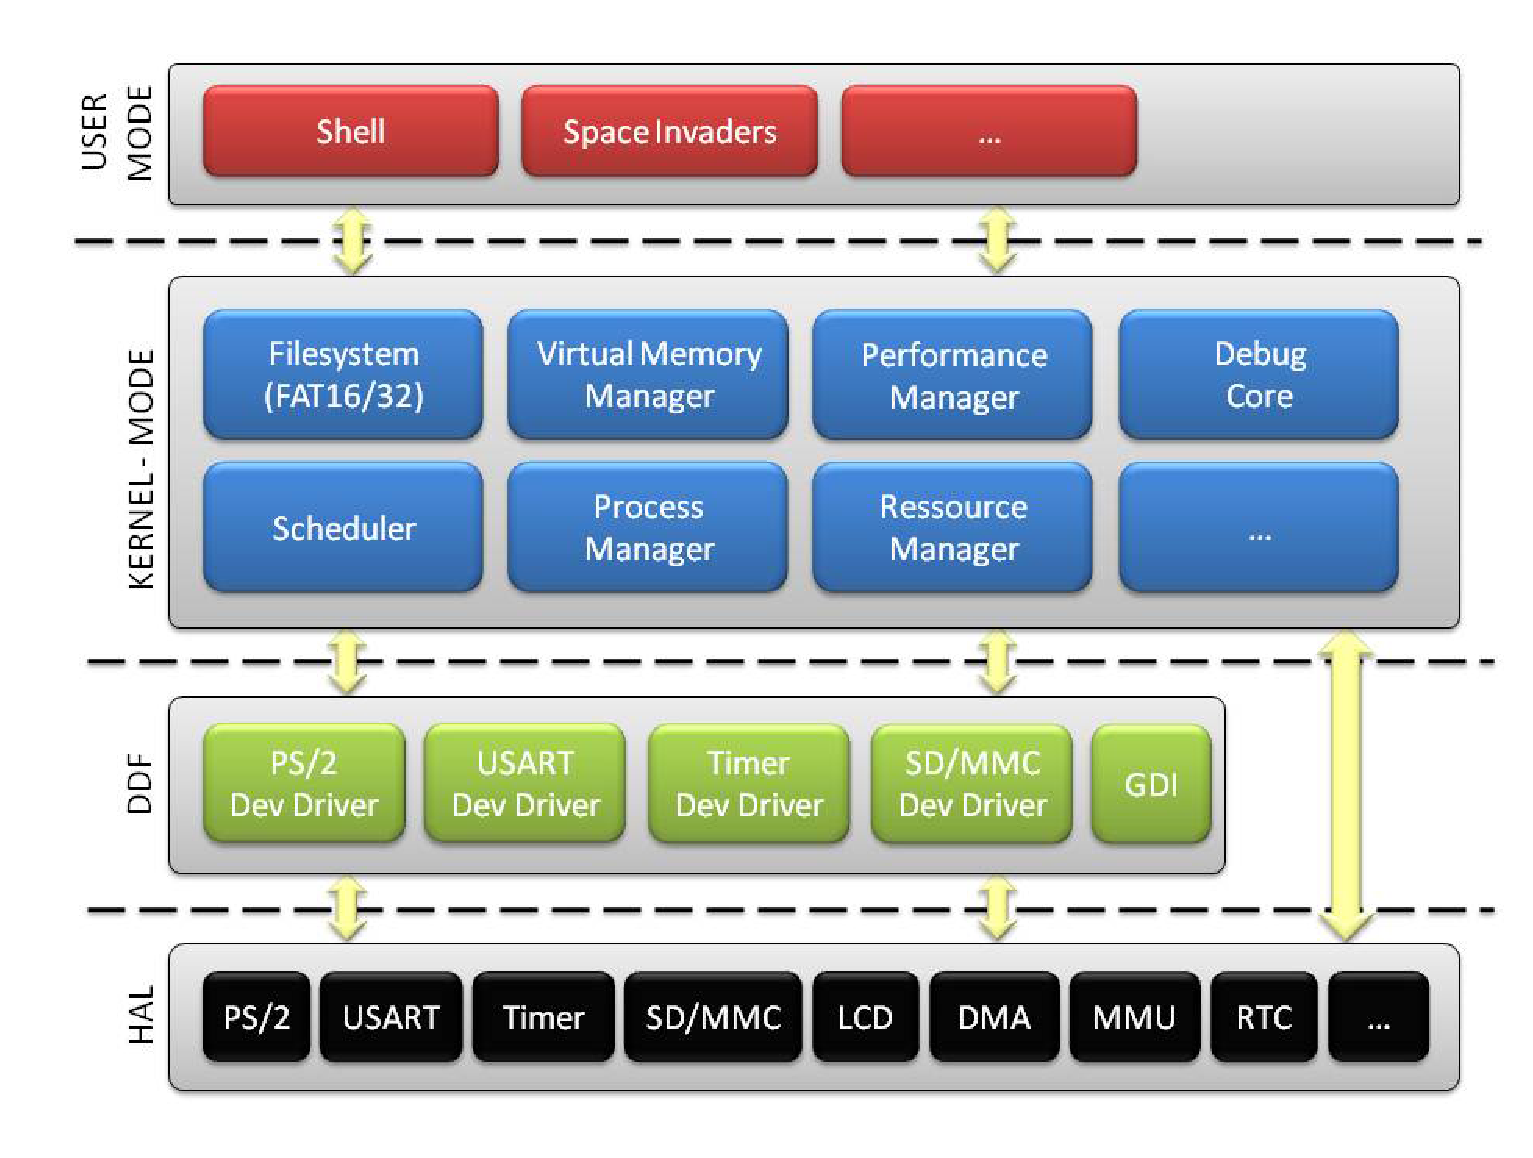
\includegraphics[width=10cm]{overview}\caption{Architecture Overview}
\end{center}
\end{Image}
\hypertarget{index_compinfo}{}\section{Compilation Info}\label{index_compinfo}
This software was written for the GNU GCC for AVR32\hypertarget{index_deviceinfo}{}\section{Device Info}\label{index_deviceinfo}
Currently there ist only support for AVR32 AP7000 devices\hypertarget{index_Example1}{}\section{Testscreen}\label{index_Example1}
CPU speed: {\em 150 MHz\/}\hypertarget{index_contactinfo}{}\section{Contact Info}\label{index_contactinfo}
For more info about HalOS \href{http://}{\tt Halos} \par
 Support mail: \href{mailto:test@test.com}{\tt test@test.com} 
\chapter{License}
\label{License}
\hypertarget{License}{}
GNU LESSER GENERAL PUBLIC LICENSE Version 2.1, February 1999

Copyright (C) 1991, 1999 Free Software Foundation, Inc. 51 Franklin Street, Fifth Floor, Boston, MA 02110-1301 USA Everyone is permitted to copy and distribute verbatim copies of this license document, but changing it is not allowed.

\mbox{[}This is the first released version of the Lesser GPL. It also counts as the successor of the GNU Library Public License, version 2, hence the version number 2.1.\mbox{]}

Preamble

The licenses for most software are designed to take away your freedom to share and change it. By contrast, the GNU General Public Licenses are intended to guarantee your freedom to share and change free software--to make sure the software is free for all its users.

This license, the Lesser General Public License, applies to some specially designated software packages--typically libraries--of the Free Software Foundation and other authors who decide to use it. You can use it too, but we suggest you first think carefully about whether this license or the ordinary General Public License is the better strategy to use in any particular case, based on the explanations below.

When we speak of free software, we are referring to freedom of use, not price. Our General Public Licenses are designed to make sure that you have the freedom to distribute copies of free software (and charge for this service if you wish); that you receive source code or can get it if you want it; that you can change the software and use pieces of it in new free programs; and that you are informed that you can do these things.

To protect your rights, we need to make restrictions that forbid distributors to deny you these rights or to ask you to surrender these rights. These restrictions translate to certain responsibilities for you if you distribute copies of the library or if you modify it.

For example, if you distribute copies of the library, whether gratis or for a fee, you must give the recipients all the rights that we gave you. You must make sure that they, too, receive or can get the source code. If you link other code with the library, you must provide complete object files to the recipients, so that they can relink them with the library after making changes to the library and recompiling it. And you must show them these terms so they know their rights.

We protect your rights with a two-step method: (1) we copyright the library, and (2) we offer you this license, which gives you legal permission to copy, distribute and/or modify the library.

To protect each distributor, we want to make it very clear that there is no warranty for the free library. Also, if the library is modified by someone else and passed on, the recipients should know that what they have is not the original version, so that the original author's reputation will not be affected by problems that might be introduced by others.

Finally, software patents pose a constant threat to the existence of any free program. We wish to make sure that a company cannot effectively restrict the users of a free program by obtaining a restrictive license from a patent holder. Therefore, we insist that any patent license obtained for a version of the library must be consistent with the full freedom of use specified in this license.

Most GNU software, including some libraries, is covered by the ordinary GNU General Public License. This license, the GNU Lesser General Public License, applies to certain designated libraries, and is quite different from the ordinary General Public License. We use this license for certain libraries in order to permit linking those libraries into non-free programs.

When a program is linked with a library, whether statically or using a shared library, the combination of the two is legally speaking a combined work, a derivative of the original library. The ordinary General Public License therefore permits such linking only if the entire combination fits its criteria of freedom. The Lesser General Public License permits more lax criteria for linking other code with the library.

We call this license the \char`\"{}Lesser\char`\"{} General Public License because it does Less to protect the user's freedom than the ordinary General Public License. It also provides other free software developers Less of an advantage over competing non-free programs. These disadvantages are the reason we use the ordinary General Public License for many libraries. However, the Lesser license provides advantages in certain special circumstances.

For example, on rare occasions, there may be a special need to encourage the widest possible use of a certain library, so that it becomes a de-facto standard. To achieve this, non-free programs must be allowed to use the library. A more frequent case is that a free library does the same job as widely used non-free libraries. In this case, there is little to gain by limiting the free library to free software only, so we use the Lesser General Public License.

In other cases, permission to use a particular library in non-free programs enables a greater number of people to use a large body of free software. For example, permission to use the GNU C Library in non-free programs enables many more people to use the whole GNU operating system, as well as its variant, the GNU/Linux operating system.

Although the Lesser General Public License is Less protective of the users' freedom, it does ensure that the user of a program that is linked with the Library has the freedom and the wherewithal to run that program using a modified version of the Library.

The precise terms and conditions for copying, distribution and modification follow. Pay close attention to the difference between a \char`\"{}work based on the library\char`\"{} and a \char`\"{}work that uses the library\char`\"{}. The former contains code derived from the library, whereas the latter must be combined with the library in order to run.

GNU LESSER GENERAL PUBLIC LICENSE TERMS AND CONDITIONS FOR COPYING, DISTRIBUTION AND MODIFICATION

0. This License Agreement applies to any software library or other program which contains a notice placed by the copyright holder or other authorized party saying it may be distributed under the terms of this Lesser General Public License (also called \char`\"{}this License\char`\"{}). Each licensee is addressed as \char`\"{}you\char`\"{}.

A \char`\"{}library\char`\"{} means a collection of software functions and/or data prepared so as to be conveniently linked with application programs (which use some of those functions and data) to form executables.

The \char`\"{}Library\char`\"{}, below, refers to any such software library or work which has been distributed under these terms. A \char`\"{}work based on the Library\char`\"{} means either the Library or any derivative work under copyright law: that is to say, a work containing the Library or a portion of it, either verbatim or with modifications and/or translated straightforwardly into another language. (Hereinafter, translation is included without limitation in the term \char`\"{}modification\char`\"{}.)

\char`\"{}Source code\char`\"{} for a work means the preferred form of the work for making modifications to it. For a library, complete source code means all the source code for all modules it contains, plus any associated interface definition files, plus the scripts used to control compilation and installation of the library.

Activities other than copying, distribution and modification are not covered by this License; they are outside its scope. The act of running a program using the Library is not restricted, and output from such a program is covered only if its contents constitute a work based on the Library (independent of the use of the Library in a tool for writing it). Whether that is true depends on what the Library does and what the program that uses the Library does.

1. You may copy and distribute verbatim copies of the Library's complete source code as you receive it, in any medium, provided that you conspicuously and appropriately publish on each copy an appropriate copyright notice and disclaimer of warranty; keep intact all the notices that refer to this License and to the absence of any warranty; and distribute a copy of this License along with the Library.

You may charge a fee for the physical act of transferring a copy, and you may at your option offer warranty protection in exchange for a fee.

2. You may modify your copy or copies of the Library or any portion of it, thus forming a work based on the Library, and copy and distribute such modifications or work under the terms of Section 1 above, provided that you also meet all of these conditions:

a) The modified work must itself be a software library.

b) You must cause the files modified to carry prominent notices stating that you changed the files and the date of any change.

c) You must cause the whole of the work to be licensed at no charge to all third parties under the terms of this License.

d) If a facility in the modified Library refers to a function or a table of data to be supplied by an application program that uses the facility, other than as an argument passed when the facility is invoked, then you must make a good faith effort to ensure that, in the event an application does not supply such function or table, the facility still operates, and performs whatever part of its purpose remains meaningful.

(For example, a function in a library to compute square roots has a purpose that is entirely well-defined independent of the application. Therefore, Subsection 2d requires that any application-supplied function or table used by this function must be optional: if the application does not supply it, the square root function must still compute square roots.)

These requirements apply to the modified work as a whole. If identifiable sections of that work are not derived from the Library, and can be reasonably considered independent and separate works in themselves, then this License, and its terms, do not apply to those sections when you distribute them as separate works. But when you distribute the same sections as part of a whole which is a work based on the Library, the distribution of the whole must be on the terms of this License, whose permissions for other licensees extend to the entire whole, and thus to each and every part regardless of who wrote it.

Thus, it is not the intent of this section to claim rights or contest your rights to work written entirely by you; rather, the intent is to exercise the right to control the distribution of derivative or collective works based on the Library.

In addition, mere aggregation of another work not based on the Library with the Library (or with a work based on the Library) on a volume of a storage or distribution medium does not bring the other work under the scope of this License.

3. You may opt to apply the terms of the ordinary GNU General Public License instead of this License to a given copy of the Library. To do this, you must alter all the notices that refer to this License, so that they refer to the ordinary GNU General Public License, version 2, instead of to this License. (If a newer version than version 2 of the ordinary GNU General Public License has appeared, then you can specify that version instead if you wish.) Do not make any other change in these notices.

Once this change is made in a given copy, it is irreversible for that copy, so the ordinary GNU General Public License applies to all subsequent copies and derivative works made from that copy.

This option is useful when you wish to copy part of the code of the Library into a program that is not a library.

4. You may copy and distribute the Library (or a portion or derivative of it, under Section 2) in object code or executable form under the terms of Sections 1 and 2 above provided that you accompany it with the complete corresponding machine-readable source code, which must be distributed under the terms of Sections 1 and 2 above on a medium customarily used for software interchange.

If distribution of object code is made by offering access to copy from a designated place, then offering equivalent access to copy the source code from the same place satisfies the requirement to distribute the source code, even though third parties are not compelled to copy the source along with the object code.

5. A program that contains no derivative of any portion of the Library, but is designed to work with the Library by being compiled or linked with it, is called a \char`\"{}work that uses the Library\char`\"{}. Such a work, in isolation, is not a derivative work of the Library, and therefore falls outside the scope of this License.

However, linking a \char`\"{}work that uses the Library\char`\"{} with the Library creates an executable that is a derivative of the Library (because it contains portions of the Library), rather than a \char`\"{}work that uses the library\char`\"{}. The executable is therefore covered by this License. Section 6 states terms for distribution of such executables.

When a \char`\"{}work that uses the Library\char`\"{} uses material from a header file that is part of the Library, the object code for the work may be a derivative work of the Library even though the source code is not. Whether this is true is especially significant if the work can be linked without the Library, or if the work is itself a library. The threshold for this to be true is not precisely defined by law.

If such an object file uses only numerical parameters, data structure layouts and accessors, and small macros and small inline functions (ten lines or less in length), then the use of the object file is unrestricted, regardless of whether it is legally a derivative work. (Executables containing this object code plus portions of the Library will still fall under Section 6.)

Otherwise, if the work is a derivative of the Library, you may distribute the object code for the work under the terms of Section 6. Any executables containing that work also fall under Section 6, whether or not they are linked directly with the Library itself.

6. As an exception to the Sections above, you may also combine or link a \char`\"{}work that uses the Library\char`\"{} with the Library to produce a work containing portions of the Library, and distribute that work under terms of your choice, provided that the terms permit modification of the work for the customer's own use and reverse engineering for debugging such modifications.

You must give prominent notice with each copy of the work that the Library is used in it and that the Library and its use are covered by this License. You must supply a copy of this License. If the work during execution displays copyright notices, you must include the copyright notice for the Library among them, as well as a reference directing the user to the copy of this License. Also, you must do one of these things:

a) Accompany the work with the complete corresponding machine-readable source code for the Library including whatever changes were used in the work (which must be distributed under Sections 1 and 2 above); and, if the work is an executable linked with the Library, with the complete machine-readable \char`\"{}work that uses the Library\char`\"{}, as object code and/or source code, so that the user can modify the Library and then relink to produce a modified executable containing the modified Library. (It is understood that the user who changes the contents of definitions files in the Library will not necessarily be able to recompile the application to use the modified definitions.)

b) Use a suitable shared library mechanism for linking with the Library. A suitable mechanism is one that (1) uses at run time a copy of the library already present on the user's computer system, rather than copying library functions into the executable, and (2) will operate properly with a modified version of the library, if the user installs one, as long as the modified version is interface-compatible with the version that the work was made with.

c) Accompany the work with a written offer, valid for at least three years, to give the same user the materials specified in Subsection 6a, above, for a charge no more than the cost of performing this distribution.

d) If distribution of the work is made by offering access to copy from a designated place, offer equivalent access to copy the above specified materials from the same place.

e) Verify that the user has already received a copy of these materials or that you have already sent this user a copy.

For an executable, the required form of the \char`\"{}work that uses the Library\char`\"{} must include any data and utility programs needed for reproducing the executable from it. However, as a special exception, the materials to be distributed need not include anything that is normally distributed (in either source or binary form) with the major components (compiler, kernel, and so on) of the operating system on which the executable runs, unless that component itself accompanies the executable.

It may happen that this requirement contradicts the license restrictions of other proprietary libraries that do not normally accompany the operating system. Such a contradiction means you cannot use both them and the Library together in an executable that you distribute.

7. You may place library facilities that are a work based on the Library side-by-side in a single library together with other library facilities not covered by this License, and distribute such a combined library, provided that the separate distribution of the work based on the Library and of the other library facilities is otherwise permitted, and provided that you do these two things:

a) Accompany the combined library with a copy of the same work based on the Library, uncombined with any other library facilities. This must be distributed under the terms of the Sections above.

b) Give prominent notice with the combined library of the fact that part of it is a work based on the Library, and explaining where to find the accompanying uncombined form of the same work.

8. You may not copy, modify, sublicense, link with, or distribute the Library except as expressly provided under this License. Any attempt otherwise to copy, modify, sublicense, link with, or distribute the Library is void, and will automatically terminate your rights under this License. However, parties who have received copies, or rights, from you under this License will not have their licenses terminated so long as such parties remain in full compliance.

9. You are not required to accept this License, since you have not signed it. However, nothing else grants you permission to modify or distribute the Library or its derivative works. These actions are prohibited by law if you do not accept this License. Therefore, by modifying or distributing the Library (or any work based on the Library), you indicate your acceptance of this License to do so, and all its terms and conditions for copying, distributing or modifying the Library or works based on it.

10. Each time you redistribute the Library (or any work based on the Library), the recipient automatically receives a license from the original licensor to copy, distribute, link with or modify the Library subject to these terms and conditions. You may not impose any further restrictions on the recipients' exercise of the rights granted herein. You are not responsible for enforcing compliance by third parties with this License.

11. If, as a consequence of a court judgment or allegation of patent infringement or for any other reason (not limited to patent issues), conditions are imposed on you (whether by court order, agreement or otherwise) that contradict the conditions of this License, they do not excuse you from the conditions of this License. If you cannot distribute so as to satisfy simultaneously your obligations under this License and any other pertinent obligations, then as a consequence you may not distribute the Library at all. For example, if a patent license would not permit royalty-free redistribution of the Library by all those who receive copies directly or indirectly through you, then the only way you could satisfy both it and this License would be to refrain entirely from distribution of the Library.

If any portion of this section is held invalid or unenforceable under any particular circumstance, the balance of the section is intended to apply, and the section as a whole is intended to apply in other circumstances.

It is not the purpose of this section to induce you to infringe any patents or other property right claims or to contest validity of any such claims; this section has the sole purpose of protecting the integrity of the free software distribution system which is implemented by public license practices. Many people have made generous contributions to the wide range of software distributed through that system in reliance on consistent application of that system; it is up to the author/donor to decide if he or she is willing to distribute software through any other system and a licensee cannot impose that choice.

This section is intended to make thoroughly clear what is believed to be a consequence of the rest of this License.

12. If the distribution and/or use of the Library is restricted in certain countries either by patents or by copyrighted interfaces, the original copyright holder who places the Library under this License may add an explicit geographical distribution limitation excluding those countries, so that distribution is permitted only in or among countries not thus excluded. In such case, this License incorporates the limitation as if written in the body of this License.

13. The Free Software Foundation may publish revised and/or new versions of the Lesser General Public License from time to time. Such new versions will be similar in spirit to the present version, but may differ in detail to address new problems or concerns.

Each version is given a distinguishing version number. If the Library specifies a version number of this License which applies to it and \char`\"{}any later version\char`\"{}, you have the option of following the terms and conditions either of that version or of any later version published by the Free Software Foundation. If the Library does not specify a license version number, you may choose any version ever published by the Free Software Foundation.

14. If you wish to incorporate parts of the Library into other free programs whose distribution conditions are incompatible with these, write to the author to ask for permission. For software which is copyrighted by the Free Software Foundation, write to the Free Software Foundation; we sometimes make exceptions for this. Our decision will be guided by the two goals of preserving the free status of all derivatives of our free software and of promoting the sharing and reuse of software generally.

NO WARRANTY

15. BECAUSE THE LIBRARY IS LICENSED FREE OF CHARGE, THERE IS NO WARRANTY FOR THE LIBRARY, TO THE EXTENT PERMITTED BY APPLICABLE LAW. EXCEPT WHEN OTHERWISE STATED IN WRITING THE COPYRIGHT HOLDERS AND/OR OTHER PARTIES PROVIDE THE LIBRARY \char`\"{}AS IS\char`\"{} WITHOUT WARRANTY OF ANY KIND, EITHER EXPRESSED OR IMPLIED, INCLUDING, BUT NOT LIMITED TO, THE IMPLIED WARRANTIES OF MERCHANTABILITY AND FITNESS FOR A PARTICULAR PURPOSE. THE ENTIRE RISK AS TO THE QUALITY AND PERFORMANCE OF THE LIBRARY IS WITH YOU. SHOULD THE LIBRARY PROVE DEFECTIVE, YOU ASSUME THE COST OF ALL NECESSARY SERVICING, REPAIR OR CORRECTION.

16. IN NO EVENT UNLESS REQUIRED BY APPLICABLE LAW OR AGREED TO IN WRITING WILL ANY COPYRIGHT HOLDER, OR ANY OTHER PARTY WHO MAY MODIFY AND/OR REDISTRIBUTE THE LIBRARY AS PERMITTED ABOVE, BE LIABLE TO YOU FOR DAMAGES, INCLUDING ANY GENERAL, SPECIAL, INCIDENTAL OR CONSEQUENTIAL DAMAGES ARISING OUT OF THE USE OR INABILITY TO USE THE LIBRARY (INCLUDING BUT NOT LIMITED TO LOSS OF DATA OR DATA BEING RENDERED INACCURATE OR LOSSES SUSTAINED BY YOU OR THIRD PARTIES OR A FAILURE OF THE LIBRARY TO OPERATE WITH ANY OTHER SOFTWARE), EVEN IF SUCH HOLDER OR OTHER PARTY HAS BEEN ADVISED OF THE POSSIBILITY OF SUCH DAMAGES.

END OF TERMS AND CONDITIONS 
\chapter{Installation}
\label{Installation}
\hypertarget{Installation}{}
\hypertarget{index_intro}{}\section{Introduction}\label{index_intro}
This Installation Guide shows how to install HalOS on the AVR NGW100 embedded board.\hypertarget{installation_Hardware}{}\section{and Tools}\label{installation_Hardware}
The following Tools for the HalOS installation are needed: \begin{itemize}
\item HW: ATMEL AVR NGW100 (with LCD Display, 480 x 272 ) \item HW: AVR JTAGICE mkII Debugger Device of ATMEL \item HW: Serial cable (for UART communication) \item SW: Integrated Development Environment (IDE) AMTEL AVR32 Studio, Version: 2.1.0 (JTAGICE mkII) \item SW: ATMEL AVR32 GNU Toolchain 2.1.4 Additional Tools (but not required): \item Subclipse for SVN \item CUnit for Testing \item Doxygen for documentation generation\end{itemize}
\hypertarget{installation_Bring}{}\section{HalOS and the Applications onto the NGW100}\label{installation_Bring}
In order to run HalOS on the NGW100 board the following steps have be done:\begin{enumerate}
\item Start AVR32 Studio and make sure that the JTAGICE mkII is recognized by AVR32 Studio\item Setup the JTAGICE mkII device in AVR32 Studio (first do \char`\"{}scan targets\char`\"{} and setup to the CPU: AP7000 and to the board: NGW100)\item Open and Execute (run) the HalOS Project on the AVR32 Studio (this will burn the HalOS on the board)\item Burn the HalOS applications to the Flash with the following parameters: \begin{itemize}
\item IdleProcess -$>$ File: IdleProcess.bin, Start Address: 0x00500000 \item Shell: -$>$ File: Shell.bin, Start Address: 0x00520000 \item SpaceInvaders: -$>$ File: SpaceInvaders.bin, Start Address: 0x00540000 \item ImageShow: -$>$ File: PhotoFrame.bin, Start Address: 0x00560000\end{itemize}
\item Now the HalOS System is ready to run and also ready to debug. Just restart the NGW100 by the reset button or power plug and be sure that the NGW100 is connected by the serial cable to a computer with a running terminal (E.g. HTerm).\end{enumerate}
\hypertarget{installation_Commands}{}\section{for the HalOS System: Shell, SpaceInvaders and ImageView}\label{installation_Commands}
The operating system starts by default the idle process as the first system application. Afterwards the idle process starts the shell applications, which is the basic process for user interactions. With the shell application the user is able to start new applications (like SpaceInvaders or ImageShow). After starting a new applications via the shell, the new applications is running an available to the user immediately (GUI and UART). The commands for the applications have to be entered via the UART (serial) terminal. The following commands are available:

SpaceInvaders: \begin{itemize}
\item \char`\"{}s\char`\"{} = shot \item \char`\"{}d\char`\"{} = right \item \char`\"{}a\char`\"{} = left \item \char`\"{}o\char`\"{} = Shutdown the application (quit)\end{itemize}
ImageShow:\begin{itemize}
\item has no commands, it runs automatic and switches through several images after around 5 seconds\end{itemize}


Shell:\begin{itemize}
\item start PROCESSNAME (E.g. \char`\"{}start SpaceInvaders\char`\"{}, \char`\"{}start ImageShow\char`\"{} )\item kill PROCESS-ID (E.g. \char`\"{}kill 3\char`\"{});\item top -$>$ shows the current processes in HalOS\item help -$>$ shows the available commands for the shell\item history -$>$ shows the last entered shell commands\item clear -$>$ clears the screen of the shell\end{itemize}


Its also possible to switch between different processes, therefore use: Ctrl + Alt + $|$ 
\chapter{Module Index}
\section{Modules}
Here is a list of all modules:\begin{CompactList}
\item \contentsline{section}{Halos Devices}{\pageref{group___d_e_v_i_c_e}}{}
\begin{CompactList}
\item \contentsline{section}{Device independend structure}{\pageref{group__device__driver}}{}
\item \contentsline{section}{Halos GDI}{\pageref{group___g_d_i___d_e_v_i_c_e}}{}
\begin{CompactList}
\item \contentsline{section}{Halos Font}{\pageref{group___f_o_n_t_s}}{}
\begin{CompactList}
\item \contentsline{section}{Arial Bold 14 Font}{\pageref{group__graphic__device__font__arial14}}{}
\item \contentsline{section}{Handel Bold 14 Font}{\pageref{group__graphic__device__font__handel14}}{}
\item \contentsline{section}{Font}{\pageref{group__graphic__device__font}}{}
\end{CompactList}
\item \contentsline{section}{Graphic Device}{\pageref{group__graphic__device}}{}
\item \contentsline{section}{Graphic Hardware Interface}{\pageref{group__graphic__hw__interface}}{}
\end{CompactList}
\item \contentsline{section}{Hardware dependent}{\pageref{group___d_e_v_i_c_e___p_o_r_t_s}}{}
\begin{CompactList}
\item \contentsline{section}{AP7000}{\pageref{group___a_p7}}{}
\begin{CompactList}
\item \contentsline{section}{Hardware Devices}{\pageref{group__ap7000__hardware__devices}}{}
\begin{CompactList}
\item \contentsline{section}{DEV\_\-NULL Driver}{\pageref{group___d_e_v___n_u_l_l___d_r_i_v_e_r}}{}
\item \contentsline{section}{Led Driver}{\pageref{group___l_e_d___d_r_i_v_e_r}}{}
\item \contentsline{section}{UART Driver}{\pageref{group___u_a_r_t___d_r_i_v_e_r}}{}
\end{CompactList}
\item \contentsline{section}{LCD}{\pageref{group__ap7000__lcd}}{}
\end{CompactList}
\end{CompactList}
\end{CompactList}
\item \contentsline{section}{Hardware Abstraction Layer}{\pageref{group__haloshal}}{}
\begin{CompactList}
\item \contentsline{section}{halos interrupt driven UART}{\pageref{group___u_a_r_t}}{}
\item \contentsline{section}{Serial Buffer for Halos UART}{\pageref{group__serialbuffer}}{}
\end{CompactList}
\item \contentsline{section}{Halos API's}{\pageref{group___a_p_i}}{}
\begin{CompactList}
\item \contentsline{section}{Halos Device Api}{\pageref{group___d_e_v_i_c_e___a_p_i}}{}
\begin{CompactList}
\item \contentsline{section}{AP7000 specific devices}{\pageref{group___a_p7000___d_e_v}}{}
\end{CompactList}
\item \contentsline{section}{Halos GDI}{\pageref{group___g_d_i}}{}
\begin{CompactList}
\item \contentsline{section}{16-bit Colors}{\pageref{group__hgdi__colors16}}{}
\item \contentsline{section}{24-bit Colors}{\pageref{group__hgdi__colors24}}{}
\item \contentsline{section}{8-bit Colors}{\pageref{group__hgdi__colors8}}{}
\item \contentsline{section}{Fonts}{\pageref{group__hgdi__fonts}}{}
\item \contentsline{section}{GDI Types}{\pageref{group__hgdi__types}}{}
\item \contentsline{section}{GDI API}{\pageref{group__hgdi__api}}{}
\end{CompactList}
\item \contentsline{section}{System Call API}{\pageref{group___s_y_s_t_e_m___c_a_l_l___a_p_i}}{}
\begin{CompactList}
\item \contentsline{section}{System API}{\pageref{group___h_s_y_s_t_e_m___a_p_i}}{}
\item \contentsline{section}{System Call Table}{\pageref{group___s_y_s_t_e_m___c_a_l_l___t_a_b_l_e}}{}
\end{CompactList}
\item \contentsline{section}{Utilitys}{\pageref{group___u_t_i_l}}{}
\begin{CompactList}
\item \contentsline{section}{System Time API}{\pageref{group___t_i_m_e_a_p_i}}{}
\item \contentsline{section}{Utils for HalOS}{\pageref{group___u_t_i_l_i_t_y_s}}{}
\end{CompactList}
\end{CompactList}
\item \contentsline{section}{Halos Kernel}{\pageref{group___k_e_r_n_e_l}}{}
\begin{CompactList}
\item \contentsline{section}{Halos Configurations}{\pageref{group___c_o_n_f_i_g}}{}
\item \contentsline{section}{Halos Globals}{\pageref{group___g_l_o_b_a_l_s}}{}
\item \contentsline{section}{Error Types}{\pageref{group___e_r_r_o_r_t_y_p_e_s}}{}
\item \contentsline{section}{Time - Halos System Ticks}{\pageref{group___t_i_m_e}}{}
\item \contentsline{section}{Board Initialization}{\pageref{group___i_n_i_t}}{}
\item \contentsline{section}{Process Manager}{\pageref{group___p_r_o_c_e_s_s___m_a_n_a_g_e_r}}{}
\begin{CompactList}
\item \contentsline{section}{Process Control Block (PCB)}{\pageref{group___p_c_b}}{}
\item \contentsline{section}{Scheduler}{\pageref{group___s_c_h_e_d_u_l_e_r}}{}
\item \contentsline{section}{Halos Portings for AVR AP7000}{\pageref{group___p_o_r_t_i_n_g_s_a_p7000}}{}
\end{CompactList}
\item \contentsline{section}{Resource Manager}{\pageref{group___r_e_s_o_u_r_c_e___m_a_n_a_g_e_r}}{}
\begin{CompactList}
\item \contentsline{section}{Hashmap for Resource Manager}{\pageref{group___h_a_s_h_m_a_p}}{}
\item \contentsline{section}{Resource Manager for device access}{\pageref{group___r_e_s_o_u_r_c_e___m}}{}
\end{CompactList}
\item \contentsline{section}{System Call Handler}{\pageref{group___s_y_s_t_e_m___c_a_l_l___h_a_n_d_l_e_r}}{}
\item \contentsline{section}{Virtual Memory Management}{\pageref{group___v_m_m}}{}
\begin{CompactList}
\item \contentsline{section}{Hash Anchor Table}{\pageref{group___v_m_m___h_a_t}}{}
\item \contentsline{section}{Heap Management}{\pageref{group___v_m_m___h_e_a_p}}{}
\item \contentsline{section}{iHex Parser}{\pageref{group___v_m_m___h_e_x}}{}
\item \contentsline{section}{Inverted Page Table}{\pageref{group___v_m_m___i_p_t}}{}
\item \contentsline{section}{Loader}{\pageref{group___v_m_m___l_d_r}}{}
\item \contentsline{section}{Page Table}{\pageref{group___v_m_m___p_t}}{}
\item \contentsline{section}{Page Table Entry}{\pageref{group___v_m_m___p_t_e}}{}
\item \contentsline{section}{Process Region Table}{\pageref{group___v_m_m___p_r_t}}{}
\item \contentsline{section}{Transition Lookaside Buffer}{\pageref{group___v_m_m___t_l_b}}{}
\end{CompactList}
\end{CompactList}
\end{CompactList}

\chapter{Data Structure Index}
\section{Data Structures}
Here are the data structures with brief descriptions:\begin{CompactList}
\item\contentsline{section}{\hyperlink{struct__gdi__sprite}{\_\-gdi\_\-sprite} (Struct that defines a gdi sprite )}{\pageref{struct__gdi__sprite}}{}
\item\contentsline{section}{\hyperlink{structaccess__entry}{access\_\-entry} (Planned to implement access entries to handle accesses from processes to devices )}{\pageref{structaccess__entry}}{}
\item\contentsline{section}{\hyperlink{struct_binary}{Binary} }{\pageref{struct_binary}}{}
\item\contentsline{section}{\hyperlink{struct_cursor__t}{Cursor\_\-t} (Struct that defines the position of the cursor )}{\pageref{struct_cursor__t}}{}
\item\contentsline{section}{\hyperlink{struct_device_context__t}{DeviceContext\_\-t} (Struct that defines the device context )}{\pageref{struct_device_context__t}}{}
\item\contentsline{section}{\hyperlink{struct_display_info__t}{DisplayInfo\_\-t} (Struct that defines Display information )}{\pageref{struct_display_info__t}}{}
\item\contentsline{section}{\hyperlink{struct_font_settings__t}{FontSettings\_\-t} (Struct that defines the font settings )}{\pageref{struct_font_settings__t}}{}
\item\contentsline{section}{\hyperlink{structlcdc__configuration__s}{lcdc\_\-configuration\_\-s} (Struct that defines the configuration of the LCD controller )}{\pageref{structlcdc__configuration__s}}{}
\item\contentsline{section}{\hyperlink{struct_line_settings__t}{LineSettings\_\-t} (Struct that defines the linestyle )}{\pageref{struct_line_settings__t}}{}
\item\contentsline{section}{\hyperlink{structmmu__tlb__t}{mmu\_\-tlb\_\-t} (Struct which defines options for operating on TLB entries )}{\pageref{structmmu__tlb__t}}{}
\item\contentsline{section}{\hyperlink{struct_pager}{Pager} }{\pageref{struct_pager}}{}
\item\contentsline{section}{\hyperlink{struct_page_table}{PageTable} }{\pageref{struct_page_table}}{}
\item\contentsline{section}{\hyperlink{struct_page_table_entry}{PageTableEntry} }{\pageref{struct_page_table_entry}}{}
\item\contentsline{section}{\hyperlink{structpm__gen__clk__opt__t}{pm\_\-gen\_\-clk\_\-opt\_\-t} (Generic clock genration options )}{\pageref{structpm__gen__clk__opt__t}}{}
\item\contentsline{section}{\hyperlink{structpm__osc__opt__t}{pm\_\-osc\_\-opt\_\-t} (Oscilator startup options )}{\pageref{structpm__osc__opt__t}}{}
\item\contentsline{section}{\hyperlink{structpm__pll__opt__t}{pm\_\-pll\_\-opt\_\-t} (Pll settings. The new frequency will be set according to the following formula: pll = osc $\ast$ mul / div )}{\pageref{structpm__pll__opt__t}}{}
\item\contentsline{section}{\hyperlink{struct_process}{Process} }{\pageref{struct_process}}{}
\item\contentsline{section}{\hyperlink{structprocess_control_block}{processControlBlock} (Control Block for holding all the task informations, used mainly by the schuduler )}{\pageref{structprocess_control_block}}{}
\item\contentsline{section}{\hyperlink{struct_process_region}{ProcessRegion} }{\pageref{struct_process_region}}{}
\item\contentsline{section}{\hyperlink{struct_serial_buffer_tag}{SerialBufferTag} }{\pageref{struct_serial_buffer_tag}}{}
\item\contentsline{section}{\hyperlink{struct_time_tag}{TimeTag} }{\pageref{struct_time_tag}}{}
\item\contentsline{section}{\hyperlink{struct_t_l_b_e_h_i}{TLBEHI} }{\pageref{struct_t_l_b_e_h_i}}{}
\item\contentsline{section}{\hyperlink{struct_t_l_b_e_h_i_v_n_p_l_e_s_s}{TLBEHIVNPLESS} }{\pageref{struct_t_l_b_e_h_i_v_n_p_l_e_s_s}}{}
\item\contentsline{section}{\hyperlink{struct_t_l_b_e_l_o}{TLBELO} }{\pageref{struct_t_l_b_e_l_o}}{}
\item\contentsline{section}{\hyperlink{struct_t_l_b_e_l_o_p_f_n_l_e_s_s}{TLBELOPFNLESS} }{\pageref{struct_t_l_b_e_l_o_p_f_n_l_e_s_s}}{}
\item\contentsline{section}{\hyperlink{structusart__options__t}{usart\_\-options\_\-t} }{\pageref{structusart__options__t}}{}
\item\contentsline{section}{\hyperlink{structvirtual__dev__struct}{virtual\_\-dev\_\-struct} (Virtual device structure, which keeps track of the requested physical device. RXBuffer and TXbuffer are kept seperately for each virtual device )}{\pageref{structvirtual__dev__struct}}{}
\item\contentsline{section}{\hyperlink{structwaiting__node}{waiting\_\-node} (Planned to implement a waiting queue for ressources )}{\pageref{structwaiting__node}}{}
\end{CompactList}

\chapter{File Index}
\section{File List}
Here is a list of all documented files with brief descriptions:\begin{CompactList}
\item\contentsline{section}{E:/Ausbildung/Semester3/Kopie von AVR32\_\-Work1/Halos\_\-Development/src/\hyperlink{documentation_8h}{documentation.h} (Halos Operation System for AVR32 )}{\pageref{documentation_8h}}{}
\item\contentsline{section}{E:/Ausbildung/Semester3/Kopie von AVR32\_\-Work1/Halos\_\-Development/src/apps/\textbf{process1.h} }{\pageref{process1_8h}}{}
\item\contentsline{section}{E:/Ausbildung/Semester3/Kopie von AVR32\_\-Work1/Halos\_\-Development/src/apps/\textbf{process2.h} }{\pageref{process2_8h}}{}
\item\contentsline{section}{E:/Ausbildung/Semester3/Kopie von AVR32\_\-Work1/Halos\_\-Development/src/apps/\textbf{shell.h} }{\pageref{shell_8h}}{}
\item\contentsline{section}{E:/Ausbildung/Semester3/Kopie von AVR32\_\-Work1/Halos\_\-Development/src/devices/\hyperlink{device__driver_8h}{device\_\-driver.h} (Device Hardware Interface )}{\pageref{device__driver_8h}}{}
\item\contentsline{section}{E:/Ausbildung/Semester3/Kopie von AVR32\_\-Work1/Halos\_\-Development/src/devices/gdi/font/fonts/\textbf{arial\_\-10.h} }{\pageref{arial__10_8h}}{}
\item\contentsline{section}{E:/Ausbildung/Semester3/Kopie von AVR32\_\-Work1/Halos\_\-Development/src/devices/gdi/font/fonts/\hyperlink{arial__bold__14_8h}{arial\_\-bold\_\-14.h} (Arial bold 14 Font for Halos )}{\pageref{arial__bold__14_8h}}{}
\item\contentsline{section}{E:/Ausbildung/Semester3/Kopie von AVR32\_\-Work1/Halos\_\-Development/src/devices/gdi/font/fonts/\textbf{controlls.h} }{\pageref{controlls_8h}}{}
\item\contentsline{section}{E:/Ausbildung/Semester3/Kopie von AVR32\_\-Work1/Halos\_\-Development/src/devices/gdi/font/fonts/\textbf{corsiva\_\-12.h} }{\pageref{corsiva__12_8h}}{}
\item\contentsline{section}{E:/Ausbildung/Semester3/Kopie von AVR32\_\-Work1/Halos\_\-Development/src/devices/gdi/font/fonts/\textbf{FIVE\_\-DOT.h} }{\pageref{_f_i_v_e___d_o_t_8h}}{}
\item\contentsline{section}{E:/Ausbildung/Semester3/Kopie von AVR32\_\-Work1/Halos\_\-Development/src/devices/gdi/font/fonts/\hyperlink{handel__bold__14_8h}{handel\_\-bold\_\-14.h} (Handel Bold 14 Font for Halos )}{\pageref{handel__bold__14_8h}}{}
\item\contentsline{section}{E:/Ausbildung/Semester3/Kopie von AVR32\_\-Work1/Halos\_\-Development/src/devices/gdi/font/inc/\hyperlink{font_8h}{font.h} (Device independet graphic/font header )}{\pageref{font_8h}}{}
\item\contentsline{section}{E:/Ausbildung/Semester3/Kopie von AVR32\_\-Work1/Halos\_\-Development/src/devices/gdi/font/src/\hyperlink{font_8c}{font.c} (Device independet graphic/font implementation )}{\pageref{font_8c}}{}
\item\contentsline{section}{E:/Ausbildung/Semester3/Kopie von AVR32\_\-Work1/Halos\_\-Development/src/devices/gdi/graphics/inc/\hyperlink{graphics_8h}{graphics.h} (Device independent graphic code )}{\pageref{graphics_8h}}{}
\item\contentsline{section}{E:/Ausbildung/Semester3/Kopie von AVR32\_\-Work1/Halos\_\-Development/src/devices/gdi/graphics/inc/\hyperlink{graphis__hw__interface_8h}{graphis\_\-hw\_\-interface.h} (Graphics Hardware Interface )}{\pageref{graphis__hw__interface_8h}}{}
\item\contentsline{section}{E:/Ausbildung/Semester3/Kopie von AVR32\_\-Work1/Halos\_\-Development/src/devices/gdi/graphics/src/\hyperlink{graphics_8c}{graphics.c} (Device independent graphic code )}{\pageref{graphics_8c}}{}
\item\contentsline{section}{E:/Ausbildung/Semester3/Kopie von AVR32\_\-Work1/Halos\_\-Development/src/devices/ports/avr32/ap7x/ap7000/devices/\hyperlink{device__list_8h}{device\_\-list.h} (List of the devices on the board )}{\pageref{device__list_8h}}{}
\item\contentsline{section}{E:/Ausbildung/Semester3/Kopie von AVR32\_\-Work1/Halos\_\-Development/src/devices/ports/avr32/ap7x/ap7000/devices/dev\_\-null\_\-driver/inc/\hyperlink{dev__null__driver_8h}{dev\_\-null\_\-driver.h} (Dummy device for background processes )}{\pageref{dev__null__driver_8h}}{}
\item\contentsline{section}{E:/Ausbildung/Semester3/Kopie von AVR32\_\-Work1/Halos\_\-Development/src/devices/ports/avr32/ap7x/ap7000/devices/leds\_\-driver/\hyperlink{leds__driver_8h}{leds\_\-driver.h} (Hardware dependent led driver code )}{\pageref{leds__driver_8h}}{}
\item\contentsline{section}{E:/Ausbildung/Semester3/Kopie von AVR32\_\-Work1/Halos\_\-Development/src/devices/ports/avr32/ap7x/ap7000/devices/uart\_\-driver/\textbf{printf\_\-P.h} }{\pageref{printf___p_8h}}{}
\item\contentsline{section}{E:/Ausbildung/Semester3/Kopie von AVR32\_\-Work1/Halos\_\-Development/src/devices/ports/avr32/ap7x/ap7000/devices/uart\_\-driver/\hyperlink{uart__driver_8h}{uart\_\-driver.h} (Hardware dependent UART code )}{\pageref{uart__driver_8h}}{}
\item\contentsline{section}{E:/Ausbildung/Semester3/Kopie von AVR32\_\-Work1/Halos\_\-Development/src/devices/ports/avr32/ap7x/ap7000/displays/inc/\hyperlink{ap7000__lcd_8h}{ap7000\_\-lcd.h} (AP7000 hardware dependet graphic/lcd header )}{\pageref{ap7000__lcd_8h}}{}
\item\contentsline{section}{E:/Ausbildung/Semester3/Kopie von AVR32\_\-Work1/Halos\_\-Development/src/devices/ports/avr32/ap7x/ap7000/displays/inc/\textbf{ap7000\_\-lcd\_\-bg.h} }{\pageref{ap7000__lcd__bg_8h}}{}
\item\contentsline{section}{E:/Ausbildung/Semester3/Kopie von AVR32\_\-Work1/Halos\_\-Development/src/devices/ports/avr32/ap7x/ap7000/displays/src/\hyperlink{ap7000__lcd_8c}{ap7000\_\-lcd.c} (AP7000 hardware dependet graphic/lcd implementation )}{\pageref{ap7000__lcd_8c}}{}
\item\contentsline{section}{E:/Ausbildung/Semester3/Kopie von AVR32\_\-Work1/Halos\_\-Development/src/hal/ports/avr32/ap7x/ap7000/\hyperlink{compiler_8h}{compiler.h} (Compiler file for AVR32 )}{\pageref{compiler_8h}}{}
\item\contentsline{section}{E:/Ausbildung/Semester3/Kopie von AVR32\_\-Work1/Halos\_\-Development/src/hal/ports/avr32/ap7x/ap7000/\textbf{error.h} }{\pageref{error_8h}}{}
\item\contentsline{section}{E:/Ausbildung/Semester3/Kopie von AVR32\_\-Work1/Halos\_\-Development/src/hal/ports/avr32/ap7x/ap7000/\hyperlink{macro_8h}{macro.h} (MMU example application )}{\pageref{macro_8h}}{}
\item\contentsline{section}{E:/Ausbildung/Semester3/Kopie von AVR32\_\-Work1/Halos\_\-Development/src/hal/ports/avr32/ap7x/ap7000/\hyperlink{mmu_8c}{mmu.c} (MMU example application )}{\pageref{mmu_8c}}{}
\item\contentsline{section}{E:/Ausbildung/Semester3/Kopie von AVR32\_\-Work1/Halos\_\-Development/src/hal/ports/avr32/ap7x/ap7000/\hyperlink{mmu_8h}{mmu.h} (MMU example application )}{\pageref{mmu_8h}}{}
\item\contentsline{section}{E:/Ausbildung/Semester3/Kopie von AVR32\_\-Work1/Halos\_\-Development/src/hal/ports/avr32/ap7x/ap7000/\hyperlink{mt481c2m32b2tg_8h}{mt481c2m32b2tg.h} (MT481C2M32B2TG SDRAM driver for AVR32 SDRAMC on EBI )}{\pageref{mt481c2m32b2tg_8h}}{}
\item\contentsline{section}{E:/Ausbildung/Semester3/Kopie von AVR32\_\-Work1/Halos\_\-Development/src/hal/ports/avr32/ap7x/ap7000/\hyperlink{my__usart_8h}{my\_\-usart.h} (Interrupt driven UART )}{\pageref{my__usart_8h}}{}
\item\contentsline{section}{E:/Ausbildung/Semester3/Kopie von AVR32\_\-Work1/Halos\_\-Development/src/hal/ports/avr32/ap7x/ap7000/\textbf{ngw100.h} }{\pageref{ngw100_8h}}{}
\item\contentsline{section}{E:/Ausbildung/Semester3/Kopie von AVR32\_\-Work1/Halos\_\-Development/src/hal/ports/avr32/ap7x/ap7000/\hyperlink{pio_8c}{pio.c} (Pio driver functions )}{\pageref{pio_8c}}{}
\item\contentsline{section}{E:/Ausbildung/Semester3/Kopie von AVR32\_\-Work1/Halos\_\-Development/src/hal/ports/avr32/ap7x/ap7000/\hyperlink{pio_8h}{pio.h} (Pio driver functions )}{\pageref{pio_8h}}{}
\item\contentsline{section}{E:/Ausbildung/Semester3/Kopie von AVR32\_\-Work1/Halos\_\-Development/src/hal/ports/avr32/ap7x/ap7000/\hyperlink{pm__at32ap7000_8c}{pm\_\-at32ap7000.c} (Power Manager driver )}{\pageref{pm__at32ap7000_8c}}{}
\item\contentsline{section}{E:/Ausbildung/Semester3/Kopie von AVR32\_\-Work1/Halos\_\-Development/src/hal/ports/avr32/ap7x/ap7000/\hyperlink{pm__at32ap7000_8h}{pm\_\-at32ap7000.h} (Power Manager driver )}{\pageref{pm__at32ap7000_8h}}{}
\item\contentsline{section}{E:/Ausbildung/Semester3/Kopie von AVR32\_\-Work1/Halos\_\-Development/src/hal/ports/avr32/ap7x/ap7000/\hyperlink{sdramc_8h}{sdramc.h} (SDRAMC on EBI driver for AVR32 UC3 )}{\pageref{sdramc_8h}}{}
\item\contentsline{section}{E:/Ausbildung/Semester3/Kopie von AVR32\_\-Work1/Halos\_\-Development/src/hal/ports/avr32/ap7x/ap7000/\hyperlink{sdramc__at32ap7000_8c}{sdramc\_\-at32ap7000.c} (SDRAMC on EBI driver for AVR32 )}{\pageref{sdramc__at32ap7000_8c}}{}
\item\contentsline{section}{E:/Ausbildung/Semester3/Kopie von AVR32\_\-Work1/Halos\_\-Development/src/hal/ports/avr32/ap7x/ap7000/\hyperlink{sdramc__at32ap7000_8h}{sdramc\_\-at32ap7000.h} (SDRAMC on EBI driver for AVR32 )}{\pageref{sdramc__at32ap7000_8h}}{}
\item\contentsline{section}{E:/Ausbildung/Semester3/Kopie von AVR32\_\-Work1/Halos\_\-Development/src/hal/ports/avr32/ap7x/ap7000/\textbf{SerialBuffer.h} }{\pageref{_serial_buffer_8h}}{}
\item\contentsline{section}{E:/Ausbildung/Semester3/Kopie von AVR32\_\-Work1/Halos\_\-Development/src/hal/ports/avr32/ap7x/ap7000/\hyperlink{usart_8c}{usart.c} (USART driver library )}{\pageref{usart_8c}}{}
\item\contentsline{section}{E:/Ausbildung/Semester3/Kopie von AVR32\_\-Work1/Halos\_\-Development/src/hal/ports/avr32/ap7x/ap7000/\hyperlink{usart_8h}{usart.h} (USART driver library )}{\pageref{usart_8h}}{}
\item\contentsline{section}{E:/Ausbildung/Semester3/Kopie von AVR32\_\-Work1/Halos\_\-Development/src/hal/ports/avr32/ap7x/ap7000/\hyperlink{usart__isr_8h}{usart\_\-isr.h} (Interrupt driven UART handler code )}{\pageref{usart__isr_8h}}{}
\item\contentsline{section}{E:/Ausbildung/Semester3/Kopie von AVR32\_\-Work1/Halos\_\-Development/src/hal/ports/avr32/ap7x/ap7000/exceptions/inc/\hyperlink{exceptions_8h}{exceptions.h} (NEWLIB\_\-ADDONS exceptions include file for AVR32 )}{\pageref{exceptions_8h}}{}
\item\contentsline{section}{E:/Ausbildung/Semester3/Kopie von AVR32\_\-Work1/Halos\_\-Development/src/hal/ports/avr32/ap7x/ap7000/exceptions/inc/\textbf{mmu\_\-exceptions.h} }{\pageref{mmu__exceptions_8h}}{}
\item\contentsline{section}{E:/Ausbildung/Semester3/Kopie von AVR32\_\-Work1/Halos\_\-Development/src/hal/ports/avr32/ap7x/ap7000/exceptions/src/\hyperlink{exception__handling_8c}{exception\_\-handling.c} (NEWLIB\_\-ADDONS exception handling file for AVR32 )}{\pageref{exception__handling_8c}}{}
\item\contentsline{section}{E:/Ausbildung/Semester3/Kopie von AVR32\_\-Work1/Halos\_\-Development/src/hal/ports/avr32/ap7x/ap7000/interrupts/inc/\hyperlink{interrupts_8h}{interrupts.h} (NEWLIB\_\-ADDONS interrupts include file for AVR32 )}{\pageref{interrupts_8h}}{}
\item\contentsline{section}{E:/Ausbildung/Semester3/Kopie von AVR32\_\-Work1/Halos\_\-Development/src/hal/ports/avr32/ap7x/ap7000/interrupts/src/\hyperlink{interrupts_8c}{interrupts.c} (NEWLIB\_\-ADDONS interrupt handling file for AVR32 )}{\pageref{interrupts_8c}}{}
\item\contentsline{section}{E:/Ausbildung/Semester3/Kopie von AVR32\_\-Work1/Halos\_\-Development/src/hal/ports/avr32/ap7x/ap7000/newlib/\hyperlink{cpu_8c}{cpu.c} (NEWLIB\_\-ADDONS CPU management file for AVR32 )}{\pageref{cpu_8c}}{}
\item\contentsline{section}{E:/Ausbildung/Semester3/Kopie von AVR32\_\-Work1/Halos\_\-Development/src/hal/ports/avr32/ap7x/ap7000/newlib/\hyperlink{nlao__cpu_8h}{nlao\_\-cpu.h} (NEWLIB\_\-ADDONS CPU include file for AVR32 )}{\pageref{nlao__cpu_8h}}{}
\item\contentsline{section}{E:/Ausbildung/Semester3/Kopie von AVR32\_\-Work1/Halos\_\-Development/src/hal/ports/avr32/ap7x/ap7000/newlib/\hyperlink{nlao__io_8h}{nlao\_\-io.h} (NEWLIB\_\-ADDONS miscellaneous macros include file for AVR32 )}{\pageref{nlao__io_8h}}{}
\item\contentsline{section}{E:/Ausbildung/Semester3/Kopie von AVR32\_\-Work1/Halos\_\-Development/src/hal/ports/avr32/ap7x/ap7000/newlib/\hyperlink{syscalls_8c}{syscalls.c} (NEWLIB\_\-ADDONS system calls overloading file for AVR32 )}{\pageref{syscalls_8c}}{}
\item\contentsline{section}{E:/Ausbildung/Semester3/Kopie von AVR32\_\-Work1/Halos\_\-Development/src/hal/ports/avr32/ap7x/ap7000/newlib/\hyperlink{tpaste_8h}{tpaste.h} (Preprocessor token pasting utils )}{\pageref{tpaste_8h}}{}
\item\contentsline{section}{E:/Ausbildung/Semester3/Kopie von AVR32\_\-Work1/Halos\_\-Development/src/halos\_\-apis/halos\_\-device\_\-api/inc/\hyperlink{device__struct_8h}{device\_\-struct.h} (Device Structure )}{\pageref{device__struct_8h}}{}
\item\contentsline{section}{E:/Ausbildung/Semester3/Kopie von AVR32\_\-Work1/Halos\_\-Development/src/halos\_\-apis/halos\_\-device\_\-api/inc/\hyperlink{hdevice__api_8h}{hdevice\_\-api.h} (Device API header )}{\pageref{hdevice__api_8h}}{}
\item\contentsline{section}{E:/Ausbildung/Semester3/Kopie von AVR32\_\-Work1/Halos\_\-Development/src/halos\_\-apis/halos\_\-device\_\-api/ports/avr32/ap7x/ap7000/\hyperlink{device__types_8h}{device\_\-types.h} (AP7000 specific Device types )}{\pageref{device__types_8h}}{}
\item\contentsline{section}{E:/Ausbildung/Semester3/Kopie von AVR32\_\-Work1/Halos\_\-Development/src/halos\_\-apis/halos\_\-device\_\-api/src/\hyperlink{hdevice__api_8c}{hdevice\_\-api.c} (Device API implementation )}{\pageref{hdevice__api_8c}}{}
\item\contentsline{section}{E:/Ausbildung/Semester3/Kopie von AVR32\_\-Work1/Halos\_\-Development/src/halos\_\-apis/halos\_\-gdi/inc/\hyperlink{colors_8h}{colors.h} (Colortable )}{\pageref{colors_8h}}{}
\item\contentsline{section}{E:/Ausbildung/Semester3/Kopie von AVR32\_\-Work1/Halos\_\-Development/src/halos\_\-apis/halos\_\-gdi/inc/\hyperlink{colors16_8h}{colors16.h} (16-Bit Colortable )}{\pageref{colors16_8h}}{}
\item\contentsline{section}{E:/Ausbildung/Semester3/Kopie von AVR32\_\-Work1/Halos\_\-Development/src/halos\_\-apis/halos\_\-gdi/inc/\hyperlink{colors24_8h}{colors24.h} (24-Bit Colortable )}{\pageref{colors24_8h}}{}
\item\contentsline{section}{E:/Ausbildung/Semester3/Kopie von AVR32\_\-Work1/Halos\_\-Development/src/halos\_\-apis/halos\_\-gdi/inc/\hyperlink{colors8_8h}{colors8.h} (8-Bit Colortable )}{\pageref{colors8_8h}}{}
\item\contentsline{section}{E:/Ausbildung/Semester3/Kopie von AVR32\_\-Work1/Halos\_\-Development/src/halos\_\-apis/halos\_\-gdi/inc/\hyperlink{fonts_8h}{fonts.h} (Font enumeration for Halos )}{\pageref{fonts_8h}}{}
\item\contentsline{section}{E:/Ausbildung/Semester3/Kopie von AVR32\_\-Work1/Halos\_\-Development/src/halos\_\-apis/halos\_\-gdi/inc/\hyperlink{gdi__types_8h}{gdi\_\-types.h} (Some special types for GDI )}{\pageref{gdi__types_8h}}{}
\item\contentsline{section}{E:/Ausbildung/Semester3/Kopie von AVR32\_\-Work1/Halos\_\-Development/src/halos\_\-apis/halos\_\-gdi/inc/\hyperlink{hgdi__api_8h}{hgdi\_\-api.h} (Halos GDI API header )}{\pageref{hgdi__api_8h}}{}
\item\contentsline{section}{E:/Ausbildung/Semester3/Kopie von AVR32\_\-Work1/Halos\_\-Development/src/halos\_\-apis/halos\_\-gdi/src/\hyperlink{hgdi__api_8c}{hgdi\_\-api.c} (Halos GDI API implementation )}{\pageref{hgdi__api_8c}}{}
\item\contentsline{section}{E:/Ausbildung/Semester3/Kopie von AVR32\_\-Work1/Halos\_\-Development/src/halos\_\-apis/halos\_\-system\_\-api/inc/\hyperlink{hsystem__api_8h}{hsystem\_\-api.h} (HalOS System API )}{\pageref{hsystem__api_8h}}{}
\item\contentsline{section}{E:/Ausbildung/Semester3/Kopie von AVR32\_\-Work1/Halos\_\-Development/src/halos\_\-apis/halos\_\-system\_\-api/inc/\hyperlink{hsystem__call__table_8h}{hsystem\_\-call\_\-table.h} }{\pageref{hsystem__call__table_8h}}{}
\item\contentsline{section}{E:/Ausbildung/Semester3/Kopie von AVR32\_\-Work1/Halos\_\-Development/src/halos\_\-apis/halos\_\-util/inc/\hyperlink{halos_time_8h}{halosTime.h} (System Time API )}{\pageref{halos_time_8h}}{}
\item\contentsline{section}{E:/Ausbildung/Semester3/Kopie von AVR32\_\-Work1/Halos\_\-Development/src/halos\_\-apis/halos\_\-util/inc/\hyperlink{halos_util_8h}{halosUtil.h} (Utilitys for Halos )}{\pageref{halos_util_8h}}{}
\item\contentsline{section}{E:/Ausbildung/Semester3/Kopie von AVR32\_\-Work1/Halos\_\-Development/src/kernel/\hyperlink{halos__config_8h}{halos\_\-config.h} (Configuration file for Halos )}{\pageref{halos__config_8h}}{}
\item\contentsline{section}{E:/Ausbildung/Semester3/Kopie von AVR32\_\-Work1/Halos\_\-Development/src/kernel/\hyperlink{halos__globals_8h}{halos\_\-globals.h} (Globals for Halos )}{\pageref{halos__globals_8h}}{}
\item\contentsline{section}{E:/Ausbildung/Semester3/Kopie von AVR32\_\-Work1/Halos\_\-Development/src/kernel/inc/\hyperlink{error__types_8h}{error\_\-types.h} (Defines error types for Halos )}{\pageref{error__types_8h}}{}
\item\contentsline{section}{E:/Ausbildung/Semester3/Kopie von AVR32\_\-Work1/Halos\_\-Development/src/kernel/inc/\hyperlink{halos_8h}{halos.h} (Kernel Time of Halos )}{\pageref{halos_8h}}{}
\item\contentsline{section}{E:/Ausbildung/Semester3/Kopie von AVR32\_\-Work1/Halos\_\-Development/src/kernel/inc/\hyperlink{init_8h}{init.h} (Initializing of AVR AP7000 )}{\pageref{init_8h}}{}
\item\contentsline{section}{E:/Ausbildung/Semester3/Kopie von AVR32\_\-Work1/Halos\_\-Development/src/kernel/process\_\-manager/inc/\hyperlink{pcb_8h}{pcb.h} (\hyperlink{struct_process}{Process} Control Block for Scheduler )}{\pageref{pcb_8h}}{}
\item\contentsline{section}{E:/Ausbildung/Semester3/Kopie von AVR32\_\-Work1/Halos\_\-Development/src/kernel/process\_\-manager/inc/\hyperlink{sched_8h}{sched.h} (For defined states scheduler in )}{\pageref{sched_8h}}{}
\item\contentsline{section}{E:/Ausbildung/Semester3/Kopie von AVR32\_\-Work1/Halos\_\-Development/src/kernel/process\_\-manager/port/avr32/ap7x/ap7000/\hyperlink{port_8h}{port.h} (Porting of AVR AP7000 stuff )}{\pageref{port_8h}}{}
\item\contentsline{section}{E:/Ausbildung/Semester3/Kopie von AVR32\_\-Work1/Halos\_\-Development/src/kernel/ressource\_\-manager/inc/\hyperlink{hashmap_8h}{hashmap.h} (Hashmap )}{\pageref{hashmap_8h}}{}
\item\contentsline{section}{E:/Ausbildung/Semester3/Kopie von AVR32\_\-Work1/Halos\_\-Development/src/kernel/ressource\_\-manager/inc/\hyperlink{resource__manager_8h}{resource\_\-manager.h} (Hashmap )}{\pageref{resource__manager_8h}}{}
\item\contentsline{section}{E:/Ausbildung/Semester3/Kopie von AVR32\_\-Work1/Halos\_\-Development/src/kernel/system\_\-call\_\-handler/inc/\hyperlink{system__call__handler_8h}{system\_\-call\_\-handler.h} (System Call Hanlder )}{\pageref{system__call__handler_8h}}{}
\item\contentsline{section}{E:/Ausbildung/Semester3/Kopie von AVR32\_\-Work1/Halos\_\-Development/src/kernel/vmemory\_\-management/inc/\textbf{HashAnchorTable.h} }{\pageref{_hash_anchor_table_8h}}{}
\item\contentsline{section}{E:/Ausbildung/Semester3/Kopie von AVR32\_\-Work1/Halos\_\-Development/src/kernel/vmemory\_\-management/inc/\textbf{HeapManagement.h} }{\pageref{_heap_management_8h}}{}
\item\contentsline{section}{E:/Ausbildung/Semester3/Kopie von AVR32\_\-Work1/Halos\_\-Development/src/kernel/vmemory\_\-management/inc/\textbf{iHexParser.h} }{\pageref{i_hex_parser_8h}}{}
\item\contentsline{section}{E:/Ausbildung/Semester3/Kopie von AVR32\_\-Work1/Halos\_\-Development/src/kernel/vmemory\_\-management/inc/\textbf{InvertedPageTable.h} }{\pageref{_inverted_page_table_8h}}{}
\item\contentsline{section}{E:/Ausbildung/Semester3/Kopie von AVR32\_\-Work1/Halos\_\-Development/src/kernel/vmemory\_\-management/inc/\textbf{Loader.h} }{\pageref{_loader_8h}}{}
\item\contentsline{section}{E:/Ausbildung/Semester3/Kopie von AVR32\_\-Work1/Halos\_\-Development/src/kernel/vmemory\_\-management/inc/\textbf{MemoryManagement.h} }{\pageref{_memory_management_8h}}{}
\item\contentsline{section}{E:/Ausbildung/Semester3/Kopie von AVR32\_\-Work1/Halos\_\-Development/src/kernel/vmemory\_\-management/inc/\textbf{PageTable.h} }{\pageref{_page_table_8h}}{}
\item\contentsline{section}{E:/Ausbildung/Semester3/Kopie von AVR32\_\-Work1/Halos\_\-Development/src/kernel/vmemory\_\-management/inc/\textbf{PageTableEntry.h} }{\pageref{_page_table_entry_8h}}{}
\item\contentsline{section}{E:/Ausbildung/Semester3/Kopie von AVR32\_\-Work1/Halos\_\-Development/src/kernel/vmemory\_\-management/inc/\textbf{ProcessRegionTable.h} }{\pageref{_process_region_table_8h}}{}
\item\contentsline{section}{E:/Ausbildung/Semester3/Kopie von AVR32\_\-Work1/Halos\_\-Development/src/kernel/vmemory\_\-management/inc/\textbf{TransitionLookasideBuffer.h} }{\pageref{_transition_lookaside_buffer_8h}}{}
\item\contentsline{section}{E:/Ausbildung/Semester3/Kopie von AVR32\_\-Work1/Halos\_\-Development/src/kernel/vmemory\_\-management/inc/\textbf{Utils.h} }{\pageref{_utils_8h}}{}
\end{CompactList}

\chapter{Module Documentation}
\hypertarget{group___d_e_v_i_c_e}{
\section{Halos Devices}
\label{group___d_e_v_i_c_e}\index{Halos Devices@{Halos Devices}}
}
\subsection*{Modules}
\begin{CompactItemize}
\item 
\hyperlink{group__device__driver}{Device independend structure}
\begin{CompactList}\small\item\em Device independend structure. \item\end{CompactList}

\item 
\hyperlink{group___g_d_i___d_e_v_i_c_e}{Halos GDI}
\item 
\hyperlink{group___d_e_v_i_c_e___p_o_r_t_s}{Hardware dependent}
\end{CompactItemize}

\hypertarget{group__device__driver}{
\section{Device independend structure}
\label{group__device__driver}\index{Device independend structure@{Device independend structure}}
}
Device independend structure.  


\subsection*{Functions}
\begin{CompactItemize}
\item 
\hyperlink{group___d_e_v_i_c_e___a_p_i_g9f427f7fc1dc07b788af60c2aaa6b8d3}{DEV\_\-UID} \hyperlink{group__device__driver_g66f128d4bb74eca88758ca73f2fa4f9c}{generate\_\-dev\_\-uid} (void)
\begin{CompactList}\small\item\em generates an unique id for a device \item\end{CompactList}\item 
\hypertarget{group__device__driver_gdebc80251d3a7020d049c948f308fdea}{
void \hyperlink{group__device__driver_gdebc80251d3a7020d049c948f308fdea}{init\_\-all\_\-drivers} (void)}
\label{group__device__driver_gdebc80251d3a7020d049c948f308fdea}

\begin{CompactList}\small\item\em closes a device \item\end{CompactList}\item 
device\_\-t $\ast$ \hyperlink{group__device__driver_gf52df4f2578f48dbe154d5cb1643e7a7}{open\_\-driver} (\hyperlink{group___d_e_v_i_c_e___a_p_i_g9f427f7fc1dc07b788af60c2aaa6b8d3}{DEV\_\-UID} $\ast$dev\_\-uid, uint32\_\-t device\_\-type, uint32\_\-t device\_\-number)
\begin{CompactList}\small\item\em opens a device \item\end{CompactList}\item 
int32\_\-t \hyperlink{group__device__driver_g908734a3944d1f0d08ba5490c13e1ac6}{read\_\-driver} (\hyperlink{group___d_e_v_i_c_e___a_p_i_g9f427f7fc1dc07b788af60c2aaa6b8d3}{DEV\_\-UID} dev\_\-uid, device\_\-t $\ast$dev, void $\ast$data)
\begin{CompactList}\small\item\em reads data from a device \item\end{CompactList}\item 
void \hyperlink{group__device__driver_gc3f852bf9a4da163836eb9bdd23e6dd8}{write\_\-driver} (\hyperlink{group___d_e_v_i_c_e___a_p_i_g9f427f7fc1dc07b788af60c2aaa6b8d3}{DEV\_\-UID} dev\_\-uid, device\_\-t $\ast$dev, void $\ast$data)
\begin{CompactList}\small\item\em writes a unit of data to the device \item\end{CompactList}\item 
int32\_\-t \hyperlink{group__device__driver_g4915a14d06f79d1c5a2d72b186cee40d}{close\_\-driver} (device\_\-t $\ast$dev, \hyperlink{group___d_e_v_i_c_e___a_p_i_g9f427f7fc1dc07b788af60c2aaa6b8d3}{DEV\_\-UID} dev\_\-uid)
\begin{CompactList}\small\item\em closes a device \item\end{CompactList}\end{CompactItemize}


\subsection{Detailed Description}
Device independend structure. 

\begin{Desc}
\item[Note:]... \end{Desc}
\begin{Desc}
\item[Author:]andy, giaco \end{Desc}
\begin{Desc}
\item[Version:]0.0.1 \end{Desc}


\subsection{Function Documentation}
\hypertarget{group__device__driver_g4915a14d06f79d1c5a2d72b186cee40d}{
\index{device\_\-driver@{device\_\-driver}!close\_\-driver@{close\_\-driver}}
\index{close\_\-driver@{close\_\-driver}!device_driver@{device\_\-driver}}
\subsubsection[{close\_\-driver}]{\setlength{\rightskip}{0pt plus 5cm}int32\_\-t close\_\-driver (device\_\-t $\ast$ {\em dev}, \/  {\bf DEV\_\-UID} {\em dev\_\-uid})}}
\label{group__device__driver_g4915a14d06f79d1c5a2d72b186cee40d}


closes a device 

\begin{Desc}
\item[Parameters:]
\begin{description}
\item[{\em dev}]pointer to device struct \item[{\em dev\_\-uid}]unique device number \end{description}
\end{Desc}
\hypertarget{group__device__driver_g66f128d4bb74eca88758ca73f2fa4f9c}{
\index{device\_\-driver@{device\_\-driver}!generate\_\-dev\_\-uid@{generate\_\-dev\_\-uid}}
\index{generate\_\-dev\_\-uid@{generate\_\-dev\_\-uid}!device_driver@{device\_\-driver}}
\subsubsection[{generate\_\-dev\_\-uid}]{\setlength{\rightskip}{0pt plus 5cm}{\bf DEV\_\-UID} generate\_\-dev\_\-uid (void)}}
\label{group__device__driver_g66f128d4bb74eca88758ca73f2fa4f9c}


generates an unique id for a device 

\begin{Desc}
\item[Returns:]unique id \end{Desc}
\hypertarget{group__device__driver_gf52df4f2578f48dbe154d5cb1643e7a7}{
\index{device\_\-driver@{device\_\-driver}!open\_\-driver@{open\_\-driver}}
\index{open\_\-driver@{open\_\-driver}!device_driver@{device\_\-driver}}
\subsubsection[{open\_\-driver}]{\setlength{\rightskip}{0pt plus 5cm}device\_\-t$\ast$ open\_\-driver ({\bf DEV\_\-UID} $\ast$ {\em dev\_\-uid}, \/  uint32\_\-t {\em device\_\-type}, \/  uint32\_\-t {\em device\_\-number})}}
\label{group__device__driver_gf52df4f2578f48dbe154d5cb1643e7a7}


opens a device 

\begin{Desc}
\item[Parameters:]
\begin{description}
\item[{\em dev\_\-uid}]unique device number \item[{\em device\_\-type}]the type of device which should be opened(USART, BIT, ...) \item[{\em device\_\-number}]the index of the device, because there could be multiple of the same type \end{description}
\end{Desc}
\hypertarget{group__device__driver_g908734a3944d1f0d08ba5490c13e1ac6}{
\index{device\_\-driver@{device\_\-driver}!read\_\-driver@{read\_\-driver}}
\index{read\_\-driver@{read\_\-driver}!device_driver@{device\_\-driver}}
\subsubsection[{read\_\-driver}]{\setlength{\rightskip}{0pt plus 5cm}int32\_\-t read\_\-driver ({\bf DEV\_\-UID} {\em dev\_\-uid}, \/  device\_\-t $\ast$ {\em dev}, \/  void $\ast$ {\em data})}}
\label{group__device__driver_g908734a3944d1f0d08ba5490c13e1ac6}


reads data from a device 

\begin{Desc}
\item[Parameters:]
\begin{description}
\item[{\em dev\_\-uid}]unique device number \item[{\em dev}]pointer to device struct \item[{\em data}]pointer to data buffer \end{description}
\end{Desc}
\hypertarget{group__device__driver_gc3f852bf9a4da163836eb9bdd23e6dd8}{
\index{device\_\-driver@{device\_\-driver}!write\_\-driver@{write\_\-driver}}
\index{write\_\-driver@{write\_\-driver}!device_driver@{device\_\-driver}}
\subsubsection[{write\_\-driver}]{\setlength{\rightskip}{0pt plus 5cm}void write\_\-driver ({\bf DEV\_\-UID} {\em dev\_\-uid}, \/  device\_\-t $\ast$ {\em dev}, \/  void $\ast$ {\em data})}}
\label{group__device__driver_gc3f852bf9a4da163836eb9bdd23e6dd8}


writes a unit of data to the device 

\begin{Desc}
\item[Parameters:]
\begin{description}
\item[{\em dev\_\-uid}]unique device number \item[{\em dev}]device independent structure \item[{\em data}]pointer to data \end{description}
\end{Desc}

\hypertarget{group___g_d_i___d_e_v_i_c_e}{
\section{Halos GDI}
\label{group___g_d_i___d_e_v_i_c_e}\index{Halos GDI@{Halos GDI}}
}
\subsection*{Modules}
\begin{CompactItemize}
\item 
\hyperlink{group___f_o_n_t_s}{Halos Font}
\begin{CompactList}\small\item\em Font drawing functions and Font definitions for Halos GDI Device. \item\end{CompactList}

\item 
\hyperlink{group__graphic__device}{Graphic Device}
\begin{CompactList}\small\item\em device independent implementation of drawing functions. functions are called by GDI API. Hardware dependent code is called through the graphics hardware interface \item\end{CompactList}

\item 
\hyperlink{group__graphic__hw__interface}{Graphic Hardware Interface}
\begin{CompactList}\small\item\em Hardware Interface for Graphic device. \item\end{CompactList}

\end{CompactItemize}

\hypertarget{group___f_o_n_t_s}{
\section{Halos Font}
\label{group___f_o_n_t_s}\index{Halos Font@{Halos Font}}
}
Font drawing functions and Font definitions for Halos GDI Device.  


\subsection*{Modules}
\begin{CompactItemize}
\item 
\hyperlink{group__graphic__device__font__arial14}{Arial Bold 14 Font}
\begin{CompactList}\small\item\em Arial Bold 14 Font. \item\end{CompactList}

\item 
\hyperlink{group__graphic__device__font__handel14}{Handel Bold 14 Font}
\begin{CompactList}\small\item\em Handel Bold 14 Font. \item\end{CompactList}

\item 
\hyperlink{group__graphic__device__font}{Font}
\begin{CompactList}\small\item\em Font functions for Graphic device. \item\end{CompactList}

\end{CompactItemize}


\subsection{Detailed Description}
Font drawing functions and Font definitions for Halos GDI Device. 
\hypertarget{group__graphic__device__font__arial14}{
\section{Arial Bold 14 Font}
\label{group__graphic__device__font__arial14}\index{Arial Bold 14 Font@{Arial Bold 14 Font}}
}
Arial Bold 14 Font.  


\subsection*{Defines}
\begin{CompactItemize}
\item 
\#define \hyperlink{group__graphic__device__font__arial14_gea609b33503f156623ed45a35d449754}{ARIAL\_\-BOLD\_\-14\_\-WIDTH}~10
\item 
\#define \hyperlink{group__graphic__device__font__arial14_gcffe3e6f04dad38f6ec40a947d91718b}{ARIAL\_\-BOLD\_\-14\_\-HEIGHT}~14
\end{CompactItemize}


\subsection{Detailed Description}
Arial Bold 14 Font. 

\begin{Desc}
\item[Note:]... \end{Desc}
\begin{Desc}
\item[Author:]momo \end{Desc}
\begin{Desc}
\item[Version:]0.0.1 \end{Desc}


\subsection{Define Documentation}
\hypertarget{group__graphic__device__font__arial14_gcffe3e6f04dad38f6ec40a947d91718b}{
\index{graphic\_\-device\_\-font\_\-arial14@{graphic\_\-device\_\-font\_\-arial14}!ARIAL\_\-BOLD\_\-14\_\-HEIGHT@{ARIAL\_\-BOLD\_\-14\_\-HEIGHT}}
\index{ARIAL\_\-BOLD\_\-14\_\-HEIGHT@{ARIAL\_\-BOLD\_\-14\_\-HEIGHT}!graphic_device_font_arial14@{graphic\_\-device\_\-font\_\-arial14}}
\subsubsection[{ARIAL\_\-BOLD\_\-14\_\-HEIGHT}]{\setlength{\rightskip}{0pt plus 5cm}\#define ARIAL\_\-BOLD\_\-14\_\-HEIGHT~14}}
\label{group__graphic__device__font__arial14_gcffe3e6f04dad38f6ec40a947d91718b}


Font height \hypertarget{group__graphic__device__font__arial14_gea609b33503f156623ed45a35d449754}{
\index{graphic\_\-device\_\-font\_\-arial14@{graphic\_\-device\_\-font\_\-arial14}!ARIAL\_\-BOLD\_\-14\_\-WIDTH@{ARIAL\_\-BOLD\_\-14\_\-WIDTH}}
\index{ARIAL\_\-BOLD\_\-14\_\-WIDTH@{ARIAL\_\-BOLD\_\-14\_\-WIDTH}!graphic_device_font_arial14@{graphic\_\-device\_\-font\_\-arial14}}
\subsubsection[{ARIAL\_\-BOLD\_\-14\_\-WIDTH}]{\setlength{\rightskip}{0pt plus 5cm}\#define ARIAL\_\-BOLD\_\-14\_\-WIDTH~10}}
\label{group__graphic__device__font__arial14_gea609b33503f156623ed45a35d449754}


Font width 
\hypertarget{group__graphic__device__font__handel14}{
\section{Handel Bold 14 Font}
\label{group__graphic__device__font__handel14}\index{Handel Bold 14 Font@{Handel Bold 14 Font}}
}
Handel Bold 14 Font.  


\subsection*{Defines}
\begin{CompactItemize}
\item 
\#define \hyperlink{group__graphic__device__font__handel14_g46d2b848919d2bff5c7ea89189328490}{HANDEL\_\-BOLD\_\-14\_\-WIDTH}~10
\item 
\#define \hyperlink{group__graphic__device__font__handel14_g2ff4d08a2a86ff88b59f050e0a41d31c}{HANDEL\_\-BOLD\_\-14\_\-HEIGHT}~14
\end{CompactItemize}


\subsection{Detailed Description}
Handel Bold 14 Font. 

\begin{Desc}
\item[Note:]... \end{Desc}
\begin{Desc}
\item[Author:]momo \end{Desc}
\begin{Desc}
\item[Version:]0.0.1 \end{Desc}


\subsection{Define Documentation}
\hypertarget{group__graphic__device__font__handel14_g2ff4d08a2a86ff88b59f050e0a41d31c}{
\index{graphic\_\-device\_\-font\_\-handel14@{graphic\_\-device\_\-font\_\-handel14}!HANDEL\_\-BOLD\_\-14\_\-HEIGHT@{HANDEL\_\-BOLD\_\-14\_\-HEIGHT}}
\index{HANDEL\_\-BOLD\_\-14\_\-HEIGHT@{HANDEL\_\-BOLD\_\-14\_\-HEIGHT}!graphic_device_font_handel14@{graphic\_\-device\_\-font\_\-handel14}}
\subsubsection[{HANDEL\_\-BOLD\_\-14\_\-HEIGHT}]{\setlength{\rightskip}{0pt plus 5cm}\#define HANDEL\_\-BOLD\_\-14\_\-HEIGHT~14}}
\label{group__graphic__device__font__handel14_g2ff4d08a2a86ff88b59f050e0a41d31c}


Font height \hypertarget{group__graphic__device__font__handel14_g46d2b848919d2bff5c7ea89189328490}{
\index{graphic\_\-device\_\-font\_\-handel14@{graphic\_\-device\_\-font\_\-handel14}!HANDEL\_\-BOLD\_\-14\_\-WIDTH@{HANDEL\_\-BOLD\_\-14\_\-WIDTH}}
\index{HANDEL\_\-BOLD\_\-14\_\-WIDTH@{HANDEL\_\-BOLD\_\-14\_\-WIDTH}!graphic_device_font_handel14@{graphic\_\-device\_\-font\_\-handel14}}
\subsubsection[{HANDEL\_\-BOLD\_\-14\_\-WIDTH}]{\setlength{\rightskip}{0pt plus 5cm}\#define HANDEL\_\-BOLD\_\-14\_\-WIDTH~10}}
\label{group__graphic__device__font__handel14_g46d2b848919d2bff5c7ea89189328490}


Font width 
\hypertarget{group__graphic__device__font}{
\section{Font}
\label{group__graphic__device__font}\index{Font@{Font}}
}
Font functions for Graphic device.  


\subsection*{Callback}
\begin{CompactItemize}
\item 
typedef uint8\_\-t($\ast$ \hyperlink{group__graphic__device__font_ge7d259c434193cdc93d4d4136d77612a}{FontReadCallback} )(const uint8\_\-t $\ast$)
\end{CompactItemize}
\subsection*{Functions}
\begin{CompactItemize}
\item 
void \hyperlink{group__graphic__device__font_ga343406213368d6304b31a9fce39c19d}{init\_\-font} (\hyperlink{struct_device_context__t}{DeviceContext\_\-t} $\ast$DC)
\begin{CompactList}\small\item\em initialize font \item\end{CompactList}\item 
uint8\_\-t \hyperlink{group__graphic__device__font_g56c9e56353b4b51cda195a17a23748ea}{read\_\-font\_\-data} (const uint8\_\-t $\ast$ptr)
\begin{CompactList}\small\item\em read font data \item\end{CompactList}\item 
void \hyperlink{group__graphic__device__font_g65f96d48c2f92aac9b7b71208826bdaf}{select\_\-new\_\-font} (\hyperlink{group__hgdi__fonts_gec86a33a52fa97333da1074389df46a3}{halos\_\-font\_\-t} fonts, \hyperlink{group__graphic__device__font_ge7d259c434193cdc93d4d4136d77612a}{FontReadCallback} callback, uint32\_\-t color)
\begin{CompactList}\small\item\em select font, called from GDI-API \item\end{CompactList}\item 
uint8\_\-t \hyperlink{group__graphic__device__font_ged8f749179799860fc51de0900f6460a}{glcd\_\-draw\_\-char} (const char c)
\begin{CompactList}\small\item\em draw character, called from GDI-API \item\end{CompactList}\item 
void \hyperlink{group__graphic__device__font_gcd9fe916d077689750b8db36268e97e5}{glcd\_\-draw\_\-string} (const char $\ast$str)
\item 
void \hyperlink{group__graphic__device__font_g526db8c9babc556c5a4cc0fca4375b57}{glcd\_\-set\_\-text\_\-justify} (uint8\_\-t horiz, uint8\_\-t vert)
\begin{CompactList}\small\item\em set text alignment, called from GDI-API \item\end{CompactList}\item 
uint8\_\-t \hyperlink{group__graphic__device__font_gac9f46ba71240ab10226e2301453baca}{glcd\_\-get\_\-char\_\-width} (char c)
\begin{CompactList}\small\item\em get character width, called from GDI-API \item\end{CompactList}\item 
uint16\_\-t \hyperlink{group__graphic__device__font_g7139ef355833e99644e2149b6e908759}{glcd\_\-get\_\-string\_\-width} (const char $\ast$str)
\begin{CompactList}\small\item\em get string width, called from GDI-API \item\end{CompactList}\item 
uint8\_\-t \hyperlink{group__graphic__device__font_g98c36633bb1b0db1ac26c4b07a392d2c}{glcd\_\-get\_\-font\_\-height} ()
\begin{CompactList}\small\item\em get font height, called from GDI-API \item\end{CompactList}\end{CompactItemize}
\subsection*{Constants}
\begin{CompactItemize}
\item 
\hypertarget{group__graphic__device__font_ge06dc7b9804bb102859f0e32754e79a5}{
\#define \textbf{FONT\_\-LENGTH}~0}
\label{group__graphic__device__font_ge06dc7b9804bb102859f0e32754e79a5}

\item 
\hypertarget{group__graphic__device__font_gfc65866121cd2eba3caa85d2946eeec0}{
\#define \textbf{FONT\_\-FIXED\_\-WIDTH}~2}
\label{group__graphic__device__font_gfc65866121cd2eba3caa85d2946eeec0}

\item 
\hypertarget{group__graphic__device__font_g33f4fac49f2a5e27e2857eb27f054510}{
\#define \textbf{FONT\_\-HEIGHT}~3}
\label{group__graphic__device__font_g33f4fac49f2a5e27e2857eb27f054510}

\item 
\hypertarget{group__graphic__device__font_gbf840ca631179d25994d5f1dc3594646}{
\#define \textbf{FONT\_\-FIRST\_\-CHAR}~4}
\label{group__graphic__device__font_gbf840ca631179d25994d5f1dc3594646}

\item 
\hypertarget{group__graphic__device__font_g4546cd12e3ae03bca0659ed77eeb872e}{
\#define \textbf{FONT\_\-CHAR\_\-COUNT}~5}
\label{group__graphic__device__font_g4546cd12e3ae03bca0659ed77eeb872e}

\item 
\hypertarget{group__graphic__device__font_ge6bf0901cff58e47324da9487d0ee938}{
\#define \textbf{FONT\_\-WIDTH\_\-TABLE}~6}
\label{group__graphic__device__font_ge6bf0901cff58e47324da9487d0ee938}

\item 
\#define \hyperlink{group__graphic__device__font_geaf74eaabed8649b362d27e238658343}{LEFT\_\-TEXT}~0
\item 
\#define \hyperlink{group__graphic__device__font_gd0ae9e6dc7894a5b6b1e36fc5260b862}{CENTER\_\-TEXT}~1
\item 
\#define \hyperlink{group__graphic__device__font_g17e416c21fb4d19bc55179c55d452de9}{RIGHT\_\-TEXT}~2
\item 
\#define \hyperlink{group__graphic__device__font_g02b7607c323731f6b5d4c4aba6eb8f70}{BOTTOM\_\-TEXT}~0
\item 
\#define \hyperlink{group__graphic__device__font_gffe790b2fe3846e872da3498e2ec2f43}{TOP\_\-TEXT}~2
\end{CompactItemize}


\subsection{Detailed Description}
Font functions for Graphic device. 

\begin{Desc}
\item[Note:]... \end{Desc}
\begin{Desc}
\item[Author:]momo, giaco \end{Desc}
\begin{Desc}
\item[Version:]0.0.1 \end{Desc}


\subsection{Define Documentation}
\hypertarget{group__graphic__device__font_g02b7607c323731f6b5d4c4aba6eb8f70}{
\index{graphic\_\-device\_\-font@{graphic\_\-device\_\-font}!BOTTOM\_\-TEXT@{BOTTOM\_\-TEXT}}
\index{BOTTOM\_\-TEXT@{BOTTOM\_\-TEXT}!graphic_device_font@{graphic\_\-device\_\-font}}
\subsubsection[{BOTTOM\_\-TEXT}]{\setlength{\rightskip}{0pt plus 5cm}\#define BOTTOM\_\-TEXT~0}}
\label{group__graphic__device__font_g02b7607c323731f6b5d4c4aba6eb8f70}


bottom align text \hypertarget{group__graphic__device__font_gd0ae9e6dc7894a5b6b1e36fc5260b862}{
\index{graphic\_\-device\_\-font@{graphic\_\-device\_\-font}!CENTER\_\-TEXT@{CENTER\_\-TEXT}}
\index{CENTER\_\-TEXT@{CENTER\_\-TEXT}!graphic_device_font@{graphic\_\-device\_\-font}}
\subsubsection[{CENTER\_\-TEXT}]{\setlength{\rightskip}{0pt plus 5cm}\#define CENTER\_\-TEXT~1}}
\label{group__graphic__device__font_gd0ae9e6dc7894a5b6b1e36fc5260b862}


center text \hypertarget{group__graphic__device__font_geaf74eaabed8649b362d27e238658343}{
\index{graphic\_\-device\_\-font@{graphic\_\-device\_\-font}!LEFT\_\-TEXT@{LEFT\_\-TEXT}}
\index{LEFT\_\-TEXT@{LEFT\_\-TEXT}!graphic_device_font@{graphic\_\-device\_\-font}}
\subsubsection[{LEFT\_\-TEXT}]{\setlength{\rightskip}{0pt plus 5cm}\#define LEFT\_\-TEXT~0}}
\label{group__graphic__device__font_geaf74eaabed8649b362d27e238658343}


left align text \hypertarget{group__graphic__device__font_g17e416c21fb4d19bc55179c55d452de9}{
\index{graphic\_\-device\_\-font@{graphic\_\-device\_\-font}!RIGHT\_\-TEXT@{RIGHT\_\-TEXT}}
\index{RIGHT\_\-TEXT@{RIGHT\_\-TEXT}!graphic_device_font@{graphic\_\-device\_\-font}}
\subsubsection[{RIGHT\_\-TEXT}]{\setlength{\rightskip}{0pt plus 5cm}\#define RIGHT\_\-TEXT~2}}
\label{group__graphic__device__font_g17e416c21fb4d19bc55179c55d452de9}


right align text \hypertarget{group__graphic__device__font_gffe790b2fe3846e872da3498e2ec2f43}{
\index{graphic\_\-device\_\-font@{graphic\_\-device\_\-font}!TOP\_\-TEXT@{TOP\_\-TEXT}}
\index{TOP\_\-TEXT@{TOP\_\-TEXT}!graphic_device_font@{graphic\_\-device\_\-font}}
\subsubsection[{TOP\_\-TEXT}]{\setlength{\rightskip}{0pt plus 5cm}\#define TOP\_\-TEXT~2}}
\label{group__graphic__device__font_gffe790b2fe3846e872da3498e2ec2f43}


top align text 

\subsection{Typedef Documentation}
\hypertarget{group__graphic__device__font_ge7d259c434193cdc93d4d4136d77612a}{
\index{graphic\_\-device\_\-font@{graphic\_\-device\_\-font}!FontReadCallback@{FontReadCallback}}
\index{FontReadCallback@{FontReadCallback}!graphic_device_font@{graphic\_\-device\_\-font}}
\subsubsection[{FontReadCallback}]{\setlength{\rightskip}{0pt plus 5cm}typedef uint8\_\-t($\ast$ {\bf FontReadCallback})(const uint8\_\-t $\ast$)}}
\label{group__graphic__device__font_ge7d259c434193cdc93d4d4136d77612a}


callback for FontRead 

\subsection{Function Documentation}
\hypertarget{group__graphic__device__font_ged8f749179799860fc51de0900f6460a}{
\index{graphic\_\-device\_\-font@{graphic\_\-device\_\-font}!glcd\_\-draw\_\-char@{glcd\_\-draw\_\-char}}
\index{glcd\_\-draw\_\-char@{glcd\_\-draw\_\-char}!graphic_device_font@{graphic\_\-device\_\-font}}
\subsubsection[{glcd\_\-draw\_\-char}]{\setlength{\rightskip}{0pt plus 5cm}uint8\_\-t glcd\_\-draw\_\-char (const char {\em c})}}
\label{group__graphic__device__font_ged8f749179799860fc51de0900f6460a}


draw character, called from GDI-API 

\begin{Desc}
\item[Parameters:]
\begin{description}
\item[{\em c}]character to draw \end{description}
\end{Desc}
\hypertarget{group__graphic__device__font_gcd9fe916d077689750b8db36268e97e5}{
\index{graphic\_\-device\_\-font@{graphic\_\-device\_\-font}!glcd\_\-draw\_\-string@{glcd\_\-draw\_\-string}}
\index{glcd\_\-draw\_\-string@{glcd\_\-draw\_\-string}!graphic_device_font@{graphic\_\-device\_\-font}}
\subsubsection[{glcd\_\-draw\_\-string}]{\setlength{\rightskip}{0pt plus 5cm}void glcd\_\-draw\_\-string (const char $\ast$ {\em str})}}
\label{group__graphic__device__font_gcd9fe916d077689750b8db36268e97e5}


draw string, called from GDI-API \begin{Desc}
\item[Parameters:]
\begin{description}
\item[{\em str}]pointer to string to draw \end{description}
\end{Desc}
\hypertarget{group__graphic__device__font_gac9f46ba71240ab10226e2301453baca}{
\index{graphic\_\-device\_\-font@{graphic\_\-device\_\-font}!glcd\_\-get\_\-char\_\-width@{glcd\_\-get\_\-char\_\-width}}
\index{glcd\_\-get\_\-char\_\-width@{glcd\_\-get\_\-char\_\-width}!graphic_device_font@{graphic\_\-device\_\-font}}
\subsubsection[{glcd\_\-get\_\-char\_\-width}]{\setlength{\rightskip}{0pt plus 5cm}uint8\_\-t glcd\_\-get\_\-char\_\-width (char {\em c})}}
\label{group__graphic__device__font_gac9f46ba71240ab10226e2301453baca}


get character width, called from GDI-API 

\begin{Desc}
\item[Parameters:]
\begin{description}
\item[{\em c}]character \end{description}
\end{Desc}
\begin{Desc}
\item[Returns:]width of character \end{Desc}
\hypertarget{group__graphic__device__font_g98c36633bb1b0db1ac26c4b07a392d2c}{
\index{graphic\_\-device\_\-font@{graphic\_\-device\_\-font}!glcd\_\-get\_\-font\_\-height@{glcd\_\-get\_\-font\_\-height}}
\index{glcd\_\-get\_\-font\_\-height@{glcd\_\-get\_\-font\_\-height}!graphic_device_font@{graphic\_\-device\_\-font}}
\subsubsection[{glcd\_\-get\_\-font\_\-height}]{\setlength{\rightskip}{0pt plus 5cm}uint8\_\-t glcd\_\-get\_\-font\_\-height ()}}
\label{group__graphic__device__font_g98c36633bb1b0db1ac26c4b07a392d2c}


get font height, called from GDI-API 

\begin{Desc}
\item[Returns:]height of current font \end{Desc}
\hypertarget{group__graphic__device__font_g7139ef355833e99644e2149b6e908759}{
\index{graphic\_\-device\_\-font@{graphic\_\-device\_\-font}!glcd\_\-get\_\-string\_\-width@{glcd\_\-get\_\-string\_\-width}}
\index{glcd\_\-get\_\-string\_\-width@{glcd\_\-get\_\-string\_\-width}!graphic_device_font@{graphic\_\-device\_\-font}}
\subsubsection[{glcd\_\-get\_\-string\_\-width}]{\setlength{\rightskip}{0pt plus 5cm}uint16\_\-t glcd\_\-get\_\-string\_\-width (const char $\ast$ {\em str})}}
\label{group__graphic__device__font_g7139ef355833e99644e2149b6e908759}


get string width, called from GDI-API 

\begin{Desc}
\item[Parameters:]
\begin{description}
\item[{\em str}]pointer to string \end{description}
\end{Desc}
\begin{Desc}
\item[Returns:]width of string \end{Desc}
\hypertarget{group__graphic__device__font_g526db8c9babc556c5a4cc0fca4375b57}{
\index{graphic\_\-device\_\-font@{graphic\_\-device\_\-font}!glcd\_\-set\_\-text\_\-justify@{glcd\_\-set\_\-text\_\-justify}}
\index{glcd\_\-set\_\-text\_\-justify@{glcd\_\-set\_\-text\_\-justify}!graphic_device_font@{graphic\_\-device\_\-font}}
\subsubsection[{glcd\_\-set\_\-text\_\-justify}]{\setlength{\rightskip}{0pt plus 5cm}void glcd\_\-set\_\-text\_\-justify (uint8\_\-t {\em horiz}, \/  uint8\_\-t {\em vert})}}
\label{group__graphic__device__font_g526db8c9babc556c5a4cc0fca4375b57}


set text alignment, called from GDI-API 

\begin{Desc}
\item[Parameters:]
\begin{description}
\item[{\em horiz}]horizontal alignment \item[{\em vert}]vertical alignment \end{description}
\end{Desc}
\hypertarget{group__graphic__device__font_ga343406213368d6304b31a9fce39c19d}{
\index{graphic\_\-device\_\-font@{graphic\_\-device\_\-font}!init\_\-font@{init\_\-font}}
\index{init\_\-font@{init\_\-font}!graphic_device_font@{graphic\_\-device\_\-font}}
\subsubsection[{init\_\-font}]{\setlength{\rightskip}{0pt plus 5cm}void init\_\-font ({\bf DeviceContext\_\-t} $\ast$ {\em DC})}}
\label{group__graphic__device__font_ga343406213368d6304b31a9fce39c19d}


initialize font 

\begin{Desc}
\item[Parameters:]
\begin{description}
\item[{\em DC}]DeviceContext \end{description}
\end{Desc}
\hypertarget{group__graphic__device__font_g56c9e56353b4b51cda195a17a23748ea}{
\index{graphic\_\-device\_\-font@{graphic\_\-device\_\-font}!read\_\-font\_\-data@{read\_\-font\_\-data}}
\index{read\_\-font\_\-data@{read\_\-font\_\-data}!graphic_device_font@{graphic\_\-device\_\-font}}
\subsubsection[{read\_\-font\_\-data}]{\setlength{\rightskip}{0pt plus 5cm}uint8\_\-t read\_\-font\_\-data (const uint8\_\-t $\ast$ {\em ptr})}}
\label{group__graphic__device__font_g56c9e56353b4b51cda195a17a23748ea}


read font data 

\begin{Desc}
\item[Parameters:]
\begin{description}
\item[{\em ptr}]pointer on font data \end{description}
\end{Desc}
\begin{Desc}
\item[Returns:]font data \end{Desc}
\hypertarget{group__graphic__device__font_g65f96d48c2f92aac9b7b71208826bdaf}{
\index{graphic\_\-device\_\-font@{graphic\_\-device\_\-font}!select\_\-new\_\-font@{select\_\-new\_\-font}}
\index{select\_\-new\_\-font@{select\_\-new\_\-font}!graphic_device_font@{graphic\_\-device\_\-font}}
\subsubsection[{select\_\-new\_\-font}]{\setlength{\rightskip}{0pt plus 5cm}void select\_\-new\_\-font ({\bf halos\_\-font\_\-t} {\em fonts}, \/  {\bf FontReadCallback} {\em callback}, \/  uint32\_\-t {\em color})}}
\label{group__graphic__device__font_g65f96d48c2f92aac9b7b71208826bdaf}


select font, called from GDI-API 

\begin{Desc}
\item[Parameters:]
\begin{description}
\item[{\em fonts}]HalosFont to select \item[{\em callback}]FontReadCallback \item[{\em color}]color \end{description}
\end{Desc}

\hypertarget{group__graphic__device}{
\section{Graphic Device}
\label{group__graphic__device}\index{Graphic Device@{Graphic Device}}
}
device independent implementation of drawing functions. functions are called by GDI API. Hardware dependent code is called through the graphics hardware interface  


\subsection*{Functions}
\begin{CompactItemize}
\item 
\hypertarget{group__graphic__device_g477dd2821cac07b0dd56d67a72eacaba}{
void \hyperlink{group__graphic__device_g477dd2821cac07b0dd56d67a72eacaba}{initGraph} (void)}
\label{group__graphic__device_g477dd2821cac07b0dd56d67a72eacaba}

\begin{CompactList}\small\item\em initalize graphic \item\end{CompactList}\item 
void \hyperlink{group__graphic__device_gb1d5625d6d64546097d27be58b43a5f9}{setDevice} (char DeviceNo)
\begin{CompactList}\small\item\em switch current device \item\end{CompactList}\item 
void \hyperlink{group__graphic__device_g7551aae0561930d02c9981917c4d9d9b}{gotoXY} (uint16\_\-t x, uint16\_\-t y)
\begin{CompactList}\small\item\em set new cursor position, called from GDI-API \item\end{CompactList}\item 
void \hyperlink{group__graphic__device_gba6affc39995efe14043eadbf0b43827}{setX} (uint16\_\-t x)
\begin{CompactList}\small\item\em set new x-coordinate for cursor, called from GDI-API \item\end{CompactList}\item 
uint16\_\-t \hyperlink{group__graphic__device_g4bcab06388adcd058a24e1cac1e2e544}{getX} (void)
\begin{CompactList}\small\item\em get x-coordinate of cursor, called from GDI-API \item\end{CompactList}\item 
void \hyperlink{group__graphic__device_gebdf36b1cfeae90226306544e8b0f546}{setY} (uint16\_\-t y)
\begin{CompactList}\small\item\em set new y-coordinate for cursor, called from GDI-API \item\end{CompactList}\item 
uint16\_\-t \hyperlink{group__graphic__device_g32fe0e72f29aeb9a8285f00cfbe59957}{getY} (void)
\begin{CompactList}\small\item\em get y-coordinate of cursor, called from GDI-API \item\end{CompactList}\item 
uint16\_\-t \hyperlink{group__graphic__device_g6421d0855aedae698f7a483392ffd25c}{getScreenWidth} ()
\begin{CompactList}\small\item\em get current screenwidth, called from GDI-API \item\end{CompactList}\item 
uint16\_\-t \hyperlink{group__graphic__device_g097b85d7f413373b20867a9415cabbed}{getScreenHeight} ()
\begin{CompactList}\small\item\em get current screenheight, called from GDI-API \item\end{CompactList}\item 
void \hyperlink{group__graphic__device_ga22a0dd9dcea4d5c82fae9be9bf089f0}{setColor} (uint32\_\-t Color)
\begin{CompactList}\small\item\em set new color, called from GDI-API \item\end{CompactList}\item 
uint32\_\-t \hyperlink{group__graphic__device_ga7f56f8fafb90e55a6af7ac7646df124}{getColor} ()
\begin{CompactList}\small\item\em get current color, called from GDI-API \item\end{CompactList}\item 
void \hyperlink{group__graphic__device_gc8bf090a80d7fe12147b6d87fd1ee83b}{setBackgroundColor} (uint32\_\-t color)
\begin{CompactList}\small\item\em set new backgroundcolor, called from GDI-API \item\end{CompactList}\item 
uint32\_\-t \hyperlink{group__graphic__device_g81bda3c8db3821062fba08e5ecb2d90d}{getBackgroundColor} ()
\begin{CompactList}\small\item\em get current backgroundcolor, called from GDI-API \item\end{CompactList}\item 
void \hyperlink{group__graphic__device_g3efd6ee7243705cce37b440c68399546}{setFontColor} (uint32\_\-t color)
\begin{CompactList}\small\item\em set font color, called from GDI-API \item\end{CompactList}\item 
void \hyperlink{group__graphic__device_g3a3cd779058c4bb5b8b03e316f58ed16}{verticalPan} (int16\_\-t yoffset)
\begin{CompactList}\small\item\em scroll framebuffer up or down, called from GDI-API \item\end{CompactList}\item 
void \hyperlink{group__graphic__device_gb7831d44ca8d752c86a1953b2b898e5f}{putPixel} (uint16\_\-t x1, uint16\_\-t y1)
\begin{CompactList}\small\item\em draw pixel with current color at given position, called from GDI-API \item\end{CompactList}\item 
void \hyperlink{group__graphic__device_gb5f226f1613f7f70a1e068c5fa2e4b56}{clrPixel} (uint16\_\-t x1, uint16\_\-t y1)
\begin{CompactList}\small\item\em draw pixel with current backgroundcolor at given position, called from GDI-API \item\end{CompactList}\item 
void \hyperlink{group__graphic__device_gbae4230e0d7bc64a2f8fba6c6175eb87}{line} (uint16\_\-t x1, uint16\_\-t y1, uint16\_\-t x2, uint16\_\-t y2)
\begin{CompactList}\small\item\em draws a line, called from GDI-API \item\end{CompactList}\item 
void \hyperlink{group__graphic__device_g6d8d01808fb00f5848e16621995a6657}{rectangle} (uint16\_\-t x1, uint16\_\-t y1, uint16\_\-t x2, uint16\_\-t y2)
\begin{CompactList}\small\item\em draws a rectangle, called from GDI-API \item\end{CompactList}\item 
void \hyperlink{group__graphic__device_g777ea1e70848dcacfa26275e00527aae}{fillRectangle} (uint16\_\-t x1, uint16\_\-t y1, uint16\_\-t x2, uint16\_\-t y2)
\begin{CompactList}\small\item\em draws a filled rectangle, called from GDI-API \item\end{CompactList}\item 
void \hyperlink{group__graphic__device_gc94c3233de7ff3e87551f5ee9717b1bb}{circle} (uint16\_\-t xCenter, uint16\_\-t yCenter, uint16\_\-t radius)
\begin{CompactList}\small\item\em draws a circle, called from GDI-API \item\end{CompactList}\item 
void \hyperlink{group__graphic__device_g8bdd86d104cca372768afe13dd8e66b4}{box} (uint16\_\-t x, uint16\_\-t y, uint16\_\-t width, uint16\_\-t height)
\begin{CompactList}\small\item\em draws a box, called from GDI-API \item\end{CompactList}\item 
void \hyperlink{group__graphic__device_g2aea83565e4b3416a0920d9d6d925ed9}{sprite} (uint8\_\-t $\ast$data, uint16\_\-t height, uint16\_\-t width)
\begin{CompactList}\small\item\em draws a sprite, called from GDI-API \item\end{CompactList}\item 
void \hyperlink{group__graphic__device_gaea2e351a7efbc2ec4be0f4688593fdb}{sprite2} (\hyperlink{struct__gdi__sprite}{gdi\_\-sprite\_\-t} $\ast$sprite)
\begin{CompactList}\small\item\em draws a sprite, called from GDI-API \item\end{CompactList}\item 
void \hyperlink{group__graphic__device_ga7267153b94e4ea20df9231fbc208a19}{color\_\-sprite} (\hyperlink{struct__gdi__sprite}{gdi\_\-sprite\_\-t} $\ast$sprite)
\begin{CompactList}\small\item\em draws a 24-bit colored sprite, called from GDI-API \item\end{CompactList}\item 
void \hyperlink{group__graphic__device_ge1e3f4164ddb7ede972dfd4573c05739}{setLineThickness} (uint8\_\-t thickness)
\begin{CompactList}\small\item\em set line thickness, called from GDI-API \item\end{CompactList}\item 
void \hyperlink{group__graphic__device_g457c68dc52c4aed28ac3b53f7325b00d}{setLineStyle} (\hyperlink{group__hgdi__types_gdfccdb9380d340f00e646a1fd04b79d9}{line\_\-style\_\-t} linestyle)
\begin{CompactList}\small\item\em set linestyle, called from GDI-API \item\end{CompactList}\end{CompactItemize}


\subsection{Detailed Description}
device independent implementation of drawing functions. functions are called by GDI API. Hardware dependent code is called through the graphics hardware interface 

\begin{Desc}
\item[Note:]... \end{Desc}
\begin{Desc}
\item[Author:]momo \end{Desc}
\begin{Desc}
\item[Version:]0.0.0.1 \end{Desc}


\subsection{Function Documentation}
\hypertarget{group__graphic__device_g8bdd86d104cca372768afe13dd8e66b4}{
\index{graphic\_\-device@{graphic\_\-device}!box@{box}}
\index{box@{box}!graphic_device@{graphic\_\-device}}
\subsubsection[{box}]{\setlength{\rightskip}{0pt plus 5cm}void box (uint16\_\-t {\em x}, \/  uint16\_\-t {\em y}, \/  uint16\_\-t {\em width}, \/  uint16\_\-t {\em height})}}
\label{group__graphic__device_g8bdd86d104cca372768afe13dd8e66b4}


draws a box, called from GDI-API 

\begin{Desc}
\item[Parameters:]
\begin{description}
\item[{\em x}]x-coordinate of first corner \item[{\em y}]y-coordinate of first corner \item[{\em width}]width of box \item[{\em height}]height of box \end{description}
\end{Desc}
\hypertarget{group__graphic__device_gc94c3233de7ff3e87551f5ee9717b1bb}{
\index{graphic\_\-device@{graphic\_\-device}!circle@{circle}}
\index{circle@{circle}!graphic_device@{graphic\_\-device}}
\subsubsection[{circle}]{\setlength{\rightskip}{0pt plus 5cm}void circle (uint16\_\-t {\em xCenter}, \/  uint16\_\-t {\em yCenter}, \/  uint16\_\-t {\em radius})}}
\label{group__graphic__device_gc94c3233de7ff3e87551f5ee9717b1bb}


draws a circle, called from GDI-API 

\begin{Desc}
\item[Parameters:]
\begin{description}
\item[{\em xCenter}]x-coordinate of circle center \item[{\em yCenter}]y-coordinate of circle center \item[{\em radius}]radius of circle \end{description}
\end{Desc}
\hypertarget{group__graphic__device_gb5f226f1613f7f70a1e068c5fa2e4b56}{
\index{graphic\_\-device@{graphic\_\-device}!clrPixel@{clrPixel}}
\index{clrPixel@{clrPixel}!graphic_device@{graphic\_\-device}}
\subsubsection[{clrPixel}]{\setlength{\rightskip}{0pt plus 5cm}void clrPixel (uint16\_\-t {\em x1}, \/  uint16\_\-t {\em y1})}}
\label{group__graphic__device_gb5f226f1613f7f70a1e068c5fa2e4b56}


draw pixel with current backgroundcolor at given position, called from GDI-API 

\begin{Desc}
\item[Parameters:]
\begin{description}
\item[{\em x1}]x-coordinate of pixel \item[{\em y1}]y-coordinate of pixel \end{description}
\end{Desc}
\hypertarget{group__graphic__device_ga7267153b94e4ea20df9231fbc208a19}{
\index{graphic\_\-device@{graphic\_\-device}!color\_\-sprite@{color\_\-sprite}}
\index{color\_\-sprite@{color\_\-sprite}!graphic_device@{graphic\_\-device}}
\subsubsection[{color\_\-sprite}]{\setlength{\rightskip}{0pt plus 5cm}void color\_\-sprite ({\bf gdi\_\-sprite\_\-t} $\ast$ {\em sprite})}}
\label{group__graphic__device_ga7267153b94e4ea20df9231fbc208a19}


draws a 24-bit colored sprite, called from GDI-API 

\begin{Desc}
\item[Parameters:]
\begin{description}
\item[{\em sprite}]sprite-structure \end{description}
\end{Desc}
\hypertarget{group__graphic__device_g777ea1e70848dcacfa26275e00527aae}{
\index{graphic\_\-device@{graphic\_\-device}!fillRectangle@{fillRectangle}}
\index{fillRectangle@{fillRectangle}!graphic_device@{graphic\_\-device}}
\subsubsection[{fillRectangle}]{\setlength{\rightskip}{0pt plus 5cm}void fillRectangle (uint16\_\-t {\em x1}, \/  uint16\_\-t {\em y1}, \/  uint16\_\-t {\em x2}, \/  uint16\_\-t {\em y2})}}
\label{group__graphic__device_g777ea1e70848dcacfa26275e00527aae}


draws a filled rectangle, called from GDI-API 

\begin{Desc}
\item[Parameters:]
\begin{description}
\item[{\em x1}]x-coordinate of first corner \item[{\em y1}]y-coordinate of first corner \item[{\em x2}]x-coordinate of second corner \item[{\em y2}]y-coordinate of second corner \end{description}
\end{Desc}
\hypertarget{group__graphic__device_g81bda3c8db3821062fba08e5ecb2d90d}{
\index{graphic\_\-device@{graphic\_\-device}!getBackgroundColor@{getBackgroundColor}}
\index{getBackgroundColor@{getBackgroundColor}!graphic_device@{graphic\_\-device}}
\subsubsection[{getBackgroundColor}]{\setlength{\rightskip}{0pt plus 5cm}uint32\_\-t getBackgroundColor ()}}
\label{group__graphic__device_g81bda3c8db3821062fba08e5ecb2d90d}


get current backgroundcolor, called from GDI-API 

\begin{Desc}
\item[Returns:]backgroundcolor currently set \end{Desc}
\hypertarget{group__graphic__device_ga7f56f8fafb90e55a6af7ac7646df124}{
\index{graphic\_\-device@{graphic\_\-device}!getColor@{getColor}}
\index{getColor@{getColor}!graphic_device@{graphic\_\-device}}
\subsubsection[{getColor}]{\setlength{\rightskip}{0pt plus 5cm}uint32\_\-t getColor ()}}
\label{group__graphic__device_ga7f56f8fafb90e55a6af7ac7646df124}


get current color, called from GDI-API 

\begin{Desc}
\item[Returns:]color currently set \end{Desc}
\hypertarget{group__graphic__device_g097b85d7f413373b20867a9415cabbed}{
\index{graphic\_\-device@{graphic\_\-device}!getScreenHeight@{getScreenHeight}}
\index{getScreenHeight@{getScreenHeight}!graphic_device@{graphic\_\-device}}
\subsubsection[{getScreenHeight}]{\setlength{\rightskip}{0pt plus 5cm}uint16\_\-t getScreenHeight ()}}
\label{group__graphic__device_g097b85d7f413373b20867a9415cabbed}


get current screenheight, called from GDI-API 

\begin{Desc}
\item[Returns:]current screenheight \end{Desc}
\hypertarget{group__graphic__device_g6421d0855aedae698f7a483392ffd25c}{
\index{graphic\_\-device@{graphic\_\-device}!getScreenWidth@{getScreenWidth}}
\index{getScreenWidth@{getScreenWidth}!graphic_device@{graphic\_\-device}}
\subsubsection[{getScreenWidth}]{\setlength{\rightskip}{0pt plus 5cm}uint16\_\-t getScreenWidth ()}}
\label{group__graphic__device_g6421d0855aedae698f7a483392ffd25c}


get current screenwidth, called from GDI-API 

\begin{Desc}
\item[Returns:]current screenwidth \end{Desc}
\hypertarget{group__graphic__device_g4bcab06388adcd058a24e1cac1e2e544}{
\index{graphic\_\-device@{graphic\_\-device}!getX@{getX}}
\index{getX@{getX}!graphic_device@{graphic\_\-device}}
\subsubsection[{getX}]{\setlength{\rightskip}{0pt plus 5cm}uint16\_\-t getX (void)}}
\label{group__graphic__device_g4bcab06388adcd058a24e1cac1e2e544}


get x-coordinate of cursor, called from GDI-API 

\begin{Desc}
\item[Returns:]x-coordinate of cursor position \end{Desc}
\hypertarget{group__graphic__device_g32fe0e72f29aeb9a8285f00cfbe59957}{
\index{graphic\_\-device@{graphic\_\-device}!getY@{getY}}
\index{getY@{getY}!graphic_device@{graphic\_\-device}}
\subsubsection[{getY}]{\setlength{\rightskip}{0pt plus 5cm}uint16\_\-t getY (void)}}
\label{group__graphic__device_g32fe0e72f29aeb9a8285f00cfbe59957}


get y-coordinate of cursor, called from GDI-API 

\begin{Desc}
\item[Returns:]y-coordinate of cursor position \end{Desc}
\hypertarget{group__graphic__device_g7551aae0561930d02c9981917c4d9d9b}{
\index{graphic\_\-device@{graphic\_\-device}!gotoXY@{gotoXY}}
\index{gotoXY@{gotoXY}!graphic_device@{graphic\_\-device}}
\subsubsection[{gotoXY}]{\setlength{\rightskip}{0pt plus 5cm}void gotoXY (uint16\_\-t {\em x}, \/  uint16\_\-t {\em y})}}
\label{group__graphic__device_g7551aae0561930d02c9981917c4d9d9b}


set new cursor position, called from GDI-API 

\begin{Desc}
\item[Parameters:]
\begin{description}
\item[{\em x}]x-coordinate of new cursor position \item[{\em y}]y-coordinate of new cursor position \end{description}
\end{Desc}
\hypertarget{group__graphic__device_gbae4230e0d7bc64a2f8fba6c6175eb87}{
\index{graphic\_\-device@{graphic\_\-device}!line@{line}}
\index{line@{line}!graphic_device@{graphic\_\-device}}
\subsubsection[{line}]{\setlength{\rightskip}{0pt plus 5cm}void line (uint16\_\-t {\em x1}, \/  uint16\_\-t {\em y1}, \/  uint16\_\-t {\em x2}, \/  uint16\_\-t {\em y2})}}
\label{group__graphic__device_gbae4230e0d7bc64a2f8fba6c6175eb87}


draws a line, called from GDI-API 

\begin{Desc}
\item[Parameters:]
\begin{description}
\item[{\em x1}]x-coordinate of startpoint \item[{\em y1}]y-coordinate of startpoint \item[{\em x2}]x-coordinate of endpoint \item[{\em y2}]y-coordinate of endpoint \end{description}
\end{Desc}
\hypertarget{group__graphic__device_gb7831d44ca8d752c86a1953b2b898e5f}{
\index{graphic\_\-device@{graphic\_\-device}!putPixel@{putPixel}}
\index{putPixel@{putPixel}!graphic_device@{graphic\_\-device}}
\subsubsection[{putPixel}]{\setlength{\rightskip}{0pt plus 5cm}void putPixel (uint16\_\-t {\em x1}, \/  uint16\_\-t {\em y1})}}
\label{group__graphic__device_gb7831d44ca8d752c86a1953b2b898e5f}


draw pixel with current color at given position, called from GDI-API 

\begin{Desc}
\item[Parameters:]
\begin{description}
\item[{\em x1}]x-coordinate of pixel \item[{\em y1}]y-coordinate of pixel \end{description}
\end{Desc}
\hypertarget{group__graphic__device_g6d8d01808fb00f5848e16621995a6657}{
\index{graphic\_\-device@{graphic\_\-device}!rectangle@{rectangle}}
\index{rectangle@{rectangle}!graphic_device@{graphic\_\-device}}
\subsubsection[{rectangle}]{\setlength{\rightskip}{0pt plus 5cm}void rectangle (uint16\_\-t {\em x1}, \/  uint16\_\-t {\em y1}, \/  uint16\_\-t {\em x2}, \/  uint16\_\-t {\em y2})}}
\label{group__graphic__device_g6d8d01808fb00f5848e16621995a6657}


draws a rectangle, called from GDI-API 

\begin{Desc}
\item[Parameters:]
\begin{description}
\item[{\em x1}]x-coordinate of first corner \item[{\em y1}]y-coordinate of first corner \item[{\em x2}]x-coordinate of second corner \item[{\em y2}]y-coordinate of second corner \end{description}
\end{Desc}
\hypertarget{group__graphic__device_gc8bf090a80d7fe12147b6d87fd1ee83b}{
\index{graphic\_\-device@{graphic\_\-device}!setBackgroundColor@{setBackgroundColor}}
\index{setBackgroundColor@{setBackgroundColor}!graphic_device@{graphic\_\-device}}
\subsubsection[{setBackgroundColor}]{\setlength{\rightskip}{0pt plus 5cm}void setBackgroundColor (uint32\_\-t {\em color})}}
\label{group__graphic__device_gc8bf090a80d7fe12147b6d87fd1ee83b}


set new backgroundcolor, called from GDI-API 

\begin{Desc}
\item[Parameters:]
\begin{description}
\item[{\em color}]new backgroundcolor to be set \end{description}
\end{Desc}
\hypertarget{group__graphic__device_ga22a0dd9dcea4d5c82fae9be9bf089f0}{
\index{graphic\_\-device@{graphic\_\-device}!setColor@{setColor}}
\index{setColor@{setColor}!graphic_device@{graphic\_\-device}}
\subsubsection[{setColor}]{\setlength{\rightskip}{0pt plus 5cm}void setColor (uint32\_\-t {\em Color})}}
\label{group__graphic__device_ga22a0dd9dcea4d5c82fae9be9bf089f0}


set new color, called from GDI-API 

\begin{Desc}
\item[Parameters:]
\begin{description}
\item[{\em Color}]new color to be set \end{description}
\end{Desc}
\hypertarget{group__graphic__device_gb1d5625d6d64546097d27be58b43a5f9}{
\index{graphic\_\-device@{graphic\_\-device}!setDevice@{setDevice}}
\index{setDevice@{setDevice}!graphic_device@{graphic\_\-device}}
\subsubsection[{setDevice}]{\setlength{\rightskip}{0pt plus 5cm}void setDevice (char {\em DeviceNo})}}
\label{group__graphic__device_gb1d5625d6d64546097d27be58b43a5f9}


switch current device 

\begin{Desc}
\item[Parameters:]
\begin{description}
\item[{\em DeviceNo}]number of device \end{description}
\end{Desc}
\hypertarget{group__graphic__device_g3efd6ee7243705cce37b440c68399546}{
\index{graphic\_\-device@{graphic\_\-device}!setFontColor@{setFontColor}}
\index{setFontColor@{setFontColor}!graphic_device@{graphic\_\-device}}
\subsubsection[{setFontColor}]{\setlength{\rightskip}{0pt plus 5cm}void setFontColor (uint32\_\-t {\em color})}}
\label{group__graphic__device_g3efd6ee7243705cce37b440c68399546}


set font color, called from GDI-API 

\begin{Desc}
\item[Parameters:]
\begin{description}
\item[{\em color}]new fontcolor \end{description}
\end{Desc}
\hypertarget{group__graphic__device_g457c68dc52c4aed28ac3b53f7325b00d}{
\index{graphic\_\-device@{graphic\_\-device}!setLineStyle@{setLineStyle}}
\index{setLineStyle@{setLineStyle}!graphic_device@{graphic\_\-device}}
\subsubsection[{setLineStyle}]{\setlength{\rightskip}{0pt plus 5cm}void setLineStyle ({\bf line\_\-style\_\-t} {\em linestyle})}}
\label{group__graphic__device_g457c68dc52c4aed28ac3b53f7325b00d}


set linestyle, called from GDI-API 

\begin{Desc}
\item[Parameters:]
\begin{description}
\item[{\em linestyle}]value for new linestyle \end{description}
\end{Desc}
\hypertarget{group__graphic__device_ge1e3f4164ddb7ede972dfd4573c05739}{
\index{graphic\_\-device@{graphic\_\-device}!setLineThickness@{setLineThickness}}
\index{setLineThickness@{setLineThickness}!graphic_device@{graphic\_\-device}}
\subsubsection[{setLineThickness}]{\setlength{\rightskip}{0pt plus 5cm}void setLineThickness (uint8\_\-t {\em thickness})}}
\label{group__graphic__device_ge1e3f4164ddb7ede972dfd4573c05739}


set line thickness, called from GDI-API 

\begin{Desc}
\item[Parameters:]
\begin{description}
\item[{\em thickness}]value for line thickness \end{description}
\end{Desc}
\hypertarget{group__graphic__device_gba6affc39995efe14043eadbf0b43827}{
\index{graphic\_\-device@{graphic\_\-device}!setX@{setX}}
\index{setX@{setX}!graphic_device@{graphic\_\-device}}
\subsubsection[{setX}]{\setlength{\rightskip}{0pt plus 5cm}void setX (uint16\_\-t {\em x})}}
\label{group__graphic__device_gba6affc39995efe14043eadbf0b43827}


set new x-coordinate for cursor, called from GDI-API 

\begin{Desc}
\item[Parameters:]
\begin{description}
\item[{\em x}]x-coordinate of new cursor position \end{description}
\end{Desc}
\hypertarget{group__graphic__device_gebdf36b1cfeae90226306544e8b0f546}{
\index{graphic\_\-device@{graphic\_\-device}!setY@{setY}}
\index{setY@{setY}!graphic_device@{graphic\_\-device}}
\subsubsection[{setY}]{\setlength{\rightskip}{0pt plus 5cm}void setY (uint16\_\-t {\em y})}}
\label{group__graphic__device_gebdf36b1cfeae90226306544e8b0f546}


set new y-coordinate for cursor, called from GDI-API 

\begin{Desc}
\item[Parameters:]
\begin{description}
\item[{\em y}]y-coordinate of new cursor position \end{description}
\end{Desc}
\hypertarget{group__graphic__device_g2aea83565e4b3416a0920d9d6d925ed9}{
\index{graphic\_\-device@{graphic\_\-device}!sprite@{sprite}}
\index{sprite@{sprite}!graphic_device@{graphic\_\-device}}
\subsubsection[{sprite}]{\setlength{\rightskip}{0pt plus 5cm}void sprite (uint8\_\-t $\ast$ {\em data}, \/  uint16\_\-t {\em height}, \/  uint16\_\-t {\em width})}}
\label{group__graphic__device_g2aea83565e4b3416a0920d9d6d925ed9}


draws a sprite, called from GDI-API 

\begin{Desc}
\item[Parameters:]
\begin{description}
\item[{\em data}]sprite value array \item[{\em height}]height of sprite \item[{\em width}]width of sprite \end{description}
\end{Desc}
\hypertarget{group__graphic__device_gaea2e351a7efbc2ec4be0f4688593fdb}{
\index{graphic\_\-device@{graphic\_\-device}!sprite2@{sprite2}}
\index{sprite2@{sprite2}!graphic_device@{graphic\_\-device}}
\subsubsection[{sprite2}]{\setlength{\rightskip}{0pt plus 5cm}void sprite2 ({\bf gdi\_\-sprite\_\-t} $\ast$ {\em sprite})}}
\label{group__graphic__device_gaea2e351a7efbc2ec4be0f4688593fdb}


draws a sprite, called from GDI-API 

\begin{Desc}
\item[Parameters:]
\begin{description}
\item[{\em sprite}]sprite-structure \end{description}
\end{Desc}
\hypertarget{group__graphic__device_g3a3cd779058c4bb5b8b03e316f58ed16}{
\index{graphic\_\-device@{graphic\_\-device}!verticalPan@{verticalPan}}
\index{verticalPan@{verticalPan}!graphic_device@{graphic\_\-device}}
\subsubsection[{verticalPan}]{\setlength{\rightskip}{0pt plus 5cm}void verticalPan (int16\_\-t {\em yoffset})}}
\label{group__graphic__device_g3a3cd779058c4bb5b8b03e316f58ed16}


scroll framebuffer up or down, called from GDI-API 

\begin{Desc}
\item[Parameters:]
\begin{description}
\item[{\em yoffset}]value for framebuffer scrolling \end{description}
\end{Desc}

\hypertarget{group__graphic__hw__interface}{
\section{Graphic Hardware Interface}
\label{group__graphic__hw__interface}\index{Graphic Hardware Interface@{Graphic Hardware Interface}}
}
Hardware Interface for Graphic device.  


\subsection*{Data Structures}
\begin{CompactItemize}
\item 
struct \hyperlink{struct_display_info__t}{DisplayInfo\_\-t}
\begin{CompactList}\small\item\em Struct that defines Display information. \item\end{CompactList}\item 
struct \hyperlink{struct_cursor__t}{Cursor\_\-t}
\begin{CompactList}\small\item\em Struct that defines the position of the cursor. \item\end{CompactList}\item 
struct \hyperlink{struct_line_settings__t}{LineSettings\_\-t}
\begin{CompactList}\small\item\em Struct that defines the linestyle. \item\end{CompactList}\item 
struct \hyperlink{struct_font_settings__t}{FontSettings\_\-t}
\begin{CompactList}\small\item\em Struct that defines the font settings. \item\end{CompactList}\item 
struct \hyperlink{struct_device_context__t}{DeviceContext\_\-t}
\begin{CompactList}\small\item\em Struct that defines the device context. \item\end{CompactList}\end{CompactItemize}
\subsection*{Defines}
\begin{CompactItemize}
\item 
\#define \hyperlink{group__graphic__hw__interface_g04bac763718080bfe54d5a7fa58036d2}{MAXLCDS}~3
\end{CompactItemize}
\subsection*{Typedefs}
\begin{CompactItemize}
\item 
typedef void($\ast$ \hyperlink{group__graphic__hw__interface_g18b37a90b4b77654c4a5f7613868d4aa}{VerticalPan\_\-t} )(int16\_\-t yoffset)
\item 
typedef void($\ast$ \hyperlink{group__graphic__hw__interface_g91ecaa7e16f781d972a8f96c4cd59492}{Line\_\-t} )(uint16\_\-t x1, uint16\_\-t y1, uint16\_\-t x2, uint16\_\-t y2)
\item 
typedef void($\ast$ \hyperlink{group__graphic__hw__interface_gd4fdf6d87a3b08492ea381f7bbc3922f}{PutPixel\_\-t} )(uint16\_\-t x, uint16\_\-t y)
\item 
typedef void($\ast$ \hyperlink{group__graphic__hw__interface_g6840b9250f097bd4e0cc14ab0b607101}{ClrPixel\_\-t} )(uint16\_\-t x, uint16\_\-t y)
\item 
typedef void($\ast$ \hyperlink{group__graphic__hw__interface_ge9372db6223f46e25c072f5d97b4223f}{SetColor\_\-t} )(uint32\_\-t Color)
\item 
typedef void($\ast$ \hyperlink{group__graphic__hw__interface_g7373056a36a75da73dc4921dd10074fa}{SetBGColor\_\-t} )(uint32\_\-t color)
\item 
typedef void($\ast$ \hyperlink{group__graphic__hw__interface_g2720234f07ba67eb55362ad2b1b3d102}{SetFontColor\_\-t} )(uint32\_\-t color)
\item 
typedef void($\ast$ \hyperlink{group__graphic__hw__interface_g23f1f3d777d2fee79309669dcd30cdac}{PasteRawData\_\-t} )(uint8\_\-t $\ast$data, uint16\_\-t x, uint16\_\-t y, uint16\_\-t length)
\item 
typedef void($\ast$ \hyperlink{group__graphic__hw__interface_gd6ccf1837a820c03c88a134373cba158}{Update\_\-t} )(uint16\_\-t top, uint16\_\-t bottom)
\end{CompactItemize}
\subsection*{Variables}
\begin{CompactItemize}
\item 
uint8\_\-t \hyperlink{group__graphic__hw__interface_g90833154adae4dc76085e743d7575b52}{CurrentDevice}
\item 
\hyperlink{struct_device_context__t}{DeviceContext\_\-t} \hyperlink{group__graphic__hw__interface_g1a43e4812f9eef5a406226252379dc04}{LCD} \mbox{[}MAXLCDS\mbox{]}
\end{CompactItemize}


\subsection{Detailed Description}
Hardware Interface for Graphic device. 

\begin{Desc}
\item[Note:]... \end{Desc}
\begin{Desc}
\item[Author:]momo \end{Desc}
\begin{Desc}
\item[Version:]0.0.0.1 \end{Desc}


\subsection{Define Documentation}
\hypertarget{group__graphic__hw__interface_g04bac763718080bfe54d5a7fa58036d2}{
\index{graphic\_\-hw\_\-interface@{graphic\_\-hw\_\-interface}!MAXLCDS@{MAXLCDS}}
\index{MAXLCDS@{MAXLCDS}!graphic_hw_interface@{graphic\_\-hw\_\-interface}}
\subsubsection[{MAXLCDS}]{\setlength{\rightskip}{0pt plus 5cm}\#define MAXLCDS~3}}
\label{group__graphic__hw__interface_g04bac763718080bfe54d5a7fa58036d2}


number of different device contexts 

\subsection{Typedef Documentation}
\hypertarget{group__graphic__hw__interface_g6840b9250f097bd4e0cc14ab0b607101}{
\index{graphic\_\-hw\_\-interface@{graphic\_\-hw\_\-interface}!ClrPixel\_\-t@{ClrPixel\_\-t}}
\index{ClrPixel\_\-t@{ClrPixel\_\-t}!graphic_hw_interface@{graphic\_\-hw\_\-interface}}
\subsubsection[{ClrPixel\_\-t}]{\setlength{\rightskip}{0pt plus 5cm}typedef void($\ast$ {\bf ClrPixel\_\-t})(uint16\_\-t x, uint16\_\-t y)}}
\label{group__graphic__hw__interface_g6840b9250f097bd4e0cc14ab0b607101}


callback for ClrPixel \hypertarget{group__graphic__hw__interface_g91ecaa7e16f781d972a8f96c4cd59492}{
\index{graphic\_\-hw\_\-interface@{graphic\_\-hw\_\-interface}!Line\_\-t@{Line\_\-t}}
\index{Line\_\-t@{Line\_\-t}!graphic_hw_interface@{graphic\_\-hw\_\-interface}}
\subsubsection[{Line\_\-t}]{\setlength{\rightskip}{0pt plus 5cm}typedef void($\ast$ {\bf Line\_\-t})(uint16\_\-t x1, uint16\_\-t y1, uint16\_\-t x2, uint16\_\-t y2)}}
\label{group__graphic__hw__interface_g91ecaa7e16f781d972a8f96c4cd59492}


callback for Line \hypertarget{group__graphic__hw__interface_g23f1f3d777d2fee79309669dcd30cdac}{
\index{graphic\_\-hw\_\-interface@{graphic\_\-hw\_\-interface}!PasteRawData\_\-t@{PasteRawData\_\-t}}
\index{PasteRawData\_\-t@{PasteRawData\_\-t}!graphic_hw_interface@{graphic\_\-hw\_\-interface}}
\subsubsection[{PasteRawData\_\-t}]{\setlength{\rightskip}{0pt plus 5cm}typedef void($\ast$ {\bf PasteRawData\_\-t})(uint8\_\-t $\ast$data, uint16\_\-t x, uint16\_\-t y, uint16\_\-t length)}}
\label{group__graphic__hw__interface_g23f1f3d777d2fee79309669dcd30cdac}


callback for PasteRawData \hypertarget{group__graphic__hw__interface_gd4fdf6d87a3b08492ea381f7bbc3922f}{
\index{graphic\_\-hw\_\-interface@{graphic\_\-hw\_\-interface}!PutPixel\_\-t@{PutPixel\_\-t}}
\index{PutPixel\_\-t@{PutPixel\_\-t}!graphic_hw_interface@{graphic\_\-hw\_\-interface}}
\subsubsection[{PutPixel\_\-t}]{\setlength{\rightskip}{0pt plus 5cm}typedef void($\ast$ {\bf PutPixel\_\-t})(uint16\_\-t x, uint16\_\-t y)}}
\label{group__graphic__hw__interface_gd4fdf6d87a3b08492ea381f7bbc3922f}


callback for PutPixel \hypertarget{group__graphic__hw__interface_g7373056a36a75da73dc4921dd10074fa}{
\index{graphic\_\-hw\_\-interface@{graphic\_\-hw\_\-interface}!SetBGColor\_\-t@{SetBGColor\_\-t}}
\index{SetBGColor\_\-t@{SetBGColor\_\-t}!graphic_hw_interface@{graphic\_\-hw\_\-interface}}
\subsubsection[{SetBGColor\_\-t}]{\setlength{\rightskip}{0pt plus 5cm}typedef void($\ast$ {\bf SetBGColor\_\-t})(uint32\_\-t color)}}
\label{group__graphic__hw__interface_g7373056a36a75da73dc4921dd10074fa}


callback for SetBGColor \hypertarget{group__graphic__hw__interface_ge9372db6223f46e25c072f5d97b4223f}{
\index{graphic\_\-hw\_\-interface@{graphic\_\-hw\_\-interface}!SetColor\_\-t@{SetColor\_\-t}}
\index{SetColor\_\-t@{SetColor\_\-t}!graphic_hw_interface@{graphic\_\-hw\_\-interface}}
\subsubsection[{SetColor\_\-t}]{\setlength{\rightskip}{0pt plus 5cm}typedef void($\ast$ {\bf SetColor\_\-t})(uint32\_\-t Color)}}
\label{group__graphic__hw__interface_ge9372db6223f46e25c072f5d97b4223f}


callback for SetColor \hypertarget{group__graphic__hw__interface_g2720234f07ba67eb55362ad2b1b3d102}{
\index{graphic\_\-hw\_\-interface@{graphic\_\-hw\_\-interface}!SetFontColor\_\-t@{SetFontColor\_\-t}}
\index{SetFontColor\_\-t@{SetFontColor\_\-t}!graphic_hw_interface@{graphic\_\-hw\_\-interface}}
\subsubsection[{SetFontColor\_\-t}]{\setlength{\rightskip}{0pt plus 5cm}typedef void($\ast$ {\bf SetFontColor\_\-t})(uint32\_\-t color)}}
\label{group__graphic__hw__interface_g2720234f07ba67eb55362ad2b1b3d102}


callback for SetFontColor \hypertarget{group__graphic__hw__interface_gd6ccf1837a820c03c88a134373cba158}{
\index{graphic\_\-hw\_\-interface@{graphic\_\-hw\_\-interface}!Update\_\-t@{Update\_\-t}}
\index{Update\_\-t@{Update\_\-t}!graphic_hw_interface@{graphic\_\-hw\_\-interface}}
\subsubsection[{Update\_\-t}]{\setlength{\rightskip}{0pt plus 5cm}typedef void($\ast$ {\bf Update\_\-t})(uint16\_\-t top, uint16\_\-t bottom)}}
\label{group__graphic__hw__interface_gd6ccf1837a820c03c88a134373cba158}


callback for Update \hypertarget{group__graphic__hw__interface_g18b37a90b4b77654c4a5f7613868d4aa}{
\index{graphic\_\-hw\_\-interface@{graphic\_\-hw\_\-interface}!VerticalPan\_\-t@{VerticalPan\_\-t}}
\index{VerticalPan\_\-t@{VerticalPan\_\-t}!graphic_hw_interface@{graphic\_\-hw\_\-interface}}
\subsubsection[{VerticalPan\_\-t}]{\setlength{\rightskip}{0pt plus 5cm}typedef void($\ast$ {\bf VerticalPan\_\-t})(int16\_\-t yoffset)}}
\label{group__graphic__hw__interface_g18b37a90b4b77654c4a5f7613868d4aa}


callback for VerticalPan 

\subsection{Variable Documentation}
\hypertarget{group__graphic__hw__interface_g90833154adae4dc76085e743d7575b52}{
\index{graphic\_\-hw\_\-interface@{graphic\_\-hw\_\-interface}!CurrentDevice@{CurrentDevice}}
\index{CurrentDevice@{CurrentDevice}!graphic_hw_interface@{graphic\_\-hw\_\-interface}}
\subsubsection[{CurrentDevice}]{\setlength{\rightskip}{0pt plus 5cm}uint8\_\-t {\bf CurrentDevice}}}
\label{group__graphic__hw__interface_g90833154adae4dc76085e743d7575b52}


device currently active \hypertarget{group__graphic__hw__interface_g1a43e4812f9eef5a406226252379dc04}{
\index{graphic\_\-hw\_\-interface@{graphic\_\-hw\_\-interface}!LCD@{LCD}}
\index{LCD@{LCD}!graphic_hw_interface@{graphic\_\-hw\_\-interface}}
\subsubsection[{LCD}]{\setlength{\rightskip}{0pt plus 5cm}{\bf DeviceContext\_\-t} {\bf LCD}\mbox{[}MAXLCDS\mbox{]}}}
\label{group__graphic__hw__interface_g1a43e4812f9eef5a406226252379dc04}


device context array 
\hypertarget{group___d_e_v_i_c_e___p_o_r_t_s}{
\section{Hardware dependent}
\label{group___d_e_v_i_c_e___p_o_r_t_s}\index{Hardware dependent@{Hardware dependent}}
}
\subsection*{Modules}
\begin{CompactItemize}
\item 
\hyperlink{group___a_p7}{AP7000}
\begin{CompactList}\small\item\em Hardware dependent (AP7000) functionality. \item\end{CompactList}

\end{CompactItemize}

\hypertarget{group___a_p7}{
\section{AP7000}
\label{group___a_p7}\index{AP7000@{AP7000}}
}
Hardware dependent (AP7000) functionality.  


\subsection*{Modules}
\begin{CompactItemize}
\item 
\hyperlink{group__ap7000__hardware__devices}{Hardware Devices}
\begin{CompactList}\small\item\em AP7000 device list. \item\end{CompactList}

\item 
\hyperlink{group__ap7000__lcd}{LCD}
\begin{CompactList}\small\item\em AP7000 dependent graphic code. \item\end{CompactList}

\end{CompactItemize}


\subsection{Detailed Description}
Hardware dependent (AP7000) functionality. 
\hypertarget{group__ap7000__hardware__devices}{
\section{Hardware Devices}
\label{group__ap7000__hardware__devices}\index{Hardware Devices@{Hardware Devices}}
}
AP7000 device list.  


\subsection*{Modules}
\begin{CompactItemize}
\item 
\hyperlink{group___d_e_v___n_u_l_l___d_r_i_v_e_r}{DEV\_\-NULL Driver}
\begin{CompactList}\small\item\em AP7000 DEV\_\-NULL driver. \item\end{CompactList}

\item 
\hyperlink{group___l_e_d___d_r_i_v_e_r}{Led Driver}
\begin{CompactList}\small\item\em AP7000 LED driver. \item\end{CompactList}

\item 
\hyperlink{group___u_a_r_t___d_r_i_v_e_r}{UART Driver}
\begin{CompactList}\small\item\em AP7000 UART driver. \item\end{CompactList}

\end{CompactItemize}
\subsection*{Variables}
\begin{CompactItemize}
\item 
\hypertarget{group__ap7000__hardware__devices_ga20a83acab6e9ba5c69b47092a295521}{
device\_\-t \hyperlink{group__ap7000__hardware__devices_ga20a83acab6e9ba5c69b47092a295521}{actDevices} \mbox{[}$\,$\mbox{]}}
\label{group__ap7000__hardware__devices_ga20a83acab6e9ba5c69b47092a295521}

\begin{CompactList}\small\item\em array for all available devices \item\end{CompactList}\end{CompactItemize}


\subsection{Detailed Description}
AP7000 device list. 

\begin{Desc}
\item[Note:]... \end{Desc}
\begin{Desc}
\item[Author:]momo \end{Desc}
\begin{Desc}
\item[Version:]0.0.0.1 \end{Desc}

\hypertarget{group___d_e_v___n_u_l_l___d_r_i_v_e_r}{
\section{DEV\_\-NULL Driver}
\label{group___d_e_v___n_u_l_l___d_r_i_v_e_r}\index{DEV\_\-NULL Driver@{DEV\_\-NULL Driver}}
}
AP7000 DEV\_\-NULL driver.  


\subsection*{Defines}
\begin{CompactItemize}
\item 
\#define \hyperlink{group___d_e_v___n_u_l_l___d_r_i_v_e_r_g8a3ec48b54d63808ed4c386c320fed47}{DEV\_\-NULL}~0
\end{CompactItemize}
\subsection*{Functions}
\begin{CompactItemize}
\item 
\hypertarget{group___d_e_v___n_u_l_l___d_r_i_v_e_r_g6f8f1bd26f17b5b9cd97a663fc6506f8}{
void \hyperlink{group___d_e_v___n_u_l_l___d_r_i_v_e_r_g6f8f1bd26f17b5b9cd97a663fc6506f8}{dev\_\-null\_\-driver\_\-init} (void)}
\label{group___d_e_v___n_u_l_l___d_r_i_v_e_r_g6f8f1bd26f17b5b9cd97a663fc6506f8}

\begin{CompactList}\small\item\em initializes the DEV\_\-NULL driver \item\end{CompactList}\item 
\hyperlink{group___d_e_v_i_c_e___a_p_i_g9f427f7fc1dc07b788af60c2aaa6b8d3}{DEV\_\-UID} \hyperlink{group___d_e_v___n_u_l_l___d_r_i_v_e_r_g19420164fed0b4ab3b5c4fc75585b582}{dev\_\-null\_\-driver\_\-open} (uint32\_\-t device\_\-type, uint32\_\-t device\_\-number)
\begin{CompactList}\small\item\em opens the DEV\_\-NULL driver \item\end{CompactList}\item 
int32\_\-t \hyperlink{group___d_e_v___n_u_l_l___d_r_i_v_e_r_g2ddfdd67728b79b4672d1549f513dfc5}{dev\_\-null\_\-driver\_\-read\_\-byte} (\hyperlink{group___d_e_v_i_c_e___a_p_i_g9f427f7fc1dc07b788af60c2aaa6b8d3}{DEV\_\-UID} dev\_\-uid, void $\ast$data)
\begin{CompactList}\small\item\em reads a byte from the DEV\_\-NULL driver \item\end{CompactList}\item 
void \hyperlink{group___d_e_v___n_u_l_l___d_r_i_v_e_r_g37b6936dc7965e224e2c2977a905ed8f}{dev\_\-null\_\-driver\_\-write\_\-byte} (\hyperlink{group___d_e_v_i_c_e___a_p_i_g9f427f7fc1dc07b788af60c2aaa6b8d3}{DEV\_\-UID} dev\_\-uid, void $\ast$data)
\begin{CompactList}\small\item\em writes a byte to the DEV\_\-NULL driver \item\end{CompactList}\item 
int32\_\-t \hyperlink{group___d_e_v___n_u_l_l___d_r_i_v_e_r_gbac6c3a551684ff0db74eb04020ebb26}{dev\_\-null\_\-driver\_\-close} (\hyperlink{group___d_e_v_i_c_e___a_p_i_g9f427f7fc1dc07b788af60c2aaa6b8d3}{DEV\_\-UID} dev\_\-uid)
\end{CompactItemize}


\subsection{Detailed Description}
AP7000 DEV\_\-NULL driver. 

\subsection{Define Documentation}
\hypertarget{group___d_e_v___n_u_l_l___d_r_i_v_e_r_g8a3ec48b54d63808ed4c386c320fed47}{
\index{DEV\_\-NULL\_\-DRIVER@{DEV\_\-NULL\_\-DRIVER}!DEV\_\-NULL@{DEV\_\-NULL}}
\index{DEV\_\-NULL@{DEV\_\-NULL}!DEV_NULL_DRIVER@{DEV\_\-NULL\_\-DRIVER}}
\subsubsection[{DEV\_\-NULL}]{\setlength{\rightskip}{0pt plus 5cm}\#define DEV\_\-NULL~0}}
\label{group___d_e_v___n_u_l_l___d_r_i_v_e_r_g8a3ec48b54d63808ed4c386c320fed47}


\begin{Desc}
\item[Note:]... \end{Desc}
\begin{Desc}
\item[Author:]momo \end{Desc}
\begin{Desc}
\item[Version:]0.0.0.1 \end{Desc}


\subsection{Function Documentation}
\hypertarget{group___d_e_v___n_u_l_l___d_r_i_v_e_r_gbac6c3a551684ff0db74eb04020ebb26}{
\index{DEV\_\-NULL\_\-DRIVER@{DEV\_\-NULL\_\-DRIVER}!dev\_\-null\_\-driver\_\-close@{dev\_\-null\_\-driver\_\-close}}
\index{dev\_\-null\_\-driver\_\-close@{dev\_\-null\_\-driver\_\-close}!DEV_NULL_DRIVER@{DEV\_\-NULL\_\-DRIVER}}
\subsubsection[{dev\_\-null\_\-driver\_\-close}]{\setlength{\rightskip}{0pt plus 5cm}int32\_\-t dev\_\-null\_\-driver\_\-close ({\bf DEV\_\-UID} {\em dev\_\-uid})}}
\label{group___d_e_v___n_u_l_l___d_r_i_v_e_r_gbac6c3a551684ff0db74eb04020ebb26}


closes the DEV\_\-NULL driver \begin{Desc}
\item[Parameters:]
\begin{description}
\item[{\em dev\_\-uid}]unique device number\end{description}
\end{Desc}
closes the UART driver \begin{Desc}
\item[Parameters:]
\begin{description}
\item[{\em dev\_\-uid}]unique device number \end{description}
\end{Desc}
\hypertarget{group___d_e_v___n_u_l_l___d_r_i_v_e_r_g19420164fed0b4ab3b5c4fc75585b582}{
\index{DEV\_\-NULL\_\-DRIVER@{DEV\_\-NULL\_\-DRIVER}!dev\_\-null\_\-driver\_\-open@{dev\_\-null\_\-driver\_\-open}}
\index{dev\_\-null\_\-driver\_\-open@{dev\_\-null\_\-driver\_\-open}!DEV_NULL_DRIVER@{DEV\_\-NULL\_\-DRIVER}}
\subsubsection[{dev\_\-null\_\-driver\_\-open}]{\setlength{\rightskip}{0pt plus 5cm}{\bf DEV\_\-UID} dev\_\-null\_\-driver\_\-open (uint32\_\-t {\em device\_\-type}, \/  uint32\_\-t {\em device\_\-number})}}
\label{group___d_e_v___n_u_l_l___d_r_i_v_e_r_g19420164fed0b4ab3b5c4fc75585b582}


opens the DEV\_\-NULL driver 

\begin{Desc}
\item[Parameters:]
\begin{description}
\item[{\em device\_\-type}]the type of device which should be opened(USART, BIT, ...) \item[{\em device\_\-number}]unique device number\end{description}
\end{Desc}
opens the DEV\_\-NULL driver

\begin{Desc}
\item[Parameters:]
\begin{description}
\item[{\em device\_\-type}]the type of device which should be opened(USART, BIT, ...) \item[{\em device\_\-number}]unique device number \end{description}
\end{Desc}
\hypertarget{group___d_e_v___n_u_l_l___d_r_i_v_e_r_g2ddfdd67728b79b4672d1549f513dfc5}{
\index{DEV\_\-NULL\_\-DRIVER@{DEV\_\-NULL\_\-DRIVER}!dev\_\-null\_\-driver\_\-read\_\-byte@{dev\_\-null\_\-driver\_\-read\_\-byte}}
\index{dev\_\-null\_\-driver\_\-read\_\-byte@{dev\_\-null\_\-driver\_\-read\_\-byte}!DEV_NULL_DRIVER@{DEV\_\-NULL\_\-DRIVER}}
\subsubsection[{dev\_\-null\_\-driver\_\-read\_\-byte}]{\setlength{\rightskip}{0pt plus 5cm}int32\_\-t dev\_\-null\_\-driver\_\-read\_\-byte ({\bf DEV\_\-UID} {\em dev\_\-uid}, \/  void $\ast$ {\em data})}}
\label{group___d_e_v___n_u_l_l___d_r_i_v_e_r_g2ddfdd67728b79b4672d1549f513dfc5}


reads a byte from the DEV\_\-NULL driver 

\begin{Desc}
\item[Parameters:]
\begin{description}
\item[{\em dev\_\-uid}]unique device number \item[{\em data}]pointer to data buffer\end{description}
\end{Desc}
reads a byte from the DEV\_\-NULL driver

\begin{Desc}
\item[Parameters:]
\begin{description}
\item[{\em dev\_\-uid}]unique device number \item[{\em data}]pointer to data buffer \end{description}
\end{Desc}
\hypertarget{group___d_e_v___n_u_l_l___d_r_i_v_e_r_g37b6936dc7965e224e2c2977a905ed8f}{
\index{DEV\_\-NULL\_\-DRIVER@{DEV\_\-NULL\_\-DRIVER}!dev\_\-null\_\-driver\_\-write\_\-byte@{dev\_\-null\_\-driver\_\-write\_\-byte}}
\index{dev\_\-null\_\-driver\_\-write\_\-byte@{dev\_\-null\_\-driver\_\-write\_\-byte}!DEV_NULL_DRIVER@{DEV\_\-NULL\_\-DRIVER}}
\subsubsection[{dev\_\-null\_\-driver\_\-write\_\-byte}]{\setlength{\rightskip}{0pt plus 5cm}void dev\_\-null\_\-driver\_\-write\_\-byte ({\bf DEV\_\-UID} {\em dev\_\-uid}, \/  void $\ast$ {\em data})}}
\label{group___d_e_v___n_u_l_l___d_r_i_v_e_r_g37b6936dc7965e224e2c2977a905ed8f}


writes a byte to the DEV\_\-NULL driver 

\begin{Desc}
\item[Parameters:]
\begin{description}
\item[{\em dev\_\-uid}]unique device number \item[{\em data}]pointer to data\end{description}
\end{Desc}
writes a byte to the DEV\_\-NULL driver

\begin{Desc}
\item[Parameters:]
\begin{description}
\item[{\em dev\_\-uid}]unique device number \item[{\em data}]pointer to data \end{description}
\end{Desc}

\hypertarget{group___l_e_d___d_r_i_v_e_r}{
\section{Led Driver}
\label{group___l_e_d___d_r_i_v_e_r}\index{Led Driver@{Led Driver}}
}
AP7000 LED driver.  


\subsection*{Defines}
\begin{CompactItemize}
\item 
\#define \hyperlink{group___l_e_d___d_r_i_v_e_r_gda38030928bc5c3bdec6b7613fd3cab9}{DEV\_\-UID\_\-NULL}~0
\end{CompactItemize}
\subsection*{Functions}
\begin{CompactItemize}
\item 
\hypertarget{group___l_e_d___d_r_i_v_e_r_g0465ca2d4ffd8bed426bd197898bf72b}{
void \hyperlink{group___l_e_d___d_r_i_v_e_r_g0465ca2d4ffd8bed426bd197898bf72b}{leds\_\-driver\_\-init} (void)}
\label{group___l_e_d___d_r_i_v_e_r_g0465ca2d4ffd8bed426bd197898bf72b}

\begin{CompactList}\small\item\em initializes the led driver \item\end{CompactList}\item 
\hyperlink{group___d_e_v_i_c_e___a_p_i_g9f427f7fc1dc07b788af60c2aaa6b8d3}{DEV\_\-UID} \hyperlink{group___l_e_d___d_r_i_v_e_r_gb7d8a66025cb15b1eee23f5612fec260}{leds\_\-driver\_\-open} (uint32\_\-t device\_\-type, uint32\_\-t device\_\-number)
\begin{CompactList}\small\item\em opens the led driver \item\end{CompactList}\item 
void \hyperlink{group___l_e_d___d_r_i_v_e_r_ge5f9451ef85692996d440cb67950645a}{leds\_\-driver\_\-set\_\-bit} (\hyperlink{group___d_e_v_i_c_e___a_p_i_g9f427f7fc1dc07b788af60c2aaa6b8d3}{DEV\_\-UID} dev\_\-uid, void $\ast$data)
\begin{CompactList}\small\item\em sets a led on the board \item\end{CompactList}\item 
int32\_\-t \hyperlink{group___l_e_d___d_r_i_v_e_r_g1c9941f649946c996f3b22a47d809f94}{leds\_\-driver\_\-close} (\hyperlink{group___d_e_v_i_c_e___a_p_i_g9f427f7fc1dc07b788af60c2aaa6b8d3}{DEV\_\-UID} dev\_\-uid)
\begin{CompactList}\small\item\em closes the led driver \item\end{CompactList}\end{CompactItemize}


\subsection{Detailed Description}
AP7000 LED driver. 

\begin{Desc}
\item[Note:]... \end{Desc}
\begin{Desc}
\item[Author:]b83 \end{Desc}
\begin{Desc}
\item[Version:]0.0.1 \end{Desc}


\subsection{Define Documentation}
\hypertarget{group___l_e_d___d_r_i_v_e_r_gda38030928bc5c3bdec6b7613fd3cab9}{
\index{LED\_\-DRIVER@{LED\_\-DRIVER}!DEV\_\-UID\_\-NULL@{DEV\_\-UID\_\-NULL}}
\index{DEV\_\-UID\_\-NULL@{DEV\_\-UID\_\-NULL}!LED_DRIVER@{LED\_\-DRIVER}}
\subsubsection[{DEV\_\-UID\_\-NULL}]{\setlength{\rightskip}{0pt plus 5cm}\#define DEV\_\-UID\_\-NULL~0}}
\label{group___l_e_d___d_r_i_v_e_r_gda38030928bc5c3bdec6b7613fd3cab9}


NULL UID 

\subsection{Function Documentation}
\hypertarget{group___l_e_d___d_r_i_v_e_r_g1c9941f649946c996f3b22a47d809f94}{
\index{LED\_\-DRIVER@{LED\_\-DRIVER}!leds\_\-driver\_\-close@{leds\_\-driver\_\-close}}
\index{leds\_\-driver\_\-close@{leds\_\-driver\_\-close}!LED_DRIVER@{LED\_\-DRIVER}}
\subsubsection[{leds\_\-driver\_\-close}]{\setlength{\rightskip}{0pt plus 5cm}int32\_\-t leds\_\-driver\_\-close ({\bf DEV\_\-UID} {\em dev\_\-uid})}}
\label{group___l_e_d___d_r_i_v_e_r_g1c9941f649946c996f3b22a47d809f94}


closes the led driver 

\begin{Desc}
\item[Parameters:]
\begin{description}
\item[{\em dev\_\-uid}]device UID \end{description}
\end{Desc}
\hypertarget{group___l_e_d___d_r_i_v_e_r_gb7d8a66025cb15b1eee23f5612fec260}{
\index{LED\_\-DRIVER@{LED\_\-DRIVER}!leds\_\-driver\_\-open@{leds\_\-driver\_\-open}}
\index{leds\_\-driver\_\-open@{leds\_\-driver\_\-open}!LED_DRIVER@{LED\_\-DRIVER}}
\subsubsection[{leds\_\-driver\_\-open}]{\setlength{\rightskip}{0pt plus 5cm}{\bf DEV\_\-UID} leds\_\-driver\_\-open (uint32\_\-t {\em device\_\-type}, \/  uint32\_\-t {\em device\_\-number})}}
\label{group___l_e_d___d_r_i_v_e_r_gb7d8a66025cb15b1eee23f5612fec260}


opens the led driver 

\begin{Desc}
\item[Parameters:]
\begin{description}
\item[{\em device\_\-type}]\item[{\em device\_\-number}]\end{description}
\end{Desc}
\hypertarget{group___l_e_d___d_r_i_v_e_r_ge5f9451ef85692996d440cb67950645a}{
\index{LED\_\-DRIVER@{LED\_\-DRIVER}!leds\_\-driver\_\-set\_\-bit@{leds\_\-driver\_\-set\_\-bit}}
\index{leds\_\-driver\_\-set\_\-bit@{leds\_\-driver\_\-set\_\-bit}!LED_DRIVER@{LED\_\-DRIVER}}
\subsubsection[{leds\_\-driver\_\-set\_\-bit}]{\setlength{\rightskip}{0pt plus 5cm}void leds\_\-driver\_\-set\_\-bit ({\bf DEV\_\-UID} {\em dev\_\-uid}, \/  void $\ast$ {\em data})}}
\label{group___l_e_d___d_r_i_v_e_r_ge5f9451ef85692996d440cb67950645a}


sets a led on the board 

\begin{Desc}
\item[Parameters:]
\begin{description}
\item[{\em dev\_\-uid}]device UID \item[{\em data}]bit to write \end{description}
\end{Desc}

\hypertarget{group___u_a_r_t___d_r_i_v_e_r}{
\section{UART Driver}
\label{group___u_a_r_t___d_r_i_v_e_r}\index{UART Driver@{UART Driver}}
}
AP7000 UART driver.  


\subsection*{Defines}
\begin{CompactItemize}
\item 
\#define \hyperlink{group___u_a_r_t___d_r_i_v_e_r_g8a3ec48b54d63808ed4c386c320fed47}{DEV\_\-NULL}~0
\end{CompactItemize}
\subsection*{Functions}
\begin{CompactItemize}
\item 
\hypertarget{group___u_a_r_t___d_r_i_v_e_r_g4d1dc433ab7e055098aabcf36ee3b8b9}{
void \hyperlink{group___u_a_r_t___d_r_i_v_e_r_g4d1dc433ab7e055098aabcf36ee3b8b9}{uart\_\-driver\_\-init} (void)}
\label{group___u_a_r_t___d_r_i_v_e_r_g4d1dc433ab7e055098aabcf36ee3b8b9}

\begin{CompactList}\small\item\em initializes the UART driver \item\end{CompactList}\item 
\hyperlink{group___d_e_v_i_c_e___a_p_i_g9f427f7fc1dc07b788af60c2aaa6b8d3}{DEV\_\-UID} \hyperlink{group___u_a_r_t___d_r_i_v_e_r_g21a2031520a7294468c5e6f74829a741}{uart\_\-driver\_\-open} (uint32\_\-t device\_\-type, uint32\_\-t device\_\-number)
\begin{CompactList}\small\item\em opens the UART driver \item\end{CompactList}\item 
int32\_\-t \hyperlink{group___u_a_r_t___d_r_i_v_e_r_ga6928ddd61de1141bef635bdf78c178a}{uart\_\-driver\_\-read\_\-byte} (\hyperlink{group___d_e_v_i_c_e___a_p_i_g9f427f7fc1dc07b788af60c2aaa6b8d3}{DEV\_\-UID} dev\_\-uid, void $\ast$data)
\begin{CompactList}\small\item\em reads a byte from the UART \item\end{CompactList}\item 
void \hyperlink{group___u_a_r_t___d_r_i_v_e_r_gfa04867da082deef4ff11e19691b0a7d}{uart\_\-driver\_\-write\_\-byte} (\hyperlink{group___d_e_v_i_c_e___a_p_i_g9f427f7fc1dc07b788af60c2aaa6b8d3}{DEV\_\-UID} dev\_\-uid, void $\ast$data)
\begin{CompactList}\small\item\em writes a byte to the UART \item\end{CompactList}\item 
int32\_\-t \hyperlink{group___u_a_r_t___d_r_i_v_e_r_ga894da78cf2a50d46371a5db778827b6}{uart\_\-driver\_\-close} (\hyperlink{group___d_e_v_i_c_e___a_p_i_g9f427f7fc1dc07b788af60c2aaa6b8d3}{DEV\_\-UID} dev\_\-uid)
\end{CompactItemize}


\subsection{Detailed Description}
AP7000 UART driver. 

\subsection{Define Documentation}
\hypertarget{group___u_a_r_t___d_r_i_v_e_r_g8a3ec48b54d63808ed4c386c320fed47}{
\index{UART\_\-DRIVER@{UART\_\-DRIVER}!DEV\_\-NULL@{DEV\_\-NULL}}
\index{DEV\_\-NULL@{DEV\_\-NULL}!UART_DRIVER@{UART\_\-DRIVER}}
\subsubsection[{DEV\_\-NULL}]{\setlength{\rightskip}{0pt plus 5cm}\#define DEV\_\-NULL~0}}
\label{group___u_a_r_t___d_r_i_v_e_r_g8a3ec48b54d63808ed4c386c320fed47}


\begin{Desc}
\item[Note:]... \end{Desc}
\begin{Desc}
\item[Author:]momo \end{Desc}
\begin{Desc}
\item[Version:]0.0.0.1 \end{Desc}


\subsection{Function Documentation}
\hypertarget{group___u_a_r_t___d_r_i_v_e_r_ga894da78cf2a50d46371a5db778827b6}{
\index{UART\_\-DRIVER@{UART\_\-DRIVER}!uart\_\-driver\_\-close@{uart\_\-driver\_\-close}}
\index{uart\_\-driver\_\-close@{uart\_\-driver\_\-close}!UART_DRIVER@{UART\_\-DRIVER}}
\subsubsection[{uart\_\-driver\_\-close}]{\setlength{\rightskip}{0pt plus 5cm}int32\_\-t uart\_\-driver\_\-close ({\bf DEV\_\-UID} {\em dev\_\-uid})}}
\label{group___u_a_r_t___d_r_i_v_e_r_ga894da78cf2a50d46371a5db778827b6}


closes the UART driver \begin{Desc}
\item[Parameters:]
\begin{description}
\item[{\em dev\_\-uid}]unique device number \end{description}
\end{Desc}
\hypertarget{group___u_a_r_t___d_r_i_v_e_r_g21a2031520a7294468c5e6f74829a741}{
\index{UART\_\-DRIVER@{UART\_\-DRIVER}!uart\_\-driver\_\-open@{uart\_\-driver\_\-open}}
\index{uart\_\-driver\_\-open@{uart\_\-driver\_\-open}!UART_DRIVER@{UART\_\-DRIVER}}
\subsubsection[{uart\_\-driver\_\-open}]{\setlength{\rightskip}{0pt plus 5cm}{\bf DEV\_\-UID} uart\_\-driver\_\-open (uint32\_\-t {\em device\_\-type}, \/  uint32\_\-t {\em device\_\-number})}}
\label{group___u_a_r_t___d_r_i_v_e_r_g21a2031520a7294468c5e6f74829a741}


opens the UART driver 

\begin{Desc}
\item[Parameters:]
\begin{description}
\item[{\em device\_\-type}]the type of device which should be opened(USART, BIT, ...) \item[{\em device\_\-number}]unique device number \end{description}
\end{Desc}
\hypertarget{group___u_a_r_t___d_r_i_v_e_r_ga6928ddd61de1141bef635bdf78c178a}{
\index{UART\_\-DRIVER@{UART\_\-DRIVER}!uart\_\-driver\_\-read\_\-byte@{uart\_\-driver\_\-read\_\-byte}}
\index{uart\_\-driver\_\-read\_\-byte@{uart\_\-driver\_\-read\_\-byte}!UART_DRIVER@{UART\_\-DRIVER}}
\subsubsection[{uart\_\-driver\_\-read\_\-byte}]{\setlength{\rightskip}{0pt plus 5cm}int32\_\-t uart\_\-driver\_\-read\_\-byte ({\bf DEV\_\-UID} {\em dev\_\-uid}, \/  void $\ast$ {\em data})}}
\label{group___u_a_r_t___d_r_i_v_e_r_ga6928ddd61de1141bef635bdf78c178a}


reads a byte from the UART 

\begin{Desc}
\item[Parameters:]
\begin{description}
\item[{\em dev\_\-uid}]unique device number \item[{\em data}]pointer to data buffer \end{description}
\end{Desc}
\hypertarget{group___u_a_r_t___d_r_i_v_e_r_gfa04867da082deef4ff11e19691b0a7d}{
\index{UART\_\-DRIVER@{UART\_\-DRIVER}!uart\_\-driver\_\-write\_\-byte@{uart\_\-driver\_\-write\_\-byte}}
\index{uart\_\-driver\_\-write\_\-byte@{uart\_\-driver\_\-write\_\-byte}!UART_DRIVER@{UART\_\-DRIVER}}
\subsubsection[{uart\_\-driver\_\-write\_\-byte}]{\setlength{\rightskip}{0pt plus 5cm}void uart\_\-driver\_\-write\_\-byte ({\bf DEV\_\-UID} {\em dev\_\-uid}, \/  void $\ast$ {\em data})}}
\label{group___u_a_r_t___d_r_i_v_e_r_gfa04867da082deef4ff11e19691b0a7d}


writes a byte to the UART 

\begin{Desc}
\item[Parameters:]
\begin{description}
\item[{\em dev\_\-uid}]unique device number \item[{\em data}]pointer to data \end{description}
\end{Desc}

\hypertarget{group__ap7000__lcd}{
\section{LCD}
\label{group__ap7000__lcd}\index{LCD@{LCD}}
}
AP7000 dependent graphic code.  


\subsection*{Data Structures}
\begin{CompactItemize}
\item 
struct \hyperlink{structlcdc__configuration__s}{lcdc\_\-configuration\_\-s}
\begin{CompactList}\small\item\em Struct that defines the configuration of the LCD controller. \item\end{CompactList}\end{CompactItemize}
\subsection*{Defines}
\begin{CompactItemize}
\item 
\#define \hyperlink{group__ap7000__lcd_gcf3edd4d44a99cff73b884e9ab496718}{LCD\_\-FRAMEBUFFER}~0x90000000
\item 
\#define \hyperlink{group__ap7000__lcd_g4a20e62f00af437f0751229dbe5f155c}{GLCD\_\-LEFT}~0
\item 
\#define \hyperlink{group__ap7000__lcd_gf2ee96404297ed47a1437012251aaf08}{GLCD\_\-TOP}~0
\item 
\#define \hyperlink{group__ap7000__lcd_g159d4b69cc8ba37f5e689e1ca132add6}{GLCD\_\-RIGHT}~480
\item 
\#define \hyperlink{group__ap7000__lcd_g5472b3d9706ac3335f1f22b0cdd6d18f}{GLCD\_\-BOTTOM}~272
\end{CompactItemize}
\subsection*{Typedefs}
\begin{CompactItemize}
\item 
\hypertarget{group__ap7000__lcd_g73bd598b8ec465e0962110c640cd7a65}{
typedef struct \hyperlink{structlcdc__configuration__s}{lcdc\_\-configuration\_\-s} \hyperlink{group__ap7000__lcd_g73bd598b8ec465e0962110c640cd7a65}{lcdc\_\-conf\_\-t}}
\label{group__ap7000__lcd_g73bd598b8ec465e0962110c640cd7a65}

\begin{CompactList}\small\item\em Struct that defines the configuration of the LCD controller. \item\end{CompactList}\item 
\hypertarget{group__ap7000__lcd_g9c639bd343606632b938f16f4adf516a}{
typedef uint8\_\-t \hyperlink{group__ap7000__lcd_g9c639bd343606632b938f16f4adf516a}{boolean}}
\label{group__ap7000__lcd_g9c639bd343606632b938f16f4adf516a}

\begin{CompactList}\small\item\em typedef enum \{False, True\} boolean \item\end{CompactList}\end{CompactItemize}
\subsection*{Functions}
\begin{CompactItemize}
\item 
int \hyperlink{group__ap7000__lcd_gdaab935823d9ec8447c28b6c56b221c4}{init\_\-gdi\_\-driver} (\hyperlink{structlcdc__configuration__s}{lcdc\_\-conf\_\-t} $\ast$lcdc\_\-conf)
\begin{CompactList}\small\item\em Configures the LCD module. \item\end{CompactList}\item 
void \hyperlink{group__ap7000__lcd_g8ce36407397a9552d2fc31dc420161c8}{init\_\-graphics2} ()
\begin{CompactList}\small\item\em Initalization of graphic device. \item\end{CompactList}\item 
\hypertarget{group__ap7000__lcd_g22c97331a55371956dcd6942b2846734}{
void \hyperlink{group__ap7000__lcd_g22c97331a55371956dcd6942b2846734}{real\_\-buffer\_\-clear} (void)}
\label{group__ap7000__lcd_g22c97331a55371956dcd6942b2846734}

\begin{CompactList}\small\item\em real frame buffer clean \item\end{CompactList}\item 
void \hyperlink{group__ap7000__lcd_gb241bf31e7011997b92062d0a4777168}{SetLCD\_\-Conf} (\hyperlink{structlcdc__configuration__s}{lcdc\_\-conf\_\-t} $\ast$lcdconf)
\begin{CompactList}\small\item\em Configures the LCD module. \item\end{CompactList}\item 
\hypertarget{group__ap7000__lcd_g235164669919b33f46e08b3290006e75}{
void \hyperlink{group__ap7000__lcd_g235164669919b33f46e08b3290006e75}{InitDriver} (void)}
\label{group__ap7000__lcd_g235164669919b33f46e08b3290006e75}

\begin{CompactList}\small\item\em Initalize Driver. \item\end{CompactList}\item 
void \hyperlink{group__ap7000__lcd_gf5e9e0c22e0b24937dd062a816e80cfc}{SetDeviceContext} (\hyperlink{struct_device_context__t}{DeviceContext\_\-t} $\ast$DC, uint8\_\-t deviceNumber)
\begin{CompactList}\small\item\em Sets the device context. \item\end{CompactList}\item 
\hypertarget{group__ap7000__lcd_g56383c24c79cdc986208c6cd3dacc081}{
void \hyperlink{group__ap7000__lcd_g56383c24c79cdc986208c6cd3dacc081}{lcd\_\-pio\_\-config} (void)}
\label{group__ap7000__lcd_g56383c24c79cdc986208c6cd3dacc081}

\begin{CompactList}\small\item\em Configures PIO. \item\end{CompactList}\end{CompactItemize}
\subsection*{Variables}
\begin{CompactItemize}
\item 
\hyperlink{struct_device_context__t}{DeviceContext\_\-t} $\ast$ \hyperlink{group__ap7000__lcd_gba0cd39ac57537de654bae9fd5bab786}{myDC}
\item 
\hyperlink{structlcdc__configuration__s}{lcdc\_\-conf\_\-t} $\ast$ \hyperlink{group__ap7000__lcd_ga3707e3377bafcb6d796ce38a46273c5}{myLCD}
\end{CompactItemize}


\subsection{Detailed Description}
AP7000 dependent graphic code. 

\begin{Desc}
\item[Note:]... \end{Desc}
\begin{Desc}
\item[Author:]momo, giaco \end{Desc}
\begin{Desc}
\item[Version:]0.0.1\end{Desc}
\begin{Desc}
\item[Note:]... \end{Desc}
\begin{Desc}
\item[Author:]momo \end{Desc}
\begin{Desc}
\item[Version:]0.0.0.1 \end{Desc}


\subsection{Define Documentation}
\hypertarget{group__ap7000__lcd_g5472b3d9706ac3335f1f22b0cdd6d18f}{
\index{ap7000\_\-lcd@{ap7000\_\-lcd}!GLCD\_\-BOTTOM@{GLCD\_\-BOTTOM}}
\index{GLCD\_\-BOTTOM@{GLCD\_\-BOTTOM}!ap7000_lcd@{ap7000\_\-lcd}}
\subsubsection[{GLCD\_\-BOTTOM}]{\setlength{\rightskip}{0pt plus 5cm}\#define GLCD\_\-BOTTOM~272}}
\label{group__ap7000__lcd_g5472b3d9706ac3335f1f22b0cdd6d18f}


maximal horizontal position \hypertarget{group__ap7000__lcd_g4a20e62f00af437f0751229dbe5f155c}{
\index{ap7000\_\-lcd@{ap7000\_\-lcd}!GLCD\_\-LEFT@{GLCD\_\-LEFT}}
\index{GLCD\_\-LEFT@{GLCD\_\-LEFT}!ap7000_lcd@{ap7000\_\-lcd}}
\subsubsection[{GLCD\_\-LEFT}]{\setlength{\rightskip}{0pt plus 5cm}\#define GLCD\_\-LEFT~0}}
\label{group__ap7000__lcd_g4a20e62f00af437f0751229dbe5f155c}


minimal vertical position \hypertarget{group__ap7000__lcd_g159d4b69cc8ba37f5e689e1ca132add6}{
\index{ap7000\_\-lcd@{ap7000\_\-lcd}!GLCD\_\-RIGHT@{GLCD\_\-RIGHT}}
\index{GLCD\_\-RIGHT@{GLCD\_\-RIGHT}!ap7000_lcd@{ap7000\_\-lcd}}
\subsubsection[{GLCD\_\-RIGHT}]{\setlength{\rightskip}{0pt plus 5cm}\#define GLCD\_\-RIGHT~480}}
\label{group__ap7000__lcd_g159d4b69cc8ba37f5e689e1ca132add6}


maximal vertical position \hypertarget{group__ap7000__lcd_gf2ee96404297ed47a1437012251aaf08}{
\index{ap7000\_\-lcd@{ap7000\_\-lcd}!GLCD\_\-TOP@{GLCD\_\-TOP}}
\index{GLCD\_\-TOP@{GLCD\_\-TOP}!ap7000_lcd@{ap7000\_\-lcd}}
\subsubsection[{GLCD\_\-TOP}]{\setlength{\rightskip}{0pt plus 5cm}\#define GLCD\_\-TOP~0}}
\label{group__ap7000__lcd_gf2ee96404297ed47a1437012251aaf08}


minimal horizontal position \hypertarget{group__ap7000__lcd_gcf3edd4d44a99cff73b884e9ab496718}{
\index{ap7000\_\-lcd@{ap7000\_\-lcd}!LCD\_\-FRAMEBUFFER@{LCD\_\-FRAMEBUFFER}}
\index{LCD\_\-FRAMEBUFFER@{LCD\_\-FRAMEBUFFER}!ap7000_lcd@{ap7000\_\-lcd}}
\subsubsection[{LCD\_\-FRAMEBUFFER}]{\setlength{\rightskip}{0pt plus 5cm}\#define LCD\_\-FRAMEBUFFER~0x90000000}}
\label{group__ap7000__lcd_gcf3edd4d44a99cff73b884e9ab496718}


startaddress of framebuffer 

\subsection{Function Documentation}
\hypertarget{group__ap7000__lcd_gdaab935823d9ec8447c28b6c56b221c4}{
\index{ap7000\_\-lcd@{ap7000\_\-lcd}!init\_\-gdi\_\-driver@{init\_\-gdi\_\-driver}}
\index{init\_\-gdi\_\-driver@{init\_\-gdi\_\-driver}!ap7000_lcd@{ap7000\_\-lcd}}
\subsubsection[{init\_\-gdi\_\-driver}]{\setlength{\rightskip}{0pt plus 5cm}int init\_\-gdi\_\-driver ({\bf lcdc\_\-conf\_\-t} $\ast$ {\em lcdc\_\-conf})}}
\label{group__ap7000__lcd_gdaab935823d9ec8447c28b6c56b221c4}


Configures the LCD module. 

\begin{Desc}
\item[Parameters:]
\begin{description}
\item[{\em lcdc\_\-conf}]Pointer to LCD controller configuration structure\end{description}
\end{Desc}
\begin{Desc}
\item[Returns:]Status \end{Desc}
\begin{Desc}
\item[Return values:]
\begin{description}
\item[{\em 0}]= success \item[{\em -1}]= failure \end{description}
\end{Desc}
\hypertarget{group__ap7000__lcd_g8ce36407397a9552d2fc31dc420161c8}{
\index{ap7000\_\-lcd@{ap7000\_\-lcd}!init\_\-graphics2@{init\_\-graphics2}}
\index{init\_\-graphics2@{init\_\-graphics2}!ap7000_lcd@{ap7000\_\-lcd}}
\subsubsection[{init\_\-graphics2}]{\setlength{\rightskip}{0pt plus 5cm}void init\_\-graphics2 ()}}
\label{group__ap7000__lcd_g8ce36407397a9552d2fc31dc420161c8}


Initalization of graphic device. 

\begin{Desc}
\item[Parameters:]
\begin{description}
\item[{\em lcdc\_\-conf}]Pointer to LCD controller configuration structure Initalization of graphic device \end{description}
\end{Desc}
\hypertarget{group__ap7000__lcd_gf5e9e0c22e0b24937dd062a816e80cfc}{
\index{ap7000\_\-lcd@{ap7000\_\-lcd}!SetDeviceContext@{SetDeviceContext}}
\index{SetDeviceContext@{SetDeviceContext}!ap7000_lcd@{ap7000\_\-lcd}}
\subsubsection[{SetDeviceContext}]{\setlength{\rightskip}{0pt plus 5cm}void SetDeviceContext ({\bf DeviceContext\_\-t} $\ast$ {\em DC}, \/  uint8\_\-t {\em deviceNumber})}}
\label{group__ap7000__lcd_gf5e9e0c22e0b24937dd062a816e80cfc}


Sets the device context. 

\begin{Desc}
\item[Parameters:]
\begin{description}
\item[{\em DC}]pointer to device context \item[{\em deviceNumber}]Number of device \end{description}
\end{Desc}
\hypertarget{group__ap7000__lcd_gb241bf31e7011997b92062d0a4777168}{
\index{ap7000\_\-lcd@{ap7000\_\-lcd}!SetLCD\_\-Conf@{SetLCD\_\-Conf}}
\index{SetLCD\_\-Conf@{SetLCD\_\-Conf}!ap7000_lcd@{ap7000\_\-lcd}}
\subsubsection[{SetLCD\_\-Conf}]{\setlength{\rightskip}{0pt plus 5cm}void SetLCD\_\-Conf ({\bf lcdc\_\-conf\_\-t} $\ast$ {\em lcdconf})}}
\label{group__ap7000__lcd_gb241bf31e7011997b92062d0a4777168}


Configures the LCD module. 

\begin{Desc}
\item[Parameters:]
\begin{description}
\item[{\em lcdconf}]Pointer to LCD controller configuration structure\end{description}
\end{Desc}
\begin{Desc}
\item[Returns:]Status \end{Desc}
\begin{Desc}
\item[Return values:]
\begin{description}
\item[{\em 0}]= success \item[{\em -1}]= failure \end{description}
\end{Desc}


\subsection{Variable Documentation}
\hypertarget{group__ap7000__lcd_gba0cd39ac57537de654bae9fd5bab786}{
\index{ap7000\_\-lcd@{ap7000\_\-lcd}!myDC@{myDC}}
\index{myDC@{myDC}!ap7000_lcd@{ap7000\_\-lcd}}
\subsubsection[{myDC}]{\setlength{\rightskip}{0pt plus 5cm}{\bf DeviceContext\_\-t}$\ast$ {\bf myDC}}}
\label{group__ap7000__lcd_gba0cd39ac57537de654bae9fd5bab786}


pointer to current device context \hypertarget{group__ap7000__lcd_ga3707e3377bafcb6d796ce38a46273c5}{
\index{ap7000\_\-lcd@{ap7000\_\-lcd}!myLCD@{myLCD}}
\index{myLCD@{myLCD}!ap7000_lcd@{ap7000\_\-lcd}}
\subsubsection[{myLCD}]{\setlength{\rightskip}{0pt plus 5cm}{\bf lcdc\_\-conf\_\-t}$\ast$ {\bf myLCD}}}
\label{group__ap7000__lcd_ga3707e3377bafcb6d796ce38a46273c5}


pointer to lcd configuration structure 
\hypertarget{group__haloshal}{
\section{Hardware Abstraction Layer}
\label{group__haloshal}\index{Hardware Abstraction Layer@{Hardware Abstraction Layer}}
}
\subsection*{Modules}
\begin{CompactItemize}
\item 
\hyperlink{group___u_a_r_t}{halos interrupt driven UART}
\begin{CompactList}\small\item\em halos interrupt driven UART \item\end{CompactList}

\item 
\hyperlink{group__serialbuffer}{Serial Buffer for Halos UART}
\begin{CompactList}\small\item\em Routines for a circular Buffer. \item\end{CompactList}

\end{CompactItemize}

\hypertarget{group___u_a_r_t}{
\section{halos interrupt driven UART}
\label{group___u_a_r_t}\index{halos interrupt driven UART@{halos interrupt driven UART}}
}
halos interrupt driven UART  


\subsection*{Functions}
\begin{CompactItemize}
\item 
void \hyperlink{group___u_a_r_t_gd48c3413dab488fe3579ebcbee2466c7}{uart1\_\-set\_\-rx\_\-and\_\-tx\_\-buffer} (volatile \hyperlink{struct_serial_buffer_tag}{SerialBuffer} $\ast$txBuff, volatile \hyperlink{struct_serial_buffer_tag}{SerialBuffer} $\ast$rxBuff)
\begin{CompactList}\small\item\em Sets the receive and transmit buffers. \item\end{CompactList}\item 
void \hyperlink{group___u_a_r_t_gcc3cd7a0b6eb68cf02b2210cb8323459}{uart1\_\-init} (volatile \hyperlink{struct_serial_buffer_tag}{SerialBuffer} $\ast$txBuff, volatile \hyperlink{struct_serial_buffer_tag}{SerialBuffer} $\ast$rxBuff)
\begin{CompactList}\small\item\em Initializes the UART. \item\end{CompactList}\item 
void \hyperlink{group___u_a_r_t_g75dde68cc8f67ab4bfdf2ee60296265c}{uart1\_\-putch} (int32\_\-t ch)
\begin{CompactList}\small\item\em writes a character into the write buffer \item\end{CompactList}\item 
\hypertarget{group___u_a_r_t_gc8cf863b2fa1760aa3a7d78f45805c53}{
int32\_\-t \hyperlink{group___u_a_r_t_gc8cf863b2fa1760aa3a7d78f45805c53}{uart1\_\-getch} (void)}
\label{group___u_a_r_t_gc8cf863b2fa1760aa3a7d78f45805c53}

\begin{CompactList}\small\item\em reads a character from the read buffer \item\end{CompactList}\item 
void \hyperlink{group___u_a_r_t_ga5b52914c1970eda2abf78b6891c5202}{uart1\_\-puts} (const char $\ast$string)
\begin{CompactList}\small\item\em writes a string into the write buffer \item\end{CompactList}\item 
\hypertarget{group___u_a_r_t_g7a4362872363cb4449f1710361dab520}{
void \hyperlink{group___u_a_r_t_g7a4362872363cb4449f1710361dab520}{usart\_\-int\_\-handler} ()}
\label{group___u_a_r_t_g7a4362872363cb4449f1710361dab520}

\begin{CompactList}\small\item\em UART interrupt handler; initiatzes focus switch when '$|$' received. \item\end{CompactList}\end{CompactItemize}
\subsection*{Variables}
\begin{CompactItemize}
\item 
\hypertarget{group___u_a_r_t_gd7f6a2a3df8e38e27346cdce67a384e5}{
volatile \hyperlink{struct_serial_buffer_tag}{SerialBuffer} $\ast$ \hyperlink{group___u_a_r_t_gd7f6a2a3df8e38e27346cdce67a384e5}{txBuffer}}
\label{group___u_a_r_t_gd7f6a2a3df8e38e27346cdce67a384e5}

\begin{CompactList}\small\item\em reference to the write buffer \item\end{CompactList}\item 
\hypertarget{group___u_a_r_t_ga9654342dbd9496b7f76a6453a7f0dff}{
volatile \hyperlink{struct_serial_buffer_tag}{SerialBuffer} $\ast$ \hyperlink{group___u_a_r_t_ga9654342dbd9496b7f76a6453a7f0dff}{rxBuffer}}
\label{group___u_a_r_t_ga9654342dbd9496b7f76a6453a7f0dff}

\begin{CompactList}\small\item\em reference to the read buffer \item\end{CompactList}\item 
\hypertarget{group___u_a_r_t_g6dd5e0e639beaa7c61014c923478b465}{
volatile avr32\_\-usart\_\-t $\ast$ \hyperlink{group___u_a_r_t_g6dd5e0e639beaa7c61014c923478b465}{myusart}}
\label{group___u_a_r_t_g6dd5e0e639beaa7c61014c923478b465}

\begin{CompactList}\small\item\em reference to the UART \item\end{CompactList}\end{CompactItemize}


\subsection{Detailed Description}
halos interrupt driven UART 

\begin{Desc}
\item[Note:]... \end{Desc}
\begin{Desc}
\item[Author:]b83 \end{Desc}
\begin{Desc}
\item[Version:]0.0.0.1 \end{Desc}


\subsection{Function Documentation}
\hypertarget{group___u_a_r_t_gcc3cd7a0b6eb68cf02b2210cb8323459}{
\index{UART@{UART}!uart1\_\-init@{uart1\_\-init}}
\index{uart1\_\-init@{uart1\_\-init}!UART@{UART}}
\subsubsection[{uart1\_\-init}]{\setlength{\rightskip}{0pt plus 5cm}void uart1\_\-init (volatile {\bf SerialBuffer} $\ast$ {\em txBuff}, \/  volatile {\bf SerialBuffer} $\ast$ {\em rxBuff})}}
\label{group___u_a_r_t_gcc3cd7a0b6eb68cf02b2210cb8323459}


Initializes the UART. 

\begin{Desc}
\item[Parameters:]
\begin{description}
\item[{\em txBuff}]the transmit buffer \item[{\em rxBuff}]the receive buffer \end{description}
\end{Desc}
\hypertarget{group___u_a_r_t_g75dde68cc8f67ab4bfdf2ee60296265c}{
\index{UART@{UART}!uart1\_\-putch@{uart1\_\-putch}}
\index{uart1\_\-putch@{uart1\_\-putch}!UART@{UART}}
\subsubsection[{uart1\_\-putch}]{\setlength{\rightskip}{0pt plus 5cm}void uart1\_\-putch (int32\_\-t {\em ch})}}
\label{group___u_a_r_t_g75dde68cc8f67ab4bfdf2ee60296265c}


writes a character into the write buffer 

\begin{Desc}
\item[Parameters:]
\begin{description}
\item[{\em ch}]the character to write \end{description}
\end{Desc}
\hypertarget{group___u_a_r_t_ga5b52914c1970eda2abf78b6891c5202}{
\index{UART@{UART}!uart1\_\-puts@{uart1\_\-puts}}
\index{uart1\_\-puts@{uart1\_\-puts}!UART@{UART}}
\subsubsection[{uart1\_\-puts}]{\setlength{\rightskip}{0pt plus 5cm}void uart1\_\-puts (const char $\ast$ {\em string})}}
\label{group___u_a_r_t_ga5b52914c1970eda2abf78b6891c5202}


writes a string into the write buffer 

\begin{Desc}
\item[Parameters:]
\begin{description}
\item[{\em string}]the string to write \end{description}
\end{Desc}
\hypertarget{group___u_a_r_t_gd48c3413dab488fe3579ebcbee2466c7}{
\index{UART@{UART}!uart1\_\-set\_\-rx\_\-and\_\-tx\_\-buffer@{uart1\_\-set\_\-rx\_\-and\_\-tx\_\-buffer}}
\index{uart1\_\-set\_\-rx\_\-and\_\-tx\_\-buffer@{uart1\_\-set\_\-rx\_\-and\_\-tx\_\-buffer}!UART@{UART}}
\subsubsection[{uart1\_\-set\_\-rx\_\-and\_\-tx\_\-buffer}]{\setlength{\rightskip}{0pt plus 5cm}void uart1\_\-set\_\-rx\_\-and\_\-tx\_\-buffer (volatile {\bf SerialBuffer} $\ast$ {\em txBuff}, \/  volatile {\bf SerialBuffer} $\ast$ {\em rxBuff})}}
\label{group___u_a_r_t_gd48c3413dab488fe3579ebcbee2466c7}


Sets the receive and transmit buffers. 

\begin{Desc}
\item[Parameters:]
\begin{description}
\item[{\em txBuff}]the transmit buffer \item[{\em rxBuff}]the receive buffer \end{description}
\end{Desc}

\hypertarget{group__serialbuffer}{
\section{Serial Buffer for Halos UART}
\label{group__serialbuffer}\index{Serial Buffer for Halos UART@{Serial Buffer for Halos UART}}
}
Routines for a circular Buffer.  


\subsection*{Data Structures}
\begin{CompactItemize}
\item 
struct \hyperlink{struct_serial_buffer_tag}{SerialBufferTag}
\end{CompactItemize}
\subsection*{Variables}
\begin{CompactItemize}
\item 
\hypertarget{group__serialbuffer_g6dd5e0e639beaa7c61014c923478b465}{
volatile avr32\_\-usart\_\-t $\ast$ \hyperlink{group__serialbuffer_g6dd5e0e639beaa7c61014c923478b465}{myusart}}
\label{group__serialbuffer_g6dd5e0e639beaa7c61014c923478b465}

\begin{CompactList}\small\item\em reference to the UART \item\end{CompactList}\item 
uint16\_\-t \hyperlink{group__serialbuffer_g80fec57b0c1089e49be601c8e154011f}{SerialBufferTag::bp}
\item 
uint16\_\-t \hyperlink{group__serialbuffer_gf764ad82a3af5651722c23326f28adbd}{SerialBufferTag::count}
\item 
char \hyperlink{group__serialbuffer_g0cbebf4bc14ed97a7d673795fccb8f26}{SerialBufferTag::fifo} \mbox{[}SERIAL\_\-BUFFSIZE\mbox{]}
\end{CompactItemize}
\subsection*{constants, macros,}
\begin{CompactItemize}
\item 
typedef uint8\_\-t \hyperlink{group__serialbuffer_g034c66ab1e1a09145312b106c2300a8b}{buffertype}
\item 
typedef struct \hyperlink{struct_serial_buffer_tag}{SerialBufferTag} \hyperlink{group__serialbuffer_g36e664fa27ce3c7a3bac11261a96d3fc}{SerialBuffer}
\item 
void \hyperlink{group__serialbuffer_g4e993e27527b5b7362c46ca16fce9854}{SerialBuffer\_\-ctor} (volatile \hyperlink{struct_serial_buffer_tag}{SerialBuffer} $\ast$me)
\item 
uint16\_\-t \hyperlink{group__serialbuffer_g1e7c23fc0a9712d2e3097154c8b85a6f}{SerialBuffer\_\-isEmpty} (volatile \hyperlink{struct_serial_buffer_tag}{SerialBuffer} $\ast$me)
\item 
uint16\_\-t \hyperlink{group__serialbuffer_g522e245db6b26c1b5dc72ec08d84e7d0}{SerialBuffer\_\-isFull} (volatile \hyperlink{struct_serial_buffer_tag}{SerialBuffer} $\ast$me)
\item 
void \hyperlink{group__serialbuffer_g2b16eeee32d0ed95d1beb03252b10933}{SerialBuffer\_\-add} (volatile \hyperlink{struct_serial_buffer_tag}{SerialBuffer} $\ast$me, const char c)
\item 
char \hyperlink{group__serialbuffer_g71d90db4bcb16a30c48d68c8ec1d2df2}{SerialBuffer\_\-remove} (volatile \hyperlink{struct_serial_buffer_tag}{SerialBuffer} $\ast$me)
\item 
uint16\_\-t \hyperlink{group__serialbuffer_g069daa68af8643f07570329943ddfed0}{SerialBuffer\_\-size} (volatile \hyperlink{struct_serial_buffer_tag}{SerialBuffer} $\ast$me)
\item 
\#define \hyperlink{group__serialbuffer_gd47283ecaa82d1fd076f405ba3172fc1}{SERIAL\_\-BUFFSIZE}~128
\item 
\#define \hyperlink{group__serialbuffer_g8c36b7f3380a02dc72bd23604acb63c5}{SerialBuffer\_\-put}(a, b)~SerialBuffer\_\-add(a,b);
\item 
\#define \hyperlink{group__serialbuffer_g557d78acaa759e408254896ba66cbb66}{SerialBuffer\_\-get}(a)~SerialBuffer\_\-remove(a);
\item 
\#define \hyperlink{group__serialbuffer_ge32a6db48ef3832f49f6551fcdfa19d9}{SerialBuffer\_\-getFreeSpace}(a)~(SERIAL\_\-BUFFSIZE-SerialBuffer\_\-size(a));
\end{CompactItemize}


\subsection{Detailed Description}
Routines for a circular Buffer. 



\begin{Code}\begin{verbatim} #include <SerialBuffer.h> 
\end{verbatim}
\end{Code}

 \begin{Desc}
\item[Note:]... \end{Desc}
\begin{Desc}
\item[Author:]mgiaco \end{Desc}
\begin{Desc}
\item[Version:]0.0.1 \end{Desc}


\subsection{Define Documentation}
\hypertarget{group__serialbuffer_gd47283ecaa82d1fd076f405ba3172fc1}{
\index{serialbuffer@{serialbuffer}!SERIAL\_\-BUFFSIZE@{SERIAL\_\-BUFFSIZE}}
\index{SERIAL\_\-BUFFSIZE@{SERIAL\_\-BUFFSIZE}!serialbuffer@{serialbuffer}}
\subsubsection[{SERIAL\_\-BUFFSIZE}]{\setlength{\rightskip}{0pt plus 5cm}\#define SERIAL\_\-BUFFSIZE~128}}
\label{group__serialbuffer_gd47283ecaa82d1fd076f405ba3172fc1}


SERIAL\_\-BUFFSIZE in Bytes \hypertarget{group__serialbuffer_g557d78acaa759e408254896ba66cbb66}{
\index{serialbuffer@{serialbuffer}!SerialBuffer\_\-get@{SerialBuffer\_\-get}}
\index{SerialBuffer\_\-get@{SerialBuffer\_\-get}!serialbuffer@{serialbuffer}}
\subsubsection[{SerialBuffer\_\-get}]{\setlength{\rightskip}{0pt plus 5cm}\#define SerialBuffer\_\-get(a)~SerialBuffer\_\-remove(a);}}
\label{group__serialbuffer_g557d78acaa759e408254896ba66cbb66}


Get data object from buffer. \begin{Desc}
\item[See also:]\hyperlink{group__serialbuffer_g71d90db4bcb16a30c48d68c8ec1d2df2}{SerialBuffer\_\-remove} \end{Desc}
\hypertarget{group__serialbuffer_ge32a6db48ef3832f49f6551fcdfa19d9}{
\index{serialbuffer@{serialbuffer}!SerialBuffer\_\-getFreeSpace@{SerialBuffer\_\-getFreeSpace}}
\index{SerialBuffer\_\-getFreeSpace@{SerialBuffer\_\-getFreeSpace}!serialbuffer@{serialbuffer}}
\subsubsection[{SerialBuffer\_\-getFreeSpace}]{\setlength{\rightskip}{0pt plus 5cm}\#define SerialBuffer\_\-getFreeSpace(a)~(SERIAL\_\-BUFFSIZE-SerialBuffer\_\-size(a));}}
\label{group__serialbuffer_ge32a6db48ef3832f49f6551fcdfa19d9}


Get the number of free Buffer Space \begin{Desc}
\item[Parameters:]
\begin{description}
\item[{\em a}]actual circular buffer pointer \end{description}
\end{Desc}
\begin{Desc}
\item[Returns:]number of free space \end{Desc}
\hypertarget{group__serialbuffer_g8c36b7f3380a02dc72bd23604acb63c5}{
\index{serialbuffer@{serialbuffer}!SerialBuffer\_\-put@{SerialBuffer\_\-put}}
\index{SerialBuffer\_\-put@{SerialBuffer\_\-put}!serialbuffer@{serialbuffer}}
\subsubsection[{SerialBuffer\_\-put}]{\setlength{\rightskip}{0pt plus 5cm}\#define SerialBuffer\_\-put(a, \/  b)~SerialBuffer\_\-add(a,b);}}
\label{group__serialbuffer_g8c36b7f3380a02dc72bd23604acb63c5}


Put data object to buffer \begin{Desc}
\item[See also:]\hyperlink{group__serialbuffer_g2b16eeee32d0ed95d1beb03252b10933}{SerialBuffer\_\-add} \end{Desc}


\subsection{Typedef Documentation}
\hypertarget{group__serialbuffer_g034c66ab1e1a09145312b106c2300a8b}{
\index{serialbuffer@{serialbuffer}!buffertype@{buffertype}}
\index{buffertype@{buffertype}!serialbuffer@{serialbuffer}}
\subsubsection[{buffertype}]{\setlength{\rightskip}{0pt plus 5cm}{\bf buffertype}}}
\label{group__serialbuffer_g034c66ab1e1a09145312b106c2300a8b}


Buffer Type \hypertarget{group__serialbuffer_g36e664fa27ce3c7a3bac11261a96d3fc}{
\index{serialbuffer@{serialbuffer}!SerialBuffer@{SerialBuffer}}
\index{SerialBuffer@{SerialBuffer}!serialbuffer@{serialbuffer}}
\subsubsection[{SerialBuffer}]{\setlength{\rightskip}{0pt plus 5cm}{\bf SerialBuffer}}}
\label{group__serialbuffer_g36e664fa27ce3c7a3bac11261a96d3fc}


Class SerialBuffer 

\subsection{Function Documentation}
\hypertarget{group__serialbuffer_g2b16eeee32d0ed95d1beb03252b10933}{
\index{serialbuffer@{serialbuffer}!SerialBuffer\_\-add@{SerialBuffer\_\-add}}
\index{SerialBuffer\_\-add@{SerialBuffer\_\-add}!serialbuffer@{serialbuffer}}
\subsubsection[{SerialBuffer\_\-add}]{\setlength{\rightskip}{0pt plus 5cm}void SerialBuffer\_\-add (volatile {\bf SerialBuffer} $\ast$ {\em me}, \/  const char {\em c})}}
\label{group__serialbuffer_g2b16eeee32d0ed95d1beb03252b10933}


Insert a Data Object at rear. \begin{Desc}
\item[Parameters:]
\begin{description}
\item[{\em me}]actual circular buffer pointer \item[{\em c}]char to save(send) \end{description}
\end{Desc}
\begin{Desc}
\item[Returns:]none \end{Desc}
\hypertarget{group__serialbuffer_g4e993e27527b5b7362c46ca16fce9854}{
\index{serialbuffer@{serialbuffer}!SerialBuffer\_\-ctor@{SerialBuffer\_\-ctor}}
\index{SerialBuffer\_\-ctor@{SerialBuffer\_\-ctor}!serialbuffer@{serialbuffer}}
\subsubsection[{SerialBuffer\_\-ctor}]{\setlength{\rightskip}{0pt plus 5cm}void SerialBuffer\_\-ctor (volatile {\bf SerialBuffer} $\ast$ {\em me})}}
\label{group__serialbuffer_g4e993e27527b5b7362c46ca16fce9854}


Initialize the Circular Data Buffer. \begin{Desc}
\item[Parameters:]
\begin{description}
\item[{\em me}]actual circular buffer pointer \end{description}
\end{Desc}
\begin{Desc}
\item[Returns:]none \end{Desc}
\hypertarget{group__serialbuffer_g1e7c23fc0a9712d2e3097154c8b85a6f}{
\index{serialbuffer@{serialbuffer}!SerialBuffer\_\-isEmpty@{SerialBuffer\_\-isEmpty}}
\index{SerialBuffer\_\-isEmpty@{SerialBuffer\_\-isEmpty}!serialbuffer@{serialbuffer}}
\subsubsection[{SerialBuffer\_\-isEmpty}]{\setlength{\rightskip}{0pt plus 5cm}uint16\_\-t SerialBuffer\_\-isEmpty (volatile {\bf SerialBuffer} $\ast$ {\em me})}}
\label{group__serialbuffer_g1e7c23fc0a9712d2e3097154c8b85a6f}


Check Is buffer empty. \begin{Desc}
\item[Parameters:]
\begin{description}
\item[{\em me}]actual circular buffer pointer \end{description}
\end{Desc}
\begin{Desc}
\item[Returns:]true if empty or false if not \end{Desc}
\hypertarget{group__serialbuffer_g522e245db6b26c1b5dc72ec08d84e7d0}{
\index{serialbuffer@{serialbuffer}!SerialBuffer\_\-isFull@{SerialBuffer\_\-isFull}}
\index{SerialBuffer\_\-isFull@{SerialBuffer\_\-isFull}!serialbuffer@{serialbuffer}}
\subsubsection[{SerialBuffer\_\-isFull}]{\setlength{\rightskip}{0pt plus 5cm}uint16\_\-t SerialBuffer\_\-isFull (volatile {\bf SerialBuffer} $\ast$ {\em me})}}
\label{group__serialbuffer_g522e245db6b26c1b5dc72ec08d84e7d0}


Check Is buffer full. \begin{Desc}
\item[Parameters:]
\begin{description}
\item[{\em me}]actual circular buffer pointer \end{description}
\end{Desc}
\begin{Desc}
\item[Returns:]true if full or false if not \end{Desc}
\hypertarget{group__serialbuffer_g71d90db4bcb16a30c48d68c8ec1d2df2}{
\index{serialbuffer@{serialbuffer}!SerialBuffer\_\-remove@{SerialBuffer\_\-remove}}
\index{SerialBuffer\_\-remove@{SerialBuffer\_\-remove}!serialbuffer@{serialbuffer}}
\subsubsection[{SerialBuffer\_\-remove}]{\setlength{\rightskip}{0pt plus 5cm}char SerialBuffer\_\-remove (volatile {\bf SerialBuffer} $\ast$ {\em me})}}
\label{group__serialbuffer_g71d90db4bcb16a30c48d68c8ec1d2df2}


Remove a byte at front. \begin{Desc}
\item[Parameters:]
\begin{description}
\item[{\em me}]actual circular buffer pointer \end{description}
\end{Desc}
\begin{Desc}
\item[Returns:]user data \end{Desc}
\hypertarget{group__serialbuffer_g069daa68af8643f07570329943ddfed0}{
\index{serialbuffer@{serialbuffer}!SerialBuffer\_\-size@{SerialBuffer\_\-size}}
\index{SerialBuffer\_\-size@{SerialBuffer\_\-size}!serialbuffer@{serialbuffer}}
\subsubsection[{SerialBuffer\_\-size}]{\setlength{\rightskip}{0pt plus 5cm}uint16\_\-t SerialBuffer\_\-size (volatile {\bf SerialBuffer} $\ast$ {\em me})}}
\label{group__serialbuffer_g069daa68af8643f07570329943ddfed0}


Number of bytes in buffer. \begin{Desc}
\item[Parameters:]
\begin{description}
\item[{\em me}]actual circular buffer pointer \end{description}
\end{Desc}
\begin{Desc}
\item[Returns:]number of saved elements \end{Desc}


\subsection{Variable Documentation}
\hypertarget{group__serialbuffer_g80fec57b0c1089e49be601c8e154011f}{
\index{serialbuffer@{serialbuffer}!bp@{bp}}
\index{bp@{bp}!serialbuffer@{serialbuffer}}
\subsubsection[{bp}]{\setlength{\rightskip}{0pt plus 5cm}uint16\_\-t {\bf SerialBufferTag::bp}\hspace{0.3cm}{\tt  \mbox{[}inherited\mbox{]}}}}
\label{group__serialbuffer_g80fec57b0c1089e49be601c8e154011f}


back pointer \hypertarget{group__serialbuffer_gf764ad82a3af5651722c23326f28adbd}{
\index{serialbuffer@{serialbuffer}!count@{count}}
\index{count@{count}!serialbuffer@{serialbuffer}}
\subsubsection[{count}]{\setlength{\rightskip}{0pt plus 5cm}uint16\_\-t {\bf SerialBufferTag::count}\hspace{0.3cm}{\tt  \mbox{[}inherited\mbox{]}}}}
\label{group__serialbuffer_gf764ad82a3af5651722c23326f28adbd}


number of items in buffer \hypertarget{group__serialbuffer_g0cbebf4bc14ed97a7d673795fccb8f26}{
\index{serialbuffer@{serialbuffer}!fifo@{fifo}}
\index{fifo@{fifo}!serialbuffer@{serialbuffer}}
\subsubsection[{fifo}]{\setlength{\rightskip}{0pt plus 5cm}char {\bf SerialBufferTag::fifo}\mbox{[}SERIAL\_\-BUFFSIZE\mbox{]}\hspace{0.3cm}{\tt  \mbox{[}inherited\mbox{]}}}}
\label{group__serialbuffer_g0cbebf4bc14ed97a7d673795fccb8f26}


data array 
\hypertarget{group___a_p_i}{
\section{Halos API's}
\label{group___a_p_i}\index{Halos API's@{Halos API's}}
}
\subsection*{Modules}
\begin{CompactItemize}
\item 
\hyperlink{group___d_e_v_i_c_e___a_p_i}{Halos Device Api}
\begin{CompactList}\small\item\em Halos Device API. \item\end{CompactList}

\item 
\hyperlink{group___g_d_i}{Halos GDI}
\item 
\hyperlink{group___s_y_s_t_e_m___c_a_l_l___a_p_i}{System Call API}
\item 
\hyperlink{group___u_t_i_l}{Utilitys}
\end{CompactItemize}

\hypertarget{group___d_e_v_i_c_e___a_p_i}{
\section{Halos Device Api}
\label{group___d_e_v_i_c_e___a_p_i}\index{Halos Device Api@{Halos Device Api}}
}
Halos Device API.  


\subsection*{Modules}
\begin{CompactItemize}
\item 
\hyperlink{group___a_p7000___d_e_v}{AP7000 specific devices}
\begin{CompactList}\small\item\em AP7000 specific device types. \item\end{CompactList}

\end{CompactItemize}
\subsection*{Typedefs}
\begin{CompactItemize}
\item 
\hypertarget{group___d_e_v_i_c_e___a_p_i_g9f427f7fc1dc07b788af60c2aaa6b8d3}{
typedef int32\_\-t \hyperlink{group___d_e_v_i_c_e___a_p_i_g9f427f7fc1dc07b788af60c2aaa6b8d3}{DEV\_\-UID}}
\label{group___d_e_v_i_c_e___a_p_i_g9f427f7fc1dc07b788af60c2aaa6b8d3}

\begin{CompactList}\small\item\em typedef for unique device identifier \item\end{CompactList}\item 
\hypertarget{group___d_e_v_i_c_e___a_p_i_g53a212d0c5c1447ccc5325ca00c90e98}{
typedef int32\_\-t \hyperlink{group___d_e_v_i_c_e___a_p_i_g53a212d0c5c1447ccc5325ca00c90e98}{DRV\_\-ID}}
\label{group___d_e_v_i_c_e___a_p_i_g53a212d0c5c1447ccc5325ca00c90e98}

\begin{CompactList}\small\item\em typedef for driver type \item\end{CompactList}\end{CompactItemize}
\subsection*{Functions}
\begin{CompactItemize}
\item 
\hypertarget{group___d_e_v_i_c_e___a_p_i_g811bf83f91422a12605214335366a38d}{
void \hyperlink{group___d_e_v_i_c_e___a_p_i_g811bf83f91422a12605214335366a38d}{device\_\-init} (void)}
\label{group___d_e_v_i_c_e___a_p_i_g811bf83f91422a12605214335366a38d}

\begin{CompactList}\small\item\em initalize all devices for use with Halos \item\end{CompactList}\item 
device\_\-t $\ast$ \hyperlink{group___d_e_v_i_c_e___a_p_i_gb4bf1da93b05a0e9b89351a6f14b8d86}{device\_\-open} (\hyperlink{group___d_e_v_i_c_e___a_p_i_g9f427f7fc1dc07b788af60c2aaa6b8d3}{DEV\_\-UID} $\ast$dev\_\-uid, int32\_\-t device\_\-type, int32\_\-t device\_\-number)
\begin{CompactList}\small\item\em open device \item\end{CompactList}\item 
void \hyperlink{group___d_e_v_i_c_e___a_p_i_gdbf6ebde9656a7eee490f554ac3dcbea}{device\_\-write\_\-byte} (device\_\-t $\ast$dev, \hyperlink{group___d_e_v_i_c_e___a_p_i_g9f427f7fc1dc07b788af60c2aaa6b8d3}{DEV\_\-UID} dev\_\-uid, char data)
\begin{CompactList}\small\item\em write byte to device \item\end{CompactList}\item 
int16\_\-t \hyperlink{group___d_e_v_i_c_e___a_p_i_g61a1f3d441ef22c1fe3d42420134c51d}{device\_\-read\_\-byte} (device\_\-t $\ast$dev, \hyperlink{group___d_e_v_i_c_e___a_p_i_g9f427f7fc1dc07b788af60c2aaa6b8d3}{DEV\_\-UID} dev\_\-uid)
\begin{CompactList}\small\item\em read byte from device \item\end{CompactList}\item 
int32\_\-t \hyperlink{group___d_e_v_i_c_e___a_p_i_gca0e04a4b3f9379a4d094ca2dcd4388b}{device\_\-close} (device\_\-t $\ast$dev, \hyperlink{group___d_e_v_i_c_e___a_p_i_g9f427f7fc1dc07b788af60c2aaa6b8d3}{DEV\_\-UID} dev\_\-uid)
\begin{CompactList}\small\item\em close device \item\end{CompactList}\item 
device\_\-t $\ast$ \hyperlink{group___d_e_v_i_c_e___a_p_i_g2b7371d08d6707e136b6027980c5e49f}{rm\_\-device\_\-open} (\hyperlink{group___d_e_v_i_c_e___a_p_i_g9f427f7fc1dc07b788af60c2aaa6b8d3}{DEV\_\-UID} $\ast$dev\_\-uid, int32\_\-t device\_\-type, int32\_\-t device\_\-number)
\begin{CompactList}\small\item\em open device (ressource manager) \item\end{CompactList}\item 
void \hyperlink{group___d_e_v_i_c_e___a_p_i_g21fbe79e12278075a0999eb4650db12e}{rm\_\-device\_\-write\_\-byte} (device\_\-t $\ast$dev, \hyperlink{group___d_e_v_i_c_e___a_p_i_g9f427f7fc1dc07b788af60c2aaa6b8d3}{DEV\_\-UID} dev\_\-uid, char data)
\begin{CompactList}\small\item\em write byte to device (ressource manager) \item\end{CompactList}\item 
int16\_\-t \hyperlink{group___d_e_v_i_c_e___a_p_i_gf62d9b836db6b6a2d17d6b6f86c556d2}{rm\_\-device\_\-read\_\-byte} (device\_\-t $\ast$dev, \hyperlink{group___d_e_v_i_c_e___a_p_i_g9f427f7fc1dc07b788af60c2aaa6b8d3}{DEV\_\-UID} dev\_\-uid)
\begin{CompactList}\small\item\em read byte from device (ressource manager) \item\end{CompactList}\item 
int32\_\-t \hyperlink{group___d_e_v_i_c_e___a_p_i_g43618e7de934afd7241ae12191fb15d2}{rm\_\-device\_\-close} (device\_\-t $\ast$dev, \hyperlink{group___d_e_v_i_c_e___a_p_i_g9f427f7fc1dc07b788af60c2aaa6b8d3}{DEV\_\-UID} dev\_\-uid)
\begin{CompactList}\small\item\em close device (ressource manager) \item\end{CompactList}\end{CompactItemize}
\subsection*{Variables}
\begin{CompactItemize}
\item 
\hypertarget{group___d_e_v_i_c_e___a_p_i_ga20a83acab6e9ba5c69b47092a295521}{
device\_\-t \hyperlink{group___d_e_v_i_c_e___a_p_i_ga20a83acab6e9ba5c69b47092a295521}{actDevices} \mbox{[}$\,$\mbox{]}}
\label{group___d_e_v_i_c_e___a_p_i_ga20a83acab6e9ba5c69b47092a295521}

\begin{CompactList}\small\item\em array for all available devices \item\end{CompactList}\end{CompactItemize}


\subsection{Detailed Description}
Halos Device API. 

\subsection{Function Documentation}
\hypertarget{group___d_e_v_i_c_e___a_p_i_gca0e04a4b3f9379a4d094ca2dcd4388b}{
\index{DEVICE\_\-API@{DEVICE\_\-API}!device\_\-close@{device\_\-close}}
\index{device\_\-close@{device\_\-close}!DEVICE_API@{DEVICE\_\-API}}
\subsubsection[{device\_\-close}]{\setlength{\rightskip}{0pt plus 5cm}int32\_\-t device\_\-close (device\_\-t $\ast$ {\em dev}, \/  {\bf DEV\_\-UID} {\em dev\_\-uid})}}
\label{group___d_e_v_i_c_e___a_p_i_gca0e04a4b3f9379a4d094ca2dcd4388b}


close device 

\begin{Desc}
\item[Parameters:]
\begin{description}
\item[{\em dev}]device \item[{\em dev\_\-uid}]unique device identifier \end{description}
\end{Desc}
\begin{Desc}
\item[Returns:]Status \end{Desc}
\hypertarget{group___d_e_v_i_c_e___a_p_i_gb4bf1da93b05a0e9b89351a6f14b8d86}{
\index{DEVICE\_\-API@{DEVICE\_\-API}!device\_\-open@{device\_\-open}}
\index{device\_\-open@{device\_\-open}!DEVICE_API@{DEVICE\_\-API}}
\subsubsection[{device\_\-open}]{\setlength{\rightskip}{0pt plus 5cm}device\_\-t$\ast$ device\_\-open ({\bf DEV\_\-UID} $\ast$ {\em dev\_\-uid}, \/  int32\_\-t {\em device\_\-type}, \/  int32\_\-t {\em device\_\-number})}}
\label{group___d_e_v_i_c_e___a_p_i_gb4bf1da93b05a0e9b89351a6f14b8d86}


open device 

\begin{Desc}
\item[Parameters:]
\begin{description}
\item[{\em dev\_\-uid}]unique device identifier \item[{\em device\_\-type}]device type which should be opened \item[{\em device\_\-number}]device number to open \end{description}
\end{Desc}
\hypertarget{group___d_e_v_i_c_e___a_p_i_g61a1f3d441ef22c1fe3d42420134c51d}{
\index{DEVICE\_\-API@{DEVICE\_\-API}!device\_\-read\_\-byte@{device\_\-read\_\-byte}}
\index{device\_\-read\_\-byte@{device\_\-read\_\-byte}!DEVICE_API@{DEVICE\_\-API}}
\subsubsection[{device\_\-read\_\-byte}]{\setlength{\rightskip}{0pt plus 5cm}int16\_\-t device\_\-read\_\-byte (device\_\-t $\ast$ {\em dev}, \/  {\bf DEV\_\-UID} {\em dev\_\-uid})}}
\label{group___d_e_v_i_c_e___a_p_i_g61a1f3d441ef22c1fe3d42420134c51d}


read byte from device 

\begin{Desc}
\item[Parameters:]
\begin{description}
\item[{\em dev}]device \item[{\em dev\_\-uid}]unique device identifier \end{description}
\end{Desc}
\begin{Desc}
\item[Returns:]databyte \end{Desc}
\hypertarget{group___d_e_v_i_c_e___a_p_i_gdbf6ebde9656a7eee490f554ac3dcbea}{
\index{DEVICE\_\-API@{DEVICE\_\-API}!device\_\-write\_\-byte@{device\_\-write\_\-byte}}
\index{device\_\-write\_\-byte@{device\_\-write\_\-byte}!DEVICE_API@{DEVICE\_\-API}}
\subsubsection[{device\_\-write\_\-byte}]{\setlength{\rightskip}{0pt plus 5cm}void device\_\-write\_\-byte (device\_\-t $\ast$ {\em dev}, \/  {\bf DEV\_\-UID} {\em dev\_\-uid}, \/  char {\em data})}}
\label{group___d_e_v_i_c_e___a_p_i_gdbf6ebde9656a7eee490f554ac3dcbea}


write byte to device 

\begin{Desc}
\item[Parameters:]
\begin{description}
\item[{\em dev}]device \item[{\em dev\_\-uid}]unique device identifier \item[{\em data}]databyte which is written to device \end{description}
\end{Desc}
\hypertarget{group___d_e_v_i_c_e___a_p_i_g43618e7de934afd7241ae12191fb15d2}{
\index{DEVICE\_\-API@{DEVICE\_\-API}!rm\_\-device\_\-close@{rm\_\-device\_\-close}}
\index{rm\_\-device\_\-close@{rm\_\-device\_\-close}!DEVICE_API@{DEVICE\_\-API}}
\subsubsection[{rm\_\-device\_\-close}]{\setlength{\rightskip}{0pt plus 5cm}int32\_\-t rm\_\-device\_\-close (device\_\-t $\ast$ {\em dev}, \/  {\bf DEV\_\-UID} {\em dev\_\-uid})}}
\label{group___d_e_v_i_c_e___a_p_i_g43618e7de934afd7241ae12191fb15d2}


close device (ressource manager) 

\begin{Desc}
\item[Parameters:]
\begin{description}
\item[{\em dev}]device \item[{\em dev\_\-uid}]unique device identifier \end{description}
\end{Desc}
\begin{Desc}
\item[Returns:]Status \end{Desc}
\hypertarget{group___d_e_v_i_c_e___a_p_i_g2b7371d08d6707e136b6027980c5e49f}{
\index{DEVICE\_\-API@{DEVICE\_\-API}!rm\_\-device\_\-open@{rm\_\-device\_\-open}}
\index{rm\_\-device\_\-open@{rm\_\-device\_\-open}!DEVICE_API@{DEVICE\_\-API}}
\subsubsection[{rm\_\-device\_\-open}]{\setlength{\rightskip}{0pt plus 5cm}device\_\-t$\ast$ rm\_\-device\_\-open ({\bf DEV\_\-UID} $\ast$ {\em dev\_\-uid}, \/  int32\_\-t {\em device\_\-type}, \/  int32\_\-t {\em device\_\-number})}}
\label{group___d_e_v_i_c_e___a_p_i_g2b7371d08d6707e136b6027980c5e49f}


open device (ressource manager) 

\begin{Desc}
\item[Parameters:]
\begin{description}
\item[{\em dev\_\-uid}]unique device identifier \item[{\em device\_\-type}]device type which should be opened \item[{\em device\_\-number}]device number to open \end{description}
\end{Desc}
\hypertarget{group___d_e_v_i_c_e___a_p_i_gf62d9b836db6b6a2d17d6b6f86c556d2}{
\index{DEVICE\_\-API@{DEVICE\_\-API}!rm\_\-device\_\-read\_\-byte@{rm\_\-device\_\-read\_\-byte}}
\index{rm\_\-device\_\-read\_\-byte@{rm\_\-device\_\-read\_\-byte}!DEVICE_API@{DEVICE\_\-API}}
\subsubsection[{rm\_\-device\_\-read\_\-byte}]{\setlength{\rightskip}{0pt plus 5cm}int16\_\-t rm\_\-device\_\-read\_\-byte (device\_\-t $\ast$ {\em dev}, \/  {\bf DEV\_\-UID} {\em dev\_\-uid})}}
\label{group___d_e_v_i_c_e___a_p_i_gf62d9b836db6b6a2d17d6b6f86c556d2}


read byte from device (ressource manager) 

\begin{Desc}
\item[Parameters:]
\begin{description}
\item[{\em dev}]device \item[{\em dev\_\-uid}]unique device identifier \end{description}
\end{Desc}
\begin{Desc}
\item[Returns:]databyte \end{Desc}
\hypertarget{group___d_e_v_i_c_e___a_p_i_g21fbe79e12278075a0999eb4650db12e}{
\index{DEVICE\_\-API@{DEVICE\_\-API}!rm\_\-device\_\-write\_\-byte@{rm\_\-device\_\-write\_\-byte}}
\index{rm\_\-device\_\-write\_\-byte@{rm\_\-device\_\-write\_\-byte}!DEVICE_API@{DEVICE\_\-API}}
\subsubsection[{rm\_\-device\_\-write\_\-byte}]{\setlength{\rightskip}{0pt plus 5cm}void rm\_\-device\_\-write\_\-byte (device\_\-t $\ast$ {\em dev}, \/  {\bf DEV\_\-UID} {\em dev\_\-uid}, \/  char {\em data})}}
\label{group___d_e_v_i_c_e___a_p_i_g21fbe79e12278075a0999eb4650db12e}


write byte to device (ressource manager) 

\begin{Desc}
\item[Parameters:]
\begin{description}
\item[{\em dev}]device \item[{\em dev\_\-uid}]unique device identifier \item[{\em data}]databyte which is written to device \end{description}
\end{Desc}

\hypertarget{group___a_p7000___d_e_v}{
\section{AP7000 specific devices}
\label{group___a_p7000___d_e_v}\index{AP7000 specific devices@{AP7000 specific devices}}
}
AP7000 specific device types.  


\subsection*{Defines}
\begin{CompactItemize}
\item 
\#define \hyperlink{group___a_p7000___d_e_v_gcc57cb6b21940d6081f11ccda4a6edeb}{DEV\_\-CLOSED}~0
\item 
\#define \hyperlink{group___a_p7000___d_e_v_g1efcb51e9cd98aa0cf1f968a98330cd2}{DEV\_\-NOT\_\-FREE}~-1
\item 
\#define \hyperlink{group___a_p7000___d_e_v_geb725262e4a6b9035c8194b0fb3dee69}{DEV\_\-NOT\_\-FOUND}~-2
\item 
\#define \hyperlink{group___a_p7000___d_e_v_g806716f897cab5cd19b55deb3ba7c53b}{CHOOSE\_\-NEXT\_\-DEV}~-3
\item 
\#define \hyperlink{group___a_p7000___d_e_v_g065b4e419d65dbf6c53e09055056f3ba}{AP7000\_\-LED\_\-DEVICE}~100
\item 
\#define \hyperlink{group___a_p7000___d_e_v_gcee8aa4103d694c10d1b908a6983c051}{AP7000\_\-TFT\_\-DEVICE}~200
\item 
\#define \hyperlink{group___a_p7000___d_e_v_g5a7c086eb68e737d93168b6dbcde7d0d}{AP7000\_\-UART\_\-DEVICE}~300
\item 
\#define \hyperlink{group___a_p7000___d_e_v_gf7417306a0bc7584c3b90c7e842dfa7d}{AP7000\_\-NULL\_\-DEVICE}~999
\item 
\#define \hyperlink{group___a_p7000___d_e_v_g9f048df36bf3e7d560e5f81114a11ec0}{DEV\_\-NULL\_\-UID}~23
\item 
\#define \hyperlink{group___a_p7000___d_e_v_g00dbb3ab1c59e14699be9393693e2248}{COM1}~1
\item 
\#define \hyperlink{group___a_p7000___d_e_v_ge8d5b4e7e2d9d21caaa4744d385d7cc7}{LED0}~0
\item 
\#define \hyperlink{group___a_p7000___d_e_v_g8aa85ae9867fabf70ec72cd3bf6fb6b9}{LED1}~1
\end{CompactItemize}


\subsection{Detailed Description}
AP7000 specific device types. 

\subsection{Define Documentation}
\hypertarget{group___a_p7000___d_e_v_g065b4e419d65dbf6c53e09055056f3ba}{
\index{AP7000\_\-DEV@{AP7000\_\-DEV}!AP7000\_\-LED\_\-DEVICE@{AP7000\_\-LED\_\-DEVICE}}
\index{AP7000\_\-LED\_\-DEVICE@{AP7000\_\-LED\_\-DEVICE}!AP7000_DEV@{AP7000\_\-DEV}}
\subsubsection[{AP7000\_\-LED\_\-DEVICE}]{\setlength{\rightskip}{0pt plus 5cm}\#define AP7000\_\-LED\_\-DEVICE~100}}
\label{group___a_p7000___d_e_v_g065b4e419d65dbf6c53e09055056f3ba}


led device \hypertarget{group___a_p7000___d_e_v_gf7417306a0bc7584c3b90c7e842dfa7d}{
\index{AP7000\_\-DEV@{AP7000\_\-DEV}!AP7000\_\-NULL\_\-DEVICE@{AP7000\_\-NULL\_\-DEVICE}}
\index{AP7000\_\-NULL\_\-DEVICE@{AP7000\_\-NULL\_\-DEVICE}!AP7000_DEV@{AP7000\_\-DEV}}
\subsubsection[{AP7000\_\-NULL\_\-DEVICE}]{\setlength{\rightskip}{0pt plus 5cm}\#define AP7000\_\-NULL\_\-DEVICE~999}}
\label{group___a_p7000___d_e_v_gf7417306a0bc7584c3b90c7e842dfa7d}


null device \hypertarget{group___a_p7000___d_e_v_gcee8aa4103d694c10d1b908a6983c051}{
\index{AP7000\_\-DEV@{AP7000\_\-DEV}!AP7000\_\-TFT\_\-DEVICE@{AP7000\_\-TFT\_\-DEVICE}}
\index{AP7000\_\-TFT\_\-DEVICE@{AP7000\_\-TFT\_\-DEVICE}!AP7000_DEV@{AP7000\_\-DEV}}
\subsubsection[{AP7000\_\-TFT\_\-DEVICE}]{\setlength{\rightskip}{0pt plus 5cm}\#define AP7000\_\-TFT\_\-DEVICE~200}}
\label{group___a_p7000___d_e_v_gcee8aa4103d694c10d1b908a6983c051}


tft device \hypertarget{group___a_p7000___d_e_v_g5a7c086eb68e737d93168b6dbcde7d0d}{
\index{AP7000\_\-DEV@{AP7000\_\-DEV}!AP7000\_\-UART\_\-DEVICE@{AP7000\_\-UART\_\-DEVICE}}
\index{AP7000\_\-UART\_\-DEVICE@{AP7000\_\-UART\_\-DEVICE}!AP7000_DEV@{AP7000\_\-DEV}}
\subsubsection[{AP7000\_\-UART\_\-DEVICE}]{\setlength{\rightskip}{0pt plus 5cm}\#define AP7000\_\-UART\_\-DEVICE~300}}
\label{group___a_p7000___d_e_v_g5a7c086eb68e737d93168b6dbcde7d0d}


uart device \hypertarget{group___a_p7000___d_e_v_g806716f897cab5cd19b55deb3ba7c53b}{
\index{AP7000\_\-DEV@{AP7000\_\-DEV}!CHOOSE\_\-NEXT\_\-DEV@{CHOOSE\_\-NEXT\_\-DEV}}
\index{CHOOSE\_\-NEXT\_\-DEV@{CHOOSE\_\-NEXT\_\-DEV}!AP7000_DEV@{AP7000\_\-DEV}}
\subsubsection[{CHOOSE\_\-NEXT\_\-DEV}]{\setlength{\rightskip}{0pt plus 5cm}\#define CHOOSE\_\-NEXT\_\-DEV~-3}}
\label{group___a_p7000___d_e_v_g806716f897cab5cd19b55deb3ba7c53b}


choose next device \hypertarget{group___a_p7000___d_e_v_g00dbb3ab1c59e14699be9393693e2248}{
\index{AP7000\_\-DEV@{AP7000\_\-DEV}!COM1@{COM1}}
\index{COM1@{COM1}!AP7000_DEV@{AP7000\_\-DEV}}
\subsubsection[{COM1}]{\setlength{\rightskip}{0pt plus 5cm}\#define COM1~1}}
\label{group___a_p7000___d_e_v_g00dbb3ab1c59e14699be9393693e2248}


COM1 \hypertarget{group___a_p7000___d_e_v_gcc57cb6b21940d6081f11ccda4a6edeb}{
\index{AP7000\_\-DEV@{AP7000\_\-DEV}!DEV\_\-CLOSED@{DEV\_\-CLOSED}}
\index{DEV\_\-CLOSED@{DEV\_\-CLOSED}!AP7000_DEV@{AP7000\_\-DEV}}
\subsubsection[{DEV\_\-CLOSED}]{\setlength{\rightskip}{0pt plus 5cm}\#define DEV\_\-CLOSED~0}}
\label{group___a_p7000___d_e_v_gcc57cb6b21940d6081f11ccda4a6edeb}


closed device \hypertarget{group___a_p7000___d_e_v_geb725262e4a6b9035c8194b0fb3dee69}{
\index{AP7000\_\-DEV@{AP7000\_\-DEV}!DEV\_\-NOT\_\-FOUND@{DEV\_\-NOT\_\-FOUND}}
\index{DEV\_\-NOT\_\-FOUND@{DEV\_\-NOT\_\-FOUND}!AP7000_DEV@{AP7000\_\-DEV}}
\subsubsection[{DEV\_\-NOT\_\-FOUND}]{\setlength{\rightskip}{0pt plus 5cm}\#define DEV\_\-NOT\_\-FOUND~-2}}
\label{group___a_p7000___d_e_v_geb725262e4a6b9035c8194b0fb3dee69}


device not found \hypertarget{group___a_p7000___d_e_v_g1efcb51e9cd98aa0cf1f968a98330cd2}{
\index{AP7000\_\-DEV@{AP7000\_\-DEV}!DEV\_\-NOT\_\-FREE@{DEV\_\-NOT\_\-FREE}}
\index{DEV\_\-NOT\_\-FREE@{DEV\_\-NOT\_\-FREE}!AP7000_DEV@{AP7000\_\-DEV}}
\subsubsection[{DEV\_\-NOT\_\-FREE}]{\setlength{\rightskip}{0pt plus 5cm}\#define DEV\_\-NOT\_\-FREE~-1}}
\label{group___a_p7000___d_e_v_g1efcb51e9cd98aa0cf1f968a98330cd2}


device is not free \hypertarget{group___a_p7000___d_e_v_g9f048df36bf3e7d560e5f81114a11ec0}{
\index{AP7000\_\-DEV@{AP7000\_\-DEV}!DEV\_\-NULL\_\-UID@{DEV\_\-NULL\_\-UID}}
\index{DEV\_\-NULL\_\-UID@{DEV\_\-NULL\_\-UID}!AP7000_DEV@{AP7000\_\-DEV}}
\subsubsection[{DEV\_\-NULL\_\-UID}]{\setlength{\rightskip}{0pt plus 5cm}\#define DEV\_\-NULL\_\-UID~23}}
\label{group___a_p7000___d_e_v_g9f048df36bf3e7d560e5f81114a11ec0}


UID for NULL device \hypertarget{group___a_p7000___d_e_v_ge8d5b4e7e2d9d21caaa4744d385d7cc7}{
\index{AP7000\_\-DEV@{AP7000\_\-DEV}!LED0@{LED0}}
\index{LED0@{LED0}!AP7000_DEV@{AP7000\_\-DEV}}
\subsubsection[{LED0}]{\setlength{\rightskip}{0pt plus 5cm}\#define LED0~0}}
\label{group___a_p7000___d_e_v_ge8d5b4e7e2d9d21caaa4744d385d7cc7}


first led \hypertarget{group___a_p7000___d_e_v_g8aa85ae9867fabf70ec72cd3bf6fb6b9}{
\index{AP7000\_\-DEV@{AP7000\_\-DEV}!LED1@{LED1}}
\index{LED1@{LED1}!AP7000_DEV@{AP7000\_\-DEV}}
\subsubsection[{LED1}]{\setlength{\rightskip}{0pt plus 5cm}\#define LED1~1}}
\label{group___a_p7000___d_e_v_g8aa85ae9867fabf70ec72cd3bf6fb6b9}


second led 
\hypertarget{group___g_d_i}{
\section{Halos GDI}
\label{group___g_d_i}\index{Halos GDI@{Halos GDI}}
}
\subsection*{Modules}
\begin{CompactItemize}
\item 
\hyperlink{group__hgdi__colors16}{16-bit Colors}
\begin{CompactList}\small\item\em 16-Bit Colors for GDI \item\end{CompactList}

\item 
\hyperlink{group__hgdi__colors24}{24-bit Colors}
\begin{CompactList}\small\item\em 24-Bit Colors for GDI \item\end{CompactList}

\item 
\hyperlink{group__hgdi__colors8}{8-bit Colors}
\begin{CompactList}\small\item\em 8-Bit Colors for GDI \item\end{CompactList}

\item 
\hyperlink{group__hgdi__fonts}{Fonts}
\begin{CompactList}\small\item\em Halos Fonts for GDI API. \item\end{CompactList}

\item 
\hyperlink{group__hgdi__types}{GDI Types}
\begin{CompactList}\small\item\em GDI-Types for GDI API. \item\end{CompactList}

\item 
\hyperlink{group__hgdi__api}{GDI API}
\begin{CompactList}\small\item\em API for GDI. \item\end{CompactList}

\end{CompactItemize}

\hypertarget{group__hgdi__colors16}{
\section{16-bit Colors}
\label{group__hgdi__colors16}\index{16-bit Colors@{16-bit Colors}}
}
16-Bit Colors for GDI  


\subsection*{Defines}
\begin{CompactItemize}
\item 
\hypertarget{group__hgdi__colors16_g87b537f5fa5c109d3c05c13d6b18f382}{
\#define \hyperlink{group__hgdi__colors16_g87b537f5fa5c109d3c05c13d6b18f382}{WHITE}~0xFFFF}
\label{group__hgdi__colors16_g87b537f5fa5c109d3c05c13d6b18f382}

\begin{CompactList}\small\item\em white \item\end{CompactList}\item 
\hypertarget{group__hgdi__colors16_g7b3b25cba33b07c303f3060fe41887f6}{
\#define \hyperlink{group__hgdi__colors16_g7b3b25cba33b07c303f3060fe41887f6}{BLACK}~0x0000}
\label{group__hgdi__colors16_g7b3b25cba33b07c303f3060fe41887f6}

\begin{CompactList}\small\item\em black \item\end{CompactList}\end{CompactItemize}
\subsection*{Typedefs}
\begin{CompactItemize}
\item 
\hypertarget{group__hgdi__colors16_g1fb59ae1391d527c0bd119b5a95fb8a1}{
typedef uint16\_\-t \hyperlink{group__hgdi__colors16_g1fb59ae1391d527c0bd119b5a95fb8a1}{color\_\-t}}
\label{group__hgdi__colors16_g1fb59ae1391d527c0bd119b5a95fb8a1}

\begin{CompactList}\small\item\em typedef for color\_\-t type \item\end{CompactList}\end{CompactItemize}


\subsection{Detailed Description}
16-Bit Colors for GDI 

\begin{Desc}
\item[Note:]... \end{Desc}
\begin{Desc}
\item[Author:]momo \end{Desc}
\begin{Desc}
\item[Version:]0.0.1 \end{Desc}

\hypertarget{group__hgdi__colors24}{
\section{24-bit Colors}
\label{group__hgdi__colors24}\index{24-bit Colors@{24-bit Colors}}
}
24-Bit Colors for GDI  


\subsection*{Defines}
\begin{CompactItemize}
\item 
\hypertarget{group__hgdi__colors24_g87b537f5fa5c109d3c05c13d6b18f382}{
\#define \hyperlink{group__hgdi__colors24_g87b537f5fa5c109d3c05c13d6b18f382}{WHITE}~0xFFFFFF}
\label{group__hgdi__colors24_g87b537f5fa5c109d3c05c13d6b18f382}

\begin{CompactList}\small\item\em white \item\end{CompactList}\item 
\hypertarget{group__hgdi__colors24_g7b3b25cba33b07c303f3060fe41887f6}{
\#define \hyperlink{group__hgdi__colors24_g7b3b25cba33b07c303f3060fe41887f6}{BLACK}~0x000000}
\label{group__hgdi__colors24_g7b3b25cba33b07c303f3060fe41887f6}

\begin{CompactList}\small\item\em black \item\end{CompactList}\item 
\hypertarget{group__hgdi__colors24_g8d23feea868a983c8c2b661e1e16972f}{
\#define \hyperlink{group__hgdi__colors24_g8d23feea868a983c8c2b661e1e16972f}{RED}~0xFF0000}
\label{group__hgdi__colors24_g8d23feea868a983c8c2b661e1e16972f}

\begin{CompactList}\small\item\em red \item\end{CompactList}\item 
\hypertarget{group__hgdi__colors24_gcfbc006ea433ad708fdee3e82996e721}{
\#define \hyperlink{group__hgdi__colors24_gcfbc006ea433ad708fdee3e82996e721}{GREEN}~0x00FF00}
\label{group__hgdi__colors24_gcfbc006ea433ad708fdee3e82996e721}

\begin{CompactList}\small\item\em green \item\end{CompactList}\item 
\hypertarget{group__hgdi__colors24_g79d10e672abb49ad63eeaa8aaef57c38}{
\#define \hyperlink{group__hgdi__colors24_g79d10e672abb49ad63eeaa8aaef57c38}{BLUE}~0x0000FF}
\label{group__hgdi__colors24_g79d10e672abb49ad63eeaa8aaef57c38}

\begin{CompactList}\small\item\em blue \item\end{CompactList}\item 
\hypertarget{group__hgdi__colors24_g04c5c34bd701165eade98623d1cc0020}{
\#define \hyperlink{group__hgdi__colors24_g04c5c34bd701165eade98623d1cc0020}{LIGHTGRAY}~0xAAAAAA}
\label{group__hgdi__colors24_g04c5c34bd701165eade98623d1cc0020}

\begin{CompactList}\small\item\em lightgray \item\end{CompactList}\item 
\hypertarget{group__hgdi__colors24_ge5f70677050eecd8909e0248e07b9e73}{
\#define \hyperlink{group__hgdi__colors24_ge5f70677050eecd8909e0248e07b9e73}{GRAY}~0x888888}
\label{group__hgdi__colors24_ge5f70677050eecd8909e0248e07b9e73}

\begin{CompactList}\small\item\em gray \item\end{CompactList}\item 
\hypertarget{group__hgdi__colors24_g4c08a6ce38e246fb2e4443329645aa5a}{
\#define \hyperlink{group__hgdi__colors24_g4c08a6ce38e246fb2e4443329645aa5a}{DARKGRAY}~0x555555}
\label{group__hgdi__colors24_g4c08a6ce38e246fb2e4443329645aa5a}

\begin{CompactList}\small\item\em darkgray \item\end{CompactList}\item 
\hypertarget{group__hgdi__colors24_gd243f93c16bc4c1d3e0a13b84421d760}{
\#define \hyperlink{group__hgdi__colors24_gd243f93c16bc4c1d3e0a13b84421d760}{CYAN}~0x00FFFF}
\label{group__hgdi__colors24_gd243f93c16bc4c1d3e0a13b84421d760}

\begin{CompactList}\small\item\em cyan \item\end{CompactList}\item 
\hypertarget{group__hgdi__colors24_g6f699060902f800f12aaae150f3a708e}{
\#define \hyperlink{group__hgdi__colors24_g6f699060902f800f12aaae150f3a708e}{MAGENTA}~0xFF00FF}
\label{group__hgdi__colors24_g6f699060902f800f12aaae150f3a708e}

\begin{CompactList}\small\item\em magenta \item\end{CompactList}\item 
\hypertarget{group__hgdi__colors24_gbf681265909adf3d3e8116c93c0ba179}{
\#define \hyperlink{group__hgdi__colors24_gbf681265909adf3d3e8116c93c0ba179}{YELLOW}~0xFFFF00}
\label{group__hgdi__colors24_gbf681265909adf3d3e8116c93c0ba179}

\begin{CompactList}\small\item\em yellow \item\end{CompactList}\end{CompactItemize}
\subsection*{Typedefs}
\begin{CompactItemize}
\item 
\hypertarget{group__hgdi__colors24_g8795f711ef385216d09794142679adf1}{
typedef uint32\_\-t \hyperlink{group__hgdi__colors24_g8795f711ef385216d09794142679adf1}{color\_\-t}}
\label{group__hgdi__colors24_g8795f711ef385216d09794142679adf1}

\begin{CompactList}\small\item\em typedef for color\_\-t type \item\end{CompactList}\end{CompactItemize}


\subsection{Detailed Description}
24-Bit Colors for GDI 

\begin{Desc}
\item[Note:]... \end{Desc}
\begin{Desc}
\item[Author:]momo \end{Desc}
\begin{Desc}
\item[Version:]0.0.1 \end{Desc}

\hypertarget{group__hgdi__colors8}{
\section{8-bit Colors}
\label{group__hgdi__colors8}\index{8-bit Colors@{8-bit Colors}}
}
8-Bit Colors for GDI  


\subsection*{Defines}
\begin{CompactItemize}
\item 
\hypertarget{group__hgdi__colors8_g87b537f5fa5c109d3c05c13d6b18f382}{
\#define \hyperlink{group__hgdi__colors8_g87b537f5fa5c109d3c05c13d6b18f382}{WHITE}~0xFF}
\label{group__hgdi__colors8_g87b537f5fa5c109d3c05c13d6b18f382}

\begin{CompactList}\small\item\em white \item\end{CompactList}\item 
\hypertarget{group__hgdi__colors8_g7b3b25cba33b07c303f3060fe41887f6}{
\#define \hyperlink{group__hgdi__colors8_g7b3b25cba33b07c303f3060fe41887f6}{BLACK}~0x00}
\label{group__hgdi__colors8_g7b3b25cba33b07c303f3060fe41887f6}

\begin{CompactList}\small\item\em black \item\end{CompactList}\end{CompactItemize}
\subsection*{Typedefs}
\begin{CompactItemize}
\item 
\hypertarget{group__hgdi__colors8_g2d1e492285f42b7772298f092243fe6b}{
typedef uint8\_\-t \hyperlink{group__hgdi__colors8_g2d1e492285f42b7772298f092243fe6b}{color\_\-t}}
\label{group__hgdi__colors8_g2d1e492285f42b7772298f092243fe6b}

\begin{CompactList}\small\item\em typedef for color\_\-t type \item\end{CompactList}\end{CompactItemize}


\subsection{Detailed Description}
8-Bit Colors for GDI 

\begin{Desc}
\item[Note:]... \end{Desc}
\begin{Desc}
\item[Author:]momo \end{Desc}
\begin{Desc}
\item[Version:]0.0.1 \end{Desc}

\hypertarget{group__hgdi__fonts}{
\section{Fonts}
\label{group__hgdi__fonts}\index{Fonts@{Fonts}}
}
Halos Fonts for GDI API.  


\subsection*{Typedefs}
\begin{CompactItemize}
\item 
\hypertarget{group__hgdi__fonts_gec86a33a52fa97333da1074389df46a3}{
typedef enum \hyperlink{group__hgdi__fonts_g00f868edeb5f757b072d265ae951ab3a}{\_\-halos\_\-font\_\-t} \hyperlink{group__hgdi__fonts_gec86a33a52fa97333da1074389df46a3}{halos\_\-font\_\-t}}
\label{group__hgdi__fonts_gec86a33a52fa97333da1074389df46a3}

\begin{CompactList}\small\item\em Enumeration of Halos Fonts. \item\end{CompactList}\end{CompactItemize}
\subsection*{Enumerations}
\begin{CompactItemize}
\item 
enum \hyperlink{group__hgdi__fonts_g00f868edeb5f757b072d265ae951ab3a}{\_\-halos\_\-font\_\-t} \{ \hyperlink{group__hgdi__fonts_gg00f868edeb5f757b072d265ae951ab3a885578c504898ecc5c89f1ebdd265f79}{HANDEL\_\-BOLD\_\-14} =  0, 
\hyperlink{group__hgdi__fonts_gg00f868edeb5f757b072d265ae951ab3a06baaacffbceaa684aac2bad0bc97c1a}{ARIAL\_\-BOLD\_\-14}
 \}
\begin{CompactList}\small\item\em Enumeration of Halos Fonts. \item\end{CompactList}\end{CompactItemize}


\subsection{Detailed Description}
Halos Fonts for GDI API. 

\begin{Desc}
\item[Note:]... \end{Desc}
\begin{Desc}
\item[Author:]momo \end{Desc}
\begin{Desc}
\item[Version:]0.0.0.1 \end{Desc}


\subsection{Enumeration Type Documentation}
\hypertarget{group__hgdi__fonts_g00f868edeb5f757b072d265ae951ab3a}{
\index{hgdi\_\-fonts@{hgdi\_\-fonts}!\_\-halos\_\-font\_\-t@{\_\-halos\_\-font\_\-t}}
\index{\_\-halos\_\-font\_\-t@{\_\-halos\_\-font\_\-t}!hgdi_fonts@{hgdi\_\-fonts}}
\subsubsection[{\_\-halos\_\-font\_\-t}]{\setlength{\rightskip}{0pt plus 5cm}enum {\bf \_\-halos\_\-font\_\-t}}}
\label{group__hgdi__fonts_g00f868edeb5f757b072d265ae951ab3a}


Enumeration of Halos Fonts. 

\begin{Desc}
\item[Enumerator: ]\par
\begin{description}
\index{HANDEL\_\-BOLD\_\-14@{HANDEL\_\-BOLD\_\-14}!hgdi\_\-fonts@{hgdi\_\-fonts}}\index{hgdi\_\-fonts@{hgdi\_\-fonts}!HANDEL\_\-BOLD\_\-14@{HANDEL\_\-BOLD\_\-14}}\item[{\em 
\hypertarget{group__hgdi__fonts_gg00f868edeb5f757b072d265ae951ab3a885578c504898ecc5c89f1ebdd265f79}{
HANDEL\_\-BOLD\_\-14}
\label{group__hgdi__fonts_gg00f868edeb5f757b072d265ae951ab3a885578c504898ecc5c89f1ebdd265f79}
}]Handel bold 14 font. \index{ARIAL\_\-BOLD\_\-14@{ARIAL\_\-BOLD\_\-14}!hgdi\_\-fonts@{hgdi\_\-fonts}}\index{hgdi\_\-fonts@{hgdi\_\-fonts}!ARIAL\_\-BOLD\_\-14@{ARIAL\_\-BOLD\_\-14}}\item[{\em 
\hypertarget{group__hgdi__fonts_gg00f868edeb5f757b072d265ae951ab3a06baaacffbceaa684aac2bad0bc97c1a}{
ARIAL\_\-BOLD\_\-14}
\label{group__hgdi__fonts_gg00f868edeb5f757b072d265ae951ab3a06baaacffbceaa684aac2bad0bc97c1a}
}]Arial bold 14 font. \end{description}
\end{Desc}


\hypertarget{group__hgdi__types}{
\section{GDI Types}
\label{group__hgdi__types}\index{GDI Types@{GDI Types}}
}
GDI-Types for GDI API.  


\subsection*{Data Structures}
\begin{CompactItemize}
\item 
struct \hyperlink{struct__gdi__sprite}{\_\-gdi\_\-sprite}
\begin{CompactList}\small\item\em Struct that defines a gdi sprite. \item\end{CompactList}\end{CompactItemize}
\subsection*{Typedefs}
\begin{CompactItemize}
\item 
\hypertarget{group__hgdi__types_g0299a1999e1fbcc93dc5a54dc22b70b5}{
typedef struct \hyperlink{struct__gdi__sprite}{\_\-gdi\_\-sprite} \hyperlink{group__hgdi__types_g0299a1999e1fbcc93dc5a54dc22b70b5}{gdi\_\-sprite\_\-t}}
\label{group__hgdi__types_g0299a1999e1fbcc93dc5a54dc22b70b5}

\begin{CompactList}\small\item\em Struct that defines a gdi sprite. \item\end{CompactList}\item 
\hypertarget{group__hgdi__types_gdfccdb9380d340f00e646a1fd04b79d9}{
typedef enum \hyperlink{group__hgdi__types_g8f4f6dec94a8b54dc690018424721e38}{\_\-line\_\-style\_\-t} \hyperlink{group__hgdi__types_gdfccdb9380d340f00e646a1fd04b79d9}{line\_\-style\_\-t}}
\label{group__hgdi__types_gdfccdb9380d340f00e646a1fd04b79d9}

\begin{CompactList}\small\item\em Enumeration of diffrent linestyles. \item\end{CompactList}\end{CompactItemize}
\subsection*{Enumerations}
\begin{CompactItemize}
\item 
enum \hyperlink{group__hgdi__types_g8f4f6dec94a8b54dc690018424721e38}{\_\-line\_\-style\_\-t} \{ \hyperlink{group__hgdi__types_gg8f4f6dec94a8b54dc690018424721e38b67c7ec0d0b78acc6149f78bb54ebbb4}{SOLID\_\-LINE} =  0, 
\hyperlink{group__hgdi__types_gg8f4f6dec94a8b54dc690018424721e38e6560d9a7befef651165597a24779857}{DASHED\_\-LINE}, 
\hyperlink{group__hgdi__types_gg8f4f6dec94a8b54dc690018424721e386f0bcfa7a60895325f0522357956a9b6}{DOTTED\_\-LINE}
 \}
\begin{CompactList}\small\item\em Enumeration of diffrent linestyles. \item\end{CompactList}\end{CompactItemize}


\subsection{Detailed Description}
GDI-Types for GDI API. 

\begin{Desc}
\item[Note:]... \end{Desc}
\begin{Desc}
\item[Author:]momo \end{Desc}
\begin{Desc}
\item[Version:]0.0.0.1 \end{Desc}


\subsection{Enumeration Type Documentation}
\hypertarget{group__hgdi__types_g8f4f6dec94a8b54dc690018424721e38}{
\index{hgdi\_\-types@{hgdi\_\-types}!\_\-line\_\-style\_\-t@{\_\-line\_\-style\_\-t}}
\index{\_\-line\_\-style\_\-t@{\_\-line\_\-style\_\-t}!hgdi_types@{hgdi\_\-types}}
\subsubsection[{\_\-line\_\-style\_\-t}]{\setlength{\rightskip}{0pt plus 5cm}enum {\bf \_\-line\_\-style\_\-t}}}
\label{group__hgdi__types_g8f4f6dec94a8b54dc690018424721e38}


Enumeration of diffrent linestyles. 

\begin{Desc}
\item[Enumerator: ]\par
\begin{description}
\index{SOLID\_\-LINE@{SOLID\_\-LINE}!hgdi\_\-types@{hgdi\_\-types}}\index{hgdi\_\-types@{hgdi\_\-types}!SOLID\_\-LINE@{SOLID\_\-LINE}}\item[{\em 
\hypertarget{group__hgdi__types_gg8f4f6dec94a8b54dc690018424721e38b67c7ec0d0b78acc6149f78bb54ebbb4}{
SOLID\_\-LINE}
\label{group__hgdi__types_gg8f4f6dec94a8b54dc690018424721e38b67c7ec0d0b78acc6149f78bb54ebbb4}
}]linestyle for solid line \index{DASHED\_\-LINE@{DASHED\_\-LINE}!hgdi\_\-types@{hgdi\_\-types}}\index{hgdi\_\-types@{hgdi\_\-types}!DASHED\_\-LINE@{DASHED\_\-LINE}}\item[{\em 
\hypertarget{group__hgdi__types_gg8f4f6dec94a8b54dc690018424721e38e6560d9a7befef651165597a24779857}{
DASHED\_\-LINE}
\label{group__hgdi__types_gg8f4f6dec94a8b54dc690018424721e38e6560d9a7befef651165597a24779857}
}]linestyle for dashed line \index{DOTTED\_\-LINE@{DOTTED\_\-LINE}!hgdi\_\-types@{hgdi\_\-types}}\index{hgdi\_\-types@{hgdi\_\-types}!DOTTED\_\-LINE@{DOTTED\_\-LINE}}\item[{\em 
\hypertarget{group__hgdi__types_gg8f4f6dec94a8b54dc690018424721e386f0bcfa7a60895325f0522357956a9b6}{
DOTTED\_\-LINE}
\label{group__hgdi__types_gg8f4f6dec94a8b54dc690018424721e386f0bcfa7a60895325f0522357956a9b6}
}]linestyle for dotted line \end{description}
\end{Desc}


\hypertarget{group__hgdi__api}{
\section{GDI API}
\label{group__hgdi__api}\index{GDI API@{GDI API}}
}
API for GDI.  


\subsection*{Typedefs}
\begin{CompactItemize}
\item 
\hypertarget{group__hgdi__api_g45f1f4ec61f7d1369d94ffba402c6adb}{
typedef int \hyperlink{group__hgdi__api_g45f1f4ec61f7d1369d94ffba402c6adb}{GDI\_\-UID}}
\label{group__hgdi__api_g45f1f4ec61f7d1369d94ffba402c6adb}

\begin{CompactList}\small\item\em unique identifier for GDI \item\end{CompactList}\end{CompactItemize}
\subsection*{Functions}
\begin{CompactItemize}
\item 
\hypertarget{group__hgdi__api_g9ae06ae1c0c5f79d3f1c69f7052754ce}{
void \hyperlink{group__hgdi__api_g9ae06ae1c0c5f79d3f1c69f7052754ce}{gdi\_\-open} (\hyperlink{group__hgdi__api_g45f1f4ec61f7d1369d94ffba402c6adb}{GDI\_\-UID} $\ast$gdi\_\-uid, int32\_\-t gdi\_\-type)}
\label{group__hgdi__api_g9ae06ae1c0c5f79d3f1c69f7052754ce}

\begin{CompactList}\small\item\em open gdi device calls initalization of hardware dependent display \item\end{CompactList}\item 
void \hyperlink{group__hgdi__api_g7601be835bcebe7b3cdde530f1eee8ae}{goto\_\-xy} (uint16\_\-t x, uint16\_\-t y)
\begin{CompactList}\small\item\em set new cursor position \item\end{CompactList}\item 
void \hyperlink{group__hgdi__api_g8d443553cf6cc32ecaffc97696150b03}{set\_\-x\_\-pos} (uint16\_\-t x)
\begin{CompactList}\small\item\em set new x-coordinate for cursor \item\end{CompactList}\item 
uint16\_\-t \hyperlink{group__hgdi__api_g7e9d358d7d7d5d19b78da9ca5c630fce}{get\_\-x\_\-pos} (void)
\begin{CompactList}\small\item\em get x-coordinate of cursor \item\end{CompactList}\item 
void \hyperlink{group__hgdi__api_ge36f0ada44131f77cd99aac2e1945cc4}{set\_\-y\_\-pos} (uint16\_\-t y)
\begin{CompactList}\small\item\em set new y-coordinate for cursor \item\end{CompactList}\item 
uint16\_\-t \hyperlink{group__hgdi__api_g0237f5d1affe3493f0f428a66d7d1290}{get\_\-y\_\-pos} (void)
\begin{CompactList}\small\item\em get y-coordinate of cursor \item\end{CompactList}\item 
uint16\_\-t \hyperlink{group__hgdi__api_g8bec741a24e406cc198d14de6533b264}{get\_\-screen\_\-width} ()
\begin{CompactList}\small\item\em get current screenwidth \item\end{CompactList}\item 
uint16\_\-t \hyperlink{group__hgdi__api_g23427ee7a3a85ad4db15258a42636535}{get\_\-screen\_\-height} ()
\begin{CompactList}\small\item\em get current screenheight \item\end{CompactList}\item 
void \hyperlink{group__hgdi__api_gda96baaa4dc5ab037974f7045c9a3868}{set\_\-color} (\hyperlink{group__hgdi__colors8_g2d1e492285f42b7772298f092243fe6b}{color\_\-t} color)
\begin{CompactList}\small\item\em set new color \item\end{CompactList}\item 
void \hyperlink{group__hgdi__api_ge97dbe5fd160d2b86ba22c067ada9f57}{set\_\-color\_\-rgb} (uint8\_\-t r, uint8\_\-t g, uint8\_\-t b)
\begin{CompactList}\small\item\em set new color in RGB-style \item\end{CompactList}\item 
\hyperlink{group__hgdi__colors8_g2d1e492285f42b7772298f092243fe6b}{color\_\-t} \hyperlink{group__hgdi__api_gd5b5f01663c117b46b1949f3b2353fa5}{get\_\-color} ()
\begin{CompactList}\small\item\em get current color \item\end{CompactList}\item 
void \hyperlink{group__hgdi__api_g4215543853fd0158a34117310a5f5efb}{set\_\-background\_\-color} (\hyperlink{group__hgdi__colors8_g2d1e492285f42b7772298f092243fe6b}{color\_\-t} color)
\begin{CompactList}\small\item\em set new backgroundcolor \item\end{CompactList}\item 
void \hyperlink{group__hgdi__api_g77a2bc7d1449fa4175ad4655437f90df}{set\_\-background\_\-color\_\-rgb} (uint8\_\-t r, uint8\_\-t g, uint8\_\-t b)
\begin{CompactList}\small\item\em set new backgroundcolor in RGB-style \item\end{CompactList}\item 
\hyperlink{group__hgdi__colors8_g2d1e492285f42b7772298f092243fe6b}{color\_\-t} \hyperlink{group__hgdi__api_gaff5b39ea1c26814023c4079e9cd91ea}{get\_\-background\_\-color\_\-rgb} ()
\begin{CompactList}\small\item\em get current backgroundcolor \item\end{CompactList}\item 
void \hyperlink{group__hgdi__api_ga56b1c619a3b3c381b9cc7ad9e66fb77}{put\_\-pixel} (uint16\_\-t x1, uint16\_\-t y1)
\begin{CompactList}\small\item\em draw pixel with current color at given position \item\end{CompactList}\item 
void \hyperlink{group__hgdi__api_g7f1f418ba1d392e2f8f2ea2bf346c2c0}{clr\_\-pixel} (uint16\_\-t x1, uint16\_\-t y1)
\begin{CompactList}\small\item\em draw pixel with current backgroundcolor at given position \item\end{CompactList}\item 
void \hyperlink{group__hgdi__api_gdae60538438e5266a1ca190a4f42107b}{vertical\_\-pan} (int16\_\-t yoffset)
\begin{CompactList}\small\item\em scroll framebuffer up or down \item\end{CompactList}\item 
void \hyperlink{group__hgdi__api_gd0d0faa6493f00905dc998f5b8833d46}{draw\_\-line} (uint16\_\-t x1, uint16\_\-t y1, uint16\_\-t x2, uint16\_\-t y2)
\begin{CompactList}\small\item\em draws a line \item\end{CompactList}\item 
void \hyperlink{group__hgdi__api_gfa36c7551052447e34f346143af702db}{draw\_\-rectangle} (uint16\_\-t x1, uint16\_\-t y1, uint16\_\-t x2, uint16\_\-t y2)
\begin{CompactList}\small\item\em draws a rectangle \item\end{CompactList}\item 
void \hyperlink{group__hgdi__api_gd2f97e49f85d6c4126e325042fcf0135}{draw\_\-circle} (uint16\_\-t xCenter, uint16\_\-t yCenter, uint16\_\-t radius)
\begin{CompactList}\small\item\em draws a circle \item\end{CompactList}\item 
void \hyperlink{group__hgdi__api_g4d61525496e856403881088f723791c8}{draw\_\-sprite} (uint8\_\-t $\ast$data, uint16\_\-t height, uint16\_\-t width)
\begin{CompactList}\small\item\em draws a sprite \item\end{CompactList}\item 
void \hyperlink{group__hgdi__api_ge78bbfb934b7a4443bdebd86508c246b}{draw\_\-sprite2} (\hyperlink{struct__gdi__sprite}{gdi\_\-sprite\_\-t} $\ast$sprite)
\begin{CompactList}\small\item\em draws a sprite \item\end{CompactList}\item 
void \hyperlink{group__hgdi__api_g39f639f5516f6a0fea13f7ffb39d2dcb}{draw\_\-color\_\-sprite} (\hyperlink{struct__gdi__sprite}{gdi\_\-sprite\_\-t} $\ast$sprite)
\begin{CompactList}\small\item\em draws a 24-bit colored sprite \item\end{CompactList}\item 
void \hyperlink{group__hgdi__api_g7aff5f3016a84ac9cfd360744d653700}{fill\_\-rectangle} (uint16\_\-t x1, uint16\_\-t y1, uint16\_\-t x2, uint16\_\-t y2)
\begin{CompactList}\small\item\em draws a filled rectangle \item\end{CompactList}\item 
void \hyperlink{group__hgdi__api_g325aa117e69b5614f75198308d116b69}{select\_\-font} (\hyperlink{group__hgdi__fonts_gec86a33a52fa97333da1074389df46a3}{halos\_\-font\_\-t} fonts)
\begin{CompactList}\small\item\em select font \item\end{CompactList}\item 
uint8\_\-t \hyperlink{group__hgdi__api_g1701f17a87fc25691c886ac822622491}{draw\_\-char} (const char c)
\begin{CompactList}\small\item\em draws a character \item\end{CompactList}\item 
void \hyperlink{group__hgdi__api_gfba093e7eb44678dacadfe498b6c6afa}{draw\_\-string} (const char $\ast$str)
\begin{CompactList}\small\item\em draws a string \item\end{CompactList}\item 
void \hyperlink{group__hgdi__api_gc5a88037655557ae99d1f1144c021f61}{set\_\-text\_\-justify} (uint8\_\-t horiz, uint8\_\-t vert)
\begin{CompactList}\small\item\em change alignment of text \item\end{CompactList}\item 
uint8\_\-t \hyperlink{group__hgdi__api_g3521241c59402aa97549fca14f20f544}{get\_\-char\_\-width} (char c)
\begin{CompactList}\small\item\em get width of a single char \item\end{CompactList}\item 
uint16\_\-t \hyperlink{group__hgdi__api_gdc6bc2359b35da24a9bcf4b9449d8902}{get\_\-string\_\-width} (const char $\ast$str)
\begin{CompactList}\small\item\em get width of a given string \item\end{CompactList}\item 
uint8\_\-t \hyperlink{group__hgdi__api_g13207a4e8f1f2299ddb9075d3cda4a82}{get\_\-font\_\-height} ()
\begin{CompactList}\small\item\em get font height of current font \item\end{CompactList}\item 
void \hyperlink{group__hgdi__api_g4e1ad4c71558a1855664187428409bba}{set\_\-line\_\-thickness} (uint8\_\-t thickness)
\begin{CompactList}\small\item\em set line thickness \item\end{CompactList}\item 
void \hyperlink{group__hgdi__api_gb9b7e1a4efa87c1d2a8e6b34d49a3aeb}{set\_\-line\_\-style} (\hyperlink{group__hgdi__types_gdfccdb9380d340f00e646a1fd04b79d9}{line\_\-style\_\-t} linestyle)
\begin{CompactList}\small\item\em set linestyle \item\end{CompactList}\end{CompactItemize}


\subsection{Detailed Description}
API for GDI. 

\begin{Desc}
\item[Note:]... \end{Desc}
\begin{Desc}
\item[Author:]momo \end{Desc}
\begin{Desc}
\item[Version:]0.0.0.1 \end{Desc}


\subsection{Function Documentation}
\hypertarget{group__hgdi__api_g7f1f418ba1d392e2f8f2ea2bf346c2c0}{
\index{hgdi\_\-api@{hgdi\_\-api}!clr\_\-pixel@{clr\_\-pixel}}
\index{clr\_\-pixel@{clr\_\-pixel}!hgdi_api@{hgdi\_\-api}}
\subsubsection[{clr\_\-pixel}]{\setlength{\rightskip}{0pt plus 5cm}void clr\_\-pixel (uint16\_\-t {\em x1}, \/  uint16\_\-t {\em y1})}}
\label{group__hgdi__api_g7f1f418ba1d392e2f8f2ea2bf346c2c0}


draw pixel with current backgroundcolor at given position 

\begin{Desc}
\item[Parameters:]
\begin{description}
\item[{\em x1}]x-coordinate of pixel \item[{\em y1}]y-coordinate of pixel \end{description}
\end{Desc}
\hypertarget{group__hgdi__api_g1701f17a87fc25691c886ac822622491}{
\index{hgdi\_\-api@{hgdi\_\-api}!draw\_\-char@{draw\_\-char}}
\index{draw\_\-char@{draw\_\-char}!hgdi_api@{hgdi\_\-api}}
\subsubsection[{draw\_\-char}]{\setlength{\rightskip}{0pt plus 5cm}uint8\_\-t draw\_\-char (const char {\em c})}}
\label{group__hgdi__api_g1701f17a87fc25691c886ac822622491}


draws a character 

\begin{Desc}
\item[Parameters:]
\begin{description}
\item[{\em c}]character \end{description}
\end{Desc}
\hypertarget{group__hgdi__api_gd2f97e49f85d6c4126e325042fcf0135}{
\index{hgdi\_\-api@{hgdi\_\-api}!draw\_\-circle@{draw\_\-circle}}
\index{draw\_\-circle@{draw\_\-circle}!hgdi_api@{hgdi\_\-api}}
\subsubsection[{draw\_\-circle}]{\setlength{\rightskip}{0pt plus 5cm}void draw\_\-circle (uint16\_\-t {\em xCenter}, \/  uint16\_\-t {\em yCenter}, \/  uint16\_\-t {\em radius})}}
\label{group__hgdi__api_gd2f97e49f85d6c4126e325042fcf0135}


draws a circle 

\begin{Desc}
\item[Parameters:]
\begin{description}
\item[{\em xCenter}]x-coordinate of circle center \item[{\em yCenter}]y-coordinate of circle center \item[{\em radius}]radius of circle \end{description}
\end{Desc}
\hypertarget{group__hgdi__api_g39f639f5516f6a0fea13f7ffb39d2dcb}{
\index{hgdi\_\-api@{hgdi\_\-api}!draw\_\-color\_\-sprite@{draw\_\-color\_\-sprite}}
\index{draw\_\-color\_\-sprite@{draw\_\-color\_\-sprite}!hgdi_api@{hgdi\_\-api}}
\subsubsection[{draw\_\-color\_\-sprite}]{\setlength{\rightskip}{0pt plus 5cm}void draw\_\-color\_\-sprite ({\bf gdi\_\-sprite\_\-t} $\ast$ {\em sprite})}}
\label{group__hgdi__api_g39f639f5516f6a0fea13f7ffb39d2dcb}


draws a 24-bit colored sprite 

\begin{Desc}
\item[Parameters:]
\begin{description}
\item[{\em sprite}]sprite-structure \end{description}
\end{Desc}
\hypertarget{group__hgdi__api_gd0d0faa6493f00905dc998f5b8833d46}{
\index{hgdi\_\-api@{hgdi\_\-api}!draw\_\-line@{draw\_\-line}}
\index{draw\_\-line@{draw\_\-line}!hgdi_api@{hgdi\_\-api}}
\subsubsection[{draw\_\-line}]{\setlength{\rightskip}{0pt plus 5cm}void draw\_\-line (uint16\_\-t {\em x1}, \/  uint16\_\-t {\em y1}, \/  uint16\_\-t {\em x2}, \/  uint16\_\-t {\em y2})}}
\label{group__hgdi__api_gd0d0faa6493f00905dc998f5b8833d46}


draws a line 

\begin{Desc}
\item[Parameters:]
\begin{description}
\item[{\em x1}]x-coordinate of startpoint \item[{\em y1}]y-coordinate of startpoint \item[{\em x2}]x-coordinate of endpoint \item[{\em y2}]y-coordinate of endpoint \end{description}
\end{Desc}
\hypertarget{group__hgdi__api_gfa36c7551052447e34f346143af702db}{
\index{hgdi\_\-api@{hgdi\_\-api}!draw\_\-rectangle@{draw\_\-rectangle}}
\index{draw\_\-rectangle@{draw\_\-rectangle}!hgdi_api@{hgdi\_\-api}}
\subsubsection[{draw\_\-rectangle}]{\setlength{\rightskip}{0pt plus 5cm}void draw\_\-rectangle (uint16\_\-t {\em x1}, \/  uint16\_\-t {\em y1}, \/  uint16\_\-t {\em x2}, \/  uint16\_\-t {\em y2})}}
\label{group__hgdi__api_gfa36c7551052447e34f346143af702db}


draws a rectangle 

\begin{Desc}
\item[Parameters:]
\begin{description}
\item[{\em x1}]x-coordinate of first corner \item[{\em y1}]y-coordinate of first corner \item[{\em x2}]x-coordinate of second corner \item[{\em y2}]y-coordinate of second corner \end{description}
\end{Desc}
\hypertarget{group__hgdi__api_g4d61525496e856403881088f723791c8}{
\index{hgdi\_\-api@{hgdi\_\-api}!draw\_\-sprite@{draw\_\-sprite}}
\index{draw\_\-sprite@{draw\_\-sprite}!hgdi_api@{hgdi\_\-api}}
\subsubsection[{draw\_\-sprite}]{\setlength{\rightskip}{0pt plus 5cm}void draw\_\-sprite (uint8\_\-t $\ast$ {\em data}, \/  uint16\_\-t {\em height}, \/  uint16\_\-t {\em width})}}
\label{group__hgdi__api_g4d61525496e856403881088f723791c8}


draws a sprite 

\begin{Desc}
\item[Parameters:]
\begin{description}
\item[{\em data}]sprite value array \item[{\em height}]height of sprite \item[{\em width}]width of sprite \end{description}
\end{Desc}
\hypertarget{group__hgdi__api_ge78bbfb934b7a4443bdebd86508c246b}{
\index{hgdi\_\-api@{hgdi\_\-api}!draw\_\-sprite2@{draw\_\-sprite2}}
\index{draw\_\-sprite2@{draw\_\-sprite2}!hgdi_api@{hgdi\_\-api}}
\subsubsection[{draw\_\-sprite2}]{\setlength{\rightskip}{0pt plus 5cm}void draw\_\-sprite2 ({\bf gdi\_\-sprite\_\-t} $\ast$ {\em sprite})}}
\label{group__hgdi__api_ge78bbfb934b7a4443bdebd86508c246b}


draws a sprite 

\begin{Desc}
\item[Parameters:]
\begin{description}
\item[{\em sprite}]sprite-structure \end{description}
\end{Desc}
\hypertarget{group__hgdi__api_gfba093e7eb44678dacadfe498b6c6afa}{
\index{hgdi\_\-api@{hgdi\_\-api}!draw\_\-string@{draw\_\-string}}
\index{draw\_\-string@{draw\_\-string}!hgdi_api@{hgdi\_\-api}}
\subsubsection[{draw\_\-string}]{\setlength{\rightskip}{0pt plus 5cm}void draw\_\-string (const char $\ast$ {\em str})}}
\label{group__hgdi__api_gfba093e7eb44678dacadfe498b6c6afa}


draws a string 

\begin{Desc}
\item[Parameters:]
\begin{description}
\item[{\em str}]pointer to a string \end{description}
\end{Desc}
\hypertarget{group__hgdi__api_g7aff5f3016a84ac9cfd360744d653700}{
\index{hgdi\_\-api@{hgdi\_\-api}!fill\_\-rectangle@{fill\_\-rectangle}}
\index{fill\_\-rectangle@{fill\_\-rectangle}!hgdi_api@{hgdi\_\-api}}
\subsubsection[{fill\_\-rectangle}]{\setlength{\rightskip}{0pt plus 5cm}void fill\_\-rectangle (uint16\_\-t {\em x1}, \/  uint16\_\-t {\em y1}, \/  uint16\_\-t {\em x2}, \/  uint16\_\-t {\em y2})}}
\label{group__hgdi__api_g7aff5f3016a84ac9cfd360744d653700}


draws a filled rectangle 

\begin{Desc}
\item[Parameters:]
\begin{description}
\item[{\em x1}]x-coordinate of first corner \item[{\em y1}]y-coordinate of first corner \item[{\em x2}]x-coordinate of second corner \item[{\em y2}]y-coordinate of second corner \end{description}
\end{Desc}
\hypertarget{group__hgdi__api_gaff5b39ea1c26814023c4079e9cd91ea}{
\index{hgdi\_\-api@{hgdi\_\-api}!get\_\-background\_\-color\_\-rgb@{get\_\-background\_\-color\_\-rgb}}
\index{get\_\-background\_\-color\_\-rgb@{get\_\-background\_\-color\_\-rgb}!hgdi_api@{hgdi\_\-api}}
\subsubsection[{get\_\-background\_\-color\_\-rgb}]{\setlength{\rightskip}{0pt plus 5cm}{\bf color\_\-t} get\_\-background\_\-color\_\-rgb ()}}
\label{group__hgdi__api_gaff5b39ea1c26814023c4079e9cd91ea}


get current backgroundcolor 

\begin{Desc}
\item[Returns:]backgroundcolor currently set \end{Desc}
\hypertarget{group__hgdi__api_g3521241c59402aa97549fca14f20f544}{
\index{hgdi\_\-api@{hgdi\_\-api}!get\_\-char\_\-width@{get\_\-char\_\-width}}
\index{get\_\-char\_\-width@{get\_\-char\_\-width}!hgdi_api@{hgdi\_\-api}}
\subsubsection[{get\_\-char\_\-width}]{\setlength{\rightskip}{0pt plus 5cm}uint8\_\-t get\_\-char\_\-width (char {\em c})}}
\label{group__hgdi__api_g3521241c59402aa97549fca14f20f544}


get width of a single char 

\begin{Desc}
\item[Parameters:]
\begin{description}
\item[{\em c}]character \end{description}
\end{Desc}
\begin{Desc}
\item[Returns:]width of character \end{Desc}
\hypertarget{group__hgdi__api_gd5b5f01663c117b46b1949f3b2353fa5}{
\index{hgdi\_\-api@{hgdi\_\-api}!get\_\-color@{get\_\-color}}
\index{get\_\-color@{get\_\-color}!hgdi_api@{hgdi\_\-api}}
\subsubsection[{get\_\-color}]{\setlength{\rightskip}{0pt plus 5cm}{\bf color\_\-t} get\_\-color ()}}
\label{group__hgdi__api_gd5b5f01663c117b46b1949f3b2353fa5}


get current color 

\begin{Desc}
\item[Returns:]color currently set \end{Desc}
\hypertarget{group__hgdi__api_g13207a4e8f1f2299ddb9075d3cda4a82}{
\index{hgdi\_\-api@{hgdi\_\-api}!get\_\-font\_\-height@{get\_\-font\_\-height}}
\index{get\_\-font\_\-height@{get\_\-font\_\-height}!hgdi_api@{hgdi\_\-api}}
\subsubsection[{get\_\-font\_\-height}]{\setlength{\rightskip}{0pt plus 5cm}uint8\_\-t get\_\-font\_\-height ()}}
\label{group__hgdi__api_g13207a4e8f1f2299ddb9075d3cda4a82}


get font height of current font 

\begin{Desc}
\item[Returns:]fontheight \end{Desc}
\hypertarget{group__hgdi__api_g23427ee7a3a85ad4db15258a42636535}{
\index{hgdi\_\-api@{hgdi\_\-api}!get\_\-screen\_\-height@{get\_\-screen\_\-height}}
\index{get\_\-screen\_\-height@{get\_\-screen\_\-height}!hgdi_api@{hgdi\_\-api}}
\subsubsection[{get\_\-screen\_\-height}]{\setlength{\rightskip}{0pt plus 5cm}uint16\_\-t get\_\-screen\_\-height ()}}
\label{group__hgdi__api_g23427ee7a3a85ad4db15258a42636535}


get current screenheight 

\begin{Desc}
\item[Returns:]current screenheight \end{Desc}
\hypertarget{group__hgdi__api_g8bec741a24e406cc198d14de6533b264}{
\index{hgdi\_\-api@{hgdi\_\-api}!get\_\-screen\_\-width@{get\_\-screen\_\-width}}
\index{get\_\-screen\_\-width@{get\_\-screen\_\-width}!hgdi_api@{hgdi\_\-api}}
\subsubsection[{get\_\-screen\_\-width}]{\setlength{\rightskip}{0pt plus 5cm}uint16\_\-t get\_\-screen\_\-width ()}}
\label{group__hgdi__api_g8bec741a24e406cc198d14de6533b264}


get current screenwidth 

\begin{Desc}
\item[Returns:]current screenwidth \end{Desc}
\hypertarget{group__hgdi__api_gdc6bc2359b35da24a9bcf4b9449d8902}{
\index{hgdi\_\-api@{hgdi\_\-api}!get\_\-string\_\-width@{get\_\-string\_\-width}}
\index{get\_\-string\_\-width@{get\_\-string\_\-width}!hgdi_api@{hgdi\_\-api}}
\subsubsection[{get\_\-string\_\-width}]{\setlength{\rightskip}{0pt plus 5cm}uint16\_\-t get\_\-string\_\-width (const char $\ast$ {\em str})}}
\label{group__hgdi__api_gdc6bc2359b35da24a9bcf4b9449d8902}


get width of a given string 

\begin{Desc}
\item[Parameters:]
\begin{description}
\item[{\em str}]pointer to a string \end{description}
\end{Desc}
\begin{Desc}
\item[Returns:]width of string \end{Desc}
\hypertarget{group__hgdi__api_g7e9d358d7d7d5d19b78da9ca5c630fce}{
\index{hgdi\_\-api@{hgdi\_\-api}!get\_\-x\_\-pos@{get\_\-x\_\-pos}}
\index{get\_\-x\_\-pos@{get\_\-x\_\-pos}!hgdi_api@{hgdi\_\-api}}
\subsubsection[{get\_\-x\_\-pos}]{\setlength{\rightskip}{0pt plus 5cm}uint16\_\-t get\_\-x\_\-pos (void)}}
\label{group__hgdi__api_g7e9d358d7d7d5d19b78da9ca5c630fce}


get x-coordinate of cursor 

\begin{Desc}
\item[Returns:]x-coordinate of cursor position \end{Desc}
\hypertarget{group__hgdi__api_g0237f5d1affe3493f0f428a66d7d1290}{
\index{hgdi\_\-api@{hgdi\_\-api}!get\_\-y\_\-pos@{get\_\-y\_\-pos}}
\index{get\_\-y\_\-pos@{get\_\-y\_\-pos}!hgdi_api@{hgdi\_\-api}}
\subsubsection[{get\_\-y\_\-pos}]{\setlength{\rightskip}{0pt plus 5cm}uint16\_\-t get\_\-y\_\-pos (void)}}
\label{group__hgdi__api_g0237f5d1affe3493f0f428a66d7d1290}


get y-coordinate of cursor 

\begin{Desc}
\item[Returns:]y-coordinate of cursor position \end{Desc}
\hypertarget{group__hgdi__api_g7601be835bcebe7b3cdde530f1eee8ae}{
\index{hgdi\_\-api@{hgdi\_\-api}!goto\_\-xy@{goto\_\-xy}}
\index{goto\_\-xy@{goto\_\-xy}!hgdi_api@{hgdi\_\-api}}
\subsubsection[{goto\_\-xy}]{\setlength{\rightskip}{0pt plus 5cm}void goto\_\-xy (uint16\_\-t {\em x}, \/  uint16\_\-t {\em y})}}
\label{group__hgdi__api_g7601be835bcebe7b3cdde530f1eee8ae}


set new cursor position 

\begin{Desc}
\item[Parameters:]
\begin{description}
\item[{\em x}]x-coordinate of new cursor position \item[{\em y}]y-coordinate of new cursor position \end{description}
\end{Desc}
\hypertarget{group__hgdi__api_ga56b1c619a3b3c381b9cc7ad9e66fb77}{
\index{hgdi\_\-api@{hgdi\_\-api}!put\_\-pixel@{put\_\-pixel}}
\index{put\_\-pixel@{put\_\-pixel}!hgdi_api@{hgdi\_\-api}}
\subsubsection[{put\_\-pixel}]{\setlength{\rightskip}{0pt plus 5cm}void put\_\-pixel (uint16\_\-t {\em x1}, \/  uint16\_\-t {\em y1})}}
\label{group__hgdi__api_ga56b1c619a3b3c381b9cc7ad9e66fb77}


draw pixel with current color at given position 

\begin{Desc}
\item[Parameters:]
\begin{description}
\item[{\em x1}]x-coordinate of pixel \item[{\em y1}]y-coordinate of pixel \end{description}
\end{Desc}
\hypertarget{group__hgdi__api_g325aa117e69b5614f75198308d116b69}{
\index{hgdi\_\-api@{hgdi\_\-api}!select\_\-font@{select\_\-font}}
\index{select\_\-font@{select\_\-font}!hgdi_api@{hgdi\_\-api}}
\subsubsection[{select\_\-font}]{\setlength{\rightskip}{0pt plus 5cm}void select\_\-font ({\bf halos\_\-font\_\-t} {\em fonts})}}
\label{group__hgdi__api_g325aa117e69b5614f75198308d116b69}


select font 

\begin{Desc}
\item[Parameters:]
\begin{description}
\item[{\em fonts}]font to choose \end{description}
\end{Desc}
\hypertarget{group__hgdi__api_g4215543853fd0158a34117310a5f5efb}{
\index{hgdi\_\-api@{hgdi\_\-api}!set\_\-background\_\-color@{set\_\-background\_\-color}}
\index{set\_\-background\_\-color@{set\_\-background\_\-color}!hgdi_api@{hgdi\_\-api}}
\subsubsection[{set\_\-background\_\-color}]{\setlength{\rightskip}{0pt plus 5cm}void set\_\-background\_\-color ({\bf color\_\-t} {\em color})}}
\label{group__hgdi__api_g4215543853fd0158a34117310a5f5efb}


set new backgroundcolor 

\begin{Desc}
\item[Parameters:]
\begin{description}
\item[{\em color}]new backgroundcolor to be set \end{description}
\end{Desc}
\hypertarget{group__hgdi__api_g77a2bc7d1449fa4175ad4655437f90df}{
\index{hgdi\_\-api@{hgdi\_\-api}!set\_\-background\_\-color\_\-rgb@{set\_\-background\_\-color\_\-rgb}}
\index{set\_\-background\_\-color\_\-rgb@{set\_\-background\_\-color\_\-rgb}!hgdi_api@{hgdi\_\-api}}
\subsubsection[{set\_\-background\_\-color\_\-rgb}]{\setlength{\rightskip}{0pt plus 5cm}void set\_\-background\_\-color\_\-rgb (uint8\_\-t {\em r}, \/  uint8\_\-t {\em g}, \/  uint8\_\-t {\em b})}}
\label{group__hgdi__api_g77a2bc7d1449fa4175ad4655437f90df}


set new backgroundcolor in RGB-style 

\begin{Desc}
\item[Parameters:]
\begin{description}
\item[{\em r}]red pigment content of new backgroundcolor \item[{\em g}]green pigment content of new backgroundcolor \item[{\em b}]blue pigment content of new backgroundcolor \end{description}
\end{Desc}
\hypertarget{group__hgdi__api_gda96baaa4dc5ab037974f7045c9a3868}{
\index{hgdi\_\-api@{hgdi\_\-api}!set\_\-color@{set\_\-color}}
\index{set\_\-color@{set\_\-color}!hgdi_api@{hgdi\_\-api}}
\subsubsection[{set\_\-color}]{\setlength{\rightskip}{0pt plus 5cm}void set\_\-color ({\bf color\_\-t} {\em color})}}
\label{group__hgdi__api_gda96baaa4dc5ab037974f7045c9a3868}


set new color 

\begin{Desc}
\item[Parameters:]
\begin{description}
\item[{\em color}]new color to be set \end{description}
\end{Desc}
\hypertarget{group__hgdi__api_ge97dbe5fd160d2b86ba22c067ada9f57}{
\index{hgdi\_\-api@{hgdi\_\-api}!set\_\-color\_\-rgb@{set\_\-color\_\-rgb}}
\index{set\_\-color\_\-rgb@{set\_\-color\_\-rgb}!hgdi_api@{hgdi\_\-api}}
\subsubsection[{set\_\-color\_\-rgb}]{\setlength{\rightskip}{0pt plus 5cm}void set\_\-color\_\-rgb (uint8\_\-t {\em r}, \/  uint8\_\-t {\em g}, \/  uint8\_\-t {\em b})}}
\label{group__hgdi__api_ge97dbe5fd160d2b86ba22c067ada9f57}


set new color in RGB-style 

\begin{Desc}
\item[Parameters:]
\begin{description}
\item[{\em r}]red pigment content of new color \item[{\em g}]green pigment content of new color \item[{\em b}]blue pigment content of new color \end{description}
\end{Desc}
\hypertarget{group__hgdi__api_gb9b7e1a4efa87c1d2a8e6b34d49a3aeb}{
\index{hgdi\_\-api@{hgdi\_\-api}!set\_\-line\_\-style@{set\_\-line\_\-style}}
\index{set\_\-line\_\-style@{set\_\-line\_\-style}!hgdi_api@{hgdi\_\-api}}
\subsubsection[{set\_\-line\_\-style}]{\setlength{\rightskip}{0pt plus 5cm}void set\_\-line\_\-style ({\bf line\_\-style\_\-t} {\em linestyle})}}
\label{group__hgdi__api_gb9b7e1a4efa87c1d2a8e6b34d49a3aeb}


set linestyle 

\begin{Desc}
\item[Parameters:]
\begin{description}
\item[{\em linestyle}]value for new linestyle \end{description}
\end{Desc}
\hypertarget{group__hgdi__api_g4e1ad4c71558a1855664187428409bba}{
\index{hgdi\_\-api@{hgdi\_\-api}!set\_\-line\_\-thickness@{set\_\-line\_\-thickness}}
\index{set\_\-line\_\-thickness@{set\_\-line\_\-thickness}!hgdi_api@{hgdi\_\-api}}
\subsubsection[{set\_\-line\_\-thickness}]{\setlength{\rightskip}{0pt plus 5cm}void set\_\-line\_\-thickness (uint8\_\-t {\em thickness})}}
\label{group__hgdi__api_g4e1ad4c71558a1855664187428409bba}


set line thickness 

\begin{Desc}
\item[Parameters:]
\begin{description}
\item[{\em thickness}]value for line thickness \end{description}
\end{Desc}
\hypertarget{group__hgdi__api_gc5a88037655557ae99d1f1144c021f61}{
\index{hgdi\_\-api@{hgdi\_\-api}!set\_\-text\_\-justify@{set\_\-text\_\-justify}}
\index{set\_\-text\_\-justify@{set\_\-text\_\-justify}!hgdi_api@{hgdi\_\-api}}
\subsubsection[{set\_\-text\_\-justify}]{\setlength{\rightskip}{0pt plus 5cm}void set\_\-text\_\-justify (uint8\_\-t {\em horiz}, \/  uint8\_\-t {\em vert})}}
\label{group__hgdi__api_gc5a88037655557ae99d1f1144c021f61}


change alignment of text 

\begin{Desc}
\item[Parameters:]
\begin{description}
\item[{\em horiz}]horizontal \item[{\em vert}]vertical \end{description}
\end{Desc}
\hypertarget{group__hgdi__api_g8d443553cf6cc32ecaffc97696150b03}{
\index{hgdi\_\-api@{hgdi\_\-api}!set\_\-x\_\-pos@{set\_\-x\_\-pos}}
\index{set\_\-x\_\-pos@{set\_\-x\_\-pos}!hgdi_api@{hgdi\_\-api}}
\subsubsection[{set\_\-x\_\-pos}]{\setlength{\rightskip}{0pt plus 5cm}void set\_\-x\_\-pos (uint16\_\-t {\em x})}}
\label{group__hgdi__api_g8d443553cf6cc32ecaffc97696150b03}


set new x-coordinate for cursor 

\begin{Desc}
\item[Parameters:]
\begin{description}
\item[{\em x}]x-coordinate of new cursor position \end{description}
\end{Desc}
\hypertarget{group__hgdi__api_ge36f0ada44131f77cd99aac2e1945cc4}{
\index{hgdi\_\-api@{hgdi\_\-api}!set\_\-y\_\-pos@{set\_\-y\_\-pos}}
\index{set\_\-y\_\-pos@{set\_\-y\_\-pos}!hgdi_api@{hgdi\_\-api}}
\subsubsection[{set\_\-y\_\-pos}]{\setlength{\rightskip}{0pt plus 5cm}void set\_\-y\_\-pos (uint16\_\-t {\em y})}}
\label{group__hgdi__api_ge36f0ada44131f77cd99aac2e1945cc4}


set new y-coordinate for cursor 

\begin{Desc}
\item[Parameters:]
\begin{description}
\item[{\em y}]y-coordinate of new cursor position \end{description}
\end{Desc}
\hypertarget{group__hgdi__api_gdae60538438e5266a1ca190a4f42107b}{
\index{hgdi\_\-api@{hgdi\_\-api}!vertical\_\-pan@{vertical\_\-pan}}
\index{vertical\_\-pan@{vertical\_\-pan}!hgdi_api@{hgdi\_\-api}}
\subsubsection[{vertical\_\-pan}]{\setlength{\rightskip}{0pt plus 5cm}void vertical\_\-pan (int16\_\-t {\em yoffset})}}
\label{group__hgdi__api_gdae60538438e5266a1ca190a4f42107b}


scroll framebuffer up or down 

\begin{Desc}
\item[Parameters:]
\begin{description}
\item[{\em yoffset}]value for framebuffer scrolling \end{description}
\end{Desc}

\hypertarget{group___s_y_s_t_e_m___c_a_l_l___a_p_i}{
\section{System Call API}
\label{group___s_y_s_t_e_m___c_a_l_l___a_p_i}\index{System Call API@{System Call API}}
}
\subsection*{Modules}
\begin{CompactItemize}
\item 
\hyperlink{group___h_s_y_s_t_e_m___a_p_i}{System API}
\begin{CompactList}\small\item\em System Call API manages all system calls from usermode to halOS (supervisormode). \item\end{CompactList}

\item 
\hyperlink{group___s_y_s_t_e_m___c_a_l_l___t_a_b_l_e}{System Call Table}
\begin{CompactList}\small\item\em System Call TABLE manages all system calls from usermode to halOS (supervisormode). \item\end{CompactList}

\end{CompactItemize}

\hypertarget{group___h_s_y_s_t_e_m___a_p_i}{
\section{System API}
\label{group___h_s_y_s_t_e_m___a_p_i}\index{System API@{System API}}
}
System Call API manages all system calls from usermode to halOS (supervisormode).  


\subsection*{Data Structures}
\begin{CompactItemize}
\item 
struct \hyperlink{struct_process}{Process}
\end{CompactItemize}
\subsection*{Typedefs}
\begin{CompactItemize}
\item 
\hypertarget{group___h_s_y_s_t_e_m___a_p_i_g3be61222bdb3a1adfbf7720dec596851}{
typedef struct processInfoBlock \hyperlink{group___h_s_y_s_t_e_m___a_p_i_g3be61222bdb3a1adfbf7720dec596851}{process\_\-info\_\-block\_\-t}}
\label{group___h_s_y_s_t_e_m___a_p_i_g3be61222bdb3a1adfbf7720dec596851}

\begin{CompactList}\small\item\em Used for \hyperlink{group___s_c_h_e_d_u_l_e_r_g98be6cb7c674631c08f257f0f361bdba}{top()} comand, presents current process information in a new datastructure. \item\end{CompactList}\item 
\hypertarget{group___h_s_y_s_t_e_m___a_p_i_g0c5816d04d0bbc3e6ddab0c6a1ba855a}{
typedef struct processPtrBlock \hyperlink{group___h_s_y_s_t_e_m___a_p_i_g0c5816d04d0bbc3e6ddab0c6a1ba855a}{processPtrBlock\_\-t}}
\label{group___h_s_y_s_t_e_m___a_p_i_g0c5816d04d0bbc3e6ddab0c6a1ba855a}

\begin{CompactList}\small\item\em Used for the Ressource Manager in the halOS kernel for determining the foreground/background process and for switching trough all processes (task switch through user), ATTENTION: this should only accessed for reading, otherwise the scheduler will get in troubles. \item\end{CompactList}\end{CompactItemize}
\subsection*{Functions}
\begin{CompactItemize}
\item 
void \hyperlink{group___h_s_y_s_t_e_m___a_p_i_gb225a2aa0d2d8bcaa2536fa20c5a5a58}{system\_\-call4} (int32\_\-t scall\_\-number, int32\_\-t param1, int32\_\-t param2, int32\_\-t param3, void $\ast$ret\_\-param) \_\-\_\-attribute\_\-\_\-((always\_\-inline))
\item 
void \hyperlink{group___h_s_y_s_t_e_m___a_p_i_gc2a14d9e7b11a7aadcbe3e2fecb920b8}{system\_\-call0} (int32\_\-t scall\_\-number, void $\ast$ret\_\-param)
\item 
void \hyperlink{group___h_s_y_s_t_e_m___a_p_i_g9d47c8a4ca7ec749557ea6462f8c9fc8}{system\_\-call1} (int32\_\-t scall\_\-number, int32\_\-t param1)
\item 
void \hyperlink{group___h_s_y_s_t_e_m___a_p_i_g33d0bfaec0c957c63e5eecd9b2957a21}{system\_\-call2} (int32\_\-t scall\_\-number, int32\_\-t param1, int32\_\-t param2)
\item 
void \hyperlink{group___h_s_y_s_t_e_m___a_p_i_g9d888d0cd06a14252c4b3358ad2e8fdd}{start\_\-process} (char $\ast$processName)
\item 
int32\_\-t \hyperlink{group___h_s_y_s_t_e_m___a_p_i_g13bb69d9873dac8fb09bc47becdda0a4}{kill\_\-process} (char $\ast$pidName)
\item 
uint64\_\-t \hyperlink{group___h_s_y_s_t_e_m___a_p_i_gdbf1c32e05601efd0bc50077ef0b74d2}{get\_\-kernel\_\-time} ()
\item 
int8\_\-t \hyperlink{group___h_s_y_s_t_e_m___a_p_i_gc60fbbb40b86f6d30216c28a1627dd7a}{get\_\-nr\_\-of\_\-running\_\-processes} ()
\item 
void \hyperlink{group___h_s_y_s_t_e_m___a_p_i_ge906df6a1d1c0e47401b8296a8487f86}{get\_\-running\_\-processes} (\hyperlink{group___h_s_y_s_t_e_m___a_p_i_g3be61222bdb3a1adfbf7720dec596851}{process\_\-info\_\-block\_\-t} $\ast$ret\_\-parm)
\end{CompactItemize}


\subsection{Detailed Description}
System Call API manages all system calls from usermode to halOS (supervisormode). 

\begin{Desc}
\item[Note:]... \end{Desc}
\begin{Desc}
\item[Author:]giacco, momo \end{Desc}
\begin{Desc}
\item[Version:]0.0.0.1 \end{Desc}


\subsection{Function Documentation}
\hypertarget{group___h_s_y_s_t_e_m___a_p_i_gdbf1c32e05601efd0bc50077ef0b74d2}{
\index{HSYSTEM\_\-API@{HSYSTEM\_\-API}!get\_\-kernel\_\-time@{get\_\-kernel\_\-time}}
\index{get\_\-kernel\_\-time@{get\_\-kernel\_\-time}!HSYSTEM_API@{HSYSTEM\_\-API}}
\subsubsection[{get\_\-kernel\_\-time}]{\setlength{\rightskip}{0pt plus 5cm}uint64\_\-t get\_\-kernel\_\-time ()}}
\label{group___h_s_y_s_t_e_m___a_p_i_gdbf1c32e05601efd0bc50077ef0b74d2}


Gets the current system kernel time of halOS \begin{Desc}
\item[Returns:]kernel time \end{Desc}
\hypertarget{group___h_s_y_s_t_e_m___a_p_i_gc60fbbb40b86f6d30216c28a1627dd7a}{
\index{HSYSTEM\_\-API@{HSYSTEM\_\-API}!get\_\-nr\_\-of\_\-running\_\-processes@{get\_\-nr\_\-of\_\-running\_\-processes}}
\index{get\_\-nr\_\-of\_\-running\_\-processes@{get\_\-nr\_\-of\_\-running\_\-processes}!HSYSTEM_API@{HSYSTEM\_\-API}}
\subsubsection[{get\_\-nr\_\-of\_\-running\_\-processes}]{\setlength{\rightskip}{0pt plus 5cm}int8\_\-t get\_\-nr\_\-of\_\-running\_\-processes ()}}
\label{group___h_s_y_s_t_e_m___a_p_i_gc60fbbb40b86f6d30216c28a1627dd7a}


Gets the number of running processes, this is often used by the \hyperlink{group___s_c_h_e_d_u_l_e_r_g98be6cb7c674631c08f257f0f361bdba}{top()} comand to determine the size of memory which have to be allocated \begin{Desc}
\item[Returns:]number of all processes in the system (including the running and idle process) \end{Desc}
\hypertarget{group___h_s_y_s_t_e_m___a_p_i_ge906df6a1d1c0e47401b8296a8487f86}{
\index{HSYSTEM\_\-API@{HSYSTEM\_\-API}!get\_\-running\_\-processes@{get\_\-running\_\-processes}}
\index{get\_\-running\_\-processes@{get\_\-running\_\-processes}!HSYSTEM_API@{HSYSTEM\_\-API}}
\subsubsection[{get\_\-running\_\-processes}]{\setlength{\rightskip}{0pt plus 5cm}void get\_\-running\_\-processes ({\bf process\_\-info\_\-block\_\-t} $\ast$ {\em ret\_\-parm})}}
\label{group___h_s_y_s_t_e_m___a_p_i_ge906df6a1d1c0e47401b8296a8487f86}


Gets information about the current running process, info: running process can change very quickly because the scheduler switches the tasks very often (depending on TIMESLICE and available possible RUNNABLE processes) \begin{Desc}
\item[Parameters:]
\begin{description}
\item[{\em ret\_\-parm}]\end{description}
\end{Desc}
\hypertarget{group___h_s_y_s_t_e_m___a_p_i_g13bb69d9873dac8fb09bc47becdda0a4}{
\index{HSYSTEM\_\-API@{HSYSTEM\_\-API}!kill\_\-process@{kill\_\-process}}
\index{kill\_\-process@{kill\_\-process}!HSYSTEM_API@{HSYSTEM\_\-API}}
\subsubsection[{kill\_\-process}]{\setlength{\rightskip}{0pt plus 5cm}int32\_\-t kill\_\-process (char $\ast$ {\em pidName})}}
\label{group___h_s_y_s_t_e_m___a_p_i_g13bb69d9873dac8fb09bc47becdda0a4}


Kills and deletes a process \begin{Desc}
\item[Parameters:]
\begin{description}
\item[{\em processName}]the process to kill \end{description}
\end{Desc}
\hypertarget{group___h_s_y_s_t_e_m___a_p_i_g9d888d0cd06a14252c4b3358ad2e8fdd}{
\index{HSYSTEM\_\-API@{HSYSTEM\_\-API}!start\_\-process@{start\_\-process}}
\index{start\_\-process@{start\_\-process}!HSYSTEM_API@{HSYSTEM\_\-API}}
\subsubsection[{start\_\-process}]{\setlength{\rightskip}{0pt plus 5cm}void start\_\-process (char $\ast$ {\em processName})}}
\label{group___h_s_y_s_t_e_m___a_p_i_g9d888d0cd06a14252c4b3358ad2e8fdd}


System call for starting a process by the process name, \begin{Desc}
\item[See also:]\hyperlink{group___p_c_b_g186be0def8dfc704f43e446e25c5d5d4}{BinImages}\mbox{[}\mbox{]} in pcb.c for available processes/applications to start \end{Desc}
\begin{Desc}
\item[Parameters:]
\begin{description}
\item[{\em processName}]name of the process to start \end{description}
\end{Desc}
\hypertarget{group___h_s_y_s_t_e_m___a_p_i_gc2a14d9e7b11a7aadcbe3e2fecb920b8}{
\index{HSYSTEM\_\-API@{HSYSTEM\_\-API}!system\_\-call0@{system\_\-call0}}
\index{system\_\-call0@{system\_\-call0}!HSYSTEM_API@{HSYSTEM\_\-API}}
\subsubsection[{system\_\-call0}]{\setlength{\rightskip}{0pt plus 5cm}void system\_\-call0 (int32\_\-t {\em scall\_\-number}, \/  void $\ast$ {\em ret\_\-param})}}
\label{group___h_s_y_s_t_e_m___a_p_i_gc2a14d9e7b11a7aadcbe3e2fecb920b8}


System call without any parameter \begin{Desc}
\item[Parameters:]
\begin{description}
\item[{\em scall\_\-number}]specifys the number of the systemcall, see also hsystem\_\-call\_\-table in \hyperlink{hsystem__call__table_8h}{hsystem\_\-call\_\-table.h} \item[{\em ret\_\-param}]can be used as void pointer for everthing or as return parameter \end{description}
\end{Desc}
\hypertarget{group___h_s_y_s_t_e_m___a_p_i_g9d47c8a4ca7ec749557ea6462f8c9fc8}{
\index{HSYSTEM\_\-API@{HSYSTEM\_\-API}!system\_\-call1@{system\_\-call1}}
\index{system\_\-call1@{system\_\-call1}!HSYSTEM_API@{HSYSTEM\_\-API}}
\subsubsection[{system\_\-call1}]{\setlength{\rightskip}{0pt plus 5cm}void system\_\-call1 (int32\_\-t {\em scall\_\-number}, \/  int32\_\-t {\em param1})}}
\label{group___h_s_y_s_t_e_m___a_p_i_g9d47c8a4ca7ec749557ea6462f8c9fc8}


System call with one parameter \begin{Desc}
\item[Parameters:]
\begin{description}
\item[{\em scall\_\-number}]specifys the number of the systemcall, see also hsystem\_\-call\_\-table in \hyperlink{hsystem__call__table_8h}{hsystem\_\-call\_\-table.h} \item[{\em param1}]first parameter \end{description}
\end{Desc}
\hypertarget{group___h_s_y_s_t_e_m___a_p_i_g33d0bfaec0c957c63e5eecd9b2957a21}{
\index{HSYSTEM\_\-API@{HSYSTEM\_\-API}!system\_\-call2@{system\_\-call2}}
\index{system\_\-call2@{system\_\-call2}!HSYSTEM_API@{HSYSTEM\_\-API}}
\subsubsection[{system\_\-call2}]{\setlength{\rightskip}{0pt plus 5cm}void system\_\-call2 (int32\_\-t {\em scall\_\-number}, \/  int32\_\-t {\em param1}, \/  int32\_\-t {\em param2})}}
\label{group___h_s_y_s_t_e_m___a_p_i_g33d0bfaec0c957c63e5eecd9b2957a21}


System call with two parameter \begin{Desc}
\item[Parameters:]
\begin{description}
\item[{\em scall\_\-number}]specifys the number of the systemcall, see also hsystem\_\-call\_\-table in \hyperlink{hsystem__call__table_8h}{hsystem\_\-call\_\-table.h} \item[{\em param1}]first parameter \item[{\em param2}]second parameter \end{description}
\end{Desc}
\hypertarget{group___h_s_y_s_t_e_m___a_p_i_gb225a2aa0d2d8bcaa2536fa20c5a5a58}{
\index{HSYSTEM\_\-API@{HSYSTEM\_\-API}!system\_\-call4@{system\_\-call4}}
\index{system\_\-call4@{system\_\-call4}!HSYSTEM_API@{HSYSTEM\_\-API}}
\subsubsection[{system\_\-call4}]{\setlength{\rightskip}{0pt plus 5cm}void system\_\-call4 (int32\_\-t {\em scall\_\-number}, \/  int32\_\-t {\em param1}, \/  int32\_\-t {\em param2}, \/  int32\_\-t {\em param3}, \/  void $\ast$ {\em ret\_\-param})}}
\label{group___h_s_y_s_t_e_m___a_p_i_gb225a2aa0d2d8bcaa2536fa20c5a5a58}


System call up to 4 parameters (including ret\_\-parameter as void pointer) \begin{Desc}
\item[Parameters:]
\begin{description}
\item[{\em scall\_\-number}]specifys the number of the systemcall, see also hsystem\_\-call\_\-table in \hyperlink{hsystem__call__table_8h}{hsystem\_\-call\_\-table.h} \item[{\em param1}]first parameter \item[{\em param2}]second parameter \item[{\em param3}]third parameter \item[{\em ret\_\-param}]can be used as void pointer for everthing or as return parameter \end{description}
\end{Desc}

\hypertarget{group___s_y_s_t_e_m___c_a_l_l___t_a_b_l_e}{
\section{System Call Table}
\label{group___s_y_s_t_e_m___c_a_l_l___t_a_b_l_e}\index{System Call Table@{System Call Table}}
}
System Call TABLE manages all system calls from usermode to halOS (supervisormode).  




\subsection{Detailed Description}
System Call TABLE manages all system calls from usermode to halOS (supervisormode). 

\begin{Desc}
\item[Note:]... \end{Desc}
\begin{Desc}
\item[Author:]giacco, momo \end{Desc}
\begin{Desc}
\item[Version:]0.0.0.1 \end{Desc}

\hypertarget{group___u_t_i_l}{
\section{Utilitys}
\label{group___u_t_i_l}\index{Utilitys@{Utilitys}}
}
\subsection*{Modules}
\begin{CompactItemize}
\item 
\hyperlink{group___t_i_m_e_a_p_i}{System Time API}
\begin{CompactList}\small\item\em System Time routines. \item\end{CompactList}

\item 
\hyperlink{group___u_t_i_l_i_t_y_s}{Utils for HalOS}
\begin{CompactList}\small\item\em Utils for the halOS. \item\end{CompactList}

\end{CompactItemize}

\hypertarget{group___t_i_m_e_a_p_i}{
\section{System Time API}
\label{group___t_i_m_e_a_p_i}\index{System Time API@{System Time API}}
}
System Time routines.  


\subsection*{Data Structures}
\begin{CompactItemize}
\item 
struct \hyperlink{struct_time_tag}{TimeTag}
\end{CompactItemize}
\subsection*{Functions}
\begin{CompactItemize}
\item 
void \hyperlink{group___t_i_m_e_a_p_i_g67bfcc9f80489905bbe4152f32cd7d59}{Time\_\-ctor} (\hyperlink{struct_time_tag}{Time} $\ast$me, int8\_\-t hour, int8\_\-t minute, int8\_\-t second)
\item 
void \hyperlink{group___t_i_m_e_a_p_i_g365e8c6d726ee14937fc0041c91c50aa}{Time\_\-increment} (\hyperlink{struct_time_tag}{Time} $\ast$me)
\item 
char $\ast$ \hyperlink{group___t_i_m_e_a_p_i_gbb031a679ff73e5c3a6ee651233e9c2c}{Time\_\-toString} (\hyperlink{struct_time_tag}{Time} $\ast$me)
\end{CompactItemize}


\subsection{Detailed Description}
System Time routines. 

\begin{Desc}
\item[Note:]... \end{Desc}
\begin{Desc}
\item[Author:]giacco \end{Desc}
\begin{Desc}
\item[Version:]0.0.0.1 \end{Desc}


\subsection{Function Documentation}
\hypertarget{group___t_i_m_e_a_p_i_g67bfcc9f80489905bbe4152f32cd7d59}{
\index{TIMEAPI@{TIMEAPI}!Time\_\-ctor@{Time\_\-ctor}}
\index{Time\_\-ctor@{Time\_\-ctor}!TIMEAPI@{TIMEAPI}}
\subsubsection[{Time\_\-ctor}]{\setlength{\rightskip}{0pt plus 5cm}void Time\_\-ctor ({\bf Time} $\ast$ {\em me}, \/  int8\_\-t {\em hour}, \/  int8\_\-t {\em minute}, \/  int8\_\-t {\em second})}}
\label{group___t_i_m_e_a_p_i_g67bfcc9f80489905bbe4152f32cd7d59}


Time constructor \begin{Desc}
\item[Parameters:]
\begin{description}
\item[{\em me}]pointer of Time \item[{\em hour}]\item[{\em minute}]\item[{\em second}]\end{description}
\end{Desc}
\hypertarget{group___t_i_m_e_a_p_i_g365e8c6d726ee14937fc0041c91c50aa}{
\index{TIMEAPI@{TIMEAPI}!Time\_\-increment@{Time\_\-increment}}
\index{Time\_\-increment@{Time\_\-increment}!TIMEAPI@{TIMEAPI}}
\subsubsection[{Time\_\-increment}]{\setlength{\rightskip}{0pt plus 5cm}void Time\_\-increment ({\bf Time} $\ast$ {\em me})}}
\label{group___t_i_m_e_a_p_i_g365e8c6d726ee14937fc0041c91c50aa}


Increments time \begin{Desc}
\item[Parameters:]
\begin{description}
\item[{\em me}]\end{description}
\end{Desc}
\hypertarget{group___t_i_m_e_a_p_i_gbb031a679ff73e5c3a6ee651233e9c2c}{
\index{TIMEAPI@{TIMEAPI}!Time\_\-toString@{Time\_\-toString}}
\index{Time\_\-toString@{Time\_\-toString}!TIMEAPI@{TIMEAPI}}
\subsubsection[{Time\_\-toString}]{\setlength{\rightskip}{0pt plus 5cm}char$\ast$ Time\_\-toString ({\bf Time} $\ast$ {\em me})}}
\label{group___t_i_m_e_a_p_i_gbb031a679ff73e5c3a6ee651233e9c2c}


Converts Time into a char\mbox{[}\mbox{]} \begin{Desc}
\item[Parameters:]
\begin{description}
\item[{\em me}]\end{description}
\end{Desc}
\begin{Desc}
\item[Returns:]time as a char array \end{Desc}

\hypertarget{group___u_t_i_l_i_t_y_s}{
\section{Utils for HalOS}
\label{group___u_t_i_l_i_t_y_s}\index{Utils for HalOS@{Utils for HalOS}}
}
Utils for the halOS.  


\subsection*{Functions}
\begin{CompactItemize}
\item 
char $\ast$ \hyperlink{group___u_t_i_l_i_t_y_s_g39795a495bf6886a2afe876815d69c88}{halos\_\-itoa} (int32\_\-t i)
\item 
char $\ast$ \hyperlink{group___u_t_i_l_i_t_y_s_gb12af2d83412a582fc6ee7805cd64e94}{halos\_\-itoa\_\-base} (int32\_\-t val, int32\_\-t base)
\end{CompactItemize}


\subsection{Detailed Description}
Utils for the halOS. 

\begin{Desc}
\item[Note:]... \end{Desc}
\begin{Desc}
\item[Author:]giaco \end{Desc}
\begin{Desc}
\item[Version:]0.0.1 \end{Desc}


\subsection{Function Documentation}
\hypertarget{group___u_t_i_l_i_t_y_s_g39795a495bf6886a2afe876815d69c88}{
\index{UTILITYS@{UTILITYS}!halos\_\-itoa@{halos\_\-itoa}}
\index{halos\_\-itoa@{halos\_\-itoa}!UTILITYS@{UTILITYS}}
\subsubsection[{halos\_\-itoa}]{\setlength{\rightskip}{0pt plus 5cm}char$\ast$ halos\_\-itoa (int32\_\-t {\em i})}}
\label{group___u_t_i_l_i_t_y_s_g39795a495bf6886a2afe876815d69c88}


Converts a integer into a string (char array) \begin{Desc}
\item[Parameters:]
\begin{description}
\item[{\em i}]integer to convert \end{description}
\end{Desc}
\begin{Desc}
\item[Returns:]char array \end{Desc}
\hypertarget{group___u_t_i_l_i_t_y_s_gb12af2d83412a582fc6ee7805cd64e94}{
\index{UTILITYS@{UTILITYS}!halos\_\-itoa\_\-base@{halos\_\-itoa\_\-base}}
\index{halos\_\-itoa\_\-base@{halos\_\-itoa\_\-base}!UTILITYS@{UTILITYS}}
\subsubsection[{halos\_\-itoa\_\-base}]{\setlength{\rightskip}{0pt plus 5cm}char$\ast$ halos\_\-itoa\_\-base (int32\_\-t {\em val}, \/  int32\_\-t {\em base})}}
\label{group___u_t_i_l_i_t_y_s_gb12af2d83412a582fc6ee7805cd64e94}


Converts a integer into a string (char array) \begin{Desc}
\item[Parameters:]
\begin{description}
\item[{\em val}]integer to convert \item[{\em base}]other integer :) \end{description}
\end{Desc}
\begin{Desc}
\item[Returns:]char array \end{Desc}

\hypertarget{group___k_e_r_n_e_l}{
\section{Halos Kernel}
\label{group___k_e_r_n_e_l}\index{Halos Kernel@{Halos Kernel}}
}
\subsection*{Modules}
\begin{CompactItemize}
\item 
\hyperlink{group___c_o_n_f_i_g}{Halos Configurations}
\begin{CompactList}\small\item\em Holds configurations for Halos. \item\end{CompactList}

\item 
\hyperlink{group___g_l_o_b_a_l_s}{Halos Globals}
\begin{CompactList}\small\item\em Holds globals for Halos. \item\end{CompactList}

\item 
\hyperlink{group___e_r_r_o_r_t_y_p_e_s}{Error Types}
\begin{CompactList}\small\item\em Defines error types for Halos. \item\end{CompactList}

\item 
\hyperlink{group___t_i_m_e}{Time - Halos System Ticks}
\begin{CompactList}\small\item\em Manages Kernel Time of Halos (sysTick). \item\end{CompactList}

\item 
\hyperlink{group___i_n_i_t}{Board Initialization}
\begin{CompactList}\small\item\em Initializing of AVR AP7000 frequency and SDRAM. \item\end{CompactList}

\item 
\hyperlink{group___p_r_o_c_e_s_s___m_a_n_a_g_e_r}{Process Manager}
\item 
\hyperlink{group___r_e_s_o_u_r_c_e___m_a_n_a_g_e_r}{Resource Manager}
\item 
\hyperlink{group___s_y_s_t_e_m___c_a_l_l___h_a_n_d_l_e_r}{System Call Handler}
\begin{CompactList}\small\item\em System Call Handler manages all system calls from usermode to halOS (supervisormode). \item\end{CompactList}

\item 
\hyperlink{group___v_m_m}{Virtual Memory Management}
\begin{CompactList}\small\item\em Virtual Memory Management. The central communication point to other modules. Especially \hyperlink{struct_process}{Process} Loading and Unloading is supported from the module. Only the Memory Exceptions undergo this module border. \item\end{CompactList}

\end{CompactItemize}

\hypertarget{group___c_o_n_f_i_g}{
\section{Halos Configurations}
\label{group___c_o_n_f_i_g}\index{Halos Configurations@{Halos Configurations}}
}
Holds configurations for Halos.  


\subsection*{Defines}
\begin{CompactItemize}
\item 
\hypertarget{group___c_o_n_f_i_g_g84b308e75c0d0ed50188f45a73af322e}{
\#define \hyperlink{group___c_o_n_f_i_g_g84b308e75c0d0ed50188f45a73af322e}{AP7000}}
\label{group___c_o_n_f_i_g_g84b308e75c0d0ed50188f45a73af322e}

\begin{CompactList}\small\item\em AP7000. \item\end{CompactList}\end{CompactItemize}


\subsection{Detailed Description}
Holds configurations for Halos. 

\begin{Desc}
\item[Note:]... \end{Desc}
\begin{Desc}
\item[Author:]giaco \end{Desc}
\begin{Desc}
\item[Version:]0.0.1 \end{Desc}

\hypertarget{group___g_l_o_b_a_l_s}{
\section{Halos Globals}
\label{group___g_l_o_b_a_l_s}\index{Halos Globals@{Halos Globals}}
}
Holds globals for Halos.  


\subsection*{Defines}
\begin{CompactItemize}
\item 
\#define \hyperlink{group___g_l_o_b_a_l_s_g77366c1bd428629dc898e188bfd182a3}{EXTERN}~extern
\end{CompactItemize}


\subsection{Detailed Description}
Holds globals for Halos. 

\begin{Desc}
\item[Note:]... \end{Desc}
\begin{Desc}
\item[Author:]giaco \end{Desc}
\begin{Desc}
\item[Version:]0.0.1 \end{Desc}


\subsection{Define Documentation}
\hypertarget{group___g_l_o_b_a_l_s_g77366c1bd428629dc898e188bfd182a3}{
\index{GLOBALS@{GLOBALS}!EXTERN@{EXTERN}}
\index{EXTERN@{EXTERN}!GLOBALS@{GLOBALS}}
\subsubsection[{EXTERN}]{\setlength{\rightskip}{0pt plus 5cm}\#define EXTERN~extern}}
\label{group___g_l_o_b_a_l_s_g77366c1bd428629dc898e188bfd182a3}


Globale Variabeln braucht man in C hin und wieder, hier sollten alle angef�hrt werden dadruch gibt es kein durcheinander!

Verwendung im main dieser File includieren und zwar so (path-anpassen!) : define EXTERN include \char`\"{}path/globals.h\char`\"{}

in den File wo man die Globalen Variablen verwenden will einfach nur eine include \char`\"{}path/globals.h\char`\"{} 
\hypertarget{group___e_r_r_o_r_t_y_p_e_s}{
\section{Error Types}
\label{group___e_r_r_o_r_t_y_p_e_s}\index{Error Types@{Error Types}}
}
Defines error types for Halos.  


\subsection*{Defines}
\begin{CompactItemize}
\item 
\hypertarget{group___e_r_r_o_r_t_y_p_e_s_ga90cac659d18e8ef6294c7ae337f6b58}{
\#define \hyperlink{group___e_r_r_o_r_t_y_p_e_s_ga90cac659d18e8ef6294c7ae337f6b58}{SUCCESS}~0}
\label{group___e_r_r_o_r_t_y_p_e_s_ga90cac659d18e8ef6294c7ae337f6b58}

\begin{CompactList}\small\item\em SUCCESS alternative for BOOL variable. \item\end{CompactList}\item 
\hypertarget{group___e_r_r_o_r_t_y_p_e_s_g8fe83ac76edc595f6b98cd4a4127aed5}{
\#define \hyperlink{group___e_r_r_o_r_t_y_p_e_s_g8fe83ac76edc595f6b98cd4a4127aed5}{ERROR}~-1}
\label{group___e_r_r_o_r_t_y_p_e_s_g8fe83ac76edc595f6b98cd4a4127aed5}

\begin{CompactList}\small\item\em ERROR alternative for BOOL variable. \item\end{CompactList}\end{CompactItemize}


\subsection{Detailed Description}
Defines error types for Halos. 

\begin{Desc}
\item[Note:]... \end{Desc}
\begin{Desc}
\item[Author:]giacco \end{Desc}
\begin{Desc}
\item[Version:]0.0.0.1 \end{Desc}

\hypertarget{group___t_i_m_e}{
\section{Time - Halos System Ticks}
\label{group___t_i_m_e}\index{Time - Halos System Ticks@{Time - Halos System Ticks}}
}
Manages Kernel Time of Halos (sysTick).  


\subsection*{Functions}
\begin{CompactItemize}
\item 
uint64\_\-t \hyperlink{group___t_i_m_e_g13abe410ceba31fb3039098f5ebb9bf5}{get\_\-time} ()
\end{CompactItemize}
\subsection*{Variables}
\begin{CompactItemize}
\item 
\hypertarget{group___t_i_m_e_g8b740eac1e4ec70aa17b71fbd26e62dc}{
volatile uint64\_\-t \hyperlink{group___t_i_m_e_g8b740eac1e4ec70aa17b71fbd26e62dc}{sysTick}}
\label{group___t_i_m_e_g8b740eac1e4ec70aa17b71fbd26e62dc}

\begin{CompactList}\small\item\em sysTick counts the current time (system ticks) \item\end{CompactList}\end{CompactItemize}


\subsection{Detailed Description}
Manages Kernel Time of Halos (sysTick). 

\begin{Desc}
\item[Note:]... \end{Desc}
\begin{Desc}
\item[Author:]giaco \end{Desc}
\begin{Desc}
\item[Version:]0.0.1 \end{Desc}


\subsection{Function Documentation}
\hypertarget{group___t_i_m_e_g13abe410ceba31fb3039098f5ebb9bf5}{
\index{TIME@{TIME}!get\_\-time@{get\_\-time}}
\index{get\_\-time@{get\_\-time}!TIME@{TIME}}
\subsubsection[{get\_\-time}]{\setlength{\rightskip}{0pt plus 5cm}uint64\_\-t get\_\-time ()}}
\label{group___t_i_m_e_g13abe410ceba31fb3039098f5ebb9bf5}


Gets the current kernel time of Halos \begin{Desc}
\item[Returns:]sysTick of Halos \end{Desc}

\hypertarget{group___i_n_i_t}{
\section{Board Initialization}
\label{group___i_n_i_t}\index{Board Initialization@{Board Initialization}}
}
Initializing of AVR AP7000 frequency and SDRAM.  


\subsection*{Functions}
\begin{CompactItemize}
\item 
void \hyperlink{group___i_n_i_t_gf9f36810319b49c737370f718896e171}{clk\_\-switch\_\-init} ()
\item 
void \hyperlink{group___i_n_i_t_g0a52093f3e803fcb07aeb961756c9961}{delay\_\-ms} (uint32\_\-t msec)
\item 
void \hyperlink{group___i_n_i_t_gb5cd55a9a8526924bbc0f65b024972ad}{low\_\-level\_\-init} ()
\end{CompactItemize}


\subsection{Detailed Description}
Initializing of AVR AP7000 frequency and SDRAM. 

\begin{Desc}
\item[Note:]... \end{Desc}
\begin{Desc}
\item[Author:]giacco \end{Desc}
\begin{Desc}
\item[Version:]0.0.0.1 \end{Desc}


\subsection{Function Documentation}
\hypertarget{group___i_n_i_t_gf9f36810319b49c737370f718896e171}{
\index{INIT@{INIT}!clk\_\-switch\_\-init@{clk\_\-switch\_\-init}}
\index{clk\_\-switch\_\-init@{clk\_\-switch\_\-init}!INIT@{INIT}}
\subsubsection[{clk\_\-switch\_\-init}]{\setlength{\rightskip}{0pt plus 5cm}void clk\_\-switch\_\-init ()}}
\label{group___i_n_i_t_gf9f36810319b49c737370f718896e171}


Clock switch initialize \hypertarget{group___i_n_i_t_g0a52093f3e803fcb07aeb961756c9961}{
\index{INIT@{INIT}!delay\_\-ms@{delay\_\-ms}}
\index{delay\_\-ms@{delay\_\-ms}!INIT@{INIT}}
\subsubsection[{delay\_\-ms}]{\setlength{\rightskip}{0pt plus 5cm}void delay\_\-ms (uint32\_\-t {\em msec})}}
\label{group___i_n_i_t_g0a52093f3e803fcb07aeb961756c9961}


Delays system for given msec \begin{Desc}
\item[Parameters:]
\begin{description}
\item[{\em msec}]milliseconds of delay \end{description}
\end{Desc}
\hypertarget{group___i_n_i_t_gb5cd55a9a8526924bbc0f65b024972ad}{
\index{INIT@{INIT}!low\_\-level\_\-init@{low\_\-level\_\-init}}
\index{low\_\-level\_\-init@{low\_\-level\_\-init}!INIT@{INIT}}
\subsubsection[{low\_\-level\_\-init}]{\setlength{\rightskip}{0pt plus 5cm}void low\_\-level\_\-init ()}}
\label{group___i_n_i_t_gb5cd55a9a8526924bbc0f65b024972ad}


Setup processor frequency and SDRAM refresh timing of embedded board AVR32 AP7000 NGW100 \begin{Desc}
\item[Returns:]nothing \end{Desc}

\hypertarget{group___p_r_o_c_e_s_s___m_a_n_a_g_e_r}{
\section{Process Manager}
\label{group___p_r_o_c_e_s_s___m_a_n_a_g_e_r}\index{Process Manager@{Process Manager}}
}
\subsection*{Modules}
\begin{CompactItemize}
\item 
\hyperlink{group___p_c_b}{Process Control Block (PCB)}
\begin{CompactList}\small\item\em \hyperlink{struct_process}{Process} Control Block (PCB), structs and routines for creating tasks (PCB�s), MMU initializing and starting tasks. \item\end{CompactList}

\item 
\hyperlink{group___s_c_h_e_d_u_l_e_r}{Scheduler}
\begin{CompactList}\small\item\em Task/process scheduler for Halos, implemented scheduling algorithm: simple Round Robin (not priority based). \item\end{CompactList}

\item 
\hyperlink{group___p_o_r_t_i_n_g_s_a_p7000}{Halos Portings for AVR AP7000}
\begin{CompactList}\small\item\em Porting of AVR AP7000 implementations, register/stack initializing (process manager stuff). \item\end{CompactList}

\end{CompactItemize}

\hypertarget{group___p_c_b}{
\section{Process Control Block (PCB)}
\label{group___p_c_b}\index{Process Control Block (PCB)@{Process Control Block (PCB)}}
}
\hyperlink{struct_process}{Process} Control Block (PCB), structs and routines for creating tasks (PCB�s), MMU initializing and starting tasks.  


\subsection*{Data Structures}
\begin{CompactItemize}
\item 
struct \hyperlink{structprocess_control_block}{processControlBlock}
\begin{CompactList}\small\item\em Control Block for holding all the task informations, used mainly by the schuduler. \item\end{CompactList}\end{CompactItemize}
\subsection*{Defines}
\begin{CompactItemize}
\item 
\hypertarget{group___p_c_b_g4cc9b44b9d0676b3f2ed29949017f889}{
\#define \hyperlink{group___p_c_b_g4cc9b44b9d0676b3f2ed29949017f889}{REGISTER\_\-STACK\_\-SIZE}~20}
\label{group___p_c_b_g4cc9b44b9d0676b3f2ed29949017f889}

\begin{CompactList}\small\item\em constant for stack size \item\end{CompactList}\item 
\hypertarget{group___p_c_b_g3cf3e9b0bf546d9629508ba4ec4b7c50}{
\#define \hyperlink{group___p_c_b_g3cf3e9b0bf546d9629508ba4ec4b7c50}{REGISTER\_\-0\_\-OFFSET}~16}
\label{group___p_c_b_g3cf3e9b0bf546d9629508ba4ec4b7c50}

\begin{CompactList}\small\item\em constant for register 0 offset \item\end{CompactList}\end{CompactItemize}
\subsection*{Functions}
\begin{CompactItemize}
\item 
\hyperlink{structprocess_control_block}{PCtrlBlock\_\-t} $\ast$ \hyperlink{group___p_c_b_g387d4213f53fdf9464524819d03cab62}{processCreate} (processFkt pFkt, const char $\ast$pName, uint32\_\-t stackSize)
\item 
\hyperlink{structprocess_control_block}{PCtrlBlock\_\-t} $\ast$ \hyperlink{group___p_c_b_ga67eb0979dcbd97d5e1a1023cf2bbe09}{mmuProcessCreate} (uint32\_\-t virtualLoadAddress, const char $\ast$pName)
\item 
void \hyperlink{group___p_c_b_g8e154be3f7e3b394bfe771ba2b73fc07}{start\_\-first\_\-process} (\hyperlink{structprocess_control_block}{PCtrlBlock\_\-t} $\ast$pcb) \_\-\_\-attribute\_\-\_\-((naked))
\item 
void \hyperlink{group___p_c_b_g70927fcffcb94cf5e5489161c8bc5a47}{setup\_\-and\_\-start\_\-new\_\-process} (char $\ast$processName)
\item 
void \hyperlink{group___p_c_b_g1ee7e6105aedabb1f1aa0cf8e77b453b}{setupFirstProcess} ()
\item 
void \hyperlink{group___p_c_b_g5a00b737864b285963b61f755d34629b}{startFirstProcess} ()
\end{CompactItemize}
\subsection*{Variables}
\begin{CompactItemize}
\item 
\hypertarget{group___p_c_b_g186be0def8dfc704f43e446e25c5d5d4}{
BinImage \hyperlink{group___p_c_b_g186be0def8dfc704f43e446e25c5d5d4}{BinImages} \mbox{[}$\,$\mbox{]}}
\label{group___p_c_b_g186be0def8dfc704f43e446e25c5d5d4}

\begin{CompactList}\small\item\em \hyperlink{struct_binary}{Binary} images for the tasks we want to load (holds all the memory adresses to our applications like idle-task, shell, space invaders, ...) \mbox{[}0\mbox{]} = idle process \mbox{[}1\mbox{]} = shell process \mbox{[}2\mbox{]} = space invaders game. \item\end{CompactList}\item 
\hypertarget{group___p_c_b_gf190a046213a394375f51fa3fe5e4bdb}{
uint32\_\-t \hyperlink{group___p_c_b_gf190a046213a394375f51fa3fe5e4bdb}{activeASID}}
\label{group___p_c_b_gf190a046213a394375f51fa3fe5e4bdb}

\begin{CompactList}\small\item\em current active ASID for MMU \item\end{CompactList}\end{CompactItemize}


\subsection{Detailed Description}
\hyperlink{struct_process}{Process} Control Block (PCB), structs and routines for creating tasks (PCB�s), MMU initializing and starting tasks. 

\begin{Desc}
\item[Note:]... \end{Desc}
\begin{Desc}
\item[Author:]maex.sp Markus Speckle, christian, giaco \end{Desc}
\begin{Desc}
\item[Version:]0.0.1 \end{Desc}


\subsection{Function Documentation}
\hypertarget{group___p_c_b_ga67eb0979dcbd97d5e1a1023cf2bbe09}{
\index{PCB@{PCB}!mmuProcessCreate@{mmuProcessCreate}}
\index{mmuProcessCreate@{mmuProcessCreate}!PCB@{PCB}}
\subsubsection[{mmuProcessCreate}]{\setlength{\rightskip}{0pt plus 5cm}{\bf PCtrlBlock\_\-t}$\ast$ mmuProcessCreate (uint32\_\-t {\em virtualLoadAddress}, \/  const char $\ast$ {\em pName})}}
\label{group___p_c_b_ga67eb0979dcbd97d5e1a1023cf2bbe09}


Creates a process with MMU support and with defined name and stacksize \begin{Desc}
\item[Parameters:]
\begin{description}
\item[{\em virtualLoadAddress}]load address for MMU \item[{\em pName}]name of the process (shell, space invaders, picture frame application, ...) \end{description}
\end{Desc}
\begin{Desc}
\item[Returns:]pointer to the new created process \end{Desc}
\hypertarget{group___p_c_b_g387d4213f53fdf9464524819d03cab62}{
\index{PCB@{PCB}!processCreate@{processCreate}}
\index{processCreate@{processCreate}!PCB@{PCB}}
\subsubsection[{processCreate}]{\setlength{\rightskip}{0pt plus 5cm}{\bf PCtrlBlock\_\-t}$\ast$ processCreate (processFkt {\em pFkt}, \/  const char $\ast$ {\em pName}, \/  uint32\_\-t {\em stackSize})}}
\label{group___p_c_b_g387d4213f53fdf9464524819d03cab62}


TASK\_\-SWITCH\_\-TESTING function: Creates a process with defined name and stacksize, this method is only used for simple task switching (without nay MMU/memory management support!) \begin{Desc}
\item[See also:]\hyperlink{group___p_c_b_ga67eb0979dcbd97d5e1a1023cf2bbe09}{mmuProcessCreate}(...) \end{Desc}
\begin{Desc}
\item[Parameters:]
\begin{description}
\item[{\em pFkt}]process function pointer \item[{\em pName}]name of the process (shell, space invaders, picture frame application, ...) \item[{\em stackSize}]stack size \end{description}
\end{Desc}
\begin{Desc}
\item[Returns:]pointer to the new created process \end{Desc}


$\ast$ Setup the newly allocated TCB with the initial state of the task. $\ast$/ \hypertarget{group___p_c_b_g70927fcffcb94cf5e5489161c8bc5a47}{
\index{PCB@{PCB}!setup\_\-and\_\-start\_\-new\_\-process@{setup\_\-and\_\-start\_\-new\_\-process}}
\index{setup\_\-and\_\-start\_\-new\_\-process@{setup\_\-and\_\-start\_\-new\_\-process}!PCB@{PCB}}
\subsubsection[{setup\_\-and\_\-start\_\-new\_\-process}]{\setlength{\rightskip}{0pt plus 5cm}void setup\_\-and\_\-start\_\-new\_\-process (char $\ast$ {\em processName})}}
\label{group___p_c_b_g70927fcffcb94cf5e5489161c8bc5a47}


Loads the given process from the defined BinImages, used for SYSTEMCALL E.g. shell starts new process like space invaders, function creates a new \hyperlink{struct_process}{Process} Control Block (PCB), creates process in the MMU, ASID MMU management and puts PCB to the scheduler as a new runnable task \begin{Desc}
\item[Parameters:]
\begin{description}
\item[{\em processName}]name of the process to init \end{description}
\end{Desc}
\begin{Desc}
\item[Returns:]nothing \end{Desc}
\hypertarget{group___p_c_b_g1ee7e6105aedabb1f1aa0cf8e77b453b}{
\index{PCB@{PCB}!setupFirstProcess@{setupFirstProcess}}
\index{setupFirstProcess@{setupFirstProcess}!PCB@{PCB}}
\subsubsection[{setupFirstProcess}]{\setlength{\rightskip}{0pt plus 5cm}void setupFirstProcess ()}}
\label{group___p_c_b_g1ee7e6105aedabb1f1aa0cf8e77b453b}


Create and load first process, first process is the Idle process ==$>$ this process is used for measurement and runs only if no other runnable process is available, idle task starts directly the shell as first real applications (so the user can interact via GUI with HALOS) \begin{Desc}
\item[Returns:]nothing \end{Desc}
\hypertarget{group___p_c_b_g8e154be3f7e3b394bfe771ba2b73fc07}{
\index{PCB@{PCB}!start\_\-first\_\-process@{start\_\-first\_\-process}}
\index{start\_\-first\_\-process@{start\_\-first\_\-process}!PCB@{PCB}}
\subsubsection[{start\_\-first\_\-process}]{\setlength{\rightskip}{0pt plus 5cm}void start\_\-first\_\-process ({\bf PCtrlBlock\_\-t} $\ast$ {\em pcb})}}
\label{group___p_c_b_g8e154be3f7e3b394bfe771ba2b73fc07}


Loads the given process into the the current registers, PC, SP, LR, R0 - R12, ... \begin{Desc}
\item[Parameters:]
\begin{description}
\item[{\em pcb}]process control block of the process we want to load \end{description}
\end{Desc}
\begin{Desc}
\item[Returns:]nothing \end{Desc}
\hypertarget{group___p_c_b_g5a00b737864b285963b61f755d34629b}{
\index{PCB@{PCB}!startFirstProcess@{startFirstProcess}}
\index{startFirstProcess@{startFirstProcess}!PCB@{PCB}}
\subsubsection[{startFirstProcess}]{\setlength{\rightskip}{0pt plus 5cm}void startFirstProcess ()}}
\label{group___p_c_b_g5a00b737864b285963b61f755d34629b}


Starts first process ==$>$ Idle Task, this task automatically starts the shell as a the first real user application (GUI interface) \begin{Desc}
\item[Returns:]nothing \end{Desc}

\hypertarget{group___s_c_h_e_d_u_l_e_r}{
\section{Scheduler}
\label{group___s_c_h_e_d_u_l_e_r}\index{Scheduler@{Scheduler}}
}
Task/process scheduler for Halos, implemented scheduling algorithm: simple Round Robin (not priority based).  


\subsection*{Defines}
\begin{CompactItemize}
\item 
\hypertarget{group___s_c_h_e_d_u_l_e_r_ga40645236fdec3db71ba1c464fc61012}{
\#define \hyperlink{group___s_c_h_e_d_u_l_e_r_ga40645236fdec3db71ba1c464fc61012}{TASK\_\-INITIALIZED}~0}
\label{group___s_c_h_e_d_u_l_e_r_ga40645236fdec3db71ba1c464fc61012}

\begin{CompactList}\small\item\em Constants for the different task states. \item\end{CompactList}\end{CompactItemize}
\subsection*{Functions}
\begin{CompactItemize}
\item 
\hyperlink{structprocess_control_block}{PCtrlBlock\_\-t} $\ast$ \hyperlink{group___s_c_h_e_d_u_l_e_r_g6f966a27cb81e25cbbeb00209e4f425a}{init\_\-scheduler} (\hyperlink{structprocess_control_block}{PCtrlBlock\_\-t} $\ast$\hyperlink{group___s_c_h_e_d_u_l_e_r_gc4ccbf885c8f3faf19274dced0c7216a}{ptrIdleTask}, \hyperlink{structprocess_control_block}{PCtrlBlock\_\-t} $\ast$ptrNewTask)
\item 
void \hyperlink{group___s_c_h_e_d_u_l_e_r_g8cf010ead07e0d3c9f2fec540ca41222}{initIdleTask} (\hyperlink{structprocess_control_block}{PCtrlBlock\_\-t} $\ast$ptrIdleT)
\item 
void \hyperlink{group___s_c_h_e_d_u_l_e_r_g0a823bd7dfbe610f6fb79f213bad887a}{putTask\_\-to\_\-RUNABLQ} (\hyperlink{structprocess_control_block}{PCtrlBlock\_\-t} $\ast$ptrNewTask)
\item 
void \hyperlink{group___s_c_h_e_d_u_l_e_r_g915e6a1a7af8610eb748b2a71aed8e25}{putTask\_\-to\_\-SUSPENDEDQ} (\hyperlink{structprocess_control_block}{PCtrlBlock\_\-t} $\ast$ptrNewTask, uint32\_\-t suspendTime)
\item 
void \hyperlink{group___s_c_h_e_d_u_l_e_r_gb30df8d2157564bf9b3ab2fb0fc4e416}{removeTask\_\-from\_\-RUNABLQ} (\hyperlink{structprocess_control_block}{PCtrlBlock\_\-t} $\ast$ptrRemTask)
\item 
\hyperlink{structprocess_control_block}{PCtrlBlock\_\-t} $\ast$ \hyperlink{group___s_c_h_e_d_u_l_e_r_g37148b0b5230fbd6a7e27996d7c7559b}{schedule} (void)
\item 
\hyperlink{structprocess_control_block}{PCtrlBlock\_\-t} $\ast$ \hyperlink{group___s_c_h_e_d_u_l_e_r_g7f3d982256a144718b4d566764ab3380}{getRunningTask} (void)
\item 
void \hyperlink{group___s_c_h_e_d_u_l_e_r_g30026f24b7df3171d12eac61e94c654e}{changeTaskStateAndReorg} (\hyperlink{structprocess_control_block}{PCtrlBlock\_\-t} $\ast$ptrCurTask, uint8\_\-t newState)
\item 
int8\_\-t \hyperlink{group___s_c_h_e_d_u_l_e_r_g98be6cb7c674631c08f257f0f361bdba}{top} (\hyperlink{group___h_s_y_s_t_e_m___a_p_i_g3be61222bdb3a1adfbf7720dec596851}{process\_\-info\_\-block\_\-t} $\ast$allocatedListOfInfBlks)
\item 
uint8\_\-t \hyperlink{group___s_c_h_e_d_u_l_e_r_g464f3d8698435a2cce5660213ad5e2a1}{get\_\-nr\_\-of\_\-processes} ()
\item 
uint8\_\-t \hyperlink{group___s_c_h_e_d_u_l_e_r_g2c41093c81844ed2a2b8336ea7e65c22}{count\_\-queue} (\hyperlink{structprocess_control_block}{PCtrlBlock\_\-t} $\ast$ptrTaskList)
\item 
void \hyperlink{group___s_c_h_e_d_u_l_e_r_g65919f434a296ebe721e10c695c76fd7}{cleanupScheduler} (void)
\item 
void \hyperlink{group___s_c_h_e_d_u_l_e_r_ge4efef9d981ec735fdb928fa859e90c8}{updateAllSupendedTasks} (void)
\item 
void \hyperlink{group___s_c_h_e_d_u_l_e_r_g4f5f47b0e6e09f0d8f20b174a451d3f9}{putTask\_\-to\_\-BLOCKEDQ} (\hyperlink{structprocess_control_block}{PCtrlBlock\_\-t} $\ast$ptrNewTask)
\item 
void \hyperlink{group___s_c_h_e_d_u_l_e_r_g5b3f8e0a1ef0153e3701fd5c353ffb30}{putTask\_\-to\_\-STOPPEDQ} (\hyperlink{structprocess_control_block}{PCtrlBlock\_\-t} $\ast$ptrNewTask)
\item 
void \hyperlink{group___s_c_h_e_d_u_l_e_r_g36b5565a1de28332f76c8201e3978710}{removeTask\_\-from\_\-BLOCKEDQ} (\hyperlink{structprocess_control_block}{PCtrlBlock\_\-t} $\ast$ptrRemTask)
\item 
void \hyperlink{group___s_c_h_e_d_u_l_e_r_gdd6fd538df662b324399533cd7ee6983}{removeTask\_\-from\_\-STOPPEDQ} (\hyperlink{structprocess_control_block}{PCtrlBlock\_\-t} $\ast$ptrRemTask)
\item 
void \hyperlink{group___s_c_h_e_d_u_l_e_r_g6269ef2491853b54f6857e84a495e0a3}{removeTask\_\-from\_\-SUSPENDEDQ} (\hyperlink{structprocess_control_block}{PCtrlBlock\_\-t} $\ast$ptrRemTask)
\item 
void \hyperlink{group___s_c_h_e_d_u_l_e_r_g2b9b2d937366c49222722abf3d3ca448}{deleteTask} (\hyperlink{structprocess_control_block}{PCtrlBlock\_\-t} $\ast$ptrCurTask)
\item 
void \hyperlink{group___s_c_h_e_d_u_l_e_r_gbc336985438a0d2ef4e4386aca2fec83}{updateCpuTimes} (void)
\item 
uint8\_\-t \hyperlink{group___s_c_h_e_d_u_l_e_r_g037e710f906b1ff253e859e70add039b}{reorganizeSuspendedTasks} (void)
\end{CompactItemize}
\subsection*{Variables}
\begin{CompactItemize}
\item 
\hypertarget{group___s_c_h_e_d_u_l_e_r_g4e6e6409119b57e144bf39f102d3aa4c}{
volatile \hyperlink{structprocess_control_block}{PCtrlBlock\_\-t} $\ast$ \hyperlink{group___s_c_h_e_d_u_l_e_r_g4e6e6409119b57e144bf39f102d3aa4c}{ptrRunningTask}}
\label{group___s_c_h_e_d_u_l_e_r_g4e6e6409119b57e144bf39f102d3aa4c}

\begin{CompactList}\small\item\em Current Running Task - pointer to current running task (holds only one task!). \item\end{CompactList}\item 
\hypertarget{group___s_c_h_e_d_u_l_e_r_gc4ccbf885c8f3faf19274dced0c7216a}{
\hyperlink{structprocess_control_block}{PCtrlBlock\_\-t} $\ast$ \hyperlink{group___s_c_h_e_d_u_l_e_r_gc4ccbf885c8f3faf19274dced0c7216a}{ptrIdleTask}}
\label{group___s_c_h_e_d_u_l_e_r_gc4ccbf885c8f3faf19274dced0c7216a}

\begin{CompactList}\small\item\em Idle Task for Scheduler - pointer to idle task, is used if system has no other task to run and for performance metrics. \item\end{CompactList}\end{CompactItemize}


\subsection{Detailed Description}
Task/process scheduler for Halos, implemented scheduling algorithm: simple Round Robin (not priority based). 

\begin{Desc}
\item[Note:]... \end{Desc}
\begin{Desc}
\item[Author:]maex.sp Markus Speckle \end{Desc}
\begin{Desc}
\item[Version:]0.0.0.1 \end{Desc}


\subsection{Function Documentation}
\hypertarget{group___s_c_h_e_d_u_l_e_r_g30026f24b7df3171d12eac61e94c654e}{
\index{SCHEDULER@{SCHEDULER}!changeTaskStateAndReorg@{changeTaskStateAndReorg}}
\index{changeTaskStateAndReorg@{changeTaskStateAndReorg}!SCHEDULER@{SCHEDULER}}
\subsubsection[{changeTaskStateAndReorg}]{\setlength{\rightskip}{0pt plus 5cm}void changeTaskStateAndReorg ({\bf PCtrlBlock\_\-t} $\ast$ {\em ptrCurTask}, \/  uint8\_\-t {\em newState})}}
\label{group___s_c_h_e_d_u_l_e_r_g30026f24b7df3171d12eac61e94c654e}


Changes the state of the task and reorganizes the task queues, e.g. remove from BLOCKEDQ, change state of task an put to RUNNABLEQ \begin{Desc}
\item[Parameters:]
\begin{description}
\item[{\em ptrCurTask}]the task which should be changed \item[{\em newState}]new state for this task \end{description}
\end{Desc}
\hypertarget{group___s_c_h_e_d_u_l_e_r_g65919f434a296ebe721e10c695c76fd7}{
\index{SCHEDULER@{SCHEDULER}!cleanupScheduler@{cleanupScheduler}}
\index{cleanupScheduler@{cleanupScheduler}!SCHEDULER@{SCHEDULER}}
\subsubsection[{cleanupScheduler}]{\setlength{\rightskip}{0pt plus 5cm}void cleanupScheduler (void)}}
\label{group___s_c_h_e_d_u_l_e_r_g65919f434a296ebe721e10c695c76fd7}


Cleans the scheduler pointer, free�s alls queues and set pointer to NULL (mainly used for testing issues) \hypertarget{group___s_c_h_e_d_u_l_e_r_g2c41093c81844ed2a2b8336ea7e65c22}{
\index{SCHEDULER@{SCHEDULER}!count\_\-queue@{count\_\-queue}}
\index{count\_\-queue@{count\_\-queue}!SCHEDULER@{SCHEDULER}}
\subsubsection[{count\_\-queue}]{\setlength{\rightskip}{0pt plus 5cm}uint8\_\-t count\_\-queue ({\bf PCtrlBlock\_\-t} $\ast$ {\em ptrTaskList})}}
\label{group___s_c_h_e_d_u_l_e_r_g2c41093c81844ed2a2b8336ea7e65c22}


Gets the number of tasks (length) in a task-queue \begin{Desc}
\item[Parameters:]
\begin{description}
\item[{\em ptrTaskList}]queue list for counting \end{description}
\end{Desc}
\begin{Desc}
\item[Returns:]length of task queue \end{Desc}
\hypertarget{group___s_c_h_e_d_u_l_e_r_g2b9b2d937366c49222722abf3d3ca448}{
\index{SCHEDULER@{SCHEDULER}!deleteTask@{deleteTask}}
\index{deleteTask@{deleteTask}!SCHEDULER@{SCHEDULER}}
\subsubsection[{deleteTask}]{\setlength{\rightskip}{0pt plus 5cm}void deleteTask ({\bf PCtrlBlock\_\-t} $\ast$ {\em ptrCurTask})}}
\label{group___s_c_h_e_d_u_l_e_r_g2b9b2d937366c49222722abf3d3ca448}


Free�s the memory and the task itselfe from the HALOS system, after this function call the task is completly deleted from the system and scheduler \begin{Desc}
\item[Parameters:]
\begin{description}
\item[{\em ptrCurTask}]the task to be deleted from HALOS \end{description}
\end{Desc}
\hypertarget{group___s_c_h_e_d_u_l_e_r_g464f3d8698435a2cce5660213ad5e2a1}{
\index{SCHEDULER@{SCHEDULER}!get\_\-nr\_\-of\_\-processes@{get\_\-nr\_\-of\_\-processes}}
\index{get\_\-nr\_\-of\_\-processes@{get\_\-nr\_\-of\_\-processes}!SCHEDULER@{SCHEDULER}}
\subsubsection[{get\_\-nr\_\-of\_\-processes}]{\setlength{\rightskip}{0pt plus 5cm}uint8\_\-t get\_\-nr\_\-of\_\-processes ()}}
\label{group___s_c_h_e_d_u_l_e_r_g464f3d8698435a2cce5660213ad5e2a1}


Gets the number of current tasks/processes in the scheduler \begin{Desc}
\item[Returns:]number of tasks \end{Desc}
\hypertarget{group___s_c_h_e_d_u_l_e_r_g7f3d982256a144718b4d566764ab3380}{
\index{SCHEDULER@{SCHEDULER}!getRunningTask@{getRunningTask}}
\index{getRunningTask@{getRunningTask}!SCHEDULER@{SCHEDULER}}
\subsubsection[{getRunningTask}]{\setlength{\rightskip}{0pt plus 5cm}{\bf PCtrlBlock\_\-t}$\ast$ getRunningTask (void)}}
\label{group___s_c_h_e_d_u_l_e_r_g7f3d982256a144718b4d566764ab3380}


Returns the current running task, after the \hyperlink{group___s_c_h_e_d_u_l_e_r_g37148b0b5230fbd6a7e27996d7c7559b}{schedule()} operation this pointer holds the new current task, this can also be the idle task if there was no other runnable task available \hypertarget{group___s_c_h_e_d_u_l_e_r_g6f966a27cb81e25cbbeb00209e4f425a}{
\index{SCHEDULER@{SCHEDULER}!init\_\-scheduler@{init\_\-scheduler}}
\index{init\_\-scheduler@{init\_\-scheduler}!SCHEDULER@{SCHEDULER}}
\subsubsection[{init\_\-scheduler}]{\setlength{\rightskip}{0pt plus 5cm}{\bf PCtrlBlock\_\-t}$\ast$ init\_\-scheduler ({\bf PCtrlBlock\_\-t} $\ast$ {\em ptrIdleTask}, \/  {\bf PCtrlBlock\_\-t} $\ast$ {\em ptrNewTask})}}
\label{group___s_c_h_e_d_u_l_e_r_g6f966a27cb81e25cbbeb00209e4f425a}


Initializing the scheduler at startup, needs idle task and task to run 1.) inits idle task 2.) puts first Task into runnable queue 3.) schedules the tasks... should so far the ptrNewTask because its the first task to run \begin{Desc}
\item[Parameters:]
\begin{description}
\item[{\em ptrIdleTask}]the idle task for the scheduler (empty task which is doing nothing, only performance counting) \item[{\em ptrNewTask}]starting task ((this is normally the shell task but can also be NULL) \end{description}
\end{Desc}
\begin{Desc}
\item[Returns:]next task to be run (new current running task) \end{Desc}
\hypertarget{group___s_c_h_e_d_u_l_e_r_g8cf010ead07e0d3c9f2fec540ca41222}{
\index{SCHEDULER@{SCHEDULER}!initIdleTask@{initIdleTask}}
\index{initIdleTask@{initIdleTask}!SCHEDULER@{SCHEDULER}}
\subsubsection[{initIdleTask}]{\setlength{\rightskip}{0pt plus 5cm}void initIdleTask ({\bf PCtrlBlock\_\-t} $\ast$ {\em ptrIdleT})}}
\label{group___s_c_h_e_d_u_l_e_r_g8cf010ead07e0d3c9f2fec540ca41222}


Puts idle task to the scheduler evironment, this task is only \char`\"{}executed\char`\"{} if there is no other task in the runnable queue, idleTask should therefore also be used for performance metrics analyses \begin{Desc}
\item[Parameters:]
\begin{description}
\item[{\em ptrIdleT}]the idle Task \end{description}
\end{Desc}
\hypertarget{group___s_c_h_e_d_u_l_e_r_g4f5f47b0e6e09f0d8f20b174a451d3f9}{
\index{SCHEDULER@{SCHEDULER}!putTask\_\-to\_\-BLOCKEDQ@{putTask\_\-to\_\-BLOCKEDQ}}
\index{putTask\_\-to\_\-BLOCKEDQ@{putTask\_\-to\_\-BLOCKEDQ}!SCHEDULER@{SCHEDULER}}
\subsubsection[{putTask\_\-to\_\-BLOCKEDQ}]{\setlength{\rightskip}{0pt plus 5cm}void putTask\_\-to\_\-BLOCKEDQ ({\bf PCtrlBlock\_\-t} $\ast$ {\em ptrNewTask})}}
\label{group___s_c_h_e_d_u_l_e_r_g4f5f47b0e6e09f0d8f20b174a451d3f9}


Put tasks to the blocked queue, here are all tasks hold which are waiting for any IO operations \begin{Desc}
\item[Parameters:]
\begin{description}
\item[{\em ptrNewTask}]the task for the blocked-queue \end{description}
\end{Desc}
\hypertarget{group___s_c_h_e_d_u_l_e_r_g0a823bd7dfbe610f6fb79f213bad887a}{
\index{SCHEDULER@{SCHEDULER}!putTask\_\-to\_\-RUNABLQ@{putTask\_\-to\_\-RUNABLQ}}
\index{putTask\_\-to\_\-RUNABLQ@{putTask\_\-to\_\-RUNABLQ}!SCHEDULER@{SCHEDULER}}
\subsubsection[{putTask\_\-to\_\-RUNABLQ}]{\setlength{\rightskip}{0pt plus 5cm}void putTask\_\-to\_\-RUNABLQ ({\bf PCtrlBlock\_\-t} $\ast$ {\em ptrNewTask})}}
\label{group___s_c_h_e_d_u_l_e_r_g0a823bd7dfbe610f6fb79f213bad887a}


Puts task to the runnable queue, if we call \hyperlink{group___s_c_h_e_d_u_l_e_r_g37148b0b5230fbd6a7e27996d7c7559b}{schedule()} -$>$ one of the next task from this runnalbe queue will be returned as the next running task \begin{Desc}
\item[Parameters:]
\begin{description}
\item[{\em ptrNewTask}]the new task \end{description}
\end{Desc}
\hypertarget{group___s_c_h_e_d_u_l_e_r_g5b3f8e0a1ef0153e3701fd5c353ffb30}{
\index{SCHEDULER@{SCHEDULER}!putTask\_\-to\_\-STOPPEDQ@{putTask\_\-to\_\-STOPPEDQ}}
\index{putTask\_\-to\_\-STOPPEDQ@{putTask\_\-to\_\-STOPPEDQ}!SCHEDULER@{SCHEDULER}}
\subsubsection[{putTask\_\-to\_\-STOPPEDQ}]{\setlength{\rightskip}{0pt plus 5cm}void putTask\_\-to\_\-STOPPEDQ ({\bf PCtrlBlock\_\-t} $\ast$ {\em ptrNewTask})}}
\label{group___s_c_h_e_d_u_l_e_r_g5b3f8e0a1ef0153e3701fd5c353ffb30}


Put tasks to the stopped queue, here are all tasks which ended and can be deleted afterwards \begin{Desc}
\item[Parameters:]
\begin{description}
\item[{\em ptrNewTask}]the task for the stopped-queue \end{description}
\end{Desc}
\hypertarget{group___s_c_h_e_d_u_l_e_r_g915e6a1a7af8610eb748b2a71aed8e25}{
\index{SCHEDULER@{SCHEDULER}!putTask\_\-to\_\-SUSPENDEDQ@{putTask\_\-to\_\-SUSPENDEDQ}}
\index{putTask\_\-to\_\-SUSPENDEDQ@{putTask\_\-to\_\-SUSPENDEDQ}!SCHEDULER@{SCHEDULER}}
\subsubsection[{putTask\_\-to\_\-SUSPENDEDQ}]{\setlength{\rightskip}{0pt plus 5cm}void putTask\_\-to\_\-SUSPENDEDQ ({\bf PCtrlBlock\_\-t} $\ast$ {\em ptrNewTask}, \/  uint32\_\-t {\em suspendTime})}}
\label{group___s_c_h_e_d_u_l_e_r_g915e6a1a7af8610eb748b2a71aed8e25}


Puts task to the suspended-queue with a speciefied suspend-time, task will be hold in the queue as long as the suspend time is not reached \begin{Desc}
\item[See also:]\hyperlink{group___s_c_h_e_d_u_l_e_r_ge4efef9d981ec735fdb928fa859e90c8}{updateAllSupendedTasks()} for putting back tasks from suspended queue to runnable queue \end{Desc}
\begin{Desc}
\item[Parameters:]
\begin{description}
\item[{\em ptrNewTask}]task to be suspended \item[{\em suspendTime}]suspend time (the amount of systicks to wait in the suspend queue) \end{description}
\end{Desc}
\hypertarget{group___s_c_h_e_d_u_l_e_r_g36b5565a1de28332f76c8201e3978710}{
\index{SCHEDULER@{SCHEDULER}!removeTask\_\-from\_\-BLOCKEDQ@{removeTask\_\-from\_\-BLOCKEDQ}}
\index{removeTask\_\-from\_\-BLOCKEDQ@{removeTask\_\-from\_\-BLOCKEDQ}!SCHEDULER@{SCHEDULER}}
\subsubsection[{removeTask\_\-from\_\-BLOCKEDQ}]{\setlength{\rightskip}{0pt plus 5cm}void removeTask\_\-from\_\-BLOCKEDQ ({\bf PCtrlBlock\_\-t} $\ast$ {\em ptrRemTask})}}
\label{group___s_c_h_e_d_u_l_e_r_g36b5565a1de28332f76c8201e3978710}


Removes task from blocked-IO-queue, state will not be changed \begin{Desc}
\item[Parameters:]
\begin{description}
\item[{\em ptrRemTask}]task to be removed from queue \end{description}
\end{Desc}
\hypertarget{group___s_c_h_e_d_u_l_e_r_gb30df8d2157564bf9b3ab2fb0fc4e416}{
\index{SCHEDULER@{SCHEDULER}!removeTask\_\-from\_\-RUNABLQ@{removeTask\_\-from\_\-RUNABLQ}}
\index{removeTask\_\-from\_\-RUNABLQ@{removeTask\_\-from\_\-RUNABLQ}!SCHEDULER@{SCHEDULER}}
\subsubsection[{removeTask\_\-from\_\-RUNABLQ}]{\setlength{\rightskip}{0pt plus 5cm}void removeTask\_\-from\_\-RUNABLQ ({\bf PCtrlBlock\_\-t} $\ast$ {\em ptrRemTask})}}
\label{group___s_c_h_e_d_u_l_e_r_gb30df8d2157564bf9b3ab2fb0fc4e416}


Removes task from runnable queue, state will not be changed \begin{Desc}
\item[Parameters:]
\begin{description}
\item[{\em ptrRemTask}]the task which should be removed \end{description}
\end{Desc}
\hypertarget{group___s_c_h_e_d_u_l_e_r_gdd6fd538df662b324399533cd7ee6983}{
\index{SCHEDULER@{SCHEDULER}!removeTask\_\-from\_\-STOPPEDQ@{removeTask\_\-from\_\-STOPPEDQ}}
\index{removeTask\_\-from\_\-STOPPEDQ@{removeTask\_\-from\_\-STOPPEDQ}!SCHEDULER@{SCHEDULER}}
\subsubsection[{removeTask\_\-from\_\-STOPPEDQ}]{\setlength{\rightskip}{0pt plus 5cm}void removeTask\_\-from\_\-STOPPEDQ ({\bf PCtrlBlock\_\-t} $\ast$ {\em ptrRemTask})}}
\label{group___s_c_h_e_d_u_l_e_r_gdd6fd538df662b324399533cd7ee6983}


Removes task from stopped queue, state will not be changed \begin{Desc}
\item[Parameters:]
\begin{description}
\item[{\em ptrRemTask}]task to be removed from queue \end{description}
\end{Desc}
\hypertarget{group___s_c_h_e_d_u_l_e_r_g6269ef2491853b54f6857e84a495e0a3}{
\index{SCHEDULER@{SCHEDULER}!removeTask\_\-from\_\-SUSPENDEDQ@{removeTask\_\-from\_\-SUSPENDEDQ}}
\index{removeTask\_\-from\_\-SUSPENDEDQ@{removeTask\_\-from\_\-SUSPENDEDQ}!SCHEDULER@{SCHEDULER}}
\subsubsection[{removeTask\_\-from\_\-SUSPENDEDQ}]{\setlength{\rightskip}{0pt plus 5cm}void removeTask\_\-from\_\-SUSPENDEDQ ({\bf PCtrlBlock\_\-t} $\ast$ {\em ptrRemTask})}}
\label{group___s_c_h_e_d_u_l_e_r_g6269ef2491853b54f6857e84a495e0a3}


Removes task from suspended-queue, state will not be changed \begin{Desc}
\item[Parameters:]
\begin{description}
\item[{\em ptrRemTask}]task to be removed from queue \end{description}
\end{Desc}
\hypertarget{group___s_c_h_e_d_u_l_e_r_g037e710f906b1ff253e859e70add039b}{
\index{SCHEDULER@{SCHEDULER}!reorganizeSuspendedTasks@{reorganizeSuspendedTasks}}
\index{reorganizeSuspendedTasks@{reorganizeSuspendedTasks}!SCHEDULER@{SCHEDULER}}
\subsubsection[{reorganizeSuspendedTasks}]{\setlength{\rightskip}{0pt plus 5cm}uint8\_\-t reorganizeSuspendedTasks (void)}}
\label{group___s_c_h_e_d_u_l_e_r_g037e710f906b1ff253e859e70add039b}


Reorganizes the SUSPENDED tasks queue, checks if there are tasks available which can be put to the runnable queue, call this function until return 1 is received, this is needed if there are more than 1 task have to be moved to runnable queue \begin{Desc}
\item[Returns:]: 0 = one task has been found and reorganized, maybe one or more other tasks left to reorganize, return: 1 = all tasks have been checked (and if necessary also moved to runnable queue) \end{Desc}
\hypertarget{group___s_c_h_e_d_u_l_e_r_g37148b0b5230fbd6a7e27996d7c7559b}{
\index{SCHEDULER@{SCHEDULER}!schedule@{schedule}}
\index{schedule@{schedule}!SCHEDULER@{SCHEDULER}}
\subsubsection[{schedule}]{\setlength{\rightskip}{0pt plus 5cm}{\bf PCtrlBlock\_\-t}$\ast$ schedule (void)}}
\label{group___s_c_h_e_d_u_l_e_r_g37148b0b5230fbd6a7e27996d7c7559b}


Schedules with round robin algorithmus through the runnable queue and returns the next task which should be started for the next time quantum (time slice), returns next task which schould be executed (depends if new runnable tasks available and on priority of tasks (round robin), if no runnable task available the idle task will become the next running task \begin{Desc}
\item[Returns:]the next task to be run (current runningtask) \end{Desc}
\hypertarget{group___s_c_h_e_d_u_l_e_r_g98be6cb7c674631c08f257f0f361bdba}{
\index{SCHEDULER@{SCHEDULER}!top@{top}}
\index{top@{top}!SCHEDULER@{SCHEDULER}}
\subsubsection[{top}]{\setlength{\rightskip}{0pt plus 5cm}int8\_\-t top ({\bf process\_\-info\_\-block\_\-t} $\ast$ {\em allocatedListOfInfBlks})}}
\label{group___s_c_h_e_d_u_l_e_r_g98be6cb7c674631c08f257f0f361bdba}


Returns current info for all processes in the OS, processInfoBlock\_\-t is a special datatyp which is only used for the \hyperlink{group___s_c_h_e_d_u_l_e_r_g98be6cb7c674631c08f257f0f361bdba}{top()} command, parameter allocatedListOfInfBlocks has to be a already allocated list, length of list is defined by function return value \hyperlink{group___s_c_h_e_d_u_l_e_r_g464f3d8698435a2cce5660213ad5e2a1}{get\_\-nr\_\-of\_\-processes()} \begin{Desc}
\item[Parameters:]
\begin{description}
\item[{\em allocatedListOfInfBlocks}]allocated list of process info blocks (linked list) \end{description}
\end{Desc}
\begin{Desc}
\item[Returns:]0 if fine, otherwise -1 (E.g. if length of allocated) \end{Desc}
\hypertarget{group___s_c_h_e_d_u_l_e_r_ge4efef9d981ec735fdb928fa859e90c8}{
\index{SCHEDULER@{SCHEDULER}!updateAllSupendedTasks@{updateAllSupendedTasks}}
\index{updateAllSupendedTasks@{updateAllSupendedTasks}!SCHEDULER@{SCHEDULER}}
\subsubsection[{updateAllSupendedTasks}]{\setlength{\rightskip}{0pt plus 5cm}void updateAllSupendedTasks (void)}}
\label{group___s_c_h_e_d_u_l_e_r_ge4efef9d981ec735fdb928fa859e90c8}


Updates/reorganizes the SUSPENDED tasks queue, all suspended tasks will be checked if they can be put back to runnable queue \begin{Desc}
\item[See also:]\hyperlink{group___s_c_h_e_d_u_l_e_r_g915e6a1a7af8610eb748b2a71aed8e25}{putTask\_\-to\_\-SUSPENDEDQ()} \end{Desc}
\hypertarget{group___s_c_h_e_d_u_l_e_r_gbc336985438a0d2ef4e4386aca2fec83}{
\index{SCHEDULER@{SCHEDULER}!updateCpuTimes@{updateCpuTimes}}
\index{updateCpuTimes@{updateCpuTimes}!SCHEDULER@{SCHEDULER}}
\subsubsection[{updateCpuTimes}]{\setlength{\rightskip}{0pt plus 5cm}void updateCpuTimes (void)}}
\label{group___s_c_h_e_d_u_l_e_r_gbc336985438a0d2ef4e4386aca2fec83}


Updates all ticks for process they are in runnable, iowaiting or running state, also the IdleTask has counted time ticks which should indicate the usability of the system Each CPU\_\-TIME\_\-... shows the ticks of running or waiting. Multiply these ticks with the scheduling time-slice size ! 
\hypertarget{group___p_o_r_t_i_n_g_s_a_p7000}{
\section{Halos Portings for AVR AP7000}
\label{group___p_o_r_t_i_n_g_s_a_p7000}\index{Halos Portings for AVR AP7000@{Halos Portings for AVR AP7000}}
}
Porting of AVR AP7000 implementations, register/stack initializing (process manager stuff).  


\subsection*{Functions}
\begin{CompactItemize}
\item 
void \hyperlink{group___p_o_r_t_i_n_g_s_a_p7000_g8a59b14b092df2468062b4083839ec54}{ptr\_\-uc\_\-init\_\-stack} (unsigned int $\ast$ptrTopOfRegStack, unsigned int $\ast$ptrTopOfStack, processFkt ptrTaskCode)
\item 
void \hyperlink{group___p_o_r_t_i_n_g_s_a_p7000_g3f08a8875f9050ca642a553fb7a59bb2}{ptr\_\-uc\_\-init\_\-stack2} (unsigned int $\ast$ptrTopOfRegStack, unsigned int $\ast$ptrTopOfStack, uint32\_\-t virtualLoadAddress, uint32\_\-t pid)
\end{CompactItemize}


\subsection{Detailed Description}
Porting of AVR AP7000 implementations, register/stack initializing (process manager stuff). 

\begin{Desc}
\item[Note:]... \end{Desc}
\begin{Desc}
\item[Author:]giacco \end{Desc}
\begin{Desc}
\item[Version:]0.0.0.1 \end{Desc}


\subsection{Function Documentation}
\hypertarget{group___p_o_r_t_i_n_g_s_a_p7000_g8a59b14b092df2468062b4083839ec54}{
\index{PORTINGSAP7000@{PORTINGSAP7000}!ptr\_\-uc\_\-init\_\-stack@{ptr\_\-uc\_\-init\_\-stack}}
\index{ptr\_\-uc\_\-init\_\-stack@{ptr\_\-uc\_\-init\_\-stack}!PORTINGSAP7000@{PORTINGSAP7000}}
\subsubsection[{ptr\_\-uc\_\-init\_\-stack}]{\setlength{\rightskip}{0pt plus 5cm}void ptr\_\-uc\_\-init\_\-stack (unsigned int $\ast$ {\em ptrTopOfRegStack}, \/  unsigned int $\ast$ {\em ptrTopOfStack}, \/  processFkt {\em ptrTaskCode})}}
\label{group___p_o_r_t_i_n_g_s_a_p7000_g8a59b14b092df2468062b4083839ec54}


\begin{Desc}
\item[Note:]TCB layout R0 R1 ... SP LR PC SR ulCriticalNesting Init the stack of a process to look exactly as if a call to portSAVE\_\-CONTEXT had been called. \end{Desc}
\begin{Desc}
\item[Parameters:]
\begin{description}
\item[{\em ptrTopOfRegStack}]pointer to top of register stack \item[{\em ptrTopOfStack}]pointer to top of stack \item[{\em ptrTaskCode}]pointer to task/process code \end{description}
\end{Desc}
\hypertarget{group___p_o_r_t_i_n_g_s_a_p7000_g3f08a8875f9050ca642a553fb7a59bb2}{
\index{PORTINGSAP7000@{PORTINGSAP7000}!ptr\_\-uc\_\-init\_\-stack2@{ptr\_\-uc\_\-init\_\-stack2}}
\index{ptr\_\-uc\_\-init\_\-stack2@{ptr\_\-uc\_\-init\_\-stack2}!PORTINGSAP7000@{PORTINGSAP7000}}
\subsubsection[{ptr\_\-uc\_\-init\_\-stack2}]{\setlength{\rightskip}{0pt plus 5cm}void ptr\_\-uc\_\-init\_\-stack2 (unsigned int $\ast$ {\em ptrTopOfRegStack}, \/  unsigned int $\ast$ {\em ptrTopOfStack}, \/  uint32\_\-t {\em virtualLoadAddress}, \/  uint32\_\-t {\em pid})}}
\label{group___p_o_r_t_i_n_g_s_a_p7000_g3f08a8875f9050ca642a553fb7a59bb2}


Init the stack of a process to look exactly as if a call to portSAVE\_\-CONTEXT had been called. \begin{Desc}
\item[Parameters:]
\begin{description}
\item[{\em ptrTopOfRegStack}]pointer to top of register stack \item[{\em ptrTopOfStack}]pointer to top of stack \item[{\em virtualLoadAddress}]virtual load address \item[{\em pid}]\end{description}
\end{Desc}

\hypertarget{group___r_e_s_o_u_r_c_e___m_a_n_a_g_e_r}{
\section{Resource Manager}
\label{group___r_e_s_o_u_r_c_e___m_a_n_a_g_e_r}\index{Resource Manager@{Resource Manager}}
}
\subsection*{Modules}
\begin{CompactItemize}
\item 
\hyperlink{group___h_a_s_h_m_a_p}{Hashmap for Resource Manager}
\begin{CompactList}\small\item\em Hashmap for Resource Manager (fast access to pid / device pid and so on). \item\end{CompactList}

\item 
\hyperlink{group___r_e_s_o_u_r_c_e___m}{Resource Manager for device access}
\begin{CompactList}\small\item\em Manages the exclusive usage of devices (GDI, UART, ...), used for foreground and background processes. \item\end{CompactList}

\end{CompactItemize}

\hypertarget{group___h_a_s_h_m_a_p}{
\section{Hashmap for Resource Manager}
\label{group___h_a_s_h_m_a_p}\index{Hashmap for Resource Manager@{Hashmap for Resource Manager}}
}
Hashmap for Resource Manager (fast access to pid / device pid and so on).  




\subsection{Detailed Description}
Hashmap for Resource Manager (fast access to pid / device pid and so on). 

\begin{Desc}
\item[Note:]... \end{Desc}
\begin{Desc}
\item[Author:]karl \end{Desc}
\begin{Desc}
\item[Version:]0.0.0.1 \end{Desc}

\hypertarget{group___r_e_s_o_u_r_c_e___m}{
\section{Resource Manager for device access}
\label{group___r_e_s_o_u_r_c_e___m}\index{Resource Manager for device access@{Resource Manager for device access}}
}
Manages the exclusive usage of devices (GDI, UART, ...), used for foreground and background processes.  


\subsection*{Data Structures}
\begin{CompactItemize}
\item 
struct \hyperlink{structvirtual__dev__struct}{virtual\_\-dev\_\-struct}
\begin{CompactList}\small\item\em virtual device structure, which keeps track of the requested physical device. RXBuffer and TXbuffer are kept seperately for each virtual device \item\end{CompactList}\item 
struct \hyperlink{structwaiting__node}{waiting\_\-node}
\begin{CompactList}\small\item\em planned to implement a waiting queue for ressources \item\end{CompactList}\item 
struct \hyperlink{structaccess__entry}{access\_\-entry}
\begin{CompactList}\small\item\em planned to implement access entries to handle accesses from processes to devices \item\end{CompactList}\end{CompactItemize}
\subsection*{Typedefs}
\begin{CompactItemize}
\item 
\hypertarget{group___r_e_s_o_u_r_c_e___m_g0a6d9ff2e6e8e956cd95db8b5364fd3b}{
typedef struct \hyperlink{structvirtual__dev__struct}{virtual\_\-dev\_\-struct} \hyperlink{group___r_e_s_o_u_r_c_e___m_g0a6d9ff2e6e8e956cd95db8b5364fd3b}{virtual\_\-dev\_\-t}}
\label{group___r_e_s_o_u_r_c_e___m_g0a6d9ff2e6e8e956cd95db8b5364fd3b}

\begin{CompactList}\small\item\em virtual device structure, which keeps track of the requested physical device. RXBuffer and TXbuffer are kept seperately for each virtual device \item\end{CompactList}\item 
\hypertarget{group___r_e_s_o_u_r_c_e___m_g276d8f250d49d20c964bac614730a049}{
typedef struct \hyperlink{structwaiting__node}{waiting\_\-node} \hyperlink{group___r_e_s_o_u_r_c_e___m_g276d8f250d49d20c964bac614730a049}{waiting\_\-node\_\-t}}
\label{group___r_e_s_o_u_r_c_e___m_g276d8f250d49d20c964bac614730a049}

\begin{CompactList}\small\item\em planned to implement a waiting queue for ressources \item\end{CompactList}\item 
\hypertarget{group___r_e_s_o_u_r_c_e___m_gb728d76414e2f7fa8ad09a84c6547dc9}{
typedef struct \hyperlink{structaccess__entry}{access\_\-entry} \hyperlink{group___r_e_s_o_u_r_c_e___m_gb728d76414e2f7fa8ad09a84c6547dc9}{access\_\-entry\_\-t}}
\label{group___r_e_s_o_u_r_c_e___m_gb728d76414e2f7fa8ad09a84c6547dc9}

\begin{CompactList}\small\item\em planned to implement access entries to handle accesses from processes to devices \item\end{CompactList}\end{CompactItemize}
\subsection*{Functions}
\begin{CompactItemize}
\item 
void \hyperlink{group___r_e_s_o_u_r_c_e___m_g521d6b7564e57ef0d80abea4b53d6c7f}{rm\_\-initGraph} (void)
\begin{CompactList}\small\item\em planned mapping from virtual UIDs to real UIDs \item\end{CompactList}\item 
void \hyperlink{group___r_e_s_o_u_r_c_e___m_g5d470ccb4591d7168916467ba0b93b20}{check\_\-ressource} (\hyperlink{structprocess_control_block}{PCtrlBlock\_\-t} $\ast$new\_\-running\_\-process)
\begin{CompactList}\small\item\em checks if new\_\-running\_\-process is a foreground process and has therefor the focus of the screen and other shared devices. has to be executed after each scheduling step. \item\end{CompactList}\item 
void \hyperlink{group___r_e_s_o_u_r_c_e___m_gb922966b175c37acd17f1152c188b987}{set\_\-foreground\_\-process} (\hyperlink{structprocess_control_block}{PCtrlBlock\_\-t} $\ast$fg\_\-process)
\begin{CompactList}\small\item\em sets the current foreground process, which gains the focus of LCD and shared devices \item\end{CompactList}\item 
\hypertarget{group___r_e_s_o_u_r_c_e___m_g21c7d1f374d3089ecb525e56076cf0b5}{
void \hyperlink{group___r_e_s_o_u_r_c_e___m_g21c7d1f374d3089ecb525e56076cf0b5}{rm\_\-switch\_\-focus} (void)}
\label{group___r_e_s_o_u_r_c_e___m_g21c7d1f374d3089ecb525e56076cf0b5}

\begin{CompactList}\small\item\em switches the focus to the next process in the process queue. gets the current runnable processes from the scheduler \item\end{CompactList}\item 
\hypertarget{group___r_e_s_o_u_r_c_e___m_g64d5ef2dd419a49cf59542a4b954af41}{
int8\_\-t \hyperlink{group___r_e_s_o_u_r_c_e___m_g64d5ef2dd419a49cf59542a4b954af41}{is\_\-device\_\-free} (uint32\_\-t dev\_\-type, uint32\_\-t dev\_\-no, \hyperlink{structaccess__entry}{access\_\-entry\_\-t} $\ast$\hyperlink{structaccess__entry}{access\_\-entry})}
\label{group___r_e_s_o_u_r_c_e___m_g64d5ef2dd419a49cf59542a4b954af41}

\begin{CompactList}\small\item\em planned but not yet implemented \item\end{CompactList}\item 
\hypertarget{group___r_e_s_o_u_r_c_e___m_g0c3d4aa0c760be1dd0ccf47f48959c6f}{
int8\_\-t \hyperlink{group___r_e_s_o_u_r_c_e___m_g0c3d4aa0c760be1dd0ccf47f48959c6f}{get\_\-device} (int32\_\-t device\_\-type, uint32\_\-t dev\_\-no, \hyperlink{group___d_e_v_i_c_e___a_p_i_g9f427f7fc1dc07b788af60c2aaa6b8d3}{DEV\_\-UID} $\ast$ret\_\-dev\_\-id, device\_\-t $\ast$device)}
\label{group___r_e_s_o_u_r_c_e___m_g0c3d4aa0c760be1dd0ccf47f48959c6f}

\begin{CompactList}\small\item\em planned but not yet implemented \item\end{CompactList}\item 
\hypertarget{group___r_e_s_o_u_r_c_e___m_g206e4e025a03eacca299aaef4a02f6ab}{
int8\_\-t \hyperlink{group___r_e_s_o_u_r_c_e___m_g206e4e025a03eacca299aaef4a02f6ab}{get\_\-display} ()}
\label{group___r_e_s_o_u_r_c_e___m_g206e4e025a03eacca299aaef4a02f6ab}

\begin{CompactList}\small\item\em planned but not yet implemented \item\end{CompactList}\item 
int8\_\-t \hyperlink{group___r_e_s_o_u_r_c_e___m_g6169adf2c7a30c3aebdc2e56bd06cbb9}{release\_\-device} (device\_\-t $\ast$device)
\begin{CompactList}\small\item\em writes a unit of data to the device \item\end{CompactList}\item 
int8\_\-t \hyperlink{group___r_e_s_o_u_r_c_e___m_g8af28a02db0b8f6aec83fc5c9654d49f}{init\_\-resource\_\-manager} ()
\begin{CompactList}\small\item\em initializes the ressouce manager; initializes the used hash maps, initializes the null device \item\end{CompactList}\item 
device\_\-t $\ast$ \hyperlink{group___r_e_s_o_u_r_c_e___m_g09c6c96465e7bed0f3026fec51dbf1fc}{ressource\_\-open} (\hyperlink{group___d_e_v_i_c_e___a_p_i_g9f427f7fc1dc07b788af60c2aaa6b8d3}{DEV\_\-UID} $\ast$virt\_\-dev\_\-uid, int32\_\-t device\_\-type, int32\_\-t device\_\-number)
\begin{CompactList}\small\item\em opens the requested ressource and initializes a virtual\_\-dev\_\-t for the request. if a ressource is not yet used, the returned virtual device uid enables to write to the real device. if the ressource is currently used, the virtual\_\-dev\_\-t points to the null device \item\end{CompactList}\item 
int32\_\-t \hyperlink{group___r_e_s_o_u_r_c_e___m_g1a881ac8d628460d6192af633a85c78e}{ressource\_\-read} (\hyperlink{group___d_e_v_i_c_e___a_p_i_g9f427f7fc1dc07b788af60c2aaa6b8d3}{DEV\_\-UID} dev\_\-uid, device\_\-t $\ast$dev, void $\ast$data)
\begin{CompactList}\small\item\em reads data from a device using the virutal\_\-device\_\-uid \item\end{CompactList}\item 
void \hyperlink{group___r_e_s_o_u_r_c_e___m_g3dcd2a4d0edfb34e53f059b90700b846}{ressource\_\-write} (\hyperlink{group___d_e_v_i_c_e___a_p_i_g9f427f7fc1dc07b788af60c2aaa6b8d3}{DEV\_\-UID} dev\_\-uid, device\_\-t $\ast$dev, void $\ast$data)
\begin{CompactList}\small\item\em writes a unit of data to the device using the virtual device uid \item\end{CompactList}\item 
int32\_\-t \hyperlink{group___r_e_s_o_u_r_c_e___m_g271870da508ff83711dac2abc49871c9}{ressource\_\-close} (device\_\-t $\ast$dev, \hyperlink{group___d_e_v_i_c_e___a_p_i_g9f427f7fc1dc07b788af60c2aaa6b8d3}{DEV\_\-UID} dev\_\-uid)
\begin{CompactList}\small\item\em closes a device \item\end{CompactList}\end{CompactItemize}


\subsection{Detailed Description}
Manages the exclusive usage of devices (GDI, UART, ...), used for foreground and background processes. 

\begin{Desc}
\item[Note:]... \end{Desc}
\begin{Desc}
\item[Author:]karl, giaco, momo \end{Desc}
\begin{Desc}
\item[Version:]0.0.1 \end{Desc}


\subsection{Function Documentation}
\hypertarget{group___r_e_s_o_u_r_c_e___m_g5d470ccb4591d7168916467ba0b93b20}{
\index{RESOURCE\_\-M@{RESOURCE\_\-M}!check\_\-ressource@{check\_\-ressource}}
\index{check\_\-ressource@{check\_\-ressource}!RESOURCE_M@{RESOURCE\_\-M}}
\subsubsection[{check\_\-ressource}]{\setlength{\rightskip}{0pt plus 5cm}void check\_\-ressource ({\bf PCtrlBlock\_\-t} $\ast$ {\em new\_\-running\_\-process})}}
\label{group___r_e_s_o_u_r_c_e___m_g5d470ccb4591d7168916467ba0b93b20}


checks if new\_\-running\_\-process is a foreground process and has therefor the focus of the screen and other shared devices. has to be executed after each scheduling step. 

\begin{Desc}
\item[Parameters:]
\begin{description}
\item[{\em new\_\-running\_\-process}]process to assign ressources to \end{description}
\end{Desc}
\hypertarget{group___r_e_s_o_u_r_c_e___m_g8af28a02db0b8f6aec83fc5c9654d49f}{
\index{RESOURCE\_\-M@{RESOURCE\_\-M}!init\_\-resource\_\-manager@{init\_\-resource\_\-manager}}
\index{init\_\-resource\_\-manager@{init\_\-resource\_\-manager}!RESOURCE_M@{RESOURCE\_\-M}}
\subsubsection[{init\_\-resource\_\-manager}]{\setlength{\rightskip}{0pt plus 5cm}int8\_\-t init\_\-resource\_\-manager ()}}
\label{group___r_e_s_o_u_r_c_e___m_g8af28a02db0b8f6aec83fc5c9654d49f}


initializes the ressouce manager; initializes the used hash maps, initializes the null device 

\begin{Desc}
\item[Parameters:]
\begin{description}
\item[{\em dev\_\-uid}]unique device number \item[{\em dev}]device independent structure \item[{\em pointer}]to data \end{description}
\end{Desc}
\hypertarget{group___r_e_s_o_u_r_c_e___m_g6169adf2c7a30c3aebdc2e56bd06cbb9}{
\index{RESOURCE\_\-M@{RESOURCE\_\-M}!release\_\-device@{release\_\-device}}
\index{release\_\-device@{release\_\-device}!RESOURCE_M@{RESOURCE\_\-M}}
\subsubsection[{release\_\-device}]{\setlength{\rightskip}{0pt plus 5cm}int8\_\-t release\_\-device (device\_\-t $\ast$ {\em device})}}
\label{group___r_e_s_o_u_r_c_e___m_g6169adf2c7a30c3aebdc2e56bd06cbb9}


writes a unit of data to the device 

\begin{Desc}
\item[Parameters:]
\begin{description}
\item[{\em dev\_\-uid}]unique device number \item[{\em dev}]device independent structure \item[{\em pointer}]to data \end{description}
\end{Desc}
\hypertarget{group___r_e_s_o_u_r_c_e___m_g271870da508ff83711dac2abc49871c9}{
\index{RESOURCE\_\-M@{RESOURCE\_\-M}!ressource\_\-close@{ressource\_\-close}}
\index{ressource\_\-close@{ressource\_\-close}!RESOURCE_M@{RESOURCE\_\-M}}
\subsubsection[{ressource\_\-close}]{\setlength{\rightskip}{0pt plus 5cm}int32\_\-t ressource\_\-close (device\_\-t $\ast$ {\em dev}, \/  {\bf DEV\_\-UID} {\em dev\_\-uid})}}
\label{group___r_e_s_o_u_r_c_e___m_g271870da508ff83711dac2abc49871c9}


closes a device 

\begin{Desc}
\item[Parameters:]
\begin{description}
\item[{\em dev}]pointer to the device struct \item[{\em dev\_\-uid}]virtual device UID \end{description}
\end{Desc}
\hypertarget{group___r_e_s_o_u_r_c_e___m_g09c6c96465e7bed0f3026fec51dbf1fc}{
\index{RESOURCE\_\-M@{RESOURCE\_\-M}!ressource\_\-open@{ressource\_\-open}}
\index{ressource\_\-open@{ressource\_\-open}!RESOURCE_M@{RESOURCE\_\-M}}
\subsubsection[{ressource\_\-open}]{\setlength{\rightskip}{0pt plus 5cm}device\_\-t$\ast$ ressource\_\-open ({\bf DEV\_\-UID} $\ast$ {\em virt\_\-dev\_\-uid}, \/  int32\_\-t {\em device\_\-type}, \/  int32\_\-t {\em device\_\-number})}}
\label{group___r_e_s_o_u_r_c_e___m_g09c6c96465e7bed0f3026fec51dbf1fc}


opens the requested ressource and initializes a virtual\_\-dev\_\-t for the request. if a ressource is not yet used, the returned virtual device uid enables to write to the real device. if the ressource is currently used, the virtual\_\-dev\_\-t points to the null device 

\begin{Desc}
\item[Parameters:]
\begin{description}
\item[{\em virt\_\-dev\_\-uid}]return value, the virtual device uid \item[{\em device\_\-type}]the requested device, e.g. AP7000\_\-UART\_\-DEVICE \item[{\em device\_\-number}]eg. 1 for COM1 \end{description}
\end{Desc}
\hypertarget{group___r_e_s_o_u_r_c_e___m_g1a881ac8d628460d6192af633a85c78e}{
\index{RESOURCE\_\-M@{RESOURCE\_\-M}!ressource\_\-read@{ressource\_\-read}}
\index{ressource\_\-read@{ressource\_\-read}!RESOURCE_M@{RESOURCE\_\-M}}
\subsubsection[{ressource\_\-read}]{\setlength{\rightskip}{0pt plus 5cm}int32\_\-t ressource\_\-read ({\bf DEV\_\-UID} {\em dev\_\-uid}, \/  device\_\-t $\ast$ {\em dev}, \/  void $\ast$ {\em data})}}
\label{group___r_e_s_o_u_r_c_e___m_g1a881ac8d628460d6192af633a85c78e}


reads data from a device using the virutal\_\-device\_\-uid 

\begin{Desc}
\item[Parameters:]
\begin{description}
\item[{\em dev\_\-uid}]virtual device uid \item[{\em dev}]pointer to device struct \item[{\em data}]pointer to data buffer \end{description}
\end{Desc}
\hypertarget{group___r_e_s_o_u_r_c_e___m_g3dcd2a4d0edfb34e53f059b90700b846}{
\index{RESOURCE\_\-M@{RESOURCE\_\-M}!ressource\_\-write@{ressource\_\-write}}
\index{ressource\_\-write@{ressource\_\-write}!RESOURCE_M@{RESOURCE\_\-M}}
\subsubsection[{ressource\_\-write}]{\setlength{\rightskip}{0pt plus 5cm}void ressource\_\-write ({\bf DEV\_\-UID} {\em dev\_\-uid}, \/  device\_\-t $\ast$ {\em dev}, \/  void $\ast$ {\em data})}}
\label{group___r_e_s_o_u_r_c_e___m_g3dcd2a4d0edfb34e53f059b90700b846}


writes a unit of data to the device using the virtual device uid 

\begin{Desc}
\item[Parameters:]
\begin{description}
\item[{\em dev\_\-uid}]virtual device uid \item[{\em dev}]device independent structure \item[{\em pointer}]to data \end{description}
\end{Desc}
\hypertarget{group___r_e_s_o_u_r_c_e___m_g521d6b7564e57ef0d80abea4b53d6c7f}{
\index{RESOURCE\_\-M@{RESOURCE\_\-M}!rm\_\-initGraph@{rm\_\-initGraph}}
\index{rm\_\-initGraph@{rm\_\-initGraph}!RESOURCE_M@{RESOURCE\_\-M}}
\subsubsection[{rm\_\-initGraph}]{\setlength{\rightskip}{0pt plus 5cm}void rm\_\-initGraph (void)}}
\label{group___r_e_s_o_u_r_c_e___m_g521d6b7564e57ef0d80abea4b53d6c7f}


planned mapping from virtual UIDs to real UIDs 

initializes a graphics context for the process which is currently running \hypertarget{group___r_e_s_o_u_r_c_e___m_gb922966b175c37acd17f1152c188b987}{
\index{RESOURCE\_\-M@{RESOURCE\_\-M}!set\_\-foreground\_\-process@{set\_\-foreground\_\-process}}
\index{set\_\-foreground\_\-process@{set\_\-foreground\_\-process}!RESOURCE_M@{RESOURCE\_\-M}}
\subsubsection[{set\_\-foreground\_\-process}]{\setlength{\rightskip}{0pt plus 5cm}void set\_\-foreground\_\-process ({\bf PCtrlBlock\_\-t} $\ast$ {\em fg\_\-process})}}
\label{group___r_e_s_o_u_r_c_e___m_gb922966b175c37acd17f1152c188b987}


sets the current foreground process, which gains the focus of LCD and shared devices 

\begin{Desc}
\item[Parameters:]
\begin{description}
\item[{\em fg\_\-process}]the process to become foreground \end{description}
\end{Desc}

\hypertarget{group___s_y_s_t_e_m___c_a_l_l___h_a_n_d_l_e_r}{
\section{System Call Handler}
\label{group___s_y_s_t_e_m___c_a_l_l___h_a_n_d_l_e_r}\index{System Call Handler@{System Call Handler}}
}
System Call Handler manages all system calls from usermode to halOS (supervisormode).  


\subsection*{Files}
\begin{CompactItemize}
\item 
file \hyperlink{hsystem__call__table_8h}{hsystem\_\-call\_\-table.h}
\end{CompactItemize}


\subsection{Detailed Description}
System Call Handler manages all system calls from usermode to halOS (supervisormode). 

\begin{Desc}
\item[Note:]... \end{Desc}
\begin{Desc}
\item[Author:]giaco, andy, momo, karl, christian \end{Desc}
\begin{Desc}
\item[Version:]0.0.1 \end{Desc}

\hypertarget{group___v_m_m}{
\section{Virtual Memory Management}
\label{group___v_m_m}\index{Virtual Memory Management@{Virtual Memory Management}}
}
Virtual Memory Management. The central communication point to other modules. Especially \hyperlink{struct_process}{Process} Loading and Unloading is supported from the module. Only the Memory Exceptions undergo this module border.  


\subsection*{Modules}
\begin{CompactItemize}
\item 
\hyperlink{group___v_m_m___h_a_t}{Hash Anchor Table}
\begin{CompactList}\small\item\em description of Hash Anchor Table \item\end{CompactList}

\item 
\hyperlink{group___v_m_m___h_e_a_p}{Heap Management}
\begin{CompactList}\small\item\em Heap Management to add dynamically allocated regions to \hyperlink{struct_process}{Process} Region Table. Benefits: + Free all Pages at process termination + Memory Protection at Page Level. \item\end{CompactList}

\item 
\hyperlink{group___v_m_m___h_e_x}{iHex Parser}
\begin{CompactList}\small\item\em iHex Parser. Should transform iHex \hyperlink{struct_process}{Process} Images to Bin \hyperlink{struct_process}{Process} Images. Not used at the moment. \item\end{CompactList}

\item 
\hyperlink{group___v_m_m___i_p_t}{Inverted Page Table}
\begin{CompactList}\small\item\em Inverted Page Table. The basic idea of an inverted page table is to have only one page table for the complete memory and all loaded processes. The entries identify the physical frames rather than the virtual pages. The main advantage is that no TLB flush is necessary between process switches. Another advantage is that the memory usage of the page table is moderate. The search speed of a given Page Table Entry depends heavily on the hash-algorithm that uses ASID and VPN. With a goog hash-algorithm two to three lookups are necessary. A disadvantage is that no memory sharing is possible with the standard variant. \item\end{CompactList}

\item 
\hyperlink{group___v_m_m___l_d_r}{Loader}
\begin{CompactList}\small\item\em Loader. The Loader loads the complete \hyperlink{struct_process}{Process} Image into Virtual Memory. This causes multiple initial page faults which actualize the TLB. \item\end{CompactList}

\item 
\hyperlink{group___v_m_m___p_t}{Page Table}
\begin{CompactList}\small\item\em The Page Table consists of two parts, namely the Hash Anchor Table and the Inverted Page Table. This is to improve the search speed via a hashing algorithm for given ASID-VPN combinations. The init-, search-, update- and free-methods should be used from Memory Management to handle the Page Table, other methods are for internal use only. \item\end{CompactList}

\item 
\hyperlink{group___v_m_m___p_t_e}{Page Table Entry}
\begin{CompactList}\small\item\em Page Table Entry. Holds the TLB High and Low part that could also be found in the TLB. Essentially holds virtual Addresses and ASID (High) and physical Addresses (Low) along with other data. \item\end{CompactList}

\item 
\hyperlink{group___v_m_m___p_r_t}{Process Region Table}
\begin{CompactList}\small\item\em The \hyperlink{struct_process}{Process} Region Table should manage the regions and access-rights for a given process. Swapping and Demand-Paging links to different Page Tables. At the moment no swapping is supported and the \hyperlink{struct_process}{Process} Region Table is simply used for unloading the process from the virtual memory system. \item\end{CompactList}

\item 
\hyperlink{group___v_m_m___t_l_b}{Transition Lookaside Buffer}
\begin{CompactList}\small\item\em Transition Lookaside Buffer. Manages the 32 data entries of the AVR32 AP7000. Used by memory exception handler. \item\end{CompactList}

\end{CompactItemize}
\subsection*{Functions}
\begin{CompactItemize}
\item 
int \hyperlink{group___v_m_m_g243fac608384b4b91246e465a206e72d}{initMemoryManagement} ()
\item 
void \hyperlink{group___v_m_m_g95c733b81f5f912811660319f6dede57}{switchMemoryManagementToAppLoadMode} ()
\item 
void \hyperlink{group___v_m_m_g5c5572a6e8f5df265dd936c6e3e9c062}{switchMemoryManagementToAppRunMode} ()
\item 
void \hyperlink{group___v_m_m_g818719d1d1577fd4cb90e1ef13994386}{actualiseASID} (uint32\_\-t pid)
\item 
BOOL \hyperlink{group___v_m_m_gfbd1dbe50bf30f665f1a4fc181655778}{loadProcessInMemorySystem} (int ASID, BinImagePtr pBinImage)
\item 
BOOL \hyperlink{group___v_m_m_g8769d0f39e7a7bab4a27e72db8b31ef3}{unloadProcessFromMemorySystem} (int ASID)
\end{CompactItemize}


\subsection{Detailed Description}
Virtual Memory Management. The central communication point to other modules. Especially \hyperlink{struct_process}{Process} Loading and Unloading is supported from the module. Only the Memory Exceptions undergo this module border. 

\begin{Desc}
\item[Note:]... \end{Desc}
\begin{Desc}
\item[Author:]drb8w \end{Desc}
\begin{Desc}
\item[Version:]0.0.0.1 \end{Desc}


\subsection{Function Documentation}
\hypertarget{group___v_m_m_g818719d1d1577fd4cb90e1ef13994386}{
\index{VMM@{VMM}!actualiseASID@{actualiseASID}}
\index{actualiseASID@{actualiseASID}!VMM@{VMM}}
\subsubsection[{actualiseASID}]{\setlength{\rightskip}{0pt plus 5cm}void actualiseASID (uint32\_\-t {\em pid})}}
\label{group___v_m_m_g818719d1d1577fd4cb90e1ef13994386}


Set the given pid as ASID. Used especially for loading purposes. \begin{Desc}
\item[Parameters:]
\begin{description}
\item[{\em pid}]the process id that should be the ASID. \end{description}
\end{Desc}
\hypertarget{group___v_m_m_g243fac608384b4b91246e465a206e72d}{
\index{VMM@{VMM}!initMemoryManagement@{initMemoryManagement}}
\index{initMemoryManagement@{initMemoryManagement}!VMM@{VMM}}
\subsubsection[{initMemoryManagement}]{\setlength{\rightskip}{0pt plus 5cm}int initMemoryManagement ()}}
\label{group___v_m_m_g243fac608384b4b91246e465a206e72d}


Central Place for all Memory Interactions. Initialize Page Table, set page table base register, reset and initialize MMU and MMU-Exceptions. \hypertarget{group___v_m_m_gfbd1dbe50bf30f665f1a4fc181655778}{
\index{VMM@{VMM}!loadProcessInMemorySystem@{loadProcessInMemorySystem}}
\index{loadProcessInMemorySystem@{loadProcessInMemorySystem}!VMM@{VMM}}
\subsubsection[{loadProcessInMemorySystem}]{\setlength{\rightskip}{0pt plus 5cm}BOOL loadProcessInMemorySystem (int {\em ASID}, \/  BinImagePtr {\em pBinImage})}}
\label{group___v_m_m_gfbd1dbe50bf30f665f1a4fc181655778}


Loads the \hyperlink{struct_process}{Process} Image in Memory. Actualise RegionTable, \hyperlink{struct_page_table}{PageTable} and TLB. \begin{Desc}
\item[Parameters:]
\begin{description}
\item[{\em ASID}]the PID of the process in charge \item[{\em pBinImage}]the Image of the process \end{description}
\end{Desc}
\begin{Desc}
\item[Returns:]TRUE if successful, FALSE otherwise \end{Desc}
\hypertarget{group___v_m_m_g95c733b81f5f912811660319f6dede57}{
\index{VMM@{VMM}!switchMemoryManagementToAppLoadMode@{switchMemoryManagementToAppLoadMode}}
\index{switchMemoryManagementToAppLoadMode@{switchMemoryManagementToAppLoadMode}!VMM@{VMM}}
\subsubsection[{switchMemoryManagementToAppLoadMode}]{\setlength{\rightskip}{0pt plus 5cm}void switchMemoryManagementToAppLoadMode ()}}
\label{group___v_m_m_g95c733b81f5f912811660319f6dede57}


State should be held in \hyperlink{struct_process}{Process} Management. Unused at the moment. \hypertarget{group___v_m_m_g5c5572a6e8f5df265dd936c6e3e9c062}{
\index{VMM@{VMM}!switchMemoryManagementToAppRunMode@{switchMemoryManagementToAppRunMode}}
\index{switchMemoryManagementToAppRunMode@{switchMemoryManagementToAppRunMode}!VMM@{VMM}}
\subsubsection[{switchMemoryManagementToAppRunMode}]{\setlength{\rightskip}{0pt plus 5cm}void switchMemoryManagementToAppRunMode ()}}
\label{group___v_m_m_g5c5572a6e8f5df265dd936c6e3e9c062}


State should be held in \hyperlink{struct_process}{Process} Management. Unused at the moment. \hypertarget{group___v_m_m_g8769d0f39e7a7bab4a27e72db8b31ef3}{
\index{VMM@{VMM}!unloadProcessFromMemorySystem@{unloadProcessFromMemorySystem}}
\index{unloadProcessFromMemorySystem@{unloadProcessFromMemorySystem}!VMM@{VMM}}
\subsubsection[{unloadProcessFromMemorySystem}]{\setlength{\rightskip}{0pt plus 5cm}BOOL unloadProcessFromMemorySystem (int {\em ASID})}}
\label{group___v_m_m_g8769d0f39e7a7bab4a27e72db8b31ef3}


Unloads process with given ASID from all Pagers i.e. from RamPage and SwapPage. \begin{Desc}
\item[Parameters:]
\begin{description}
\item[{\em ASID}]the PID of the process \end{description}
\end{Desc}
\begin{Desc}
\item[Returns:]true if a complete remove of all Memory and Swap-Resources was successful, false otherwise \end{Desc}

\hypertarget{group___v_m_m___h_a_t}{
\section{Hash Anchor Table}
\label{group___v_m_m___h_a_t}\index{Hash Anchor Table@{Hash Anchor Table}}
}
description of Hash Anchor Table  


\subsection*{Defines}
\begin{CompactItemize}
\item 
\hypertarget{group___v_m_m___h_a_t_g35a8dc8d1a8ad33e7cab49639b6a12a1}{
\#define \hyperlink{group___v_m_m___h_a_t_g35a8dc8d1a8ad33e7cab49639b6a12a1}{NROFBUCKETS}~256}
\label{group___v_m_m___h_a_t_g35a8dc8d1a8ad33e7cab49639b6a12a1}

\begin{CompactList}\small\item\em identifies the number of buckets i.e. entries in the Hash Anchor Table \item\end{CompactList}\end{CompactItemize}
\subsection*{Typedefs}
\begin{CompactItemize}
\item 
typedef int32\_\-t \hyperlink{group___v_m_m___h_a_t_g06b98a0b294446afee1b27a04682d7c2}{HashAnchorTableEntry}
\end{CompactItemize}
\subsection*{Functions}
\begin{CompactItemize}
\item 
void \hyperlink{group___v_m_m___h_a_t_ge31a05f91c4fb2cb19f80de59672a3fc}{initHashAnchorTable} ()
\item 
int32\_\-t \hyperlink{group___v_m_m___h_a_t_g25766528701c0fd3f34edbe61803e398}{getHashAnchorTableIndex} (int32\_\-t ASID, int32\_\-t VPN)
\item 
\hyperlink{group___v_m_m___h_a_t_g06b98a0b294446afee1b27a04682d7c2}{HashAnchorTableEntry} \hyperlink{group___v_m_m___h_a_t_g6d77bf5eb6d8b03e762b5b5c4f82a3d9}{getHATEntry} (int32\_\-t hatIndex)
\item 
BOOL \hyperlink{group___v_m_m___h_a_t_g04b252b48624d628fb9679afac037553}{setHATEntry} (int32\_\-t hatIndex, \hyperlink{group___v_m_m___h_a_t_g06b98a0b294446afee1b27a04682d7c2}{HashAnchorTableEntry} hatEntry)
\item 
BOOL \hyperlink{group___v_m_m___h_a_t_g65d55af720a6e86ea7018e5455047269}{setIllegalHATEntry} (int32\_\-t hatIndex)
\item 
\hyperlink{group___v_m_m___h_a_t_g06b98a0b294446afee1b27a04682d7c2}{HashAnchorTableEntry} \hyperlink{group___v_m_m___h_a_t_g675250e60a6a6b29b540d8a029db25bf}{createHATEntry} (int iptIndex)
\item 
BOOL \hyperlink{group___v_m_m___h_a_t_g310fed144216406f0affe436c1231342}{isIllegalHATIndex} (int32\_\-t hatIndex)
\item 
BOOL \hyperlink{group___v_m_m___h_a_t_g103d7fcf856a6ff6afb186439d1c308e}{isIllegalHATEntry} (\hyperlink{group___v_m_m___h_a_t_g06b98a0b294446afee1b27a04682d7c2}{HashAnchorTableEntry} hatEntry)
\end{CompactItemize}


\subsection{Detailed Description}
description of Hash Anchor Table 

\begin{Desc}
\item[Note:]... \end{Desc}
\begin{Desc}
\item[Author:]drb8w \end{Desc}
\begin{Desc}
\item[Version:]0.0.0.1 \end{Desc}


\subsection{Typedef Documentation}
\hypertarget{group___v_m_m___h_a_t_g06b98a0b294446afee1b27a04682d7c2}{
\index{VMM\_\-HAT@{VMM\_\-HAT}!HashAnchorTableEntry@{HashAnchorTableEntry}}
\index{HashAnchorTableEntry@{HashAnchorTableEntry}!VMM_HAT@{VMM\_\-HAT}}
\subsubsection[{HashAnchorTableEntry}]{\setlength{\rightskip}{0pt plus 5cm}{\bf HashAnchorTableEntry}}}
\label{group___v_m_m___h_a_t_g06b98a0b294446afee1b27a04682d7c2}


hash anchor table entry 

\subsection{Function Documentation}
\hypertarget{group___v_m_m___h_a_t_g675250e60a6a6b29b540d8a029db25bf}{
\index{VMM\_\-HAT@{VMM\_\-HAT}!createHATEntry@{createHATEntry}}
\index{createHATEntry@{createHATEntry}!VMM_HAT@{VMM\_\-HAT}}
\subsubsection[{createHATEntry}]{\setlength{\rightskip}{0pt plus 5cm}{\bf HashAnchorTableEntry} createHATEntry (int {\em iptIndex})}}
\label{group___v_m_m___h_a_t_g675250e60a6a6b29b540d8a029db25bf}


Creates an hash anchor table entry out of an inverted page table index. \begin{Desc}
\item[Parameters:]
\begin{description}
\item[{\em iptIndex}]the IPT index which determines the HAT Entry. \end{description}
\end{Desc}
\hypertarget{group___v_m_m___h_a_t_g25766528701c0fd3f34edbe61803e398}{
\index{VMM\_\-HAT@{VMM\_\-HAT}!getHashAnchorTableIndex@{getHashAnchorTableIndex}}
\index{getHashAnchorTableIndex@{getHashAnchorTableIndex}!VMM_HAT@{VMM\_\-HAT}}
\subsubsection[{getHashAnchorTableIndex}]{\setlength{\rightskip}{0pt plus 5cm}int32\_\-t getHashAnchorTableIndex (int32\_\-t {\em ASID}, \/  int32\_\-t {\em VPN})}}
\label{group___v_m_m___h_a_t_g25766528701c0fd3f34edbe61803e398}


Hash-function that transforms the ASID and VPN to an anchor table index. \begin{Desc}
\item[Parameters:]
\begin{description}
\item[{\em ASID}]the ASID to integrate in hash \item[{\em VPN}]the VPN to integrate in hash \end{description}
\end{Desc}
\hypertarget{group___v_m_m___h_a_t_g6d77bf5eb6d8b03e762b5b5c4f82a3d9}{
\index{VMM\_\-HAT@{VMM\_\-HAT}!getHATEntry@{getHATEntry}}
\index{getHATEntry@{getHATEntry}!VMM_HAT@{VMM\_\-HAT}}
\subsubsection[{getHATEntry}]{\setlength{\rightskip}{0pt plus 5cm}{\bf HashAnchorTableEntry} getHATEntry (int32\_\-t {\em hatIndex})}}
\label{group___v_m_m___h_a_t_g6d77bf5eb6d8b03e762b5b5c4f82a3d9}


Returns the hash anchor table entry of the given index in the hash anchor table. The hash anchor table entry is the index in the inverted page table. \begin{Desc}
\item[Parameters:]
\begin{description}
\item[{\em hatIndex}]the HAT index to be transformed \end{description}
\end{Desc}
\hypertarget{group___v_m_m___h_a_t_ge31a05f91c4fb2cb19f80de59672a3fc}{
\index{VMM\_\-HAT@{VMM\_\-HAT}!initHashAnchorTable@{initHashAnchorTable}}
\index{initHashAnchorTable@{initHashAnchorTable}!VMM_HAT@{VMM\_\-HAT}}
\subsubsection[{initHashAnchorTable}]{\setlength{\rightskip}{0pt plus 5cm}void initHashAnchorTable ()}}
\label{group___v_m_m___h_a_t_ge31a05f91c4fb2cb19f80de59672a3fc}


Initialize the hash anchor table with ILLEGALHATENTRY's. \hypertarget{group___v_m_m___h_a_t_g103d7fcf856a6ff6afb186439d1c308e}{
\index{VMM\_\-HAT@{VMM\_\-HAT}!isIllegalHATEntry@{isIllegalHATEntry}}
\index{isIllegalHATEntry@{isIllegalHATEntry}!VMM_HAT@{VMM\_\-HAT}}
\subsubsection[{isIllegalHATEntry}]{\setlength{\rightskip}{0pt plus 5cm}BOOL isIllegalHATEntry ({\bf HashAnchorTableEntry} {\em hatEntry})}}
\label{group___v_m_m___h_a_t_g103d7fcf856a6ff6afb186439d1c308e}


Checks if the hash anchor table entry is illegal. \begin{Desc}
\item[Parameters:]
\begin{description}
\item[{\em hatEntry}]the HAT Entry to be verified \end{description}
\end{Desc}
\hypertarget{group___v_m_m___h_a_t_g310fed144216406f0affe436c1231342}{
\index{VMM\_\-HAT@{VMM\_\-HAT}!isIllegalHATIndex@{isIllegalHATIndex}}
\index{isIllegalHATIndex@{isIllegalHATIndex}!VMM_HAT@{VMM\_\-HAT}}
\subsubsection[{isIllegalHATIndex}]{\setlength{\rightskip}{0pt plus 5cm}BOOL isIllegalHATIndex (int32\_\-t {\em hatIndex})}}
\label{group___v_m_m___h_a_t_g310fed144216406f0affe436c1231342}


Checks if the hash anchor table index is illegal. \begin{Desc}
\item[Parameters:]
\begin{description}
\item[{\em hatIndex}]the HAT index to be verified \end{description}
\end{Desc}
\hypertarget{group___v_m_m___h_a_t_g04b252b48624d628fb9679afac037553}{
\index{VMM\_\-HAT@{VMM\_\-HAT}!setHATEntry@{setHATEntry}}
\index{setHATEntry@{setHATEntry}!VMM_HAT@{VMM\_\-HAT}}
\subsubsection[{setHATEntry}]{\setlength{\rightskip}{0pt plus 5cm}BOOL setHATEntry (int32\_\-t {\em hatIndex}, \/  {\bf HashAnchorTableEntry} {\em hatEntry})}}
\label{group___v_m_m___h_a_t_g04b252b48624d628fb9679afac037553}


Set HAT entry if HAT index and HAT entry are not illegal. \begin{Desc}
\item[Parameters:]
\begin{description}
\item[{\em hatIndex}]the HAT index at which the HAT Entry is set \item[{\em hatEntry}]the HAT entry that is be set \end{description}
\end{Desc}
\hypertarget{group___v_m_m___h_a_t_g65d55af720a6e86ea7018e5455047269}{
\index{VMM\_\-HAT@{VMM\_\-HAT}!setIllegalHATEntry@{setIllegalHATEntry}}
\index{setIllegalHATEntry@{setIllegalHATEntry}!VMM_HAT@{VMM\_\-HAT}}
\subsubsection[{setIllegalHATEntry}]{\setlength{\rightskip}{0pt plus 5cm}BOOL setIllegalHATEntry (int32\_\-t {\em hatIndex})}}
\label{group___v_m_m___h_a_t_g65d55af720a6e86ea7018e5455047269}


Set an ILLEGAL HAT entry if the given HAT index is not illegal. \begin{Desc}
\item[Parameters:]
\begin{description}
\item[{\em hatIndex}]the HAT index at which the ILLEGAL HAT Entry is set \end{description}
\end{Desc}

\hypertarget{group___v_m_m___h_e_a_p}{
\section{Heap Management}
\label{group___v_m_m___h_e_a_p}\index{Heap Management@{Heap Management}}
}
Heap Management to add dynamically allocated regions to \hyperlink{struct_process}{Process} Region Table. Benefits: + Free all Pages at process termination + Memory Protection at Page Level.  


\subsection*{Functions}
\begin{CompactItemize}
\item 
void $\ast$ \hyperlink{group___v_m_m___h_e_a_p_g3303e6b60e6122fb992cfc51ec01616f}{hmalloc} (size\_\-t size)
\item 
void \hyperlink{group___v_m_m___h_e_a_p_gb66bfae7d7a736214c5f9c9a566f2b22}{hfree} (void $\ast$ptr)
\end{CompactItemize}


\subsection{Detailed Description}
Heap Management to add dynamically allocated regions to \hyperlink{struct_process}{Process} Region Table. Benefits: + Free all Pages at process termination + Memory Protection at Page Level. 

Not complete at the moment. System Calls must be implemented.

TODO: + own malloc functions for speed and better control \begin{Desc}
\item[Note:]... \end{Desc}
\begin{Desc}
\item[Author:]drb8w \end{Desc}
\begin{Desc}
\item[Version:]0.0.0.1 \end{Desc}


\subsection{Function Documentation}
\hypertarget{group___v_m_m___h_e_a_p_gb66bfae7d7a736214c5f9c9a566f2b22}{
\index{VMM\_\-HEAP@{VMM\_\-HEAP}!hfree@{hfree}}
\index{hfree@{hfree}!VMM_HEAP@{VMM\_\-HEAP}}
\subsubsection[{hfree}]{\setlength{\rightskip}{0pt plus 5cm}void hfree (void $\ast$ {\em ptr})}}
\label{group___v_m_m___h_e_a_p_gb66bfae7d7a736214c5f9c9a566f2b22}


Uses free of std lib and additionally updates \hyperlink{struct_process}{Process} Region Table. Not used at the moment. \begin{Desc}
\item[Parameters:]
\begin{description}
\item[{\em ptr}]pointer to memory to be freed \end{description}
\end{Desc}
\hypertarget{group___v_m_m___h_e_a_p_g3303e6b60e6122fb992cfc51ec01616f}{
\index{VMM\_\-HEAP@{VMM\_\-HEAP}!hmalloc@{hmalloc}}
\index{hmalloc@{hmalloc}!VMM_HEAP@{VMM\_\-HEAP}}
\subsubsection[{hmalloc}]{\setlength{\rightskip}{0pt plus 5cm}void$\ast$ hmalloc (size\_\-t {\em size})}}
\label{group___v_m_m___h_e_a_p_g3303e6b60e6122fb992cfc51ec01616f}


Uses malloc of std lib and additionally updates \hyperlink{struct_process}{Process} Region Table. Not used at the moment. \begin{Desc}
\item[Parameters:]
\begin{description}
\item[{\em size}]size in bytes of allocated region \end{description}
\end{Desc}
\begin{Desc}
\item[Returns:]pointer to memory region \end{Desc}

\hypertarget{group___v_m_m___h_e_x}{
\section{iHex Parser}
\label{group___v_m_m___h_e_x}\index{iHex Parser@{iHex Parser}}
}
iHex Parser. Should transform iHex \hyperlink{struct_process}{Process} Images to Bin \hyperlink{struct_process}{Process} Images. Not used at the moment.  




\subsection{Detailed Description}
iHex Parser. Should transform iHex \hyperlink{struct_process}{Process} Images to Bin \hyperlink{struct_process}{Process} Images. Not used at the moment. 

\begin{Desc}
\item[Note:]... \end{Desc}
\begin{Desc}
\item[Author:]drb8w \end{Desc}
\begin{Desc}
\item[Version:]0.0.0.1 \end{Desc}

\hypertarget{group___v_m_m___i_p_t}{
\section{Inverted Page Table}
\label{group___v_m_m___i_p_t}\index{Inverted Page Table@{Inverted Page Table}}
}
Inverted Page Table. The basic idea of an inverted page table is to have only one page table for the complete memory and all loaded processes. The entries identify the physical frames rather than the virtual pages. The main advantage is that no TLB flush is necessary between process switches. Another advantage is that the memory usage of the page table is moderate. The search speed of a given Page Table Entry depends heavily on the hash-algorithm that uses ASID and VPN. With a goog hash-algorithm two to three lookups are necessary. A disadvantage is that no memory sharing is possible with the standard variant.  


\subsection*{Functions}
\begin{CompactItemize}
\item 
void \hyperlink{group___v_m_m___i_p_t_g633bd0e0b24708177aebf72079714748}{initInvertedPageTable} ()
\item 
\hyperlink{struct_page_table_entry}{PageTableEntryPtr} \hyperlink{group___v_m_m___i_p_t_g4495d1e87487776b13d7c0f8c8c75ec9}{searchPageTableEntryAndHashAnchorAndPreviousInIPT} (\hyperlink{struct_t_l_b_e_h_i}{TLBEHIPtr} pTLBEntryHigh, \hyperlink{struct_page_table_entry}{PageTableEntryHdl} hHashAnchorPTEntry, \hyperlink{struct_page_table_entry}{PageTableEntryHdl} hPrevPTEntry)
\item 
\hyperlink{struct_page_table_entry}{PageTableEntryPtr} \hyperlink{group___v_m_m___i_p_t_g1ce348812f454f6c840bbbbcbad37add}{searchPageTableEntryAndHashAnchorInIPT} (\hyperlink{struct_t_l_b_e_h_i}{TLBEHIPtr} pTLBEntryHigh, \hyperlink{struct_page_table_entry}{PageTableEntryHdl} hHashAnchorPTEntry)
\item 
\hyperlink{struct_page_table_entry}{PageTableEntryPtr} \hyperlink{group___v_m_m___i_p_t_g6a86fa230ac72f34daf47257381eb181}{searchPageTableEntryAndPreviousInIPT} (\hyperlink{struct_t_l_b_e_h_i}{TLBEHIPtr} pTLBEntryHigh, \hyperlink{group___v_m_m___h_a_t_g06b98a0b294446afee1b27a04682d7c2}{HashAnchorTableEntry} hatEntry, \hyperlink{struct_page_table_entry}{PageTableEntryHdl} hPrevPTEntry)
\item 
\hyperlink{struct_page_table_entry}{PageTableEntryPtr} \hyperlink{group___v_m_m___i_p_t_g150394a17b25cd9912983172c7b3803a}{searchPageTableEntryInIPT} (\hyperlink{struct_t_l_b_e_h_i}{TLBEHIPtr} pTLBEntryHigh, \hyperlink{group___v_m_m___h_a_t_g06b98a0b294446afee1b27a04682d7c2}{HashAnchorTableEntry} hatEntry)
\item 
\hyperlink{struct_page_table_entry}{PageTableEntryPtr} \hyperlink{group___v_m_m___i_p_t_gceafcd302dd2b1aca0074e443f53d093}{searchPageTableEntryAndPreviousInPTE} (\hyperlink{struct_page_table_entry}{PageTableEntryPtr} pPTEntry, \hyperlink{struct_t_l_b_e_h_i}{TLBEHIPtr} pTLBEntryHigh, \hyperlink{struct_page_table_entry}{PageTableEntryHdl} hPrevPTEntry)
\item 
\hyperlink{struct_page_table_entry}{PageTableEntryPtr} \hyperlink{group___v_m_m___i_p_t_g87ad4a7444ff78fa4502299524d8a5b9}{searchPageTableEntryInPTE} (\hyperlink{struct_page_table_entry}{PageTableEntryPtr} pPTEntry, \hyperlink{struct_t_l_b_e_h_i}{TLBEHIPtr} pTLBEntryHigh)
\item 
\hyperlink{struct_t_l_b_e_l_o}{TLBELOPtr} \hyperlink{group___v_m_m___i_p_t_ga1a233ecd4f829d64f29c55c5c2b369b}{searchPageTableEntryLowInIPT} (\hyperlink{struct_t_l_b_e_h_i}{TLBEHIPtr} pTLBEntryHigh, \hyperlink{group___v_m_m___h_a_t_g06b98a0b294446afee1b27a04682d7c2}{HashAnchorTableEntry} hatEntry)
\item 
\hyperlink{struct_t_l_b_e_l_o}{TLBELOPtr} \hyperlink{group___v_m_m___i_p_t_g4d5cd060a657ba3d732c739461a583a9}{searchPageTableEntryLowInPTE} (\hyperlink{struct_page_table_entry}{PageTableEntryPtr} pPTEntry, \hyperlink{struct_t_l_b_e_h_i}{TLBEHIPtr} pTLBEntryHigh)
\item 
int32\_\-t \hyperlink{group___v_m_m___i_p_t_g84c6b60a0c0d560611edc86fd07a072f}{getIPTIndex} (\hyperlink{group___v_m_m___h_a_t_g06b98a0b294446afee1b27a04682d7c2}{HashAnchorTableEntry} hatEntry)
\item 
\hyperlink{struct_page_table_entry}{PageTableEntryPtr} \hyperlink{group___v_m_m___i_p_t_g5bf5d5affcca902498ae333f71928885}{lastPageTableEntryOfPTEChain} (\hyperlink{struct_page_table_entry}{PageTableEntryPtr} pPTEntry)
\end{CompactItemize}


\subsection{Detailed Description}
Inverted Page Table. The basic idea of an inverted page table is to have only one page table for the complete memory and all loaded processes. The entries identify the physical frames rather than the virtual pages. The main advantage is that no TLB flush is necessary between process switches. Another advantage is that the memory usage of the page table is moderate. The search speed of a given Page Table Entry depends heavily on the hash-algorithm that uses ASID and VPN. With a goog hash-algorithm two to three lookups are necessary. A disadvantage is that no memory sharing is possible with the standard variant. 

\begin{Desc}
\item[Note:]... \end{Desc}
\begin{Desc}
\item[Author:]drb8w \end{Desc}
\begin{Desc}
\item[Version:]0.0.0.1 \end{Desc}


\subsection{Function Documentation}
\hypertarget{group___v_m_m___i_p_t_g84c6b60a0c0d560611edc86fd07a072f}{
\index{VMM\_\-IPT@{VMM\_\-IPT}!getIPTIndex@{getIPTIndex}}
\index{getIPTIndex@{getIPTIndex}!VMM_IPT@{VMM\_\-IPT}}
\subsubsection[{getIPTIndex}]{\setlength{\rightskip}{0pt plus 5cm}int32\_\-t getIPTIndex ({\bf HashAnchorTableEntry} {\em hatEntry})}}
\label{group___v_m_m___i_p_t_g84c6b60a0c0d560611edc86fd07a072f}


Transforms an Hash Anchor Table Entry to an appropriate Inverted Page Table index. \begin{Desc}
\item[Parameters:]
\begin{description}
\item[{\em hatEntry}]the HAT Entry to transform \end{description}
\end{Desc}
\hypertarget{group___v_m_m___i_p_t_g633bd0e0b24708177aebf72079714748}{
\index{VMM\_\-IPT@{VMM\_\-IPT}!initInvertedPageTable@{initInvertedPageTable}}
\index{initInvertedPageTable@{initInvertedPageTable}!VMM_IPT@{VMM\_\-IPT}}
\subsubsection[{initInvertedPageTable}]{\setlength{\rightskip}{0pt plus 5cm}void initInvertedPageTable ()}}
\label{group___v_m_m___i_p_t_g633bd0e0b24708177aebf72079714748}


Initialize the inverted page table with IllegalTLBEntryHigh for the tlbEntryHigh-Parts to indicate possible usage and appropriate page frame numbers for the tlbEntryLow-Parts to indicate the physical frame. The page frame numbers start from PFNOFFSET to upper end. \hypertarget{group___v_m_m___i_p_t_g5bf5d5affcca902498ae333f71928885}{
\index{VMM\_\-IPT@{VMM\_\-IPT}!lastPageTableEntryOfPTEChain@{lastPageTableEntryOfPTEChain}}
\index{lastPageTableEntryOfPTEChain@{lastPageTableEntryOfPTEChain}!VMM_IPT@{VMM\_\-IPT}}
\subsubsection[{lastPageTableEntryOfPTEChain}]{\setlength{\rightskip}{0pt plus 5cm}{\bf PageTableEntryPtr} lastPageTableEntryOfPTEChain ({\bf PageTableEntryPtr} {\em pPTEntry})}}
\label{group___v_m_m___i_p_t_g5bf5d5affcca902498ae333f71928885}


Returns the last Page Table Entry of the chain where given Page Table Entry is in. \begin{Desc}
\item[Parameters:]
\begin{description}
\item[{\em pPTEntry}]a Page Table Entry in the chain \end{description}
\end{Desc}
\hypertarget{group___v_m_m___i_p_t_g4495d1e87487776b13d7c0f8c8c75ec9}{
\index{VMM\_\-IPT@{VMM\_\-IPT}!searchPageTableEntryAndHashAnchorAndPreviousInIPT@{searchPageTableEntryAndHashAnchorAndPreviousInIPT}}
\index{searchPageTableEntryAndHashAnchorAndPreviousInIPT@{searchPageTableEntryAndHashAnchorAndPreviousInIPT}!VMM_IPT@{VMM\_\-IPT}}
\subsubsection[{searchPageTableEntryAndHashAnchorAndPreviousInIPT}]{\setlength{\rightskip}{0pt plus 5cm}{\bf PageTableEntryPtr} searchPageTableEntryAndHashAnchorAndPreviousInIPT ({\bf TLBEHIPtr} {\em pTLBEntryHigh}, \/  {\bf PageTableEntryHdl} {\em hHashAnchorPTEntry}, \/  {\bf PageTableEntryHdl} {\em hPrevPTEntry})}}
\label{group___v_m_m___i_p_t_g4495d1e87487776b13d7c0f8c8c75ec9}


Search the corresponding page table entry depending on ASID and VPN of given page table high part in the Inverted Page Table. Also returns the corresponding Hash Anchor - Page Table Entry and the Page Table Entry before the searched Page Table Entry. \begin{Desc}
\item[Parameters:]
\begin{description}
\item[{\em pTLBEntryHigh}]the Page Table Entry high part that delivers the ASID and VPN for the search \item[{\em hHashAnchorPTEntry}]the Page Table Entry that is identified by the Hash Anchor Table \item[{\em hPrevPTEntry}]the Page Table Entry in the hash chain before the searched Page Table Entry \end{description}
\end{Desc}
\begin{Desc}
\item[Returns:]the found Page Table Entry pointer or NULL if not found \end{Desc}
\hypertarget{group___v_m_m___i_p_t_g1ce348812f454f6c840bbbbcbad37add}{
\index{VMM\_\-IPT@{VMM\_\-IPT}!searchPageTableEntryAndHashAnchorInIPT@{searchPageTableEntryAndHashAnchorInIPT}}
\index{searchPageTableEntryAndHashAnchorInIPT@{searchPageTableEntryAndHashAnchorInIPT}!VMM_IPT@{VMM\_\-IPT}}
\subsubsection[{searchPageTableEntryAndHashAnchorInIPT}]{\setlength{\rightskip}{0pt plus 5cm}{\bf PageTableEntryPtr} searchPageTableEntryAndHashAnchorInIPT ({\bf TLBEHIPtr} {\em pTLBEntryHigh}, \/  {\bf PageTableEntryHdl} {\em hHashAnchorPTEntry})}}
\label{group___v_m_m___i_p_t_g1ce348812f454f6c840bbbbcbad37add}


Search the corresponding page table entry depending on ASID and VPN of given page table high part in the Inverted Page Table. Also returns the corresponding Hash Anchor - Page Table Entry. \begin{Desc}
\item[Parameters:]
\begin{description}
\item[{\em pTLBEntryHigh}]the Page Table Entry high part that delivers the ASID and VPN for the search \item[{\em hHashAnchorPTEntry}]the Page Table Entry that is identified by the Hash Anchor Table \end{description}
\end{Desc}
\begin{Desc}
\item[Returns:]the found Page Table Entry pointer or NULL if not found \end{Desc}
\hypertarget{group___v_m_m___i_p_t_g6a86fa230ac72f34daf47257381eb181}{
\index{VMM\_\-IPT@{VMM\_\-IPT}!searchPageTableEntryAndPreviousInIPT@{searchPageTableEntryAndPreviousInIPT}}
\index{searchPageTableEntryAndPreviousInIPT@{searchPageTableEntryAndPreviousInIPT}!VMM_IPT@{VMM\_\-IPT}}
\subsubsection[{searchPageTableEntryAndPreviousInIPT}]{\setlength{\rightskip}{0pt plus 5cm}{\bf PageTableEntryPtr} searchPageTableEntryAndPreviousInIPT ({\bf TLBEHIPtr} {\em pTLBEntryHigh}, \/  {\bf HashAnchorTableEntry} {\em hatEntry}, \/  {\bf PageTableEntryHdl} {\em hPrevPTEntry})}}
\label{group___v_m_m___i_p_t_g6a86fa230ac72f34daf47257381eb181}


Search the corresponding page table entry depending on ASID and VPN of given page table high part in the Inverted Page Table. Additional the Hash Anchor Table Entry of the actual hash chain must be delivered to improve search space. Also returns the Page Table Entry before the searched Page Table Entry. \begin{Desc}
\item[Parameters:]
\begin{description}
\item[{\em pTLBEntryHigh}]the Page Table Entry high part that delivers the ASID and VPN for the search \item[{\em hatEntry}]the Hash Anchor Table Entry that identified the hash chain \item[{\em hPrevPTEntry}]the Page Table Entry in the hash chain before the searched Page Table Entry \end{description}
\end{Desc}
\begin{Desc}
\item[Returns:]the found Page Table Entry pointer or NULL if not found \end{Desc}
\hypertarget{group___v_m_m___i_p_t_gceafcd302dd2b1aca0074e443f53d093}{
\index{VMM\_\-IPT@{VMM\_\-IPT}!searchPageTableEntryAndPreviousInPTE@{searchPageTableEntryAndPreviousInPTE}}
\index{searchPageTableEntryAndPreviousInPTE@{searchPageTableEntryAndPreviousInPTE}!VMM_IPT@{VMM\_\-IPT}}
\subsubsection[{searchPageTableEntryAndPreviousInPTE}]{\setlength{\rightskip}{0pt plus 5cm}{\bf PageTableEntryPtr} searchPageTableEntryAndPreviousInPTE ({\bf PageTableEntryPtr} {\em pPTEntry}, \/  {\bf TLBEHIPtr} {\em pTLBEntryHigh}, \/  {\bf PageTableEntryHdl} {\em hPrevPTEntry})}}
\label{group___v_m_m___i_p_t_gceafcd302dd2b1aca0074e443f53d093}


Search the corresponding page table entry depending on ASID and VPN of given page table high part in the hash chain of given Page Table Entry. Additionally the Page Table Entry before the searched Page Table Entry is delivered. \begin{Desc}
\item[Parameters:]
\begin{description}
\item[{\em pPTEntry}]the Page Table Entry that is the start entry of the hash chain \item[{\em pTLBEntryHigh}]the Page Table Entry high part that delivers the ASID and VPN for the search \item[{\em hPrevPTEntry}]the Page Table Entry in the hash chain before the searched Page Table Entry \end{description}
\end{Desc}
\begin{Desc}
\item[Returns:]the found Page Table Entry pointer or NULL if not found \end{Desc}
\hypertarget{group___v_m_m___i_p_t_g150394a17b25cd9912983172c7b3803a}{
\index{VMM\_\-IPT@{VMM\_\-IPT}!searchPageTableEntryInIPT@{searchPageTableEntryInIPT}}
\index{searchPageTableEntryInIPT@{searchPageTableEntryInIPT}!VMM_IPT@{VMM\_\-IPT}}
\subsubsection[{searchPageTableEntryInIPT}]{\setlength{\rightskip}{0pt plus 5cm}{\bf PageTableEntryPtr} searchPageTableEntryInIPT ({\bf TLBEHIPtr} {\em pTLBEntryHigh}, \/  {\bf HashAnchorTableEntry} {\em hatEntry})}}
\label{group___v_m_m___i_p_t_g150394a17b25cd9912983172c7b3803a}


Search the corresponding page table entry depending on ASID and VPN of given page table high part in the Inverted Page Table. Additional the Hash Anchor Table Entry of the actual hash chain must be delivered to improve search space. Also returns the Page Table Entry before the searched Page Table Entry. \begin{Desc}
\item[Parameters:]
\begin{description}
\item[{\em pTLBEntryHigh}]the Page Table Entry high part that delivers the ASID and VPN for the search \item[{\em hatEntry}]the Hash Anchor Table Entry that identified the hash chain \end{description}
\end{Desc}
\begin{Desc}
\item[Returns:]the found Page Table Entry pointer or NULL if not found \end{Desc}
\hypertarget{group___v_m_m___i_p_t_g87ad4a7444ff78fa4502299524d8a5b9}{
\index{VMM\_\-IPT@{VMM\_\-IPT}!searchPageTableEntryInPTE@{searchPageTableEntryInPTE}}
\index{searchPageTableEntryInPTE@{searchPageTableEntryInPTE}!VMM_IPT@{VMM\_\-IPT}}
\subsubsection[{searchPageTableEntryInPTE}]{\setlength{\rightskip}{0pt plus 5cm}{\bf PageTableEntryPtr} searchPageTableEntryInPTE ({\bf PageTableEntryPtr} {\em pPTEntry}, \/  {\bf TLBEHIPtr} {\em pTLBEntryHigh})}}
\label{group___v_m_m___i_p_t_g87ad4a7444ff78fa4502299524d8a5b9}


Search the corresponding page table entry depending on ASID and VPN of given page table high part in the hash chain of given Page Table Entry. \begin{Desc}
\item[Parameters:]
\begin{description}
\item[{\em pPTEntry}]the Page Table Entry that is the start entry of the hash chain \item[{\em pTLBEntryHigh}]the Page Table Entry high part that delivers the ASID and VPN for the search \end{description}
\end{Desc}
\begin{Desc}
\item[Returns:]the found Page Table Entry pointer or NULL if not found \end{Desc}
\hypertarget{group___v_m_m___i_p_t_ga1a233ecd4f829d64f29c55c5c2b369b}{
\index{VMM\_\-IPT@{VMM\_\-IPT}!searchPageTableEntryLowInIPT@{searchPageTableEntryLowInIPT}}
\index{searchPageTableEntryLowInIPT@{searchPageTableEntryLowInIPT}!VMM_IPT@{VMM\_\-IPT}}
\subsubsection[{searchPageTableEntryLowInIPT}]{\setlength{\rightskip}{0pt plus 5cm}{\bf TLBELOPtr} searchPageTableEntryLowInIPT ({\bf TLBEHIPtr} {\em pTLBEntryHigh}, \/  {\bf HashAnchorTableEntry} {\em hatEntry})}}
\label{group___v_m_m___i_p_t_ga1a233ecd4f829d64f29c55c5c2b369b}


Search the low part of the Page Table Entry in the given hash chain identified by given Hash Anchor Table Entry. The searched Page Table Entry is identified by the ASID and VPN of given high part of the searched Page Table Entry. \begin{Desc}
\item[Parameters:]
\begin{description}
\item[{\em pTLBEntryHigh}]the high part of the searched Page Table Entry i.e. its low part \item[{\em hatEntry}]the Hash Anchor Table Entry that identifies the hash chain of Page Table Entries \end{description}
\end{Desc}
\begin{Desc}
\item[Returns:]low part of found Page Table Entry or NULL otherwise \end{Desc}
\hypertarget{group___v_m_m___i_p_t_g4d5cd060a657ba3d732c739461a583a9}{
\index{VMM\_\-IPT@{VMM\_\-IPT}!searchPageTableEntryLowInPTE@{searchPageTableEntryLowInPTE}}
\index{searchPageTableEntryLowInPTE@{searchPageTableEntryLowInPTE}!VMM_IPT@{VMM\_\-IPT}}
\subsubsection[{searchPageTableEntryLowInPTE}]{\setlength{\rightskip}{0pt plus 5cm}{\bf TLBELOPtr} searchPageTableEntryLowInPTE ({\bf PageTableEntryPtr} {\em pPTEntry}, \/  {\bf TLBEHIPtr} {\em pTLBEntryHigh})}}
\label{group___v_m_m___i_p_t_g4d5cd060a657ba3d732c739461a583a9}


Search the low part of the Page Table Entry in the given hash chain via the given Page Table Entry. The searched Page Table Entry is identified by the ASID and VPN of given high part of the searched Page Table Entry. \begin{Desc}
\item[Parameters:]
\begin{description}
\item[{\em pPTEntry}]the Page Table Entry that delivers the hash chain \item[{\em pTLBEntryHigh}]the high part of the searched Page Table Entry i.e. its low part \end{description}
\end{Desc}
\begin{Desc}
\item[Returns:]low part of found Page Table Entry or NULL otherwise \end{Desc}

\hypertarget{group___v_m_m___l_d_r}{
\section{Loader}
\label{group___v_m_m___l_d_r}\index{Loader@{Loader}}
}
Loader. The Loader loads the complete \hyperlink{struct_process}{Process} Image into Virtual Memory. This causes multiple initial page faults which actualize the TLB.  


\subsection*{Data Structures}
\begin{CompactItemize}
\item 
struct \hyperlink{struct_binary}{Binary}
\end{CompactItemize}
\subsection*{Functions}
\begin{CompactItemize}
\item 
BOOL \hyperlink{group___v_m_m___l_d_r_gaf0bee09e9416fef2ebaa23cd84c329b}{loadBinApplication} (BinImagePtr pBinImage, int ASID)
\item 
void \hyperlink{group___v_m_m___l_d_r_gee5032b8bccc629d554bd321d74a71a5}{startBinApplication} (BinImagePtr pBinImage, int ASID)
\item 
void \hyperlink{group___v_m_m___l_d_r_gfa3edc54147d22b0e8e45491140576cb}{stopBinApplication} (BinImagePtr pBinImage, int ASID)
\item 
BOOL \hyperlink{group___v_m_m___l_d_r_gef6344ddde662c01f04ed17a53e80291}{unloadBinApplication} (BinImagePtr pBinImage, int ASID)
\item 
BOOL \hyperlink{group___v_m_m___l_d_r_g0b60ccd1a0871b94620f9206fc9e86a6}{reservePagesForBinImage} (BinImagePtr pBinImage, int ASID)
\item 
BOOL \hyperlink{group___v_m_m___l_d_r_g2774925688551490cf567ca10eddd33c}{writeBinImageToVirtualRam} (BinImagePtr pBinImage, int ASID)
\item 
int \hyperlink{group___v_m_m___l_d_r_ga457b6bb7d7447760750e4315be37e14}{nrOfPagesForBinImage} (BinImagePtr pBinImage)
\end{CompactItemize}


\subsection{Detailed Description}
Loader. The Loader loads the complete \hyperlink{struct_process}{Process} Image into Virtual Memory. This causes multiple initial page faults which actualize the TLB. 

\begin{Desc}
\item[Note:]... \end{Desc}
\begin{Desc}
\item[Author:]drb8w \end{Desc}
\begin{Desc}
\item[Version:]0.0.1 \end{Desc}


\subsection{Function Documentation}
\hypertarget{group___v_m_m___l_d_r_gaf0bee09e9416fef2ebaa23cd84c329b}{
\index{VMM\_\-LDR@{VMM\_\-LDR}!loadBinApplication@{loadBinApplication}}
\index{loadBinApplication@{loadBinApplication}!VMM_LDR@{VMM\_\-LDR}}
\subsubsection[{loadBinApplication}]{\setlength{\rightskip}{0pt plus 5cm}BOOL loadBinApplication (BinImagePtr {\em pBinImage}, \/  int {\em ASID})}}
\label{group___v_m_m___l_d_r_gaf0bee09e9416fef2ebaa23cd84c329b}


Load raw process image into memory. Stack and heap allocation is done by application. Steps: + reserve pages for BinImage + write BinImage to Virtual Ram

Load raw process image into memory. Stack and heap allocation is done by application. Problem: intentionally causes page faults. How to separate from illegal memory-access? Done by state of process. At the moment loading copies complete process image. That means that the right number of pages are reserved to appropriate process image size and copying is done afterwords. \hypertarget{group___v_m_m___l_d_r_ga457b6bb7d7447760750e4315be37e14}{
\index{VMM\_\-LDR@{VMM\_\-LDR}!nrOfPagesForBinImage@{nrOfPagesForBinImage}}
\index{nrOfPagesForBinImage@{nrOfPagesForBinImage}!VMM_LDR@{VMM\_\-LDR}}
\subsubsection[{nrOfPagesForBinImage}]{\setlength{\rightskip}{0pt plus 5cm}int nrOfPagesForBinImage (BinImagePtr {\em pBinImage})}}
\label{group___v_m_m___l_d_r_ga457b6bb7d7447760750e4315be37e14}


Determines how many pages must be reserved for that binary process image. \begin{Desc}
\item[Parameters:]
\begin{description}
\item[{\em pBinImage}]the image to be analysed \end{description}
\end{Desc}
\hypertarget{group___v_m_m___l_d_r_g0b60ccd1a0871b94620f9206fc9e86a6}{
\index{VMM\_\-LDR@{VMM\_\-LDR}!reservePagesForBinImage@{reservePagesForBinImage}}
\index{reservePagesForBinImage@{reservePagesForBinImage}!VMM_LDR@{VMM\_\-LDR}}
\subsubsection[{reservePagesForBinImage}]{\setlength{\rightskip}{0pt plus 5cm}BOOL reservePagesForBinImage (BinImagePtr {\em pBinImage}, \/  int {\em ASID})}}
\label{group___v_m_m___l_d_r_g0b60ccd1a0871b94620f9206fc9e86a6}


Determines the necessary number of pages of the BinImage and reserves them in the Inverted Page Table. \begin{Desc}
\item[Parameters:]
\begin{description}
\item[{\em pBinImage}]the binary process image \item[{\em ASID}]the ASID for the corresponding running process \end{description}
\end{Desc}
\hypertarget{group___v_m_m___l_d_r_gee5032b8bccc629d554bd321d74a71a5}{
\index{VMM\_\-LDR@{VMM\_\-LDR}!startBinApplication@{startBinApplication}}
\index{startBinApplication@{startBinApplication}!VMM_LDR@{VMM\_\-LDR}}
\subsubsection[{startBinApplication}]{\setlength{\rightskip}{0pt plus 5cm}void startBinApplication (BinImagePtr {\em pBinImage}, \/  int {\em ASID})}}
\label{group___v_m_m___l_d_r_gee5032b8bccc629d554bd321d74a71a5}


BinImage is nec if e.g. startaddress is not 0x0000. Unused at the moment.

Starts raw binary application. BinImage is nec if e.g. startaddress is not 0x0000 \hypertarget{group___v_m_m___l_d_r_gfa3edc54147d22b0e8e45491140576cb}{
\index{VMM\_\-LDR@{VMM\_\-LDR}!stopBinApplication@{stopBinApplication}}
\index{stopBinApplication@{stopBinApplication}!VMM_LDR@{VMM\_\-LDR}}
\subsubsection[{stopBinApplication}]{\setlength{\rightskip}{0pt plus 5cm}void stopBinApplication (BinImagePtr {\em pBinImage}, \/  int {\em ASID})}}
\label{group___v_m_m___l_d_r_gfa3edc54147d22b0e8e45491140576cb}


Unused at the moment. \hypertarget{group___v_m_m___l_d_r_gef6344ddde662c01f04ed17a53e80291}{
\index{VMM\_\-LDR@{VMM\_\-LDR}!unloadBinApplication@{unloadBinApplication}}
\index{unloadBinApplication@{unloadBinApplication}!VMM_LDR@{VMM\_\-LDR}}
\subsubsection[{unloadBinApplication}]{\setlength{\rightskip}{0pt plus 5cm}BOOL unloadBinApplication (BinImagePtr {\em pBinImage}, \/  int {\em ASID})}}
\label{group___v_m_m___l_d_r_gef6344ddde662c01f04ed17a53e80291}


Unloads the binary process image from memory. That means remove it from the page table system. Unused at the moment. \hypertarget{group___v_m_m___l_d_r_g2774925688551490cf567ca10eddd33c}{
\index{VMM\_\-LDR@{VMM\_\-LDR}!writeBinImageToVirtualRam@{writeBinImageToVirtualRam}}
\index{writeBinImageToVirtualRam@{writeBinImageToVirtualRam}!VMM_LDR@{VMM\_\-LDR}}
\subsubsection[{writeBinImageToVirtualRam}]{\setlength{\rightskip}{0pt plus 5cm}BOOL writeBinImageToVirtualRam (BinImagePtr {\em pBinImage}, \/  int {\em ASID})}}
\label{group___v_m_m___l_d_r_g2774925688551490cf567ca10eddd33c}


Writes raw binary image to ram. During writing multiple page faults will occur. Because context is the context of OS not of application it is necessary to use the actual ASID also in OS Mode. The image is written from back to front to assure that the start page is in the TLB at prosess start. \begin{Desc}
\item[Parameters:]
\begin{description}
\item[{\em pBinImage}]the image that is written to virtual Ram \item[{\em ASID}]the PID of the corresponding process\end{description}
\end{Desc}
Writes raw binary image to ram. During writing multiple page faults will occur. Problem: Context is the context of OS NOT of application! It is necessary to use the actual ASID also in OS Mode. Alternatively write to Physical RAM via direct mapped memory and offset 0xA000000. 
\hypertarget{group___v_m_m___p_t}{
\section{Page Table}
\label{group___v_m_m___p_t}\index{Page Table@{Page Table}}
}
The Page Table consists of two parts, namely the Hash Anchor Table and the Inverted Page Table. This is to improve the search speed via a hashing algorithm for given ASID-VPN combinations. The init-, search-, update- and free-methods should be used from Memory Management to handle the Page Table, other methods are for internal use only.  


\subsection*{Functions}
\begin{CompactItemize}
\item 
void \hyperlink{group___v_m_m___p_t_gf5ebfb7e466013140327368b655792fe}{initPageTable} ()
\item 
\hyperlink{struct_page_table_entry}{PageTableEntryPtr} \hyperlink{group___v_m_m___p_t_g8edbef60b1d72e6ad3dffed3c57b5e7c}{searchPageTableEntry} (\hyperlink{struct_t_l_b_e_h_i}{TLBEHIPtr} pTLBEntryHigh)
\item 
\hyperlink{struct_t_l_b_e_l_o}{TLBELOPtr} \hyperlink{group___v_m_m___p_t_g0021597aea50ac13519f811f316c4fd7}{searchPageTableEntryLow} (\hyperlink{struct_t_l_b_e_h_i}{TLBEHIPtr} pTLBEntryHigh)
\item 
\hyperlink{struct_page_table_entry}{PageTableEntryPtr} \hyperlink{group___v_m_m___p_t_g621765a4679ecc5e2d8e1257ba21d440}{updatePageTableEntry} (\hyperlink{struct_t_l_b_e_h_i}{TLBEHIPtr} pTLBEntryHigh, \hyperlink{struct_t_l_b_e_l_o_p_f_n_l_e_s_s}{TLBELOPFNLESSPtr} pTLBEntryLow)
\item 
BOOL \hyperlink{group___v_m_m___p_t_g85b6e33ff8a22b5c1e9e0b36e8f24c4c}{freePageTableEntry} (\hyperlink{struct_t_l_b_e_h_i}{TLBEHIPtr} pTLBEntryHigh)
\item 
\hyperlink{struct_page_table_entry}{PageTableEntryPtr} \hyperlink{group___v_m_m___p_t_g64821ed5828e71fb8cb12f99fffae069}{getDissolvedVictimPTEntry} (\hyperlink{struct_t_l_b_e_h_i}{TLBEHIPtr} pTLBEntryHigh, int $\ast$pIPTIndex)
\item 
BOOL \hyperlink{group___v_m_m___p_t_g0037f23be8f09ed71ce7ff34f93adcb9}{dissolvePageTableEntry} (\hyperlink{struct_page_table_entry}{PageTableEntryPtr} pPTEntry, \hyperlink{struct_page_table_entry}{PageTableEntryPtr} pHashAnchorPTEntry, \hyperlink{struct_page_table_entry}{PageTableEntryPtr} pPrevPTEntry)
\item 
\hyperlink{struct_page_table_entry}{PageTableEntryPtr} \hyperlink{group___v_m_m___p_t_g5002efe2fb3da2510b62affe18807174}{createPageTableEntry} (\hyperlink{struct_t_l_b_e_h_i}{TLBEHIPtr} pTLBEntryHigh, \hyperlink{struct_t_l_b_e_l_o_p_f_n_l_e_s_s}{TLBELOPFNLESSPtr} pTLBEntryLow, \hyperlink{struct_page_table_entry}{PageTableEntryPtr} pHashAnchorPTEntry)
\item 
\hyperlink{struct_page_table_entry}{PageTableEntryPtr} \hyperlink{group___v_m_m___p_t_g993bcff0f6138305b034e3b09e69cf8d}{createHashAnchorPageTableEntry} (\hyperlink{struct_t_l_b_e_h_i}{TLBEHIPtr} pTLBEntryHigh, \hyperlink{struct_t_l_b_e_l_o_p_f_n_l_e_s_s}{TLBELOPFNLESSPtr} pTLBEntryLow)
\end{CompactItemize}


\subsection{Detailed Description}
The Page Table consists of two parts, namely the Hash Anchor Table and the Inverted Page Table. This is to improve the search speed via a hashing algorithm for given ASID-VPN combinations. The init-, search-, update- and free-methods should be used from Memory Management to handle the Page Table, other methods are for internal use only. 

\begin{Desc}
\item[Note:]... \end{Desc}
\begin{Desc}
\item[Author:]drb8w \end{Desc}
\begin{Desc}
\item[Version:]0.0.1 \end{Desc}


\subsection{Function Documentation}
\hypertarget{group___v_m_m___p_t_g993bcff0f6138305b034e3b09e69cf8d}{
\index{VMM\_\-PT@{VMM\_\-PT}!createHashAnchorPageTableEntry@{createHashAnchorPageTableEntry}}
\index{createHashAnchorPageTableEntry@{createHashAnchorPageTableEntry}!VMM_PT@{VMM\_\-PT}}
\subsubsection[{createHashAnchorPageTableEntry}]{\setlength{\rightskip}{0pt plus 5cm}{\bf PageTableEntryPtr} createHashAnchorPageTableEntry ({\bf TLBEHIPtr} {\em pTLBEntryHigh}, \/  {\bf TLBELOPFNLESSPtr} {\em pTLBEntryLow})}}
\label{group___v_m_m___p_t_g993bcff0f6138305b034e3b09e69cf8d}


Creates a new Hash Anchor Page Table Entry i.e. the first entry in the hash chain that is referenced by the Hash Anchor Table. \begin{Desc}
\item[Parameters:]
\begin{description}
\item[{\em pTLBEntryHigh}]identifies all parameters of the high part \item[{\em pTLBEntryLow}]identifies all parameters except the page frame number of the low part \end{description}
\end{Desc}
\begin{Desc}
\item[Returns:]created Page Table Entry pointer if successful, NULL otherwise \end{Desc}
\hypertarget{group___v_m_m___p_t_g5002efe2fb3da2510b62affe18807174}{
\index{VMM\_\-PT@{VMM\_\-PT}!createPageTableEntry@{createPageTableEntry}}
\index{createPageTableEntry@{createPageTableEntry}!VMM_PT@{VMM\_\-PT}}
\subsubsection[{createPageTableEntry}]{\setlength{\rightskip}{0pt plus 5cm}{\bf PageTableEntryPtr} createPageTableEntry ({\bf TLBEHIPtr} {\em pTLBEntryHigh}, \/  {\bf TLBELOPFNLESSPtr} {\em pTLBEntryLow}, \/  {\bf PageTableEntryPtr} {\em pHashAnchorPTEntry})}}
\label{group___v_m_m___p_t_g5002efe2fb3da2510b62affe18807174}


Creates a new Page Table Entry with the high and low parameters. The hash chain is given. \begin{Desc}
\item[Parameters:]
\begin{description}
\item[{\em pTLBEntryHigh}]identifies all parameters of the high part \item[{\em pTLBEntryLow}]identifies all parameters except the page frame number of the low part \item[{\em pHashAnchorPTEntry}]identifies the hash chain in which the entry is inserted \end{description}
\end{Desc}
\begin{Desc}
\item[Returns:]created Page Table Entry pointer if successful, NULL otherwise \end{Desc}
\hypertarget{group___v_m_m___p_t_g0037f23be8f09ed71ce7ff34f93adcb9}{
\index{VMM\_\-PT@{VMM\_\-PT}!dissolvePageTableEntry@{dissolvePageTableEntry}}
\index{dissolvePageTableEntry@{dissolvePageTableEntry}!VMM_PT@{VMM\_\-PT}}
\subsubsection[{dissolvePageTableEntry}]{\setlength{\rightskip}{0pt plus 5cm}BOOL dissolvePageTableEntry ({\bf PageTableEntryPtr} {\em pPTEntry}, \/  {\bf PageTableEntryPtr} {\em pHashAnchorPTEntry}, \/  {\bf PageTableEntryPtr} {\em pPrevPTEntry})}}
\label{group___v_m_m___p_t_g0037f23be8f09ed71ce7ff34f93adcb9}


Dissovle given page table entry. Rechain page table chain and actualize HAT if necessary. Do not delete contents of dissolved page table entries. This is the job of the caller. \begin{Desc}
\item[Parameters:]
\begin{description}
\item[{\em pPTEntry}]the Page Table Entry that should be dissolved \item[{\em pHashAnchorPTEntry}]the Page Table Entry identified by the Hash Anchor Table, i.e. the start of the hash chain \item[{\em pPrevPTEntry}]the Page Table Entry that is before the entry to dissolve in the hash chain \end{description}
\end{Desc}
\begin{Desc}
\item[Returns:]TRUE if successful, FALSE otherwise \end{Desc}
\hypertarget{group___v_m_m___p_t_g85b6e33ff8a22b5c1e9e0b36e8f24c4c}{
\index{VMM\_\-PT@{VMM\_\-PT}!freePageTableEntry@{freePageTableEntry}}
\index{freePageTableEntry@{freePageTableEntry}!VMM_PT@{VMM\_\-PT}}
\subsubsection[{freePageTableEntry}]{\setlength{\rightskip}{0pt plus 5cm}BOOL freePageTableEntry ({\bf TLBEHIPtr} {\em pTLBEntryHigh})}}
\label{group___v_m_m___p_t_g85b6e33ff8a22b5c1e9e0b36e8f24c4c}


Dissolves the found Page Table Entry from all chains and set it to IllegalPTEntry except the page frame number. \begin{Desc}
\item[Parameters:]
\begin{description}
\item[{\em pTLBEntryHigh}]the TLBEntryHigh Part that delivers the ASID and VPN \end{description}
\end{Desc}
\begin{Desc}
\item[Returns:]true if successful, false otherwise \end{Desc}
\hypertarget{group___v_m_m___p_t_g64821ed5828e71fb8cb12f99fffae069}{
\index{VMM\_\-PT@{VMM\_\-PT}!getDissolvedVictimPTEntry@{getDissolvedVictimPTEntry}}
\index{getDissolvedVictimPTEntry@{getDissolvedVictimPTEntry}!VMM_PT@{VMM\_\-PT}}
\subsubsection[{getDissolvedVictimPTEntry}]{\setlength{\rightskip}{0pt plus 5cm}{\bf PageTableEntryPtr} getDissolvedVictimPTEntry ({\bf TLBEHIPtr} {\em pTLBEntryHigh}, \/  int $\ast$ {\em pIPTIndex})}}
\label{group___v_m_m___p_t_g64821ed5828e71fb8cb12f99fffae069}


Dissolve a Page Table Entry from the Inverted Page Table and returns its index. At the moment only free PageTableEntries are returned. Later victim should be found via second change algorithm. Dissovling includes the hash-chain as well as the HashAnchor. \begin{Desc}
\item[Parameters:]
\begin{description}
\item[{\em pTLBEntryHigh}]to identify if entry is unused via complete Inverted Page Table search \item[{\em pIPTIndex}]the inverted page table index of the dissolved page table entry \end{description}
\end{Desc}
\begin{Desc}
\item[Returns:]the dissolved Page Table Entry pointer if successful, or NULL otherwise \end{Desc}
\hypertarget{group___v_m_m___p_t_gf5ebfb7e466013140327368b655792fe}{
\index{VMM\_\-PT@{VMM\_\-PT}!initPageTable@{initPageTable}}
\index{initPageTable@{initPageTable}!VMM_PT@{VMM\_\-PT}}
\subsubsection[{initPageTable}]{\setlength{\rightskip}{0pt plus 5cm}void initPageTable ()}}
\label{group___v_m_m___p_t_gf5ebfb7e466013140327368b655792fe}


Initialize all components of the Page Table. That means Hash Anchor Table and Inverted Page Table. \hypertarget{group___v_m_m___p_t_g8edbef60b1d72e6ad3dffed3c57b5e7c}{
\index{VMM\_\-PT@{VMM\_\-PT}!searchPageTableEntry@{searchPageTableEntry}}
\index{searchPageTableEntry@{searchPageTableEntry}!VMM_PT@{VMM\_\-PT}}
\subsubsection[{searchPageTableEntry}]{\setlength{\rightskip}{0pt plus 5cm}{\bf PageTableEntryPtr} searchPageTableEntry ({\bf TLBEHIPtr} {\em pTLBEntryHigh})}}
\label{group___v_m_m___p_t_g8edbef60b1d72e6ad3dffed3c57b5e7c}


Search a complete Page Table Entry via ASID and VPN of the given TLBEntryHigh part of the Page Table Entry. \begin{Desc}
\item[Parameters:]
\begin{description}
\item[{\em pTLBEntryHigh}]high part with relevant ASID and VPN to search. \end{description}
\end{Desc}
\begin{Desc}
\item[Returns:]found Page Table Entry pointer, NULL otherwise \end{Desc}
\hypertarget{group___v_m_m___p_t_g0021597aea50ac13519f811f316c4fd7}{
\index{VMM\_\-PT@{VMM\_\-PT}!searchPageTableEntryLow@{searchPageTableEntryLow}}
\index{searchPageTableEntryLow@{searchPageTableEntryLow}!VMM_PT@{VMM\_\-PT}}
\subsubsection[{searchPageTableEntryLow}]{\setlength{\rightskip}{0pt plus 5cm}{\bf TLBELOPtr} searchPageTableEntryLow ({\bf TLBEHIPtr} {\em pTLBEntryHigh})}}
\label{group___v_m_m___p_t_g0021597aea50ac13519f811f316c4fd7}


Search the TLBEntryLow Part via ASID and VPN of the given TLBEntryHigh part of the Page Table Entry. \begin{Desc}
\item[Parameters:]
\begin{description}
\item[{\em pTLBEntryHigh}]high part with relevant ASID and VPN to search. \end{description}
\end{Desc}
\begin{Desc}
\item[Returns:]found TLB Low pointer, NULL otherwise \end{Desc}
\hypertarget{group___v_m_m___p_t_g621765a4679ecc5e2d8e1257ba21d440}{
\index{VMM\_\-PT@{VMM\_\-PT}!updatePageTableEntry@{updatePageTableEntry}}
\index{updatePageTableEntry@{updatePageTableEntry}!VMM_PT@{VMM\_\-PT}}
\subsubsection[{updatePageTableEntry}]{\setlength{\rightskip}{0pt plus 5cm}{\bf PageTableEntryPtr} updatePageTableEntry ({\bf TLBEHIPtr} {\em pTLBEntryHigh}, \/  {\bf TLBELOPFNLESSPtr} {\em pTLBEntryLow})}}
\label{group___v_m_m___p_t_g621765a4679ecc5e2d8e1257ba21d440}


Update the Inverted Page Table Entry identified by tlbEntryHigh. If existent it is replaced, if not it is inserted in front of bucket-chain. \begin{Desc}
\item[Parameters:]
\begin{description}
\item[{\em pTLBEntryHigh}]delivers ASID and VPN for search or all parameters of the high part for creation of entry \item[{\em pTLBEntryLow}]identifies all parameters except the page frame number of the low part \end{description}
\end{Desc}
\begin{Desc}
\item[Returns:]created or actualized Page Table Entry pointer if successful, NULL otherwise \end{Desc}

\hypertarget{group___v_m_m___p_t_e}{
\section{Page Table Entry}
\label{group___v_m_m___p_t_e}\index{Page Table Entry@{Page Table Entry}}
}
Page Table Entry. Holds the TLB High and Low part that could also be found in the TLB. Essentially holds virtual Addresses and ASID (High) and physical Addresses (Low) along with other data.  


\subsection*{Data Structures}
\begin{CompactItemize}
\item 
struct \hyperlink{struct_t_l_b_e_h_i_v_n_p_l_e_s_s}{TLBEHIVNPLESS}
\item 
struct \hyperlink{struct_t_l_b_e_h_i}{TLBEHI}
\item 
struct \hyperlink{struct_t_l_b_e_l_o_p_f_n_l_e_s_s}{TLBELOPFNLESS}
\item 
struct \hyperlink{struct_t_l_b_e_l_o}{TLBELO}
\item 
struct \hyperlink{struct_page_table_entry}{PageTableEntry}
\end{CompactItemize}
\subsection*{Functions}
\begin{CompactItemize}
\item 
BOOL \hyperlink{group___v_m_m___p_t_e_gb048909cf624c30137211a111e947112}{equalTLBEntryHigh} (\hyperlink{struct_t_l_b_e_h_i}{TLBEHIPtr} pEntry1, \hyperlink{struct_t_l_b_e_h_i}{TLBEHIPtr} pEntry2)
\item 
BOOL \hyperlink{group___v_m_m___p_t_e_gae1fa5dc951be8567919098dbb0d3255}{equalTLBEntryLow} (\hyperlink{struct_t_l_b_e_l_o}{TLBELOPtr} pEntry1, \hyperlink{struct_t_l_b_e_l_o}{TLBELOPtr} pEntry2)
\item 
BOOL \hyperlink{group___v_m_m___p_t_e_g39d9945124ca0c249463753e6e67716b}{equalTLBEntryLowPFNLess} (\hyperlink{struct_t_l_b_e_l_o}{TLBELOPtr} pEntry1, \hyperlink{struct_t_l_b_e_l_o_p_f_n_l_e_s_s}{TLBELOPFNLESSPtr} pEntry2)
\item 
BOOL \hyperlink{group___v_m_m___p_t_e_gd1c7bd735d03446658cc746c07187839}{equalTLBEntryHighVPNLess} (\hyperlink{struct_t_l_b_e_h_i}{TLBEHIPtr} pEntry1, \hyperlink{struct_t_l_b_e_h_i_v_n_p_l_e_s_s}{TLBEHIVNPLESSPtr} pEntry2)
\item 
BOOL \hyperlink{group___v_m_m___p_t_e_g9903712483c2afdfad28dcca0768115f}{equal\_\-ASIDVPN\_\-TLBEntryHigh} (\hyperlink{struct_t_l_b_e_h_i}{TLBEHIPtr} pEntry1, \hyperlink{struct_t_l_b_e_h_i}{TLBEHIPtr} pEntry2)
\item 
BOOL \hyperlink{group___v_m_m___p_t_e_g58ccb6826bcf8c712b7c69d18b928f7e}{equal\_\-PFN\_\-TLBEntryLow} (\hyperlink{struct_t_l_b_e_l_o}{TLBELOPtr} pEntry1, \hyperlink{struct_t_l_b_e_l_o}{TLBELOPtr} pEntry2)
\item 
BOOL \hyperlink{group___v_m_m___p_t_e_g89cd5f7eaa1cd827f630285c9a56443c}{isUnusedTLBEntryHigh} (\hyperlink{struct_t_l_b_e_h_i}{TLBEHIPtr} pEntry)
\end{CompactItemize}


\subsection{Detailed Description}
Page Table Entry. Holds the TLB High and Low part that could also be found in the TLB. Essentially holds virtual Addresses and ASID (High) and physical Addresses (Low) along with other data. 

\begin{Desc}
\item[Note:]... \end{Desc}
\begin{Desc}
\item[Author:]drb8w \end{Desc}
\begin{Desc}
\item[Version:]0.0.1 \end{Desc}


\subsection{Function Documentation}
\hypertarget{group___v_m_m___p_t_e_g9903712483c2afdfad28dcca0768115f}{
\index{VMM\_\-PTE@{VMM\_\-PTE}!equal\_\-ASIDVPN\_\-TLBEntryHigh@{equal\_\-ASIDVPN\_\-TLBEntryHigh}}
\index{equal\_\-ASIDVPN\_\-TLBEntryHigh@{equal\_\-ASIDVPN\_\-TLBEntryHigh}!VMM_PTE@{VMM\_\-PTE}}
\subsubsection[{equal\_\-ASIDVPN\_\-TLBEntryHigh}]{\setlength{\rightskip}{0pt plus 5cm}BOOL equal\_\-ASIDVPN\_\-TLBEntryHigh ({\bf TLBEHIPtr} {\em pEntry1}, \/  {\bf TLBEHIPtr} {\em pEntry2})}}
\label{group___v_m_m___p_t_e_g9903712483c2afdfad28dcca0768115f}


Determines if ASID and VPN of given TLB High components are equal. \begin{Desc}
\item[Parameters:]
\begin{description}
\item[{\em pEntry1}]first TLB High to compare \item[{\em pEntry2}]second TLB High to compare \end{description}
\end{Desc}
\begin{Desc}
\item[Returns:]TRUE if equal, FALSE otherwise \end{Desc}
\hypertarget{group___v_m_m___p_t_e_g58ccb6826bcf8c712b7c69d18b928f7e}{
\index{VMM\_\-PTE@{VMM\_\-PTE}!equal\_\-PFN\_\-TLBEntryLow@{equal\_\-PFN\_\-TLBEntryLow}}
\index{equal\_\-PFN\_\-TLBEntryLow@{equal\_\-PFN\_\-TLBEntryLow}!VMM_PTE@{VMM\_\-PTE}}
\subsubsection[{equal\_\-PFN\_\-TLBEntryLow}]{\setlength{\rightskip}{0pt plus 5cm}BOOL equal\_\-PFN\_\-TLBEntryLow ({\bf TLBELOPtr} {\em pEntry1}, \/  {\bf TLBELOPtr} {\em pEntry2})}}
\label{group___v_m_m___p_t_e_g58ccb6826bcf8c712b7c69d18b928f7e}


Determines if PFN of given TLB Low components are equal. \begin{Desc}
\item[Parameters:]
\begin{description}
\item[{\em pEntry1}]first TLB Low to compare \item[{\em pEntry2}]second TLB Low to compare \end{description}
\end{Desc}
\begin{Desc}
\item[Returns:]TRUE if equal, FALSE otherwise \end{Desc}
\hypertarget{group___v_m_m___p_t_e_gb048909cf624c30137211a111e947112}{
\index{VMM\_\-PTE@{VMM\_\-PTE}!equalTLBEntryHigh@{equalTLBEntryHigh}}
\index{equalTLBEntryHigh@{equalTLBEntryHigh}!VMM_PTE@{VMM\_\-PTE}}
\subsubsection[{equalTLBEntryHigh}]{\setlength{\rightskip}{0pt plus 5cm}BOOL equalTLBEntryHigh ({\bf TLBEHIPtr} {\em pEntry1}, \/  {\bf TLBEHIPtr} {\em pEntry2})}}
\label{group___v_m_m___p_t_e_gb048909cf624c30137211a111e947112}


Determines full member-value equality of given TLB High components. \begin{Desc}
\item[Parameters:]
\begin{description}
\item[{\em pEntry1}]first TLB High to compare \item[{\em pEntry2}]second TLB High to compare \end{description}
\end{Desc}
\begin{Desc}
\item[Returns:]TRUE if equal, FALSE otherwise \end{Desc}
\hypertarget{group___v_m_m___p_t_e_gd1c7bd735d03446658cc746c07187839}{
\index{VMM\_\-PTE@{VMM\_\-PTE}!equalTLBEntryHighVPNLess@{equalTLBEntryHighVPNLess}}
\index{equalTLBEntryHighVPNLess@{equalTLBEntryHighVPNLess}!VMM_PTE@{VMM\_\-PTE}}
\subsubsection[{equalTLBEntryHighVPNLess}]{\setlength{\rightskip}{0pt plus 5cm}BOOL equalTLBEntryHighVPNLess ({\bf TLBEHIPtr} {\em pEntry1}, \/  {\bf TLBEHIVNPLESSPtr} {\em pEntry2})}}
\label{group___v_m_m___p_t_e_gd1c7bd735d03446658cc746c07187839}


Determines member-value equality without VPN of given TLB High components. \begin{Desc}
\item[Parameters:]
\begin{description}
\item[{\em pEntry1}]first TLB High to compare \item[{\em pEntry2}]second TLB High to compare \end{description}
\end{Desc}
\begin{Desc}
\item[Returns:]TRUE if equal, FALSE otherwise \end{Desc}
\hypertarget{group___v_m_m___p_t_e_gae1fa5dc951be8567919098dbb0d3255}{
\index{VMM\_\-PTE@{VMM\_\-PTE}!equalTLBEntryLow@{equalTLBEntryLow}}
\index{equalTLBEntryLow@{equalTLBEntryLow}!VMM_PTE@{VMM\_\-PTE}}
\subsubsection[{equalTLBEntryLow}]{\setlength{\rightskip}{0pt plus 5cm}BOOL equalTLBEntryLow ({\bf TLBELOPtr} {\em pEntry1}, \/  {\bf TLBELOPtr} {\em pEntry2})}}
\label{group___v_m_m___p_t_e_gae1fa5dc951be8567919098dbb0d3255}


Determines full member-value equality of given TLB Low components. \begin{Desc}
\item[Parameters:]
\begin{description}
\item[{\em pEntry1}]first TLB Low to compare \item[{\em pEntry2}]second TLB Low to compare \end{description}
\end{Desc}
\begin{Desc}
\item[Returns:]TRUE if equal, FALSE otherwise \end{Desc}
\hypertarget{group___v_m_m___p_t_e_g39d9945124ca0c249463753e6e67716b}{
\index{VMM\_\-PTE@{VMM\_\-PTE}!equalTLBEntryLowPFNLess@{equalTLBEntryLowPFNLess}}
\index{equalTLBEntryLowPFNLess@{equalTLBEntryLowPFNLess}!VMM_PTE@{VMM\_\-PTE}}
\subsubsection[{equalTLBEntryLowPFNLess}]{\setlength{\rightskip}{0pt plus 5cm}BOOL equalTLBEntryLowPFNLess ({\bf TLBELOPtr} {\em pEntry1}, \/  {\bf TLBELOPFNLESSPtr} {\em pEntry2})}}
\label{group___v_m_m___p_t_e_g39d9945124ca0c249463753e6e67716b}


Determines member-value equality without PFN of given TLB Low components. \begin{Desc}
\item[Parameters:]
\begin{description}
\item[{\em pEntry1}]first TLB Low to compare \item[{\em pEntry2}]second TLB Low to compare \end{description}
\end{Desc}
\begin{Desc}
\item[Returns:]TRUE if equal, FALSE otherwise \end{Desc}
\hypertarget{group___v_m_m___p_t_e_g89cd5f7eaa1cd827f630285c9a56443c}{
\index{VMM\_\-PTE@{VMM\_\-PTE}!isUnusedTLBEntryHigh@{isUnusedTLBEntryHigh}}
\index{isUnusedTLBEntryHigh@{isUnusedTLBEntryHigh}!VMM_PTE@{VMM\_\-PTE}}
\subsubsection[{isUnusedTLBEntryHigh}]{\setlength{\rightskip}{0pt plus 5cm}BOOL isUnusedTLBEntryHigh ({\bf TLBEHIPtr} {\em pEntry})}}
\label{group___v_m_m___p_t_e_g89cd5f7eaa1cd827f630285c9a56443c}


Compares the given high component of an page table entry with IllegalTLBEntryHigh. \begin{Desc}
\item[Returns:]TRUE if same as IllegalTLBEntryHigh, FALSE otherwise \end{Desc}

\hypertarget{group___v_m_m___p_r_t}{
\section{Process Region Table}
\label{group___v_m_m___p_r_t}\index{Process Region Table@{Process Region Table}}
}
The \hyperlink{struct_process}{Process} Region Table should manage the regions and access-rights for a given process. Swapping and Demand-Paging links to different Page Tables. At the moment no swapping is supported and the \hyperlink{struct_process}{Process} Region Table is simply used for unloading the process from the virtual memory system.  


\subsection*{Data Structures}
\begin{CompactItemize}
\item 
struct \hyperlink{struct_page_table}{PageTable}
\item 
struct \hyperlink{struct_pager}{Pager}
\item 
struct \hyperlink{struct_process_region}{ProcessRegion}
\item 
struct \hyperlink{struct_process}{Process}
\end{CompactItemize}
\subsection*{Functions}
\begin{CompactItemize}
\item 
void \hyperlink{group___v_m_m___p_r_t_g77b59cf14a5524b6cf3ad0455c15b8bb}{initProcessRegionTables} ()
\item 
ProcessRegionTablePtr \hyperlink{group___v_m_m___p_r_t_g296088b63a558cf3d38b438dddfd4f06}{reuseProcessRegionTable} (int ASID, BOOL $\ast$autoUnload)
\item 
ProcessRegionTablePtr \hyperlink{group___v_m_m___p_r_t_gfb393f1640529f598296f3b4ecee0874}{createProcessRegionTable} (int ASID)
\item 
ProcessRegionTablePtr \hyperlink{group___v_m_m___p_r_t_g1a235146354b478aebb943e89d11ebb7}{findProcessRegionTable} (int ASID)
\item 
BOOL \hyperlink{group___v_m_m___p_r_t_g9a1a7531051937bcea7f8f373cd5e622}{addBinImageRegionToRamPager} (int ASID, BinImagePtr pBinImage)
\item 
BOOL \hyperlink{group___v_m_m___p_r_t_g518e4adc2150f04b43eade644523eec7}{addRegion} (int ASID, \hyperlink{struct_process_region}{ProcessRegionPtr} pProcessRegion)
\item 
BOOL \hyperlink{group___v_m_m___p_r_t_ga71999d60ed6ffd380de19b82064e115}{isIllegalProcessRegionTable} (ProcessRegionTablePtr pProcessRegionTable)
\item 
BOOL \hyperlink{group___v_m_m___p_r_t_g3005fc0af040931da544c349f3f3997b}{unloadProcessRegionTable} (int ASID)
\item 
BOOL \hyperlink{group___v_m_m___p_r_t_g5b19ce07f679920b8eeb08bfe28b37de}{freeProcessRegionTableContents} (ProcessRegionTablePtr pProcessRegionTable)
\item 
BOOL \hyperlink{group___v_m_m___p_r_t_gd3367b77c8075f072fd9cbdcce6ed3c8}{freeProcessRegionContents} (\hyperlink{struct_process_region}{ProcessRegionPtr} pProcessRegion)
\item 
\hyperlink{struct_process_region}{ProcessRegionPtr} \hyperlink{group___v_m_m___p_r_t_gb544170401f25a8d8400c426ccbf157c}{findProcessRegionByMemoryRegion} (int ASID, size\_\-t size, void $\ast$pMemory)
\item 
BOOL \hyperlink{group___v_m_m___p_r_t_g729d2fee9d5aac1f889e6ecae833dd1b}{addRightToProcessRegion} (\hyperlink{struct_process_region}{ProcessRegionPtr} pProcessRegion, AccessRight accessRight)
\end{CompactItemize}
\subsection*{Variables}
\begin{CompactItemize}
\item 
\hyperlink{struct_pager}{PagerPtr} \hyperlink{group___v_m_m___p_r_t_gd51c26b7297e20a13f290d1a9063efa5}{Pagers} \mbox{[}$\,$\mbox{]}
\end{CompactItemize}


\subsection{Detailed Description}
The \hyperlink{struct_process}{Process} Region Table should manage the regions and access-rights for a given process. Swapping and Demand-Paging links to different Page Tables. At the moment no swapping is supported and the \hyperlink{struct_process}{Process} Region Table is simply used for unloading the process from the virtual memory system. 

\begin{Desc}
\item[Note:]... \end{Desc}
\begin{Desc}
\item[Author:]drb8w \end{Desc}
\begin{Desc}
\item[Version:]0.0.1 \end{Desc}


\subsection{Function Documentation}
\hypertarget{group___v_m_m___p_r_t_g9a1a7531051937bcea7f8f373cd5e622}{
\index{VMM\_\-PRT@{VMM\_\-PRT}!addBinImageRegionToRamPager@{addBinImageRegionToRamPager}}
\index{addBinImageRegionToRamPager@{addBinImageRegionToRamPager}!VMM_PRT@{VMM\_\-PRT}}
\subsubsection[{addBinImageRegionToRamPager}]{\setlength{\rightskip}{0pt plus 5cm}BOOL addBinImageRegionToRamPager (int {\em ASID}, \/  BinImagePtr {\em pBinImage})}}
\label{group___v_m_m___p_r_t_g9a1a7531051937bcea7f8f373cd5e622}


Adds all pages of image to appropriate region of region table. Only existent to have an intermediate Solution with the Loader. With full demand paging this is not necessary anymore. \begin{Desc}
\item[Parameters:]
\begin{description}
\item[{\em ASID}]the PID of the process in charge \item[{\em pBinImage}]the process image that will be fully loaded in RAM \end{description}
\end{Desc}
\begin{Desc}
\item[Returns:]true if Regions could be added, false otherwise \end{Desc}
\hypertarget{group___v_m_m___p_r_t_g518e4adc2150f04b43eade644523eec7}{
\index{VMM\_\-PRT@{VMM\_\-PRT}!addRegion@{addRegion}}
\index{addRegion@{addRegion}!VMM_PRT@{VMM\_\-PRT}}
\subsubsection[{addRegion}]{\setlength{\rightskip}{0pt plus 5cm}BOOL addRegion (int {\em ASID}, \/  {\bf ProcessRegionPtr} {\em pProcessRegion})}}
\label{group___v_m_m___p_r_t_g518e4adc2150f04b43eade644523eec7}


Add a given Region to the \hyperlink{struct_process}{Process} Region Table of the process in charge. \begin{Desc}
\item[Parameters:]
\begin{description}
\item[{\em ASID}]the PID of the process in charge \item[{\em pProcessRegion}]the process region that should be added \end{description}
\end{Desc}
\begin{Desc}
\item[Returns:]true if adding was successful, false otherwise \end{Desc}
\hypertarget{group___v_m_m___p_r_t_g729d2fee9d5aac1f889e6ecae833dd1b}{
\index{VMM\_\-PRT@{VMM\_\-PRT}!addRightToProcessRegion@{addRightToProcessRegion}}
\index{addRightToProcessRegion@{addRightToProcessRegion}!VMM_PRT@{VMM\_\-PRT}}
\subsubsection[{addRightToProcessRegion}]{\setlength{\rightskip}{0pt plus 5cm}BOOL addRightToProcessRegion ({\bf ProcessRegionPtr} {\em pProcessRegion}, \/  AccessRight {\em accessRight})}}
\label{group___v_m_m___p_r_t_g729d2fee9d5aac1f889e6ecae833dd1b}


Accumulates a new Right to existing AccessRights of the given \hyperlink{struct_process}{Process} Region. To Be Implemented. \begin{Desc}
\item[Parameters:]
\begin{description}
\item[{\em pProcessRegion}]the \hyperlink{struct_process}{Process} Region to be updated \item[{\em accessRight}]the Access Right to be added \end{description}
\end{Desc}
\begin{Desc}
\item[Returns:]TRUE if add was successful, FALSE otherwise \end{Desc}
\hypertarget{group___v_m_m___p_r_t_gfb393f1640529f598296f3b4ecee0874}{
\index{VMM\_\-PRT@{VMM\_\-PRT}!createProcessRegionTable@{createProcessRegionTable}}
\index{createProcessRegionTable@{createProcessRegionTable}!VMM_PRT@{VMM\_\-PRT}}
\subsubsection[{createProcessRegionTable}]{\setlength{\rightskip}{0pt plus 5cm}ProcessRegionTablePtr createProcessRegionTable (int {\em ASID})}}
\label{group___v_m_m___p_r_t_gfb393f1640529f598296f3b4ecee0874}


Dynamically creates a new \hyperlink{struct_process}{Process} Region Table for a \hyperlink{struct_process}{Process} with a given ASID. \begin{Desc}
\item[Parameters:]
\begin{description}
\item[{\em ASID}]the PID of the process in charge \end{description}
\end{Desc}
\begin{Desc}
\item[Returns:]the table if successful, false otherwise \end{Desc}
\hypertarget{group___v_m_m___p_r_t_gb544170401f25a8d8400c426ccbf157c}{
\index{VMM\_\-PRT@{VMM\_\-PRT}!findProcessRegionByMemoryRegion@{findProcessRegionByMemoryRegion}}
\index{findProcessRegionByMemoryRegion@{findProcessRegionByMemoryRegion}!VMM_PRT@{VMM\_\-PRT}}
\subsubsection[{findProcessRegionByMemoryRegion}]{\setlength{\rightskip}{0pt plus 5cm}{\bf ProcessRegionPtr} findProcessRegionByMemoryRegion (int {\em ASID}, \/  size\_\-t {\em size}, \/  void $\ast$ {\em pMemory})}}
\label{group___v_m_m___p_r_t_gb544170401f25a8d8400c426ccbf157c}


Find \hyperlink{struct_process}{Process} Region according to defined Memory Region. \begin{Desc}
\item[Parameters:]
\begin{description}
\item[{\em ASID}]the PID of the process in charge \item[{\em size}]the size in byte of allocated memory \item[{\em pMemory}]the pointer to allocated memory \end{description}
\end{Desc}
\begin{Desc}
\item[Returns:]the found \hyperlink{struct_process_region}{ProcessRegion} or NULL otherwise \end{Desc}
\hypertarget{group___v_m_m___p_r_t_g1a235146354b478aebb943e89d11ebb7}{
\index{VMM\_\-PRT@{VMM\_\-PRT}!findProcessRegionTable@{findProcessRegionTable}}
\index{findProcessRegionTable@{findProcessRegionTable}!VMM_PRT@{VMM\_\-PRT}}
\subsubsection[{findProcessRegionTable}]{\setlength{\rightskip}{0pt plus 5cm}ProcessRegionTablePtr findProcessRegionTable (int {\em ASID})}}
\label{group___v_m_m___p_r_t_g1a235146354b478aebb943e89d11ebb7}


Returns a \hyperlink{struct_process}{Process} Region Table for the process with the given ASID. \begin{Desc}
\item[Parameters:]
\begin{description}
\item[{\em ASID}]the PID of the process in charge \end{description}
\end{Desc}
\begin{Desc}
\item[Returns:]the found \hyperlink{struct_process}{Process} Region Table pointer, NULL otherwise \end{Desc}
\hypertarget{group___v_m_m___p_r_t_gd3367b77c8075f072fd9cbdcce6ed3c8}{
\index{VMM\_\-PRT@{VMM\_\-PRT}!freeProcessRegionContents@{freeProcessRegionContents}}
\index{freeProcessRegionContents@{freeProcessRegionContents}!VMM_PRT@{VMM\_\-PRT}}
\subsubsection[{freeProcessRegionContents}]{\setlength{\rightskip}{0pt plus 5cm}BOOL freeProcessRegionContents ({\bf ProcessRegionPtr} {\em pProcessRegion})}}
\label{group___v_m_m___p_r_t_gd3367b77c8075f072fd9cbdcce6ed3c8}


Frees contents in given \hyperlink{struct_process}{Process} Region. \begin{Desc}
\item[Parameters:]
\begin{description}
\item[{\em pProcessRegion}]the \hyperlink{struct_process}{Process} Region which contents should be freed \end{description}
\end{Desc}
\begin{Desc}
\item[Returns:]TRUE if successful, FALSE otherwise \end{Desc}
\hypertarget{group___v_m_m___p_r_t_g5b19ce07f679920b8eeb08bfe28b37de}{
\index{VMM\_\-PRT@{VMM\_\-PRT}!freeProcessRegionTableContents@{freeProcessRegionTableContents}}
\index{freeProcessRegionTableContents@{freeProcessRegionTableContents}!VMM_PRT@{VMM\_\-PRT}}
\subsubsection[{freeProcessRegionTableContents}]{\setlength{\rightskip}{0pt plus 5cm}BOOL freeProcessRegionTableContents (ProcessRegionTablePtr {\em pProcessRegionTable})}}
\label{group___v_m_m___p_r_t_g5b19ce07f679920b8eeb08bfe28b37de}


Frees contents in given \hyperlink{struct_process}{Process} Region Table. \begin{Desc}
\item[Parameters:]
\begin{description}
\item[{\em pProcessRegionTable}]the \hyperlink{struct_process}{Process} Region Table which contents should be freed \end{description}
\end{Desc}
\begin{Desc}
\item[Returns:]TRUE if successful, FALSE otherwise \end{Desc}
\hypertarget{group___v_m_m___p_r_t_g77b59cf14a5524b6cf3ad0455c15b8bb}{
\index{VMM\_\-PRT@{VMM\_\-PRT}!initProcessRegionTables@{initProcessRegionTables}}
\index{initProcessRegionTables@{initProcessRegionTables}!VMM_PRT@{VMM\_\-PRT}}
\subsubsection[{initProcessRegionTables}]{\setlength{\rightskip}{0pt plus 5cm}void initProcessRegionTables ()}}
\label{group___v_m_m___p_r_t_g77b59cf14a5524b6cf3ad0455c15b8bb}


Initialise the available \hyperlink{struct_process}{Process} Region Table Pool. \hypertarget{group___v_m_m___p_r_t_ga71999d60ed6ffd380de19b82064e115}{
\index{VMM\_\-PRT@{VMM\_\-PRT}!isIllegalProcessRegionTable@{isIllegalProcessRegionTable}}
\index{isIllegalProcessRegionTable@{isIllegalProcessRegionTable}!VMM_PRT@{VMM\_\-PRT}}
\subsubsection[{isIllegalProcessRegionTable}]{\setlength{\rightskip}{0pt plus 5cm}BOOL isIllegalProcessRegionTable (ProcessRegionTablePtr {\em pProcessRegionTable})}}
\label{group___v_m_m___p_r_t_ga71999d60ed6ffd380de19b82064e115}


Checks if the given \hyperlink{struct_process}{Process} Region Table is illegal, i.e. could be overwritten. \begin{Desc}
\item[Parameters:]
\begin{description}
\item[{\em pProcessRegionTable}]the table in charge \end{description}
\end{Desc}
\begin{Desc}
\item[Returns:]true if illegal, false otherwise \end{Desc}
\hypertarget{group___v_m_m___p_r_t_g296088b63a558cf3d38b438dddfd4f06}{
\index{VMM\_\-PRT@{VMM\_\-PRT}!reuseProcessRegionTable@{reuseProcessRegionTable}}
\index{reuseProcessRegionTable@{reuseProcessRegionTable}!VMM_PRT@{VMM\_\-PRT}}
\subsubsection[{reuseProcessRegionTable}]{\setlength{\rightskip}{0pt plus 5cm}ProcessRegionTablePtr reuseProcessRegionTable (int {\em ASID}, \/  BOOL $\ast$ {\em autoUnload})}}
\label{group___v_m_m___p_r_t_g296088b63a558cf3d38b438dddfd4f06}


If \hyperlink{struct_process}{Process} Region Table with given ASID it is unloaded automatically. Otherwise a new \hyperlink{struct_process}{Process} Region Table for the given ASID is created. \begin{Desc}
\item[Parameters:]
\begin{description}
\item[{\em ASID}]the PID of the process in charge \item[{\em autoUnload}]TRUE if successful aunload happens, FALSE otherwise \end{description}
\end{Desc}
\begin{Desc}
\item[Returns:]new \hyperlink{struct_process}{Process} Region Table with default initialisation \end{Desc}
\hypertarget{group___v_m_m___p_r_t_g3005fc0af040931da544c349f3f3997b}{
\index{VMM\_\-PRT@{VMM\_\-PRT}!unloadProcessRegionTable@{unloadProcessRegionTable}}
\index{unloadProcessRegionTable@{unloadProcessRegionTable}!VMM_PRT@{VMM\_\-PRT}}
\subsubsection[{unloadProcessRegionTable}]{\setlength{\rightskip}{0pt plus 5cm}BOOL unloadProcessRegionTable (int {\em ASID})}}
\label{group___v_m_m___p_r_t_g3005fc0af040931da544c349f3f3997b}


Unloads process with given ASID from all Pagers i.e. from RamPage and SwapPage. \begin{Desc}
\item[Parameters:]
\begin{description}
\item[{\em ASID}]the PID of the process \end{description}
\end{Desc}
\begin{Desc}
\item[Returns:]true if a complete remove of all Memory and Swap-Resources was successful, false otherwise \end{Desc}


\subsection{Variable Documentation}
\hypertarget{group___v_m_m___p_r_t_gd51c26b7297e20a13f290d1a9063efa5}{
\index{VMM\_\-PRT@{VMM\_\-PRT}!Pagers@{Pagers}}
\index{Pagers@{Pagers}!VMM_PRT@{VMM\_\-PRT}}
\subsubsection[{Pagers}]{\setlength{\rightskip}{0pt plus 5cm}{\bf Pagers} the available {\bf Pagers}}}
\label{group___v_m_m___p_r_t_gd51c26b7297e20a13f290d1a9063efa5}


At the moment only RamPagers and SwapPagers are available. RamPager is programmed, SwapPager need to be done. 
\hypertarget{group___v_m_m___t_l_b}{
\section{Transition Lookaside Buffer}
\label{group___v_m_m___t_l_b}\index{Transition Lookaside Buffer@{Transition Lookaside Buffer}}
}
Transition Lookaside Buffer. Manages the 32 data entries of the AVR32 AP7000. Used by memory exception handler.  


\subsection*{Defines}
\begin{CompactItemize}
\item 
\hypertarget{group___v_m_m___t_l_b_gec877369e5e9d5e6e8d6e84089157684}{
\#define \hyperlink{group___v_m_m___t_l_b_gec877369e5e9d5e6e8d6e84089157684}{NROFTLBENTRIES}~32}
\label{group___v_m_m___t_l_b_gec877369e5e9d5e6e8d6e84089157684}

\begin{CompactList}\small\item\em the possible number of loaded Processes as far Memory Management is concerned. \item\end{CompactList}\end{CompactItemize}
\subsection*{Functions}
\begin{CompactItemize}
\item 
BOOL \hyperlink{group___v_m_m___t_l_b_g769f3784ad4e3826035640f257947a48}{updateTLB} (\hyperlink{struct_page_table_entry}{PageTableEntryPtr} pPageTableEntry)
\item 
void \hyperlink{group___v_m_m___t_l_b_gfc514c7439830f42ce18cb81ac95d4db}{transformPTEntry} (\hyperlink{struct_page_table_entry}{PageTableEntryPtr} pPTEntry, int $\ast$pType, long $\ast$pPhysical\_\-addr\_\-base, long $\ast$pVirtual\_\-addr\_\-base, struct \hyperlink{structmmu__tlb__t}{mmu\_\-tlb\_\-t} $\ast$pOptions, int $\ast$mmuStatus)
\item 
BOOL \hyperlink{group___v_m_m___t_l_b_g394e8e5ef0f91baf7ee2e6ffbb41a632}{isWiredDown} (int index, int type)
\item 
BOOL \hyperlink{group___v_m_m___t_l_b_gec5186e1f24ab3de57765267723dfba6}{isAccessed} (int index, int type)
\item 
int \hyperlink{group___v_m_m___t_l_b_g2cd5a0e8e26579c35da589d5a35a3567}{setNotAccessed} (int index, int type)
\item 
BOOL \hyperlink{group___v_m_m___t_l_b_g0aef1a11aac9970e992625e68280cad0}{InvalidateTLBEntry} (\hyperlink{struct_page_table_entry}{PageTableEntryPtr} pPTEntry)
\item 
BOOL \hyperlink{group___v_m_m___t_l_b_g89da6e0c2dad7972fda18e737fb06a84}{InvalidateTLB} ()
\end{CompactItemize}


\subsection{Detailed Description}
Transition Lookaside Buffer. Manages the 32 data entries of the AVR32 AP7000. Used by memory exception handler. 

\begin{Desc}
\item[Note:]... \end{Desc}
\begin{Desc}
\item[Author:]drb8w \end{Desc}
\begin{Desc}
\item[Version:]0.0.0.1 \end{Desc}


\subsection{Function Documentation}
\hypertarget{group___v_m_m___t_l_b_g89da6e0c2dad7972fda18e737fb06a84}{
\index{VMM\_\-TLB@{VMM\_\-TLB}!InvalidateTLB@{InvalidateTLB}}
\index{InvalidateTLB@{InvalidateTLB}!VMM_TLB@{VMM\_\-TLB}}
\subsubsection[{InvalidateTLB}]{\setlength{\rightskip}{0pt plus 5cm}BOOL InvalidateTLB ()}}
\label{group___v_m_m___t_l_b_g89da6e0c2dad7972fda18e737fb06a84}


Invalidates the complete Transition Lookaside Buffer. \begin{Desc}
\item[Returns:]TRUE if successful, FALSE otherwise \end{Desc}
\hypertarget{group___v_m_m___t_l_b_g0aef1a11aac9970e992625e68280cad0}{
\index{VMM\_\-TLB@{VMM\_\-TLB}!InvalidateTLBEntry@{InvalidateTLBEntry}}
\index{InvalidateTLBEntry@{InvalidateTLBEntry}!VMM_TLB@{VMM\_\-TLB}}
\subsubsection[{InvalidateTLBEntry}]{\setlength{\rightskip}{0pt plus 5cm}BOOL InvalidateTLBEntry ({\bf PageTableEntryPtr} {\em pPTEntry})}}
\label{group___v_m_m___t_l_b_g0aef1a11aac9970e992625e68280cad0}


Invalidates the Transition Lookaside Buffer of the corresponding Page Table Entry. \begin{Desc}
\item[Parameters:]
\begin{description}
\item[{\em pPTEntry}]the Page Table Entry in charge \end{description}
\end{Desc}
\begin{Desc}
\item[Returns:]TRUE if successful, FALSE otherwise \end{Desc}
\hypertarget{group___v_m_m___t_l_b_gec5186e1f24ab3de57765267723dfba6}{
\index{VMM\_\-TLB@{VMM\_\-TLB}!isAccessed@{isAccessed}}
\index{isAccessed@{isAccessed}!VMM_TLB@{VMM\_\-TLB}}
\subsubsection[{isAccessed}]{\setlength{\rightskip}{0pt plus 5cm}BOOL isAccessed (int {\em index}, \/  int {\em type})}}
\label{group___v_m_m___t_l_b_gec5186e1f24ab3de57765267723dfba6}


Check if the TLB Entry is accessed. \begin{Desc}
\item[Parameters:]
\begin{description}
\item[{\em index}]identifies the TLB Entry \item[{\em type}]MMU\_\-TLB\_\-TYPE\_\-DATA or MMU\_\-TLB\_\-TYPE\_\-INSTRUCTION \end{description}
\end{Desc}
\begin{Desc}
\item[Returns:]TRUE if successful, FALSE otherwise \end{Desc}
\hypertarget{group___v_m_m___t_l_b_g394e8e5ef0f91baf7ee2e6ffbb41a632}{
\index{VMM\_\-TLB@{VMM\_\-TLB}!isWiredDown@{isWiredDown}}
\index{isWiredDown@{isWiredDown}!VMM_TLB@{VMM\_\-TLB}}
\subsubsection[{isWiredDown}]{\setlength{\rightskip}{0pt plus 5cm}BOOL isWiredDown (int {\em index}, \/  int {\em type})}}
\label{group___v_m_m___t_l_b_g394e8e5ef0f91baf7ee2e6ffbb41a632}


Check if the TLB Entry is wired down. \begin{Desc}
\item[Parameters:]
\begin{description}
\item[{\em index}]identifies the TLB Entry \item[{\em type}]MMU\_\-TLB\_\-TYPE\_\-DATA or MMU\_\-TLB\_\-TYPE\_\-INSTRUCTION \end{description}
\end{Desc}
\begin{Desc}
\item[Returns:]TRUE if successful, FALSE otherwise \end{Desc}
\hypertarget{group___v_m_m___t_l_b_g2cd5a0e8e26579c35da589d5a35a3567}{
\index{VMM\_\-TLB@{VMM\_\-TLB}!setNotAccessed@{setNotAccessed}}
\index{setNotAccessed@{setNotAccessed}!VMM_TLB@{VMM\_\-TLB}}
\subsubsection[{setNotAccessed}]{\setlength{\rightskip}{0pt plus 5cm}int setNotAccessed (int {\em index}, \/  int {\em type})}}
\label{group___v_m_m___t_l_b_g2cd5a0e8e26579c35da589d5a35a3567}


Set the identified TLB Entry to not accessed. \begin{Desc}
\item[Parameters:]
\begin{description}
\item[{\em index}]identifies the TLB Entry \item[{\em type}]MMU\_\-TLB\_\-TYPE\_\-DATA or MMU\_\-TLB\_\-TYPE\_\-INSTRUCTION \end{description}
\end{Desc}
\begin{Desc}
\item[Returns:]MMU\_\-OK if successful \end{Desc}
\hypertarget{group___v_m_m___t_l_b_gfc514c7439830f42ce18cb81ac95d4db}{
\index{VMM\_\-TLB@{VMM\_\-TLB}!transformPTEntry@{transformPTEntry}}
\index{transformPTEntry@{transformPTEntry}!VMM_TLB@{VMM\_\-TLB}}
\subsubsection[{transformPTEntry}]{\setlength{\rightskip}{0pt plus 5cm}void transformPTEntry ({\bf PageTableEntryPtr} {\em pPTEntry}, \/  int $\ast$ {\em pType}, \/  long $\ast$ {\em pPhysical\_\-addr\_\-base}, \/  long $\ast$ {\em pVirtual\_\-addr\_\-base}, \/  struct {\bf mmu\_\-tlb\_\-t} $\ast$ {\em pOptions}, \/  int $\ast$ {\em mmuStatus})}}
\label{group___v_m_m___t_l_b_gfc514c7439830f42ce18cb81ac95d4db}


Transforms own Page Table Entry structure into data structure of \hyperlink{mmu_8c}{mmu.c} code. \begin{Desc}
\item[Parameters:]
\begin{description}
\item[{\em pPTEntry}]the Page Table Entry that should be transformed \item[{\em pType}]MMU\_\-TLB\_\-TYPE\_\-DATA or MMU\_\-TLB\_\-TYPE\_\-INSTRUCTION \item[{\em pPhysical\_\-addr\_\-base}]the physical base address in \hyperlink{mmu_8c}{mmu.c} format \item[{\em pVirtual\_\-addr\_\-base}]the virtual base address in \hyperlink{mmu_8c}{mmu.c} format \item[{\em pOptions}]defines options for operating on TLB entries \item[{\em mmuStatus}]MMU\_\-OK if success, MMU\_\-TLB\_\-MISS otherwise \end{description}
\end{Desc}
\hypertarget{group___v_m_m___t_l_b_g769f3784ad4e3826035640f257947a48}{
\index{VMM\_\-TLB@{VMM\_\-TLB}!updateTLB@{updateTLB}}
\index{updateTLB@{updateTLB}!VMM_TLB@{VMM\_\-TLB}}
\subsubsection[{updateTLB}]{\setlength{\rightskip}{0pt plus 5cm}BOOL updateTLB ({\bf PageTableEntryPtr} {\em pPageTableEntry})}}
\label{group___v_m_m___t_l_b_g769f3784ad4e3826035640f257947a48}


Updates the TLB with the given Page Table Entry. At the moment FIFO is used to skip entries. Later Second Chance to skip page out of TLB search an entry which is not accessed and reset the accessed bit of visited entries. \begin{Desc}
\item[Parameters:]
\begin{description}
\item[{\em pPageTableEntry}]the Page Table Entry that must be added in the TLB \end{description}
\end{Desc}
\begin{Desc}
\item[Returns:]TRUE id successful, FALSE otherwise \end{Desc}

\chapter{Data Structure Documentation}
\hypertarget{struct__gdi__sprite}{
\section{\_\-gdi\_\-sprite Struct Reference}
\label{struct__gdi__sprite}\index{\_\-gdi\_\-sprite@{\_\-gdi\_\-sprite}}
}
Struct that defines a gdi sprite.  


{\tt \#include $<$gdi\_\-types.h$>$}

\subsection*{Data Fields}
\begin{CompactItemize}
\item 
uint8\_\-t $\ast$ \hyperlink{struct__gdi__sprite_a6abd9b710c9d6511bdd300879274a43}{data}
\begin{CompactList}\small\item\em byte-array for sprite \item\end{CompactList}\item 
\hypertarget{struct__gdi__sprite_b738f530b78ea1a6f33a056a58bb7dad}{
uint16\_\-t \hyperlink{struct__gdi__sprite_b738f530b78ea1a6f33a056a58bb7dad}{width}}
\label{struct__gdi__sprite_b738f530b78ea1a6f33a056a58bb7dad}

\begin{CompactList}\small\item\em width of gdi sprite \item\end{CompactList}\item 
\hypertarget{struct__gdi__sprite_a82fdefeaae78f1cc563eb47537dcca4}{
uint16\_\-t \hyperlink{struct__gdi__sprite_a82fdefeaae78f1cc563eb47537dcca4}{height}}
\label{struct__gdi__sprite_a82fdefeaae78f1cc563eb47537dcca4}

\begin{CompactList}\small\item\em height of gdi sprite \item\end{CompactList}\item 
\hypertarget{struct__gdi__sprite_334545a06208d99f412c5fac76ded57e}{
uint16\_\-t \hyperlink{struct__gdi__sprite_334545a06208d99f412c5fac76ded57e}{x}}
\label{struct__gdi__sprite_334545a06208d99f412c5fac76ded57e}

\begin{CompactList}\small\item\em x-position of gdi sprite \item\end{CompactList}\item 
\hypertarget{struct__gdi__sprite_7b4cbe17d05009d34503a3ee126c7117}{
uint16\_\-t \hyperlink{struct__gdi__sprite_7b4cbe17d05009d34503a3ee126c7117}{y}}
\label{struct__gdi__sprite_7b4cbe17d05009d34503a3ee126c7117}

\begin{CompactList}\small\item\em y-position of gdi sprite \item\end{CompactList}\end{CompactItemize}


\subsection{Detailed Description}
Struct that defines a gdi sprite. 

\subsection{Field Documentation}
\hypertarget{struct__gdi__sprite_a6abd9b710c9d6511bdd300879274a43}{
\index{\_\-gdi\_\-sprite@{\_\-gdi\_\-sprite}!data@{data}}
\index{data@{data}!_gdi_sprite@{\_\-gdi\_\-sprite}}
\subsubsection[{data}]{\setlength{\rightskip}{0pt plus 5cm}uint8\_\-t$\ast$ {\bf \_\-gdi\_\-sprite::data}}}
\label{struct__gdi__sprite_a6abd9b710c9d6511bdd300879274a43}


byte-array for sprite 

\begin{itemize}
\item 24-bit colored sprites: $\ast$data = \{ 8bit blue, 8bit green, 8bit red \} \item uncolored sprites: $\ast$data = 0 or 1 to draw a pixel with current color \end{itemize}


The documentation for this struct was generated from the following file:\begin{CompactItemize}
\item 
E:/Ausbildung/Semester3/Kopie von AVR32\_\-Work1/Halos\_\-Development/src/halos\_\-apis/halos\_\-gdi/inc/\hyperlink{gdi__types_8h}{gdi\_\-types.h}\end{CompactItemize}

\hypertarget{structaccess__entry}{
\section{access\_\-entry Struct Reference}
\label{structaccess__entry}\index{access\_\-entry@{access\_\-entry}}
}
planned to implement access entries to handle accesses from processes to devices  


{\tt \#include $<$resource\_\-manager.h$>$}



\subsection{Detailed Description}
planned to implement access entries to handle accesses from processes to devices 

The documentation for this struct was generated from the following file:\begin{CompactItemize}
\item 
E:/Ausbildung/Semester3/AVR32\_\-Work1/Halos\_\-Development/src/kernel/ressource\_\-manager/inc/\hyperlink{resource__manager_8h}{resource\_\-manager.h}\end{CompactItemize}

\hypertarget{struct_binary}{
\section{Binary Struct Reference}
\label{struct_binary}\index{Binary@{Binary}}
}


\subsection{Detailed Description}
for process image to load it from flash to memory, assumes that bin image is continuous. 

The documentation for this struct was generated from the following file:\begin{CompactItemize}
\item 
E:/Ausbildung/Semester3/Kopie von AVR32\_\-Work1/Halos\_\-Development/src/kernel/vmemory\_\-management/inc/Loader.h\end{CompactItemize}

\hypertarget{struct_cursor__t}{
\section{Cursor\_\-t Struct Reference}
\label{struct_cursor__t}\index{Cursor\_\-t@{Cursor\_\-t}}
}
Struct that defines the position of the cursor.  


{\tt \#include $<$graphis\_\-hw\_\-interface.h$>$}

\subsection*{Data Fields}
\begin{CompactItemize}
\item 
\hypertarget{struct_cursor__t_41cf15528b7307c8d71a6a874fc29a1a}{
uint16\_\-t \hyperlink{struct_cursor__t_41cf15528b7307c8d71a6a874fc29a1a}{x}}
\label{struct_cursor__t_41cf15528b7307c8d71a6a874fc29a1a}

\begin{CompactList}\small\item\em x-postition of cursor \item\end{CompactList}\item 
\hypertarget{struct_cursor__t_1416c147ae9fce480335dbe6160398e7}{
uint16\_\-t \hyperlink{struct_cursor__t_1416c147ae9fce480335dbe6160398e7}{y}}
\label{struct_cursor__t_1416c147ae9fce480335dbe6160398e7}

\begin{CompactList}\small\item\em y-position of cursor \item\end{CompactList}\end{CompactItemize}


\subsection{Detailed Description}
Struct that defines the position of the cursor. 

The documentation for this struct was generated from the following file:\begin{CompactItemize}
\item 
E:/Ausbildung/Semester3/AVR32\_\-Work1/Halos\_\-Development/src/devices/gdi/graphics/inc/\hyperlink{graphis__hw__interface_8h}{graphis\_\-hw\_\-interface.h}\end{CompactItemize}

\hypertarget{struct_device_context__t}{
\section{DeviceContext\_\-t Struct Reference}
\label{struct_device_context__t}\index{DeviceContext\_\-t@{DeviceContext\_\-t}}
}
Struct that defines the device context.  


{\tt \#include $<$graphis\_\-hw\_\-interface.h$>$}

\subsection*{Data Fields}
\begin{CompactItemize}
\item 
\hypertarget{struct_device_context__t_8ebbb5616f53fe78cb656b842b251d3e}{
\hyperlink{struct_cursor__t}{Cursor\_\-t} \hyperlink{struct_device_context__t_8ebbb5616f53fe78cb656b842b251d3e}{Cursor}}
\label{struct_device_context__t_8ebbb5616f53fe78cb656b842b251d3e}

\begin{CompactList}\small\item\em Cursor information. \item\end{CompactList}\item 
\hypertarget{struct_device_context__t_22ec29d35b4dd0566a4ca177f2d8a657}{
uint32\_\-t \hyperlink{struct_device_context__t_22ec29d35b4dd0566a4ca177f2d8a657}{Color}}
\label{struct_device_context__t_22ec29d35b4dd0566a4ca177f2d8a657}

\begin{CompactList}\small\item\em color \item\end{CompactList}\item 
\hypertarget{struct_device_context__t_d4b3ed17969332ad9b42b7a73b3581a7}{
uint32\_\-t \hyperlink{struct_device_context__t_d4b3ed17969332ad9b42b7a73b3581a7}{BackColor}}
\label{struct_device_context__t_d4b3ed17969332ad9b42b7a73b3581a7}

\begin{CompactList}\small\item\em background color \item\end{CompactList}\item 
\hypertarget{struct_device_context__t_c002d7b99c89120315854044dc91dfbe}{
uint32\_\-t \hyperlink{struct_device_context__t_c002d7b99c89120315854044dc91dfbe}{MaxColors}}
\label{struct_device_context__t_c002d7b99c89120315854044dc91dfbe}

\begin{CompactList}\small\item\em maximal possible colors \item\end{CompactList}\item 
\hypertarget{struct_device_context__t_3c447b3af8870b05c8dc0ba416cb0d02}{
\hyperlink{struct_font_settings__t}{FontSettings\_\-t} \hyperlink{struct_device_context__t_3c447b3af8870b05c8dc0ba416cb0d02}{FontSettings}}
\label{struct_device_context__t_3c447b3af8870b05c8dc0ba416cb0d02}

\begin{CompactList}\small\item\em information about font settings \item\end{CompactList}\item 
\hypertarget{struct_device_context__t_1b31e011cbea7dbd83f12b8f64593b5e}{
\hyperlink{struct_line_settings__t}{LineSettings\_\-t} \hyperlink{struct_device_context__t_1b31e011cbea7dbd83f12b8f64593b5e}{LineSettings}}
\label{struct_device_context__t_1b31e011cbea7dbd83f12b8f64593b5e}

\begin{CompactList}\small\item\em information about line settings \item\end{CompactList}\item 
\hypertarget{struct_device_context__t_5611d02e13f7ba77cd3048c62a5c5ae8}{
\hyperlink{struct_display_info__t}{DisplayInfo\_\-t} \hyperlink{struct_device_context__t_5611d02e13f7ba77cd3048c62a5c5ae8}{Display}}
\label{struct_device_context__t_5611d02e13f7ba77cd3048c62a5c5ae8}

\begin{CompactList}\small\item\em information about the display itself \item\end{CompactList}\end{CompactItemize}


\subsection{Detailed Description}
Struct that defines the device context. 

The documentation for this struct was generated from the following file:\begin{CompactItemize}
\item 
E:/Ausbildung/Semester3/AVR32\_\-Work1/Halos\_\-Development/src/devices/gdi/graphics/inc/\hyperlink{graphis__hw__interface_8h}{graphis\_\-hw\_\-interface.h}\end{CompactItemize}

\hypertarget{struct_display_info__t}{
\section{DisplayInfo\_\-t Struct Reference}
\label{struct_display_info__t}\index{DisplayInfo\_\-t@{DisplayInfo\_\-t}}
}
Struct that defines Display information.  


{\tt \#include $<$graphis\_\-hw\_\-interface.h$>$}

\subsection*{Data Fields}
\begin{CompactItemize}
\item 
\hypertarget{struct_display_info__t_8053732e387e0cd80737d0e2f81f867f}{
uint16\_\-t \hyperlink{struct_display_info__t_8053732e387e0cd80737d0e2f81f867f}{MaxX}}
\label{struct_display_info__t_8053732e387e0cd80737d0e2f81f867f}

\begin{CompactList}\small\item\em max x resolution of display \item\end{CompactList}\item 
\hypertarget{struct_display_info__t_a2a6c390b0bbc046bde38222c450c5e7}{
uint16\_\-t \hyperlink{struct_display_info__t_a2a6c390b0bbc046bde38222c450c5e7}{MaxY}}
\label{struct_display_info__t_a2a6c390b0bbc046bde38222c450c5e7}

\begin{CompactList}\small\item\em max y resolution of display \item\end{CompactList}\item 
\hypertarget{struct_display_info__t_73daf7aa7537e951b15d59e18ee9fb0d}{
uint16\_\-t \hyperlink{struct_display_info__t_73daf7aa7537e951b15d59e18ee9fb0d}{MaxColors}}
\label{struct_display_info__t_73daf7aa7537e951b15d59e18ee9fb0d}

\begin{CompactList}\small\item\em max colors of display \item\end{CompactList}\item 
\hypertarget{struct_display_info__t_b3c774c5fb902d452ea7b8261c3f005c}{
\hyperlink{group__graphic__hw__interface_g18b37a90b4b77654c4a5f7613868d4aa}{VerticalPan\_\-t} \hyperlink{struct_display_info__t_b3c774c5fb902d452ea7b8261c3f005c}{VerticalPan}}
\label{struct_display_info__t_b3c774c5fb902d452ea7b8261c3f005c}

\begin{CompactList}\small\item\em callback for hardware dependent VerticalPan \item\end{CompactList}\item 
\hypertarget{struct_display_info__t_622de5c191de6b0f965e4960d75e958c}{
\hyperlink{group__graphic__hw__interface_g91ecaa7e16f781d972a8f96c4cd59492}{Line\_\-t} \hyperlink{struct_display_info__t_622de5c191de6b0f965e4960d75e958c}{Line}}
\label{struct_display_info__t_622de5c191de6b0f965e4960d75e958c}

\begin{CompactList}\small\item\em callback for hardware dependent linedrawing \item\end{CompactList}\item 
\hypertarget{struct_display_info__t_87fb50d7316c2c94cef4e5a88890103f}{
\hyperlink{group__graphic__hw__interface_gd4fdf6d87a3b08492ea381f7bbc3922f}{PutPixel\_\-t} \hyperlink{struct_display_info__t_87fb50d7316c2c94cef4e5a88890103f}{PutPixel}}
\label{struct_display_info__t_87fb50d7316c2c94cef4e5a88890103f}

\begin{CompactList}\small\item\em callback for hardware dependent PutPixel \item\end{CompactList}\item 
\hypertarget{struct_display_info__t_d13cf7483c7e730c86b2c6b436e8a292}{
\hyperlink{group__graphic__hw__interface_g6840b9250f097bd4e0cc14ab0b607101}{ClrPixel\_\-t} \hyperlink{struct_display_info__t_d13cf7483c7e730c86b2c6b436e8a292}{ClrPixel}}
\label{struct_display_info__t_d13cf7483c7e730c86b2c6b436e8a292}

\begin{CompactList}\small\item\em callback for hardware dependent ClrPixel \item\end{CompactList}\item 
\hypertarget{struct_display_info__t_40f6f3f5e5b487ed8dd37a1fa5bf2b33}{
\hyperlink{group__graphic__hw__interface_ge9372db6223f46e25c072f5d97b4223f}{SetColor\_\-t} \hyperlink{struct_display_info__t_40f6f3f5e5b487ed8dd37a1fa5bf2b33}{SetColor}}
\label{struct_display_info__t_40f6f3f5e5b487ed8dd37a1fa5bf2b33}

\begin{CompactList}\small\item\em callback for hardware dependent SetColor \item\end{CompactList}\item 
\hypertarget{struct_display_info__t_4c9ef3bc96103e2271c9d519cc8337f3}{
\hyperlink{group__graphic__hw__interface_g7373056a36a75da73dc4921dd10074fa}{SetBGColor\_\-t} \hyperlink{struct_display_info__t_4c9ef3bc96103e2271c9d519cc8337f3}{SetBackgroundColor}}
\label{struct_display_info__t_4c9ef3bc96103e2271c9d519cc8337f3}

\begin{CompactList}\small\item\em callback for hardware dependent SetBackgroundColor \item\end{CompactList}\item 
\hypertarget{struct_display_info__t_9b33d625be9a707ae9f45c0bd8577d61}{
\hyperlink{group__graphic__hw__interface_g2720234f07ba67eb55362ad2b1b3d102}{SetFontColor\_\-t} \hyperlink{struct_display_info__t_9b33d625be9a707ae9f45c0bd8577d61}{SetFontColor}}
\label{struct_display_info__t_9b33d625be9a707ae9f45c0bd8577d61}

\begin{CompactList}\small\item\em callback for hardware dependent SetFontColor \item\end{CompactList}\item 
\hypertarget{struct_display_info__t_22deda6e2dfa78c21ffe478d9b6199b8}{
\hyperlink{group__graphic__hw__interface_g23f1f3d777d2fee79309669dcd30cdac}{PasteRawData\_\-t} \hyperlink{struct_display_info__t_22deda6e2dfa78c21ffe478d9b6199b8}{PasteRawData}}
\label{struct_display_info__t_22deda6e2dfa78c21ffe478d9b6199b8}

\begin{CompactList}\small\item\em callback for hardware dependent PasteRawData \item\end{CompactList}\item 
\hypertarget{struct_display_info__t_848699324d7d18298a49440ad065dc51}{
\hyperlink{group__graphic__hw__interface_gd6ccf1837a820c03c88a134373cba158}{Update\_\-t} \hyperlink{struct_display_info__t_848699324d7d18298a49440ad065dc51}{Update}}
\label{struct_display_info__t_848699324d7d18298a49440ad065dc51}

\begin{CompactList}\small\item\em callback for hardware dependent Update \item\end{CompactList}\end{CompactItemize}


\subsection{Detailed Description}
Struct that defines Display information. 

The documentation for this struct was generated from the following file:\begin{CompactItemize}
\item 
E:/Ausbildung/Semester3/AVR32\_\-Work1/Halos\_\-Development/src/devices/gdi/graphics/inc/\hyperlink{graphis__hw__interface_8h}{graphis\_\-hw\_\-interface.h}\end{CompactItemize}

\hypertarget{struct_font_settings__t}{
\section{FontSettings\_\-t Struct Reference}
\label{struct_font_settings__t}\index{FontSettings\_\-t@{FontSettings\_\-t}}
}
Struct that defines the font settings.  


{\tt \#include $<$graphis\_\-hw\_\-interface.h$>$}

\subsection*{Data Fields}
\begin{CompactItemize}
\item 
\hypertarget{struct_font_settings__t_55020ad634f6d1277e1fbe68e7186190}{
const uint8\_\-t $\ast$ \hyperlink{struct_font_settings__t_55020ad634f6d1277e1fbe68e7186190}{Font}}
\label{struct_font_settings__t_55020ad634f6d1277e1fbe68e7186190}

\begin{CompactList}\small\item\em pointer to font \item\end{CompactList}\item 
\hypertarget{struct_font_settings__t_8e0cfd91eea56dd3997182d4c1e2fde1}{
uint8\_\-t \hyperlink{struct_font_settings__t_8e0cfd91eea56dd3997182d4c1e2fde1}{Height}}
\label{struct_font_settings__t_8e0cfd91eea56dd3997182d4c1e2fde1}

\begin{CompactList}\small\item\em height of font \item\end{CompactList}\item 
\hypertarget{struct_font_settings__t_c8726d406aea43f881a43f65f8767bf7}{
uint32\_\-t \hyperlink{struct_font_settings__t_c8726d406aea43f881a43f65f8767bf7}{FontColor}}
\label{struct_font_settings__t_c8726d406aea43f881a43f65f8767bf7}

\begin{CompactList}\small\item\em font color \item\end{CompactList}\item 
\hypertarget{struct_font_settings__t_dc43ec4c3257181827f79fe8d891212c}{
uint8\_\-t \hyperlink{struct_font_settings__t_dc43ec4c3257181827f79fe8d891212c}{OrientVertical}}
\label{struct_font_settings__t_dc43ec4c3257181827f79fe8d891212c}

\begin{CompactList}\small\item\em vertical alignment of font \item\end{CompactList}\item 
\hypertarget{struct_font_settings__t_79117bfe6b12b78a914e6cf89aaf0ea5}{
uint8\_\-t \hyperlink{struct_font_settings__t_79117bfe6b12b78a914e6cf89aaf0ea5}{OrientHorizontal}}
\label{struct_font_settings__t_79117bfe6b12b78a914e6cf89aaf0ea5}

\begin{CompactList}\small\item\em horizontal alignment of font \item\end{CompactList}\end{CompactItemize}


\subsection{Detailed Description}
Struct that defines the font settings. 

The documentation for this struct was generated from the following file:\begin{CompactItemize}
\item 
E:/Ausbildung/Semester3/AVR32\_\-Work1/Halos\_\-Development/src/devices/gdi/graphics/inc/\hyperlink{graphis__hw__interface_8h}{graphis\_\-hw\_\-interface.h}\end{CompactItemize}

\hypertarget{structlcdc__configuration__s}{
\section{lcdc\_\-configuration\_\-s Struct Reference}
\label{structlcdc__configuration__s}\index{lcdc\_\-configuration\_\-s@{lcdc\_\-configuration\_\-s}}
}
Struct that defines the configuration of the LCD controller.  


{\tt \#include $<$ap7000\_\-lcd.h$>$}

\subsection*{Data Fields}
\begin{CompactItemize}
\item 
\hypertarget{structlcdc__configuration__s_5c7a9f39f360e5ea9b82acfc91917060}{
unsigned int \hyperlink{structlcdc__configuration__s_5c7a9f39f360e5ea9b82acfc91917060}{dmabaddr1}}
\label{structlcdc__configuration__s_5c7a9f39f360e5ea9b82acfc91917060}

\begin{CompactList}\small\item\em Base address for the upper panel (in dual scan mode) or complete frame. \item\end{CompactList}\item 
\hypertarget{structlcdc__configuration__s_760c0453ffd1f4112d5a540a24b3da72}{
unsigned int \hyperlink{structlcdc__configuration__s_760c0453ffd1f4112d5a540a24b3da72}{dmabaddr2}}
\label{structlcdc__configuration__s_760c0453ffd1f4112d5a540a24b3da72}

\begin{CompactList}\small\item\em Base address of lower panel (dual scan mode only). \item\end{CompactList}\item 
\hypertarget{structlcdc__configuration__s_c48b98efba736f156ef780945cfa11ea}{
unsigned char \hyperlink{structlcdc__configuration__s_c48b98efba736f156ef780945cfa11ea}{burst\_\-length}}
\label{structlcdc__configuration__s_c48b98efba736f156ef780945cfa11ea}

\begin{CompactList}\small\item\em Burst length of DMA controller. \item\end{CompactList}\item 
\hypertarget{structlcdc__configuration__s_5e7f931337fd8b529ee90f4260b36097}{
unsigned short \hyperlink{structlcdc__configuration__s_5e7f931337fd8b529ee90f4260b36097}{xres}}
\label{structlcdc__configuration__s_5e7f931337fd8b529ee90f4260b36097}

\begin{CompactList}\small\item\em Number of columns on the display (in pixels). \item\end{CompactList}\item 
\hypertarget{structlcdc__configuration__s_6504fea2287f932252a4a7dafbced98f}{
unsigned short \hyperlink{structlcdc__configuration__s_6504fea2287f932252a4a7dafbced98f}{yres}}
\label{structlcdc__configuration__s_6504fea2287f932252a4a7dafbced98f}

\begin{CompactList}\small\item\em Number of rows on the display (in pixels). \item\end{CompactList}\item 
unsigned char \hyperlink{structlcdc__configuration__s_67cfa60b1c4a0f5ac452de527f7d3563}{set2dmode}
\begin{CompactList}\small\item\em Enables or disables the 2D addressing mode If 2D addressing is activated the values in \hyperlink{structlcdc__configuration__s_0b732746f63d5191f561b71be3f0d377}{virtual\_\-xres} and \hyperlink{structlcdc__configuration__s_26201aad2ad05301e6dd06ed5c174bbe}{virtual\_\-yres} must be set according to the virtual frame size. \item\end{CompactList}\item 
\hypertarget{structlcdc__configuration__s_0b732746f63d5191f561b71be3f0d377}{
unsigned int \hyperlink{structlcdc__configuration__s_0b732746f63d5191f561b71be3f0d377}{virtual\_\-xres}}
\label{structlcdc__configuration__s_0b732746f63d5191f561b71be3f0d377}

\begin{CompactList}\small\item\em Virtual horizontal size of the display (in pixels) Use this in 2D addressing mode to set the size of the frame buffer. \item\end{CompactList}\item 
\hypertarget{structlcdc__configuration__s_26201aad2ad05301e6dd06ed5c174bbe}{
unsigned int \hyperlink{structlcdc__configuration__s_26201aad2ad05301e6dd06ed5c174bbe}{virtual\_\-yres}}
\label{structlcdc__configuration__s_26201aad2ad05301e6dd06ed5c174bbe}

\begin{CompactList}\small\item\em Virtual vertical size of the display (in pixels) Use this value in 2D addressing mode to set the size of the frame buffer. \item\end{CompactList}\item 
\hypertarget{structlcdc__configuration__s_a39f4d0126fa4216476e6407781dab43}{
unsigned short \hyperlink{structlcdc__configuration__s_a39f4d0126fa4216476e6407781dab43}{frame\_\-rate}}
\label{structlcdc__configuration__s_a39f4d0126fa4216476e6407781dab43}

\begin{CompactList}\small\item\em Frame rate of the display. \item\end{CompactList}\item 
\hypertarget{structlcdc__configuration__s_b805eb3d36039ee5609b3fc3fa22a169}{
unsigned int \hyperlink{structlcdc__configuration__s_b805eb3d36039ee5609b3fc3fa22a169}{lcdcclock}}
\label{structlcdc__configuration__s_b805eb3d36039ee5609b3fc3fa22a169}

\begin{CompactList}\small\item\em LCD controller clock Frequency in MHz at which the LCD module runs. This can be set in the generic clock setup. \item\end{CompactList}\item 
\hypertarget{structlcdc__configuration__s_06a6e0f9bf91c61ef6d4565f0a01680f}{
unsigned short \hyperlink{structlcdc__configuration__s_06a6e0f9bf91c61ef6d4565f0a01680f}{guard\_\-time}}
\label{structlcdc__configuration__s_06a6e0f9bf91c61ef6d4565f0a01680f}

\begin{CompactList}\small\item\em Delay in frame periods between applying control signals to the LCD module and setting PWR high, and between setting PWR low and removing control signals from LCD module. \item\end{CompactList}\item 
unsigned char \hyperlink{structlcdc__configuration__s_1f7b0da117a8f440c6073a09b8e22ab8}{memor}
\begin{CompactList}\small\item\em Memory organization. \item\end{CompactList}\item 
unsigned char \hyperlink{structlcdc__configuration__s_17aee7070ad85eab6da7f46c638de72a}{ifwidth}
\begin{CompactList}\small\item\em Interface width (only valid for STN mode). \item\end{CompactList}\item 
unsigned char \hyperlink{structlcdc__configuration__s_e208162dfd1fd4be065ae86243fbf1f0}{scanmod}
\begin{CompactList}\small\item\em Scan mode. \item\end{CompactList}\item 
unsigned char \hyperlink{structlcdc__configuration__s_dad6838254de608ddf7a52b687b5a89a}{distype}
\begin{CompactList}\small\item\em Display type. \item\end{CompactList}\item 
unsigned char \hyperlink{structlcdc__configuration__s_0b8a7d6d1459c92c2f675506a203deb8}{invvd}
\begin{CompactList}\small\item\em Data polarity. \item\end{CompactList}\item 
unsigned char \hyperlink{structlcdc__configuration__s_c5fc90d8386ff108dccda3269f936ea0}{invframe}
\begin{CompactList}\small\item\em Vertical sync polarity. \item\end{CompactList}\item 
unsigned char \hyperlink{structlcdc__configuration__s_6a43a0033a760ff44fff218c2c7e4fa6}{invline}
\begin{CompactList}\small\item\em Horizontal sync polarity. \item\end{CompactList}\item 
unsigned char \hyperlink{structlcdc__configuration__s_38bd4d20773d7477fd04f68a02564963}{invclk}
\begin{CompactList}\small\item\em Pixel clock polarity. \item\end{CompactList}\item 
unsigned char \hyperlink{structlcdc__configuration__s_911af56af449dcee1a610299619dd914}{invdval}
\begin{CompactList}\small\item\em Data valid polarity. \item\end{CompactList}\item 
unsigned char \hyperlink{structlcdc__configuration__s_399605434d25fa42df8f7d5142a93b9e}{clkmod}
\begin{CompactList}\small\item\em Pixel clock mode. \item\end{CompactList}\item 
unsigned char \hyperlink{structlcdc__configuration__s_3725097d44bfecb6396b9143ac302f24}{pixelsize}
\begin{CompactList}\small\item\em Bits per pixel. \item\end{CompactList}\item 
\hypertarget{structlcdc__configuration__s_63e7bb2ad3e2a853d47e495a78d87d49}{
unsigned char \hyperlink{structlcdc__configuration__s_63e7bb2ad3e2a853d47e495a78d87d49}{ctrstval}}
\label{structlcdc__configuration__s_63e7bb2ad3e2a853d47e495a78d87d49}

\begin{CompactList}\small\item\em Contrast value PWM compare value used to adjust the analog value obtained after an external filter to control the contrast of the display. \item\end{CompactList}\item 
unsigned char \hyperlink{structlcdc__configuration__s_c2eb547fd86497e3e57a46ea4e712881}{ctrst\_\-ps}
\begin{CompactList}\small\item\em Contrast PWM prescaler This Prescaler divides the LCD controller clock for the contrast PWM generator. \item\end{CompactList}\item 
unsigned char \hyperlink{structlcdc__configuration__s_4e933794a6cfe4618b226d15b04a2ea2}{ctrst\_\-pol}
\begin{CompactList}\small\item\em Contrast PWM polarity This value defines the polarity of the contrast PWM output. If NORMAL, the output pulses are high level (the output will be high whenever the value in the counter is less than the value in the compare register CONTRAST\_\-VAL \hyperlink{structlcdc__configuration__s_63e7bb2ad3e2a853d47e495a78d87d49}{ctrstval} ). If INVERTED, the output pulses are low level. \item\end{CompactList}\item 
unsigned char \hyperlink{structlcdc__configuration__s_01ba7740730856ce7d608653cf7f1eaa}{ctrst\_\-ena}
\begin{CompactList}\small\item\em Contrast PWM generator enable. \item\end{CompactList}\item 
unsigned char \hyperlink{structlcdc__configuration__s_aa3546e4cd6be09fb7e6eaf23a49543b}{mmode}
\begin{CompactList}\small\item\em Toggle rate Toggle the polarity after each frame (EACH\_\-FRAME) or by a specified value (MVAL\_\-DEFINED). \item\end{CompactList}\item 
unsigned char \hyperlink{structlcdc__configuration__s_740b398c5684557414208ae5197b01d4}{mval}
\begin{CompactList}\small\item\em Toggle rate value. If Toggle rate is set to MVAL\_\-DEFINED this value sets toggle rate to mval + 1 line periods. \item\end{CompactList}\item 
\hypertarget{structlcdc__configuration__s_07e008a5d6752719d23da6949c06acad}{
unsigned short \hyperlink{structlcdc__configuration__s_07e008a5d6752719d23da6949c06acad}{hpw}}
\label{structlcdc__configuration__s_07e008a5d6752719d23da6949c06acad}

\begin{CompactList}\small\item\em Horizontal sync pulse width Width of the HSYNC pulse, given in pixel clock cycles. Width is (HPW+1) PCLK cycles. \item\end{CompactList}\item 
\hypertarget{structlcdc__configuration__s_316da3ed91db5048ede48e62b6be77f7}{
unsigned char \hyperlink{structlcdc__configuration__s_316da3ed91db5048ede48e62b6be77f7}{hbp}}
\label{structlcdc__configuration__s_316da3ed91db5048ede48e62b6be77f7}

\begin{CompactList}\small\item\em Horizontal back porch Number of idle pixel clock cycles at the beginning of the line. Idle period is (HBP+1) pixel clock cycles. \item\end{CompactList}\item 
\hypertarget{structlcdc__configuration__s_f3e2bf84cec7907050560a4568e67583}{
unsigned char \hyperlink{structlcdc__configuration__s_f3e2bf84cec7907050560a4568e67583}{hfp}}
\label{structlcdc__configuration__s_f3e2bf84cec7907050560a4568e67583}

\begin{CompactList}\small\item\em Horizontal front porch Number of idle pixel clock cycles at the end of the line. Idle period is (HFP+1) pixel clock cycles. \item\end{CompactList}\item 
\hypertarget{structlcdc__configuration__s_56d7dd5b0140e43cb113636b07fbf846}{
unsigned char \hyperlink{structlcdc__configuration__s_56d7dd5b0140e43cb113636b07fbf846}{vpw}}
\label{structlcdc__configuration__s_56d7dd5b0140e43cb113636b07fbf846}

\begin{CompactList}\small\item\em Vertical sync pulse width In TFT mode, these bits equal the vertical synchronization pulse width, given in number of lines. VSYNC width is equal to (VPW+1) lines. In STN mode, these bits should be set to 0. \item\end{CompactList}\item 
\hypertarget{structlcdc__configuration__s_151f01d6514e8dc399e1a68112ffeca2}{
unsigned char \hyperlink{structlcdc__configuration__s_151f01d6514e8dc399e1a68112ffeca2}{vbp}}
\label{structlcdc__configuration__s_151f01d6514e8dc399e1a68112ffeca2}

\begin{CompactList}\small\item\em Vertical back porch In TFT mode, these bits equal the number of idle lines at the beginning of the frame. In STN mode, these bits should be set to 0. \item\end{CompactList}\item 
\hypertarget{structlcdc__configuration__s_84d32f91e79f6b962458a4b7ee7cff14}{
unsigned char \hyperlink{structlcdc__configuration__s_84d32f91e79f6b962458a4b7ee7cff14}{vfp}}
\label{structlcdc__configuration__s_84d32f91e79f6b962458a4b7ee7cff14}

\begin{CompactList}\small\item\em Vertical front porch In TFT mode, these bits equal the number of idle lines at the end of the frame. In STN mode, these bits should be set to 0. \item\end{CompactList}\item 
\hypertarget{structlcdc__configuration__s_1f0be879ae9be791ef1891b9bf58001c}{
unsigned char \hyperlink{structlcdc__configuration__s_1f0be879ae9be791ef1891b9bf58001c}{vhdly}}
\label{structlcdc__configuration__s_1f0be879ae9be791ef1891b9bf58001c}

\begin{CompactList}\small\item\em Vertical to horizontal delay In TFT mode, this is the delay between VSYNC rising or falling edge and HSYNC rising edge. Delay is (VHDLY+1) pixel clock cycles. In STN mode, these bits should be set to 0. \item\end{CompactList}\end{CompactItemize}


\subsection{Detailed Description}
Struct that defines the configuration of the LCD controller. 

\subsection{Field Documentation}
\hypertarget{structlcdc__configuration__s_399605434d25fa42df8f7d5142a93b9e}{
\index{lcdc\_\-configuration\_\-s@{lcdc\_\-configuration\_\-s}!clkmod@{clkmod}}
\index{clkmod@{clkmod}!lcdc_configuration_s@{lcdc\_\-configuration\_\-s}}
\subsubsection[{clkmod}]{\setlength{\rightskip}{0pt plus 5cm}unsigned char {\bf lcdc\_\-configuration\_\-s::clkmod}}}
\label{structlcdc__configuration__s_399605434d25fa42df8f7d5142a93b9e}


Pixel clock mode. 

\begin{itemize}
\item PARTLY\_\-ACTIVE (only active during display period) \item ALWAYS\_\-ACTIVE (needed for TFT mode) \end{itemize}
\hypertarget{structlcdc__configuration__s_01ba7740730856ce7d608653cf7f1eaa}{
\index{lcdc\_\-configuration\_\-s@{lcdc\_\-configuration\_\-s}!ctrst\_\-ena@{ctrst\_\-ena}}
\index{ctrst\_\-ena@{ctrst\_\-ena}!lcdc_configuration_s@{lcdc\_\-configuration\_\-s}}
\subsubsection[{ctrst\_\-ena}]{\setlength{\rightskip}{0pt plus 5cm}unsigned char {\bf lcdc\_\-configuration\_\-s::ctrst\_\-ena}}}
\label{structlcdc__configuration__s_01ba7740730856ce7d608653cf7f1eaa}


Contrast PWM generator enable. 

\begin{itemize}
\item ENABLED \item DISABLED \end{itemize}
\hypertarget{structlcdc__configuration__s_4e933794a6cfe4618b226d15b04a2ea2}{
\index{lcdc\_\-configuration\_\-s@{lcdc\_\-configuration\_\-s}!ctrst\_\-pol@{ctrst\_\-pol}}
\index{ctrst\_\-pol@{ctrst\_\-pol}!lcdc_configuration_s@{lcdc\_\-configuration\_\-s}}
\subsubsection[{ctrst\_\-pol}]{\setlength{\rightskip}{0pt plus 5cm}unsigned char {\bf lcdc\_\-configuration\_\-s::ctrst\_\-pol}}}
\label{structlcdc__configuration__s_4e933794a6cfe4618b226d15b04a2ea2}


Contrast PWM polarity This value defines the polarity of the contrast PWM output. If NORMAL, the output pulses are high level (the output will be high whenever the value in the counter is less than the value in the compare register CONTRAST\_\-VAL \hyperlink{structlcdc__configuration__s_63e7bb2ad3e2a853d47e495a78d87d49}{ctrstval} ). If INVERTED, the output pulses are low level. 

\begin{itemize}
\item NORMAL \item INVERTED \end{itemize}
\hypertarget{structlcdc__configuration__s_c2eb547fd86497e3e57a46ea4e712881}{
\index{lcdc\_\-configuration\_\-s@{lcdc\_\-configuration\_\-s}!ctrst\_\-ps@{ctrst\_\-ps}}
\index{ctrst\_\-ps@{ctrst\_\-ps}!lcdc_configuration_s@{lcdc\_\-configuration\_\-s}}
\subsubsection[{ctrst\_\-ps}]{\setlength{\rightskip}{0pt plus 5cm}unsigned char {\bf lcdc\_\-configuration\_\-s::ctrst\_\-ps}}}
\label{structlcdc__configuration__s_c2eb547fd86497e3e57a46ea4e712881}


Contrast PWM prescaler This Prescaler divides the LCD controller clock for the contrast PWM generator. 

\begin{itemize}
\item PRE\_\-NONE No prescaling \item PRE\_\-HALF LCD controller clock divided by 1/2 \item PRE\_\-FOURTH LCD controller clock divided by 1/4 \item PRE\_\-EIGTH LCD controller clock divided by 1/8 \end{itemize}
\hypertarget{structlcdc__configuration__s_dad6838254de608ddf7a52b687b5a89a}{
\index{lcdc\_\-configuration\_\-s@{lcdc\_\-configuration\_\-s}!distype@{distype}}
\index{distype@{distype}!lcdc_configuration_s@{lcdc\_\-configuration\_\-s}}
\subsubsection[{distype}]{\setlength{\rightskip}{0pt plus 5cm}unsigned char {\bf lcdc\_\-configuration\_\-s::distype}}}
\label{structlcdc__configuration__s_dad6838254de608ddf7a52b687b5a89a}


Display type. 

\begin{itemize}
\item STN\_\-MONO \item STN\_\-COLOR \item TFT \end{itemize}
\hypertarget{structlcdc__configuration__s_17aee7070ad85eab6da7f46c638de72a}{
\index{lcdc\_\-configuration\_\-s@{lcdc\_\-configuration\_\-s}!ifwidth@{ifwidth}}
\index{ifwidth@{ifwidth}!lcdc_configuration_s@{lcdc\_\-configuration\_\-s}}
\subsubsection[{ifwidth}]{\setlength{\rightskip}{0pt plus 5cm}unsigned char {\bf lcdc\_\-configuration\_\-s::ifwidth}}}
\label{structlcdc__configuration__s_17aee7070ad85eab6da7f46c638de72a}


Interface width (only valid for STN mode). 

\begin{itemize}
\item IF\_\-WIDTH4 (only valid in STN single scan mode) \item IF\_\-WIDTH8 \item IF\_\-WIDTH16 (only valid in dual scan mode) \end{itemize}
\hypertarget{structlcdc__configuration__s_38bd4d20773d7477fd04f68a02564963}{
\index{lcdc\_\-configuration\_\-s@{lcdc\_\-configuration\_\-s}!invclk@{invclk}}
\index{invclk@{invclk}!lcdc_configuration_s@{lcdc\_\-configuration\_\-s}}
\subsubsection[{invclk}]{\setlength{\rightskip}{0pt plus 5cm}unsigned char {\bf lcdc\_\-configuration\_\-s::invclk}}}
\label{structlcdc__configuration__s_38bd4d20773d7477fd04f68a02564963}


Pixel clock polarity. 

\begin{itemize}
\item NORMAL (data fetched at falling edge) \item INVERTED (data fetched at rising edge) \end{itemize}
\hypertarget{structlcdc__configuration__s_911af56af449dcee1a610299619dd914}{
\index{lcdc\_\-configuration\_\-s@{lcdc\_\-configuration\_\-s}!invdval@{invdval}}
\index{invdval@{invdval}!lcdc_configuration_s@{lcdc\_\-configuration\_\-s}}
\subsubsection[{invdval}]{\setlength{\rightskip}{0pt plus 5cm}unsigned char {\bf lcdc\_\-configuration\_\-s::invdval}}}
\label{structlcdc__configuration__s_911af56af449dcee1a610299619dd914}


Data valid polarity. 

\begin{itemize}
\item NORMAL (active high) \item INVERTED (active low) \end{itemize}
\hypertarget{structlcdc__configuration__s_c5fc90d8386ff108dccda3269f936ea0}{
\index{lcdc\_\-configuration\_\-s@{lcdc\_\-configuration\_\-s}!invframe@{invframe}}
\index{invframe@{invframe}!lcdc_configuration_s@{lcdc\_\-configuration\_\-s}}
\subsubsection[{invframe}]{\setlength{\rightskip}{0pt plus 5cm}unsigned char {\bf lcdc\_\-configuration\_\-s::invframe}}}
\label{structlcdc__configuration__s_c5fc90d8386ff108dccda3269f936ea0}


Vertical sync polarity. 

\begin{itemize}
\item NORMAL (active high) \item INVERTED (active low) \end{itemize}
\hypertarget{structlcdc__configuration__s_6a43a0033a760ff44fff218c2c7e4fa6}{
\index{lcdc\_\-configuration\_\-s@{lcdc\_\-configuration\_\-s}!invline@{invline}}
\index{invline@{invline}!lcdc_configuration_s@{lcdc\_\-configuration\_\-s}}
\subsubsection[{invline}]{\setlength{\rightskip}{0pt plus 5cm}unsigned char {\bf lcdc\_\-configuration\_\-s::invline}}}
\label{structlcdc__configuration__s_6a43a0033a760ff44fff218c2c7e4fa6}


Horizontal sync polarity. 

\begin{itemize}
\item NORMAL (active high) \item INVERTED (active low) \end{itemize}
\hypertarget{structlcdc__configuration__s_0b8a7d6d1459c92c2f675506a203deb8}{
\index{lcdc\_\-configuration\_\-s@{lcdc\_\-configuration\_\-s}!invvd@{invvd}}
\index{invvd@{invvd}!lcdc_configuration_s@{lcdc\_\-configuration\_\-s}}
\subsubsection[{invvd}]{\setlength{\rightskip}{0pt plus 5cm}unsigned char {\bf lcdc\_\-configuration\_\-s::invvd}}}
\label{structlcdc__configuration__s_0b8a7d6d1459c92c2f675506a203deb8}


Data polarity. 

\begin{itemize}
\item NORMAL \item INVERTED \end{itemize}
\hypertarget{structlcdc__configuration__s_1f7b0da117a8f440c6073a09b8e22ab8}{
\index{lcdc\_\-configuration\_\-s@{lcdc\_\-configuration\_\-s}!memor@{memor}}
\index{memor@{memor}!lcdc_configuration_s@{lcdc\_\-configuration\_\-s}}
\subsubsection[{memor}]{\setlength{\rightskip}{0pt plus 5cm}unsigned char {\bf lcdc\_\-configuration\_\-s::memor}}}
\label{structlcdc__configuration__s_1f7b0da117a8f440c6073a09b8e22ab8}


Memory organization. 

\begin{itemize}
\item BIG\_\-ENDIAN \item LITTLE\_\-ENDIAN \item WIN\_\-CE \end{itemize}
\hypertarget{structlcdc__configuration__s_aa3546e4cd6be09fb7e6eaf23a49543b}{
\index{lcdc\_\-configuration\_\-s@{lcdc\_\-configuration\_\-s}!mmode@{mmode}}
\index{mmode@{mmode}!lcdc_configuration_s@{lcdc\_\-configuration\_\-s}}
\subsubsection[{mmode}]{\setlength{\rightskip}{0pt plus 5cm}unsigned char {\bf lcdc\_\-configuration\_\-s::mmode}}}
\label{structlcdc__configuration__s_aa3546e4cd6be09fb7e6eaf23a49543b}


Toggle rate Toggle the polarity after each frame (EACH\_\-FRAME) or by a specified value (MVAL\_\-DEFINED). 

\begin{itemize}
\item EACH\_\-FRAME \item MVAL\_\-DEFINED \end{itemize}
\hypertarget{structlcdc__configuration__s_740b398c5684557414208ae5197b01d4}{
\index{lcdc\_\-configuration\_\-s@{lcdc\_\-configuration\_\-s}!mval@{mval}}
\index{mval@{mval}!lcdc_configuration_s@{lcdc\_\-configuration\_\-s}}
\subsubsection[{mval}]{\setlength{\rightskip}{0pt plus 5cm}unsigned char {\bf lcdc\_\-configuration\_\-s::mval}}}
\label{structlcdc__configuration__s_740b398c5684557414208ae5197b01d4}


Toggle rate value. If Toggle rate is set to MVAL\_\-DEFINED this value sets toggle rate to mval + 1 line periods. 

\begin{itemize}
\item MVAL\_\-DEFINED \item EACH\_\-FRAME \end{itemize}
\hypertarget{structlcdc__configuration__s_3725097d44bfecb6396b9143ac302f24}{
\index{lcdc\_\-configuration\_\-s@{lcdc\_\-configuration\_\-s}!pixelsize@{pixelsize}}
\index{pixelsize@{pixelsize}!lcdc_configuration_s@{lcdc\_\-configuration\_\-s}}
\subsubsection[{pixelsize}]{\setlength{\rightskip}{0pt plus 5cm}unsigned char {\bf lcdc\_\-configuration\_\-s::pixelsize}}}
\label{structlcdc__configuration__s_3725097d44bfecb6396b9143ac302f24}


Bits per pixel. 

\begin{itemize}
\item BPP\_\-1 \item BPP\_\-2 \item BPP\_\-4 \item BPP\_\-8 \item BPP\_\-16 \item BPP\_\-24 (packed 24bpp) \item BPP\_\-32 (unpacked 24bpp) \end{itemize}
\hypertarget{structlcdc__configuration__s_e208162dfd1fd4be065ae86243fbf1f0}{
\index{lcdc\_\-configuration\_\-s@{lcdc\_\-configuration\_\-s}!scanmod@{scanmod}}
\index{scanmod@{scanmod}!lcdc_configuration_s@{lcdc\_\-configuration\_\-s}}
\subsubsection[{scanmod}]{\setlength{\rightskip}{0pt plus 5cm}unsigned char {\bf lcdc\_\-configuration\_\-s::scanmod}}}
\label{structlcdc__configuration__s_e208162dfd1fd4be065ae86243fbf1f0}


Scan mode. 

\begin{itemize}
\item SINGLE\_\-SCAN \item DUAL\_\-SCAN \end{itemize}
\hypertarget{structlcdc__configuration__s_67cfa60b1c4a0f5ac452de527f7d3563}{
\index{lcdc\_\-configuration\_\-s@{lcdc\_\-configuration\_\-s}!set2dmode@{set2dmode}}
\index{set2dmode@{set2dmode}!lcdc_configuration_s@{lcdc\_\-configuration\_\-s}}
\subsubsection[{set2dmode}]{\setlength{\rightskip}{0pt plus 5cm}unsigned char {\bf lcdc\_\-configuration\_\-s::set2dmode}}}
\label{structlcdc__configuration__s_67cfa60b1c4a0f5ac452de527f7d3563}


Enables or disables the 2D addressing mode If 2D addressing is activated the values in \hyperlink{structlcdc__configuration__s_0b732746f63d5191f561b71be3f0d377}{virtual\_\-xres} and \hyperlink{structlcdc__configuration__s_26201aad2ad05301e6dd06ed5c174bbe}{virtual\_\-yres} must be set according to the virtual frame size. 

\begin{itemize}
\item MODE\_\-2D\_\-ON \item MODE\_\-2D\_\-OFF \end{itemize}


The documentation for this struct was generated from the following file:\begin{CompactItemize}
\item 
E:/Ausbildung/Semester3/AVR32\_\-Work1/Halos\_\-Development/src/devices/ports/avr32/ap7x/ap7000/displays/inc/\hyperlink{ap7000__lcd_8h}{ap7000\_\-lcd.h}\end{CompactItemize}

\hypertarget{struct_line_settings__t}{
\section{LineSettings\_\-t Struct Reference}
\label{struct_line_settings__t}\index{LineSettings\_\-t@{LineSettings\_\-t}}
}
Struct that defines the linestyle.  


{\tt \#include $<$graphis\_\-hw\_\-interface.h$>$}

\subsection*{Data Fields}
\begin{CompactItemize}
\item 
\hypertarget{struct_line_settings__t_27efb6814de80d28b7960d393b334b59}{
uint8\_\-t \hyperlink{struct_line_settings__t_27efb6814de80d28b7960d393b334b59}{linestyle}}
\label{struct_line_settings__t_27efb6814de80d28b7960d393b334b59}

\begin{CompactList}\small\item\em linestyle for line \item\end{CompactList}\item 
\hypertarget{struct_line_settings__t_ff0408d73969e35342d800a9e500c638}{
uint8\_\-t \hyperlink{struct_line_settings__t_ff0408d73969e35342d800a9e500c638}{upattern}}
\label{struct_line_settings__t_ff0408d73969e35342d800a9e500c638}

\begin{CompactList}\small\item\em pattern \item\end{CompactList}\item 
\hypertarget{struct_line_settings__t_889ae907839c117021f51409ed219e46}{
uint8\_\-t \hyperlink{struct_line_settings__t_889ae907839c117021f51409ed219e46}{thickness}}
\label{struct_line_settings__t_889ae907839c117021f51409ed219e46}

\begin{CompactList}\small\item\em linethickness \item\end{CompactList}\end{CompactItemize}


\subsection{Detailed Description}
Struct that defines the linestyle. 

The documentation for this struct was generated from the following file:\begin{CompactItemize}
\item 
E:/Ausbildung/Semester3/AVR32\_\-Work1/Halos\_\-Development/src/devices/gdi/graphics/inc/\hyperlink{graphis__hw__interface_8h}{graphis\_\-hw\_\-interface.h}\end{CompactItemize}

\hypertarget{structmmu__tlb__t}{
\section{mmu\_\-tlb\_\-t Struct Reference}
\label{structmmu__tlb__t}\index{mmu\_\-tlb\_\-t@{mmu\_\-tlb\_\-t}}
}
Struct which defines options for operating on TLB entries.  


{\tt \#include $<$mmu.h$>$}

\subsection*{Data Fields}
\begin{CompactItemize}
\item 
\hypertarget{structmmu__tlb__t_4925d045a0fed4432040de62f9fed980}{
int \hyperlink{structmmu__tlb__t_4925d045a0fed4432040de62f9fed980}{valid}}
\label{structmmu__tlb__t_4925d045a0fed4432040de62f9fed980}

\begin{CompactList}\small\item\em Enable if the TLB entry is valid. \item\end{CompactList}\item 
int \hyperlink{structmmu__tlb__t_6bb98a71abde4276e7f57bb8d35492cb}{type}
\begin{CompactList}\small\item\em The type of the TLB entry. \item\end{CompactList}\item 
\hypertarget{structmmu__tlb__t_fa4d92c6ae1107a5a6b6256a8e39f1c1}{
int \hyperlink{structmmu__tlb__t_fa4d92c6ae1107a5a6b6256a8e39f1c1}{asid}}
\label{structmmu__tlb__t_fa4d92c6ae1107a5a6b6256a8e39f1c1}

\begin{CompactList}\small\item\em Application space identifier. Used by operating systems to give an unique id to each process. \item\end{CompactList}\item 
\hypertarget{structmmu__tlb__t_89a065dc5db82b1fce12b5869c7b55f5}{
int \hyperlink{structmmu__tlb__t_89a065dc5db82b1fce12b5869c7b55f5}{cachable}}
\label{structmmu__tlb__t_89a065dc5db82b1fce12b5869c7b55f5}

\begin{CompactList}\small\item\em Enable if the page is cachable. \item\end{CompactList}\item 
\hypertarget{structmmu__tlb__t_4cdcad5d1918a5ac1cd70ccc0e5681eb}{
int \hyperlink{structmmu__tlb__t_4cdcad5d1918a5ac1cd70ccc0e5681eb}{global}}
\label{structmmu__tlb__t_4cdcad5d1918a5ac1cd70ccc0e5681eb}

\begin{CompactList}\small\item\em Enable if the MMU is in private virtual memory mode and a global lookup is to be beformed. \item\end{CompactList}\item 
\hypertarget{structmmu__tlb__t_7eaae47762a66493519ca256a903fa20}{
int \hyperlink{structmmu__tlb__t_7eaae47762a66493519ca256a903fa20}{bufferable}}
\label{structmmu__tlb__t_7eaae47762a66493519ca256a903fa20}

\begin{CompactList}\small\item\em Enable if the page is bufferable. \item\end{CompactList}\item 
\hypertarget{structmmu__tlb__t_f7434b97f74f016a0b7f32d3dd0df6e4}{
int \hyperlink{structmmu__tlb__t_f7434b97f74f016a0b7f32d3dd0df6e4}{access}}
\label{structmmu__tlb__t_f7434b97f74f016a0b7f32d3dd0df6e4}

\begin{CompactList}\small\item\em Access permissions specifying the requirements to access the page. \item\end{CompactList}\item 
\hypertarget{structmmu__tlb__t_318934d32b7f53b5ada76c5f4f6dc500}{
int \hyperlink{structmmu__tlb__t_318934d32b7f53b5ada76c5f4f6dc500}{dirty}}
\label{structmmu__tlb__t_318934d32b7f53b5ada76c5f4f6dc500}

\begin{CompactList}\small\item\em Enable if the page has been written to. \item\end{CompactList}\item 
\hypertarget{structmmu__tlb__t_3e3c7e4b0876ed6622b2d7b2f2b8c5d9}{
int \hyperlink{structmmu__tlb__t_3e3c7e4b0876ed6622b2d7b2f2b8c5d9}{page\_\-size}}
\label{structmmu__tlb__t_3e3c7e4b0876ed6622b2d7b2f2b8c5d9}

\begin{CompactList}\small\item\em Page size for the entries. \item\end{CompactList}\item 
\hypertarget{structmmu__tlb__t_038ab08138d3341a1176414802d68fdb}{
int \hyperlink{structmmu__tlb__t_038ab08138d3341a1176414802d68fdb}{write\_\-through}}
\label{structmmu__tlb__t_038ab08138d3341a1176414802d68fdb}

\begin{CompactList}\small\item\em Enable if the cache should use write-through as update policy. Disable for write-back update. \item\end{CompactList}\item 
\hypertarget{structmmu__tlb__t_c3347ab70ce218cf7abfa442a813c88a}{
int \hyperlink{structmmu__tlb__t_c3347ab70ce218cf7abfa442a813c88a}{position}}
\label{structmmu__tlb__t_c3347ab70ce218cf7abfa442a813c88a}

\begin{CompactList}\small\item\em The TLB entry to modify the entry to. \item\end{CompactList}\end{CompactItemize}


\subsection{Detailed Description}
Struct which defines options for operating on TLB entries. 

\subsection{Field Documentation}
\hypertarget{structmmu__tlb__t_6bb98a71abde4276e7f57bb8d35492cb}{
\index{mmu\_\-tlb\_\-t@{mmu\_\-tlb\_\-t}!type@{type}}
\index{type@{type}!mmu_tlb_t@{mmu\_\-tlb\_\-t}}
\subsubsection[{type}]{\setlength{\rightskip}{0pt plus 5cm}int {\bf mmu\_\-tlb\_\-t::type}}}
\label{structmmu__tlb__t_6bb98a71abde4276e7f57bb8d35492cb}


The type of the TLB entry. 

\begin{itemize}
\item MMU\_\-TLB\_\-TYPE\_\-DATA \item MMU\_\-TLB\_\-TYPE\_\-INSTRUCTION \end{itemize}


The documentation for this struct was generated from the following file:\begin{CompactItemize}
\item 
E:/Ausbildung/Semester3/AVR32\_\-Work1/Halos\_\-Development/src/hal/ports/avr32/ap7x/ap7000/\hyperlink{mmu_8h}{mmu.h}\end{CompactItemize}

\hypertarget{struct_pager}{
\section{Pager Struct Reference}
\label{struct_pager}\index{Pager@{Pager}}
}


\subsection{Detailed Description}
type and corresponding Page Table 

The documentation for this struct was generated from the following file:\begin{CompactItemize}
\item 
E:/Ausbildung/Semester3/Kopie von AVR32\_\-Work1/Halos\_\-Development/src/kernel/vmemory\_\-management/inc/ProcessRegionTable.h\end{CompactItemize}

\hypertarget{struct_page_table}{
\section{PageTable Struct Reference}
\label{struct_page_table}\index{PageTable@{PageTable}}
}


\subsection{Detailed Description}
dynamically a Hash Anchor Table and an Inverted Page Table 

The documentation for this struct was generated from the following file:\begin{CompactItemize}
\item 
E:/Ausbildung/Semester3/Kopie von AVR32\_\-Work1/Halos\_\-Development/src/kernel/vmemory\_\-management/inc/ProcessRegionTable.h\end{CompactItemize}

\hypertarget{struct_page_table_entry}{
\section{PageTableEntry Struct Reference}
\label{struct_page_table_entry}\index{PageTableEntry@{PageTableEntry}}
}


\subsection{Detailed Description}
Table Entry that is used in the Inverted Page Table. 

The documentation for this struct was generated from the following file:\begin{CompactItemize}
\item 
E:/Ausbildung/Semester3/Kopie von AVR32\_\-Work1/Halos\_\-Development/src/kernel/vmemory\_\-management/inc/PageTableEntry.h\end{CompactItemize}

\hypertarget{structpm__gen__clk__opt__t}{
\section{pm\_\-gen\_\-clk\_\-opt\_\-t Struct Reference}
\label{structpm__gen__clk__opt__t}\index{pm\_\-gen\_\-clk\_\-opt\_\-t@{pm\_\-gen\_\-clk\_\-opt\_\-t}}
}
Generic clock genration options.  


{\tt \#include $<$pm\_\-at32ap7000.h$>$}

\subsection*{Data Fields}
\begin{CompactItemize}
\item 
\hypertarget{structpm__gen__clk__opt__t_e495c8ca4f93880050fd933007e01dd8}{
unsigned char \hyperlink{structpm__gen__clk__opt__t_e495c8ca4f93880050fd933007e01dd8}{divider}}
\label{structpm__gen__clk__opt__t_e495c8ca4f93880050fd933007e01dd8}

\begin{CompactList}\small\item\em The divider from the clock source. \item\end{CompactList}\item 
\hypertarget{structpm__gen__clk__opt__t_d3a47091ba56f4c0181a49f871ba1f1f}{
int \hyperlink{structpm__gen__clk__opt__t_d3a47091ba56f4c0181a49f871ba1f1f}{clock\_\-source}}
\label{structpm__gen__clk__opt__t_d3a47091ba56f4c0181a49f871ba1f1f}

\begin{CompactList}\small\item\em Which clock source to use: \hyperlink{pm__at32ap7000_8h_e3792d2f861d39eed0dd8a82ec76346e}{pm\_\-clock\_\-source\_\-e}. \item\end{CompactList}\end{CompactItemize}


\subsection{Detailed Description}
Generic clock genration options. 

The documentation for this struct was generated from the following file:\begin{CompactItemize}
\item 
E:/Ausbildung/Semester3/AVR32\_\-Work1/Halos\_\-Development/src/hal/ports/avr32/ap7x/ap7000/\hyperlink{pm__at32ap7000_8h}{pm\_\-at32ap7000.h}\end{CompactItemize}

\hypertarget{structpm__osc__opt__t}{
\section{pm\_\-osc\_\-opt\_\-t Struct Reference}
\label{structpm__osc__opt__t}\index{pm\_\-osc\_\-opt\_\-t@{pm\_\-osc\_\-opt\_\-t}}
}
Oscilator startup options.  


{\tt \#include $<$pm\_\-at32ap7000.h$>$}

\subsection*{Data Fields}
\begin{CompactItemize}
\item 
\hypertarget{structpm__osc__opt__t_6735acf7c5cc5b9be3ce0eae78ee801b}{
unsigned char \hyperlink{structpm__osc__opt__t_6735acf7c5cc5b9be3ce0eae78ee801b}{osc\_\-id}}
\label{structpm__osc__opt__t_6735acf7c5cc5b9be3ce0eae78ee801b}

\begin{CompactList}\small\item\em The oscillator id number. \item\end{CompactList}\item 
\hypertarget{structpm__osc__opt__t_930ca8edc47fa42376295a42c3c518c6}{
unsigned char \hyperlink{structpm__osc__opt__t_930ca8edc47fa42376295a42c3c518c6}{startup}}
\label{structpm__osc__opt__t_930ca8edc47fa42376295a42c3c518c6}

\begin{CompactList}\small\item\em Specify the startup time for the oscillator. \item\end{CompactList}\item 
\hypertarget{structpm__osc__opt__t_30e7a4b78333d99dcb775c4112807679}{
unsigned char \hyperlink{structpm__osc__opt__t_30e7a4b78333d99dcb775c4112807679}{mode}}
\label{structpm__osc__opt__t_30e7a4b78333d99dcb775c4112807679}

\begin{CompactList}\small\item\em Set the oscillator mode; clock or crystal. \item\end{CompactList}\end{CompactItemize}


\subsection{Detailed Description}
Oscilator startup options. 

The documentation for this struct was generated from the following file:\begin{CompactItemize}
\item 
E:/Ausbildung/Semester3/AVR32\_\-Work1/Halos\_\-Development/src/hal/ports/avr32/ap7x/ap7000/\hyperlink{pm__at32ap7000_8h}{pm\_\-at32ap7000.h}\end{CompactItemize}

\hypertarget{structpm__pll__opt__t}{
\section{pm\_\-pll\_\-opt\_\-t Struct Reference}
\label{structpm__pll__opt__t}\index{pm\_\-pll\_\-opt\_\-t@{pm\_\-pll\_\-opt\_\-t}}
}
Pll settings. The new frequency will be set according to the following formula: pll = osc $\ast$ mul / div.  


{\tt \#include $<$pm\_\-at32ap7000.h$>$}

\subsection*{Data Fields}
\begin{CompactItemize}
\item 
\hypertarget{structpm__pll__opt__t_f681a41dae0c61f675cb283f7021a35c}{
unsigned char \hyperlink{structpm__pll__opt__t_f681a41dae0c61f675cb283f7021a35c}{pll\_\-id}}
\label{structpm__pll__opt__t_f681a41dae0c61f675cb283f7021a35c}

\begin{CompactList}\small\item\em The pll id number. \item\end{CompactList}\item 
\hypertarget{structpm__pll__opt__t_d21311786caa8b67229fa8c6f57268d7}{
unsigned char \hyperlink{structpm__pll__opt__t_d21311786caa8b67229fa8c6f57268d7}{osc\_\-id}}
\label{structpm__pll__opt__t_d21311786caa8b67229fa8c6f57268d7}

\begin{CompactList}\small\item\em The oscillator id number to use as a reference. \item\end{CompactList}\item 
\hypertarget{structpm__pll__opt__t_871d632ba4483d6b0410c0cbb62c51ea}{
unsigned char \hyperlink{structpm__pll__opt__t_871d632ba4483d6b0410c0cbb62c51ea}{mul}}
\label{structpm__pll__opt__t_871d632ba4483d6b0410c0cbb62c51ea}

\begin{CompactList}\small\item\em Multiplier. \item\end{CompactList}\item 
\hypertarget{structpm__pll__opt__t_ff3249d14af8fd7c842632c16f227eb9}{
unsigned char \hyperlink{structpm__pll__opt__t_ff3249d14af8fd7c842632c16f227eb9}{div}}
\label{structpm__pll__opt__t_ff3249d14af8fd7c842632c16f227eb9}

\begin{CompactList}\small\item\em Divider. \item\end{CompactList}\item 
\hypertarget{structpm__pll__opt__t_11ff9f83ef3be9fda30369640c0a4017}{
unsigned char \hyperlink{structpm__pll__opt__t_11ff9f83ef3be9fda30369640c0a4017}{count}}
\label{structpm__pll__opt__t_11ff9f83ef3be9fda30369640c0a4017}

\begin{CompactList}\small\item\em The number of cycles after pll lock before status register is updated. \item\end{CompactList}\item 
\hypertarget{structpm__pll__opt__t_8b17faeaff4786ba22e3192e35e847be}{
unsigned char \hyperlink{structpm__pll__opt__t_8b17faeaff4786ba22e3192e35e847be}{options}}
\label{structpm__pll__opt__t_8b17faeaff4786ba22e3192e35e847be}

\begin{CompactList}\small\item\em Extended pll options. Consult the part specific datasheet for settings. \item\end{CompactList}\item 
\hypertarget{structpm__pll__opt__t_8c3eee8741e28978aa4a3618307499a2}{
Bool \hyperlink{structpm__pll__opt__t_8c3eee8741e28978aa4a3618307499a2}{wait\_\-for\_\-lock}}
\label{structpm__pll__opt__t_8c3eee8741e28978aa4a3618307499a2}

\begin{CompactList}\small\item\em Set to true to wait actively for pll lock. \item\end{CompactList}\end{CompactItemize}


\subsection{Detailed Description}
Pll settings. The new frequency will be set according to the following formula: pll = osc $\ast$ mul / div. 

The documentation for this struct was generated from the following file:\begin{CompactItemize}
\item 
E:/Ausbildung/Semester3/Kopie von AVR32\_\-Work1/Halos\_\-Development/src/hal/ports/avr32/ap7x/ap7000/\hyperlink{pm__at32ap7000_8h}{pm\_\-at32ap7000.h}\end{CompactItemize}

\hypertarget{struct_process}{
\section{Process Struct Reference}
\label{struct_process}\index{Process@{Process}}
}


\subsection{Detailed Description}
holds the ASID of corresponding process, all necessary Pagers and all existent \hyperlink{struct_process}{Process} Regions. 

The documentation for this struct was generated from the following file:\begin{CompactItemize}
\item 
E:/Ausbildung/Semester3/Kopie von AVR32\_\-Work1/Halos\_\-Development/src/halos\_\-apis/halos\_\-system\_\-api/inc/\hyperlink{hsystem__api_8h}{hsystem\_\-api.h}\end{CompactItemize}

\hypertarget{structprocess_control_block}{
\section{processControlBlock Struct Reference}
\label{structprocess_control_block}\index{processControlBlock@{processControlBlock}}
}
Control Block for holding all the task informations, used mainly by the schuduler.  


{\tt \#include $<$pcb.h$>$}

\subsection*{Data Fields}
\begin{CompactItemize}
\item 
\hypertarget{structprocess_control_block_8ecf4f4cf7cf110755d39adcbdcf6dc4}{
unsigned int \hyperlink{structprocess_control_block_8ecf4f4cf7cf110755d39adcbdcf6dc4}{regStack} \mbox{[}REGISTER\_\-STACK\_\-SIZE\mbox{]}}
\label{structprocess_control_block_8ecf4f4cf7cf110755d39adcbdcf6dc4}

\begin{CompactList}\small\item\em Register Stack Array. \item\end{CompactList}\item 
\hypertarget{structprocess_control_block_b2af277c72882910be2b136976551d54}{
uint32\_\-t $\ast$ \hyperlink{structprocess_control_block_b2af277c72882910be2b136976551d54}{ptrToStack}}
\label{structprocess_control_block_b2af277c72882910be2b136976551d54}

\begin{CompactList}\small\item\em Points to the start of the stack. \item\end{CompactList}\item 
\hypertarget{structprocess_control_block_f7f2be4cd50729f89344d33f9bfb74cd}{
char \hyperlink{structprocess_control_block_f7f2be4cd50729f89344d33f9bfb74cd}{processName} \mbox{[}20\mbox{]}}
\label{structprocess_control_block_f7f2be4cd50729f89344d33f9bfb74cd}

\begin{CompactList}\small\item\em Descriptive name given to the task when created. Facilitates debugging only. \item\end{CompactList}\item 
\hypertarget{structprocess_control_block_cafa2bbce99614e6736f2590b765943a}{
unsigned long \hyperlink{structprocess_control_block_cafa2bbce99614e6736f2590b765943a}{pgd}}
\label{structprocess_control_block_cafa2bbce99614e6736f2590b765943a}

\begin{CompactList}\small\item\em Pagetable, pointer to the Page Global Directory of the task, every task has exactly one Page Global Directory. \item\end{CompactList}\item 
volatile long \hyperlink{structprocess_control_block_b4db55d4f01fe77a8afe8debb9c701fd}{state}
\begin{CompactList}\small\item\em used for task states, \item\end{CompactList}\item 
\hypertarget{structprocess_control_block_6f4757b4e3c771f3b7251fc947f87864}{
unsigned long \hyperlink{structprocess_control_block_6f4757b4e3c771f3b7251fc947f87864}{start\_\-time}}
\label{structprocess_control_block_6f4757b4e3c771f3b7251fc947f87864}

\begin{CompactList}\small\item\em creation timestamp \item\end{CompactList}\item 
\hypertarget{structprocess_control_block_459444de3deb07d946e9e51b2d42a743}{
unsigned long \hyperlink{structprocess_control_block_459444de3deb07d946e9e51b2d42a743}{cpu\_\-time\_\-running}}
\label{structprocess_control_block_459444de3deb07d946e9e51b2d42a743}

\begin{CompactList}\small\item\em cputime (in running mode)... jiffies / how long already running / for performance counting \item\end{CompactList}\item 
\hypertarget{structprocess_control_block_e47d6266c3d12363d51288c00bb8dcd3}{
unsigned long \hyperlink{structprocess_control_block_e47d6266c3d12363d51288c00bb8dcd3}{cpu\_\-time\_\-waiting}}
\label{structprocess_control_block_e47d6266c3d12363d51288c00bb8dcd3}

\begin{CompactList}\small\item\em cputime (in runnalbe or iowaiting mode)..... jiffies/ how long already running / for performance counting \item\end{CompactList}\item 
\hypertarget{structprocess_control_block_e1ec74771382f57fa0b561b1f3350cf0}{
int32\_\-t \hyperlink{structprocess_control_block_e1ec74771382f57fa0b561b1f3350cf0}{sched\_\-priority}}
\label{structprocess_control_block_e1ec74771382f57fa0b561b1f3350cf0}

\begin{CompactList}\small\item\em priority for standard round robin (priority changes every scheduler-run) \item\end{CompactList}\item 
\hypertarget{structprocess_control_block_2b3b876b8030e23294fbce5deba0ac3d}{
int32\_\-t \hyperlink{structprocess_control_block_2b3b876b8030e23294fbce5deba0ac3d}{sched\_\-realtime\_\-deadline}}
\label{structprocess_control_block_2b3b876b8030e23294fbce5deba0ac3d}

\begin{CompactList}\small\item\em for realtime scheduling, EDF: Earliest Deadline First (NOT USED YET) \item\end{CompactList}\item 
\hypertarget{structprocess_control_block_9a4c948bc3150853aa90553bc21f2a23}{
int32\_\-t \hyperlink{structprocess_control_block_9a4c948bc3150853aa90553bc21f2a23}{suspend\_\-time}}
\label{structprocess_control_block_9a4c948bc3150853aa90553bc21f2a23}

\begin{CompactList}\small\item\em how long task have to be suspended \item\end{CompactList}\item 
\hypertarget{structprocess_control_block_a63851f8df2f18c1dd47055e3a77dc76}{
processFkt \hyperlink{structprocess_control_block_a63851f8df2f18c1dd47055e3a77dc76}{pfkt}}
\label{structprocess_control_block_a63851f8df2f18c1dd47055e3a77dc76}

\begin{CompactList}\small\item\em process function pointer \item\end{CompactList}\item 
\hypertarget{structprocess_control_block_90ad408d94361ba70a6871a5dc6dd873}{
struct \hyperlink{structprocess_control_block}{processControlBlock} $\ast$ \hyperlink{structprocess_control_block_90ad408d94361ba70a6871a5dc6dd873}{ptrNextTask}}
\label{structprocess_control_block_90ad408d94361ba70a6871a5dc6dd873}

\begin{CompactList}\small\item\em pointer to next task \item\end{CompactList}\end{CompactItemize}


\subsection{Detailed Description}
Control Block for holding all the task informations, used mainly by the schuduler. 

\subsection{Field Documentation}
\hypertarget{structprocess_control_block_b4db55d4f01fe77a8afe8debb9c701fd}{
\index{processControlBlock@{processControlBlock}!state@{state}}
\index{state@{state}!processControlBlock@{processControlBlock}}
\subsubsection[{state}]{\setlength{\rightskip}{0pt plus 5cm}volatile long {\bf processControlBlock::state}}}
\label{structprocess_control_block_b4db55d4f01fe77a8afe8debb9c701fd}


used for task states, 

\begin{Desc}
\item[See also:]\hyperlink{sched_8h}{sched.h} - Constants for the different task states \end{Desc}


The documentation for this struct was generated from the following file:\begin{CompactItemize}
\item 
E:/Ausbildung/Semester3/Kopie von AVR32\_\-Work1/Halos\_\-Development/src/kernel/process\_\-manager/inc/\hyperlink{pcb_8h}{pcb.h}\end{CompactItemize}

\hypertarget{struct_process_region}{
\section{ProcessRegion Struct Reference}
\label{struct_process_region}\index{ProcessRegion@{ProcessRegion}}
}


\subsection{Detailed Description}
access rights and VPN-range of the consecutive process-region. 

The documentation for this struct was generated from the following file:\begin{CompactItemize}
\item 
E:/Ausbildung/Semester3/Kopie von AVR32\_\-Work1/Halos\_\-Development/src/kernel/vmemory\_\-management/inc/ProcessRegionTable.h\end{CompactItemize}

\hypertarget{struct_serial_buffer_tag}{
\section{SerialBufferTag Struct Reference}
\label{struct_serial_buffer_tag}\index{SerialBufferTag@{SerialBufferTag}}
}
{\tt \#include $<$SerialBuffer.h$>$}

\subsection*{Data Fields}
\begin{CompactItemize}
\item 
uint16\_\-t \hyperlink{struct_serial_buffer_tag_b77e7a0f55cc8955303b09508bbc22b5}{fp}
\item 
uint16\_\-t \hyperlink{group__serialbuffer_g80fec57b0c1089e49be601c8e154011f}{bp}
\item 
uint16\_\-t \hyperlink{group__serialbuffer_gf764ad82a3af5651722c23326f28adbd}{count}
\item 
char \hyperlink{group__serialbuffer_g0cbebf4bc14ed97a7d673795fccb8f26}{fifo} \mbox{[}SERIAL\_\-BUFFSIZE\mbox{]}
\end{CompactItemize}


\subsection{Detailed Description}
Data struct for cirular serial buffer. 

\subsection{Field Documentation}
\hypertarget{struct_serial_buffer_tag_b77e7a0f55cc8955303b09508bbc22b5}{
\index{SerialBufferTag@{SerialBufferTag}!fp@{fp}}
\index{fp@{fp}!SerialBufferTag@{SerialBufferTag}}
\subsubsection[{fp}]{\setlength{\rightskip}{0pt plus 5cm}uint16\_\-t {\bf SerialBufferTag::fp}}}
\label{struct_serial_buffer_tag_b77e7a0f55cc8955303b09508bbc22b5}


front pointer 

The documentation for this struct was generated from the following file:\begin{CompactItemize}
\item 
E:/Ausbildung/Semester3/Kopie von AVR32\_\-Work1/Halos\_\-Development/src/hal/ports/avr32/ap7x/ap7000/SerialBuffer.h\end{CompactItemize}

\hypertarget{struct_time_tag}{
\section{TimeTag Struct Reference}
\label{struct_time_tag}\index{TimeTag@{TimeTag}}
}
{\tt \#include $<$halosTime.h$>$}



\subsection{Detailed Description}
Struct for Time Info (h, min, sec) 

The documentation for this struct was generated from the following file:\begin{CompactItemize}
\item 
E:/Ausbildung/Semester3/AVR32\_\-Work1/Halos\_\-Development/src/halos\_\-apis/halos\_\-util/inc/\hyperlink{halos_time_8h}{halosTime.h}\end{CompactItemize}

\hypertarget{struct_t_l_b_e_h_i}{
\section{TLBEHI Struct Reference}
\label{struct_t_l_b_e_h_i}\index{TLBEHI@{TLBEHI}}
}


\subsection{Detailed Description}
part of a Page Table Entry. Can be entered in the high part of Transition Lookaside Buffer. 

The documentation for this struct was generated from the following file:\begin{CompactItemize}
\item 
E:/Ausbildung/Semester3/Kopie von AVR32\_\-Work1/Halos\_\-Development/src/kernel/vmemory\_\-management/inc/PageTableEntry.h\end{CompactItemize}

\hypertarget{struct_t_l_b_e_h_i_v_n_p_l_e_s_s}{
\section{TLBEHIVNPLESS Struct Reference}
\label{struct_t_l_b_e_h_i_v_n_p_l_e_s_s}\index{TLBEHIVNPLESS@{TLBEHIVNPLESS}}
}


\subsection{Detailed Description}
Part of a TLB entry without an VPN 

The documentation for this struct was generated from the following file:\begin{CompactItemize}
\item 
E:/Ausbildung/Semester3/AVR32\_\-Work1/Halos\_\-Development/src/kernel/vmemory\_\-management/inc/PageTableEntry.h\end{CompactItemize}

\hypertarget{struct_t_l_b_e_l_o}{
\section{TLBELO Struct Reference}
\label{struct_t_l_b_e_l_o}\index{TLBELO@{TLBELO}}
}


\subsection{Detailed Description}
part of a Page Table Entry. Can be entered in the low part of Transition Lookaside Buffer. 

The documentation for this struct was generated from the following file:\begin{CompactItemize}
\item 
E:/Ausbildung/Semester3/AVR32\_\-Work1/Halos\_\-Development/src/kernel/vmemory\_\-management/inc/PageTableEntry.h\end{CompactItemize}

\hypertarget{struct_t_l_b_e_l_o_p_f_n_l_e_s_s}{
\section{TLBELOPFNLESS Struct Reference}
\label{struct_t_l_b_e_l_o_p_f_n_l_e_s_s}\index{TLBELOPFNLESS@{TLBELOPFNLESS}}
}


\subsection{Detailed Description}
part of an TLB Entry without an PFN 

The documentation for this struct was generated from the following file:\begin{CompactItemize}
\item 
E:/Ausbildung/Semester3/Kopie von AVR32\_\-Work1/Halos\_\-Development/src/kernel/vmemory\_\-management/inc/PageTableEntry.h\end{CompactItemize}

\hypertarget{structusart__options__t}{
\section{usart\_\-options\_\-t Struct Reference}
\label{structusart__options__t}\index{usart\_\-options\_\-t@{usart\_\-options\_\-t}}
}
{\tt \#include $<$usart.h$>$}

\subsection*{Data Fields}
\begin{CompactItemize}
\item 
unsigned long \hyperlink{structusart__options__t_276ad428776a25b8247762bd2c82b35b}{baudrate}
\item 
unsigned char \hyperlink{structusart__options__t_a6b77cc05829d2e70ee7f96194c6ce23}{charlength}
\item 
unsigned char \hyperlink{structusart__options__t_85401f7a6f516a5883adc0538dc27f8e}{paritytype}
\item 
unsigned short \hyperlink{structusart__options__t_433a6ede2186d42b4cf19ef4b370cd61}{stopbits}
\item 
unsigned char \hyperlink{structusart__options__t_0dc365b8779891743180e9b69116f5ea}{channelmode}
\end{CompactItemize}


\subsection{Detailed Description}
Input parameters when initializing rs232 mode, and some similar modes. 

\subsection{Field Documentation}
\hypertarget{structusart__options__t_276ad428776a25b8247762bd2c82b35b}{
\index{usart\_\-options\_\-t@{usart\_\-options\_\-t}!baudrate@{baudrate}}
\index{baudrate@{baudrate}!usart_options_t@{usart\_\-options\_\-t}}
\subsubsection[{baudrate}]{\setlength{\rightskip}{0pt plus 5cm}unsigned long {\bf usart\_\-options\_\-t::baudrate}}}
\label{structusart__options__t_276ad428776a25b8247762bd2c82b35b}


Set baudrate of the usart \hypertarget{structusart__options__t_0dc365b8779891743180e9b69116f5ea}{
\index{usart\_\-options\_\-t@{usart\_\-options\_\-t}!channelmode@{channelmode}}
\index{channelmode@{channelmode}!usart_options_t@{usart\_\-options\_\-t}}
\subsubsection[{channelmode}]{\setlength{\rightskip}{0pt plus 5cm}unsigned char {\bf usart\_\-options\_\-t::channelmode}}}
\label{structusart__options__t_0dc365b8779891743180e9b69116f5ea}


Run the channel in testmode: 0=normal tx/rx, 1=auto echo(tx-$>$rx), 2=local loopback(tx-$>$rx), 3=remote loopback(rx-$>$tx) \hypertarget{structusart__options__t_a6b77cc05829d2e70ee7f96194c6ce23}{
\index{usart\_\-options\_\-t@{usart\_\-options\_\-t}!charlength@{charlength}}
\index{charlength@{charlength}!usart_options_t@{usart\_\-options\_\-t}}
\subsubsection[{charlength}]{\setlength{\rightskip}{0pt plus 5cm}unsigned char {\bf usart\_\-options\_\-t::charlength}}}
\label{structusart__options__t_a6b77cc05829d2e70ee7f96194c6ce23}


Number of bits to transmit as a character (5-9) \hypertarget{structusart__options__t_85401f7a6f516a5883adc0538dc27f8e}{
\index{usart\_\-options\_\-t@{usart\_\-options\_\-t}!paritytype@{paritytype}}
\index{paritytype@{paritytype}!usart_options_t@{usart\_\-options\_\-t}}
\subsubsection[{paritytype}]{\setlength{\rightskip}{0pt plus 5cm}unsigned char {\bf usart\_\-options\_\-t::paritytype}}}
\label{structusart__options__t_85401f7a6f516a5883adc0538dc27f8e}


How to calculate the parity bit: 0=even parity, 1=odd parity, 2=space, 3=mark, 4$|$5=no parity bit, 6$|$7=multidrop mode \hypertarget{structusart__options__t_433a6ede2186d42b4cf19ef4b370cd61}{
\index{usart\_\-options\_\-t@{usart\_\-options\_\-t}!stopbits@{stopbits}}
\index{stopbits@{stopbits}!usart_options_t@{usart\_\-options\_\-t}}
\subsubsection[{stopbits}]{\setlength{\rightskip}{0pt plus 5cm}unsigned short {\bf usart\_\-options\_\-t::stopbits}}}
\label{structusart__options__t_433a6ede2186d42b4cf19ef4b370cd61}


Number of stop bits between to characters: 0=1bit, 1=1.5bit(async mode only), 2=2bits, the numbers 3 to 257 will result in a time guard period of that length between characters. 

The documentation for this struct was generated from the following file:\begin{CompactItemize}
\item 
E:/Ausbildung/Semester3/AVR32\_\-Work1/Halos\_\-Development/src/hal/ports/avr32/ap7x/ap7000/\hyperlink{usart_8h}{usart.h}\end{CompactItemize}

\hypertarget{structvirtual__dev__struct}{
\section{virtual\_\-dev\_\-struct Struct Reference}
\label{structvirtual__dev__struct}\index{virtual\_\-dev\_\-struct@{virtual\_\-dev\_\-struct}}
}
virtual device structure, which keeps track of the requested physical device. RXBuffer and TXbuffer are kept seperately for each virtual device  


{\tt \#include $<$resource\_\-manager.h$>$}



\subsection{Detailed Description}
virtual device structure, which keeps track of the requested physical device. RXBuffer and TXbuffer are kept seperately for each virtual device 

The documentation for this struct was generated from the following file:\begin{CompactItemize}
\item 
E:/Ausbildung/Semester3/Kopie von AVR32\_\-Work1/Halos\_\-Development/src/kernel/ressource\_\-manager/inc/\hyperlink{resource__manager_8h}{resource\_\-manager.h}\end{CompactItemize}

\hypertarget{structwaiting__node}{
\section{waiting\_\-node Struct Reference}
\label{structwaiting__node}\index{waiting\_\-node@{waiting\_\-node}}
}
planned to implement a waiting queue for ressources  


{\tt \#include $<$resource\_\-manager.h$>$}



\subsection{Detailed Description}
planned to implement a waiting queue for ressources 

The documentation for this struct was generated from the following file:\begin{CompactItemize}
\item 
E:/Ausbildung/Semester3/AVR32\_\-Work1/Halos\_\-Development/src/kernel/ressource\_\-manager/inc/\hyperlink{resource__manager_8h}{resource\_\-manager.h}\end{CompactItemize}

\chapter{File Documentation}
\hypertarget{device__driver_8h}{
\section{E:/Ausbildung/Semester3/Kopie von AVR32\_\-Work1/Halos\_\-Development/src/devices/device\_\-driver.h File Reference}
\label{device__driver_8h}\index{E:/Ausbildung/Semester3/Kopie von AVR32\_\-Work1/Halos\_\-Development/src/devices/device\_\-driver.h@{E:/Ausbildung/Semester3/Kopie von AVR32\_\-Work1/Halos\_\-Development/src/devices/device\_\-driver.h}}
}
Device Hardware Interface.  


{\tt \#include $<$stdlib.h$>$}\par
{\tt \#include $<$stdint.h$>$}\par
{\tt \#include \char`\"{}device\_\-struct.h\char`\"{}}\par
\subsection*{Functions}
\begin{CompactItemize}
\item 
\hyperlink{group___d_e_v_i_c_e___a_p_i_g9f427f7fc1dc07b788af60c2aaa6b8d3}{DEV\_\-UID} \hyperlink{group__device__driver_g66f128d4bb74eca88758ca73f2fa4f9c}{generate\_\-dev\_\-uid} (void)
\begin{CompactList}\small\item\em generates an unique id for a device \item\end{CompactList}\item 
\hypertarget{group__device__driver_gdebc80251d3a7020d049c948f308fdea}{
void \hyperlink{group__device__driver_gdebc80251d3a7020d049c948f308fdea}{init\_\-all\_\-drivers} (void)}
\label{group__device__driver_gdebc80251d3a7020d049c948f308fdea}

\begin{CompactList}\small\item\em closes a device \item\end{CompactList}\item 
device\_\-t $\ast$ \hyperlink{group__device__driver_gf52df4f2578f48dbe154d5cb1643e7a7}{open\_\-driver} (\hyperlink{group___d_e_v_i_c_e___a_p_i_g9f427f7fc1dc07b788af60c2aaa6b8d3}{DEV\_\-UID} $\ast$dev\_\-uid, uint32\_\-t device\_\-type, uint32\_\-t device\_\-number)
\begin{CompactList}\small\item\em opens a device \item\end{CompactList}\item 
int32\_\-t \hyperlink{group__device__driver_g908734a3944d1f0d08ba5490c13e1ac6}{read\_\-driver} (\hyperlink{group___d_e_v_i_c_e___a_p_i_g9f427f7fc1dc07b788af60c2aaa6b8d3}{DEV\_\-UID} dev\_\-uid, device\_\-t $\ast$dev, void $\ast$data)
\begin{CompactList}\small\item\em reads data from a device \item\end{CompactList}\item 
void \hyperlink{group__device__driver_gc3f852bf9a4da163836eb9bdd23e6dd8}{write\_\-driver} (\hyperlink{group___d_e_v_i_c_e___a_p_i_g9f427f7fc1dc07b788af60c2aaa6b8d3}{DEV\_\-UID} dev\_\-uid, device\_\-t $\ast$dev, void $\ast$data)
\begin{CompactList}\small\item\em writes a unit of data to the device \item\end{CompactList}\item 
int32\_\-t \hyperlink{group__device__driver_g4915a14d06f79d1c5a2d72b186cee40d}{close\_\-driver} (device\_\-t $\ast$dev, \hyperlink{group___d_e_v_i_c_e___a_p_i_g9f427f7fc1dc07b788af60c2aaa6b8d3}{DEV\_\-UID} dev\_\-uid)
\begin{CompactList}\small\item\em closes a device \item\end{CompactList}\end{CompactItemize}


\subsection{Detailed Description}
Device Hardware Interface. 

\begin{Desc}
\item[Author:]Team Halos \end{Desc}
\begin{Desc}
\item[Version:]0.0.1 \end{Desc}
\begin{Desc}
\item[Date:]2008-2009 \end{Desc}
\begin{Desc}
\item[Note:]Hardware: NGW100, Software: AVR32-GCC \end{Desc}

\hypertarget{arial__bold__14_8h}{
\section{E:/Ausbildung/Semester3/AVR32\_\-Work1/Halos\_\-Development/src/devices/gdi/font/fonts/arial\_\-bold\_\-14.h File Reference}
\label{arial__bold__14_8h}\index{E:/Ausbildung/Semester3/AVR32\_\-Work1/Halos\_\-Development/src/devices/gdi/font/fonts/arial\_\-bold\_\-14.h@{E:/Ausbildung/Semester3/AVR32\_\-Work1/Halos\_\-Development/src/devices/gdi/font/fonts/arial\_\-bold\_\-14.h}}
}
Arial bold 14 Font for Halos.  


{\tt \#include $<$inttypes.h$>$}\par
\subsection*{Defines}
\begin{CompactItemize}
\item 
\#define \hyperlink{group__graphic__device__font__arial14_gea609b33503f156623ed45a35d449754}{ARIAL\_\-BOLD\_\-14\_\-WIDTH}~10
\item 
\#define \hyperlink{group__graphic__device__font__arial14_gcffe3e6f04dad38f6ec40a947d91718b}{ARIAL\_\-BOLD\_\-14\_\-HEIGHT}~14
\end{CompactItemize}


\subsection{Detailed Description}
Arial bold 14 Font for Halos. 

\begin{Desc}
\item[Author:]Team Halos \end{Desc}
\begin{Desc}
\item[Version:]0.0.1 \end{Desc}
\begin{Desc}
\item[Date:]2008-2009 \end{Desc}
\begin{Desc}
\item[Note:]Hardware: NGW100, Software: AVR32-GCC \end{Desc}
\begin{Desc}
\item[License: ]LGPLv2.1\end{Desc}
Arial Bold 14

created with FontCreator written by F. Maximilian Thiele

\href{http://www.apetech.de/fontCreator}{\tt http://www.apetech.de/fontCreator} \href{mailto:me@apetech.de}{\tt me@apetech.de}

File Name : arial\_\-bold\_\-14 Date : 29.01.2005 Font size in bytes : 8712 Font width : 10 Font height : 14 Font first char : 32 Font last char : 128 Font used chars : 96

The font data are defined as

struct \_\-FONT\_\- \{ uint16\_\-t font\_\-Size\_\-in\_\-Bytes\_\-over\_\-all\_\-included\_\-Size\_\-it\_\-self; uint8\_\-t font\_\-Width\_\-in\_\-Pixel\_\-for\_\-fixed\_\-drawing; uint8\_\-t font\_\-Height\_\-in\_\-Pixel\_\-for\_\-all\_\-characters; unit8\_\-t font\_\-First\_\-Char; uint8\_\-t font\_\-Char\_\-Count;

uint8\_\-t font\_\-Char\_\-Widths\mbox{[}font\_\-Last\_\-Char - font\_\-First\_\-Char +1\mbox{]}; // for each character the separate width in pixels, // characters $<$ 128 have an implicit virtual right empty row

uint8\_\-t font\_\-data\mbox{[}\mbox{]}; // bit field of all characters 
\hypertarget{handel__bold__14_8h}{
\section{E:/Ausbildung/Semester3/AVR32\_\-Work1/Halos\_\-Development/src/devices/gdi/font/fonts/handel\_\-bold\_\-14.h File Reference}
\label{handel__bold__14_8h}\index{E:/Ausbildung/Semester3/AVR32\_\-Work1/Halos\_\-Development/src/devices/gdi/font/fonts/handel\_\-bold\_\-14.h@{E:/Ausbildung/Semester3/AVR32\_\-Work1/Halos\_\-Development/src/devices/gdi/font/fonts/handel\_\-bold\_\-14.h}}
}
Handel Bold 14 Font for Halos.  


{\tt \#include $<$inttypes.h$>$}\par
\subsection*{Defines}
\begin{CompactItemize}
\item 
\#define \hyperlink{group__graphic__device__font__handel14_g46d2b848919d2bff5c7ea89189328490}{HANDEL\_\-BOLD\_\-14\_\-WIDTH}~10
\item 
\#define \hyperlink{group__graphic__device__font__handel14_g2ff4d08a2a86ff88b59f050e0a41d31c}{HANDEL\_\-BOLD\_\-14\_\-HEIGHT}~14
\end{CompactItemize}


\subsection{Detailed Description}
Handel Bold 14 Font for Halos. 

\begin{Desc}
\item[Author:]Team Halos \end{Desc}
\begin{Desc}
\item[Version:]0.0.1 \end{Desc}
\begin{Desc}
\item[Date:]2008-2009 \end{Desc}
\begin{Desc}
\item[Note:]Hardware: NGW100, Software: AVR32-GCC \end{Desc}
\begin{Desc}
\item[License: ]LGPLv2.1\end{Desc}
handel\_\-bold\_\-14

created with FontCreator written by F. Maximilian Thiele

\href{http://www.apetech.de/fontCreator}{\tt http://www.apetech.de/fontCreator} \href{mailto:me@apetech.de}{\tt me@apetech.de}

File Name : \hyperlink{handel__bold__14_8h}{handel\_\-bold\_\-14.h} Date : 04.05.2007 Font size in bytes : 9580 Font width : 10 Font height : 14 Font first char : 32 Font last char : 128 Font used chars : 96

The font data are defined as

struct \_\-FONT\_\- \{ uint16\_\-t font\_\-Size\_\-in\_\-Bytes\_\-over\_\-all\_\-included\_\-Size\_\-it\_\-self; uint8\_\-t font\_\-Width\_\-in\_\-Pixel\_\-for\_\-fixed\_\-drawing; uint8\_\-t font\_\-Height\_\-in\_\-Pixel\_\-for\_\-all\_\-characters; unit8\_\-t font\_\-First\_\-Char; uint8\_\-t font\_\-Char\_\-Count;

uint8\_\-t font\_\-Char\_\-Widths\mbox{[}font\_\-Last\_\-Char - font\_\-First\_\-Char +1\mbox{]}; // for each character the separate width in pixels, // characters $<$ 128 have an implicit virtual right empty row

uint8\_\-t font\_\-data\mbox{[}\mbox{]}; // bit field of all characters 
\hypertarget{font_8h}{
\section{E:/Ausbildung/Semester3/Kopie von AVR32\_\-Work1/Halos\_\-Development/src/devices/gdi/font/inc/font.h File Reference}
\label{font_8h}\index{E:/Ausbildung/Semester3/Kopie von AVR32\_\-Work1/Halos\_\-Development/src/devices/gdi/font/inc/font.h@{E:/Ausbildung/Semester3/Kopie von AVR32\_\-Work1/Halos\_\-Development/src/devices/gdi/font/inc/font.h}}
}
device independet graphic/font header  


{\tt \#include $<$inttypes.h$>$}\par
{\tt \#include \char`\"{}ap7000\_\-lcd.h\char`\"{}}\par
{\tt \#include \char`\"{}graphics.h\char`\"{}}\par
{\tt \#include \char`\"{}graphis\_\-hw\_\-interface.h\char`\"{}}\par
{\tt \#include \char`\"{}colors.h\char`\"{}}\par
{\tt \#include \char`\"{}fonts.h\char`\"{}}\par
{\tt \#include \char`\"{}handel\_\-bold\_\-14.h\char`\"{}}\par
{\tt \#include \char`\"{}arial\_\-bold\_\-14.h\char`\"{}}\par
\subsection*{Defines}
\begin{Indent}{\bf Constants}\par
\begin{CompactItemize}
\item 
\hypertarget{group__graphic__device__font_ge06dc7b9804bb102859f0e32754e79a5}{
\#define \textbf{FONT\_\-LENGTH}~0}
\label{group__graphic__device__font_ge06dc7b9804bb102859f0e32754e79a5}

\item 
\hypertarget{group__graphic__device__font_gfc65866121cd2eba3caa85d2946eeec0}{
\#define \textbf{FONT\_\-FIXED\_\-WIDTH}~2}
\label{group__graphic__device__font_gfc65866121cd2eba3caa85d2946eeec0}

\item 
\hypertarget{group__graphic__device__font_g33f4fac49f2a5e27e2857eb27f054510}{
\#define \textbf{FONT\_\-HEIGHT}~3}
\label{group__graphic__device__font_g33f4fac49f2a5e27e2857eb27f054510}

\item 
\hypertarget{group__graphic__device__font_gbf840ca631179d25994d5f1dc3594646}{
\#define \textbf{FONT\_\-FIRST\_\-CHAR}~4}
\label{group__graphic__device__font_gbf840ca631179d25994d5f1dc3594646}

\item 
\hypertarget{group__graphic__device__font_g4546cd12e3ae03bca0659ed77eeb872e}{
\#define \textbf{FONT\_\-CHAR\_\-COUNT}~5}
\label{group__graphic__device__font_g4546cd12e3ae03bca0659ed77eeb872e}

\item 
\hypertarget{group__graphic__device__font_ge6bf0901cff58e47324da9487d0ee938}{
\#define \textbf{FONT\_\-WIDTH\_\-TABLE}~6}
\label{group__graphic__device__font_ge6bf0901cff58e47324da9487d0ee938}

\item 
\#define \hyperlink{group__graphic__device__font_geaf74eaabed8649b362d27e238658343}{LEFT\_\-TEXT}~0
\item 
\#define \hyperlink{group__graphic__device__font_gd0ae9e6dc7894a5b6b1e36fc5260b862}{CENTER\_\-TEXT}~1
\item 
\#define \hyperlink{group__graphic__device__font_g17e416c21fb4d19bc55179c55d452de9}{RIGHT\_\-TEXT}~2
\item 
\#define \hyperlink{group__graphic__device__font_g02b7607c323731f6b5d4c4aba6eb8f70}{BOTTOM\_\-TEXT}~0
\item 
\#define \hyperlink{group__graphic__device__font_gffe790b2fe3846e872da3498e2ec2f43}{TOP\_\-TEXT}~2
\end{CompactItemize}
\end{Indent}
\subsection*{Typedefs}
\begin{Indent}{\bf Callback}\par
\begin{CompactItemize}
\item 
typedef uint8\_\-t($\ast$ \hyperlink{group__graphic__device__font_ge7d259c434193cdc93d4d4136d77612a}{FontReadCallback} )(const uint8\_\-t $\ast$)
\end{CompactItemize}
\end{Indent}
\subsection*{Functions}
\begin{Indent}{\bf Functions}\par
\begin{CompactItemize}
\item 
void \hyperlink{group__graphic__device__font_ga343406213368d6304b31a9fce39c19d}{init\_\-font} (\hyperlink{struct_device_context__t}{DeviceContext\_\-t} $\ast$DC)
\begin{CompactList}\small\item\em initialize font \item\end{CompactList}\item 
uint8\_\-t \hyperlink{group__graphic__device__font_g56c9e56353b4b51cda195a17a23748ea}{read\_\-font\_\-data} (const uint8\_\-t $\ast$ptr)
\begin{CompactList}\small\item\em read font data \item\end{CompactList}\item 
void \hyperlink{group__graphic__device__font_g65f96d48c2f92aac9b7b71208826bdaf}{select\_\-new\_\-font} (\hyperlink{group__hgdi__fonts_gec86a33a52fa97333da1074389df46a3}{halos\_\-font\_\-t} fonts, \hyperlink{group__graphic__device__font_ge7d259c434193cdc93d4d4136d77612a}{FontReadCallback} callback, uint32\_\-t color)
\begin{CompactList}\small\item\em select font, called from GDI-API \item\end{CompactList}\item 
uint8\_\-t \hyperlink{group__graphic__device__font_ged8f749179799860fc51de0900f6460a}{glcd\_\-draw\_\-char} (const char c)
\begin{CompactList}\small\item\em draw character, called from GDI-API \item\end{CompactList}\item 
void \hyperlink{group__graphic__device__font_gcd9fe916d077689750b8db36268e97e5}{glcd\_\-draw\_\-string} (const char $\ast$str)
\item 
void \hyperlink{group__graphic__device__font_g526db8c9babc556c5a4cc0fca4375b57}{glcd\_\-set\_\-text\_\-justify} (uint8\_\-t horiz, uint8\_\-t vert)
\begin{CompactList}\small\item\em set text alignment, called from GDI-API \item\end{CompactList}\item 
uint8\_\-t \hyperlink{group__graphic__device__font_gac9f46ba71240ab10226e2301453baca}{glcd\_\-get\_\-char\_\-width} (char c)
\begin{CompactList}\small\item\em get character width, called from GDI-API \item\end{CompactList}\item 
uint16\_\-t \hyperlink{group__graphic__device__font_g7139ef355833e99644e2149b6e908759}{glcd\_\-get\_\-string\_\-width} (const char $\ast$str)
\begin{CompactList}\small\item\em get string width, called from GDI-API \item\end{CompactList}\item 
uint8\_\-t \hyperlink{group__graphic__device__font_g98c36633bb1b0db1ac26c4b07a392d2c}{glcd\_\-get\_\-font\_\-height} ()
\begin{CompactList}\small\item\em get font height, called from GDI-API \item\end{CompactList}\end{CompactItemize}
\end{Indent}


\subsection{Detailed Description}
device independet graphic/font header 

\begin{Desc}
\item[Author:]Team Halos \end{Desc}
\begin{Desc}
\item[Version:]0.0.1 \end{Desc}
\begin{Desc}
\item[Date:]2008-2009 \end{Desc}
\begin{Desc}
\item[Note:]Hardware: NGW100, Software: AVR32-GCC \end{Desc}
\begin{Desc}
\item[License: ]LGPLv2.1 \end{Desc}

\hypertarget{font_8c}{
\section{E:/Ausbildung/Semester3/Kopie von AVR32\_\-Work1/Halos\_\-Development/src/devices/gdi/font/src/font.c File Reference}
\label{font_8c}\index{E:/Ausbildung/Semester3/Kopie von AVR32\_\-Work1/Halos\_\-Development/src/devices/gdi/font/src/font.c@{E:/Ausbildung/Semester3/Kopie von AVR32\_\-Work1/Halos\_\-Development/src/devices/gdi/font/src/font.c}}
}
device independet graphic/font implementation  


{\tt \#include \char`\"{}font.h\char`\"{}}\par
\subsection*{Functions}
\begin{CompactItemize}
\item 
void \hyperlink{group__graphic__device__font_ga343406213368d6304b31a9fce39c19d}{init\_\-font} (\hyperlink{struct_device_context__t}{DeviceContext\_\-t} $\ast$DC)
\begin{CompactList}\small\item\em initialize font \item\end{CompactList}\item 
uint8\_\-t \hyperlink{group__graphic__device__font_g56c9e56353b4b51cda195a17a23748ea}{read\_\-font\_\-data} (const uint8\_\-t $\ast$ptr)
\begin{CompactList}\small\item\em read font data \item\end{CompactList}\item 
void \hyperlink{group__graphic__device__font_g65f96d48c2f92aac9b7b71208826bdaf}{select\_\-new\_\-font} (\hyperlink{group__hgdi__fonts_gec86a33a52fa97333da1074389df46a3}{halos\_\-font\_\-t} fonts, \hyperlink{group__graphic__device__font_ge7d259c434193cdc93d4d4136d77612a}{FontReadCallback} callback, uint32\_\-t color)
\begin{CompactList}\small\item\em select font, called from GDI-API \item\end{CompactList}\item 
void \hyperlink{group__graphic__device__font_g526db8c9babc556c5a4cc0fca4375b57}{glcd\_\-set\_\-text\_\-justify} (uint8\_\-t horiz, uint8\_\-t vert)
\begin{CompactList}\small\item\em set text alignment, called from GDI-API \item\end{CompactList}\item 
uint8\_\-t \hyperlink{group__graphic__device__font_ged8f749179799860fc51de0900f6460a}{glcd\_\-draw\_\-char} (const char a)
\begin{CompactList}\small\item\em draw character, called from GDI-API \item\end{CompactList}\item 
void \hyperlink{group__graphic__device__font_gcd9fe916d077689750b8db36268e97e5}{glcd\_\-draw\_\-string} (const char $\ast$str)
\item 
uint8\_\-t \hyperlink{group__graphic__device__font_gac9f46ba71240ab10226e2301453baca}{glcd\_\-get\_\-char\_\-width} (char c)
\begin{CompactList}\small\item\em get character width, called from GDI-API \item\end{CompactList}\item 
uint16\_\-t \hyperlink{group__graphic__device__font_g7139ef355833e99644e2149b6e908759}{glcd\_\-get\_\-string\_\-width} (const char $\ast$str)
\begin{CompactList}\small\item\em get string width, called from GDI-API \item\end{CompactList}\item 
uint8\_\-t \hyperlink{group__graphic__device__font_g98c36633bb1b0db1ac26c4b07a392d2c}{glcd\_\-get\_\-font\_\-height} ()
\begin{CompactList}\small\item\em get font height, called from GDI-API \item\end{CompactList}\end{CompactItemize}


\subsection{Detailed Description}
device independet graphic/font implementation 

\begin{Desc}
\item[Author:]Team Halos \end{Desc}
\begin{Desc}
\item[Version:]0.0.1 \end{Desc}
\begin{Desc}
\item[Date:]2008-2009 \end{Desc}
\begin{Desc}
\item[Note:]Hardware: NGW100, Software: AVR32-GCC \end{Desc}
\begin{Desc}
\item[License: ]LGPLv2.1 \end{Desc}

\hypertarget{graphics_8h}{
\section{E:/Ausbildung/Semester3/Kopie von AVR32\_\-Work1/Halos\_\-Development/src/devices/gdi/graphics/inc/graphics.h File Reference}
\label{graphics_8h}\index{E:/Ausbildung/Semester3/Kopie von AVR32\_\-Work1/Halos\_\-Development/src/devices/gdi/graphics/inc/graphics.h@{E:/Ausbildung/Semester3/Kopie von AVR32\_\-Work1/Halos\_\-Development/src/devices/gdi/graphics/inc/graphics.h}}
}
device independent graphic code  


{\tt \#include $<$stdint.h$>$}\par
{\tt \#include \char`\"{}gdi\_\-types.h\char`\"{}}\par
\subsection*{Functions}
\begin{CompactItemize}
\item 
\hypertarget{group__graphic__device_g477dd2821cac07b0dd56d67a72eacaba}{
void \hyperlink{group__graphic__device_g477dd2821cac07b0dd56d67a72eacaba}{initGraph} (void)}
\label{group__graphic__device_g477dd2821cac07b0dd56d67a72eacaba}

\begin{CompactList}\small\item\em initalize graphic \item\end{CompactList}\item 
void \hyperlink{group__graphic__device_gb1d5625d6d64546097d27be58b43a5f9}{setDevice} (char DeviceNo)
\begin{CompactList}\small\item\em switch current device \item\end{CompactList}\item 
void \hyperlink{group__graphic__device_g7551aae0561930d02c9981917c4d9d9b}{gotoXY} (uint16\_\-t x, uint16\_\-t y)
\begin{CompactList}\small\item\em set new cursor position, called from GDI-API \item\end{CompactList}\item 
void \hyperlink{group__graphic__device_gba6affc39995efe14043eadbf0b43827}{setX} (uint16\_\-t x)
\begin{CompactList}\small\item\em set new x-coordinate for cursor, called from GDI-API \item\end{CompactList}\item 
uint16\_\-t \hyperlink{group__graphic__device_g4bcab06388adcd058a24e1cac1e2e544}{getX} (void)
\begin{CompactList}\small\item\em get x-coordinate of cursor, called from GDI-API \item\end{CompactList}\item 
void \hyperlink{group__graphic__device_gebdf36b1cfeae90226306544e8b0f546}{setY} (uint16\_\-t y)
\begin{CompactList}\small\item\em set new y-coordinate for cursor, called from GDI-API \item\end{CompactList}\item 
uint16\_\-t \hyperlink{group__graphic__device_g32fe0e72f29aeb9a8285f00cfbe59957}{getY} (void)
\begin{CompactList}\small\item\em get y-coordinate of cursor, called from GDI-API \item\end{CompactList}\item 
uint16\_\-t \hyperlink{group__graphic__device_g6421d0855aedae698f7a483392ffd25c}{getScreenWidth} ()
\begin{CompactList}\small\item\em get current screenwidth, called from GDI-API \item\end{CompactList}\item 
uint16\_\-t \hyperlink{group__graphic__device_g097b85d7f413373b20867a9415cabbed}{getScreenHeight} ()
\begin{CompactList}\small\item\em get current screenheight, called from GDI-API \item\end{CompactList}\item 
void \hyperlink{group__graphic__device_ga22a0dd9dcea4d5c82fae9be9bf089f0}{setColor} (uint32\_\-t Color)
\begin{CompactList}\small\item\em set new color, called from GDI-API \item\end{CompactList}\item 
uint32\_\-t \hyperlink{group__graphic__device_ga7f56f8fafb90e55a6af7ac7646df124}{getColor} ()
\begin{CompactList}\small\item\em get current color, called from GDI-API \item\end{CompactList}\item 
void \hyperlink{group__graphic__device_gc8bf090a80d7fe12147b6d87fd1ee83b}{setBackgroundColor} (uint32\_\-t color)
\begin{CompactList}\small\item\em set new backgroundcolor, called from GDI-API \item\end{CompactList}\item 
uint32\_\-t \hyperlink{group__graphic__device_g81bda3c8db3821062fba08e5ecb2d90d}{getBackgroundColor} ()
\begin{CompactList}\small\item\em get current backgroundcolor, called from GDI-API \item\end{CompactList}\item 
void \hyperlink{group__graphic__device_g3efd6ee7243705cce37b440c68399546}{setFontColor} (uint32\_\-t color)
\begin{CompactList}\small\item\em set font color, called from GDI-API \item\end{CompactList}\item 
void \hyperlink{group__graphic__device_g3a3cd779058c4bb5b8b03e316f58ed16}{verticalPan} (int16\_\-t yoffset)
\begin{CompactList}\small\item\em scroll framebuffer up or down, called from GDI-API \item\end{CompactList}\item 
void \hyperlink{group__graphic__device_gb7831d44ca8d752c86a1953b2b898e5f}{putPixel} (uint16\_\-t x1, uint16\_\-t y1)
\begin{CompactList}\small\item\em draw pixel with current color at given position, called from GDI-API \item\end{CompactList}\item 
void \hyperlink{group__graphic__device_gb5f226f1613f7f70a1e068c5fa2e4b56}{clrPixel} (uint16\_\-t x1, uint16\_\-t y1)
\begin{CompactList}\small\item\em draw pixel with current backgroundcolor at given position, called from GDI-API \item\end{CompactList}\item 
void \hyperlink{group__graphic__device_gbae4230e0d7bc64a2f8fba6c6175eb87}{line} (uint16\_\-t x1, uint16\_\-t y1, uint16\_\-t x2, uint16\_\-t y2)
\begin{CompactList}\small\item\em draws a line, called from GDI-API \item\end{CompactList}\item 
void \hyperlink{group__graphic__device_g6d8d01808fb00f5848e16621995a6657}{rectangle} (uint16\_\-t x1, uint16\_\-t y1, uint16\_\-t x2, uint16\_\-t y2)
\begin{CompactList}\small\item\em draws a rectangle, called from GDI-API \item\end{CompactList}\item 
void \hyperlink{group__graphic__device_g777ea1e70848dcacfa26275e00527aae}{fillRectangle} (uint16\_\-t x1, uint16\_\-t y1, uint16\_\-t x2, uint16\_\-t y2)
\begin{CompactList}\small\item\em draws a filled rectangle, called from GDI-API \item\end{CompactList}\item 
void \hyperlink{group__graphic__device_gc94c3233de7ff3e87551f5ee9717b1bb}{circle} (uint16\_\-t xCenter, uint16\_\-t yCenter, uint16\_\-t radius)
\begin{CompactList}\small\item\em draws a circle, called from GDI-API \item\end{CompactList}\item 
void \hyperlink{group__graphic__device_g8bdd86d104cca372768afe13dd8e66b4}{box} (uint16\_\-t x, uint16\_\-t y, uint16\_\-t width, uint16\_\-t height)
\begin{CompactList}\small\item\em draws a box, called from GDI-API \item\end{CompactList}\item 
void \hyperlink{group__graphic__device_g2aea83565e4b3416a0920d9d6d925ed9}{sprite} (uint8\_\-t $\ast$data, uint16\_\-t height, uint16\_\-t width)
\begin{CompactList}\small\item\em draws a sprite, called from GDI-API \item\end{CompactList}\item 
void \hyperlink{group__graphic__device_gaea2e351a7efbc2ec4be0f4688593fdb}{sprite2} (\hyperlink{struct__gdi__sprite}{gdi\_\-sprite\_\-t} $\ast$sprite)
\begin{CompactList}\small\item\em draws a sprite, called from GDI-API \item\end{CompactList}\item 
void \hyperlink{group__graphic__device_ga7267153b94e4ea20df9231fbc208a19}{color\_\-sprite} (\hyperlink{struct__gdi__sprite}{gdi\_\-sprite\_\-t} $\ast$sprite)
\begin{CompactList}\small\item\em draws a 24-bit colored sprite, called from GDI-API \item\end{CompactList}\item 
void \hyperlink{group__graphic__device_ge1e3f4164ddb7ede972dfd4573c05739}{setLineThickness} (uint8\_\-t thickness)
\begin{CompactList}\small\item\em set line thickness, called from GDI-API \item\end{CompactList}\item 
void \hyperlink{group__graphic__device_g457c68dc52c4aed28ac3b53f7325b00d}{setLineStyle} (\hyperlink{group__hgdi__types_gdfccdb9380d340f00e646a1fd04b79d9}{line\_\-style\_\-t} linestyle)
\begin{CompactList}\small\item\em set linestyle, called from GDI-API \item\end{CompactList}\end{CompactItemize}


\subsection{Detailed Description}
device independent graphic code 

\begin{Desc}
\item[Author:]Team Halos \end{Desc}
\begin{Desc}
\item[Version:]0.0.1 \end{Desc}
\begin{Desc}
\item[Date:]2008-2009 \end{Desc}
\begin{Desc}
\item[Note:]Hardware: NGW100, Software: AVR32-GCC \end{Desc}
\begin{Desc}
\item[License: ]LGPLv2.1 \end{Desc}

\hypertarget{graphis__hw__interface_8h}{
\section{E:/Ausbildung/Semester3/Kopie von AVR32\_\-Work1/Halos\_\-Development/src/devices/gdi/graphics/inc/graphis\_\-hw\_\-interface.h File Reference}
\label{graphis__hw__interface_8h}\index{E:/Ausbildung/Semester3/Kopie von AVR32\_\-Work1/Halos\_\-Development/src/devices/gdi/graphics/inc/graphis\_\-hw\_\-interface.h@{E:/Ausbildung/Semester3/Kopie von AVR32\_\-Work1/Halos\_\-Development/src/devices/gdi/graphics/inc/graphis\_\-hw\_\-interface.h}}
}
Graphics Hardware Interface.  


{\tt \#include $<$inttypes.h$>$}\par
\subsection*{Data Structures}
\begin{CompactItemize}
\item 
struct \hyperlink{struct_display_info__t}{DisplayInfo\_\-t}
\begin{CompactList}\small\item\em Struct that defines Display information. \item\end{CompactList}\item 
struct \hyperlink{struct_cursor__t}{Cursor\_\-t}
\begin{CompactList}\small\item\em Struct that defines the position of the cursor. \item\end{CompactList}\item 
struct \hyperlink{struct_line_settings__t}{LineSettings\_\-t}
\begin{CompactList}\small\item\em Struct that defines the linestyle. \item\end{CompactList}\item 
struct \hyperlink{struct_font_settings__t}{FontSettings\_\-t}
\begin{CompactList}\small\item\em Struct that defines the font settings. \item\end{CompactList}\item 
struct \hyperlink{struct_device_context__t}{DeviceContext\_\-t}
\begin{CompactList}\small\item\em Struct that defines the device context. \item\end{CompactList}\end{CompactItemize}
\subsection*{Defines}
\begin{CompactItemize}
\item 
\#define \hyperlink{group__graphic__hw__interface_g04bac763718080bfe54d5a7fa58036d2}{MAXLCDS}~3
\end{CompactItemize}
\subsection*{Typedefs}
\begin{CompactItemize}
\item 
typedef void($\ast$ \hyperlink{group__graphic__hw__interface_g18b37a90b4b77654c4a5f7613868d4aa}{VerticalPan\_\-t} )(int16\_\-t yoffset)
\item 
typedef void($\ast$ \hyperlink{group__graphic__hw__interface_g91ecaa7e16f781d972a8f96c4cd59492}{Line\_\-t} )(uint16\_\-t x1, uint16\_\-t y1, uint16\_\-t x2, uint16\_\-t y2)
\item 
typedef void($\ast$ \hyperlink{group__graphic__hw__interface_gd4fdf6d87a3b08492ea381f7bbc3922f}{PutPixel\_\-t} )(uint16\_\-t x, uint16\_\-t y)
\item 
typedef void($\ast$ \hyperlink{group__graphic__hw__interface_g6840b9250f097bd4e0cc14ab0b607101}{ClrPixel\_\-t} )(uint16\_\-t x, uint16\_\-t y)
\item 
typedef void($\ast$ \hyperlink{group__graphic__hw__interface_ge9372db6223f46e25c072f5d97b4223f}{SetColor\_\-t} )(uint32\_\-t Color)
\item 
typedef void($\ast$ \hyperlink{group__graphic__hw__interface_g7373056a36a75da73dc4921dd10074fa}{SetBGColor\_\-t} )(uint32\_\-t color)
\item 
typedef void($\ast$ \hyperlink{group__graphic__hw__interface_g2720234f07ba67eb55362ad2b1b3d102}{SetFontColor\_\-t} )(uint32\_\-t color)
\item 
typedef void($\ast$ \hyperlink{group__graphic__hw__interface_g23f1f3d777d2fee79309669dcd30cdac}{PasteRawData\_\-t} )(uint8\_\-t $\ast$data, uint16\_\-t x, uint16\_\-t y, uint16\_\-t length)
\item 
typedef void($\ast$ \hyperlink{group__graphic__hw__interface_gd6ccf1837a820c03c88a134373cba158}{Update\_\-t} )(uint16\_\-t top, uint16\_\-t bottom)
\end{CompactItemize}
\subsection*{Variables}
\begin{CompactItemize}
\item 
uint8\_\-t \hyperlink{group__graphic__hw__interface_g90833154adae4dc76085e743d7575b52}{CurrentDevice}
\item 
\hyperlink{struct_device_context__t}{DeviceContext\_\-t} \hyperlink{group__graphic__hw__interface_g1a43e4812f9eef5a406226252379dc04}{LCD} \mbox{[}MAXLCDS\mbox{]}
\end{CompactItemize}


\subsection{Detailed Description}
Graphics Hardware Interface. 

\begin{Desc}
\item[Author:]Team Halos \end{Desc}
\begin{Desc}
\item[Version:]0.0.1 \end{Desc}
\begin{Desc}
\item[Date:]2008-2009 \end{Desc}
\begin{Desc}
\item[Note:]Hardware: NGW100, Software: AVR32-GCC \end{Desc}
\begin{Desc}
\item[License: ]LGPLv2.1 \end{Desc}

\hypertarget{graphics_8c}{
\section{E:/Ausbildung/Semester3/AVR32\_\-Work1/Halos\_\-Development/src/devices/gdi/graphics/src/graphics.c File Reference}
\label{graphics_8c}\index{E:/Ausbildung/Semester3/AVR32\_\-Work1/Halos\_\-Development/src/devices/gdi/graphics/src/graphics.c@{E:/Ausbildung/Semester3/AVR32\_\-Work1/Halos\_\-Development/src/devices/gdi/graphics/src/graphics.c}}
}
device independent graphic code  


{\tt \#include $<$math.h$>$}\par
{\tt \#include \char`\"{}graphis\_\-hw\_\-interface.h\char`\"{}}\par
{\tt \#include \char`\"{}graphics.h\char`\"{}}\par
{\tt \#include \char`\"{}font.h\char`\"{}}\par
{\tt \#include \char`\"{}ap7000\_\-lcd.h\char`\"{}}\par
\subsection*{Functions}
\begin{CompactItemize}
\item 
\hypertarget{group__graphic__device_g477dd2821cac07b0dd56d67a72eacaba}{
void \hyperlink{group__graphic__device_g477dd2821cac07b0dd56d67a72eacaba}{initGraph} (void)}
\label{group__graphic__device_g477dd2821cac07b0dd56d67a72eacaba}

\begin{CompactList}\small\item\em initalize graphic \item\end{CompactList}\item 
void \hyperlink{group__graphic__device_gb1d5625d6d64546097d27be58b43a5f9}{setDevice} (char DeviceNo)
\begin{CompactList}\small\item\em switch current device \item\end{CompactList}\item 
\hyperlink{group__hgdi__colors8_g2d1e492285f42b7772298f092243fe6b}{color\_\-t} \hyperlink{group__graphic__device_ga7f56f8fafb90e55a6af7ac7646df124}{getColor} ()
\begin{CompactList}\small\item\em get current color, called from GDI-API \item\end{CompactList}\item 
\hyperlink{group__hgdi__colors8_g2d1e492285f42b7772298f092243fe6b}{color\_\-t} \hyperlink{group__graphic__device_g81bda3c8db3821062fba08e5ecb2d90d}{getBackgroundColor} ()
\begin{CompactList}\small\item\em get current backgroundcolor, called from GDI-API \item\end{CompactList}\item 
void \hyperlink{group__graphic__device_g3efd6ee7243705cce37b440c68399546}{setFontColor} (uint32\_\-t color)
\begin{CompactList}\small\item\em set font color, called from GDI-API \item\end{CompactList}\item 
void \hyperlink{group__graphic__device_g3a3cd779058c4bb5b8b03e316f58ed16}{verticalPan} (int16\_\-t yoffset)
\begin{CompactList}\small\item\em scroll framebuffer up or down, called from GDI-API \item\end{CompactList}\item 
void \hyperlink{group__graphic__device_gb7831d44ca8d752c86a1953b2b898e5f}{putPixel} (uint16\_\-t x1, uint16\_\-t y1)
\begin{CompactList}\small\item\em draw pixel with current color at given position, called from GDI-API \item\end{CompactList}\item 
void \hyperlink{group__graphic__device_gb5f226f1613f7f70a1e068c5fa2e4b56}{clrPixel} (uint16\_\-t x1, uint16\_\-t y1)
\begin{CompactList}\small\item\em draw pixel with current backgroundcolor at given position, called from GDI-API \item\end{CompactList}\item 
void \hyperlink{group__graphic__device_gbae4230e0d7bc64a2f8fba6c6175eb87}{line} (uint16\_\-t x1, uint16\_\-t y1, uint16\_\-t x2, uint16\_\-t y2)
\begin{CompactList}\small\item\em draws a line, called from GDI-API \item\end{CompactList}\item 
void \hyperlink{group__graphic__device_g6d8d01808fb00f5848e16621995a6657}{rectangle} (uint16\_\-t x1, uint16\_\-t y1, uint16\_\-t x2, uint16\_\-t y2)
\begin{CompactList}\small\item\em draws a rectangle, called from GDI-API \item\end{CompactList}\item 
void \hyperlink{group__graphic__device_g777ea1e70848dcacfa26275e00527aae}{fillRectangle} (uint16\_\-t x1, uint16\_\-t y1, uint16\_\-t x2, uint16\_\-t y2)
\begin{CompactList}\small\item\em draws a filled rectangle, called from GDI-API \item\end{CompactList}\item 
void \hyperlink{group__graphic__device_gc94c3233de7ff3e87551f5ee9717b1bb}{circle} (uint16\_\-t xCenter, uint16\_\-t yCenter, uint16\_\-t radius)
\begin{CompactList}\small\item\em draws a circle, called from GDI-API \item\end{CompactList}\item 
void \hyperlink{group__graphic__device_g8bdd86d104cca372768afe13dd8e66b4}{box} (uint16\_\-t x, uint16\_\-t y, uint16\_\-t width, uint16\_\-t height)
\begin{CompactList}\small\item\em draws a box, called from GDI-API \item\end{CompactList}\item 
void \hyperlink{group__graphic__device_g2aea83565e4b3416a0920d9d6d925ed9}{sprite} (uint8\_\-t $\ast$data, uint16\_\-t height, uint16\_\-t width)
\begin{CompactList}\small\item\em draws a sprite, called from GDI-API \item\end{CompactList}\item 
void \hyperlink{group__graphic__device_gaea2e351a7efbc2ec4be0f4688593fdb}{sprite2} (\hyperlink{struct__gdi__sprite}{gdi\_\-sprite\_\-t} $\ast$sprite)
\begin{CompactList}\small\item\em draws a sprite, called from GDI-API \item\end{CompactList}\item 
void \hyperlink{group__graphic__device_ga7267153b94e4ea20df9231fbc208a19}{color\_\-sprite} (\hyperlink{struct__gdi__sprite}{gdi\_\-sprite\_\-t} $\ast$sprite)
\begin{CompactList}\small\item\em draws a 24-bit colored sprite, called from GDI-API \item\end{CompactList}\item 
void \hyperlink{group__graphic__device_g7551aae0561930d02c9981917c4d9d9b}{gotoXY} (uint16\_\-t x, uint16\_\-t y)
\begin{CompactList}\small\item\em set new cursor position, called from GDI-API \item\end{CompactList}\item 
void \hyperlink{group__graphic__device_gba6affc39995efe14043eadbf0b43827}{setX} (uint16\_\-t x)
\begin{CompactList}\small\item\em set new x-coordinate for cursor, called from GDI-API \item\end{CompactList}\item 
uint16\_\-t \hyperlink{group__graphic__device_g4bcab06388adcd058a24e1cac1e2e544}{getX} (void)
\begin{CompactList}\small\item\em get x-coordinate of cursor, called from GDI-API \item\end{CompactList}\item 
void \hyperlink{group__graphic__device_gebdf36b1cfeae90226306544e8b0f546}{setY} (uint16\_\-t y)
\begin{CompactList}\small\item\em set new y-coordinate for cursor, called from GDI-API \item\end{CompactList}\item 
uint16\_\-t \hyperlink{group__graphic__device_g32fe0e72f29aeb9a8285f00cfbe59957}{getY} (void)
\begin{CompactList}\small\item\em get y-coordinate of cursor, called from GDI-API \item\end{CompactList}\item 
uint16\_\-t \hyperlink{group__graphic__device_g6421d0855aedae698f7a483392ffd25c}{getScreenWidth} ()
\begin{CompactList}\small\item\em get current screenwidth, called from GDI-API \item\end{CompactList}\item 
uint16\_\-t \hyperlink{group__graphic__device_g097b85d7f413373b20867a9415cabbed}{getScreenHeight} ()
\begin{CompactList}\small\item\em get current screenheight, called from GDI-API \item\end{CompactList}\item 
void \hyperlink{group__graphic__device_ge1e3f4164ddb7ede972dfd4573c05739}{setLineThickness} (uint8\_\-t thickness)
\begin{CompactList}\small\item\em set line thickness, called from GDI-API \item\end{CompactList}\item 
void \hyperlink{group__graphic__device_g457c68dc52c4aed28ac3b53f7325b00d}{setLineStyle} (\hyperlink{group__hgdi__types_gdfccdb9380d340f00e646a1fd04b79d9}{line\_\-style\_\-t} linestyle)
\begin{CompactList}\small\item\em set linestyle, called from GDI-API \item\end{CompactList}\end{CompactItemize}


\subsection{Detailed Description}
device independent graphic code 

\begin{Desc}
\item[Author:]Team Halos \end{Desc}
\begin{Desc}
\item[Version:]0.0.1 \end{Desc}
\begin{Desc}
\item[Date:]2008-2009 \end{Desc}
\begin{Desc}
\item[Note:]Hardware: NGW100, Software: AVR32-GCC \end{Desc}
\begin{Desc}
\item[License: ]LGPLv2.1 \end{Desc}

\hypertarget{dev__null__driver_8h}{
\section{E:/Ausbildung/Semester3/AVR32\_\-Work1/Halos\_\-Development/src/devices/ports/avr32/ap7x/ap7000/devices/dev\_\-null\_\-driver/inc/dev\_\-null\_\-driver.h File Reference}
\label{dev__null__driver_8h}\index{E:/Ausbildung/Semester3/AVR32\_\-Work1/Halos\_\-Development/src/devices/ports/avr32/ap7x/ap7000/devices/dev\_\-null\_\-driver/inc/dev\_\-null\_\-driver.h@{E:/Ausbildung/Semester3/AVR32\_\-Work1/Halos\_\-Development/src/devices/ports/avr32/ap7x/ap7000/devices/dev\_\-null\_\-driver/inc/dev\_\-null\_\-driver.h}}
}
dummy device for background processes  


{\tt \#include $<$inttypes.h$>$}\par
{\tt \#include \char`\"{}device\_\-driver.h\char`\"{}}\par
{\tt \#include \char`\"{}device\_\-types.h\char`\"{}}\par
\subsection*{Defines}
\begin{CompactItemize}
\item 
\#define \hyperlink{group___d_e_v___n_u_l_l___d_r_i_v_e_r_g8a3ec48b54d63808ed4c386c320fed47}{DEV\_\-NULL}~0
\end{CompactItemize}
\subsection*{Functions}
\begin{CompactItemize}
\item 
\hypertarget{group___d_e_v___n_u_l_l___d_r_i_v_e_r_g6f8f1bd26f17b5b9cd97a663fc6506f8}{
void \hyperlink{group___d_e_v___n_u_l_l___d_r_i_v_e_r_g6f8f1bd26f17b5b9cd97a663fc6506f8}{dev\_\-null\_\-driver\_\-init} (void)}
\label{group___d_e_v___n_u_l_l___d_r_i_v_e_r_g6f8f1bd26f17b5b9cd97a663fc6506f8}

\begin{CompactList}\small\item\em initializes the DEV\_\-NULL driver \item\end{CompactList}\item 
\hyperlink{group___d_e_v_i_c_e___a_p_i_g9f427f7fc1dc07b788af60c2aaa6b8d3}{DEV\_\-UID} \hyperlink{group___d_e_v___n_u_l_l___d_r_i_v_e_r_g19420164fed0b4ab3b5c4fc75585b582}{dev\_\-null\_\-driver\_\-open} (uint32\_\-t device\_\-type, uint32\_\-t device\_\-number)
\begin{CompactList}\small\item\em opens the DEV\_\-NULL driver \item\end{CompactList}\item 
int32\_\-t \hyperlink{group___d_e_v___n_u_l_l___d_r_i_v_e_r_g2ddfdd67728b79b4672d1549f513dfc5}{dev\_\-null\_\-driver\_\-read\_\-byte} (\hyperlink{group___d_e_v_i_c_e___a_p_i_g9f427f7fc1dc07b788af60c2aaa6b8d3}{DEV\_\-UID} dev\_\-uid, void $\ast$data)
\begin{CompactList}\small\item\em reads a byte from the DEV\_\-NULL driver \item\end{CompactList}\item 
void \hyperlink{group___d_e_v___n_u_l_l___d_r_i_v_e_r_g37b6936dc7965e224e2c2977a905ed8f}{dev\_\-null\_\-driver\_\-write\_\-byte} (\hyperlink{group___d_e_v_i_c_e___a_p_i_g9f427f7fc1dc07b788af60c2aaa6b8d3}{DEV\_\-UID} dev\_\-uid, void $\ast$data)
\begin{CompactList}\small\item\em writes a byte to the DEV\_\-NULL driver \item\end{CompactList}\item 
int32\_\-t \hyperlink{group___d_e_v___n_u_l_l___d_r_i_v_e_r_gbac6c3a551684ff0db74eb04020ebb26}{dev\_\-null\_\-driver\_\-close} (\hyperlink{group___d_e_v_i_c_e___a_p_i_g9f427f7fc1dc07b788af60c2aaa6b8d3}{DEV\_\-UID} dev\_\-uid)
\end{CompactItemize}


\subsection{Detailed Description}
dummy device for background processes 

\begin{Desc}
\item[Author:]Team Halos \end{Desc}
\begin{Desc}
\item[Version:]0.0.1 \end{Desc}
\begin{Desc}
\item[Date:]2008-2009 \end{Desc}
\begin{Desc}
\item[Note:]Hardware: NGW100, Software: AVR32-GCC \end{Desc}
\begin{Desc}
\item[License: ]LGPLv2.1 \end{Desc}

\hypertarget{device__list_8h}{
\section{E:/Ausbildung/Semester3/Kopie von AVR32\_\-Work1/Halos\_\-Development/src/devices/ports/avr32/ap7x/ap7000/devices/device\_\-list.h File Reference}
\label{device__list_8h}\index{E:/Ausbildung/Semester3/Kopie von AVR32\_\-Work1/Halos\_\-Development/src/devices/ports/avr32/ap7x/ap7000/devices/device\_\-list.h@{E:/Ausbildung/Semester3/Kopie von AVR32\_\-Work1/Halos\_\-Development/src/devices/ports/avr32/ap7x/ap7000/devices/device\_\-list.h}}
}
list of the devices on the board  


{\tt \#include $<$stdint.h$>$}\par
{\tt \#include $<$stdlib.h$>$}\par
{\tt \#include \char`\"{}device\_\-struct.h\char`\"{}}\par
{\tt \#include \char`\"{}device\_\-types.h\char`\"{}}\par
{\tt \#include \char`\"{}uart\_\-driver.h\char`\"{}}\par
{\tt \#include \char`\"{}leds\_\-driver.h\char`\"{}}\par
{\tt \#include \char`\"{}dev\_\-null\_\-driver.h\char`\"{}}\par
\subsection*{Variables}
\begin{CompactItemize}
\item 
\hypertarget{group__ap7000__hardware__devices_ga20a83acab6e9ba5c69b47092a295521}{
device\_\-t \hyperlink{group__ap7000__hardware__devices_ga20a83acab6e9ba5c69b47092a295521}{actDevices} \mbox{[}$\,$\mbox{]}}
\label{group__ap7000__hardware__devices_ga20a83acab6e9ba5c69b47092a295521}

\begin{CompactList}\small\item\em array for all available devices \item\end{CompactList}\end{CompactItemize}


\subsection{Detailed Description}
list of the devices on the board 

\begin{Desc}
\item[Author:]Team Halos \end{Desc}
\begin{Desc}
\item[Version:]0.0.1 \end{Desc}
\begin{Desc}
\item[Date:]2008-2009 \end{Desc}
\begin{Desc}
\item[Note:]Hardware: NGW100, Software: AVR32-GCC \end{Desc}
\begin{Desc}
\item[License: ]LGPLv2.1 \end{Desc}

\hypertarget{leds__driver_8h}{
\section{E:/Ausbildung/Semester3/AVR32\_\-Work1/Halos\_\-Development/src/devices/ports/avr32/ap7x/ap7000/devices/leds\_\-driver/leds\_\-driver.h File Reference}
\label{leds__driver_8h}\index{E:/Ausbildung/Semester3/AVR32\_\-Work1/Halos\_\-Development/src/devices/ports/avr32/ap7x/ap7000/devices/leds\_\-driver/leds\_\-driver.h@{E:/Ausbildung/Semester3/AVR32\_\-Work1/Halos\_\-Development/src/devices/ports/avr32/ap7x/ap7000/devices/leds\_\-driver/leds\_\-driver.h}}
}
hardware dependent led driver code  


{\tt \#include $<$inttypes.h$>$}\par
{\tt \#include \char`\"{}pio.h\char`\"{}}\par
{\tt \#include \char`\"{}device\_\-driver.h\char`\"{}}\par
{\tt \#include \char`\"{}device\_\-struct.h\char`\"{}}\par
{\tt \#include \char`\"{}device\_\-types.h\char`\"{}}\par
\subsection*{Defines}
\begin{CompactItemize}
\item 
\#define \hyperlink{group___l_e_d___d_r_i_v_e_r_gda38030928bc5c3bdec6b7613fd3cab9}{DEV\_\-UID\_\-NULL}~0
\end{CompactItemize}
\subsection*{Functions}
\begin{CompactItemize}
\item 
\hypertarget{group___l_e_d___d_r_i_v_e_r_g0465ca2d4ffd8bed426bd197898bf72b}{
void \hyperlink{group___l_e_d___d_r_i_v_e_r_g0465ca2d4ffd8bed426bd197898bf72b}{leds\_\-driver\_\-init} (void)}
\label{group___l_e_d___d_r_i_v_e_r_g0465ca2d4ffd8bed426bd197898bf72b}

\begin{CompactList}\small\item\em initializes the led driver \item\end{CompactList}\item 
\hyperlink{group___d_e_v_i_c_e___a_p_i_g9f427f7fc1dc07b788af60c2aaa6b8d3}{DEV\_\-UID} \hyperlink{group___l_e_d___d_r_i_v_e_r_gb7d8a66025cb15b1eee23f5612fec260}{leds\_\-driver\_\-open} (uint32\_\-t device\_\-type, uint32\_\-t device\_\-number)
\begin{CompactList}\small\item\em opens the led driver \item\end{CompactList}\item 
void \hyperlink{group___l_e_d___d_r_i_v_e_r_ge5f9451ef85692996d440cb67950645a}{leds\_\-driver\_\-set\_\-bit} (\hyperlink{group___d_e_v_i_c_e___a_p_i_g9f427f7fc1dc07b788af60c2aaa6b8d3}{DEV\_\-UID} dev\_\-uid, void $\ast$data)
\begin{CompactList}\small\item\em sets a led on the board \item\end{CompactList}\item 
int32\_\-t \hyperlink{group___l_e_d___d_r_i_v_e_r_g1c9941f649946c996f3b22a47d809f94}{leds\_\-driver\_\-close} (\hyperlink{group___d_e_v_i_c_e___a_p_i_g9f427f7fc1dc07b788af60c2aaa6b8d3}{DEV\_\-UID} dev\_\-uid)
\begin{CompactList}\small\item\em closes the led driver \item\end{CompactList}\end{CompactItemize}


\subsection{Detailed Description}
hardware dependent led driver code 

\begin{Desc}
\item[Author:]Team Halos \end{Desc}
\begin{Desc}
\item[Version:]0.0.1 \end{Desc}
\begin{Desc}
\item[Date:]2008-2009 \end{Desc}
\begin{Desc}
\item[Note:]Hardware: NGW100, Software: AVR32-GCC \end{Desc}
\begin{Desc}
\item[License: ]LGPLv2.1 \end{Desc}

\hypertarget{uart__driver_8h}{
\section{E:/Ausbildung/Semester3/Kopie von AVR32\_\-Work1/Halos\_\-Development/src/devices/ports/avr32/ap7x/ap7000/devices/uart\_\-driver/uart\_\-driver.h File Reference}
\label{uart__driver_8h}\index{E:/Ausbildung/Semester3/Kopie von AVR32\_\-Work1/Halos\_\-Development/src/devices/ports/avr32/ap7x/ap7000/devices/uart\_\-driver/uart\_\-driver.h@{E:/Ausbildung/Semester3/Kopie von AVR32\_\-Work1/Halos\_\-Development/src/devices/ports/avr32/ap7x/ap7000/devices/uart\_\-driver/uart\_\-driver.h}}
}
hardware dependent UART code  


{\tt \#include $<$inttypes.h$>$}\par
{\tt \#include \char`\"{}pio.h\char`\"{}}\par
{\tt \#include \char`\"{}usart.h\char`\"{}}\par
{\tt \#include \char`\"{}pm\_\-at32ap7000.h\char`\"{}}\par
{\tt \#include \char`\"{}device\_\-driver.h\char`\"{}}\par
{\tt \#include \char`\"{}device\_\-types.h\char`\"{}}\par
\subsection*{Defines}
\begin{CompactItemize}
\item 
\#define \hyperlink{group___u_a_r_t___d_r_i_v_e_r_g8a3ec48b54d63808ed4c386c320fed47}{DEV\_\-NULL}~0
\end{CompactItemize}
\subsection*{Functions}
\begin{CompactItemize}
\item 
\hypertarget{group___u_a_r_t___d_r_i_v_e_r_g4d1dc433ab7e055098aabcf36ee3b8b9}{
void \hyperlink{group___u_a_r_t___d_r_i_v_e_r_g4d1dc433ab7e055098aabcf36ee3b8b9}{uart\_\-driver\_\-init} (void)}
\label{group___u_a_r_t___d_r_i_v_e_r_g4d1dc433ab7e055098aabcf36ee3b8b9}

\begin{CompactList}\small\item\em initializes the UART driver \item\end{CompactList}\item 
\hyperlink{group___d_e_v_i_c_e___a_p_i_g9f427f7fc1dc07b788af60c2aaa6b8d3}{DEV\_\-UID} \hyperlink{group___u_a_r_t___d_r_i_v_e_r_g21a2031520a7294468c5e6f74829a741}{uart\_\-driver\_\-open} (uint32\_\-t device\_\-type, uint32\_\-t device\_\-number)
\begin{CompactList}\small\item\em opens the UART driver \item\end{CompactList}\item 
int32\_\-t \hyperlink{group___u_a_r_t___d_r_i_v_e_r_ga6928ddd61de1141bef635bdf78c178a}{uart\_\-driver\_\-read\_\-byte} (\hyperlink{group___d_e_v_i_c_e___a_p_i_g9f427f7fc1dc07b788af60c2aaa6b8d3}{DEV\_\-UID} dev\_\-uid, void $\ast$data)
\begin{CompactList}\small\item\em reads a byte from the UART \item\end{CompactList}\item 
void \hyperlink{group___u_a_r_t___d_r_i_v_e_r_gfa04867da082deef4ff11e19691b0a7d}{uart\_\-driver\_\-write\_\-byte} (\hyperlink{group___d_e_v_i_c_e___a_p_i_g9f427f7fc1dc07b788af60c2aaa6b8d3}{DEV\_\-UID} dev\_\-uid, void $\ast$data)
\begin{CompactList}\small\item\em writes a byte to the UART \item\end{CompactList}\item 
int32\_\-t \hyperlink{group___u_a_r_t___d_r_i_v_e_r_ga894da78cf2a50d46371a5db778827b6}{uart\_\-driver\_\-close} (\hyperlink{group___d_e_v_i_c_e___a_p_i_g9f427f7fc1dc07b788af60c2aaa6b8d3}{DEV\_\-UID} dev\_\-uid)
\end{CompactItemize}


\subsection{Detailed Description}
hardware dependent UART code 

\begin{Desc}
\item[Author:]Team Halos \end{Desc}
\begin{Desc}
\item[Version:]0.0.1 \end{Desc}
\begin{Desc}
\item[Date:]2008-2009 \end{Desc}
\begin{Desc}
\item[Note:]Hardware: NGW100, Software: AVR32-GCC \end{Desc}
\begin{Desc}
\item[License: ]LGPLv2.1 \end{Desc}

\hypertarget{ap7000__lcd_8h}{
\section{E:/Ausbildung/Semester3/AVR32\_\-Work1/Halos\_\-Development/src/devices/ports/avr32/ap7x/ap7000/displays/inc/ap7000\_\-lcd.h File Reference}
\label{ap7000__lcd_8h}\index{E:/Ausbildung/Semester3/AVR32\_\-Work1/Halos\_\-Development/src/devices/ports/avr32/ap7x/ap7000/displays/inc/ap7000\_\-lcd.h@{E:/Ausbildung/Semester3/AVR32\_\-Work1/Halos\_\-Development/src/devices/ports/avr32/ap7x/ap7000/displays/inc/ap7000\_\-lcd.h}}
}
AP7000 hardware dependet graphic/lcd header.  


{\tt \#include $<$inttypes.h$>$}\par
{\tt \#include \char`\"{}graphics.h\char`\"{}}\par
{\tt \#include \char`\"{}graphis\_\-hw\_\-interface.h\char`\"{}}\par
{\tt \#include \char`\"{}pio.h\char`\"{}}\par
{\tt \#include \char`\"{}pm\_\-at32ap7000.h\char`\"{}}\par
\subsection*{Data Structures}
\begin{CompactItemize}
\item 
struct \hyperlink{structlcdc__configuration__s}{lcdc\_\-configuration\_\-s}
\begin{CompactList}\small\item\em Struct that defines the configuration of the LCD controller. \item\end{CompactList}\end{CompactItemize}
\subsection*{Defines}
\begin{CompactItemize}
\item 
\#define \hyperlink{group__ap7000__lcd_gcf3edd4d44a99cff73b884e9ab496718}{LCD\_\-FRAMEBUFFER}~0x90000000
\item 
\#define \hyperlink{group__ap7000__lcd_g4a20e62f00af437f0751229dbe5f155c}{GLCD\_\-LEFT}~0
\item 
\#define \hyperlink{group__ap7000__lcd_gf2ee96404297ed47a1437012251aaf08}{GLCD\_\-TOP}~0
\item 
\#define \hyperlink{group__ap7000__lcd_g159d4b69cc8ba37f5e689e1ca132add6}{GLCD\_\-RIGHT}~480
\item 
\#define \hyperlink{group__ap7000__lcd_g5472b3d9706ac3335f1f22b0cdd6d18f}{GLCD\_\-BOTTOM}~272
\end{CompactItemize}
\subsection*{Typedefs}
\begin{CompactItemize}
\item 
\hypertarget{group__ap7000__lcd_g73bd598b8ec465e0962110c640cd7a65}{
typedef struct \hyperlink{structlcdc__configuration__s}{lcdc\_\-configuration\_\-s} \hyperlink{group__ap7000__lcd_g73bd598b8ec465e0962110c640cd7a65}{lcdc\_\-conf\_\-t}}
\label{group__ap7000__lcd_g73bd598b8ec465e0962110c640cd7a65}

\begin{CompactList}\small\item\em Struct that defines the configuration of the LCD controller. \item\end{CompactList}\item 
\hypertarget{group__ap7000__lcd_g9c639bd343606632b938f16f4adf516a}{
typedef uint8\_\-t \hyperlink{group__ap7000__lcd_g9c639bd343606632b938f16f4adf516a}{boolean}}
\label{group__ap7000__lcd_g9c639bd343606632b938f16f4adf516a}

\begin{CompactList}\small\item\em typedef enum \{False, True\} boolean \item\end{CompactList}\end{CompactItemize}
\subsection*{Functions}
\begin{CompactItemize}
\item 
int \hyperlink{group__ap7000__lcd_gdaab935823d9ec8447c28b6c56b221c4}{init\_\-gdi\_\-driver} (\hyperlink{structlcdc__configuration__s}{lcdc\_\-conf\_\-t} $\ast$lcdc\_\-conf)
\begin{CompactList}\small\item\em Configures the LCD module. \item\end{CompactList}\item 
void \hyperlink{group__ap7000__lcd_g8ce36407397a9552d2fc31dc420161c8}{init\_\-graphics2} ()
\begin{CompactList}\small\item\em Initalization of graphic device. \item\end{CompactList}\item 
\hypertarget{group__ap7000__lcd_g22c97331a55371956dcd6942b2846734}{
void \hyperlink{group__ap7000__lcd_g22c97331a55371956dcd6942b2846734}{real\_\-buffer\_\-clear} (void)}
\label{group__ap7000__lcd_g22c97331a55371956dcd6942b2846734}

\begin{CompactList}\small\item\em real frame buffer clean \item\end{CompactList}\item 
void \hyperlink{group__ap7000__lcd_gb241bf31e7011997b92062d0a4777168}{SetLCD\_\-Conf} (\hyperlink{structlcdc__configuration__s}{lcdc\_\-conf\_\-t} $\ast$lcdconf)
\begin{CompactList}\small\item\em Configures the LCD module. \item\end{CompactList}\item 
\hypertarget{group__ap7000__lcd_g235164669919b33f46e08b3290006e75}{
void \hyperlink{group__ap7000__lcd_g235164669919b33f46e08b3290006e75}{InitDriver} (void)}
\label{group__ap7000__lcd_g235164669919b33f46e08b3290006e75}

\begin{CompactList}\small\item\em Initalize Driver. \item\end{CompactList}\item 
void \hyperlink{group__ap7000__lcd_gf5e9e0c22e0b24937dd062a816e80cfc}{SetDeviceContext} (\hyperlink{struct_device_context__t}{DeviceContext\_\-t} $\ast$DC, uint8\_\-t deviceNumber)
\begin{CompactList}\small\item\em Sets the device context. \item\end{CompactList}\item 
\hypertarget{group__ap7000__lcd_g56383c24c79cdc986208c6cd3dacc081}{
void \hyperlink{group__ap7000__lcd_g56383c24c79cdc986208c6cd3dacc081}{lcd\_\-pio\_\-config} (void)}
\label{group__ap7000__lcd_g56383c24c79cdc986208c6cd3dacc081}

\begin{CompactList}\small\item\em Configures PIO. \item\end{CompactList}\end{CompactItemize}


\subsection{Detailed Description}
AP7000 hardware dependet graphic/lcd header. 

\begin{Desc}
\item[Author:]Team Halos \end{Desc}
\begin{Desc}
\item[Version:]0.0.1 \end{Desc}
\begin{Desc}
\item[Date:]2008-2009 \end{Desc}
\begin{Desc}
\item[Note:]Hardware: NGW100, Software: AVR32-GCC \end{Desc}
\begin{Desc}
\item[License: ]LGPLv2.1 \end{Desc}

\hypertarget{ap7000__lcd_8c}{
\section{E:/Ausbildung/Semester3/Kopie von AVR32\_\-Work1/Halos\_\-Development/src/devices/ports/avr32/ap7x/ap7000/displays/src/ap7000\_\-lcd.c File Reference}
\label{ap7000__lcd_8c}\index{E:/Ausbildung/Semester3/Kopie von AVR32\_\-Work1/Halos\_\-Development/src/devices/ports/avr32/ap7x/ap7000/displays/src/ap7000\_\-lcd.c@{E:/Ausbildung/Semester3/Kopie von AVR32\_\-Work1/Halos\_\-Development/src/devices/ports/avr32/ap7x/ap7000/displays/src/ap7000\_\-lcd.c}}
}
AP7000 hardware dependet graphic/lcd implementation.  


{\tt \#include $<$stdint.h$>$}\par
{\tt \#include $<$string.h$>$}\par
{\tt \#include \char`\"{}ap7000\_\-lcd.h\char`\"{}}\par
{\tt \#include \char`\"{}ap7000\_\-lcd\_\-bg.h\char`\"{}}\par
\subsection*{Functions}
\begin{CompactItemize}
\item 
void \hyperlink{group__ap7000__lcd_gb241bf31e7011997b92062d0a4777168}{SetLCD\_\-Conf} (\hyperlink{structlcdc__configuration__s}{lcdc\_\-conf\_\-t} $\ast$lcdconf)
\begin{CompactList}\small\item\em Configures the LCD module. \item\end{CompactList}\item 
void \hyperlink{group__ap7000__lcd_gf5e9e0c22e0b24937dd062a816e80cfc}{SetDeviceContext} (\hyperlink{struct_device_context__t}{DeviceContext\_\-t} $\ast$DC, uint8\_\-t deviceNumber)
\begin{CompactList}\small\item\em Sets the device context. \item\end{CompactList}\item 
\hypertarget{group__ap7000__lcd_g235164669919b33f46e08b3290006e75}{
void \hyperlink{group__ap7000__lcd_g235164669919b33f46e08b3290006e75}{InitDriver} (void)}
\label{group__ap7000__lcd_g235164669919b33f46e08b3290006e75}

\begin{CompactList}\small\item\em Initalize Driver. \item\end{CompactList}\item 
\hypertarget{group__ap7000__lcd_g56383c24c79cdc986208c6cd3dacc081}{
void \hyperlink{group__ap7000__lcd_g56383c24c79cdc986208c6cd3dacc081}{lcd\_\-pio\_\-config} (void)}
\label{group__ap7000__lcd_g56383c24c79cdc986208c6cd3dacc081}

\begin{CompactList}\small\item\em Configures PIO. \item\end{CompactList}\item 
int \hyperlink{group__ap7000__lcd_gdaab935823d9ec8447c28b6c56b221c4}{init\_\-gdi\_\-driver} (\hyperlink{structlcdc__configuration__s}{lcdc\_\-conf\_\-t} $\ast$lcdc\_\-conf)
\begin{CompactList}\small\item\em Configures the LCD module. \item\end{CompactList}\item 
\hypertarget{group__ap7000__lcd_g22c97331a55371956dcd6942b2846734}{
void \hyperlink{group__ap7000__lcd_g22c97331a55371956dcd6942b2846734}{real\_\-buffer\_\-clear} (void)}
\label{group__ap7000__lcd_g22c97331a55371956dcd6942b2846734}

\begin{CompactList}\small\item\em real frame buffer clean \item\end{CompactList}\item 
void \hyperlink{group__ap7000__lcd_g8ce36407397a9552d2fc31dc420161c8}{init\_\-graphics2} ()
\begin{CompactList}\small\item\em Initalization of graphic device. \item\end{CompactList}\end{CompactItemize}
\subsection*{Variables}
\begin{CompactItemize}
\item 
\hyperlink{struct_device_context__t}{DeviceContext\_\-t} $\ast$ \hyperlink{group__ap7000__lcd_gba0cd39ac57537de654bae9fd5bab786}{myDC}
\item 
\hyperlink{structlcdc__configuration__s}{lcdc\_\-conf\_\-t} $\ast$ \hyperlink{group__ap7000__lcd_ga3707e3377bafcb6d796ce38a46273c5}{myLCD}
\end{CompactItemize}


\subsection{Detailed Description}
AP7000 hardware dependet graphic/lcd implementation. 

\begin{Desc}
\item[Author:]Team Halos \end{Desc}
\begin{Desc}
\item[Version:]0.0.1 \end{Desc}
\begin{Desc}
\item[Date:]2008-2009 \end{Desc}
\begin{Desc}
\item[Note:]Hardware: NGW100, Software: AVR32-GCC \end{Desc}
\begin{Desc}
\item[License: ]LGPLv2.1 \end{Desc}

\hypertarget{documentation_8h}{
\section{E:/Ausbildung/Semester3/Kopie von AVR32\_\-Work1/Halos\_\-Development/src/documentation.h File Reference}
\label{documentation_8h}\index{E:/Ausbildung/Semester3/Kopie von AVR32\_\-Work1/Halos\_\-Development/src/documentation.h@{E:/Ausbildung/Semester3/Kopie von AVR32\_\-Work1/Halos\_\-Development/src/documentation.h}}
}
Halos Operation System for AVR32.  




\subsection{Detailed Description}
Halos Operation System for AVR32. 

\begin{itemize}
\item Compiler: GNU GCC for AVR32\item Supported devices: AVR32 AP7000 devices with a LCD module can be used.\end{itemize}


\begin{Desc}
\item[Author:]Team HalOS \end{Desc}
\begin{Desc}
\item[Date:]2008-2009 \end{Desc}

\hypertarget{compiler_8h}{
\section{E:/Ausbildung/Semester3/AVR32\_\-Work1/Halos\_\-Development/src/hal/ports/avr32/ap7x/ap7000/compiler.h File Reference}
\label{compiler_8h}\index{E:/Ausbildung/Semester3/AVR32\_\-Work1/Halos\_\-Development/src/hal/ports/avr32/ap7x/ap7000/compiler.h@{E:/Ausbildung/Semester3/AVR32\_\-Work1/Halos\_\-Development/src/hal/ports/avr32/ap7x/ap7000/compiler.h}}
}
Compiler file for AVR32.  


{\tt \#include \char`\"{}tpaste.h\char`\"{}}\par
\subsection*{Defines}
\begin{CompactItemize}
\item 
\#define \hyperlink{compiler_8h_ef15a44287d382d2f4e7238b508180b3}{BIG\_\-ENDIAN\_\-MCU}~(!LITTLE\_\-ENDIAN\_\-MCU)
\begin{CompactList}\small\item\em Boolean evaluating MCU little endianism. \item\end{CompactList}\end{CompactItemize}
\begin{Indent}{\bf Usual Constants}\par
\begin{CompactItemize}
\item 
\hypertarget{compiler_8h_99496f7308834e8b220f7894efa0b6ab}{
\#define \textbf{DISABLE}~0}
\label{compiler_8h_99496f7308834e8b220f7894efa0b6ab}

\item 
\hypertarget{compiler_8h_514ad415fb6125ba296793df7d1a468a}{
\#define \textbf{ENABLE}~1}
\label{compiler_8h_514ad415fb6125ba296793df7d1a468a}

\item 
\hypertarget{compiler_8h_bd5c8ab57c190a6522ccdbf0ed7577da}{
\#define \textbf{DISABLED}~0}
\label{compiler_8h_bd5c8ab57c190a6522ccdbf0ed7577da}

\item 
\hypertarget{compiler_8h_73c228f87e038e8295ee8ea8eceaa5ac}{
\#define \textbf{ENABLED}~1}
\label{compiler_8h_73c228f87e038e8295ee8ea8eceaa5ac}

\item 
\hypertarget{compiler_8h_29e413f6725b2ba32d165ffaa35b01e5}{
\#define \textbf{OFF}~0}
\label{compiler_8h_29e413f6725b2ba32d165ffaa35b01e5}

\item 
\hypertarget{compiler_8h_d76d1750a6cdeebd506bfcd6752554d2}{
\#define \textbf{ON}~1}
\label{compiler_8h_d76d1750a6cdeebd506bfcd6752554d2}

\item 
\hypertarget{compiler_8h_a93f0eb578d23995850d61f7d61c55c1}{
\#define \textbf{FALSE}~0}
\label{compiler_8h_a93f0eb578d23995850d61f7d61c55c1}

\item 
\hypertarget{compiler_8h_a8cecfc5c5c054d2875c03e77b7be15d}{
\#define \textbf{TRUE}~1}
\label{compiler_8h_a8cecfc5c5c054d2875c03e77b7be15d}

\item 
\hypertarget{compiler_8h_cb00992efca56626cdf0907e5edb5b51}{
\#define \textbf{KO}~0}
\label{compiler_8h_cb00992efca56626cdf0907e5edb5b51}

\item 
\hypertarget{compiler_8h_ba51915c87d64af47fb1cc59348961c9}{
\#define \textbf{OK}~1}
\label{compiler_8h_ba51915c87d64af47fb1cc59348961c9}

\item 
\hypertarget{compiler_8h_ba5c54fadff8d880b1945dde87496e31}{
\#define \textbf{PASS}~0}
\label{compiler_8h_ba5c54fadff8d880b1945dde87496e31}

\item 
\hypertarget{compiler_8h_bb508ea8227673f419e9fe3a86c30d8e}{
\#define \textbf{FAIL}~1}
\label{compiler_8h_bb508ea8227673f419e9fe3a86c30d8e}

\item 
\hypertarget{compiler_8h_b811d8c6ff3a505312d3276590444289}{
\#define \textbf{LOW}~0}
\label{compiler_8h_b811d8c6ff3a505312d3276590444289}

\item 
\hypertarget{compiler_8h_5bb885982ff66a2e0a0a45a8ee9c35e2}{
\#define \textbf{HIGH}~1}
\label{compiler_8h_5bb885982ff66a2e0a0a45a8ee9c35e2}

\item 
\hypertarget{compiler_8h_7ef10ef4f3d493a4fa398cbfcb525495}{
\#define \textbf{CLR}~0}
\label{compiler_8h_7ef10ef4f3d493a4fa398cbfcb525495}

\item 
\hypertarget{compiler_8h_59da1d65e87a723efe808dbabb4fc205}{
\#define \textbf{SET}~1}
\label{compiler_8h_59da1d65e87a723efe808dbabb4fc205}

\end{CompactItemize}
\end{Indent}


\subsection{Detailed Description}
Compiler file for AVR32. 

This file defines commonly used types and macros.

\begin{itemize}
\item Compiler: IAR EWAVR32 and GNU GCC for AVR32\item Supported devices: All AVR32 devices can be used.\item AppNote:\end{itemize}


\begin{Desc}
\item[Author:]Atmel Corporation: \href{http://www.atmel.com}{\tt http://www.atmel.com} \par
 Support and FAQ: \href{http://support.atmel.no/}{\tt http://support.atmel.no/} \end{Desc}


\subsection{Define Documentation}
\hypertarget{compiler_8h_ef15a44287d382d2f4e7238b508180b3}{
\index{compiler.h@{compiler.h}!BIG\_\-ENDIAN\_\-MCU@{BIG\_\-ENDIAN\_\-MCU}}
\index{BIG\_\-ENDIAN\_\-MCU@{BIG\_\-ENDIAN\_\-MCU}!compiler.h@{compiler.h}}
\subsubsection[{BIG\_\-ENDIAN\_\-MCU}]{\setlength{\rightskip}{0pt plus 5cm}\#define BIG\_\-ENDIAN\_\-MCU~(!LITTLE\_\-ENDIAN\_\-MCU)}}
\label{compiler_8h_ef15a44287d382d2f4e7238b508180b3}


Boolean evaluating MCU little endianism. 

Boolean evaluating MCU big endianism. 
\hypertarget{exceptions_8h}{
\section{E:/Ausbildung/Semester3/AVR32\_\-Work1/Halos\_\-Development/src/hal/ports/avr32/ap7x/ap7000/exceptions/inc/exceptions.h File Reference}
\label{exceptions_8h}\index{E:/Ausbildung/Semester3/AVR32\_\-Work1/Halos\_\-Development/src/hal/ports/avr32/ap7x/ap7000/exceptions/inc/exceptions.h@{E:/Ausbildung/Semester3/AVR32\_\-Work1/Halos\_\-Development/src/hal/ports/avr32/ap7x/ap7000/exceptions/inc/exceptions.h}}
}
NEWLIB\_\-ADDONS exceptions include file for AVR32.  


{\tt \#include $<$\_\-ansi.h$>$}\par


\subsection{Detailed Description}
NEWLIB\_\-ADDONS exceptions include file for AVR32. 

\begin{itemize}
\item Compiler: GNU GCC for AVR32\item Supported devices: All AVR32 devices can be used.\item AppNote:\end{itemize}


\begin{Desc}
\item[Author:]Atmel Corporation: \href{http://www.atmel.com}{\tt http://www.atmel.com} \par
 Support and FAQ: \href{http://support.atmel.no/}{\tt http://support.atmel.no/} \end{Desc}

\hypertarget{exception__handling_8c}{
\section{E:/Ausbildung/Semester3/AVR32\_\-Work1/Halos\_\-Development/src/hal/ports/avr32/ap7x/ap7000/exceptions/src/exception\_\-handling.c File Reference}
\label{exception__handling_8c}\index{E:/Ausbildung/Semester3/AVR32\_\-Work1/Halos\_\-Development/src/hal/ports/avr32/ap7x/ap7000/exceptions/src/exception\_\-handling.c@{E:/Ausbildung/Semester3/AVR32\_\-Work1/Halos\_\-Development/src/hal/ports/avr32/ap7x/ap7000/exceptions/src/exception\_\-handling.c}}
}
NEWLIB\_\-ADDONS exception handling file for AVR32.  


{\tt \#include $<$avr32/io.h$>$}\par
{\tt \#include $<$stdio.h$>$}\par
{\tt \#include \char`\"{}../inc/exceptions.h\char`\"{}}\par
{\tt \#include \char`\"{}graphics.h\char`\"{}}\par
{\tt \#include \char`\"{}font.h\char`\"{}}\par
{\tt \#include \char`\"{}halosUtil.h\char`\"{}}\par
\subsection*{Functions}
\begin{CompactItemize}
\item 
void \hyperlink{exception__handling_8c_eb0fee7e25692380f5346f304f4b6e5a}{\_\-\_\-attribute\_\-\_\-} ((weak))
\end{CompactItemize}


\subsection{Detailed Description}
NEWLIB\_\-ADDONS exception handling file for AVR32. 

\begin{itemize}
\item Compiler: GNU GCC for AVR32\item Supported devices: All AVR32 devices can be used.\item AppNote:\end{itemize}


\begin{Desc}
\item[Author:]Atmel Corporation: \href{http://www.atmel.com}{\tt http://www.atmel.com} \par
 Support and FAQ: \href{http://support.atmel.no/}{\tt http://support.atmel.no/} \end{Desc}


\subsection{Function Documentation}
\hypertarget{exception__handling_8c_eb0fee7e25692380f5346f304f4b6e5a}{
\index{exception\_\-handling.c@{exception\_\-handling.c}!\_\-\_\-attribute\_\-\_\-@{\_\-\_\-attribute\_\-\_\-}}
\index{\_\-\_\-attribute\_\-\_\-@{\_\-\_\-attribute\_\-\_\-}!exception_handling.c@{exception\_\-handling.c}}
\subsubsection[{\_\-\_\-attribute\_\-\_\-}]{\setlength{\rightskip}{0pt plus 5cm}int \_\-\_\-attribute\_\-\_\- ((weak))}}
\label{exception__handling_8c_eb0fee7e25692380f5346f304f4b6e5a}


Low-level write command. When newlib buffer is full or fflush is called, this will output data to correct location. 1 and 2 is stdout and stderr which goes to usart 3 is framebuffer 
\hypertarget{interrupts_8h}{
\section{E:/Ausbildung/Semester3/AVR32\_\-Work1/Halos\_\-Development/src/hal/ports/avr32/ap7x/ap7000/interrupts/inc/interrupts.h File Reference}
\label{interrupts_8h}\index{E:/Ausbildung/Semester3/AVR32\_\-Work1/Halos\_\-Development/src/hal/ports/avr32/ap7x/ap7000/interrupts/inc/interrupts.h@{E:/Ausbildung/Semester3/AVR32\_\-Work1/Halos\_\-Development/src/hal/ports/avr32/ap7x/ap7000/interrupts/inc/interrupts.h}}
}
NEWLIB\_\-ADDONS interrupts include file for AVR32.  


{\tt \#include $<$\_\-ansi.h$>$}\par


\subsection{Detailed Description}
NEWLIB\_\-ADDONS interrupts include file for AVR32. 

\begin{itemize}
\item Compiler: GNU GCC for AVR32\item Supported devices: All AVR32 devices can be used.\item AppNote:\end{itemize}


\begin{Desc}
\item[Author:]Atmel Corporation: \href{http://www.atmel.com}{\tt http://www.atmel.com} \par
 Support and FAQ: \href{http://support.atmel.no/}{\tt http://support.atmel.no/} \end{Desc}

\hypertarget{interrupts_8c}{
\section{E:/Ausbildung/Semester3/Kopie von AVR32\_\-Work1/Halos\_\-Development/src/hal/ports/avr32/ap7x/ap7000/interrupts/src/interrupts.c File Reference}
\label{interrupts_8c}\index{E:/Ausbildung/Semester3/Kopie von AVR32\_\-Work1/Halos\_\-Development/src/hal/ports/avr32/ap7x/ap7000/interrupts/src/interrupts.c@{E:/Ausbildung/Semester3/Kopie von AVR32\_\-Work1/Halos\_\-Development/src/hal/ports/avr32/ap7x/ap7000/interrupts/src/interrupts.c}}
}
NEWLIB\_\-ADDONS interrupt handling file for AVR32.  


{\tt \#include $<$avr32/io.h$>$}\par
{\tt \#include $<$stdlib.h$>$}\par
{\tt \#include $<$stdarg.h$>$}\par
{\tt \#include \char`\"{}../../newlib/nlao\_\-io.h\char`\"{}}\par
{\tt \#include \char`\"{}../inc/interrupts.h\char`\"{}}\par


\subsection{Detailed Description}
NEWLIB\_\-ADDONS interrupt handling file for AVR32. 

\begin{itemize}
\item Compiler: GNU GCC for AVR32\item Supported devices: All AVR32 devices can be used.\item AppNote:\end{itemize}


\begin{Desc}
\item[Author:]Atmel Corporation: \href{http://www.atmel.com}{\tt http://www.atmel.com} \par
 Support and FAQ: \href{http://support.atmel.no/}{\tt http://support.atmel.no/} \end{Desc}

\hypertarget{macro_8h}{
\section{E:/Ausbildung/Semester3/Kopie von AVR32\_\-Work1/Halos\_\-Development/src/hal/ports/avr32/ap7x/ap7000/macro.h File Reference}
\label{macro_8h}\index{E:/Ausbildung/Semester3/Kopie von AVR32\_\-Work1/Halos\_\-Development/src/hal/ports/avr32/ap7x/ap7000/macro.h@{E:/Ausbildung/Semester3/Kopie von AVR32\_\-Work1/Halos\_\-Development/src/hal/ports/avr32/ap7x/ap7000/macro.h}}
}
MMU example application.  




\subsection{Detailed Description}
MMU example application. 

This file gives an example of using the MMU to manage the memory on AVR32 MCUs.

\begin{itemize}
\item Compiler: IAR EWAAVR32 and GNU GCC for AVR32\item Supported devices: All AVR32 devices with MMU.\item AppNote: AVR32113 Configuration and Use of the Memory Management Unit\end{itemize}


\begin{Desc}
\item[Author:]Atmel Corporation: \href{http://www.atmel.com}{\tt http://www.atmel.com} \par
 Support email: \href{mailto:avr32@atmel.com}{\tt avr32@atmel.com}\end{Desc}
\$Name\$ \begin{Desc}
\item[Revision]679 \end{Desc}
\$RCSfile\$ \begin{Desc}
\item[Date]2007-10-12 09:44:30 +0200 (Fri, 12 Oct 2007) \end{Desc}

\hypertarget{mmu_8c}{
\section{E:/Ausbildung/Semester3/AVR32\_\-Work1/Halos\_\-Development/src/hal/ports/avr32/ap7x/ap7000/mmu.c File Reference}
\label{mmu_8c}\index{E:/Ausbildung/Semester3/AVR32\_\-Work1/Halos\_\-Development/src/hal/ports/avr32/ap7x/ap7000/mmu.c@{E:/Ausbildung/Semester3/AVR32\_\-Work1/Halos\_\-Development/src/hal/ports/avr32/ap7x/ap7000/mmu.c}}
}
MMU example application.  


{\tt \#include $<$avr32/io.h$>$}\par
{\tt \#include \char`\"{}mmu.h\char`\"{}}\par
{\tt \#include \char`\"{}macro.h\char`\"{}}\par
{\tt \#include \char`\"{}printf\_\-P.h\char`\"{}}\par
\subsection*{Functions}
\begin{CompactItemize}
\item 
int \hyperlink{mmu_8c_3403b17f7e90b062f1c168604cc9d055}{mmu\_\-add\_\-entry} (long vpn, long pfn, int pos, int type)
\begin{CompactList}\small\item\em Adds an entry to the TLB. \item\end{CompactList}\item 
int \hyperlink{mmu_8c_9d4d07577d68f24729619adafa1b40a4}{mmu\_\-read\_\-entry} (long $\ast$vpn, long $\ast$pfn, int pos, int type)
\begin{CompactList}\small\item\em Reads an entry from the TLB and place the contents in {\tt vpn} and {\tt pfn}. \item\end{CompactList}\item 
int \hyperlink{mmu_8c_3a99944f63e2f09cbb3a2bfd50e78be6}{mmu\_\-get\_\-addrmask\_\-from\_\-page\_\-size} (long tlbelo, long $\ast$address\_\-mask)
\begin{CompactList}\small\item\em Get the address mask from the page size of a \hyperlink{struct_t_l_b_e_l_o}{TLBELO} entry. \item\end{CompactList}\item 
int \hyperlink{mmu_8c_d8b393b9b4cc3742ea0ebd14bc5bb673}{mmu\_\-init} (int enable, int mode, int segmentation)
\begin{CompactList}\small\item\em Changes mode on the MMU according to input. \item\end{CompactList}\item 
int \hyperlink{mmu_8c_ca2d93163e27390c1524c0776fc4d9dd}{mmu\_\-reset} ()
\begin{CompactList}\small\item\em Resets the MMU and invalidates all TLB entries. \item\end{CompactList}\item 
int \hyperlink{mmu_8c_129dfbf48ce190ebbf14cb5950e8f0cc}{mmu\_\-search\_\-virtual\_\-ptr} (void $\ast$virtual\_\-ptr, long $\ast$physical\_\-addr)
\begin{CompactList}\small\item\em Search a virtual address and get the physical address from the TLB. The function searches the data TLBs first before searching the instruction TLBs. \item\end{CompactList}\item 
int \hyperlink{mmu_8c_774287d35e3d44f16b948867bcea7f70}{mmu\_\-search\_\-physical\_\-ptr} (void $\ast$physical\_\-ptr, long $\ast$virtual\_\-addr)
\begin{CompactList}\small\item\em Search a physical address and get the virtual address from the TLB. The function searches the data TLBs first before searching the instruction TLBs. \item\end{CompactList}\item 
int \hyperlink{mmu_8c_73dd1cbbb1f348a6a69706775b448443}{mmu\_\-lock\_\-entries} (int entries, int type)
\begin{CompactList}\small\item\em Locks a specified number of entries. \item\end{CompactList}\item 
int \hyperlink{mmu_8c_56a402c481bf73fc848d630aae916880}{mmu\_\-add\_\-tlb\_\-entry} (long physical\_\-addr\_\-base, long virtual\_\-addr\_\-base, struct \hyperlink{structmmu__tlb__t}{mmu\_\-tlb\_\-t} $\ast$options)
\begin{CompactList}\small\item\em Adds an entry to the TLB. \item\end{CompactList}\item 
void \hyperlink{mmu_8c_ff94d347cd9755d3102270a75e61dc47}{mmu\_\-read\_\-bear\_\-and\_\-tlbehi} (long $\ast$bear, long $\ast$vpn)
\begin{CompactList}\small\item\em Reads the TLBEAR and \hyperlink{struct_t_l_b_e_h_i}{TLBEHI} registers and place the contents in {\tt bear} and {\tt vpn}. \item\end{CompactList}\item 
int \hyperlink{mmu_8c_af249de7c8b5dc3e1846975a77103e5f}{mmu\_\-find\_\-index\_\-to\_\-entry} (long physical\_\-addr, long virtual\_\-addr, long $\ast$index)
\begin{CompactList}\small\item\em Search the TLB for an entry matching the given physical and virtual address and return the index. \item\end{CompactList}\item 
int \hyperlink{mmu_8c_239a60c95170611179f94a053e8aa9ec}{mmu\_\-invalidate\_\-entry} (int index, int type)
\begin{CompactList}\small\item\em Invalidates an entry in the TLB. \item\end{CompactList}\end{CompactItemize}


\subsection{Detailed Description}
MMU example application. 

This file gives an example of using the MMU to manage the memory on AVR32 MCUs.

\begin{itemize}
\item Compiler: IAR EWAAVR32 and GNU GCC for AVR32\item Supported devices: All AVR32 devices with MMU.\item AppNote: AVR32113 Configuration and Use of the Memory Management Unit\end{itemize}


\begin{Desc}
\item[Author:]Atmel Corporation: \href{http://www.atmel.com}{\tt http://www.atmel.com} \par
 Support email: \href{mailto:avr32@atmel.com}{\tt avr32@atmel.com}\end{Desc}
\$Name\$ \begin{Desc}
\item[Revision]679 \end{Desc}
\$RCSfile\$ \begin{Desc}
\item[Date]2007-10-12 09:44:30 +0200 (Fri, 12 Oct 2007) \end{Desc}


\subsection{Function Documentation}
\hypertarget{mmu_8c_3403b17f7e90b062f1c168604cc9d055}{
\index{mmu.c@{mmu.c}!mmu\_\-add\_\-entry@{mmu\_\-add\_\-entry}}
\index{mmu\_\-add\_\-entry@{mmu\_\-add\_\-entry}!mmu.c@{mmu.c}}
\subsubsection[{mmu\_\-add\_\-entry}]{\setlength{\rightskip}{0pt plus 5cm}int mmu\_\-add\_\-entry (long {\em vpn}, \/  long {\em pfn}, \/  int {\em pos}, \/  int {\em type})}}
\label{mmu_8c_3403b17f7e90b062f1c168604cc9d055}


Adds an entry to the TLB. 

\begin{Desc}
\item[Parameters:]
\begin{description}
\item[{\em vpn}]the value to be written to \hyperlink{struct_t_l_b_e_h_i}{TLBEHI} \item[{\em pfn}]the value to be written to \hyperlink{struct_t_l_b_e_l_o}{TLBELO} \item[{\em pos}]the TLB index to add an entry to \item[{\em type}]data or instruction entry to add \begin{itemize}
\item MMU\_\-TLB\_\-TYPE\_\-DATA \item MMU\_\-TLB\_\-TYPE\_\-INSTRUCTION\end{itemize}
\end{description}
\end{Desc}
\begin{Desc}
\item[Returns:]Status \end{Desc}
\begin{Desc}
\item[Return values:]
\begin{description}
\item[{\em MMU\_\-OK}]on success \item[{\em MMU\_\-ERROR\_\-ARGUMENT}]on invalid arguments \end{description}
\end{Desc}
\hypertarget{mmu_8c_56a402c481bf73fc848d630aae916880}{
\index{mmu.c@{mmu.c}!mmu\_\-add\_\-tlb\_\-entry@{mmu\_\-add\_\-tlb\_\-entry}}
\index{mmu\_\-add\_\-tlb\_\-entry@{mmu\_\-add\_\-tlb\_\-entry}!mmu.c@{mmu.c}}
\subsubsection[{mmu\_\-add\_\-tlb\_\-entry}]{\setlength{\rightskip}{0pt plus 5cm}int mmu\_\-add\_\-tlb\_\-entry (long {\em physical\_\-addr\_\-base}, \/  long {\em virtual\_\-addr\_\-base}, \/  struct {\bf mmu\_\-tlb\_\-t} $\ast$ {\em options})}}
\label{mmu_8c_56a402c481bf73fc848d630aae916880}


Adds an entry to the TLB. 

\begin{Desc}
\item[Parameters:]
\begin{description}
\item[{\em physical\_\-addr\_\-base}]base address of the physical placement \item[{\em virtual\_\-addr\_\-base}]base address of the virtual placement \item[{\em options}]options to the entry\end{description}
\end{Desc}
\begin{Desc}
\item[Returns:]Status \end{Desc}
\begin{Desc}
\item[Return values:]
\begin{description}
\item[{\em MMU\_\-OK}]on success \item[{\em MMU\_\-ERROR\_\-ARGUMENT}]on invalid arguments \end{description}
\end{Desc}
\hypertarget{mmu_8c_af249de7c8b5dc3e1846975a77103e5f}{
\index{mmu.c@{mmu.c}!mmu\_\-find\_\-index\_\-to\_\-entry@{mmu\_\-find\_\-index\_\-to\_\-entry}}
\index{mmu\_\-find\_\-index\_\-to\_\-entry@{mmu\_\-find\_\-index\_\-to\_\-entry}!mmu.c@{mmu.c}}
\subsubsection[{mmu\_\-find\_\-index\_\-to\_\-entry}]{\setlength{\rightskip}{0pt plus 5cm}int mmu\_\-find\_\-index\_\-to\_\-entry (long {\em physical\_\-addr}, \/  long {\em virtual\_\-addr}, \/  long $\ast$ {\em index})}}
\label{mmu_8c_af249de7c8b5dc3e1846975a77103e5f}


Search the TLB for an entry matching the given physical and virtual address and return the index. 

\begin{Desc}
\item[Parameters:]
\begin{description}
\item[{\em physical\_\-addr}]the physical address to find \item[{\em virtual\_\-addr}]the virtual address to find \item[{\em index}]the index of the entry from the search\end{description}
\end{Desc}
\begin{Desc}
\item[Returns:]Status \end{Desc}
\begin{Desc}
\item[Return values:]
\begin{description}
\item[{\em MMU\_\-OK}]on success \item[{\em MMU\_\-TLB\_\-MISS}]on TLB search miss \end{description}
\end{Desc}
\hypertarget{mmu_8c_3a99944f63e2f09cbb3a2bfd50e78be6}{
\index{mmu.c@{mmu.c}!mmu\_\-get\_\-addrmask\_\-from\_\-page\_\-size@{mmu\_\-get\_\-addrmask\_\-from\_\-page\_\-size}}
\index{mmu\_\-get\_\-addrmask\_\-from\_\-page\_\-size@{mmu\_\-get\_\-addrmask\_\-from\_\-page\_\-size}!mmu.c@{mmu.c}}
\subsubsection[{mmu\_\-get\_\-addrmask\_\-from\_\-page\_\-size}]{\setlength{\rightskip}{0pt plus 5cm}int mmu\_\-get\_\-addrmask\_\-from\_\-page\_\-size (long {\em tlbelo}, \/  long $\ast$ {\em address\_\-mask})}}
\label{mmu_8c_3a99944f63e2f09cbb3a2bfd50e78be6}


Get the address mask from the page size of a \hyperlink{struct_t_l_b_e_l_o}{TLBELO} entry. 

\begin{Desc}
\item[Parameters:]
\begin{description}
\item[{\em tlbelo}]the tlbelo to get the page size off \item[{\em address\_\-mask}]pointer to a variable the address mask will be written\end{description}
\end{Desc}
\begin{Desc}
\item[Returns:]Status \end{Desc}
\begin{Desc}
\item[Return values:]
\begin{description}
\item[{\em MMU\_\-OK}]on success \item[{\em MMU\_\-ERROR\_\-ARGUMENT}]on invalid arguments \end{description}
\end{Desc}
\hypertarget{mmu_8c_d8b393b9b4cc3742ea0ebd14bc5bb673}{
\index{mmu.c@{mmu.c}!mmu\_\-init@{mmu\_\-init}}
\index{mmu\_\-init@{mmu\_\-init}!mmu.c@{mmu.c}}
\subsubsection[{mmu\_\-init}]{\setlength{\rightskip}{0pt plus 5cm}int mmu\_\-init (int {\em enable}, \/  int {\em mode}, \/  int {\em segmentation})}}
\label{mmu_8c_d8b393b9b4cc3742ea0ebd14bc5bb673}


Changes mode on the MMU according to input. 

This function only changes the mode, it will not invalidate all the TLB entries. If this is needed use the \hyperlink{mmu_8h_ca2d93163e27390c1524c0776fc4d9dd}{mmu\_\-reset} function to reset the MMU back to default setup.

\begin{Desc}
\item[Parameters:]
\begin{description}
\item[{\em enable}]enable or disable the MMU \begin{itemize}
\item MMU\_\-ENABLE \item MMU\_\-DISABLE \end{itemize}
\item[{\em mode}]Set the MMU in private virtual mode or 1-shared virtual mode \begin{itemize}
\item MMU\_\-PRIVATE\_\-VIRTUAL\_\-MODE \item MMU\_\-SHARED\_\-VIRTUAL\_\-MODE \end{itemize}
\item[{\em segmentation}]Turns on or off segmentation \begin{itemize}
\item MMU\_\-SEGMENTATION\_\-ON \item MMU\_\-SEGMENTATION\_\-OFF\end{itemize}
\end{description}
\end{Desc}
\begin{Desc}
\item[Returns:]Status \end{Desc}
\begin{Desc}
\item[Return values:]
\begin{description}
\item[{\em MMU\_\-OK}]on success \item[{\em MMU\_\-ERROR}]if unable to initialize the MMU \end{description}
\end{Desc}
\hypertarget{mmu_8c_239a60c95170611179f94a053e8aa9ec}{
\index{mmu.c@{mmu.c}!mmu\_\-invalidate\_\-entry@{mmu\_\-invalidate\_\-entry}}
\index{mmu\_\-invalidate\_\-entry@{mmu\_\-invalidate\_\-entry}!mmu.c@{mmu.c}}
\subsubsection[{mmu\_\-invalidate\_\-entry}]{\setlength{\rightskip}{0pt plus 5cm}int mmu\_\-invalidate\_\-entry (int {\em index}, \/  int {\em type})}}
\label{mmu_8c_239a60c95170611179f94a053e8aa9ec}


Invalidates an entry in the TLB. 

\begin{Desc}
\item[Parameters:]
\begin{description}
\item[{\em index}]the TLB index of the entry to be invalidated \item[{\em type}]data or instruction entries to invalidate \begin{itemize}
\item MMU\_\-TLB\_\-TYPE\_\-INSTRUCTION \item MMU\_\-TLB\_\-TYPE\_\-DATA\end{itemize}
\end{description}
\end{Desc}
\begin{Desc}
\item[Returns:]Status \end{Desc}
\begin{Desc}
\item[Return values:]
\begin{description}
\item[{\em MMU\_\-OK}]on success \item[{\em MMU\_\-ERROR\_\-ARGUMENT}]on invalid argument \end{description}
\end{Desc}
\hypertarget{mmu_8c_73dd1cbbb1f348a6a69706775b448443}{
\index{mmu.c@{mmu.c}!mmu\_\-lock\_\-entries@{mmu\_\-lock\_\-entries}}
\index{mmu\_\-lock\_\-entries@{mmu\_\-lock\_\-entries}!mmu.c@{mmu.c}}
\subsubsection[{mmu\_\-lock\_\-entries}]{\setlength{\rightskip}{0pt plus 5cm}int mmu\_\-lock\_\-entries (int {\em entries}, \/  int {\em type})}}
\label{mmu_8c_73dd1cbbb1f348a6a69706775b448443}


Locks a specified number of entries. 

\begin{Desc}
\item[Parameters:]
\begin{description}
\item[{\em entries}]number of entries to lock \item[{\em type}]data or instruction entries to lock \begin{itemize}
\item MMU\_\-TLB\_\-TYPE\_\-DATA \item MMU\_\-TLB\_\-TYPE\_\-INSTRUCTION \end{itemize}
\end{description}
\end{Desc}
\hypertarget{mmu_8c_ff94d347cd9755d3102270a75e61dc47}{
\index{mmu.c@{mmu.c}!mmu\_\-read\_\-bear\_\-and\_\-tlbehi@{mmu\_\-read\_\-bear\_\-and\_\-tlbehi}}
\index{mmu\_\-read\_\-bear\_\-and\_\-tlbehi@{mmu\_\-read\_\-bear\_\-and\_\-tlbehi}!mmu.c@{mmu.c}}
\subsubsection[{mmu\_\-read\_\-bear\_\-and\_\-tlbehi}]{\setlength{\rightskip}{0pt plus 5cm}void mmu\_\-read\_\-bear\_\-and\_\-tlbehi (long $\ast$ {\em bear}, \/  long $\ast$ {\em vpn})}}
\label{mmu_8c_ff94d347cd9755d3102270a75e61dc47}


Reads the TLBEAR and \hyperlink{struct_t_l_b_e_h_i}{TLBEHI} registers and place the contents in {\tt bear} and {\tt vpn}. 

\begin{Desc}
\item[Parameters:]
\begin{description}
\item[{\em bear}]pointer to where to put the TLBEAR data \item[{\em vpn}]pointer to where to put the \hyperlink{struct_t_l_b_e_h_i}{TLBEHI} data \end{description}
\end{Desc}
\hypertarget{mmu_8c_9d4d07577d68f24729619adafa1b40a4}{
\index{mmu.c@{mmu.c}!mmu\_\-read\_\-entry@{mmu\_\-read\_\-entry}}
\index{mmu\_\-read\_\-entry@{mmu\_\-read\_\-entry}!mmu.c@{mmu.c}}
\subsubsection[{mmu\_\-read\_\-entry}]{\setlength{\rightskip}{0pt plus 5cm}int mmu\_\-read\_\-entry (long $\ast$ {\em vpn}, \/  long $\ast$ {\em pfn}, \/  int {\em pos}, \/  int {\em type})}}
\label{mmu_8c_9d4d07577d68f24729619adafa1b40a4}


Reads an entry from the TLB and place the contents in {\tt vpn} and {\tt pfn}. 

\begin{Desc}
\item[Parameters:]
\begin{description}
\item[{\em vpn}]address to the result position, MSB \item[{\em pfn}]address to the result position, LSB \item[{\em pos}]the TLB index to read an entry from \item[{\em type}]data or instruction entry to read \begin{itemize}
\item MMU\_\-TLB\_\-TYPE\_\-DATA \item MMU\_\-TLB\_\-TYPE\_\-INSTRUCTION\end{itemize}
\end{description}
\end{Desc}
\begin{Desc}
\item[Returns:]Status \end{Desc}
\begin{Desc}
\item[Return values:]
\begin{description}
\item[{\em MMU\_\-OK}]on success \item[{\em MMU\_\-ERROR\_\-ARGUMENT}]on invalid arguments \end{description}
\end{Desc}
\hypertarget{mmu_8c_ca2d93163e27390c1524c0776fc4d9dd}{
\index{mmu.c@{mmu.c}!mmu\_\-reset@{mmu\_\-reset}}
\index{mmu\_\-reset@{mmu\_\-reset}!mmu.c@{mmu.c}}
\subsubsection[{mmu\_\-reset}]{\setlength{\rightskip}{0pt plus 5cm}int mmu\_\-reset ()}}
\label{mmu_8c_ca2d93163e27390c1524c0776fc4d9dd}


Resets the MMU and invalidates all TLB entries. 

\begin{Desc}
\item[Returns:]Status \end{Desc}
\begin{Desc}
\item[Return values:]
\begin{description}
\item[{\em MMU\_\-OK}]on success \item[{\em MMU\_\-ERROR}]if unable to reset the MMU \end{description}
\end{Desc}
\hypertarget{mmu_8c_774287d35e3d44f16b948867bcea7f70}{
\index{mmu.c@{mmu.c}!mmu\_\-search\_\-physical\_\-ptr@{mmu\_\-search\_\-physical\_\-ptr}}
\index{mmu\_\-search\_\-physical\_\-ptr@{mmu\_\-search\_\-physical\_\-ptr}!mmu.c@{mmu.c}}
\subsubsection[{mmu\_\-search\_\-physical\_\-ptr}]{\setlength{\rightskip}{0pt plus 5cm}int mmu\_\-search\_\-physical\_\-ptr (void $\ast$ {\em physical\_\-ptr}, \/  long $\ast$ {\em virtual\_\-addr})}}
\label{mmu_8c_774287d35e3d44f16b948867bcea7f70}


Search a physical address and get the virtual address from the TLB. The function searches the data TLBs first before searching the instruction TLBs. 

\begin{Desc}
\item[Parameters:]
\begin{description}
\item[{\em physical\_\-ptr}]the physical address to search for \item[{\em virtual\_\-addr}]pointer to a variable the virtual address will be written\end{description}
\end{Desc}
\begin{Desc}
\item[Returns:]Status \end{Desc}
\begin{Desc}
\item[Return values:]
\begin{description}
\item[{\em MMU\_\-OK}]on success \item[{\em MMU\_\-ERROR\_\-ARGUMENT}]on invalid arguments \item[{\em MMU\_\-TLB\_\-MISS}]on TLB search miss \end{description}
\end{Desc}
\hypertarget{mmu_8c_129dfbf48ce190ebbf14cb5950e8f0cc}{
\index{mmu.c@{mmu.c}!mmu\_\-search\_\-virtual\_\-ptr@{mmu\_\-search\_\-virtual\_\-ptr}}
\index{mmu\_\-search\_\-virtual\_\-ptr@{mmu\_\-search\_\-virtual\_\-ptr}!mmu.c@{mmu.c}}
\subsubsection[{mmu\_\-search\_\-virtual\_\-ptr}]{\setlength{\rightskip}{0pt plus 5cm}int mmu\_\-search\_\-virtual\_\-ptr (void $\ast$ {\em virtual\_\-ptr}, \/  long $\ast$ {\em physical\_\-addr})}}
\label{mmu_8c_129dfbf48ce190ebbf14cb5950e8f0cc}


Search a virtual address and get the physical address from the TLB. The function searches the data TLBs first before searching the instruction TLBs. 

\begin{Desc}
\item[Parameters:]
\begin{description}
\item[{\em virtual\_\-ptr}]the virtual address to search for \item[{\em physical\_\-addr}]pointer to a variable the physical address will be written\end{description}
\end{Desc}
\begin{Desc}
\item[Returns:]Status \end{Desc}
\begin{Desc}
\item[Return values:]
\begin{description}
\item[{\em MMU\_\-OK}]on success \item[{\em MMU\_\-ERROR\_\-ARGUMENT}]on invalid arguments \item[{\em MMU\_\-TLB\_\-MISS}]on TLB search miss \end{description}
\end{Desc}

\hypertarget{mmu_8h}{
\section{E:/Ausbildung/Semester3/AVR32\_\-Work1/Halos\_\-Development/src/hal/ports/avr32/ap7x/ap7000/mmu.h File Reference}
\label{mmu_8h}\index{E:/Ausbildung/Semester3/AVR32\_\-Work1/Halos\_\-Development/src/hal/ports/avr32/ap7x/ap7000/mmu.h@{E:/Ausbildung/Semester3/AVR32\_\-Work1/Halos\_\-Development/src/hal/ports/avr32/ap7x/ap7000/mmu.h}}
}
MMU example application.  


{\tt \#include $<$avr32/io.h$>$}\par
{\tt \#include $<$stdint.h$>$}\par
\subsection*{Data Structures}
\begin{CompactItemize}
\item 
struct \hyperlink{structmmu__tlb__t}{mmu\_\-tlb\_\-t}
\begin{CompactList}\small\item\em Struct which defines options for operating on TLB entries. \item\end{CompactList}\end{CompactItemize}
\subsection*{Enumerations}
\begin{CompactItemize}
\item 
enum 
\begin{CompactList}\small\item\em MMU defines for readable setup. \item\end{CompactList}\end{CompactItemize}
\subsection*{Functions}
\begin{CompactItemize}
\item 
int \hyperlink{mmu_8h_d8b393b9b4cc3742ea0ebd14bc5bb673}{mmu\_\-init} (int enable, int mode, int segmentation)
\begin{CompactList}\small\item\em Changes mode on the MMU according to input. \item\end{CompactList}\item 
int \hyperlink{mmu_8h_ca2d93163e27390c1524c0776fc4d9dd}{mmu\_\-reset} ()
\begin{CompactList}\small\item\em Resets the MMU and invalidates all TLB entries. \item\end{CompactList}\item 
int \hyperlink{mmu_8h_129dfbf48ce190ebbf14cb5950e8f0cc}{mmu\_\-search\_\-virtual\_\-ptr} (void $\ast$virtual\_\-ptr, long $\ast$physical\_\-addr)
\begin{CompactList}\small\item\em Search a virtual address and get the physical address from the TLB. The function searches the data TLBs first before searching the instruction TLBs. \item\end{CompactList}\item 
int \hyperlink{mmu_8h_774287d35e3d44f16b948867bcea7f70}{mmu\_\-search\_\-physical\_\-ptr} (void $\ast$physical\_\-ptr, long $\ast$virtual\_\-addr)
\begin{CompactList}\small\item\em Search a physical address and get the virtual address from the TLB. The function searches the data TLBs first before searching the instruction TLBs. \item\end{CompactList}\item 
int \hyperlink{mmu_8h_73dd1cbbb1f348a6a69706775b448443}{mmu\_\-lock\_\-entries} (int entries, int type)
\begin{CompactList}\small\item\em Locks a specified number of entries. \item\end{CompactList}\item 
int \hyperlink{mmu_8h_56a402c481bf73fc848d630aae916880}{mmu\_\-add\_\-tlb\_\-entry} (long physical\_\-addr\_\-base, long virtual\_\-addr\_\-base, struct \hyperlink{structmmu__tlb__t}{mmu\_\-tlb\_\-t} $\ast$options)
\begin{CompactList}\small\item\em Adds an entry to the TLB. \item\end{CompactList}\item 
void \hyperlink{mmu_8h_ff94d347cd9755d3102270a75e61dc47}{mmu\_\-read\_\-bear\_\-and\_\-tlbehi} (long $\ast$bear, long $\ast$vpn)
\begin{CompactList}\small\item\em Reads the TLBEAR and \hyperlink{struct_t_l_b_e_h_i}{TLBEHI} registers and place the contents in {\tt bear} and {\tt vpn}. \item\end{CompactList}\item 
int \hyperlink{mmu_8h_af249de7c8b5dc3e1846975a77103e5f}{mmu\_\-find\_\-index\_\-to\_\-entry} (long physical\_\-addr, long virtual\_\-addr, long $\ast$index)
\begin{CompactList}\small\item\em Search the TLB for an entry matching the given physical and virtual address and return the index. \item\end{CompactList}\item 
int \hyperlink{mmu_8h_239a60c95170611179f94a053e8aa9ec}{mmu\_\-invalidate\_\-entry} (int index, int type)
\begin{CompactList}\small\item\em Invalidates an entry in the TLB. \item\end{CompactList}\end{CompactItemize}


\subsection{Detailed Description}
MMU example application. 

This file gives an example of using the MMU to manage the memory on AVR32 MCUs.

\begin{itemize}
\item Compiler: IAR EWAAVR32 and GNU GCC for AVR32\item Supported devices: All AVR32 devices with MMU.\item AppNote: AVR32113 Configuration and Use of the Memory Management Unit\end{itemize}


\begin{Desc}
\item[Author:]Atmel Corporation: \href{http://www.atmel.com}{\tt http://www.atmel.com} \par
 Support email: \href{mailto:avr32@atmel.com}{\tt avr32@atmel.com}\end{Desc}
\$Name\$ \begin{Desc}
\item[Revision]679 \end{Desc}
\$RCSfile\$ \begin{Desc}
\item[Date]2007-10-12 09:44:30 +0200 (Fri, 12 Oct 2007) \end{Desc}


\subsection{Function Documentation}
\hypertarget{mmu_8h_56a402c481bf73fc848d630aae916880}{
\index{mmu.h@{mmu.h}!mmu\_\-add\_\-tlb\_\-entry@{mmu\_\-add\_\-tlb\_\-entry}}
\index{mmu\_\-add\_\-tlb\_\-entry@{mmu\_\-add\_\-tlb\_\-entry}!mmu.h@{mmu.h}}
\subsubsection[{mmu\_\-add\_\-tlb\_\-entry}]{\setlength{\rightskip}{0pt plus 5cm}int mmu\_\-add\_\-tlb\_\-entry (long {\em physical\_\-addr\_\-base}, \/  long {\em virtual\_\-addr\_\-base}, \/  struct {\bf mmu\_\-tlb\_\-t} $\ast$ {\em options})}}
\label{mmu_8h_56a402c481bf73fc848d630aae916880}


Adds an entry to the TLB. 

\begin{Desc}
\item[Parameters:]
\begin{description}
\item[{\em physical\_\-addr\_\-base}]base address of the physical placement \item[{\em virtual\_\-addr\_\-base}]base address of the virtual placement \item[{\em options}]options to the entry\end{description}
\end{Desc}
\begin{Desc}
\item[Returns:]Status \end{Desc}
\begin{Desc}
\item[Return values:]
\begin{description}
\item[{\em MMU\_\-OK}]on success \item[{\em MMU\_\-ERROR\_\-ARGUMENT}]on invalid arguments \end{description}
\end{Desc}
\hypertarget{mmu_8h_af249de7c8b5dc3e1846975a77103e5f}{
\index{mmu.h@{mmu.h}!mmu\_\-find\_\-index\_\-to\_\-entry@{mmu\_\-find\_\-index\_\-to\_\-entry}}
\index{mmu\_\-find\_\-index\_\-to\_\-entry@{mmu\_\-find\_\-index\_\-to\_\-entry}!mmu.h@{mmu.h}}
\subsubsection[{mmu\_\-find\_\-index\_\-to\_\-entry}]{\setlength{\rightskip}{0pt plus 5cm}int mmu\_\-find\_\-index\_\-to\_\-entry (long {\em physical\_\-addr}, \/  long {\em virtual\_\-addr}, \/  long $\ast$ {\em index})}}
\label{mmu_8h_af249de7c8b5dc3e1846975a77103e5f}


Search the TLB for an entry matching the given physical and virtual address and return the index. 

\begin{Desc}
\item[Parameters:]
\begin{description}
\item[{\em physical\_\-addr}]the physical address to find \item[{\em virtual\_\-addr}]the virtual address to find \item[{\em index}]the index of the entry from the search\end{description}
\end{Desc}
\begin{Desc}
\item[Returns:]Status \end{Desc}
\begin{Desc}
\item[Return values:]
\begin{description}
\item[{\em MMU\_\-OK}]on success \item[{\em MMU\_\-TLB\_\-MISS}]on TLB search miss \end{description}
\end{Desc}
\hypertarget{mmu_8h_d8b393b9b4cc3742ea0ebd14bc5bb673}{
\index{mmu.h@{mmu.h}!mmu\_\-init@{mmu\_\-init}}
\index{mmu\_\-init@{mmu\_\-init}!mmu.h@{mmu.h}}
\subsubsection[{mmu\_\-init}]{\setlength{\rightskip}{0pt plus 5cm}int mmu\_\-init (int {\em enable}, \/  int {\em mode}, \/  int {\em segmentation})}}
\label{mmu_8h_d8b393b9b4cc3742ea0ebd14bc5bb673}


Changes mode on the MMU according to input. 

This function only changes the mode, it will not invalidate all the TLB entries. If this is needed use the \hyperlink{mmu_8h_ca2d93163e27390c1524c0776fc4d9dd}{mmu\_\-reset} function to reset the MMU back to default setup.

\begin{Desc}
\item[Parameters:]
\begin{description}
\item[{\em enable}]enable or disable the MMU \begin{itemize}
\item MMU\_\-ENABLE \item MMU\_\-DISABLE \end{itemize}
\item[{\em mode}]Set the MMU in private virtual mode or 1-shared virtual mode \begin{itemize}
\item MMU\_\-PRIVATE\_\-VIRTUAL\_\-MODE \item MMU\_\-SHARED\_\-VIRTUAL\_\-MODE \end{itemize}
\item[{\em segmentation}]Turns on or off segmentation \begin{itemize}
\item MMU\_\-SEGMENTATION\_\-ON \item MMU\_\-SEGMENTATION\_\-OFF\end{itemize}
\end{description}
\end{Desc}
\begin{Desc}
\item[Returns:]Status \end{Desc}
\begin{Desc}
\item[Return values:]
\begin{description}
\item[{\em MMU\_\-OK}]on success \item[{\em MMU\_\-ERROR}]if unable to initialize the MMU \end{description}
\end{Desc}
\hypertarget{mmu_8h_239a60c95170611179f94a053e8aa9ec}{
\index{mmu.h@{mmu.h}!mmu\_\-invalidate\_\-entry@{mmu\_\-invalidate\_\-entry}}
\index{mmu\_\-invalidate\_\-entry@{mmu\_\-invalidate\_\-entry}!mmu.h@{mmu.h}}
\subsubsection[{mmu\_\-invalidate\_\-entry}]{\setlength{\rightskip}{0pt plus 5cm}int mmu\_\-invalidate\_\-entry (int {\em index}, \/  int {\em type})}}
\label{mmu_8h_239a60c95170611179f94a053e8aa9ec}


Invalidates an entry in the TLB. 

\begin{Desc}
\item[Parameters:]
\begin{description}
\item[{\em index}]the TLB index of the entry to be invalidated \item[{\em type}]data or instruction entries to invalidate \begin{itemize}
\item MMU\_\-TLB\_\-TYPE\_\-INSTRUCTION \item MMU\_\-TLB\_\-TYPE\_\-DATA\end{itemize}
\end{description}
\end{Desc}
\begin{Desc}
\item[Returns:]Status \end{Desc}
\begin{Desc}
\item[Return values:]
\begin{description}
\item[{\em MMU\_\-OK}]on success \item[{\em MMU\_\-ERROR\_\-ARGUMENT}]on invalid argument \end{description}
\end{Desc}
\hypertarget{mmu_8h_73dd1cbbb1f348a6a69706775b448443}{
\index{mmu.h@{mmu.h}!mmu\_\-lock\_\-entries@{mmu\_\-lock\_\-entries}}
\index{mmu\_\-lock\_\-entries@{mmu\_\-lock\_\-entries}!mmu.h@{mmu.h}}
\subsubsection[{mmu\_\-lock\_\-entries}]{\setlength{\rightskip}{0pt plus 5cm}int mmu\_\-lock\_\-entries (int {\em entries}, \/  int {\em type})}}
\label{mmu_8h_73dd1cbbb1f348a6a69706775b448443}


Locks a specified number of entries. 

\begin{Desc}
\item[Parameters:]
\begin{description}
\item[{\em entries}]number of entries to lock \item[{\em type}]data or instruction entries to lock \begin{itemize}
\item MMU\_\-TLB\_\-TYPE\_\-DATA \item MMU\_\-TLB\_\-TYPE\_\-INSTRUCTION \end{itemize}
\end{description}
\end{Desc}
\hypertarget{mmu_8h_ff94d347cd9755d3102270a75e61dc47}{
\index{mmu.h@{mmu.h}!mmu\_\-read\_\-bear\_\-and\_\-tlbehi@{mmu\_\-read\_\-bear\_\-and\_\-tlbehi}}
\index{mmu\_\-read\_\-bear\_\-and\_\-tlbehi@{mmu\_\-read\_\-bear\_\-and\_\-tlbehi}!mmu.h@{mmu.h}}
\subsubsection[{mmu\_\-read\_\-bear\_\-and\_\-tlbehi}]{\setlength{\rightskip}{0pt plus 5cm}void mmu\_\-read\_\-bear\_\-and\_\-tlbehi (long $\ast$ {\em bear}, \/  long $\ast$ {\em vpn})}}
\label{mmu_8h_ff94d347cd9755d3102270a75e61dc47}


Reads the TLBEAR and \hyperlink{struct_t_l_b_e_h_i}{TLBEHI} registers and place the contents in {\tt bear} and {\tt vpn}. 

\begin{Desc}
\item[Parameters:]
\begin{description}
\item[{\em bear}]pointer to where to put the TLBEAR data \item[{\em vpn}]pointer to where to put the \hyperlink{struct_t_l_b_e_h_i}{TLBEHI} data \end{description}
\end{Desc}
\hypertarget{mmu_8h_ca2d93163e27390c1524c0776fc4d9dd}{
\index{mmu.h@{mmu.h}!mmu\_\-reset@{mmu\_\-reset}}
\index{mmu\_\-reset@{mmu\_\-reset}!mmu.h@{mmu.h}}
\subsubsection[{mmu\_\-reset}]{\setlength{\rightskip}{0pt plus 5cm}int mmu\_\-reset ()}}
\label{mmu_8h_ca2d93163e27390c1524c0776fc4d9dd}


Resets the MMU and invalidates all TLB entries. 

\begin{Desc}
\item[Returns:]Status \end{Desc}
\begin{Desc}
\item[Return values:]
\begin{description}
\item[{\em MMU\_\-OK}]on success \item[{\em MMU\_\-ERROR}]if unable to reset the MMU \end{description}
\end{Desc}
\hypertarget{mmu_8h_774287d35e3d44f16b948867bcea7f70}{
\index{mmu.h@{mmu.h}!mmu\_\-search\_\-physical\_\-ptr@{mmu\_\-search\_\-physical\_\-ptr}}
\index{mmu\_\-search\_\-physical\_\-ptr@{mmu\_\-search\_\-physical\_\-ptr}!mmu.h@{mmu.h}}
\subsubsection[{mmu\_\-search\_\-physical\_\-ptr}]{\setlength{\rightskip}{0pt plus 5cm}int mmu\_\-search\_\-physical\_\-ptr (void $\ast$ {\em physical\_\-ptr}, \/  long $\ast$ {\em virtual\_\-addr})}}
\label{mmu_8h_774287d35e3d44f16b948867bcea7f70}


Search a physical address and get the virtual address from the TLB. The function searches the data TLBs first before searching the instruction TLBs. 

\begin{Desc}
\item[Parameters:]
\begin{description}
\item[{\em physical\_\-ptr}]the physical address to search for \item[{\em virtual\_\-addr}]pointer to a variable the virtual address will be written\end{description}
\end{Desc}
\begin{Desc}
\item[Returns:]Status \end{Desc}
\begin{Desc}
\item[Return values:]
\begin{description}
\item[{\em MMU\_\-OK}]on success \item[{\em MMU\_\-ERROR\_\-ARGUMENT}]on invalid arguments \item[{\em MMU\_\-TLB\_\-MISS}]on TLB search miss \end{description}
\end{Desc}
\hypertarget{mmu_8h_129dfbf48ce190ebbf14cb5950e8f0cc}{
\index{mmu.h@{mmu.h}!mmu\_\-search\_\-virtual\_\-ptr@{mmu\_\-search\_\-virtual\_\-ptr}}
\index{mmu\_\-search\_\-virtual\_\-ptr@{mmu\_\-search\_\-virtual\_\-ptr}!mmu.h@{mmu.h}}
\subsubsection[{mmu\_\-search\_\-virtual\_\-ptr}]{\setlength{\rightskip}{0pt plus 5cm}int mmu\_\-search\_\-virtual\_\-ptr (void $\ast$ {\em virtual\_\-ptr}, \/  long $\ast$ {\em physical\_\-addr})}}
\label{mmu_8h_129dfbf48ce190ebbf14cb5950e8f0cc}


Search a virtual address and get the physical address from the TLB. The function searches the data TLBs first before searching the instruction TLBs. 

\begin{Desc}
\item[Parameters:]
\begin{description}
\item[{\em virtual\_\-ptr}]the virtual address to search for \item[{\em physical\_\-addr}]pointer to a variable the physical address will be written\end{description}
\end{Desc}
\begin{Desc}
\item[Returns:]Status \end{Desc}
\begin{Desc}
\item[Return values:]
\begin{description}
\item[{\em MMU\_\-OK}]on success \item[{\em MMU\_\-ERROR\_\-ARGUMENT}]on invalid arguments \item[{\em MMU\_\-TLB\_\-MISS}]on TLB search miss \end{description}
\end{Desc}

\hypertarget{mt481c2m32b2tg_8h}{
\section{E:/Ausbildung/Semester3/AVR32\_\-Work1/Halos\_\-Development/src/hal/ports/avr32/ap7x/ap7000/mt481c2m32b2tg.h File Reference}
\label{mt481c2m32b2tg_8h}\index{E:/Ausbildung/Semester3/AVR32\_\-Work1/Halos\_\-Development/src/hal/ports/avr32/ap7x/ap7000/mt481c2m32b2tg.h@{E:/Ausbildung/Semester3/AVR32\_\-Work1/Halos\_\-Development/src/hal/ports/avr32/ap7x/ap7000/mt481c2m32b2tg.h}}
}
MT481C2M32B2TG SDRAM driver for AVR32 SDRAMC on EBI.  


\subsection*{Defines}
\begin{CompactItemize}
\item 
\#define \hyperlink{mt481c2m32b2tg_8h_c30aecdb3c8680ab2eece9b5259d3479}{SDRAM\_\-COL\_\-BITS}~9
\item 
\#define \hyperlink{mt481c2m32b2tg_8h_1e8b3213104955ec593852e69e2a7aad}{SDRAM\_\-ROW\_\-BITS}~13
\item 
\#define \hyperlink{mt481c2m32b2tg_8h_896319a196dc59213dcc1cb08995e120}{SDRAM\_\-BANK\_\-BITS}~2
\item 
\#define \hyperlink{mt481c2m32b2tg_8h_b7d533d7b18455c14d514c201a9c1c85}{SDRAM\_\-TR}~312
\item 
\#define \hyperlink{mt481c2m32b2tg_8h_2e88af10dbd9bed2641d48ef00571954}{SDRAM\_\-CAS}~3
\item 
\#define \hyperlink{mt481c2m32b2tg_8h_e9a0212f01930fe74d77aa67f986eb22}{SDRAM\_\-TWR}~2
\item 
\#define \hyperlink{mt481c2m32b2tg_8h_79f005214551a79c0bde41ccd51a54c7}{SDRAM\_\-TRC}~7
\item 
\#define \hyperlink{mt481c2m32b2tg_8h_151d0603d3b97dd3c099732a8c890adb}{SDRAM\_\-TRP}~2
\item 
\#define \hyperlink{mt481c2m32b2tg_8h_d85453f4efb53f343c888878a5455b06}{SDRAM\_\-TRCD}~2
\item 
\#define \hyperlink{mt481c2m32b2tg_8h_6970701fa2f373c8add41a374ff45493}{SDRAM\_\-TRAS}~5
\item 
\#define \hyperlink{mt481c2m32b2tg_8h_5fd22f4aed855f302e992e9148d840c7}{SDRAM\_\-TXSR}~5
\item 
\hypertarget{mt481c2m32b2tg_8h_abac5a76a989b212e8621a99472aa471}{
\#define \hyperlink{mt481c2m32b2tg_8h_abac5a76a989b212e8621a99472aa471}{SDRAM\_\-INIT\_\-AUTO\_\-REFRESH\_\-COUNT}~8}
\label{mt481c2m32b2tg_8h_abac5a76a989b212e8621a99472aa471}

\begin{CompactList}\small\item\em The minimal number of AUTO REFRESH commands required during initialization for this SDRAM. \item\end{CompactList}\item 
\#define \hyperlink{mt481c2m32b2tg_8h_b2a22e57108a05109491956286291e5d}{SDRAM\_\-TRFC}~66
\item 
\#define \hyperlink{mt481c2m32b2tg_8h_5c8c0d1f0afb668049fdadf420f7aee3}{SDRAM\_\-TMRD}~2
\item 
\#define \hyperlink{mt481c2m32b2tg_8h_fed2ca7a568253e359e3cbdd3b6b9b9b}{SDRAM\_\-STABLE\_\-CLOCK\_\-INIT\_\-DELAY}~100
\end{CompactItemize}


\subsection{Detailed Description}
MT481C2M32B2TG SDRAM driver for AVR32 SDRAMC on EBI. 

\begin{Desc}
\item[Note:]The values defined in this file are device-specific. See the device datasheet for further information.\end{Desc}
\begin{itemize}
\item Compiler: IAR EWAVR32 and GNU GCC for AVR32\item Supported devices: All AVR32 devices with an SDRAMC module can be used.\item AppNote:\end{itemize}


\begin{Desc}
\item[Author:]Atmel Corporation: \href{http://www.atmel.com}{\tt http://www.atmel.com} \par
 Support and FAQ: \href{http://support.atmel.no/}{\tt http://support.atmel.no/} \end{Desc}


\subsection{Define Documentation}
\hypertarget{mt481c2m32b2tg_8h_896319a196dc59213dcc1cb08995e120}{
\index{mt481c2m32b2tg.h@{mt481c2m32b2tg.h}!SDRAM\_\-BANK\_\-BITS@{SDRAM\_\-BANK\_\-BITS}}
\index{SDRAM\_\-BANK\_\-BITS@{SDRAM\_\-BANK\_\-BITS}!mt481c2m32b2tg.h@{mt481c2m32b2tg.h}}
\subsubsection[{SDRAM\_\-BANK\_\-BITS}]{\setlength{\rightskip}{0pt plus 5cm}\#define SDRAM\_\-BANK\_\-BITS~2}}
\label{mt481c2m32b2tg_8h_896319a196dc59213dcc1cb08995e120}


The number of banks for this sdram. \hypertarget{mt481c2m32b2tg_8h_2e88af10dbd9bed2641d48ef00571954}{
\index{mt481c2m32b2tg.h@{mt481c2m32b2tg.h}!SDRAM\_\-CAS@{SDRAM\_\-CAS}}
\index{SDRAM\_\-CAS@{SDRAM\_\-CAS}!mt481c2m32b2tg.h@{mt481c2m32b2tg.h}}
\subsubsection[{SDRAM\_\-CAS}]{\setlength{\rightskip}{0pt plus 5cm}\#define SDRAM\_\-CAS~3}}
\label{mt481c2m32b2tg_8h_2e88af10dbd9bed2641d48ef00571954}


The CAS latency for this sdram. \hypertarget{mt481c2m32b2tg_8h_c30aecdb3c8680ab2eece9b5259d3479}{
\index{mt481c2m32b2tg.h@{mt481c2m32b2tg.h}!SDRAM\_\-COL\_\-BITS@{SDRAM\_\-COL\_\-BITS}}
\index{SDRAM\_\-COL\_\-BITS@{SDRAM\_\-COL\_\-BITS}!mt481c2m32b2tg.h@{mt481c2m32b2tg.h}}
\subsubsection[{SDRAM\_\-COL\_\-BITS}]{\setlength{\rightskip}{0pt plus 5cm}\#define SDRAM\_\-COL\_\-BITS~9}}
\label{mt481c2m32b2tg_8h_c30aecdb3c8680ab2eece9b5259d3479}


The number of columns for this sdram. \hypertarget{mt481c2m32b2tg_8h_1e8b3213104955ec593852e69e2a7aad}{
\index{mt481c2m32b2tg.h@{mt481c2m32b2tg.h}!SDRAM\_\-ROW\_\-BITS@{SDRAM\_\-ROW\_\-BITS}}
\index{SDRAM\_\-ROW\_\-BITS@{SDRAM\_\-ROW\_\-BITS}!mt481c2m32b2tg.h@{mt481c2m32b2tg.h}}
\subsubsection[{SDRAM\_\-ROW\_\-BITS}]{\setlength{\rightskip}{0pt plus 5cm}\#define SDRAM\_\-ROW\_\-BITS~13}}
\label{mt481c2m32b2tg_8h_1e8b3213104955ec593852e69e2a7aad}


The number of rows for this sdram. \hypertarget{mt481c2m32b2tg_8h_fed2ca7a568253e359e3cbdd3b6b9b9b}{
\index{mt481c2m32b2tg.h@{mt481c2m32b2tg.h}!SDRAM\_\-STABLE\_\-CLOCK\_\-INIT\_\-DELAY@{SDRAM\_\-STABLE\_\-CLOCK\_\-INIT\_\-DELAY}}
\index{SDRAM\_\-STABLE\_\-CLOCK\_\-INIT\_\-DELAY@{SDRAM\_\-STABLE\_\-CLOCK\_\-INIT\_\-DELAY}!mt481c2m32b2tg.h@{mt481c2m32b2tg.h}}
\subsubsection[{SDRAM\_\-STABLE\_\-CLOCK\_\-INIT\_\-DELAY}]{\setlength{\rightskip}{0pt plus 5cm}\#define SDRAM\_\-STABLE\_\-CLOCK\_\-INIT\_\-DELAY~100}}
\label{mt481c2m32b2tg_8h_fed2ca7a568253e359e3cbdd3b6b9b9b}


The minimal stable-clock initialization delay for this SDRAM. Unit: us. \hypertarget{mt481c2m32b2tg_8h_5c8c0d1f0afb668049fdadf420f7aee3}{
\index{mt481c2m32b2tg.h@{mt481c2m32b2tg.h}!SDRAM\_\-TMRD@{SDRAM\_\-TMRD}}
\index{SDRAM\_\-TMRD@{SDRAM\_\-TMRD}!mt481c2m32b2tg.h@{mt481c2m32b2tg.h}}
\subsubsection[{SDRAM\_\-TMRD}]{\setlength{\rightskip}{0pt plus 5cm}\#define SDRAM\_\-TMRD~2}}
\label{mt481c2m32b2tg_8h_5c8c0d1f0afb668049fdadf420f7aee3}


The minimal mode register delay time for this SDRAM. LOAD MODE REGISTER command to ACTIVE or REFRESH command delay. Unit: tCK (SDRAM cycle period). \hypertarget{mt481c2m32b2tg_8h_b7d533d7b18455c14d514c201a9c1c85}{
\index{mt481c2m32b2tg.h@{mt481c2m32b2tg.h}!SDRAM\_\-TR@{SDRAM\_\-TR}}
\index{SDRAM\_\-TR@{SDRAM\_\-TR}!mt481c2m32b2tg.h@{mt481c2m32b2tg.h}}
\subsubsection[{SDRAM\_\-TR}]{\setlength{\rightskip}{0pt plus 5cm}\#define SDRAM\_\-TR~312}}
\label{mt481c2m32b2tg_8h_b7d533d7b18455c14d514c201a9c1c85}


The refresh rate. NOTE: This is dependant on the clock frequency \hypertarget{mt481c2m32b2tg_8h_6970701fa2f373c8add41a374ff45493}{
\index{mt481c2m32b2tg.h@{mt481c2m32b2tg.h}!SDRAM\_\-TRAS@{SDRAM\_\-TRAS}}
\index{SDRAM\_\-TRAS@{SDRAM\_\-TRAS}!mt481c2m32b2tg.h@{mt481c2m32b2tg.h}}
\subsubsection[{SDRAM\_\-TRAS}]{\setlength{\rightskip}{0pt plus 5cm}\#define SDRAM\_\-TRAS~5}}
\label{mt481c2m32b2tg_8h_6970701fa2f373c8add41a374ff45493}


Minimal ACTIVE to PRECHARGE command. NOTE: This setting is dependant on the clock frequency. \hypertarget{mt481c2m32b2tg_8h_79f005214551a79c0bde41ccd51a54c7}{
\index{mt481c2m32b2tg.h@{mt481c2m32b2tg.h}!SDRAM\_\-TRC@{SDRAM\_\-TRC}}
\index{SDRAM\_\-TRC@{SDRAM\_\-TRC}!mt481c2m32b2tg.h@{mt481c2m32b2tg.h}}
\subsubsection[{SDRAM\_\-TRC}]{\setlength{\rightskip}{0pt plus 5cm}\#define SDRAM\_\-TRC~7}}
\label{mt481c2m32b2tg_8h_79f005214551a79c0bde41ccd51a54c7}


Minimal ACTIVE to ACTIVE command period. NOTE: This setting is dependant on the clock frequency \hypertarget{mt481c2m32b2tg_8h_d85453f4efb53f343c888878a5455b06}{
\index{mt481c2m32b2tg.h@{mt481c2m32b2tg.h}!SDRAM\_\-TRCD@{SDRAM\_\-TRCD}}
\index{SDRAM\_\-TRCD@{SDRAM\_\-TRCD}!mt481c2m32b2tg.h@{mt481c2m32b2tg.h}}
\subsubsection[{SDRAM\_\-TRCD}]{\setlength{\rightskip}{0pt plus 5cm}\#define SDRAM\_\-TRCD~2}}
\label{mt481c2m32b2tg_8h_d85453f4efb53f343c888878a5455b06}


Minimal ACTIVE to READ or WRITE delay. NOTE: This setting is dependant on the clock frequency \hypertarget{mt481c2m32b2tg_8h_b2a22e57108a05109491956286291e5d}{
\index{mt481c2m32b2tg.h@{mt481c2m32b2tg.h}!SDRAM\_\-TRFC@{SDRAM\_\-TRFC}}
\index{SDRAM\_\-TRFC@{SDRAM\_\-TRFC}!mt481c2m32b2tg.h@{mt481c2m32b2tg.h}}
\subsubsection[{SDRAM\_\-TRFC}]{\setlength{\rightskip}{0pt plus 5cm}\#define SDRAM\_\-TRFC~66}}
\label{mt481c2m32b2tg_8h_b2a22e57108a05109491956286291e5d}


The minimal refresh cycle time for this SDRAM. AUTO REFRESH command period. Unit: ns. \hypertarget{mt481c2m32b2tg_8h_151d0603d3b97dd3c099732a8c890adb}{
\index{mt481c2m32b2tg.h@{mt481c2m32b2tg.h}!SDRAM\_\-TRP@{SDRAM\_\-TRP}}
\index{SDRAM\_\-TRP@{SDRAM\_\-TRP}!mt481c2m32b2tg.h@{mt481c2m32b2tg.h}}
\subsubsection[{SDRAM\_\-TRP}]{\setlength{\rightskip}{0pt plus 5cm}\#define SDRAM\_\-TRP~2}}
\label{mt481c2m32b2tg_8h_151d0603d3b97dd3c099732a8c890adb}


Minimal PRECHARGE command period. NOTE: This setting is dependant on the clock frequency \hypertarget{mt481c2m32b2tg_8h_e9a0212f01930fe74d77aa67f986eb22}{
\index{mt481c2m32b2tg.h@{mt481c2m32b2tg.h}!SDRAM\_\-TWR@{SDRAM\_\-TWR}}
\index{SDRAM\_\-TWR@{SDRAM\_\-TWR}!mt481c2m32b2tg.h@{mt481c2m32b2tg.h}}
\subsubsection[{SDRAM\_\-TWR}]{\setlength{\rightskip}{0pt plus 5cm}\#define SDRAM\_\-TWR~2}}
\label{mt481c2m32b2tg_8h_e9a0212f01930fe74d77aa67f986eb22}


The write recovery time. NOTE: This setting is dependant on the clock frequency \hypertarget{mt481c2m32b2tg_8h_5fd22f4aed855f302e992e9148d840c7}{
\index{mt481c2m32b2tg.h@{mt481c2m32b2tg.h}!SDRAM\_\-TXSR@{SDRAM\_\-TXSR}}
\index{SDRAM\_\-TXSR@{SDRAM\_\-TXSR}!mt481c2m32b2tg.h@{mt481c2m32b2tg.h}}
\subsubsection[{SDRAM\_\-TXSR}]{\setlength{\rightskip}{0pt plus 5cm}\#define SDRAM\_\-TXSR~5}}
\label{mt481c2m32b2tg_8h_5fd22f4aed855f302e992e9148d840c7}


Minimal exit SELF REFREASH to ACTIVE command. NOTE: This setting is dependant on the clock frequency 
\hypertarget{my__usart_8h}{
\section{E:/Ausbildung/Semester3/Kopie von AVR32\_\-Work1/Halos\_\-Development/src/hal/ports/avr32/ap7x/ap7000/my\_\-usart.h File Reference}
\label{my__usart_8h}\index{E:/Ausbildung/Semester3/Kopie von AVR32\_\-Work1/Halos\_\-Development/src/hal/ports/avr32/ap7x/ap7000/my\_\-usart.h@{E:/Ausbildung/Semester3/Kopie von AVR32\_\-Work1/Halos\_\-Development/src/hal/ports/avr32/ap7x/ap7000/my\_\-usart.h}}
}
interrupt driven UART  


{\tt \#include $<$inttypes.h$>$}\par
{\tt \#include \char`\"{}SerialBuffer.h\char`\"{}}\par
\subsection*{Functions}
\begin{CompactItemize}
\item 
void \hyperlink{group___u_a_r_t_gd48c3413dab488fe3579ebcbee2466c7}{uart1\_\-set\_\-rx\_\-and\_\-tx\_\-buffer} (volatile \hyperlink{struct_serial_buffer_tag}{SerialBuffer} $\ast$txBuff, volatile \hyperlink{struct_serial_buffer_tag}{SerialBuffer} $\ast$rxBuff)
\begin{CompactList}\small\item\em Sets the receive and transmit buffers. \item\end{CompactList}\item 
void \hyperlink{group___u_a_r_t_gcc3cd7a0b6eb68cf02b2210cb8323459}{uart1\_\-init} (volatile \hyperlink{struct_serial_buffer_tag}{SerialBuffer} $\ast$txBuff, volatile \hyperlink{struct_serial_buffer_tag}{SerialBuffer} $\ast$rxBuff)
\begin{CompactList}\small\item\em Initializes the UART. \item\end{CompactList}\item 
void \hyperlink{group___u_a_r_t_g75dde68cc8f67ab4bfdf2ee60296265c}{uart1\_\-putch} (int32\_\-t ch)
\begin{CompactList}\small\item\em writes a character into the write buffer \item\end{CompactList}\item 
\hypertarget{group___u_a_r_t_gc8cf863b2fa1760aa3a7d78f45805c53}{
int32\_\-t \hyperlink{group___u_a_r_t_gc8cf863b2fa1760aa3a7d78f45805c53}{uart1\_\-getch} (void)}
\label{group___u_a_r_t_gc8cf863b2fa1760aa3a7d78f45805c53}

\begin{CompactList}\small\item\em reads a character from the read buffer \item\end{CompactList}\item 
void \hyperlink{group___u_a_r_t_ga5b52914c1970eda2abf78b6891c5202}{uart1\_\-puts} (const char $\ast$string)
\begin{CompactList}\small\item\em writes a string into the write buffer \item\end{CompactList}\end{CompactItemize}
\subsection*{Variables}
\begin{CompactItemize}
\item 
\hypertarget{group___u_a_r_t_gd7f6a2a3df8e38e27346cdce67a384e5}{
volatile \hyperlink{struct_serial_buffer_tag}{SerialBuffer} $\ast$ \hyperlink{group___u_a_r_t_gd7f6a2a3df8e38e27346cdce67a384e5}{txBuffer}}
\label{group___u_a_r_t_gd7f6a2a3df8e38e27346cdce67a384e5}

\begin{CompactList}\small\item\em reference to the write buffer \item\end{CompactList}\item 
\hypertarget{group___u_a_r_t_ga9654342dbd9496b7f76a6453a7f0dff}{
volatile \hyperlink{struct_serial_buffer_tag}{SerialBuffer} $\ast$ \hyperlink{group___u_a_r_t_ga9654342dbd9496b7f76a6453a7f0dff}{rxBuffer}}
\label{group___u_a_r_t_ga9654342dbd9496b7f76a6453a7f0dff}

\begin{CompactList}\small\item\em reference to the read buffer \item\end{CompactList}\item 
\hypertarget{group___u_a_r_t_g6dd5e0e639beaa7c61014c923478b465}{
volatile avr32\_\-usart\_\-t $\ast$ \hyperlink{group___u_a_r_t_g6dd5e0e639beaa7c61014c923478b465}{myusart}}
\label{group___u_a_r_t_g6dd5e0e639beaa7c61014c923478b465}

\begin{CompactList}\small\item\em reference to the UART \item\end{CompactList}\end{CompactItemize}


\subsection{Detailed Description}
interrupt driven UART 

\begin{Desc}
\item[Author:]Team Halos \end{Desc}
\begin{Desc}
\item[Version:]0.0.1 \end{Desc}
\begin{Desc}
\item[Date:]2008-2009 \end{Desc}
\begin{Desc}
\item[Note:]Hardware: NGW100, Software: AVR32-GCC \end{Desc}

\hypertarget{cpu_8c}{
\section{E:/Ausbildung/Semester3/AVR32\_\-Work1/Halos\_\-Development/src/hal/ports/avr32/ap7x/ap7000/newlib/cpu.c File Reference}
\label{cpu_8c}\index{E:/Ausbildung/Semester3/AVR32\_\-Work1/Halos\_\-Development/src/hal/ports/avr32/ap7x/ap7000/newlib/cpu.c@{E:/Ausbildung/Semester3/AVR32\_\-Work1/Halos\_\-Development/src/hal/ports/avr32/ap7x/ap7000/newlib/cpu.c}}
}
NEWLIB\_\-ADDONS CPU management file for AVR32.  


{\tt \#include \char`\"{}nlao\_\-cpu.h\char`\"{}}\par


\subsection{Detailed Description}
NEWLIB\_\-ADDONS CPU management file for AVR32. 

\begin{itemize}
\item Compiler: GNU GCC for AVR32\item Supported devices: All AVR32 devices can be used.\item AppNote:\end{itemize}


\begin{Desc}
\item[Author:]Atmel Corporation: \href{http://www.atmel.com}{\tt http://www.atmel.com} \par
 Support and FAQ: \href{http://support.atmel.no/}{\tt http://support.atmel.no/} \end{Desc}

\hypertarget{nlao__cpu_8h}{
\section{E:/Ausbildung/Semester3/Kopie von AVR32\_\-Work1/Halos\_\-Development/src/hal/ports/avr32/ap7x/ap7000/newlib/nlao\_\-cpu.h File Reference}
\label{nlao__cpu_8h}\index{E:/Ausbildung/Semester3/Kopie von AVR32\_\-Work1/Halos\_\-Development/src/hal/ports/avr32/ap7x/ap7000/newlib/nlao\_\-cpu.h@{E:/Ausbildung/Semester3/Kopie von AVR32\_\-Work1/Halos\_\-Development/src/hal/ports/avr32/ap7x/ap7000/newlib/nlao\_\-cpu.h}}
}
NEWLIB\_\-ADDONS CPU include file for AVR32.  


{\tt \#include $<$\_\-ansi.h$>$}\par


\subsection{Detailed Description}
NEWLIB\_\-ADDONS CPU include file for AVR32. 

\begin{itemize}
\item Compiler: GNU GCC for AVR32\item Supported devices: All AVR32 devices can be used.\item AppNote:\end{itemize}


\begin{Desc}
\item[Author:]Atmel Corporation: \href{http://www.atmel.com}{\tt http://www.atmel.com} \par
 Support and FAQ: \href{http://support.atmel.no/}{\tt http://support.atmel.no/} \end{Desc}

\hypertarget{nlao__io_8h}{
\section{E:/Ausbildung/Semester3/Kopie von AVR32\_\-Work1/Halos\_\-Development/src/hal/ports/avr32/ap7x/ap7000/newlib/nlao\_\-io.h File Reference}
\label{nlao__io_8h}\index{E:/Ausbildung/Semester3/Kopie von AVR32\_\-Work1/Halos\_\-Development/src/hal/ports/avr32/ap7x/ap7000/newlib/nlao\_\-io.h@{E:/Ausbildung/Semester3/Kopie von AVR32\_\-Work1/Halos\_\-Development/src/hal/ports/avr32/ap7x/ap7000/newlib/nlao\_\-io.h}}
}
NEWLIB\_\-ADDONS miscellaneous macros include file for AVR32.  


{\tt \#include $<$\_\-ansi.h$>$}\par


\subsection{Detailed Description}
NEWLIB\_\-ADDONS miscellaneous macros include file for AVR32. 

\begin{itemize}
\item Compiler: GNU GCC for AVR32\item Supported devices: All AVR32 devices can be used.\item AppNote:\end{itemize}


\begin{Desc}
\item[Author:]Atmel Corporation: \href{http://www.atmel.com}{\tt http://www.atmel.com} \par
 Support and FAQ: \href{http://support.atmel.no/}{\tt http://support.atmel.no/} \end{Desc}

\hypertarget{syscalls_8c}{
\section{E:/Ausbildung/Semester3/Kopie von AVR32\_\-Work1/Halos\_\-Development/src/hal/ports/avr32/ap7x/ap7000/newlib/syscalls.c File Reference}
\label{syscalls_8c}\index{E:/Ausbildung/Semester3/Kopie von AVR32\_\-Work1/Halos\_\-Development/src/hal/ports/avr32/ap7x/ap7000/newlib/syscalls.c@{E:/Ausbildung/Semester3/Kopie von AVR32\_\-Work1/Halos\_\-Development/src/hal/ports/avr32/ap7x/ap7000/newlib/syscalls.c}}
}
NEWLIB\_\-ADDONS system calls overloading file for AVR32.  


{\tt \#include $<$sys/times.h$>$}\par
{\tt \#include $<$stdio.h$>$}\par
{\tt \#include $<$stdlib.h$>$}\par
{\tt \#include $<$errno.h$>$}\par
{\tt \#include \char`\"{}nlao\_\-io.h\char`\"{}}\par
{\tt \#include \char`\"{}../interrupts/inc/interrupts.h\char`\"{}}\par
{\tt \#include \char`\"{}../exceptions/inc/exceptions.h\char`\"{}}\par
\subsection*{Functions}
\begin{CompactItemize}
\item 
int \hyperlink{syscalls_8c_eb0fee7e25692380f5346f304f4b6e5a}{\_\-\_\-attribute\_\-\_\-} ((weak))
\item 
void \hyperlink{syscalls_8c_ecd1ec62403a33bb27ca18bc4b04f236}{\_\-init\_\-argv\_\-sim} ()
\end{CompactItemize}


\subsection{Detailed Description}
NEWLIB\_\-ADDONS system calls overloading file for AVR32. 

\begin{itemize}
\item Compiler: GNU GCC for AVR32\item Supported devices: All AVR32 devices can be used.\item AppNote:\end{itemize}


\begin{Desc}
\item[Author:]Atmel Corporation: \href{http://www.atmel.com}{\tt http://www.atmel.com} \par
 Support and FAQ: \href{http://support.atmel.no/}{\tt http://support.atmel.no/} \end{Desc}


\subsection{Function Documentation}
\hypertarget{syscalls_8c_eb0fee7e25692380f5346f304f4b6e5a}{
\index{syscalls.c@{syscalls.c}!\_\-\_\-attribute\_\-\_\-@{\_\-\_\-attribute\_\-\_\-}}
\index{\_\-\_\-attribute\_\-\_\-@{\_\-\_\-attribute\_\-\_\-}!syscalls.c@{syscalls.c}}
\subsubsection[{\_\-\_\-attribute\_\-\_\-}]{\setlength{\rightskip}{0pt plus 5cm}int \_\-\_\-attribute\_\-\_\- ((weak))}}
\label{syscalls_8c_eb0fee7e25692380f5346f304f4b6e5a}


Low-level write command. When newlib buffer is full or fflush is called, this will output data to correct location. 1 and 2 is stdout and stderr which goes to usart 3 is framebuffer \hypertarget{syscalls_8c_ecd1ec62403a33bb27ca18bc4b04f236}{
\index{syscalls.c@{syscalls.c}!\_\-init\_\-argv\_\-sim@{\_\-init\_\-argv\_\-sim}}
\index{\_\-init\_\-argv\_\-sim@{\_\-init\_\-argv\_\-sim}!syscalls.c@{syscalls.c}}
\subsubsection[{\_\-init\_\-argv\_\-sim}]{\setlength{\rightskip}{0pt plus 5cm}void \_\-init\_\-argv\_\-sim ()}}
\label{syscalls_8c_ecd1ec62403a33bb27ca18bc4b04f236}


Low-level open operator. Will return integer 3 if you open the \char`\"{}/dev/fb\char`\"{} framebuffer. The user will never use this command, only call fopen(\char`\"{}fb\char`\"{}, \char`\"{}a\char`\"{}) to get a FILE handle. This can in the future be extended to open MMC files. 
\hypertarget{tpaste_8h}{
\section{E:/Ausbildung/Semester3/Kopie von AVR32\_\-Work1/Halos\_\-Development/src/hal/ports/avr32/ap7x/ap7000/newlib/tpaste.h File Reference}
\label{tpaste_8h}\index{E:/Ausbildung/Semester3/Kopie von AVR32\_\-Work1/Halos\_\-Development/src/hal/ports/avr32/ap7x/ap7000/newlib/tpaste.h@{E:/Ausbildung/Semester3/Kopie von AVR32\_\-Work1/Halos\_\-Development/src/hal/ports/avr32/ap7x/ap7000/newlib/tpaste.h}}
}
Preprocessor token pasting utils.  


\subsection*{Defines}
\begin{Indent}{\bf Token Paste}\par
{\em Paste N preprocessing tokens together, these tokens being allowed to be \#defined.

May be used only within macros with the tokens passed as arguments if the tokens are \#defined.

For example, writing TPASTE2(U, WIDTH) within a macro \#defined by UTYPE(WIDTH) and invoked as UTYPE(UL\_\-WIDTH) with UL\_\-WIDTH \#defined as 32 is equivalent to writing U32. }\begin{CompactItemize}
\item 
\hypertarget{tpaste_8h_55fb148844f5ba993a992b609728e82e}{
\#define \textbf{TPASTE2}(a, b)~a\#\#b}
\label{tpaste_8h_55fb148844f5ba993a992b609728e82e}

\item 
\hypertarget{tpaste_8h_3774e5e321825e6ab4a27fef2a0deb14}{
\#define \textbf{TPASTE3}(a, b, c)~a\#\#b\#\#c}
\label{tpaste_8h_3774e5e321825e6ab4a27fef2a0deb14}

\item 
\hypertarget{tpaste_8h_7df52ac8ee04480944ef404ef9418b38}{
\#define \textbf{TPASTE4}(a, b, c, d)~a\#\#b\#\#c\#\#d}
\label{tpaste_8h_7df52ac8ee04480944ef404ef9418b38}

\item 
\hypertarget{tpaste_8h_c9624b958617cbb3281de7ec41f53230}{
\#define \textbf{TPASTE5}(a, b, c, d, e)~a\#\#b\#\#c\#\#d\#\#e}
\label{tpaste_8h_c9624b958617cbb3281de7ec41f53230}

\item 
\hypertarget{tpaste_8h_2c4dbcf9049d7553366bbf9b9bc4e801}{
\#define \textbf{TPASTE6}(a, b, c, d, e, f)~a\#\#b\#\#c\#\#d\#\#e\#\#f}
\label{tpaste_8h_2c4dbcf9049d7553366bbf9b9bc4e801}

\item 
\hypertarget{tpaste_8h_d36c0d6224338a4f8738aa25659afc14}{
\#define \textbf{TPASTE7}(a, b, c, d, e, f, g)~a\#\#b\#\#c\#\#d\#\#e\#\#f\#\#g}
\label{tpaste_8h_d36c0d6224338a4f8738aa25659afc14}

\item 
\hypertarget{tpaste_8h_f7aff743d5c0d66a81a13268b1a7e222}{
\#define \textbf{TPASTE8}(a, b, c, d, e, f, g, h)~a\#\#b\#\#c\#\#d\#\#e\#\#f\#\#g\#\#h}
\label{tpaste_8h_f7aff743d5c0d66a81a13268b1a7e222}

\item 
\hypertarget{tpaste_8h_5440e5a665d859bec7c3527312d0889d}{
\#define \textbf{TPASTE9}(a, b, c, d, e, f, g, h, i)~a\#\#b\#\#c\#\#d\#\#e\#\#f\#\#g\#\#h\#\#i}
\label{tpaste_8h_5440e5a665d859bec7c3527312d0889d}

\item 
\hypertarget{tpaste_8h_0235b2e4ccf7a5b1d022a729a17a78a2}{
\#define \textbf{TPASTE10}(a, b, c, d, e, f, g, h, i, j)~a\#\#b\#\#c\#\#d\#\#e\#\#f\#\#g\#\#h\#\#i\#\#j}
\label{tpaste_8h_0235b2e4ccf7a5b1d022a729a17a78a2}

\end{CompactItemize}
\end{Indent}
\begin{Indent}{\bf Absolute Token Paste}\par
{\em Paste N preprocessing tokens together, these tokens being allowed to be \#defined.

No restriction of use if the tokens are \#defined.

For example, writing ATPASTE2(U, UL\_\-WIDTH) anywhere with UL\_\-WIDTH \#defined as 32 is equivalent to writing U32. }\begin{CompactItemize}
\item 
\hypertarget{tpaste_8h_fd3b4e313492a0862292dc3072d8e347}{
\#define \textbf{ATPASTE2}(a, b)~TPASTE2( a, b)}
\label{tpaste_8h_fd3b4e313492a0862292dc3072d8e347}

\item 
\hypertarget{tpaste_8h_80b7594516326045fbcaec54d7759c20}{
\#define \textbf{ATPASTE3}(a, b, c)~TPASTE3( a, b, c)}
\label{tpaste_8h_80b7594516326045fbcaec54d7759c20}

\item 
\hypertarget{tpaste_8h_d9dcc51074148a4ff01810033a41e282}{
\#define \textbf{ATPASTE4}(a, b, c, d)~TPASTE4( a, b, c, d)}
\label{tpaste_8h_d9dcc51074148a4ff01810033a41e282}

\item 
\hypertarget{tpaste_8h_4e4994267872724c11e31f1274c1a84c}{
\#define \textbf{ATPASTE5}(a, b, c, d, e)~TPASTE5( a, b, c, d, e)}
\label{tpaste_8h_4e4994267872724c11e31f1274c1a84c}

\item 
\hypertarget{tpaste_8h_5bbd1842581ea1fa81616d3222bda308}{
\#define \textbf{ATPASTE6}(a, b, c, d, e, f)~TPASTE6( a, b, c, d, e, f)}
\label{tpaste_8h_5bbd1842581ea1fa81616d3222bda308}

\item 
\hypertarget{tpaste_8h_becc8ad964051f6f877f14dd13919b18}{
\#define \textbf{ATPASTE7}(a, b, c, d, e, f, g)~TPASTE7( a, b, c, d, e, f, g)}
\label{tpaste_8h_becc8ad964051f6f877f14dd13919b18}

\item 
\hypertarget{tpaste_8h_303651436fcc8283bd17c13578476c8e}{
\#define \textbf{ATPASTE8}(a, b, c, d, e, f, g, h)~TPASTE8( a, b, c, d, e, f, g, h)}
\label{tpaste_8h_303651436fcc8283bd17c13578476c8e}

\item 
\hypertarget{tpaste_8h_5305e79258b2256febfac6ebec8838c2}{
\#define \textbf{ATPASTE9}(a, b, c, d, e, f, g, h, i)~TPASTE9( a, b, c, d, e, f, g, h, i)}
\label{tpaste_8h_5305e79258b2256febfac6ebec8838c2}

\item 
\hypertarget{tpaste_8h_3b9c4ca2ffbcec13ec3083ab95664ac9}{
\#define \textbf{ATPASTE10}(a, b, c, d, e, f, g, h, i, j)~TPASTE10(a, b, c, d, e, f, g, h, i, j)}
\label{tpaste_8h_3b9c4ca2ffbcec13ec3083ab95664ac9}

\end{CompactItemize}
\end{Indent}


\subsection{Detailed Description}
Preprocessor token pasting utils. 

\begin{itemize}
\item Compiler: IAR EWAVR32 and GNU GCC for AVR32\item Supported devices: All AVR32 devices can be used.\end{itemize}


\begin{Desc}
\item[Author:]Atmel Corporation: \href{http://www.atmel.com}{\tt http://www.atmel.com} \par
 Support and FAQ: \href{http://support.atmel.no/}{\tt http://support.atmel.no/} \end{Desc}

\hypertarget{pio_8c}{
\section{E:/Ausbildung/Semester3/AVR32\_\-Work1/Halos\_\-Development/src/hal/ports/avr32/ap7x/ap7000/pio.c File Reference}
\label{pio_8c}\index{E:/Ausbildung/Semester3/AVR32\_\-Work1/Halos\_\-Development/src/hal/ports/avr32/ap7x/ap7000/pio.c@{E:/Ausbildung/Semester3/AVR32\_\-Work1/Halos\_\-Development/src/hal/ports/avr32/ap7x/ap7000/pio.c}}
}
pio driver functions  


{\tt \#include \char`\"{}pio.h\char`\"{}}\par
\subsection*{Functions}
\begin{CompactItemize}
\item 
volatile avr32\_\-pio\_\-t $\ast$ \hyperlink{pio_8c_0bd74eb36ce8ba84b30411571192a207}{pioGetHandle} (int port)
\item 
int \hyperlink{pio_8c_11350a4ffdfbbd00abb0acee8faefcfa}{pio\_\-setup\_\-pin} (int pin, int function)
\item 
void \hyperlink{pio_8c_45c2e62c9da21ea0aea60d9dcd8023fa}{pio\_\-enable\_\-module} (\hyperlink{pio_8h_e3e4e5c4f0784fd66613f9aedffb758a}{avr32\_\-piomap\_\-t} piomap, int size)
\end{CompactItemize}


\subsection{Detailed Description}
pio driver functions 

This file contains basic pio driver functions.

\begin{itemize}
\item Compiler: IAR EWAAVR32 and GNU GCC for AVR32\item Supported actDevices: All AVR32 actDevices with a PIO module can be used. The example is written for AP7000 and STK1000.\item AppNote: AVR32111 - Using the AVR32 PIO Controller\end{itemize}


\begin{Desc}
\item[Author:]Atmel Corporation: \href{http://www.atmel.com}{\tt http://www.atmel.com} \par
 Support email: \href{mailto:avr32@atmel.com}{\tt avr32@atmel.com}\end{Desc}
\begin{Desc}
\item[Name]\end{Desc}
\begin{Desc}
\item[Revision]1.4 \end{Desc}
\begin{Desc}
\item[RCSfile]\hyperlink{pio_8c}{pio.c},v \end{Desc}
\begin{Desc}
\item[Date]2006/05/10 12:01:41 \end{Desc}


\subsection{Function Documentation}
\hypertarget{pio_8c_45c2e62c9da21ea0aea60d9dcd8023fa}{
\index{pio.c@{pio.c}!pio\_\-enable\_\-module@{pio\_\-enable\_\-module}}
\index{pio\_\-enable\_\-module@{pio\_\-enable\_\-module}!pio.c@{pio.c}}
\subsubsection[{pio\_\-enable\_\-module}]{\setlength{\rightskip}{0pt plus 5cm}void pio\_\-enable\_\-module ({\bf avr32\_\-piomap\_\-t} {\em piomap}, \/  int {\em size})}}
\label{pio_8c_45c2e62c9da21ea0aea60d9dcd8023fa}


This function will enable a module pin for a given set of pins and respective modules \begin{Desc}
\item[Parameters:]
\begin{description}
\item[{\em $\ast$piomap}]A list of pins and pio connectivity \item[{\em size}]The number of pins in $\ast$piomap \end{description}
\end{Desc}
\begin{Desc}
\item[Returns:]nothing \end{Desc}
\hypertarget{pio_8c_11350a4ffdfbbd00abb0acee8faefcfa}{
\index{pio.c@{pio.c}!pio\_\-setup\_\-pin@{pio\_\-setup\_\-pin}}
\index{pio\_\-setup\_\-pin@{pio\_\-setup\_\-pin}!pio.c@{pio.c}}
\subsubsection[{pio\_\-setup\_\-pin}]{\setlength{\rightskip}{0pt plus 5cm}int pio\_\-setup\_\-pin (int {\em pin}, \/  int {\em function})}}
\label{pio_8c_11350a4ffdfbbd00abb0acee8faefcfa}


This function will put a single pin under a module's control \begin{Desc}
\item[Parameters:]
\begin{description}
\item[{\em $\ast$pin}]The pin number \item[{\em $\ast$function}]The PIO module which to enable \end{description}
\end{Desc}
\begin{Desc}
\item[Returns:]PIO\_\-SUCCESS or PIO\_\-INVALID\_\-ARGUMENT \end{Desc}
\hypertarget{pio_8c_0bd74eb36ce8ba84b30411571192a207}{
\index{pio.c@{pio.c}!pioGetHandle@{pioGetHandle}}
\index{pioGetHandle@{pioGetHandle}!pio.c@{pio.c}}
\subsubsection[{pioGetHandle}]{\setlength{\rightskip}{0pt plus 5cm}volatile avr32\_\-pio\_\-t$\ast$ pioGetHandle (int {\em port})}}
\label{pio_8c_0bd74eb36ce8ba84b30411571192a207}


This function will return the baseaddress for a port \begin{Desc}
\item[Parameters:]
\begin{description}
\item[{\em $\ast$port}]The port number \end{description}
\end{Desc}
\begin{Desc}
\item[Returns:]The port's baseaddress \end{Desc}

\hypertarget{pio_8h}{
\section{E:/Ausbildung/Semester3/AVR32\_\-Work1/Halos\_\-Development/src/hal/ports/avr32/ap7x/ap7000/pio.h File Reference}
\label{pio_8h}\index{E:/Ausbildung/Semester3/AVR32\_\-Work1/Halos\_\-Development/src/hal/ports/avr32/ap7x/ap7000/pio.h@{E:/Ausbildung/Semester3/AVR32\_\-Work1/Halos\_\-Development/src/hal/ports/avr32/ap7x/ap7000/pio.h}}
}
pio driver functions  


\subsection*{Typedefs}
\begin{CompactItemize}
\item 
typedef char \hyperlink{pio_8h_e3e4e5c4f0784fd66613f9aedffb758a}{avr32\_\-piomap\_\-t} \mbox{[}$\,$\mbox{]}\mbox{[}2\mbox{]}
\end{CompactItemize}
\subsection*{Functions}
\begin{CompactItemize}
\item 
volatile avr32\_\-pio\_\-t $\ast$ \hyperlink{pio_8h_0bd74eb36ce8ba84b30411571192a207}{pioGetHandle} (int port)
\item 
int \hyperlink{pio_8h_11350a4ffdfbbd00abb0acee8faefcfa}{pio\_\-setup\_\-pin} (int pin, int function)
\item 
void \hyperlink{pio_8h_45c2e62c9da21ea0aea60d9dcd8023fa}{pio\_\-enable\_\-module} (\hyperlink{pio_8h_e3e4e5c4f0784fd66613f9aedffb758a}{avr32\_\-piomap\_\-t} piomap, int size)
\end{CompactItemize}


\subsection{Detailed Description}
pio driver functions 

This file contains basic pio driver functions.

\begin{itemize}
\item Compiler: IAR EWAAVR32 and GNU GCC for AVR32\item Supported actDevices: All AVR32 actDevices with a PIO module can be used. The example is written for AP7000 and STK1000.\item AppNote: AVR32111 - Using the AVR32 PIO Controller\end{itemize}


\begin{Desc}
\item[Author:]Atmel Corporation: \href{http://www.atmel.com}{\tt http://www.atmel.com} \par
 Support email: \href{mailto:avr32@atmel.com}{\tt avr32@atmel.com}\end{Desc}
\begin{Desc}
\item[Name]\end{Desc}
\begin{Desc}
\item[Revision]1.5 \end{Desc}
\begin{Desc}
\item[RCSfile]\hyperlink{pio_8h}{pio.h},v \end{Desc}
\begin{Desc}
\item[Date]2006/05/10 12:01:41 \end{Desc}


\subsection{Typedef Documentation}
\hypertarget{pio_8h_e3e4e5c4f0784fd66613f9aedffb758a}{
\index{pio.h@{pio.h}!avr32\_\-piomap\_\-t@{avr32\_\-piomap\_\-t}}
\index{avr32\_\-piomap\_\-t@{avr32\_\-piomap\_\-t}!pio.h@{pio.h}}
\subsubsection[{avr32\_\-piomap\_\-t}]{\setlength{\rightskip}{0pt plus 5cm}typedef char {\bf avr32\_\-piomap\_\-t}\mbox{[}$\,$\mbox{]}\mbox{[}2\mbox{]}}}
\label{pio_8h_e3e4e5c4f0784fd66613f9aedffb758a}


A type definitions of pins and module connectivity. First column is the pin number, the second is pio connectivity 

\subsection{Function Documentation}
\hypertarget{pio_8h_45c2e62c9da21ea0aea60d9dcd8023fa}{
\index{pio.h@{pio.h}!pio\_\-enable\_\-module@{pio\_\-enable\_\-module}}
\index{pio\_\-enable\_\-module@{pio\_\-enable\_\-module}!pio.h@{pio.h}}
\subsubsection[{pio\_\-enable\_\-module}]{\setlength{\rightskip}{0pt plus 5cm}void pio\_\-enable\_\-module ({\bf avr32\_\-piomap\_\-t} {\em piomap}, \/  int {\em size})}}
\label{pio_8h_45c2e62c9da21ea0aea60d9dcd8023fa}


This function will enable a module pin for a given set of pins and respective modules \begin{Desc}
\item[Parameters:]
\begin{description}
\item[{\em $\ast$piomap}]A list of pins and pio connectivity \item[{\em size}]The number of pins in $\ast$piomap \end{description}
\end{Desc}
\begin{Desc}
\item[Returns:]nothing \end{Desc}
\hypertarget{pio_8h_11350a4ffdfbbd00abb0acee8faefcfa}{
\index{pio.h@{pio.h}!pio\_\-setup\_\-pin@{pio\_\-setup\_\-pin}}
\index{pio\_\-setup\_\-pin@{pio\_\-setup\_\-pin}!pio.h@{pio.h}}
\subsubsection[{pio\_\-setup\_\-pin}]{\setlength{\rightskip}{0pt plus 5cm}int pio\_\-setup\_\-pin (int {\em pin}, \/  int {\em function})}}
\label{pio_8h_11350a4ffdfbbd00abb0acee8faefcfa}


This function will put a single pin under a module's control \begin{Desc}
\item[Parameters:]
\begin{description}
\item[{\em $\ast$pin}]The pin number \item[{\em $\ast$function}]The PIO module which to enable \end{description}
\end{Desc}
\begin{Desc}
\item[Returns:]PIO\_\-SUCCESS or PIO\_\-INVALID\_\-ARGUMENT \end{Desc}
\hypertarget{pio_8h_0bd74eb36ce8ba84b30411571192a207}{
\index{pio.h@{pio.h}!pioGetHandle@{pioGetHandle}}
\index{pioGetHandle@{pioGetHandle}!pio.h@{pio.h}}
\subsubsection[{pioGetHandle}]{\setlength{\rightskip}{0pt plus 5cm}volatile avr32\_\-pio\_\-t$\ast$ pioGetHandle (int {\em port})}}
\label{pio_8h_0bd74eb36ce8ba84b30411571192a207}


This function will return the baseaddress for a port \begin{Desc}
\item[Parameters:]
\begin{description}
\item[{\em $\ast$port}]The port number \end{description}
\end{Desc}
\begin{Desc}
\item[Returns:]The port's baseaddress \end{Desc}

\hypertarget{pm__at32ap7000_8c}{
\section{E:/Ausbildung/Semester3/Kopie von AVR32\_\-Work1/Halos\_\-Development/src/hal/ports/avr32/ap7x/ap7000/pm\_\-at32ap7000.c File Reference}
\label{pm__at32ap7000_8c}\index{E:/Ausbildung/Semester3/Kopie von AVR32\_\-Work1/Halos\_\-Development/src/hal/ports/avr32/ap7x/ap7000/pm\_\-at32ap7000.c@{E:/Ausbildung/Semester3/Kopie von AVR32\_\-Work1/Halos\_\-Development/src/hal/ports/avr32/ap7x/ap7000/pm\_\-at32ap7000.c}}
}
Power Manager driver.  


{\tt \#include \char`\"{}pm\_\-at32ap7000.h\char`\"{}}\par
{\tt \#include \char`\"{}ngw100.h\char`\"{}}\par
{\tt \#include \char`\"{}error.h\char`\"{}}\par
{\tt \#include \char`\"{}compiler.h\char`\"{}}\par
\subsection*{Functions}
\begin{CompactItemize}
\item 
int \hyperlink{pm__at32ap7000_8c_f4866c8d515de18a7e6438de6721af48}{pm\_\-reset} (void)
\begin{CompactList}\small\item\em Resets the power manager and enables the default startup clock. \item\end{CompactList}\item 
unsigned int \hyperlink{pm__at32ap7000_8c_e1735a2bad0e0a6f069c04ca6b3b1af2}{pm\_\-get\_\-reset\_\-cause} (void)
\begin{CompactList}\small\item\em Returns cause for the last reset. \item\end{CompactList}\item 
int \hyperlink{pm__at32ap7000_8c_4436c169f5df21cf76dbb36cffc14d13}{pm\_\-start\_\-osc} (const \hyperlink{structpm__osc__opt__t}{pm\_\-osc\_\-opt\_\-t} $\ast$opt)
\begin{CompactList}\small\item\em Starts a specific oscillator. Used for both internal and external osc. \item\end{CompactList}\item 
int \hyperlink{pm__at32ap7000_8c_9debf3ed8dc26162c0748362290a01d9}{pm\_\-stop\_\-osc} (int osc\_\-id)
\begin{CompactList}\small\item\em Stops a specific oscillator. \item\end{CompactList}\item 
int \hyperlink{pm__at32ap7000_8c_ebc593fde3a2e1acd446c01f5bcc4f09}{pm\_\-start\_\-pll} (\hyperlink{structpm__pll__opt__t}{pm\_\-pll\_\-opt\_\-t} $\ast$opt)
\begin{CompactList}\small\item\em Setup and configure a specific pll. \item\end{CompactList}\item 
int \hyperlink{pm__at32ap7000_8c_f0b1bd46496a5ae7dfaba0d06d50f9e1}{pm\_\-start\_\-pll\_\-freq} (int pll, unsigned int freq, Bool wait\_\-for\_\-lock)
\begin{CompactList}\small\item\em Setup and configure a specific pll to a match target frequency. \item\end{CompactList}\item 
int \hyperlink{pm__at32ap7000_8c_a5140d41f0ba3b4c8087176b7201f5d9}{pm\_\-stop\_\-pll} (int pll)
\begin{CompactList}\small\item\em Stop a pll. \item\end{CompactList}\item 
int \hyperlink{pm__at32ap7000_8c_d236c6bc3d67c879d499c2e8a22f758b}{pm\_\-wait\_\-for\_\-clock\_\-source\_\-lock} (int source)
\begin{CompactList}\small\item\em Wait actively for a clock source to successfully lock. \item\end{CompactList}\item 
int \hyperlink{pm__at32ap7000_8c_9224e706f8d2315f0c79e696e5f0b5f6}{pm\_\-get\_\-clock\_\-source\_\-freq\_\-hz} (int clock\_\-source)
\begin{CompactList}\small\item\em Gets the frequency in hz for the specified clock source. \item\end{CompactList}\item 
int \hyperlink{pm__at32ap7000_8c_b62e6b877cfc3c234c8f760875b20f23}{pm\_\-wait\_\-for\_\-status} (unsigned int status)
\begin{CompactList}\small\item\em Wait for status bit(s) to be set. \item\end{CompactList}\item 
int \hyperlink{pm__at32ap7000_8c_f145842da93437f0c495e3e51ed1ab0e}{pm\_\-enable\_\-interrupt} (unsigned int mask)
\begin{CompactList}\small\item\em Enable power manager interrupts. \item\end{CompactList}\item 
int \hyperlink{pm__at32ap7000_8c_d87d30daae346049ee87bf2d9fdebf6e}{pm\_\-disable\_\-interrupt} (unsigned int mask)
\begin{CompactList}\small\item\em Disable power manager interrupts. \item\end{CompactList}\item 
unsigned int \hyperlink{pm__at32ap7000_8c_2b529babc28b6bc956043ad664c787e6}{pm\_\-get\_\-enabled\_\-interrupts} (void)
\begin{CompactList}\small\item\em Read the enable power manager interrupts. \item\end{CompactList}\item 
unsigned int \hyperlink{pm__at32ap7000_8c_20db9ca7c7e6ad9cb8527c7dd08c044a}{pm\_\-get\_\-interrupt\_\-status} (void)
\begin{CompactList}\small\item\em Read the interrupt status of the power manager. \item\end{CompactList}\item 
int \hyperlink{pm__at32ap7000_8c_a0c26dc6ad9826adc7908844228d04f5}{pm\_\-clear\_\-interrupt\_\-status} (unsigned int mask)
\begin{CompactList}\small\item\em Clear raised interrupts from the power manager. \item\end{CompactList}\item 
int \hyperlink{pm__at32ap7000_8c_29a1c4f9e136202580fd8ed42ca65522}{pm\_\-calibrate} (int source, unsigned int calibration\_\-value)
\begin{CompactList}\small\item\em Calibrate the hardware. \item\end{CompactList}\item 
int \hyperlink{pm__at32ap7000_8c_2c97d6029e8587d8d5685a5358f99f3b}{pm\_\-set\_\-bod\_\-settings} (unsigned int bod\_\-control, Bool hysteresis, unsigned char level)
\begin{CompactList}\small\item\em Calibrate and set the BOD. \item\end{CompactList}\item 
int \hyperlink{pm__at32ap7000_8c_4b02f0d6c17c9aa7a01997e368ae9d91}{pm\_\-get\_\-bod\_\-settings} (unsigned int bod\_\-control, Bool hysteresis, unsigned char level)
\begin{CompactList}\small\item\em Read Bod settings. \item\end{CompactList}\item 
int \hyperlink{pm__at32ap7000_8c_1107f87a6a42385e6e16835aa33e1a2a}{pm\_\-set\_\-mclk\_\-source} (int clock\_\-source)
\begin{CompactList}\small\item\em Set the main clock. \item\end{CompactList}\item 
int \hyperlink{pm__at32ap7000_8c_c13a885066b75fb2d3d1cd9a0373a9e7}{pm\_\-get\_\-mclk\_\-source} (void)
\begin{CompactList}\small\item\em Read source of the main clock. \item\end{CompactList}\item 
int \hyperlink{pm__at32ap7000_8c_72346cb8ad0cc784189585fb838a84fe}{pm\_\-get\_\-mclk\_\-freq\_\-hz} (void)
\begin{CompactList}\small\item\em Read the current cpu speed. \item\end{CompactList}\item 
int \hyperlink{pm__at32ap7000_8c_d9847017385140f272398387269030c9}{pm\_\-set\_\-clock\_\-domain\_\-scaler} (unsigned int clock\_\-domain, int divider)
\begin{CompactList}\small\item\em Set the relative divider for a clock domain. \item\end{CompactList}\item 
int \hyperlink{pm__at32ap7000_8c_96763a086925da75bb30818584b55e3a}{pm\_\-read\_\-module\_\-freq\_\-hz} (unsigned int module)
\begin{CompactList}\small\item\em Read the running frequency of a module. \item\end{CompactList}\item 
int \hyperlink{pm__at32ap7000_8c_7b28051cf6fed51b207c656a74af454f}{pm\_\-enable\_\-module} (unsigned int module)
\begin{CompactList}\small\item\em Enable the main clock of a specified module. \item\end{CompactList}\item 
int \hyperlink{pm__at32ap7000_8c_b6179a57292838fe7e445d2a2577bda0}{pm\_\-disable\_\-module} (unsigned int module)
\begin{CompactList}\small\item\em Disable a module. \item\end{CompactList}\item 
int \hyperlink{pm__at32ap7000_8c_254bd207136bbb99a8a12fce888c4a13}{pm\_\-start\_\-generic\_\-clock} (unsigned int clock, const \hyperlink{structpm__gen__clk__opt__t}{pm\_\-gen\_\-clk\_\-opt\_\-t} $\ast$opt)
\begin{CompactList}\small\item\em Setup a genclock. \item\end{CompactList}\item 
int \hyperlink{pm__at32ap7000_8c_9fdc1aafc734de477483c9008fdc32b5}{pm\_\-stop\_\-generic\_\-clock} (unsigned int clock)
\begin{CompactList}\small\item\em Stop a generic clock. \item\end{CompactList}\end{CompactItemize}


\subsection{Detailed Description}
Power Manager driver. 

\begin{itemize}
\item Compiler: IAR EWAVR32 and GNU GCC for AVR32\item Supported devices: All AVR32 devices.\item AppNote:\end{itemize}


\begin{Desc}
\item[Author:]Atmel Corporation: \href{http://www.atmel.com}{\tt http://www.atmel.com} \par
 Support and FAQ: \href{http://support.atmel.no/}{\tt http://support.atmel.no/} \end{Desc}


\subsection{Function Documentation}
\hypertarget{pm__at32ap7000_8c_29a1c4f9e136202580fd8ed42ca65522}{
\index{pm\_\-at32ap7000.c@{pm\_\-at32ap7000.c}!pm\_\-calibrate@{pm\_\-calibrate}}
\index{pm\_\-calibrate@{pm\_\-calibrate}!pm_at32ap7000.c@{pm\_\-at32ap7000.c}}
\subsubsection[{pm\_\-calibrate}]{\setlength{\rightskip}{0pt plus 5cm}int pm\_\-calibrate (int {\em source}, \/  unsigned int {\em calibration\_\-value})}}
\label{pm__at32ap7000_8c_29a1c4f9e136202580fd8ed42ca65522}


Calibrate the hardware. 

\begin{Desc}
\item[Parameters:]
\begin{description}
\item[{\em source}]The source to calibrate \item[{\em calibration\_\-value}]Consult the datasheet for your device for vaules.\end{description}
\end{Desc}
\begin{Desc}
\item[Returns:]Status. \end{Desc}
\begin{Desc}
\item[Return values:]
\begin{description}
\item[{\em =0}]Bandgap successfully calibrated. \item[{\em $<$0}]Unable to calibrate bandgap. \end{description}
\end{Desc}
\hypertarget{pm__at32ap7000_8c_a0c26dc6ad9826adc7908844228d04f5}{
\index{pm\_\-at32ap7000.c@{pm\_\-at32ap7000.c}!pm\_\-clear\_\-interrupt\_\-status@{pm\_\-clear\_\-interrupt\_\-status}}
\index{pm\_\-clear\_\-interrupt\_\-status@{pm\_\-clear\_\-interrupt\_\-status}!pm_at32ap7000.c@{pm\_\-at32ap7000.c}}
\subsubsection[{pm\_\-clear\_\-interrupt\_\-status}]{\setlength{\rightskip}{0pt plus 5cm}int pm\_\-clear\_\-interrupt\_\-status (unsigned int {\em mask})}}
\label{pm__at32ap7000_8c_a0c26dc6ad9826adc7908844228d04f5}


Clear raised interrupts from the power manager. 

\begin{Desc}
\item[Parameters:]
\begin{description}
\item[{\em mask}]The interrupts to clear.\end{description}
\end{Desc}
\begin{Desc}
\item[Returns:]Status. \end{Desc}
\begin{Desc}
\item[Return values:]
\begin{description}
\item[{\em $>$0}]The interrupts which have been cleared. \item[{\em $<$0}]Unable to clear the desired interrupts. \end{description}
\end{Desc}
\hypertarget{pm__at32ap7000_8c_d87d30daae346049ee87bf2d9fdebf6e}{
\index{pm\_\-at32ap7000.c@{pm\_\-at32ap7000.c}!pm\_\-disable\_\-interrupt@{pm\_\-disable\_\-interrupt}}
\index{pm\_\-disable\_\-interrupt@{pm\_\-disable\_\-interrupt}!pm_at32ap7000.c@{pm\_\-at32ap7000.c}}
\subsubsection[{pm\_\-disable\_\-interrupt}]{\setlength{\rightskip}{0pt plus 5cm}int pm\_\-disable\_\-interrupt (unsigned int {\em mask})}}
\label{pm__at32ap7000_8c_d87d30daae346049ee87bf2d9fdebf6e}


Disable power manager interrupts. 

\begin{Desc}
\item[Parameters:]
\begin{description}
\item[{\em mask}]the interrupts to disable\end{description}
\end{Desc}
\begin{Desc}
\item[Returns:]Status. \end{Desc}
\begin{Desc}
\item[Return values:]
\begin{description}
\item[{\em =0}]Success. The interrupts set in the mask is disabled \item[{\em $<$0}]Unable to set the desired mask. \end{description}
\end{Desc}
\hypertarget{pm__at32ap7000_8c_b6179a57292838fe7e445d2a2577bda0}{
\index{pm\_\-at32ap7000.c@{pm\_\-at32ap7000.c}!pm\_\-disable\_\-module@{pm\_\-disable\_\-module}}
\index{pm\_\-disable\_\-module@{pm\_\-disable\_\-module}!pm_at32ap7000.c@{pm\_\-at32ap7000.c}}
\subsubsection[{pm\_\-disable\_\-module}]{\setlength{\rightskip}{0pt plus 5cm}int pm\_\-disable\_\-module (unsigned int {\em module})}}
\label{pm__at32ap7000_8c_b6179a57292838fe7e445d2a2577bda0}


Disable a module. 

\begin{Desc}
\item[Parameters:]
\begin{description}
\item[{\em module}]The module to shut down.\end{description}
\end{Desc}
\begin{Desc}
\item[Returns:]Status \end{Desc}
\begin{Desc}
\item[Return values:]
\begin{description}
\item[{\em 0}]Success. \item[{\em $<$0}]An error occured. \end{description}
\end{Desc}
\hypertarget{pm__at32ap7000_8c_f145842da93437f0c495e3e51ed1ab0e}{
\index{pm\_\-at32ap7000.c@{pm\_\-at32ap7000.c}!pm\_\-enable\_\-interrupt@{pm\_\-enable\_\-interrupt}}
\index{pm\_\-enable\_\-interrupt@{pm\_\-enable\_\-interrupt}!pm_at32ap7000.c@{pm\_\-at32ap7000.c}}
\subsubsection[{pm\_\-enable\_\-interrupt}]{\setlength{\rightskip}{0pt plus 5cm}int pm\_\-enable\_\-interrupt (unsigned int {\em mask})}}
\label{pm__at32ap7000_8c_f145842da93437f0c495e3e51ed1ab0e}


Enable power manager interrupts. 

\begin{Desc}
\item[Parameters:]
\begin{description}
\item[{\em mask}]the interrupts to enable\end{description}
\end{Desc}
\begin{Desc}
\item[Returns:]Status. \end{Desc}
\begin{Desc}
\item[Return values:]
\begin{description}
\item[{\em 0}]Success. The interrupts set in the mask is enabled \item[{\em $<$0}]Unable to set the desired mask. \end{description}
\end{Desc}
\hypertarget{pm__at32ap7000_8c_7b28051cf6fed51b207c656a74af454f}{
\index{pm\_\-at32ap7000.c@{pm\_\-at32ap7000.c}!pm\_\-enable\_\-module@{pm\_\-enable\_\-module}}
\index{pm\_\-enable\_\-module@{pm\_\-enable\_\-module}!pm_at32ap7000.c@{pm\_\-at32ap7000.c}}
\subsubsection[{pm\_\-enable\_\-module}]{\setlength{\rightskip}{0pt plus 5cm}int pm\_\-enable\_\-module (unsigned int {\em module})}}
\label{pm__at32ap7000_8c_7b28051cf6fed51b207c656a74af454f}


Enable the main clock of a specified module. 

\begin{Desc}
\item[Parameters:]
\begin{description}
\item[{\em module}]The module to start\end{description}
\end{Desc}
\begin{Desc}
\item[Returns:]Status \end{Desc}
\begin{Desc}
\item[Return values:]
\begin{description}
\item[{\em 0}]Success. \item[{\em $<$0}]An error occured. \end{description}
\end{Desc}
\hypertarget{pm__at32ap7000_8c_4b02f0d6c17c9aa7a01997e368ae9d91}{
\index{pm\_\-at32ap7000.c@{pm\_\-at32ap7000.c}!pm\_\-get\_\-bod\_\-settings@{pm\_\-get\_\-bod\_\-settings}}
\index{pm\_\-get\_\-bod\_\-settings@{pm\_\-get\_\-bod\_\-settings}!pm_at32ap7000.c@{pm\_\-at32ap7000.c}}
\subsubsection[{pm\_\-get\_\-bod\_\-settings}]{\setlength{\rightskip}{0pt plus 5cm}int pm\_\-get\_\-bod\_\-settings (unsigned int {\em bod\_\-control}, \/  Bool {\em hysteresis}, \/  unsigned char {\em level})}}
\label{pm__at32ap7000_8c_4b02f0d6c17c9aa7a01997e368ae9d91}


Read Bod settings. 

\begin{Desc}
\item[Returns:]Status. \end{Desc}
\begin{Desc}
\item[Return values:]
\begin{description}
\item[{\em $>$=0}]Success. BOD settings returned. \item[{\em $<$0}]Error reading BOD. \end{description}
\end{Desc}
\hypertarget{pm__at32ap7000_8c_9224e706f8d2315f0c79e696e5f0b5f6}{
\index{pm\_\-at32ap7000.c@{pm\_\-at32ap7000.c}!pm\_\-get\_\-clock\_\-source\_\-freq\_\-hz@{pm\_\-get\_\-clock\_\-source\_\-freq\_\-hz}}
\index{pm\_\-get\_\-clock\_\-source\_\-freq\_\-hz@{pm\_\-get\_\-clock\_\-source\_\-freq\_\-hz}!pm_at32ap7000.c@{pm\_\-at32ap7000.c}}
\subsubsection[{pm\_\-get\_\-clock\_\-source\_\-freq\_\-hz}]{\setlength{\rightskip}{0pt plus 5cm}int pm\_\-get\_\-clock\_\-source\_\-freq\_\-hz (int {\em clock\_\-source})}}
\label{pm__at32ap7000_8c_9224e706f8d2315f0c79e696e5f0b5f6}


Gets the frequency in hz for the specified clock source. 

\begin{Desc}
\item[Parameters:]
\begin{description}
\item[{\em clock\_\-source}]The clock source to use. See \hyperlink{pm__at32ap7000_8h_e3792d2f861d39eed0dd8a82ec76346e}{pm\_\-clock\_\-source\_\-e}\end{description}
\end{Desc}
\begin{Desc}
\item[Returns:]Status. \end{Desc}
\begin{Desc}
\item[Return values:]
\begin{description}
\item[{\em $>$=0}]Success. The running frequency is return \item[{\em $<$0}]Unable to read clock source frequency \end{description}
\end{Desc}
\hypertarget{pm__at32ap7000_8c_2b529babc28b6bc956043ad664c787e6}{
\index{pm\_\-at32ap7000.c@{pm\_\-at32ap7000.c}!pm\_\-get\_\-enabled\_\-interrupts@{pm\_\-get\_\-enabled\_\-interrupts}}
\index{pm\_\-get\_\-enabled\_\-interrupts@{pm\_\-get\_\-enabled\_\-interrupts}!pm_at32ap7000.c@{pm\_\-at32ap7000.c}}
\subsubsection[{pm\_\-get\_\-enabled\_\-interrupts}]{\setlength{\rightskip}{0pt plus 5cm}unsigned int pm\_\-get\_\-enabled\_\-interrupts (void)}}
\label{pm__at32ap7000_8c_2b529babc28b6bc956043ad664c787e6}


Read the enable power manager interrupts. 

\begin{Desc}
\item[Returns:]Status. \end{Desc}
\begin{Desc}
\item[Return values:]
\begin{description}
\item[{\em The}]enabled interrupts. \end{description}
\end{Desc}
\hypertarget{pm__at32ap7000_8c_20db9ca7c7e6ad9cb8527c7dd08c044a}{
\index{pm\_\-at32ap7000.c@{pm\_\-at32ap7000.c}!pm\_\-get\_\-interrupt\_\-status@{pm\_\-get\_\-interrupt\_\-status}}
\index{pm\_\-get\_\-interrupt\_\-status@{pm\_\-get\_\-interrupt\_\-status}!pm_at32ap7000.c@{pm\_\-at32ap7000.c}}
\subsubsection[{pm\_\-get\_\-interrupt\_\-status}]{\setlength{\rightskip}{0pt plus 5cm}unsigned int pm\_\-get\_\-interrupt\_\-status (void)}}
\label{pm__at32ap7000_8c_20db9ca7c7e6ad9cb8527c7dd08c044a}


Read the interrupt status of the power manager. 

\begin{Desc}
\item[Returns:]Status. \end{Desc}
\begin{Desc}
\item[Return values:]
\begin{description}
\item[{\em The}]interrupts which have been trigged \end{description}
\end{Desc}
\hypertarget{pm__at32ap7000_8c_72346cb8ad0cc784189585fb838a84fe}{
\index{pm\_\-at32ap7000.c@{pm\_\-at32ap7000.c}!pm\_\-get\_\-mclk\_\-freq\_\-hz@{pm\_\-get\_\-mclk\_\-freq\_\-hz}}
\index{pm\_\-get\_\-mclk\_\-freq\_\-hz@{pm\_\-get\_\-mclk\_\-freq\_\-hz}!pm_at32ap7000.c@{pm\_\-at32ap7000.c}}
\subsubsection[{pm\_\-get\_\-mclk\_\-freq\_\-hz}]{\setlength{\rightskip}{0pt plus 5cm}int pm\_\-get\_\-mclk\_\-freq\_\-hz (void)}}
\label{pm__at32ap7000_8c_72346cb8ad0cc784189585fb838a84fe}


Read the current cpu speed. 

\begin{Desc}
\item[Returns:]freq. \end{Desc}
\begin{Desc}
\item[Return values:]
\begin{description}
\item[{\em The}]current frequency of the main clock \end{description}
\end{Desc}
\hypertarget{pm__at32ap7000_8c_c13a885066b75fb2d3d1cd9a0373a9e7}{
\index{pm\_\-at32ap7000.c@{pm\_\-at32ap7000.c}!pm\_\-get\_\-mclk\_\-source@{pm\_\-get\_\-mclk\_\-source}}
\index{pm\_\-get\_\-mclk\_\-source@{pm\_\-get\_\-mclk\_\-source}!pm_at32ap7000.c@{pm\_\-at32ap7000.c}}
\subsubsection[{pm\_\-get\_\-mclk\_\-source}]{\setlength{\rightskip}{0pt plus 5cm}int pm\_\-get\_\-mclk\_\-source (void)}}
\label{pm__at32ap7000_8c_c13a885066b75fb2d3d1cd9a0373a9e7}


Read source of the main clock. 

\begin{Desc}
\item[Returns:]source. \end{Desc}
\begin{Desc}
\item[Return values:]
\begin{description}
\item[{\em The}]source of the main clock. See \hyperlink{pm__at32ap7000_8h_e3792d2f861d39eed0dd8a82ec76346e}{pm\_\-clock\_\-source\_\-e} \end{description}
\end{Desc}
\hypertarget{pm__at32ap7000_8c_e1735a2bad0e0a6f069c04ca6b3b1af2}{
\index{pm\_\-at32ap7000.c@{pm\_\-at32ap7000.c}!pm\_\-get\_\-reset\_\-cause@{pm\_\-get\_\-reset\_\-cause}}
\index{pm\_\-get\_\-reset\_\-cause@{pm\_\-get\_\-reset\_\-cause}!pm_at32ap7000.c@{pm\_\-at32ap7000.c}}
\subsubsection[{pm\_\-get\_\-reset\_\-cause}]{\setlength{\rightskip}{0pt plus 5cm}unsigned int pm\_\-get\_\-reset\_\-cause (void)}}
\label{pm__at32ap7000_8c_e1735a2bad0e0a6f069c04ca6b3b1af2}


Returns cause for the last reset. 

\begin{Desc}
\item[Returns:]Status. \end{Desc}
\begin{Desc}
\item[Return values:]
\begin{description}
\item[{\em $>$0}]The reset cause \item[{\em =0}]Unknown reset cause \end{description}
\end{Desc}
\hypertarget{pm__at32ap7000_8c_96763a086925da75bb30818584b55e3a}{
\index{pm\_\-at32ap7000.c@{pm\_\-at32ap7000.c}!pm\_\-read\_\-module\_\-freq\_\-hz@{pm\_\-read\_\-module\_\-freq\_\-hz}}
\index{pm\_\-read\_\-module\_\-freq\_\-hz@{pm\_\-read\_\-module\_\-freq\_\-hz}!pm_at32ap7000.c@{pm\_\-at32ap7000.c}}
\subsubsection[{pm\_\-read\_\-module\_\-freq\_\-hz}]{\setlength{\rightskip}{0pt plus 5cm}int pm\_\-read\_\-module\_\-freq\_\-hz (unsigned int {\em module})}}
\label{pm__at32ap7000_8c_96763a086925da75bb30818584b55e3a}


Read the running frequency of a module. 

\begin{Desc}
\item[Parameters:]
\begin{description}
\item[{\em module}]The module to read.\end{description}
\end{Desc}
\begin{Desc}
\item[Returns:]Status. \end{Desc}
\begin{Desc}
\item[Return values:]
\begin{description}
\item[{\em $>$0}]Success. The running frequency is returned. \item[{\em $<$1}]An error occured. \end{description}
\end{Desc}
\hypertarget{pm__at32ap7000_8c_f4866c8d515de18a7e6438de6721af48}{
\index{pm\_\-at32ap7000.c@{pm\_\-at32ap7000.c}!pm\_\-reset@{pm\_\-reset}}
\index{pm\_\-reset@{pm\_\-reset}!pm_at32ap7000.c@{pm\_\-at32ap7000.c}}
\subsubsection[{pm\_\-reset}]{\setlength{\rightskip}{0pt plus 5cm}int pm\_\-reset (void)}}
\label{pm__at32ap7000_8c_f4866c8d515de18a7e6438de6721af48}


Resets the power manager and enables the default startup clock. 

\begin{Desc}
\item[Returns:]Status. \end{Desc}
\begin{Desc}
\item[Return values:]
\begin{description}
\item[{\em 0}]Reset successful. \item[{\em $<$0}]Error reseting the power manager. \end{description}
\end{Desc}
\hypertarget{pm__at32ap7000_8c_2c97d6029e8587d8d5685a5358f99f3b}{
\index{pm\_\-at32ap7000.c@{pm\_\-at32ap7000.c}!pm\_\-set\_\-bod\_\-settings@{pm\_\-set\_\-bod\_\-settings}}
\index{pm\_\-set\_\-bod\_\-settings@{pm\_\-set\_\-bod\_\-settings}!pm_at32ap7000.c@{pm\_\-at32ap7000.c}}
\subsubsection[{pm\_\-set\_\-bod\_\-settings}]{\setlength{\rightskip}{0pt plus 5cm}int pm\_\-set\_\-bod\_\-settings (unsigned int {\em bod\_\-control}, \/  Bool {\em hysteresis}, \/  unsigned char {\em level})}}
\label{pm__at32ap7000_8c_2c97d6029e8587d8d5685a5358f99f3b}


Calibrate and set the BOD. 

\begin{Desc}
\item[Parameters:]
\begin{description}
\item[{\em bod\_\-control}]Specify behaviour upon BOD event \item[{\em hysteresis}]Enable/disable hysteresis on the BOD \item[{\em level}]Consult the datasheet for your device for vaules.\end{description}
\end{Desc}
\begin{Desc}
\item[Returns:]Status. \end{Desc}
\begin{Desc}
\item[Return values:]
\begin{description}
\item[{\em =0}]Bandgap successfully calibrated. \item[{\em $<$0}]Unable to calibrate the BOD. \end{description}
\end{Desc}
\hypertarget{pm__at32ap7000_8c_d9847017385140f272398387269030c9}{
\index{pm\_\-at32ap7000.c@{pm\_\-at32ap7000.c}!pm\_\-set\_\-clock\_\-domain\_\-scaler@{pm\_\-set\_\-clock\_\-domain\_\-scaler}}
\index{pm\_\-set\_\-clock\_\-domain\_\-scaler@{pm\_\-set\_\-clock\_\-domain\_\-scaler}!pm_at32ap7000.c@{pm\_\-at32ap7000.c}}
\subsubsection[{pm\_\-set\_\-clock\_\-domain\_\-scaler}]{\setlength{\rightskip}{0pt plus 5cm}int pm\_\-set\_\-clock\_\-domain\_\-scaler (unsigned int {\em clock\_\-domain}, \/  int {\em divider})}}
\label{pm__at32ap7000_8c_d9847017385140f272398387269030c9}


Set the relative divider for a clock domain. 

\begin{Desc}
\item[Parameters:]
\begin{description}
\item[{\em clock\_\-domain}]The clock domain to alter \item[{\em divider}]The scaler to set. Valid values are 1, 2, 4, 8, 16, 32, 64, 128, 256\end{description}
\end{Desc}
\begin{Desc}
\item[Returns:]Status. \end{Desc}
\begin{Desc}
\item[Return values:]
\begin{description}
\item[{\em $>$=0}]Success. The divider is returned \item[{\em $<$0}]An error occured. \end{description}
\end{Desc}
\hypertarget{pm__at32ap7000_8c_1107f87a6a42385e6e16835aa33e1a2a}{
\index{pm\_\-at32ap7000.c@{pm\_\-at32ap7000.c}!pm\_\-set\_\-mclk\_\-source@{pm\_\-set\_\-mclk\_\-source}}
\index{pm\_\-set\_\-mclk\_\-source@{pm\_\-set\_\-mclk\_\-source}!pm_at32ap7000.c@{pm\_\-at32ap7000.c}}
\subsubsection[{pm\_\-set\_\-mclk\_\-source}]{\setlength{\rightskip}{0pt plus 5cm}int pm\_\-set\_\-mclk\_\-source (int {\em clock\_\-source})}}
\label{pm__at32ap7000_8c_1107f87a6a42385e6e16835aa33e1a2a}


Set the main clock. 

\begin{Desc}
\item[Parameters:]
\begin{description}
\item[{\em clock\_\-source}]The clock to use as the main clock. See \hyperlink{pm__at32ap7000_8h_e3792d2f861d39eed0dd8a82ec76346e}{pm\_\-clock\_\-source\_\-e}\end{description}
\end{Desc}
\begin{Desc}
\item[Returns:]Status. \end{Desc}
\begin{Desc}
\item[Return values:]
\begin{description}
\item[{\em 0}]Success. \item[{\em $<$0}]An error occured when trying to set the main clock \end{description}
\end{Desc}
\hypertarget{pm__at32ap7000_8c_254bd207136bbb99a8a12fce888c4a13}{
\index{pm\_\-at32ap7000.c@{pm\_\-at32ap7000.c}!pm\_\-start\_\-generic\_\-clock@{pm\_\-start\_\-generic\_\-clock}}
\index{pm\_\-start\_\-generic\_\-clock@{pm\_\-start\_\-generic\_\-clock}!pm_at32ap7000.c@{pm\_\-at32ap7000.c}}
\subsubsection[{pm\_\-start\_\-generic\_\-clock}]{\setlength{\rightskip}{0pt plus 5cm}int pm\_\-start\_\-generic\_\-clock (unsigned int {\em clock}, \/  const {\bf pm\_\-gen\_\-clk\_\-opt\_\-t} $\ast$ {\em opt})}}
\label{pm__at32ap7000_8c_254bd207136bbb99a8a12fce888c4a13}


Setup a genclock. 

\begin{Desc}
\item[Parameters:]
\begin{description}
\item[{\em clock}]The generick clock number to setup \item[{\em opt}]The settings for the clock\end{description}
\end{Desc}
\begin{Desc}
\item[Returns:]Status \end{Desc}
\begin{Desc}
\item[Return values:]
\begin{description}
\item[{\em 0}]Success. \item[{\em $<$0}]An error occured. \end{description}
\end{Desc}
\hypertarget{pm__at32ap7000_8c_4436c169f5df21cf76dbb36cffc14d13}{
\index{pm\_\-at32ap7000.c@{pm\_\-at32ap7000.c}!pm\_\-start\_\-osc@{pm\_\-start\_\-osc}}
\index{pm\_\-start\_\-osc@{pm\_\-start\_\-osc}!pm_at32ap7000.c@{pm\_\-at32ap7000.c}}
\subsubsection[{pm\_\-start\_\-osc}]{\setlength{\rightskip}{0pt plus 5cm}int pm\_\-start\_\-osc (const {\bf pm\_\-osc\_\-opt\_\-t} $\ast$ {\em opt})}}
\label{pm__at32ap7000_8c_4436c169f5df21cf76dbb36cffc14d13}


Starts a specific oscillator. Used for both internal and external osc. 

\begin{Desc}
\item[Parameters:]
\begin{description}
\item[{\em opt}]The oscillator options (\hyperlink{structpm__osc__opt__t}{pm\_\-osc\_\-opt\_\-t})\end{description}
\end{Desc}
\begin{Desc}
\item[Returns:]Status. \end{Desc}
\begin{Desc}
\item[Return values:]
\begin{description}
\item[{\em 0}]Oscillator start successfull. \item[{\em $<$0}]Error starting the oscillator. \end{description}
\end{Desc}
\hypertarget{pm__at32ap7000_8c_ebc593fde3a2e1acd446c01f5bcc4f09}{
\index{pm\_\-at32ap7000.c@{pm\_\-at32ap7000.c}!pm\_\-start\_\-pll@{pm\_\-start\_\-pll}}
\index{pm\_\-start\_\-pll@{pm\_\-start\_\-pll}!pm_at32ap7000.c@{pm\_\-at32ap7000.c}}
\subsubsection[{pm\_\-start\_\-pll}]{\setlength{\rightskip}{0pt plus 5cm}int pm\_\-start\_\-pll ({\bf pm\_\-pll\_\-opt\_\-t} $\ast$ {\em opt})}}
\label{pm__at32ap7000_8c_ebc593fde3a2e1acd446c01f5bcc4f09}


Setup and configure a specific pll. 

\begin{Desc}
\item[Parameters:]
\begin{description}
\item[{\em opt}]The pll setting options (\hyperlink{structpm__pll__opt__t}{pm\_\-pll\_\-opt\_\-t})\end{description}
\end{Desc}
\begin{Desc}
\item[Returns:]Status. \end{Desc}
\begin{Desc}
\item[Return values:]
\begin{description}
\item[{\em $>$=0}]Success. Actual pll frequency returned \item[{\em $<$0}]Not able to set pll according to input. \end{description}
\end{Desc}
\hypertarget{pm__at32ap7000_8c_f0b1bd46496a5ae7dfaba0d06d50f9e1}{
\index{pm\_\-at32ap7000.c@{pm\_\-at32ap7000.c}!pm\_\-start\_\-pll\_\-freq@{pm\_\-start\_\-pll\_\-freq}}
\index{pm\_\-start\_\-pll\_\-freq@{pm\_\-start\_\-pll\_\-freq}!pm_at32ap7000.c@{pm\_\-at32ap7000.c}}
\subsubsection[{pm\_\-start\_\-pll\_\-freq}]{\setlength{\rightskip}{0pt plus 5cm}int pm\_\-start\_\-pll\_\-freq (int {\em pll\_\-id}, \/  unsigned int {\em freq}, \/  Bool {\em wait\_\-for\_\-lock})}}
\label{pm__at32ap7000_8c_f0b1bd46496a5ae7dfaba0d06d50f9e1}


Setup and configure a specific pll to a match target frequency. 

\begin{Desc}
\item[Parameters:]
\begin{description}
\item[{\em pll\_\-id}]Id number of the pll to set up. \item[{\em freq}]The desired frequency \item[{\em wait\_\-for\_\-lock}]Assert to poll for lockbit.\end{description}
\end{Desc}
\begin{Desc}
\item[Returns:]Status. \end{Desc}
\begin{Desc}
\item[Return values:]
\begin{description}
\item[{\em $>$=0}]Success. Actual pll frequency returned \item[{\em $<$0}]An error occured when stopping the oscillator. \end{description}
\end{Desc}
\hypertarget{pm__at32ap7000_8c_9fdc1aafc734de477483c9008fdc32b5}{
\index{pm\_\-at32ap7000.c@{pm\_\-at32ap7000.c}!pm\_\-stop\_\-generic\_\-clock@{pm\_\-stop\_\-generic\_\-clock}}
\index{pm\_\-stop\_\-generic\_\-clock@{pm\_\-stop\_\-generic\_\-clock}!pm_at32ap7000.c@{pm\_\-at32ap7000.c}}
\subsubsection[{pm\_\-stop\_\-generic\_\-clock}]{\setlength{\rightskip}{0pt plus 5cm}int pm\_\-stop\_\-generic\_\-clock (unsigned int {\em clock})}}
\label{pm__at32ap7000_8c_9fdc1aafc734de477483c9008fdc32b5}


Stop a generic clock. 

\begin{Desc}
\item[Parameters:]
\begin{description}
\item[{\em clock}]The generic clock source to try to stop\end{description}
\end{Desc}
\begin{Desc}
\item[Returns:]Status \end{Desc}
\begin{Desc}
\item[Return values:]
\begin{description}
\item[{\em 0}]Success. \item[{\em $<$0}]Unable to stop generic clock \end{description}
\end{Desc}
\hypertarget{pm__at32ap7000_8c_9debf3ed8dc26162c0748362290a01d9}{
\index{pm\_\-at32ap7000.c@{pm\_\-at32ap7000.c}!pm\_\-stop\_\-osc@{pm\_\-stop\_\-osc}}
\index{pm\_\-stop\_\-osc@{pm\_\-stop\_\-osc}!pm_at32ap7000.c@{pm\_\-at32ap7000.c}}
\subsubsection[{pm\_\-stop\_\-osc}]{\setlength{\rightskip}{0pt plus 5cm}int pm\_\-stop\_\-osc (int {\em osc\_\-id})}}
\label{pm__at32ap7000_8c_9debf3ed8dc26162c0748362290a01d9}


Stops a specific oscillator. 

\begin{Desc}
\item[Parameters:]
\begin{description}
\item[{\em osc\_\-id}]ID number of the oscillator that is to be stopped\end{description}
\end{Desc}
\begin{Desc}
\item[Returns:]Status. \end{Desc}
\begin{Desc}
\item[Return values:]
\begin{description}
\item[{\em 0}]Oscillator successfully stopped. \item[{\em $<$0}]An error occured when stopping the oscillator. \end{description}
\end{Desc}
\hypertarget{pm__at32ap7000_8c_a5140d41f0ba3b4c8087176b7201f5d9}{
\index{pm\_\-at32ap7000.c@{pm\_\-at32ap7000.c}!pm\_\-stop\_\-pll@{pm\_\-stop\_\-pll}}
\index{pm\_\-stop\_\-pll@{pm\_\-stop\_\-pll}!pm_at32ap7000.c@{pm\_\-at32ap7000.c}}
\subsubsection[{pm\_\-stop\_\-pll}]{\setlength{\rightskip}{0pt plus 5cm}int pm\_\-stop\_\-pll (int {\em pll\_\-id})}}
\label{pm__at32ap7000_8c_a5140d41f0ba3b4c8087176b7201f5d9}


Stop a pll. 

\begin{Desc}
\item[Parameters:]
\begin{description}
\item[{\em pll\_\-id}]Id number of the pll to stop\end{description}
\end{Desc}
\begin{Desc}
\item[Returns:]Status. \end{Desc}
\begin{Desc}
\item[Return values:]
\begin{description}
\item[{\em 0}]Success. The pll is stopped \item[{\em $<$0}]An error occured when trying to stop pll \end{description}
\end{Desc}
\hypertarget{pm__at32ap7000_8c_d236c6bc3d67c879d499c2e8a22f758b}{
\index{pm\_\-at32ap7000.c@{pm\_\-at32ap7000.c}!pm\_\-wait\_\-for\_\-clock\_\-source\_\-lock@{pm\_\-wait\_\-for\_\-clock\_\-source\_\-lock}}
\index{pm\_\-wait\_\-for\_\-clock\_\-source\_\-lock@{pm\_\-wait\_\-for\_\-clock\_\-source\_\-lock}!pm_at32ap7000.c@{pm\_\-at32ap7000.c}}
\subsubsection[{pm\_\-wait\_\-for\_\-clock\_\-source\_\-lock}]{\setlength{\rightskip}{0pt plus 5cm}int pm\_\-wait\_\-for\_\-clock\_\-source\_\-lock (int {\em clock\_\-source})}}
\label{pm__at32ap7000_8c_d236c6bc3d67c879d499c2e8a22f758b}


Wait actively for a clock source to successfully lock. 

\begin{Desc}
\item[Parameters:]
\begin{description}
\item[{\em clock\_\-source}]The clock source to wait for. See \hyperlink{pm__at32ap7000_8h_e3792d2f861d39eed0dd8a82ec76346e}{pm\_\-clock\_\-source\_\-e}\end{description}
\end{Desc}
\begin{Desc}
\item[Returns:]Status. \end{Desc}
\begin{Desc}
\item[Return values:]
\begin{description}
\item[{\em 0}]Success. \item[{\em $<$0}]Unable to lock clock source \end{description}
\end{Desc}
\hypertarget{pm__at32ap7000_8c_b62e6b877cfc3c234c8f760875b20f23}{
\index{pm\_\-at32ap7000.c@{pm\_\-at32ap7000.c}!pm\_\-wait\_\-for\_\-status@{pm\_\-wait\_\-for\_\-status}}
\index{pm\_\-wait\_\-for\_\-status@{pm\_\-wait\_\-for\_\-status}!pm_at32ap7000.c@{pm\_\-at32ap7000.c}}
\subsubsection[{pm\_\-wait\_\-for\_\-status}]{\setlength{\rightskip}{0pt plus 5cm}int pm\_\-wait\_\-for\_\-status (unsigned int {\em status})}}
\label{pm__at32ap7000_8c_b62e6b877cfc3c234c8f760875b20f23}


Wait for status bit(s) to be set. 

\begin{Desc}
\item[Parameters:]
\begin{description}
\item[{\em status}]Status bit mask to wait for\end{description}
\end{Desc}
\begin{Desc}
\item[Returns:]Status. \end{Desc}
\begin{Desc}
\item[Return values:]
\begin{description}
\item[{\em 0}]Success. The status bit(s) are set \item[{\em $<$0}]An error occured when waiting for status \end{description}
\end{Desc}

\hypertarget{pm__at32ap7000_8h}{
\section{E:/Ausbildung/Semester3/AVR32\_\-Work1/Halos\_\-Development/src/hal/ports/avr32/ap7x/ap7000/pm\_\-at32ap7000.h File Reference}
\label{pm__at32ap7000_8h}\index{E:/Ausbildung/Semester3/AVR32\_\-Work1/Halos\_\-Development/src/hal/ports/avr32/ap7x/ap7000/pm\_\-at32ap7000.h@{E:/Ausbildung/Semester3/AVR32\_\-Work1/Halos\_\-Development/src/hal/ports/avr32/ap7x/ap7000/pm\_\-at32ap7000.h}}
}
Power Manager driver.  


{\tt \#include \char`\"{}compiler.h\char`\"{}}\par
{\tt \#include $<$avr32/io.h$>$}\par
{\tt \#include \char`\"{}ngw100.h\char`\"{}}\par
{\tt \#include \char`\"{}error.h\char`\"{}}\par
\subsection*{Data Structures}
\begin{CompactItemize}
\item 
struct \hyperlink{structpm__gen__clk__opt__t}{pm\_\-gen\_\-clk\_\-opt\_\-t}
\begin{CompactList}\small\item\em Generic clock genration options. \item\end{CompactList}\item 
struct \hyperlink{structpm__osc__opt__t}{pm\_\-osc\_\-opt\_\-t}
\begin{CompactList}\small\item\em Oscilator startup options. \item\end{CompactList}\item 
struct \hyperlink{structpm__pll__opt__t}{pm\_\-pll\_\-opt\_\-t}
\begin{CompactList}\small\item\em Pll settings. The new frequency will be set according to the following formula: pll = osc $\ast$ mul / div. \item\end{CompactList}\end{CompactItemize}
\subsection*{Enumerations}
\begin{CompactItemize}
\item 
enum \hyperlink{pm__at32ap7000_8h_e3792d2f861d39eed0dd8a82ec76346e}{pm\_\-clock\_\-source\_\-e} 
\begin{CompactList}\small\item\em The different clock sources of the power manager. \item\end{CompactList}\item 
enum \hyperlink{pm__at32ap7000_8h_fa4843677768667f989b444539b1dfb2}{pm\_\-calibration\_\-src\_\-e} 
\begin{CompactList}\small\item\em The different sources of the power manager that can be calibrated. \item\end{CompactList}\end{CompactItemize}
\subsection*{Functions}
\begin{CompactItemize}
\item 
int \hyperlink{pm__at32ap7000_8h_f4866c8d515de18a7e6438de6721af48}{pm\_\-reset} (void)
\begin{CompactList}\small\item\em Resets the power manager and enables the default startup clock. \item\end{CompactList}\item 
unsigned int \hyperlink{pm__at32ap7000_8h_e1735a2bad0e0a6f069c04ca6b3b1af2}{pm\_\-get\_\-reset\_\-cause} (void)
\begin{CompactList}\small\item\em Returns cause for the last reset. \item\end{CompactList}\item 
int \hyperlink{pm__at32ap7000_8h_4436c169f5df21cf76dbb36cffc14d13}{pm\_\-start\_\-osc} (const \hyperlink{structpm__osc__opt__t}{pm\_\-osc\_\-opt\_\-t} $\ast$opt)
\begin{CompactList}\small\item\em Starts a specific oscillator. Used for both internal and external osc. \item\end{CompactList}\item 
int \hyperlink{pm__at32ap7000_8h_9debf3ed8dc26162c0748362290a01d9}{pm\_\-stop\_\-osc} (int osc\_\-id)
\begin{CompactList}\small\item\em Stops a specific oscillator. \item\end{CompactList}\item 
int \hyperlink{pm__at32ap7000_8h_ebc593fde3a2e1acd446c01f5bcc4f09}{pm\_\-start\_\-pll} (\hyperlink{structpm__pll__opt__t}{pm\_\-pll\_\-opt\_\-t} $\ast$opt)
\begin{CompactList}\small\item\em Setup and configure a specific pll. \item\end{CompactList}\item 
int \hyperlink{pm__at32ap7000_8h_8147ed2dbc0c7fdcb1f527f7acd26d64}{pm\_\-start\_\-pll\_\-freq} (int pll\_\-id, unsigned int freq, Bool wait\_\-for\_\-lock)
\begin{CompactList}\small\item\em Setup and configure a specific pll to a match target frequency. \item\end{CompactList}\item 
int \hyperlink{pm__at32ap7000_8h_2710176ba5372efa941705025b137d6c}{pm\_\-stop\_\-pll} (int pll\_\-id)
\begin{CompactList}\small\item\em Stop a pll. \item\end{CompactList}\item 
int \hyperlink{pm__at32ap7000_8h_9224e706f8d2315f0c79e696e5f0b5f6}{pm\_\-get\_\-clock\_\-source\_\-freq\_\-hz} (int clock\_\-source)
\begin{CompactList}\small\item\em Gets the frequency in hz for the specified clock source. \item\end{CompactList}\item 
int \hyperlink{pm__at32ap7000_8h_31a91be95a610162eb7bebe9d42b165d}{pm\_\-wait\_\-for\_\-clock\_\-source\_\-lock} (int clock\_\-source)
\begin{CompactList}\small\item\em Wait actively for a clock source to successfully lock. \item\end{CompactList}\item 
int \hyperlink{pm__at32ap7000_8h_b62e6b877cfc3c234c8f760875b20f23}{pm\_\-wait\_\-for\_\-status} (unsigned int status)
\begin{CompactList}\small\item\em Wait for status bit(s) to be set. \item\end{CompactList}\item 
int \hyperlink{pm__at32ap7000_8h_f145842da93437f0c495e3e51ed1ab0e}{pm\_\-enable\_\-interrupt} (unsigned int mask)
\begin{CompactList}\small\item\em Enable power manager interrupts. \item\end{CompactList}\item 
int \hyperlink{pm__at32ap7000_8h_d87d30daae346049ee87bf2d9fdebf6e}{pm\_\-disable\_\-interrupt} (unsigned int mask)
\begin{CompactList}\small\item\em Disable power manager interrupts. \item\end{CompactList}\item 
unsigned int \hyperlink{pm__at32ap7000_8h_2b529babc28b6bc956043ad664c787e6}{pm\_\-get\_\-enabled\_\-interrupts} (void)
\begin{CompactList}\small\item\em Read the enable power manager interrupts. \item\end{CompactList}\item 
unsigned int \hyperlink{pm__at32ap7000_8h_20db9ca7c7e6ad9cb8527c7dd08c044a}{pm\_\-get\_\-interrupt\_\-status} (void)
\begin{CompactList}\small\item\em Read the interrupt status of the power manager. \item\end{CompactList}\item 
int \hyperlink{pm__at32ap7000_8h_a0c26dc6ad9826adc7908844228d04f5}{pm\_\-clear\_\-interrupt\_\-status} (unsigned int mask)
\begin{CompactList}\small\item\em Clear raised interrupts from the power manager. \item\end{CompactList}\item 
int \hyperlink{pm__at32ap7000_8h_29a1c4f9e136202580fd8ed42ca65522}{pm\_\-calibrate} (int source, unsigned int calibration\_\-value)
\begin{CompactList}\small\item\em Calibrate the hardware. \item\end{CompactList}\item 
int \hyperlink{pm__at32ap7000_8h_2c97d6029e8587d8d5685a5358f99f3b}{pm\_\-set\_\-bod\_\-settings} (unsigned int bod\_\-control, Bool hysteresis, unsigned char level)
\begin{CompactList}\small\item\em Calibrate and set the BOD. \item\end{CompactList}\item 
int \hyperlink{pm__at32ap7000_8h_4b02f0d6c17c9aa7a01997e368ae9d91}{pm\_\-get\_\-bod\_\-settings} (unsigned int bod\_\-control, Bool hysteresis, unsigned char level)
\begin{CompactList}\small\item\em Read Bod settings. \item\end{CompactList}\item 
int \hyperlink{pm__at32ap7000_8h_1107f87a6a42385e6e16835aa33e1a2a}{pm\_\-set\_\-mclk\_\-source} (int clock\_\-source)
\begin{CompactList}\small\item\em Set the main clock. \item\end{CompactList}\item 
int \hyperlink{pm__at32ap7000_8h_c13a885066b75fb2d3d1cd9a0373a9e7}{pm\_\-get\_\-mclk\_\-source} (void)
\begin{CompactList}\small\item\em Read source of the main clock. \item\end{CompactList}\item 
int \hyperlink{pm__at32ap7000_8h_72346cb8ad0cc784189585fb838a84fe}{pm\_\-get\_\-mclk\_\-freq\_\-hz} (void)
\begin{CompactList}\small\item\em Read the current cpu speed. \item\end{CompactList}\item 
int \hyperlink{pm__at32ap7000_8h_0f2a943733b661e4eaf234349224886c}{pm\_\-read\_\-clock\_\-domain\_\-scaler} (unsigned int clock\_\-domain)
\begin{CompactList}\small\item\em Read the clock domain scaler. \item\end{CompactList}\item 
int \hyperlink{pm__at32ap7000_8h_d9847017385140f272398387269030c9}{pm\_\-set\_\-clock\_\-domain\_\-scaler} (unsigned int clock\_\-domain, int divider)
\begin{CompactList}\small\item\em Set the relative divider for a clock domain. \item\end{CompactList}\item 
int \hyperlink{pm__at32ap7000_8h_96763a086925da75bb30818584b55e3a}{pm\_\-read\_\-module\_\-freq\_\-hz} (unsigned int module)
\begin{CompactList}\small\item\em Read the running frequency of a module. \item\end{CompactList}\item 
int \hyperlink{pm__at32ap7000_8h_7b28051cf6fed51b207c656a74af454f}{pm\_\-enable\_\-module} (unsigned int module)
\begin{CompactList}\small\item\em Enable the main clock of a specified module. \item\end{CompactList}\item 
int \hyperlink{pm__at32ap7000_8h_b6179a57292838fe7e445d2a2577bda0}{pm\_\-disable\_\-module} (unsigned int module)
\begin{CompactList}\small\item\em Disable a module. \item\end{CompactList}\item 
int \hyperlink{pm__at32ap7000_8h_254bd207136bbb99a8a12fce888c4a13}{pm\_\-start\_\-generic\_\-clock} (unsigned int clock, const \hyperlink{structpm__gen__clk__opt__t}{pm\_\-gen\_\-clk\_\-opt\_\-t} $\ast$opt)
\begin{CompactList}\small\item\em Setup a genclock. \item\end{CompactList}\item 
int \hyperlink{pm__at32ap7000_8h_9fdc1aafc734de477483c9008fdc32b5}{pm\_\-stop\_\-generic\_\-clock} (unsigned int clock)
\begin{CompactList}\small\item\em Stop a generic clock. \item\end{CompactList}\end{CompactItemize}


\subsection{Detailed Description}
Power Manager driver. 

\begin{itemize}
\item Compiler: IAR EWAVR32 and GNU GCC for AVR32\item Supported devices: All AVR32 devices.\item AppNote:\end{itemize}


\begin{Desc}
\item[Author:]Atmel Corporation: \href{http://www.atmel.com}{\tt http://www.atmel.com} \par
 Support and FAQ: \href{http://support.atmel.no/}{\tt http://support.atmel.no/} \end{Desc}


\subsection{Function Documentation}
\hypertarget{pm__at32ap7000_8h_29a1c4f9e136202580fd8ed42ca65522}{
\index{pm\_\-at32ap7000.h@{pm\_\-at32ap7000.h}!pm\_\-calibrate@{pm\_\-calibrate}}
\index{pm\_\-calibrate@{pm\_\-calibrate}!pm_at32ap7000.h@{pm\_\-at32ap7000.h}}
\subsubsection[{pm\_\-calibrate}]{\setlength{\rightskip}{0pt plus 5cm}int pm\_\-calibrate (int {\em source}, \/  unsigned int {\em calibration\_\-value})}}
\label{pm__at32ap7000_8h_29a1c4f9e136202580fd8ed42ca65522}


Calibrate the hardware. 

\begin{Desc}
\item[Parameters:]
\begin{description}
\item[{\em source}]The source to calibrate \item[{\em calibration\_\-value}]Consult the datasheet for your device for vaules.\end{description}
\end{Desc}
\begin{Desc}
\item[Returns:]Status. \end{Desc}
\begin{Desc}
\item[Return values:]
\begin{description}
\item[{\em =0}]Bandgap successfully calibrated. \item[{\em $<$0}]Unable to calibrate bandgap. \end{description}
\end{Desc}
\hypertarget{pm__at32ap7000_8h_a0c26dc6ad9826adc7908844228d04f5}{
\index{pm\_\-at32ap7000.h@{pm\_\-at32ap7000.h}!pm\_\-clear\_\-interrupt\_\-status@{pm\_\-clear\_\-interrupt\_\-status}}
\index{pm\_\-clear\_\-interrupt\_\-status@{pm\_\-clear\_\-interrupt\_\-status}!pm_at32ap7000.h@{pm\_\-at32ap7000.h}}
\subsubsection[{pm\_\-clear\_\-interrupt\_\-status}]{\setlength{\rightskip}{0pt plus 5cm}int pm\_\-clear\_\-interrupt\_\-status (unsigned int {\em mask})}}
\label{pm__at32ap7000_8h_a0c26dc6ad9826adc7908844228d04f5}


Clear raised interrupts from the power manager. 

\begin{Desc}
\item[Parameters:]
\begin{description}
\item[{\em mask}]The interrupts to clear.\end{description}
\end{Desc}
\begin{Desc}
\item[Returns:]Status. \end{Desc}
\begin{Desc}
\item[Return values:]
\begin{description}
\item[{\em $>$0}]The interrupts which have been cleared. \item[{\em $<$0}]Unable to clear the desired interrupts. \end{description}
\end{Desc}
\hypertarget{pm__at32ap7000_8h_d87d30daae346049ee87bf2d9fdebf6e}{
\index{pm\_\-at32ap7000.h@{pm\_\-at32ap7000.h}!pm\_\-disable\_\-interrupt@{pm\_\-disable\_\-interrupt}}
\index{pm\_\-disable\_\-interrupt@{pm\_\-disable\_\-interrupt}!pm_at32ap7000.h@{pm\_\-at32ap7000.h}}
\subsubsection[{pm\_\-disable\_\-interrupt}]{\setlength{\rightskip}{0pt plus 5cm}int pm\_\-disable\_\-interrupt (unsigned int {\em mask})}}
\label{pm__at32ap7000_8h_d87d30daae346049ee87bf2d9fdebf6e}


Disable power manager interrupts. 

\begin{Desc}
\item[Parameters:]
\begin{description}
\item[{\em mask}]the interrupts to disable\end{description}
\end{Desc}
\begin{Desc}
\item[Returns:]Status. \end{Desc}
\begin{Desc}
\item[Return values:]
\begin{description}
\item[{\em =0}]Success. The interrupts set in the mask is disabled \item[{\em $<$0}]Unable to set the desired mask. \end{description}
\end{Desc}
\hypertarget{pm__at32ap7000_8h_b6179a57292838fe7e445d2a2577bda0}{
\index{pm\_\-at32ap7000.h@{pm\_\-at32ap7000.h}!pm\_\-disable\_\-module@{pm\_\-disable\_\-module}}
\index{pm\_\-disable\_\-module@{pm\_\-disable\_\-module}!pm_at32ap7000.h@{pm\_\-at32ap7000.h}}
\subsubsection[{pm\_\-disable\_\-module}]{\setlength{\rightskip}{0pt plus 5cm}int pm\_\-disable\_\-module (unsigned int {\em module})}}
\label{pm__at32ap7000_8h_b6179a57292838fe7e445d2a2577bda0}


Disable a module. 

\begin{Desc}
\item[Parameters:]
\begin{description}
\item[{\em module}]The module to shut down.\end{description}
\end{Desc}
\begin{Desc}
\item[Returns:]Status \end{Desc}
\begin{Desc}
\item[Return values:]
\begin{description}
\item[{\em 0}]Success. \item[{\em $<$0}]An error occured. \end{description}
\end{Desc}
\hypertarget{pm__at32ap7000_8h_f145842da93437f0c495e3e51ed1ab0e}{
\index{pm\_\-at32ap7000.h@{pm\_\-at32ap7000.h}!pm\_\-enable\_\-interrupt@{pm\_\-enable\_\-interrupt}}
\index{pm\_\-enable\_\-interrupt@{pm\_\-enable\_\-interrupt}!pm_at32ap7000.h@{pm\_\-at32ap7000.h}}
\subsubsection[{pm\_\-enable\_\-interrupt}]{\setlength{\rightskip}{0pt plus 5cm}int pm\_\-enable\_\-interrupt (unsigned int {\em mask})}}
\label{pm__at32ap7000_8h_f145842da93437f0c495e3e51ed1ab0e}


Enable power manager interrupts. 

\begin{Desc}
\item[Parameters:]
\begin{description}
\item[{\em mask}]the interrupts to enable\end{description}
\end{Desc}
\begin{Desc}
\item[Returns:]Status. \end{Desc}
\begin{Desc}
\item[Return values:]
\begin{description}
\item[{\em 0}]Success. The interrupts set in the mask is enabled \item[{\em $<$0}]Unable to set the desired mask. \end{description}
\end{Desc}
\hypertarget{pm__at32ap7000_8h_7b28051cf6fed51b207c656a74af454f}{
\index{pm\_\-at32ap7000.h@{pm\_\-at32ap7000.h}!pm\_\-enable\_\-module@{pm\_\-enable\_\-module}}
\index{pm\_\-enable\_\-module@{pm\_\-enable\_\-module}!pm_at32ap7000.h@{pm\_\-at32ap7000.h}}
\subsubsection[{pm\_\-enable\_\-module}]{\setlength{\rightskip}{0pt plus 5cm}int pm\_\-enable\_\-module (unsigned int {\em module})}}
\label{pm__at32ap7000_8h_7b28051cf6fed51b207c656a74af454f}


Enable the main clock of a specified module. 

\begin{Desc}
\item[Parameters:]
\begin{description}
\item[{\em module}]The module to start\end{description}
\end{Desc}
\begin{Desc}
\item[Returns:]Status \end{Desc}
\begin{Desc}
\item[Return values:]
\begin{description}
\item[{\em 0}]Success. \item[{\em $<$0}]An error occured. \end{description}
\end{Desc}
\hypertarget{pm__at32ap7000_8h_4b02f0d6c17c9aa7a01997e368ae9d91}{
\index{pm\_\-at32ap7000.h@{pm\_\-at32ap7000.h}!pm\_\-get\_\-bod\_\-settings@{pm\_\-get\_\-bod\_\-settings}}
\index{pm\_\-get\_\-bod\_\-settings@{pm\_\-get\_\-bod\_\-settings}!pm_at32ap7000.h@{pm\_\-at32ap7000.h}}
\subsubsection[{pm\_\-get\_\-bod\_\-settings}]{\setlength{\rightskip}{0pt plus 5cm}int pm\_\-get\_\-bod\_\-settings (unsigned int {\em bod\_\-control}, \/  Bool {\em hysteresis}, \/  unsigned char {\em level})}}
\label{pm__at32ap7000_8h_4b02f0d6c17c9aa7a01997e368ae9d91}


Read Bod settings. 

\begin{Desc}
\item[Returns:]Status. \end{Desc}
\begin{Desc}
\item[Return values:]
\begin{description}
\item[{\em $>$=0}]Success. BOD settings returned. \item[{\em $<$0}]Error reading BOD. \end{description}
\end{Desc}
\hypertarget{pm__at32ap7000_8h_9224e706f8d2315f0c79e696e5f0b5f6}{
\index{pm\_\-at32ap7000.h@{pm\_\-at32ap7000.h}!pm\_\-get\_\-clock\_\-source\_\-freq\_\-hz@{pm\_\-get\_\-clock\_\-source\_\-freq\_\-hz}}
\index{pm\_\-get\_\-clock\_\-source\_\-freq\_\-hz@{pm\_\-get\_\-clock\_\-source\_\-freq\_\-hz}!pm_at32ap7000.h@{pm\_\-at32ap7000.h}}
\subsubsection[{pm\_\-get\_\-clock\_\-source\_\-freq\_\-hz}]{\setlength{\rightskip}{0pt plus 5cm}int pm\_\-get\_\-clock\_\-source\_\-freq\_\-hz (int {\em clock\_\-source})}}
\label{pm__at32ap7000_8h_9224e706f8d2315f0c79e696e5f0b5f6}


Gets the frequency in hz for the specified clock source. 

\begin{Desc}
\item[Parameters:]
\begin{description}
\item[{\em clock\_\-source}]The clock source to use. See \hyperlink{pm__at32ap7000_8h_e3792d2f861d39eed0dd8a82ec76346e}{pm\_\-clock\_\-source\_\-e}\end{description}
\end{Desc}
\begin{Desc}
\item[Returns:]Status. \end{Desc}
\begin{Desc}
\item[Return values:]
\begin{description}
\item[{\em $>$=0}]Success. The running frequency is return \item[{\em $<$0}]Unable to read clock source frequency \end{description}
\end{Desc}
\hypertarget{pm__at32ap7000_8h_2b529babc28b6bc956043ad664c787e6}{
\index{pm\_\-at32ap7000.h@{pm\_\-at32ap7000.h}!pm\_\-get\_\-enabled\_\-interrupts@{pm\_\-get\_\-enabled\_\-interrupts}}
\index{pm\_\-get\_\-enabled\_\-interrupts@{pm\_\-get\_\-enabled\_\-interrupts}!pm_at32ap7000.h@{pm\_\-at32ap7000.h}}
\subsubsection[{pm\_\-get\_\-enabled\_\-interrupts}]{\setlength{\rightskip}{0pt plus 5cm}unsigned int pm\_\-get\_\-enabled\_\-interrupts (void)}}
\label{pm__at32ap7000_8h_2b529babc28b6bc956043ad664c787e6}


Read the enable power manager interrupts. 

\begin{Desc}
\item[Returns:]Status. \end{Desc}
\begin{Desc}
\item[Return values:]
\begin{description}
\item[{\em The}]enabled interrupts. \end{description}
\end{Desc}
\hypertarget{pm__at32ap7000_8h_20db9ca7c7e6ad9cb8527c7dd08c044a}{
\index{pm\_\-at32ap7000.h@{pm\_\-at32ap7000.h}!pm\_\-get\_\-interrupt\_\-status@{pm\_\-get\_\-interrupt\_\-status}}
\index{pm\_\-get\_\-interrupt\_\-status@{pm\_\-get\_\-interrupt\_\-status}!pm_at32ap7000.h@{pm\_\-at32ap7000.h}}
\subsubsection[{pm\_\-get\_\-interrupt\_\-status}]{\setlength{\rightskip}{0pt plus 5cm}unsigned int pm\_\-get\_\-interrupt\_\-status (void)}}
\label{pm__at32ap7000_8h_20db9ca7c7e6ad9cb8527c7dd08c044a}


Read the interrupt status of the power manager. 

\begin{Desc}
\item[Returns:]Status. \end{Desc}
\begin{Desc}
\item[Return values:]
\begin{description}
\item[{\em The}]interrupts which have been trigged \end{description}
\end{Desc}
\hypertarget{pm__at32ap7000_8h_72346cb8ad0cc784189585fb838a84fe}{
\index{pm\_\-at32ap7000.h@{pm\_\-at32ap7000.h}!pm\_\-get\_\-mclk\_\-freq\_\-hz@{pm\_\-get\_\-mclk\_\-freq\_\-hz}}
\index{pm\_\-get\_\-mclk\_\-freq\_\-hz@{pm\_\-get\_\-mclk\_\-freq\_\-hz}!pm_at32ap7000.h@{pm\_\-at32ap7000.h}}
\subsubsection[{pm\_\-get\_\-mclk\_\-freq\_\-hz}]{\setlength{\rightskip}{0pt plus 5cm}int pm\_\-get\_\-mclk\_\-freq\_\-hz (void)}}
\label{pm__at32ap7000_8h_72346cb8ad0cc784189585fb838a84fe}


Read the current cpu speed. 

\begin{Desc}
\item[Returns:]freq. \end{Desc}
\begin{Desc}
\item[Return values:]
\begin{description}
\item[{\em The}]current frequency of the main clock \end{description}
\end{Desc}
\hypertarget{pm__at32ap7000_8h_c13a885066b75fb2d3d1cd9a0373a9e7}{
\index{pm\_\-at32ap7000.h@{pm\_\-at32ap7000.h}!pm\_\-get\_\-mclk\_\-source@{pm\_\-get\_\-mclk\_\-source}}
\index{pm\_\-get\_\-mclk\_\-source@{pm\_\-get\_\-mclk\_\-source}!pm_at32ap7000.h@{pm\_\-at32ap7000.h}}
\subsubsection[{pm\_\-get\_\-mclk\_\-source}]{\setlength{\rightskip}{0pt plus 5cm}int pm\_\-get\_\-mclk\_\-source (void)}}
\label{pm__at32ap7000_8h_c13a885066b75fb2d3d1cd9a0373a9e7}


Read source of the main clock. 

\begin{Desc}
\item[Returns:]source. \end{Desc}
\begin{Desc}
\item[Return values:]
\begin{description}
\item[{\em The}]source of the main clock. See \hyperlink{pm__at32ap7000_8h_e3792d2f861d39eed0dd8a82ec76346e}{pm\_\-clock\_\-source\_\-e} \end{description}
\end{Desc}
\hypertarget{pm__at32ap7000_8h_e1735a2bad0e0a6f069c04ca6b3b1af2}{
\index{pm\_\-at32ap7000.h@{pm\_\-at32ap7000.h}!pm\_\-get\_\-reset\_\-cause@{pm\_\-get\_\-reset\_\-cause}}
\index{pm\_\-get\_\-reset\_\-cause@{pm\_\-get\_\-reset\_\-cause}!pm_at32ap7000.h@{pm\_\-at32ap7000.h}}
\subsubsection[{pm\_\-get\_\-reset\_\-cause}]{\setlength{\rightskip}{0pt plus 5cm}unsigned int pm\_\-get\_\-reset\_\-cause (void)}}
\label{pm__at32ap7000_8h_e1735a2bad0e0a6f069c04ca6b3b1af2}


Returns cause for the last reset. 

\begin{Desc}
\item[Returns:]Status. \end{Desc}
\begin{Desc}
\item[Return values:]
\begin{description}
\item[{\em $>$0}]The reset cause \item[{\em =0}]Unknown reset cause \end{description}
\end{Desc}
\hypertarget{pm__at32ap7000_8h_0f2a943733b661e4eaf234349224886c}{
\index{pm\_\-at32ap7000.h@{pm\_\-at32ap7000.h}!pm\_\-read\_\-clock\_\-domain\_\-scaler@{pm\_\-read\_\-clock\_\-domain\_\-scaler}}
\index{pm\_\-read\_\-clock\_\-domain\_\-scaler@{pm\_\-read\_\-clock\_\-domain\_\-scaler}!pm_at32ap7000.h@{pm\_\-at32ap7000.h}}
\subsubsection[{pm\_\-read\_\-clock\_\-domain\_\-scaler}]{\setlength{\rightskip}{0pt plus 5cm}int pm\_\-read\_\-clock\_\-domain\_\-scaler (unsigned int {\em clock\_\-domain})}}
\label{pm__at32ap7000_8h_0f2a943733b661e4eaf234349224886c}


Read the clock domain scaler. 

\begin{Desc}
\item[Parameters:]
\begin{description}
\item[{\em clock\_\-domain}]The clock domain in question\end{description}
\end{Desc}
\begin{Desc}
\item[Returns:]Status. \end{Desc}
\begin{Desc}
\item[Return values:]
\begin{description}
\item[{\em $>$0}]Success. The divider is returned \item[{\em $<$0}]An error occured. \end{description}
\end{Desc}
\hypertarget{pm__at32ap7000_8h_96763a086925da75bb30818584b55e3a}{
\index{pm\_\-at32ap7000.h@{pm\_\-at32ap7000.h}!pm\_\-read\_\-module\_\-freq\_\-hz@{pm\_\-read\_\-module\_\-freq\_\-hz}}
\index{pm\_\-read\_\-module\_\-freq\_\-hz@{pm\_\-read\_\-module\_\-freq\_\-hz}!pm_at32ap7000.h@{pm\_\-at32ap7000.h}}
\subsubsection[{pm\_\-read\_\-module\_\-freq\_\-hz}]{\setlength{\rightskip}{0pt plus 5cm}int pm\_\-read\_\-module\_\-freq\_\-hz (unsigned int {\em module})}}
\label{pm__at32ap7000_8h_96763a086925da75bb30818584b55e3a}


Read the running frequency of a module. 

\begin{Desc}
\item[Parameters:]
\begin{description}
\item[{\em module}]The module to read.\end{description}
\end{Desc}
\begin{Desc}
\item[Returns:]Status. \end{Desc}
\begin{Desc}
\item[Return values:]
\begin{description}
\item[{\em $>$0}]Success. The running frequency is returned. \item[{\em $<$1}]An error occured. \end{description}
\end{Desc}
\hypertarget{pm__at32ap7000_8h_f4866c8d515de18a7e6438de6721af48}{
\index{pm\_\-at32ap7000.h@{pm\_\-at32ap7000.h}!pm\_\-reset@{pm\_\-reset}}
\index{pm\_\-reset@{pm\_\-reset}!pm_at32ap7000.h@{pm\_\-at32ap7000.h}}
\subsubsection[{pm\_\-reset}]{\setlength{\rightskip}{0pt plus 5cm}int pm\_\-reset (void)}}
\label{pm__at32ap7000_8h_f4866c8d515de18a7e6438de6721af48}


Resets the power manager and enables the default startup clock. 

\begin{Desc}
\item[Returns:]Status. \end{Desc}
\begin{Desc}
\item[Return values:]
\begin{description}
\item[{\em 0}]Reset successful. \item[{\em $<$0}]Error reseting the power manager. \end{description}
\end{Desc}
\hypertarget{pm__at32ap7000_8h_2c97d6029e8587d8d5685a5358f99f3b}{
\index{pm\_\-at32ap7000.h@{pm\_\-at32ap7000.h}!pm\_\-set\_\-bod\_\-settings@{pm\_\-set\_\-bod\_\-settings}}
\index{pm\_\-set\_\-bod\_\-settings@{pm\_\-set\_\-bod\_\-settings}!pm_at32ap7000.h@{pm\_\-at32ap7000.h}}
\subsubsection[{pm\_\-set\_\-bod\_\-settings}]{\setlength{\rightskip}{0pt plus 5cm}int pm\_\-set\_\-bod\_\-settings (unsigned int {\em bod\_\-control}, \/  Bool {\em hysteresis}, \/  unsigned char {\em level})}}
\label{pm__at32ap7000_8h_2c97d6029e8587d8d5685a5358f99f3b}


Calibrate and set the BOD. 

\begin{Desc}
\item[Parameters:]
\begin{description}
\item[{\em bod\_\-control}]Specify behaviour upon BOD event \item[{\em hysteresis}]Enable/disable hysteresis on the BOD \item[{\em level}]Consult the datasheet for your device for vaules.\end{description}
\end{Desc}
\begin{Desc}
\item[Returns:]Status. \end{Desc}
\begin{Desc}
\item[Return values:]
\begin{description}
\item[{\em =0}]Bandgap successfully calibrated. \item[{\em $<$0}]Unable to calibrate the BOD. \end{description}
\end{Desc}
\hypertarget{pm__at32ap7000_8h_d9847017385140f272398387269030c9}{
\index{pm\_\-at32ap7000.h@{pm\_\-at32ap7000.h}!pm\_\-set\_\-clock\_\-domain\_\-scaler@{pm\_\-set\_\-clock\_\-domain\_\-scaler}}
\index{pm\_\-set\_\-clock\_\-domain\_\-scaler@{pm\_\-set\_\-clock\_\-domain\_\-scaler}!pm_at32ap7000.h@{pm\_\-at32ap7000.h}}
\subsubsection[{pm\_\-set\_\-clock\_\-domain\_\-scaler}]{\setlength{\rightskip}{0pt plus 5cm}int pm\_\-set\_\-clock\_\-domain\_\-scaler (unsigned int {\em clock\_\-domain}, \/  int {\em divider})}}
\label{pm__at32ap7000_8h_d9847017385140f272398387269030c9}


Set the relative divider for a clock domain. 

\begin{Desc}
\item[Parameters:]
\begin{description}
\item[{\em clock\_\-domain}]The clock domain to alter \item[{\em divider}]The scaler to set. Valid values are 1, 2, 4, 8, 16, 32, 64, 128, 256\end{description}
\end{Desc}
\begin{Desc}
\item[Returns:]Status. \end{Desc}
\begin{Desc}
\item[Return values:]
\begin{description}
\item[{\em $>$=0}]Success. The divider is returned \item[{\em $<$0}]An error occured. \end{description}
\end{Desc}
\hypertarget{pm__at32ap7000_8h_1107f87a6a42385e6e16835aa33e1a2a}{
\index{pm\_\-at32ap7000.h@{pm\_\-at32ap7000.h}!pm\_\-set\_\-mclk\_\-source@{pm\_\-set\_\-mclk\_\-source}}
\index{pm\_\-set\_\-mclk\_\-source@{pm\_\-set\_\-mclk\_\-source}!pm_at32ap7000.h@{pm\_\-at32ap7000.h}}
\subsubsection[{pm\_\-set\_\-mclk\_\-source}]{\setlength{\rightskip}{0pt plus 5cm}int pm\_\-set\_\-mclk\_\-source (int {\em clock\_\-source})}}
\label{pm__at32ap7000_8h_1107f87a6a42385e6e16835aa33e1a2a}


Set the main clock. 

\begin{Desc}
\item[Parameters:]
\begin{description}
\item[{\em clock\_\-source}]The clock to use as the main clock. See \hyperlink{pm__at32ap7000_8h_e3792d2f861d39eed0dd8a82ec76346e}{pm\_\-clock\_\-source\_\-e}\end{description}
\end{Desc}
\begin{Desc}
\item[Returns:]Status. \end{Desc}
\begin{Desc}
\item[Return values:]
\begin{description}
\item[{\em 0}]Success. \item[{\em $<$0}]An error occured when trying to set the main clock \end{description}
\end{Desc}
\hypertarget{pm__at32ap7000_8h_254bd207136bbb99a8a12fce888c4a13}{
\index{pm\_\-at32ap7000.h@{pm\_\-at32ap7000.h}!pm\_\-start\_\-generic\_\-clock@{pm\_\-start\_\-generic\_\-clock}}
\index{pm\_\-start\_\-generic\_\-clock@{pm\_\-start\_\-generic\_\-clock}!pm_at32ap7000.h@{pm\_\-at32ap7000.h}}
\subsubsection[{pm\_\-start\_\-generic\_\-clock}]{\setlength{\rightskip}{0pt plus 5cm}int pm\_\-start\_\-generic\_\-clock (unsigned int {\em clock}, \/  const {\bf pm\_\-gen\_\-clk\_\-opt\_\-t} $\ast$ {\em opt})}}
\label{pm__at32ap7000_8h_254bd207136bbb99a8a12fce888c4a13}


Setup a genclock. 

\begin{Desc}
\item[Parameters:]
\begin{description}
\item[{\em clock}]The generick clock number to setup \item[{\em opt}]The settings for the clock\end{description}
\end{Desc}
\begin{Desc}
\item[Returns:]Status \end{Desc}
\begin{Desc}
\item[Return values:]
\begin{description}
\item[{\em 0}]Success. \item[{\em $<$0}]An error occured. \end{description}
\end{Desc}
\hypertarget{pm__at32ap7000_8h_4436c169f5df21cf76dbb36cffc14d13}{
\index{pm\_\-at32ap7000.h@{pm\_\-at32ap7000.h}!pm\_\-start\_\-osc@{pm\_\-start\_\-osc}}
\index{pm\_\-start\_\-osc@{pm\_\-start\_\-osc}!pm_at32ap7000.h@{pm\_\-at32ap7000.h}}
\subsubsection[{pm\_\-start\_\-osc}]{\setlength{\rightskip}{0pt plus 5cm}int pm\_\-start\_\-osc (const {\bf pm\_\-osc\_\-opt\_\-t} $\ast$ {\em opt})}}
\label{pm__at32ap7000_8h_4436c169f5df21cf76dbb36cffc14d13}


Starts a specific oscillator. Used for both internal and external osc. 

\begin{Desc}
\item[Parameters:]
\begin{description}
\item[{\em opt}]The oscillator options (\hyperlink{structpm__osc__opt__t}{pm\_\-osc\_\-opt\_\-t})\end{description}
\end{Desc}
\begin{Desc}
\item[Returns:]Status. \end{Desc}
\begin{Desc}
\item[Return values:]
\begin{description}
\item[{\em 0}]Oscillator start successfull. \item[{\em $<$0}]Error starting the oscillator. \end{description}
\end{Desc}
\hypertarget{pm__at32ap7000_8h_ebc593fde3a2e1acd446c01f5bcc4f09}{
\index{pm\_\-at32ap7000.h@{pm\_\-at32ap7000.h}!pm\_\-start\_\-pll@{pm\_\-start\_\-pll}}
\index{pm\_\-start\_\-pll@{pm\_\-start\_\-pll}!pm_at32ap7000.h@{pm\_\-at32ap7000.h}}
\subsubsection[{pm\_\-start\_\-pll}]{\setlength{\rightskip}{0pt plus 5cm}int pm\_\-start\_\-pll ({\bf pm\_\-pll\_\-opt\_\-t} $\ast$ {\em opt})}}
\label{pm__at32ap7000_8h_ebc593fde3a2e1acd446c01f5bcc4f09}


Setup and configure a specific pll. 

\begin{Desc}
\item[Parameters:]
\begin{description}
\item[{\em opt}]The pll setting options (\hyperlink{structpm__pll__opt__t}{pm\_\-pll\_\-opt\_\-t})\end{description}
\end{Desc}
\begin{Desc}
\item[Returns:]Status. \end{Desc}
\begin{Desc}
\item[Return values:]
\begin{description}
\item[{\em $>$=0}]Success. Actual pll frequency returned \item[{\em $<$0}]Not able to set pll according to input. \end{description}
\end{Desc}
\hypertarget{pm__at32ap7000_8h_8147ed2dbc0c7fdcb1f527f7acd26d64}{
\index{pm\_\-at32ap7000.h@{pm\_\-at32ap7000.h}!pm\_\-start\_\-pll\_\-freq@{pm\_\-start\_\-pll\_\-freq}}
\index{pm\_\-start\_\-pll\_\-freq@{pm\_\-start\_\-pll\_\-freq}!pm_at32ap7000.h@{pm\_\-at32ap7000.h}}
\subsubsection[{pm\_\-start\_\-pll\_\-freq}]{\setlength{\rightskip}{0pt plus 5cm}int pm\_\-start\_\-pll\_\-freq (int {\em pll\_\-id}, \/  unsigned int {\em freq}, \/  Bool {\em wait\_\-for\_\-lock})}}
\label{pm__at32ap7000_8h_8147ed2dbc0c7fdcb1f527f7acd26d64}


Setup and configure a specific pll to a match target frequency. 

\begin{Desc}
\item[Parameters:]
\begin{description}
\item[{\em pll\_\-id}]Id number of the pll to set up. \item[{\em freq}]The desired frequency \item[{\em wait\_\-for\_\-lock}]Assert to poll for lockbit.\end{description}
\end{Desc}
\begin{Desc}
\item[Returns:]Status. \end{Desc}
\begin{Desc}
\item[Return values:]
\begin{description}
\item[{\em $>$=0}]Success. Actual pll frequency returned \item[{\em $<$0}]An error occured when stopping the oscillator. \end{description}
\end{Desc}
\hypertarget{pm__at32ap7000_8h_9fdc1aafc734de477483c9008fdc32b5}{
\index{pm\_\-at32ap7000.h@{pm\_\-at32ap7000.h}!pm\_\-stop\_\-generic\_\-clock@{pm\_\-stop\_\-generic\_\-clock}}
\index{pm\_\-stop\_\-generic\_\-clock@{pm\_\-stop\_\-generic\_\-clock}!pm_at32ap7000.h@{pm\_\-at32ap7000.h}}
\subsubsection[{pm\_\-stop\_\-generic\_\-clock}]{\setlength{\rightskip}{0pt plus 5cm}int pm\_\-stop\_\-generic\_\-clock (unsigned int {\em clock})}}
\label{pm__at32ap7000_8h_9fdc1aafc734de477483c9008fdc32b5}


Stop a generic clock. 

\begin{Desc}
\item[Parameters:]
\begin{description}
\item[{\em clock}]The generic clock source to try to stop\end{description}
\end{Desc}
\begin{Desc}
\item[Returns:]Status \end{Desc}
\begin{Desc}
\item[Return values:]
\begin{description}
\item[{\em 0}]Success. \item[{\em $<$0}]Unable to stop generic clock \end{description}
\end{Desc}
\hypertarget{pm__at32ap7000_8h_9debf3ed8dc26162c0748362290a01d9}{
\index{pm\_\-at32ap7000.h@{pm\_\-at32ap7000.h}!pm\_\-stop\_\-osc@{pm\_\-stop\_\-osc}}
\index{pm\_\-stop\_\-osc@{pm\_\-stop\_\-osc}!pm_at32ap7000.h@{pm\_\-at32ap7000.h}}
\subsubsection[{pm\_\-stop\_\-osc}]{\setlength{\rightskip}{0pt plus 5cm}int pm\_\-stop\_\-osc (int {\em osc\_\-id})}}
\label{pm__at32ap7000_8h_9debf3ed8dc26162c0748362290a01d9}


Stops a specific oscillator. 

\begin{Desc}
\item[Parameters:]
\begin{description}
\item[{\em osc\_\-id}]ID number of the oscillator that is to be stopped\end{description}
\end{Desc}
\begin{Desc}
\item[Returns:]Status. \end{Desc}
\begin{Desc}
\item[Return values:]
\begin{description}
\item[{\em 0}]Oscillator successfully stopped. \item[{\em $<$0}]An error occured when stopping the oscillator. \end{description}
\end{Desc}
\hypertarget{pm__at32ap7000_8h_2710176ba5372efa941705025b137d6c}{
\index{pm\_\-at32ap7000.h@{pm\_\-at32ap7000.h}!pm\_\-stop\_\-pll@{pm\_\-stop\_\-pll}}
\index{pm\_\-stop\_\-pll@{pm\_\-stop\_\-pll}!pm_at32ap7000.h@{pm\_\-at32ap7000.h}}
\subsubsection[{pm\_\-stop\_\-pll}]{\setlength{\rightskip}{0pt plus 5cm}int pm\_\-stop\_\-pll (int {\em pll\_\-id})}}
\label{pm__at32ap7000_8h_2710176ba5372efa941705025b137d6c}


Stop a pll. 

\begin{Desc}
\item[Parameters:]
\begin{description}
\item[{\em pll\_\-id}]Id number of the pll to stop\end{description}
\end{Desc}
\begin{Desc}
\item[Returns:]Status. \end{Desc}
\begin{Desc}
\item[Return values:]
\begin{description}
\item[{\em 0}]Success. The pll is stopped \item[{\em $<$0}]An error occured when trying to stop pll \end{description}
\end{Desc}
\hypertarget{pm__at32ap7000_8h_31a91be95a610162eb7bebe9d42b165d}{
\index{pm\_\-at32ap7000.h@{pm\_\-at32ap7000.h}!pm\_\-wait\_\-for\_\-clock\_\-source\_\-lock@{pm\_\-wait\_\-for\_\-clock\_\-source\_\-lock}}
\index{pm\_\-wait\_\-for\_\-clock\_\-source\_\-lock@{pm\_\-wait\_\-for\_\-clock\_\-source\_\-lock}!pm_at32ap7000.h@{pm\_\-at32ap7000.h}}
\subsubsection[{pm\_\-wait\_\-for\_\-clock\_\-source\_\-lock}]{\setlength{\rightskip}{0pt plus 5cm}int pm\_\-wait\_\-for\_\-clock\_\-source\_\-lock (int {\em clock\_\-source})}}
\label{pm__at32ap7000_8h_31a91be95a610162eb7bebe9d42b165d}


Wait actively for a clock source to successfully lock. 

\begin{Desc}
\item[Parameters:]
\begin{description}
\item[{\em clock\_\-source}]The clock source to wait for. See \hyperlink{pm__at32ap7000_8h_e3792d2f861d39eed0dd8a82ec76346e}{pm\_\-clock\_\-source\_\-e}\end{description}
\end{Desc}
\begin{Desc}
\item[Returns:]Status. \end{Desc}
\begin{Desc}
\item[Return values:]
\begin{description}
\item[{\em 0}]Success. \item[{\em $<$0}]Unable to lock clock source \end{description}
\end{Desc}
\hypertarget{pm__at32ap7000_8h_b62e6b877cfc3c234c8f760875b20f23}{
\index{pm\_\-at32ap7000.h@{pm\_\-at32ap7000.h}!pm\_\-wait\_\-for\_\-status@{pm\_\-wait\_\-for\_\-status}}
\index{pm\_\-wait\_\-for\_\-status@{pm\_\-wait\_\-for\_\-status}!pm_at32ap7000.h@{pm\_\-at32ap7000.h}}
\subsubsection[{pm\_\-wait\_\-for\_\-status}]{\setlength{\rightskip}{0pt plus 5cm}int pm\_\-wait\_\-for\_\-status (unsigned int {\em status})}}
\label{pm__at32ap7000_8h_b62e6b877cfc3c234c8f760875b20f23}


Wait for status bit(s) to be set. 

\begin{Desc}
\item[Parameters:]
\begin{description}
\item[{\em status}]Status bit mask to wait for\end{description}
\end{Desc}
\begin{Desc}
\item[Returns:]Status. \end{Desc}
\begin{Desc}
\item[Return values:]
\begin{description}
\item[{\em 0}]Success. The status bit(s) are set \item[{\em $<$0}]An error occured when waiting for status \end{description}
\end{Desc}

\hypertarget{sdramc_8h}{
\section{E:/Ausbildung/Semester3/AVR32\_\-Work1/Halos\_\-Development/src/hal/ports/avr32/ap7x/ap7000/sdramc.h File Reference}
\label{sdramc_8h}\index{E:/Ausbildung/Semester3/AVR32\_\-Work1/Halos\_\-Development/src/hal/ports/avr32/ap7x/ap7000/sdramc.h@{E:/Ausbildung/Semester3/AVR32\_\-Work1/Halos\_\-Development/src/hal/ports/avr32/ap7x/ap7000/sdramc.h}}
}
SDRAMC on EBI driver for AVR32 UC3.  


{\tt \#include $<$avr32/io.h$>$}\par
{\tt \#include \char`\"{}ngw100.h\char`\"{}}\par
\subsection*{Defines}
\begin{CompactItemize}
\item 
\#define \hyperlink{sdramc_8h_82db1eeff764aa7e568483199a0832b8}{SDRAM\_\-SIZE}
\begin{CompactList}\small\item\em Pointer to SDRAM. \item\end{CompactList}\end{CompactItemize}
\subsection*{Functions}
\begin{CompactItemize}
\item 
void \hyperlink{sdramc_8h_a0f99d3a3036fbdaa70fc6365efe0b04}{sdramc\_\-init} (unsigned long hsb\_\-hz)
\begin{CompactList}\small\item\em Initializes the AVR32 SDRAM Controller and the connected SDRAM(s). \item\end{CompactList}\end{CompactItemize}


\subsection{Detailed Description}
SDRAMC on EBI driver for AVR32 UC3. 

\begin{itemize}
\item Compiler: IAR EWAVR32 and GNU GCC for AVR32\item Supported devices: All AVR32 devices with an SDRAMC module can be used.\item AppNote:\end{itemize}


\begin{Desc}
\item[Author:]Atmel Corporation: \href{http://www.atmel.com}{\tt http://www.atmel.com} \par
 Support and FAQ: \href{http://support.atmel.no/}{\tt http://support.atmel.no/} \end{Desc}


\subsection{Define Documentation}
\hypertarget{sdramc_8h_82db1eeff764aa7e568483199a0832b8}{
\index{sdramc.h@{sdramc.h}!SDRAM\_\-SIZE@{SDRAM\_\-SIZE}}
\index{SDRAM\_\-SIZE@{SDRAM\_\-SIZE}!sdramc.h@{sdramc.h}}
\subsubsection[{SDRAM\_\-SIZE}]{\setlength{\rightskip}{0pt plus 5cm}\#define SDRAM\_\-SIZE}}
\label{sdramc_8h_82db1eeff764aa7e568483199a0832b8}


\textbf{Value:}

\begin{Code}\begin{verbatim}(1 << (SDRAM_BANK_BITS + \
                               SDRAM_ROW_BITS  + \
                               SDRAM_COL_BITS  + \
                               (SDRAM_DBW >> 4)))
\end{verbatim}
\end{Code}
Pointer to SDRAM. 

SDRAM size. 

\subsection{Function Documentation}
\hypertarget{sdramc_8h_a0f99d3a3036fbdaa70fc6365efe0b04}{
\index{sdramc.h@{sdramc.h}!sdramc\_\-init@{sdramc\_\-init}}
\index{sdramc\_\-init@{sdramc\_\-init}!sdramc.h@{sdramc.h}}
\subsubsection[{sdramc\_\-init}]{\setlength{\rightskip}{0pt plus 5cm}void sdramc\_\-init (unsigned long {\em hsb\_\-hz})}}
\label{sdramc_8h_a0f99d3a3036fbdaa70fc6365efe0b04}


Initializes the AVR32 SDRAM Controller and the connected SDRAM(s). 

\begin{Desc}
\item[Parameters:]
\begin{description}
\item[{\em hsb\_\-hz}]HSB frequency in Hz (the HSB frequency is applied to the SDRAMC and to the SDRAM).\end{description}
\end{Desc}
\begin{Desc}
\item[Note:]HMATRIX and SDRAMC registers are always read with a dummy load operation after having been written to, in order to force write-back before executing the following accesses, which depend on the values set in these registers.

Each access to the SDRAM address space validates the mode of the SDRAMC and generates an operation corresponding to this mode. \end{Desc}

\hypertarget{sdramc__at32ap7000_8c}{
\section{E:/Ausbildung/Semester3/Kopie von AVR32\_\-Work1/Halos\_\-Development/src/hal/ports/avr32/ap7x/ap7000/sdramc\_\-at32ap7000.c File Reference}
\label{sdramc__at32ap7000_8c}\index{E:/Ausbildung/Semester3/Kopie von AVR32\_\-Work1/Halos\_\-Development/src/hal/ports/avr32/ap7x/ap7000/sdramc\_\-at32ap7000.c@{E:/Ausbildung/Semester3/Kopie von AVR32\_\-Work1/Halos\_\-Development/src/hal/ports/avr32/ap7x/ap7000/sdramc\_\-at32ap7000.c}}
}
SDRAMC on EBI driver for AVR32.  


{\tt \#include \char`\"{}compiler.h\char`\"{}}\par
{\tt \#include \char`\"{}ngw100.h\char`\"{}}\par
{\tt \#include \char`\"{}sdramc\_\-at32ap7000.h\char`\"{}}\par
{\tt \#include \char`\"{}pio.h\char`\"{}}\par
{\tt \#include \char`\"{}sys/sysregs.h\char`\"{}}\par
{\tt \#include \char`\"{}pm\_\-at32ap7000.h\char`\"{}}\par
{\tt \#include \char`\"{}init.h\char`\"{}}\par
\subsection*{Functions}
\begin{CompactItemize}
\item 
void \hyperlink{sdramc__at32ap7000_8c_a0f99d3a3036fbdaa70fc6365efe0b04}{sdramc\_\-init} (unsigned long hsb\_\-hz)
\begin{CompactList}\small\item\em Initializes the AVR32 SDRAM Controller and the connected SDRAM(s). \item\end{CompactList}\end{CompactItemize}


\subsection{Detailed Description}
SDRAMC on EBI driver for AVR32. 

\begin{itemize}
\item Compiler: IAR EWAVR32 and GNU GCC for AVR32\item Supported devices: All AVR32 devices with an SDRAMC module can be used.\item AppNote:\end{itemize}


\begin{Desc}
\item[Author:]Atmel Corporation: \href{http://www.atmel.com}{\tt http://www.atmel.com} \par
 Support and FAQ: \href{http://support.atmel.no/}{\tt http://support.atmel.no/} \end{Desc}


\subsection{Function Documentation}
\hypertarget{sdramc__at32ap7000_8c_a0f99d3a3036fbdaa70fc6365efe0b04}{
\index{sdramc\_\-at32ap7000.c@{sdramc\_\-at32ap7000.c}!sdramc\_\-init@{sdramc\_\-init}}
\index{sdramc\_\-init@{sdramc\_\-init}!sdramc_at32ap7000.c@{sdramc\_\-at32ap7000.c}}
\subsubsection[{sdramc\_\-init}]{\setlength{\rightskip}{0pt plus 5cm}void sdramc\_\-init (unsigned long {\em hsb\_\-hz})}}
\label{sdramc__at32ap7000_8c_a0f99d3a3036fbdaa70fc6365efe0b04}


Initializes the AVR32 SDRAM Controller and the connected SDRAM(s). 

\begin{Desc}
\item[Parameters:]
\begin{description}
\item[{\em hsb\_\-hz}]HSB frequency in Hz (the HSB frequency is applied to the SDRAMC and to the SDRAM).\end{description}
\end{Desc}
\begin{Desc}
\item[Note:]HMATRIX and SDRAMC registers are always read with a dummy load operation after having been written to, in order to force write-back before executing the following accesses, which depend on the values set in these registers.

Each access to the SDRAM address space validates the mode of the SDRAMC and generates an operation corresponding to this mode. \end{Desc}

\hypertarget{sdramc__at32ap7000_8h}{
\section{E:/Ausbildung/Semester3/AVR32\_\-Work1/Halos\_\-Development/src/hal/ports/avr32/ap7x/ap7000/sdramc\_\-at32ap7000.h File Reference}
\label{sdramc__at32ap7000_8h}\index{E:/Ausbildung/Semester3/AVR32\_\-Work1/Halos\_\-Development/src/hal/ports/avr32/ap7x/ap7000/sdramc\_\-at32ap7000.h@{E:/Ausbildung/Semester3/AVR32\_\-Work1/Halos\_\-Development/src/hal/ports/avr32/ap7x/ap7000/sdramc\_\-at32ap7000.h}}
}
SDRAMC on EBI driver for AVR32.  


\subsection*{Functions}
\begin{CompactItemize}
\item 
void \hyperlink{sdramc__at32ap7000_8h_31ff372c0d4ab7c3e54f46df2c73c722}{sdramc\_\-init} ()
\begin{CompactList}\small\item\em Initializes the AVR32 SDRAM Controller and the connected SDRAM(s). \item\end{CompactList}\end{CompactItemize}


\subsection{Detailed Description}
SDRAMC on EBI driver for AVR32. 

\begin{itemize}
\item Compiler: IAR EWAVR32 and GNU GCC for AVR32\item Supported devices: All AVR32 devices with an SDRAMC module can be used.\item AppNote:\end{itemize}


\begin{Desc}
\item[Author:]Atmel Corporation: \href{http://www.atmel.com}{\tt http://www.atmel.com} \par
 Support and FAQ: \href{http://support.atmel.no/}{\tt http://support.atmel.no/} \end{Desc}


\subsection{Function Documentation}
\hypertarget{sdramc__at32ap7000_8h_31ff372c0d4ab7c3e54f46df2c73c722}{
\index{sdramc\_\-at32ap7000.h@{sdramc\_\-at32ap7000.h}!sdramc\_\-init@{sdramc\_\-init}}
\index{sdramc\_\-init@{sdramc\_\-init}!sdramc_at32ap7000.h@{sdramc\_\-at32ap7000.h}}
\subsubsection[{sdramc\_\-init}]{\setlength{\rightskip}{0pt plus 5cm}void sdramc\_\-init ()}}
\label{sdramc__at32ap7000_8h_31ff372c0d4ab7c3e54f46df2c73c722}


Initializes the AVR32 SDRAM Controller and the connected SDRAM(s). 

\begin{Desc}
\item[Parameters:]
\begin{description}
\item[{\em hsb\_\-hz}]HSB frequency in Hz (the HSB frequency is applied to the SDRAMC and to the SDRAM).\end{description}
\end{Desc}
\begin{Desc}
\item[Note:]HMATRIX and SDRAMC registers are always read with a dummy load operation after having been written to, in order to force write-back before executing the following accesses, which depend on the values set in these registers.

Each access to the SDRAM address space validates the mode of the SDRAMC and generates an operation corresponding to this mode. \end{Desc}

\hypertarget{usart_8c}{
\section{E:/Ausbildung/Semester3/Kopie von AVR32\_\-Work1/Halos\_\-Development/src/hal/ports/avr32/ap7x/ap7000/usart.c File Reference}
\label{usart_8c}\index{E:/Ausbildung/Semester3/Kopie von AVR32\_\-Work1/Halos\_\-Development/src/hal/ports/avr32/ap7x/ap7000/usart.c@{E:/Ausbildung/Semester3/Kopie von AVR32\_\-Work1/Halos\_\-Development/src/hal/ports/avr32/ap7x/ap7000/usart.c}}
}
USART driver library.  


{\tt \#include \char`\"{}usart.h\char`\"{}}\par
{\tt \#include \char`\"{}error.h\char`\"{}}\par
{\tt \#include \char`\"{}nlao\_\-io.h\char`\"{}}\par
\subsection*{Functions}
\begin{CompactItemize}
\item 
void \hyperlink{usart_8c_e994c1e7797dda76388176f208a2e6f2}{usart\_\-reset} (volatile struct avr32\_\-usart\_\-t $\ast$usart)
\item 
int \hyperlink{usart_8c_48c8d76fc9fdde84b94a6e09184a6446}{usart\_\-init\_\-rs232} (volatile struct avr32\_\-usart\_\-t $\ast$usart, struct \hyperlink{structusart__options__t}{usart\_\-options\_\-t} $\ast$opt, long cpu\_\-hz)
\item 
void \hyperlink{usart_8c_5f5ba5edef2948c6e5e8c37ba07e5989}{usart\_\-reset\_\-status} (volatile struct avr32\_\-usart\_\-t $\ast$usart)
\begin{CompactList}\small\item\em Reset error status. \item\end{CompactList}\item 
void \hyperlink{usart_8c_0cd4c3b95035f5943696ffd9b56ee494}{usart\_\-bw\_\-write\_\-char} (volatile struct avr32\_\-usart\_\-t $\ast$usart, int c)
\item 
int \hyperlink{usart_8c_26a849327e3bccdef17734f30667d9bd}{usart\_\-write\_\-char} (volatile struct avr32\_\-usart\_\-t $\ast$usart, int c)
\item 
int \hyperlink{usart_8c_ad19b20067ca5ccf90d584e3b09ab02a}{usart\_\-getchar} (volatile struct avr32\_\-usart\_\-t $\ast$usart)
\item 
int \hyperlink{usart_8c_908695fc913f77a6c1ab2a89e201a1fd}{usart\_\-putchar} (volatile struct avr32\_\-usart\_\-t $\ast$usart, int c)
\end{CompactItemize}


\subsection{Detailed Description}
USART driver library. 

This file contains basic drivers for the AVR32 USART, with support for all all modes, settings and clock speeds.

\begin{itemize}
\item Compiler: IAR EWAAVR32 and GNU GCC for AVR32\item Supported actDevices: All AVR32 actDevices with a USART module can be used.\item AppNote: AVR32100 - Communication with the AVR32 USART\end{itemize}


\begin{Desc}
\item[Author:]Atmel Corporation: \href{http://www.atmel.com}{\tt http://www.atmel.com} \par
 Support email: \href{mailto:avr32@atmel.com}{\tt avr32@atmel.com}\end{Desc}
\begin{Desc}
\item[Name]\end{Desc}
\begin{Desc}
\item[Revision]1.7 \end{Desc}
\begin{Desc}
\item[RCSfile]\hyperlink{usart_8c}{usart.c},v \end{Desc}
\begin{Desc}
\item[Date]2006/05/10 13:00:07 \end{Desc}


\subsection{Function Documentation}
\hypertarget{usart_8c_0cd4c3b95035f5943696ffd9b56ee494}{
\index{usart.c@{usart.c}!usart\_\-bw\_\-write\_\-char@{usart\_\-bw\_\-write\_\-char}}
\index{usart\_\-bw\_\-write\_\-char@{usart\_\-bw\_\-write\_\-char}!usart.c@{usart.c}}
\subsubsection[{usart\_\-bw\_\-write\_\-char}]{\setlength{\rightskip}{0pt plus 5cm}void usart\_\-bw\_\-write\_\-char (volatile struct avr32\_\-usart\_\-t $\ast$ {\em usart}, \/  int {\em c})\hspace{0.3cm}{\tt  \mbox{[}inline\mbox{]}}}}
\label{usart_8c_0cd4c3b95035f5943696ffd9b56ee494}


A busy wait for writing a character to the usart. Use with $\ast$caution$\ast$ \begin{Desc}
\item[Parameters:]
\begin{description}
\item[{\em $\ast$usart}]Base address of the usart \item[{\em c}]The character (up to 9 bits) to transmit \end{description}
\end{Desc}
\begin{Desc}
\item[Returns:]None \end{Desc}
\hypertarget{usart_8c_ad19b20067ca5ccf90d584e3b09ab02a}{
\index{usart.c@{usart.c}!usart\_\-getchar@{usart\_\-getchar}}
\index{usart\_\-getchar@{usart\_\-getchar}!usart.c@{usart.c}}
\subsubsection[{usart\_\-getchar}]{\setlength{\rightskip}{0pt plus 5cm}int usart\_\-getchar (volatile struct avr32\_\-usart\_\-t $\ast$ {\em usart})}}
\label{usart_8c_ad19b20067ca5ccf90d584e3b09ab02a}


Wait until a character is recevied, and return this. \begin{Desc}
\item[Parameters:]
\begin{description}
\item[{\em $\ast$usart}]Base address of the usart \end{description}
\end{Desc}
\begin{Desc}
\item[Returns:]The received character, or -1 upon error \end{Desc}
\hypertarget{usart_8c_48c8d76fc9fdde84b94a6e09184a6446}{
\index{usart.c@{usart.c}!usart\_\-init\_\-rs232@{usart\_\-init\_\-rs232}}
\index{usart\_\-init\_\-rs232@{usart\_\-init\_\-rs232}!usart.c@{usart.c}}
\subsubsection[{usart\_\-init\_\-rs232}]{\setlength{\rightskip}{0pt plus 5cm}int usart\_\-init\_\-rs232 (volatile struct avr32\_\-usart\_\-t $\ast$ {\em usart}, \/  struct {\bf usart\_\-options\_\-t} $\ast$ {\em opt}, \/  long {\em cpu\_\-hz})}}
\label{usart_8c_48c8d76fc9fdde84b94a6e09184a6446}


Setup the usart to use the standard RS232 protocol \begin{Desc}
\item[Parameters:]
\begin{description}
\item[{\em $\ast$usart}]Base address of the usart \item[{\em $\ast$opt}]Options needed to set up RS232 communcation (see \hyperlink{structusart__options__t}{usart\_\-options\_\-t}) \item[{\em cpu\_\-hz}]The usart clk frequency \end{description}
\end{Desc}
\begin{Desc}
\item[Returns:]USART\_\-SUCCESS or USART\_\-INVALID\_\-INPUT \end{Desc}
\hypertarget{usart_8c_908695fc913f77a6c1ab2a89e201a1fd}{
\index{usart.c@{usart.c}!usart\_\-putchar@{usart\_\-putchar}}
\index{usart\_\-putchar@{usart\_\-putchar}!usart.c@{usart.c}}
\subsubsection[{usart\_\-putchar}]{\setlength{\rightskip}{0pt plus 5cm}int usart\_\-putchar (volatile struct avr32\_\-usart\_\-t $\ast$ {\em usart}, \/  int {\em c})}}
\label{usart_8c_908695fc913f77a6c1ab2a89e201a1fd}


Send a character with the usart \begin{Desc}
\item[Parameters:]
\begin{description}
\item[{\em $\ast$usart}]Base address of the usart \item[{\em c}]Character to write \end{description}
\end{Desc}
\begin{Desc}
\item[Returns:]0 if char was written, -1 if the function timed out before the usart transmitter became ready to send \end{Desc}
\hypertarget{usart_8c_e994c1e7797dda76388176f208a2e6f2}{
\index{usart.c@{usart.c}!usart\_\-reset@{usart\_\-reset}}
\index{usart\_\-reset@{usart\_\-reset}!usart.c@{usart.c}}
\subsubsection[{usart\_\-reset}]{\setlength{\rightskip}{0pt plus 5cm}void usart\_\-reset (volatile struct avr32\_\-usart\_\-t $\ast$ {\em usart})}}
\label{usart_8c_e994c1e7797dda76388176f208a2e6f2}


This function will reset the USART, and disable TX and RX \begin{Desc}
\item[Parameters:]
\begin{description}
\item[{\em $\ast$usart}]Base address of the usart \end{description}
\end{Desc}
\begin{Desc}
\item[Returns:]nothing \end{Desc}
\hypertarget{usart_8c_5f5ba5edef2948c6e5e8c37ba07e5989}{
\index{usart.c@{usart.c}!usart\_\-reset\_\-status@{usart\_\-reset\_\-status}}
\index{usart\_\-reset\_\-status@{usart\_\-reset\_\-status}!usart.c@{usart.c}}
\subsubsection[{usart\_\-reset\_\-status}]{\setlength{\rightskip}{0pt plus 5cm}void usart\_\-reset\_\-status (volatile struct avr32\_\-usart\_\-t $\ast$ {\em usart})}}
\label{usart_8c_5f5ba5edef2948c6e5e8c37ba07e5989}


Reset error status. 

This function resets the status bits indicating that a parity error, framing error or overrun has occured. The rxbreak bit, indicating a start/end of break condition on the rx-line, is also reset. \begin{Desc}
\item[Parameters:]
\begin{description}
\item[{\em $\ast$usart}]Base address of the usart \end{description}
\end{Desc}
\begin{Desc}
\item[Returns:]nothing \end{Desc}
\hypertarget{usart_8c_26a849327e3bccdef17734f30667d9bd}{
\index{usart.c@{usart.c}!usart\_\-write\_\-char@{usart\_\-write\_\-char}}
\index{usart\_\-write\_\-char@{usart\_\-write\_\-char}!usart.c@{usart.c}}
\subsubsection[{usart\_\-write\_\-char}]{\setlength{\rightskip}{0pt plus 5cm}int usart\_\-write\_\-char (volatile struct avr32\_\-usart\_\-t $\ast$ {\em usart}, \/  int {\em c})}}
\label{usart_8c_26a849327e3bccdef17734f30667d9bd}


If the transmitter is ready; write the given character to the TX buffer \begin{Desc}
\item[Parameters:]
\begin{description}
\item[{\em $\ast$usart}]Base address of the usart \item[{\em c}]The character (up to 9 bits) to transmit \end{description}
\end{Desc}
\begin{Desc}
\item[Returns:]USART\_\-SUCCESS when the transmitter is ready USART\_\-TX\_\-BUSY when the transmitter is busy \end{Desc}

\hypertarget{usart_8h}{
\section{E:/Ausbildung/Semester3/AVR32\_\-Work1/Halos\_\-Development/src/hal/ports/avr32/ap7x/ap7000/usart.h File Reference}
\label{usart_8h}\index{E:/Ausbildung/Semester3/AVR32\_\-Work1/Halos\_\-Development/src/hal/ports/avr32/ap7x/ap7000/usart.h@{E:/Ausbildung/Semester3/AVR32\_\-Work1/Halos\_\-Development/src/hal/ports/avr32/ap7x/ap7000/usart.h}}
}
USART driver library.  


{\tt \#include $<$avr32/io.h$>$}\par
{\tt \#include \char`\"{}error.h\char`\"{}}\par
\subsection*{Data Structures}
\begin{CompactItemize}
\item 
struct \hyperlink{structusart__options__t}{usart\_\-options\_\-t}
\end{CompactItemize}
\subsection*{Defines}
\begin{CompactItemize}
\item 
\#define \hyperlink{usart_8h_c8dc7a35914ec78bd7382630499bd856}{USART\_\-DEFAULT\_\-TIMEOUT}~10000
\item 
\#define \hyperlink{usart_8h_e1d9b4bad8db5bd7118657f6a6b07e7f}{USART\_\-EVEN\_\-PARITY}~0
\item 
\#define \hyperlink{usart_8h_e5d244f72f291b826d489fdfd929f968}{USART\_\-ODD\_\-PARITY}~1
\item 
\#define \hyperlink{usart_8h_0e63ca7313cd01a9210c4a4613859a68}{USART\_\-SPACE\_\-PARITY}~2
\item 
\#define \hyperlink{usart_8h_d6691109f6d7e9b0f32865cf13729a4c}{USART\_\-MARK\_\-PARITY}~3
\item 
\#define \hyperlink{usart_8h_0b656451a78c0f602ee8855d52c719a8}{USART\_\-NO\_\-PARITY}~4
\item 
\#define \hyperlink{usart_8h_815b919d198dd0e5c8c5930c41eaeb19}{USART\_\-MULTIDROP\_\-PARITY}~6
\item 
\#define \hyperlink{usart_8h_dcf25792248002bfc467859827b40c2a}{USART\_\-MODE\_\-NORMAL}~0x00
\item 
\#define \hyperlink{usart_8h_a2946a63275da85d3b578044a88bbd7d}{USART\_\-MODE\_\-RS485}~0x01
\item 
\#define \hyperlink{usart_8h_20f58bd59d4177ad2981c8fa338a95af}{USART\_\-MODE\_\-HW\_\-HSH}~0x02
\item 
\#define \hyperlink{usart_8h_e01dfbdf6f2d1c148b0320e19f8fa98e}{USART\_\-MODE\_\-MODEM}~0x03
\item 
\#define \hyperlink{usart_8h_af44f2a4560d84b228624189aad26d5e}{USART\_\-MODE\_\-ISO7816\_\-T0}~0x04
\item 
\#define \hyperlink{usart_8h_20cc4cd0b851232cd6b3680713792a44}{USART\_\-MODE\_\-ISO7816\_\-T1}~0x06
\item 
\#define \hyperlink{usart_8h_e3e7ce1ee302ade431ad5f8eb99685c4}{USART\_\-MODE\_\-IRDA}~0x08
\item 
\#define \hyperlink{usart_8h_1af49d7b84d7323c6842945413559e94}{USART\_\-MODE\_\-SW\_\-HSH}~0x0C
\item 
\#define \hyperlink{usart_8h_0bd9f61e5232af833543eac9419c2d70}{USART\_\-NORMAL\_\-CHMODE}~0
\item 
\#define \hyperlink{usart_8h_33c55e1ccb5ab9bd14ba0d12f1914835}{USART\_\-AUTO\_\-ECHO}~1
\item 
\#define \hyperlink{usart_8h_c3018913929c37ce6bf21eea4b4993cb}{USART\_\-LOCAL\_\-LOOPBACK}~2
\item 
\#define \hyperlink{usart_8h_dba8a9b92a249dfaa3c1137e5bf7fd84}{USART\_\-REMOTE\_\-LOOPBACK}~3
\item 
\#define \hyperlink{usart_8h_f2d819c8836b2d7838ab501d36458969}{USART\_\-1\_\-STOPBIT}~0
\item 
\#define \hyperlink{usart_8h_f923bf04659a9d03bc09218c7a715f67}{USART\_\-1\_\-5\_\-STOPBITS}~1
\item 
\#define \hyperlink{usart_8h_33058202439211b539aa2e9478f785bd}{USART\_\-2\_\-STOPBITS}~2
\end{CompactItemize}
\subsection*{Functions}
\begin{CompactItemize}
\item 
void \hyperlink{usart_8h_e994c1e7797dda76388176f208a2e6f2}{usart\_\-reset} (volatile struct avr32\_\-usart\_\-t $\ast$usart)
\item 
int \hyperlink{usart_8h_48c8d76fc9fdde84b94a6e09184a6446}{usart\_\-init\_\-rs232} (volatile struct avr32\_\-usart\_\-t $\ast$usart, struct \hyperlink{structusart__options__t}{usart\_\-options\_\-t} $\ast$opt, long cpu\_\-hz)
\item 
int \hyperlink{usart_8h_a4ca349377ae12db7bfe43336f98121e}{usart\_\-send\_\-addr} (volatile struct avr32\_\-usart\_\-t $\ast$usart, int addr)
\item 
int \hyperlink{usart_8h_26a849327e3bccdef17734f30667d9bd}{usart\_\-write\_\-char} (volatile struct avr32\_\-usart\_\-t $\ast$usart, int c)
\item 
void \hyperlink{usart_8h_0cd4c3b95035f5943696ffd9b56ee494}{usart\_\-bw\_\-write\_\-char} (volatile struct avr32\_\-usart\_\-t $\ast$usart, int c)
\item 
int \hyperlink{usart_8h_908695fc913f77a6c1ab2a89e201a1fd}{usart\_\-putchar} (volatile struct avr32\_\-usart\_\-t $\ast$usart, int c)
\item 
int \hyperlink{usart_8h_ada9ca86fda25626da4a1c4b1e723682}{usart\_\-read\_\-char} (volatile struct avr32\_\-usart\_\-t $\ast$usart, int $\ast$c)
\item 
int \hyperlink{usart_8h_ad19b20067ca5ccf90d584e3b09ab02a}{usart\_\-getchar} (volatile struct avr32\_\-usart\_\-t $\ast$usart)
\item 
void \hyperlink{usart_8h_5f5ba5edef2948c6e5e8c37ba07e5989}{usart\_\-reset\_\-status} (volatile struct avr32\_\-usart\_\-t $\ast$usart)
\begin{CompactList}\small\item\em Reset error status. \item\end{CompactList}\end{CompactItemize}


\subsection{Detailed Description}
USART driver library. 

This file contains basic drivers for the AVR32 USART, with support for all all modes, settings and clock speeds.

\begin{itemize}
\item Compiler: IAR EWAAVR32 and GNU GCC for AVR32\item Supported actDevices: All AVR32 actDevices with a USART module can be used.\item AppNote: AVR32100 - Communication with the AVR32 USART\end{itemize}


\begin{Desc}
\item[Author:]Atmel Corporation: \href{http://www.atmel.com}{\tt http://www.atmel.com} \par
 Support email: \href{mailto:avr32@atmel.com}{\tt avr32@atmel.com}\end{Desc}
\$Name\$ \begin{Desc}
\item[Revision]67 \end{Desc}
\$RCSfile\$ \begin{Desc}
\item[Date]2006-05-10 15:00:07 +0200 (Wed, 10 May 2006) \end{Desc}


\subsection{Define Documentation}
\hypertarget{usart_8h_f923bf04659a9d03bc09218c7a715f67}{
\index{usart.h@{usart.h}!USART\_\-1\_\-5\_\-STOPBITS@{USART\_\-1\_\-5\_\-STOPBITS}}
\index{USART\_\-1\_\-5\_\-STOPBITS@{USART\_\-1\_\-5\_\-STOPBITS}!usart.h@{usart.h}}
\subsubsection[{USART\_\-1\_\-5\_\-STOPBITS}]{\setlength{\rightskip}{0pt plus 5cm}\#define USART\_\-1\_\-5\_\-STOPBITS~1}}
\label{usart_8h_f923bf04659a9d03bc09218c7a715f67}


Use 1.5 stop bits \hypertarget{usart_8h_f2d819c8836b2d7838ab501d36458969}{
\index{usart.h@{usart.h}!USART\_\-1\_\-STOPBIT@{USART\_\-1\_\-STOPBIT}}
\index{USART\_\-1\_\-STOPBIT@{USART\_\-1\_\-STOPBIT}!usart.h@{usart.h}}
\subsubsection[{USART\_\-1\_\-STOPBIT}]{\setlength{\rightskip}{0pt plus 5cm}\#define USART\_\-1\_\-STOPBIT~0}}
\label{usart_8h_f2d819c8836b2d7838ab501d36458969}


Use 1 stop bit \hypertarget{usart_8h_33058202439211b539aa2e9478f785bd}{
\index{usart.h@{usart.h}!USART\_\-2\_\-STOPBITS@{USART\_\-2\_\-STOPBITS}}
\index{USART\_\-2\_\-STOPBITS@{USART\_\-2\_\-STOPBITS}!usart.h@{usart.h}}
\subsubsection[{USART\_\-2\_\-STOPBITS}]{\setlength{\rightskip}{0pt plus 5cm}\#define USART\_\-2\_\-STOPBITS~2}}
\label{usart_8h_33058202439211b539aa2e9478f785bd}


Use 2 stop bits (for more, just give the number of bits) \hypertarget{usart_8h_33c55e1ccb5ab9bd14ba0d12f1914835}{
\index{usart.h@{usart.h}!USART\_\-AUTO\_\-ECHO@{USART\_\-AUTO\_\-ECHO}}
\index{USART\_\-AUTO\_\-ECHO@{USART\_\-AUTO\_\-ECHO}!usart.h@{usart.h}}
\subsubsection[{USART\_\-AUTO\_\-ECHO}]{\setlength{\rightskip}{0pt plus 5cm}\#define USART\_\-AUTO\_\-ECHO~1}}
\label{usart_8h_33c55e1ccb5ab9bd14ba0d12f1914835}


Set usart channel to echo data \hypertarget{usart_8h_c8dc7a35914ec78bd7382630499bd856}{
\index{usart.h@{usart.h}!USART\_\-DEFAULT\_\-TIMEOUT@{USART\_\-DEFAULT\_\-TIMEOUT}}
\index{USART\_\-DEFAULT\_\-TIMEOUT@{USART\_\-DEFAULT\_\-TIMEOUT}!usart.h@{usart.h}}
\subsubsection[{USART\_\-DEFAULT\_\-TIMEOUT}]{\setlength{\rightskip}{0pt plus 5cm}\#define USART\_\-DEFAULT\_\-TIMEOUT~10000}}
\label{usart_8h_c8dc7a35914ec78bd7382630499bd856}


Default timeout value; number of tries before timing out \hypertarget{usart_8h_e1d9b4bad8db5bd7118657f6a6b07e7f}{
\index{usart.h@{usart.h}!USART\_\-EVEN\_\-PARITY@{USART\_\-EVEN\_\-PARITY}}
\index{USART\_\-EVEN\_\-PARITY@{USART\_\-EVEN\_\-PARITY}!usart.h@{usart.h}}
\subsubsection[{USART\_\-EVEN\_\-PARITY}]{\setlength{\rightskip}{0pt plus 5cm}\#define USART\_\-EVEN\_\-PARITY~0}}
\label{usart_8h_e1d9b4bad8db5bd7118657f6a6b07e7f}


Use even parity on character transmission \hypertarget{usart_8h_c3018913929c37ce6bf21eea4b4993cb}{
\index{usart.h@{usart.h}!USART\_\-LOCAL\_\-LOOPBACK@{USART\_\-LOCAL\_\-LOOPBACK}}
\index{USART\_\-LOCAL\_\-LOOPBACK@{USART\_\-LOCAL\_\-LOOPBACK}!usart.h@{usart.h}}
\subsubsection[{USART\_\-LOCAL\_\-LOOPBACK}]{\setlength{\rightskip}{0pt plus 5cm}\#define USART\_\-LOCAL\_\-LOOPBACK~2}}
\label{usart_8h_c3018913929c37ce6bf21eea4b4993cb}


Set usart channel to local loopback \hypertarget{usart_8h_d6691109f6d7e9b0f32865cf13729a4c}{
\index{usart.h@{usart.h}!USART\_\-MARK\_\-PARITY@{USART\_\-MARK\_\-PARITY}}
\index{USART\_\-MARK\_\-PARITY@{USART\_\-MARK\_\-PARITY}!usart.h@{usart.h}}
\subsubsection[{USART\_\-MARK\_\-PARITY}]{\setlength{\rightskip}{0pt plus 5cm}\#define USART\_\-MARK\_\-PARITY~3}}
\label{usart_8h_d6691109f6d7e9b0f32865cf13729a4c}


Use a mark as parity bit \hypertarget{usart_8h_20f58bd59d4177ad2981c8fa338a95af}{
\index{usart.h@{usart.h}!USART\_\-MODE\_\-HW\_\-HSH@{USART\_\-MODE\_\-HW\_\-HSH}}
\index{USART\_\-MODE\_\-HW\_\-HSH@{USART\_\-MODE\_\-HW\_\-HSH}!usart.h@{usart.h}}
\subsubsection[{USART\_\-MODE\_\-HW\_\-HSH}]{\setlength{\rightskip}{0pt plus 5cm}\#define USART\_\-MODE\_\-HW\_\-HSH~0x02}}
\label{usart_8h_20f58bd59d4177ad2981c8fa338a95af}


Operate usart in rs232 with hardware handshaking \hypertarget{usart_8h_e3e7ce1ee302ade431ad5f8eb99685c4}{
\index{usart.h@{usart.h}!USART\_\-MODE\_\-IRDA@{USART\_\-MODE\_\-IRDA}}
\index{USART\_\-MODE\_\-IRDA@{USART\_\-MODE\_\-IRDA}!usart.h@{usart.h}}
\subsubsection[{USART\_\-MODE\_\-IRDA}]{\setlength{\rightskip}{0pt plus 5cm}\#define USART\_\-MODE\_\-IRDA~0x08}}
\label{usart_8h_e3e7ce1ee302ade431ad5f8eb99685c4}


Oparte usart in irda mode \hypertarget{usart_8h_af44f2a4560d84b228624189aad26d5e}{
\index{usart.h@{usart.h}!USART\_\-MODE\_\-ISO7816\_\-T0@{USART\_\-MODE\_\-ISO7816\_\-T0}}
\index{USART\_\-MODE\_\-ISO7816\_\-T0@{USART\_\-MODE\_\-ISO7816\_\-T0}!usart.h@{usart.h}}
\subsubsection[{USART\_\-MODE\_\-ISO7816\_\-T0}]{\setlength{\rightskip}{0pt plus 5cm}\#define USART\_\-MODE\_\-ISO7816\_\-T0~0x04}}
\label{usart_8h_af44f2a4560d84b228624189aad26d5e}


Operate usart in iso7816, T=0 mode \hypertarget{usart_8h_20cc4cd0b851232cd6b3680713792a44}{
\index{usart.h@{usart.h}!USART\_\-MODE\_\-ISO7816\_\-T1@{USART\_\-MODE\_\-ISO7816\_\-T1}}
\index{USART\_\-MODE\_\-ISO7816\_\-T1@{USART\_\-MODE\_\-ISO7816\_\-T1}!usart.h@{usart.h}}
\subsubsection[{USART\_\-MODE\_\-ISO7816\_\-T1}]{\setlength{\rightskip}{0pt plus 5cm}\#define USART\_\-MODE\_\-ISO7816\_\-T1~0x06}}
\label{usart_8h_20cc4cd0b851232cd6b3680713792a44}


Operate usart in iso7816, T=1 mode \hypertarget{usart_8h_e01dfbdf6f2d1c148b0320e19f8fa98e}{
\index{usart.h@{usart.h}!USART\_\-MODE\_\-MODEM@{USART\_\-MODE\_\-MODEM}}
\index{USART\_\-MODE\_\-MODEM@{USART\_\-MODE\_\-MODEM}!usart.h@{usart.h}}
\subsubsection[{USART\_\-MODE\_\-MODEM}]{\setlength{\rightskip}{0pt plus 5cm}\#define USART\_\-MODE\_\-MODEM~0x03}}
\label{usart_8h_e01dfbdf6f2d1c148b0320e19f8fa98e}


Operate usart in modem mode \hypertarget{usart_8h_dcf25792248002bfc467859827b40c2a}{
\index{usart.h@{usart.h}!USART\_\-MODE\_\-NORMAL@{USART\_\-MODE\_\-NORMAL}}
\index{USART\_\-MODE\_\-NORMAL@{USART\_\-MODE\_\-NORMAL}!usart.h@{usart.h}}
\subsubsection[{USART\_\-MODE\_\-NORMAL}]{\setlength{\rightskip}{0pt plus 5cm}\#define USART\_\-MODE\_\-NORMAL~0x00}}
\label{usart_8h_dcf25792248002bfc467859827b40c2a}


Operate usart in normal rs232 mode \hypertarget{usart_8h_a2946a63275da85d3b578044a88bbd7d}{
\index{usart.h@{usart.h}!USART\_\-MODE\_\-RS485@{USART\_\-MODE\_\-RS485}}
\index{USART\_\-MODE\_\-RS485@{USART\_\-MODE\_\-RS485}!usart.h@{usart.h}}
\subsubsection[{USART\_\-MODE\_\-RS485}]{\setlength{\rightskip}{0pt plus 5cm}\#define USART\_\-MODE\_\-RS485~0x01}}
\label{usart_8h_a2946a63275da85d3b578044a88bbd7d}


Operate usart in rs485 mode \hypertarget{usart_8h_1af49d7b84d7323c6842945413559e94}{
\index{usart.h@{usart.h}!USART\_\-MODE\_\-SW\_\-HSH@{USART\_\-MODE\_\-SW\_\-HSH}}
\index{USART\_\-MODE\_\-SW\_\-HSH@{USART\_\-MODE\_\-SW\_\-HSH}!usart.h@{usart.h}}
\subsubsection[{USART\_\-MODE\_\-SW\_\-HSH}]{\setlength{\rightskip}{0pt plus 5cm}\#define USART\_\-MODE\_\-SW\_\-HSH~0x0C}}
\label{usart_8h_1af49d7b84d7323c6842945413559e94}


Operate usart in rs232 with software handshaking \hypertarget{usart_8h_815b919d198dd0e5c8c5930c41eaeb19}{
\index{usart.h@{usart.h}!USART\_\-MULTIDROP\_\-PARITY@{USART\_\-MULTIDROP\_\-PARITY}}
\index{USART\_\-MULTIDROP\_\-PARITY@{USART\_\-MULTIDROP\_\-PARITY}!usart.h@{usart.h}}
\subsubsection[{USART\_\-MULTIDROP\_\-PARITY}]{\setlength{\rightskip}{0pt plus 5cm}\#define USART\_\-MULTIDROP\_\-PARITY~6}}
\label{usart_8h_815b919d198dd0e5c8c5930c41eaeb19}


Parity bit is used to flag address characters \hypertarget{usart_8h_0b656451a78c0f602ee8855d52c719a8}{
\index{usart.h@{usart.h}!USART\_\-NO\_\-PARITY@{USART\_\-NO\_\-PARITY}}
\index{USART\_\-NO\_\-PARITY@{USART\_\-NO\_\-PARITY}!usart.h@{usart.h}}
\subsubsection[{USART\_\-NO\_\-PARITY}]{\setlength{\rightskip}{0pt plus 5cm}\#define USART\_\-NO\_\-PARITY~4}}
\label{usart_8h_0b656451a78c0f602ee8855d52c719a8}


Don't use a parity bit \hypertarget{usart_8h_0bd9f61e5232af833543eac9419c2d70}{
\index{usart.h@{usart.h}!USART\_\-NORMAL\_\-CHMODE@{USART\_\-NORMAL\_\-CHMODE}}
\index{USART\_\-NORMAL\_\-CHMODE@{USART\_\-NORMAL\_\-CHMODE}!usart.h@{usart.h}}
\subsubsection[{USART\_\-NORMAL\_\-CHMODE}]{\setlength{\rightskip}{0pt plus 5cm}\#define USART\_\-NORMAL\_\-CHMODE~0}}
\label{usart_8h_0bd9f61e5232af833543eac9419c2d70}


Set usart channel to normal communcation \hypertarget{usart_8h_e5d244f72f291b826d489fdfd929f968}{
\index{usart.h@{usart.h}!USART\_\-ODD\_\-PARITY@{USART\_\-ODD\_\-PARITY}}
\index{USART\_\-ODD\_\-PARITY@{USART\_\-ODD\_\-PARITY}!usart.h@{usart.h}}
\subsubsection[{USART\_\-ODD\_\-PARITY}]{\setlength{\rightskip}{0pt plus 5cm}\#define USART\_\-ODD\_\-PARITY~1}}
\label{usart_8h_e5d244f72f291b826d489fdfd929f968}


Use odd parity on character transmission \hypertarget{usart_8h_dba8a9b92a249dfaa3c1137e5bf7fd84}{
\index{usart.h@{usart.h}!USART\_\-REMOTE\_\-LOOPBACK@{USART\_\-REMOTE\_\-LOOPBACK}}
\index{USART\_\-REMOTE\_\-LOOPBACK@{USART\_\-REMOTE\_\-LOOPBACK}!usart.h@{usart.h}}
\subsubsection[{USART\_\-REMOTE\_\-LOOPBACK}]{\setlength{\rightskip}{0pt plus 5cm}\#define USART\_\-REMOTE\_\-LOOPBACK~3}}
\label{usart_8h_dba8a9b92a249dfaa3c1137e5bf7fd84}


Set usart channel to remote loopback \hypertarget{usart_8h_0e63ca7313cd01a9210c4a4613859a68}{
\index{usart.h@{usart.h}!USART\_\-SPACE\_\-PARITY@{USART\_\-SPACE\_\-PARITY}}
\index{USART\_\-SPACE\_\-PARITY@{USART\_\-SPACE\_\-PARITY}!usart.h@{usart.h}}
\subsubsection[{USART\_\-SPACE\_\-PARITY}]{\setlength{\rightskip}{0pt plus 5cm}\#define USART\_\-SPACE\_\-PARITY~2}}
\label{usart_8h_0e63ca7313cd01a9210c4a4613859a68}


Use a space as parity bit 

\subsection{Function Documentation}
\hypertarget{usart_8h_0cd4c3b95035f5943696ffd9b56ee494}{
\index{usart.h@{usart.h}!usart\_\-bw\_\-write\_\-char@{usart\_\-bw\_\-write\_\-char}}
\index{usart\_\-bw\_\-write\_\-char@{usart\_\-bw\_\-write\_\-char}!usart.h@{usart.h}}
\subsubsection[{usart\_\-bw\_\-write\_\-char}]{\setlength{\rightskip}{0pt plus 5cm}void usart\_\-bw\_\-write\_\-char (volatile struct avr32\_\-usart\_\-t $\ast$ {\em usart}, \/  int {\em c})\hspace{0.3cm}{\tt  \mbox{[}inline\mbox{]}}}}
\label{usart_8h_0cd4c3b95035f5943696ffd9b56ee494}


A busy wait for writing a character to the usart. Use with $\ast$caution$\ast$ \begin{Desc}
\item[Parameters:]
\begin{description}
\item[{\em $\ast$usart}]Base address of the usart \item[{\em c}]The character (up to 9 bits) to transmit \end{description}
\end{Desc}
\begin{Desc}
\item[Returns:]None \end{Desc}
\hypertarget{usart_8h_ad19b20067ca5ccf90d584e3b09ab02a}{
\index{usart.h@{usart.h}!usart\_\-getchar@{usart\_\-getchar}}
\index{usart\_\-getchar@{usart\_\-getchar}!usart.h@{usart.h}}
\subsubsection[{usart\_\-getchar}]{\setlength{\rightskip}{0pt plus 5cm}int usart\_\-getchar (volatile struct avr32\_\-usart\_\-t $\ast$ {\em usart})}}
\label{usart_8h_ad19b20067ca5ccf90d584e3b09ab02a}


Wait until a character is recevied, and return this. \begin{Desc}
\item[Parameters:]
\begin{description}
\item[{\em $\ast$usart}]Base address of the usart \end{description}
\end{Desc}
\begin{Desc}
\item[Returns:]The received character, or -1 upon error \end{Desc}
\hypertarget{usart_8h_48c8d76fc9fdde84b94a6e09184a6446}{
\index{usart.h@{usart.h}!usart\_\-init\_\-rs232@{usart\_\-init\_\-rs232}}
\index{usart\_\-init\_\-rs232@{usart\_\-init\_\-rs232}!usart.h@{usart.h}}
\subsubsection[{usart\_\-init\_\-rs232}]{\setlength{\rightskip}{0pt plus 5cm}int usart\_\-init\_\-rs232 (volatile struct avr32\_\-usart\_\-t $\ast$ {\em usart}, \/  struct {\bf usart\_\-options\_\-t} $\ast$ {\em opt}, \/  long {\em cpu\_\-hz})}}
\label{usart_8h_48c8d76fc9fdde84b94a6e09184a6446}


Setup the usart to use the standard RS232 protocol \begin{Desc}
\item[Parameters:]
\begin{description}
\item[{\em $\ast$usart}]Base address of the usart \item[{\em $\ast$opt}]Options needed to set up RS232 communcation (see \hyperlink{structusart__options__t}{usart\_\-options\_\-t}) \item[{\em cpu\_\-hz}]The usart clk frequency \end{description}
\end{Desc}
\begin{Desc}
\item[Returns:]USART\_\-SUCCESS or USART\_\-INVALID\_\-INPUT \end{Desc}
\hypertarget{usart_8h_908695fc913f77a6c1ab2a89e201a1fd}{
\index{usart.h@{usart.h}!usart\_\-putchar@{usart\_\-putchar}}
\index{usart\_\-putchar@{usart\_\-putchar}!usart.h@{usart.h}}
\subsubsection[{usart\_\-putchar}]{\setlength{\rightskip}{0pt plus 5cm}int usart\_\-putchar (volatile struct avr32\_\-usart\_\-t $\ast$ {\em usart}, \/  int {\em c})}}
\label{usart_8h_908695fc913f77a6c1ab2a89e201a1fd}


Send a character with the usart \begin{Desc}
\item[Parameters:]
\begin{description}
\item[{\em $\ast$usart}]Base address of the usart \item[{\em c}]Character to write \end{description}
\end{Desc}
\begin{Desc}
\item[Returns:]0 if char was written, -1 if the function timed out before the usart transmitter became ready to send \end{Desc}
\hypertarget{usart_8h_ada9ca86fda25626da4a1c4b1e723682}{
\index{usart.h@{usart.h}!usart\_\-read\_\-char@{usart\_\-read\_\-char}}
\index{usart\_\-read\_\-char@{usart\_\-read\_\-char}!usart.h@{usart.h}}
\subsubsection[{usart\_\-read\_\-char}]{\setlength{\rightskip}{0pt plus 5cm}int usart\_\-read\_\-char (volatile struct avr32\_\-usart\_\-t $\ast$ {\em usart}, \/  int $\ast$ {\em c})}}
\label{usart_8h_ada9ca86fda25626da4a1c4b1e723682}


Checks the RX buffer for a received character, and puts this at the memory location given. \begin{Desc}
\item[Parameters:]
\begin{description}
\item[{\em $\ast$usart}]Base address of the usart \item[{\em $\ast$c}]Pointer to the where the read charcter should be writen (must be short in order to accept 9 bit characters) \end{description}
\end{Desc}
\begin{Desc}
\item[Returns:]USART\_\-SUCCESS if the character was read successfully\par
 USART\_\-RX\_\-EMPTY if the RX buffer was empty\par
 USART\_\-RX\_\-ERROR if an error was deteceted\par
 USART\_\-ADDR\_\-RECEIVED if an address is received while in multidrop mode \end{Desc}
\hypertarget{usart_8h_e994c1e7797dda76388176f208a2e6f2}{
\index{usart.h@{usart.h}!usart\_\-reset@{usart\_\-reset}}
\index{usart\_\-reset@{usart\_\-reset}!usart.h@{usart.h}}
\subsubsection[{usart\_\-reset}]{\setlength{\rightskip}{0pt plus 5cm}void usart\_\-reset (volatile struct avr32\_\-usart\_\-t $\ast$ {\em usart})}}
\label{usart_8h_e994c1e7797dda76388176f208a2e6f2}


This function will reset the USART, and disable TX and RX \begin{Desc}
\item[Parameters:]
\begin{description}
\item[{\em $\ast$usart}]Base address of the usart \end{description}
\end{Desc}
\begin{Desc}
\item[Returns:]nothing \end{Desc}
\hypertarget{usart_8h_5f5ba5edef2948c6e5e8c37ba07e5989}{
\index{usart.h@{usart.h}!usart\_\-reset\_\-status@{usart\_\-reset\_\-status}}
\index{usart\_\-reset\_\-status@{usart\_\-reset\_\-status}!usart.h@{usart.h}}
\subsubsection[{usart\_\-reset\_\-status}]{\setlength{\rightskip}{0pt plus 5cm}void usart\_\-reset\_\-status (volatile struct avr32\_\-usart\_\-t $\ast$ {\em usart})}}
\label{usart_8h_5f5ba5edef2948c6e5e8c37ba07e5989}


Reset error status. 

This function resets the status bits indicating that a parity error, framing error or overrun has occured. The rxbreak bit, indicating a start/end of break condition on the rx-line, is also reset. \begin{Desc}
\item[Parameters:]
\begin{description}
\item[{\em $\ast$usart}]Base address of the usart \end{description}
\end{Desc}
\begin{Desc}
\item[Returns:]nothing \end{Desc}
\hypertarget{usart_8h_a4ca349377ae12db7bfe43336f98121e}{
\index{usart.h@{usart.h}!usart\_\-send\_\-addr@{usart\_\-send\_\-addr}}
\index{usart\_\-send\_\-addr@{usart\_\-send\_\-addr}!usart.h@{usart.h}}
\subsubsection[{usart\_\-send\_\-addr}]{\setlength{\rightskip}{0pt plus 5cm}int usart\_\-send\_\-addr (volatile struct avr32\_\-usart\_\-t $\ast$ {\em usart}, \/  int {\em addr})}}
\label{usart_8h_a4ca349377ae12db7bfe43336f98121e}


Description: While in RS485-mode, receviers only accept data addressed to them. A packet/char with the address tag set has to preceed any data. \hyperlink{usart_8h_a4ca349377ae12db7bfe43336f98121e}{usart\_\-send\_\-addr()} is used to address a receiver. This receiver should read all the following data, until an address packet addresses someone else. Arguments: $\ast$usart: Base address of the usart addr: the address of the target device Returns: USART\_\-SUCCESS if the current mode is RS485 USART\_\-MODE\_\-FAULT if called while in wrong mode \hypertarget{usart_8h_26a849327e3bccdef17734f30667d9bd}{
\index{usart.h@{usart.h}!usart\_\-write\_\-char@{usart\_\-write\_\-char}}
\index{usart\_\-write\_\-char@{usart\_\-write\_\-char}!usart.h@{usart.h}}
\subsubsection[{usart\_\-write\_\-char}]{\setlength{\rightskip}{0pt plus 5cm}int usart\_\-write\_\-char (volatile struct avr32\_\-usart\_\-t $\ast$ {\em usart}, \/  int {\em c})}}
\label{usart_8h_26a849327e3bccdef17734f30667d9bd}


If the transmitter is ready; write the given character to the TX buffer \begin{Desc}
\item[Parameters:]
\begin{description}
\item[{\em $\ast$usart}]Base address of the usart \item[{\em c}]The character (up to 9 bits) to transmit \end{description}
\end{Desc}
\begin{Desc}
\item[Returns:]USART\_\-SUCCESS when the transmitter is ready USART\_\-TX\_\-BUSY when the transmitter is busy \end{Desc}

\hypertarget{usart__isr_8h}{
\section{E:/Ausbildung/Semester3/Kopie von AVR32\_\-Work1/Halos\_\-Development/src/hal/ports/avr32/ap7x/ap7000/usart\_\-isr.h File Reference}
\label{usart__isr_8h}\index{E:/Ausbildung/Semester3/Kopie von AVR32\_\-Work1/Halos\_\-Development/src/hal/ports/avr32/ap7x/ap7000/usart\_\-isr.h@{E:/Ausbildung/Semester3/Kopie von AVR32\_\-Work1/Halos\_\-Development/src/hal/ports/avr32/ap7x/ap7000/usart\_\-isr.h}}
}
interrupt driven UART handler code  


\subsection*{Functions}
\begin{CompactItemize}
\item 
\hypertarget{group___u_a_r_t_g7a4362872363cb4449f1710361dab520}{
void \hyperlink{group___u_a_r_t_g7a4362872363cb4449f1710361dab520}{usart\_\-int\_\-handler} ()}
\label{group___u_a_r_t_g7a4362872363cb4449f1710361dab520}

\begin{CompactList}\small\item\em UART interrupt handler; initiatzes focus switch when '$|$' received. \item\end{CompactList}\end{CompactItemize}


\subsection{Detailed Description}
interrupt driven UART handler code 

\begin{Desc}
\item[Author:]Team Halos \end{Desc}
\begin{Desc}
\item[Version:]0.0.1 \end{Desc}
\begin{Desc}
\item[Date:]2008-2009 \end{Desc}
\begin{Desc}
\item[Note:]Hardware: NGW100, Software: AVR32-GCC \end{Desc}

\hypertarget{device__struct_8h}{
\section{E:/Ausbildung/Semester3/AVR32\_\-Work1/Halos\_\-Development/src/halos\_\-apis/halos\_\-device\_\-api/inc/device\_\-struct.h File Reference}
\label{device__struct_8h}\index{E:/Ausbildung/Semester3/AVR32\_\-Work1/Halos\_\-Development/src/halos\_\-apis/halos\_\-device\_\-api/inc/device\_\-struct.h@{E:/Ausbildung/Semester3/AVR32\_\-Work1/Halos\_\-Development/src/halos\_\-apis/halos\_\-device\_\-api/inc/device\_\-struct.h}}
}
Device Structure.  


{\tt \#include $<$stdint.h$>$}\par
\subsection*{Typedefs}
\begin{CompactItemize}
\item 
\hypertarget{group___d_e_v_i_c_e___a_p_i_g9f427f7fc1dc07b788af60c2aaa6b8d3}{
typedef int32\_\-t \hyperlink{group___d_e_v_i_c_e___a_p_i_g9f427f7fc1dc07b788af60c2aaa6b8d3}{DEV\_\-UID}}
\label{group___d_e_v_i_c_e___a_p_i_g9f427f7fc1dc07b788af60c2aaa6b8d3}

\begin{CompactList}\small\item\em typedef for unique device identifier \item\end{CompactList}\item 
\hypertarget{group___d_e_v_i_c_e___a_p_i_g53a212d0c5c1447ccc5325ca00c90e98}{
typedef int32\_\-t \hyperlink{group___d_e_v_i_c_e___a_p_i_g53a212d0c5c1447ccc5325ca00c90e98}{DRV\_\-ID}}
\label{group___d_e_v_i_c_e___a_p_i_g53a212d0c5c1447ccc5325ca00c90e98}

\begin{CompactList}\small\item\em typedef for driver type \item\end{CompactList}\end{CompactItemize}
\subsection*{Variables}
\begin{CompactItemize}
\item 
\hypertarget{group___d_e_v_i_c_e___a_p_i_ga20a83acab6e9ba5c69b47092a295521}{
device\_\-t \hyperlink{group___d_e_v_i_c_e___a_p_i_ga20a83acab6e9ba5c69b47092a295521}{actDevices} \mbox{[}$\,$\mbox{]}}
\label{group___d_e_v_i_c_e___a_p_i_ga20a83acab6e9ba5c69b47092a295521}

\begin{CompactList}\small\item\em array for all available devices \item\end{CompactList}\end{CompactItemize}


\subsection{Detailed Description}
Device Structure. 

\begin{Desc}
\item[Author:]Team Halos \end{Desc}
\begin{Desc}
\item[Version:]0.0.1 \end{Desc}
\begin{Desc}
\item[Date:]2008-2009 \end{Desc}
\begin{Desc}
\item[Note:]Hardware: NGW100, Software: AVR32-GCC \end{Desc}

\hypertarget{hdevice__api_8h}{
\section{E:/Ausbildung/Semester3/Kopie von AVR32\_\-Work1/Halos\_\-Development/src/halos\_\-apis/halos\_\-device\_\-api/inc/hdevice\_\-api.h File Reference}
\label{hdevice__api_8h}\index{E:/Ausbildung/Semester3/Kopie von AVR32\_\-Work1/Halos\_\-Development/src/halos\_\-apis/halos\_\-device\_\-api/inc/hdevice\_\-api.h@{E:/Ausbildung/Semester3/Kopie von AVR32\_\-Work1/Halos\_\-Development/src/halos\_\-apis/halos\_\-device\_\-api/inc/hdevice\_\-api.h}}
}
Device API header.  


{\tt \#include $<$inttypes.h$>$}\par
{\tt \#include \char`\"{}device\_\-struct.h\char`\"{}}\par
{\tt \#include \char`\"{}hsystem\_\-call\_\-table.h\char`\"{}}\par
{\tt \#include \char`\"{}hsystem\_\-api.h\char`\"{}}\par
\subsection*{Functions}
\begin{CompactItemize}
\item 
\hypertarget{group___d_e_v_i_c_e___a_p_i_g811bf83f91422a12605214335366a38d}{
void \hyperlink{group___d_e_v_i_c_e___a_p_i_g811bf83f91422a12605214335366a38d}{device\_\-init} (void)}
\label{group___d_e_v_i_c_e___a_p_i_g811bf83f91422a12605214335366a38d}

\begin{CompactList}\small\item\em initalize all devices for use with Halos \item\end{CompactList}\item 
device\_\-t $\ast$ \hyperlink{group___d_e_v_i_c_e___a_p_i_gb4bf1da93b05a0e9b89351a6f14b8d86}{device\_\-open} (\hyperlink{group___d_e_v_i_c_e___a_p_i_g9f427f7fc1dc07b788af60c2aaa6b8d3}{DEV\_\-UID} $\ast$dev\_\-uid, int32\_\-t device\_\-type, int32\_\-t device\_\-number)
\begin{CompactList}\small\item\em open device \item\end{CompactList}\item 
void \hyperlink{group___d_e_v_i_c_e___a_p_i_gdbf6ebde9656a7eee490f554ac3dcbea}{device\_\-write\_\-byte} (device\_\-t $\ast$dev, \hyperlink{group___d_e_v_i_c_e___a_p_i_g9f427f7fc1dc07b788af60c2aaa6b8d3}{DEV\_\-UID} dev\_\-uid, char data)
\begin{CompactList}\small\item\em write byte to device \item\end{CompactList}\item 
int16\_\-t \hyperlink{group___d_e_v_i_c_e___a_p_i_g61a1f3d441ef22c1fe3d42420134c51d}{device\_\-read\_\-byte} (device\_\-t $\ast$dev, \hyperlink{group___d_e_v_i_c_e___a_p_i_g9f427f7fc1dc07b788af60c2aaa6b8d3}{DEV\_\-UID} dev\_\-uid)
\begin{CompactList}\small\item\em read byte from device \item\end{CompactList}\item 
int32\_\-t \hyperlink{group___d_e_v_i_c_e___a_p_i_gca0e04a4b3f9379a4d094ca2dcd4388b}{device\_\-close} (device\_\-t $\ast$dev, \hyperlink{group___d_e_v_i_c_e___a_p_i_g9f427f7fc1dc07b788af60c2aaa6b8d3}{DEV\_\-UID} dev\_\-uid)
\begin{CompactList}\small\item\em close device \item\end{CompactList}\item 
device\_\-t $\ast$ \hyperlink{group___d_e_v_i_c_e___a_p_i_g2b7371d08d6707e136b6027980c5e49f}{rm\_\-device\_\-open} (\hyperlink{group___d_e_v_i_c_e___a_p_i_g9f427f7fc1dc07b788af60c2aaa6b8d3}{DEV\_\-UID} $\ast$dev\_\-uid, int32\_\-t device\_\-type, int32\_\-t device\_\-number)
\begin{CompactList}\small\item\em open device (ressource manager) \item\end{CompactList}\item 
void \hyperlink{group___d_e_v_i_c_e___a_p_i_g21fbe79e12278075a0999eb4650db12e}{rm\_\-device\_\-write\_\-byte} (device\_\-t $\ast$dev, \hyperlink{group___d_e_v_i_c_e___a_p_i_g9f427f7fc1dc07b788af60c2aaa6b8d3}{DEV\_\-UID} dev\_\-uid, char data)
\begin{CompactList}\small\item\em write byte to device (ressource manager) \item\end{CompactList}\item 
int16\_\-t \hyperlink{group___d_e_v_i_c_e___a_p_i_gf62d9b836db6b6a2d17d6b6f86c556d2}{rm\_\-device\_\-read\_\-byte} (device\_\-t $\ast$dev, \hyperlink{group___d_e_v_i_c_e___a_p_i_g9f427f7fc1dc07b788af60c2aaa6b8d3}{DEV\_\-UID} dev\_\-uid)
\begin{CompactList}\small\item\em read byte from device (ressource manager) \item\end{CompactList}\item 
int32\_\-t \hyperlink{group___d_e_v_i_c_e___a_p_i_g43618e7de934afd7241ae12191fb15d2}{rm\_\-device\_\-close} (device\_\-t $\ast$dev, \hyperlink{group___d_e_v_i_c_e___a_p_i_g9f427f7fc1dc07b788af60c2aaa6b8d3}{DEV\_\-UID} dev\_\-uid)
\begin{CompactList}\small\item\em close device (ressource manager) \item\end{CompactList}\end{CompactItemize}


\subsection{Detailed Description}
Device API header. 

\begin{Desc}
\item[Author:]Team Halos \end{Desc}
\begin{Desc}
\item[Version:]0.0.1 \end{Desc}
\begin{Desc}
\item[Date:]2008-2009 \end{Desc}
\begin{Desc}
\item[Note:]Hardware: NGW100, Software: AVR32-GCC \end{Desc}

\hypertarget{device__types_8h}{
\section{E:/Ausbildung/Semester3/Kopie von AVR32\_\-Work1/Halos\_\-Development/src/halos\_\-apis/halos\_\-device\_\-api/ports/avr32/ap7x/ap7000/device\_\-types.h File Reference}
\label{device__types_8h}\index{E:/Ausbildung/Semester3/Kopie von AVR32\_\-Work1/Halos\_\-Development/src/halos\_\-apis/halos\_\-device\_\-api/ports/avr32/ap7x/ap7000/device\_\-types.h@{E:/Ausbildung/Semester3/Kopie von AVR32\_\-Work1/Halos\_\-Development/src/halos\_\-apis/halos\_\-device\_\-api/ports/avr32/ap7x/ap7000/device\_\-types.h}}
}
AP7000 specific Device types.  


\subsection*{Defines}
\begin{CompactItemize}
\item 
\#define \hyperlink{group___a_p7000___d_e_v_gcc57cb6b21940d6081f11ccda4a6edeb}{DEV\_\-CLOSED}~0
\item 
\#define \hyperlink{group___a_p7000___d_e_v_g1efcb51e9cd98aa0cf1f968a98330cd2}{DEV\_\-NOT\_\-FREE}~-1
\item 
\#define \hyperlink{group___a_p7000___d_e_v_geb725262e4a6b9035c8194b0fb3dee69}{DEV\_\-NOT\_\-FOUND}~-2
\item 
\#define \hyperlink{group___a_p7000___d_e_v_g806716f897cab5cd19b55deb3ba7c53b}{CHOOSE\_\-NEXT\_\-DEV}~-3
\item 
\#define \hyperlink{group___a_p7000___d_e_v_g065b4e419d65dbf6c53e09055056f3ba}{AP7000\_\-LED\_\-DEVICE}~100
\item 
\#define \hyperlink{group___a_p7000___d_e_v_gcee8aa4103d694c10d1b908a6983c051}{AP7000\_\-TFT\_\-DEVICE}~200
\item 
\#define \hyperlink{group___a_p7000___d_e_v_g5a7c086eb68e737d93168b6dbcde7d0d}{AP7000\_\-UART\_\-DEVICE}~300
\item 
\#define \hyperlink{group___a_p7000___d_e_v_gf7417306a0bc7584c3b90c7e842dfa7d}{AP7000\_\-NULL\_\-DEVICE}~999
\item 
\#define \hyperlink{group___a_p7000___d_e_v_g9f048df36bf3e7d560e5f81114a11ec0}{DEV\_\-NULL\_\-UID}~23
\item 
\#define \hyperlink{group___a_p7000___d_e_v_g00dbb3ab1c59e14699be9393693e2248}{COM1}~1
\item 
\#define \hyperlink{group___a_p7000___d_e_v_ge8d5b4e7e2d9d21caaa4744d385d7cc7}{LED0}~0
\item 
\#define \hyperlink{group___a_p7000___d_e_v_g8aa85ae9867fabf70ec72cd3bf6fb6b9}{LED1}~1
\end{CompactItemize}


\subsection{Detailed Description}
AP7000 specific Device types. 

\begin{Desc}
\item[Author:]Team Halos \end{Desc}
\begin{Desc}
\item[Version:]0.0.1 \end{Desc}
\begin{Desc}
\item[Date:]2008-2009 \end{Desc}
\begin{Desc}
\item[Note:]Hardware: NGW100, Software: AVR32-GCC \end{Desc}

\hypertarget{hdevice__api_8c}{
\section{E:/Ausbildung/Semester3/Kopie von AVR32\_\-Work1/Halos\_\-Development/src/halos\_\-apis/halos\_\-device\_\-api/src/hdevice\_\-api.c File Reference}
\label{hdevice__api_8c}\index{E:/Ausbildung/Semester3/Kopie von AVR32\_\-Work1/Halos\_\-Development/src/halos\_\-apis/halos\_\-device\_\-api/src/hdevice\_\-api.c@{E:/Ausbildung/Semester3/Kopie von AVR32\_\-Work1/Halos\_\-Development/src/halos\_\-apis/halos\_\-device\_\-api/src/hdevice\_\-api.c}}
}
Device API implementation.  


{\tt \#include \char`\"{}hdevice\_\-api.h\char`\"{}}\par
\subsection*{Functions}
\begin{CompactItemize}
\item 
\hypertarget{group___d_e_v_i_c_e___a_p_i_g811bf83f91422a12605214335366a38d}{
void \hyperlink{group___d_e_v_i_c_e___a_p_i_g811bf83f91422a12605214335366a38d}{device\_\-init} (void)}
\label{group___d_e_v_i_c_e___a_p_i_g811bf83f91422a12605214335366a38d}

\begin{CompactList}\small\item\em initalize all devices for use with Halos \item\end{CompactList}\item 
device\_\-t $\ast$ \hyperlink{group___d_e_v_i_c_e___a_p_i_gb4bf1da93b05a0e9b89351a6f14b8d86}{device\_\-open} (\hyperlink{group___d_e_v_i_c_e___a_p_i_g9f427f7fc1dc07b788af60c2aaa6b8d3}{DEV\_\-UID} $\ast$dev\_\-uid, int32\_\-t device\_\-type, int32\_\-t device\_\-number)
\begin{CompactList}\small\item\em open device \item\end{CompactList}\item 
int32\_\-t \hyperlink{group___d_e_v_i_c_e___a_p_i_gca0e04a4b3f9379a4d094ca2dcd4388b}{device\_\-close} (device\_\-t $\ast$dev, \hyperlink{group___d_e_v_i_c_e___a_p_i_g9f427f7fc1dc07b788af60c2aaa6b8d3}{DEV\_\-UID} dev\_\-uid)
\begin{CompactList}\small\item\em close device \item\end{CompactList}\item 
void \hyperlink{group___d_e_v_i_c_e___a_p_i_gdbf6ebde9656a7eee490f554ac3dcbea}{device\_\-write\_\-byte} (device\_\-t $\ast$dev, \hyperlink{group___d_e_v_i_c_e___a_p_i_g9f427f7fc1dc07b788af60c2aaa6b8d3}{DEV\_\-UID} dev\_\-uid, char data)
\begin{CompactList}\small\item\em write byte to device \item\end{CompactList}\item 
int16\_\-t \hyperlink{group___d_e_v_i_c_e___a_p_i_g61a1f3d441ef22c1fe3d42420134c51d}{device\_\-read\_\-byte} (device\_\-t $\ast$dev, \hyperlink{group___d_e_v_i_c_e___a_p_i_g9f427f7fc1dc07b788af60c2aaa6b8d3}{DEV\_\-UID} dev\_\-uid)
\begin{CompactList}\small\item\em read byte from device \item\end{CompactList}\item 
device\_\-t $\ast$ \hyperlink{group___d_e_v_i_c_e___a_p_i_g2b7371d08d6707e136b6027980c5e49f}{rm\_\-device\_\-open} (\hyperlink{group___d_e_v_i_c_e___a_p_i_g9f427f7fc1dc07b788af60c2aaa6b8d3}{DEV\_\-UID} $\ast$dev\_\-uid, int32\_\-t device\_\-type, int32\_\-t device\_\-number)
\begin{CompactList}\small\item\em open device (ressource manager) \item\end{CompactList}\item 
int32\_\-t \hyperlink{group___d_e_v_i_c_e___a_p_i_g43618e7de934afd7241ae12191fb15d2}{rm\_\-device\_\-close} (device\_\-t $\ast$dev, \hyperlink{group___d_e_v_i_c_e___a_p_i_g9f427f7fc1dc07b788af60c2aaa6b8d3}{DEV\_\-UID} dev\_\-uid)
\begin{CompactList}\small\item\em close device (ressource manager) \item\end{CompactList}\item 
void \hyperlink{group___d_e_v_i_c_e___a_p_i_g21fbe79e12278075a0999eb4650db12e}{rm\_\-device\_\-write\_\-byte} (device\_\-t $\ast$dev, \hyperlink{group___d_e_v_i_c_e___a_p_i_g9f427f7fc1dc07b788af60c2aaa6b8d3}{DEV\_\-UID} dev\_\-uid, char data)
\begin{CompactList}\small\item\em write byte to device (ressource manager) \item\end{CompactList}\item 
int16\_\-t \hyperlink{group___d_e_v_i_c_e___a_p_i_gf62d9b836db6b6a2d17d6b6f86c556d2}{rm\_\-device\_\-read\_\-byte} (device\_\-t $\ast$dev, \hyperlink{group___d_e_v_i_c_e___a_p_i_g9f427f7fc1dc07b788af60c2aaa6b8d3}{DEV\_\-UID} dev\_\-uid)
\begin{CompactList}\small\item\em read byte from device (ressource manager) \item\end{CompactList}\end{CompactItemize}


\subsection{Detailed Description}
Device API implementation. 

\begin{Desc}
\item[Author:]Team Halos \end{Desc}
\begin{Desc}
\item[Version:]0.0.1 \end{Desc}
\begin{Desc}
\item[Date:]2008-2009 \end{Desc}
\begin{Desc}
\item[Note:]Hardware: NGW100, Software: AVR32-GCC \end{Desc}

\hypertarget{colors_8h}{
\section{E:/Ausbildung/Semester3/Kopie von AVR32\_\-Work1/Halos\_\-Development/src/halos\_\-apis/halos\_\-gdi/inc/colors.h File Reference}
\label{colors_8h}\index{E:/Ausbildung/Semester3/Kopie von AVR32\_\-Work1/Halos\_\-Development/src/halos\_\-apis/halos\_\-gdi/inc/colors.h@{E:/Ausbildung/Semester3/Kopie von AVR32\_\-Work1/Halos\_\-Development/src/halos\_\-apis/halos\_\-gdi/inc/colors.h}}
}
colortable  


{\tt \#include \char`\"{}colors24.h\char`\"{}}\par


\subsection{Detailed Description}
colortable 

\begin{Desc}
\item[Author:]Team Halos \end{Desc}
\begin{Desc}
\item[Version:]0.0.1 \end{Desc}
\begin{Desc}
\item[Date:]2008-2009 \end{Desc}
\begin{Desc}
\item[Note:]Hardware: NGW100, Software: AVR32-GCC \end{Desc}
\begin{Desc}
\item[License: ]LGPLv2.1 \end{Desc}

\hypertarget{colors16_8h}{
\section{E:/Ausbildung/Semester3/Kopie von AVR32\_\-Work1/Halos\_\-Development/src/halos\_\-apis/halos\_\-gdi/inc/colors16.h File Reference}
\label{colors16_8h}\index{E:/Ausbildung/Semester3/Kopie von AVR32\_\-Work1/Halos\_\-Development/src/halos\_\-apis/halos\_\-gdi/inc/colors16.h@{E:/Ausbildung/Semester3/Kopie von AVR32\_\-Work1/Halos\_\-Development/src/halos\_\-apis/halos\_\-gdi/inc/colors16.h}}
}
16-Bit Colortable  


\subsection*{Defines}
\begin{CompactItemize}
\item 
\hypertarget{group__hgdi__colors16_g87b537f5fa5c109d3c05c13d6b18f382}{
\#define \hyperlink{group__hgdi__colors16_g87b537f5fa5c109d3c05c13d6b18f382}{WHITE}~0xFFFF}
\label{group__hgdi__colors16_g87b537f5fa5c109d3c05c13d6b18f382}

\begin{CompactList}\small\item\em white \item\end{CompactList}\item 
\hypertarget{group__hgdi__colors16_g7b3b25cba33b07c303f3060fe41887f6}{
\#define \hyperlink{group__hgdi__colors16_g7b3b25cba33b07c303f3060fe41887f6}{BLACK}~0x0000}
\label{group__hgdi__colors16_g7b3b25cba33b07c303f3060fe41887f6}

\begin{CompactList}\small\item\em black \item\end{CompactList}\end{CompactItemize}
\subsection*{Typedefs}
\begin{CompactItemize}
\item 
\hypertarget{group__hgdi__colors16_g1fb59ae1391d527c0bd119b5a95fb8a1}{
typedef uint16\_\-t \hyperlink{group__hgdi__colors16_g1fb59ae1391d527c0bd119b5a95fb8a1}{color\_\-t}}
\label{group__hgdi__colors16_g1fb59ae1391d527c0bd119b5a95fb8a1}

\begin{CompactList}\small\item\em typedef for color\_\-t type \item\end{CompactList}\end{CompactItemize}


\subsection{Detailed Description}
16-Bit Colortable 

\begin{Desc}
\item[Author:]Team Halos \end{Desc}
\begin{Desc}
\item[Version:]0.0.1 \end{Desc}
\begin{Desc}
\item[Date:]2008-2009 \end{Desc}
\begin{Desc}
\item[Note:]Hardware: NGW100, Software: AVR32-GCC \end{Desc}
\begin{Desc}
\item[License: ]LGPLv2.1 \end{Desc}

\hypertarget{colors24_8h}{
\section{E:/Ausbildung/Semester3/AVR32\_\-Work1/Halos\_\-Development/src/halos\_\-apis/halos\_\-gdi/inc/colors24.h File Reference}
\label{colors24_8h}\index{E:/Ausbildung/Semester3/AVR32\_\-Work1/Halos\_\-Development/src/halos\_\-apis/halos\_\-gdi/inc/colors24.h@{E:/Ausbildung/Semester3/AVR32\_\-Work1/Halos\_\-Development/src/halos\_\-apis/halos\_\-gdi/inc/colors24.h}}
}
24-Bit Colortable  


\subsection*{Defines}
\begin{CompactItemize}
\item 
\hypertarget{group__hgdi__colors24_g87b537f5fa5c109d3c05c13d6b18f382}{
\#define \hyperlink{group__hgdi__colors24_g87b537f5fa5c109d3c05c13d6b18f382}{WHITE}~0xFFFFFF}
\label{group__hgdi__colors24_g87b537f5fa5c109d3c05c13d6b18f382}

\begin{CompactList}\small\item\em white \item\end{CompactList}\item 
\hypertarget{group__hgdi__colors24_g7b3b25cba33b07c303f3060fe41887f6}{
\#define \hyperlink{group__hgdi__colors24_g7b3b25cba33b07c303f3060fe41887f6}{BLACK}~0x000000}
\label{group__hgdi__colors24_g7b3b25cba33b07c303f3060fe41887f6}

\begin{CompactList}\small\item\em black \item\end{CompactList}\item 
\hypertarget{group__hgdi__colors24_g8d23feea868a983c8c2b661e1e16972f}{
\#define \hyperlink{group__hgdi__colors24_g8d23feea868a983c8c2b661e1e16972f}{RED}~0xFF0000}
\label{group__hgdi__colors24_g8d23feea868a983c8c2b661e1e16972f}

\begin{CompactList}\small\item\em red \item\end{CompactList}\item 
\hypertarget{group__hgdi__colors24_gcfbc006ea433ad708fdee3e82996e721}{
\#define \hyperlink{group__hgdi__colors24_gcfbc006ea433ad708fdee3e82996e721}{GREEN}~0x00FF00}
\label{group__hgdi__colors24_gcfbc006ea433ad708fdee3e82996e721}

\begin{CompactList}\small\item\em green \item\end{CompactList}\item 
\hypertarget{group__hgdi__colors24_g79d10e672abb49ad63eeaa8aaef57c38}{
\#define \hyperlink{group__hgdi__colors24_g79d10e672abb49ad63eeaa8aaef57c38}{BLUE}~0x0000FF}
\label{group__hgdi__colors24_g79d10e672abb49ad63eeaa8aaef57c38}

\begin{CompactList}\small\item\em blue \item\end{CompactList}\item 
\hypertarget{group__hgdi__colors24_g04c5c34bd701165eade98623d1cc0020}{
\#define \hyperlink{group__hgdi__colors24_g04c5c34bd701165eade98623d1cc0020}{LIGHTGRAY}~0xAAAAAA}
\label{group__hgdi__colors24_g04c5c34bd701165eade98623d1cc0020}

\begin{CompactList}\small\item\em lightgray \item\end{CompactList}\item 
\hypertarget{group__hgdi__colors24_ge5f70677050eecd8909e0248e07b9e73}{
\#define \hyperlink{group__hgdi__colors24_ge5f70677050eecd8909e0248e07b9e73}{GRAY}~0x888888}
\label{group__hgdi__colors24_ge5f70677050eecd8909e0248e07b9e73}

\begin{CompactList}\small\item\em gray \item\end{CompactList}\item 
\hypertarget{group__hgdi__colors24_g4c08a6ce38e246fb2e4443329645aa5a}{
\#define \hyperlink{group__hgdi__colors24_g4c08a6ce38e246fb2e4443329645aa5a}{DARKGRAY}~0x555555}
\label{group__hgdi__colors24_g4c08a6ce38e246fb2e4443329645aa5a}

\begin{CompactList}\small\item\em darkgray \item\end{CompactList}\item 
\hypertarget{group__hgdi__colors24_gd243f93c16bc4c1d3e0a13b84421d760}{
\#define \hyperlink{group__hgdi__colors24_gd243f93c16bc4c1d3e0a13b84421d760}{CYAN}~0x00FFFF}
\label{group__hgdi__colors24_gd243f93c16bc4c1d3e0a13b84421d760}

\begin{CompactList}\small\item\em cyan \item\end{CompactList}\item 
\hypertarget{group__hgdi__colors24_g6f699060902f800f12aaae150f3a708e}{
\#define \hyperlink{group__hgdi__colors24_g6f699060902f800f12aaae150f3a708e}{MAGENTA}~0xFF00FF}
\label{group__hgdi__colors24_g6f699060902f800f12aaae150f3a708e}

\begin{CompactList}\small\item\em magenta \item\end{CompactList}\item 
\hypertarget{group__hgdi__colors24_gbf681265909adf3d3e8116c93c0ba179}{
\#define \hyperlink{group__hgdi__colors24_gbf681265909adf3d3e8116c93c0ba179}{YELLOW}~0xFFFF00}
\label{group__hgdi__colors24_gbf681265909adf3d3e8116c93c0ba179}

\begin{CompactList}\small\item\em yellow \item\end{CompactList}\end{CompactItemize}
\subsection*{Typedefs}
\begin{CompactItemize}
\item 
\hypertarget{group__hgdi__colors24_g8795f711ef385216d09794142679adf1}{
typedef uint32\_\-t \hyperlink{group__hgdi__colors24_g8795f711ef385216d09794142679adf1}{color\_\-t}}
\label{group__hgdi__colors24_g8795f711ef385216d09794142679adf1}

\begin{CompactList}\small\item\em typedef for color\_\-t type \item\end{CompactList}\end{CompactItemize}


\subsection{Detailed Description}
24-Bit Colortable 

\begin{Desc}
\item[Author:]Team Halos \end{Desc}
\begin{Desc}
\item[Version:]0.0.1 \end{Desc}
\begin{Desc}
\item[Date:]2008-2009 \end{Desc}
\begin{Desc}
\item[Note:]Hardware: NGW100, Software: AVR32-GCC \end{Desc}
\begin{Desc}
\item[License: ]LGPLv2.1 \end{Desc}

\hypertarget{colors8_8h}{
\section{E:/Ausbildung/Semester3/Kopie von AVR32\_\-Work1/Halos\_\-Development/src/halos\_\-apis/halos\_\-gdi/inc/colors8.h File Reference}
\label{colors8_8h}\index{E:/Ausbildung/Semester3/Kopie von AVR32\_\-Work1/Halos\_\-Development/src/halos\_\-apis/halos\_\-gdi/inc/colors8.h@{E:/Ausbildung/Semester3/Kopie von AVR32\_\-Work1/Halos\_\-Development/src/halos\_\-apis/halos\_\-gdi/inc/colors8.h}}
}
8-Bit Colortable  


\subsection*{Defines}
\begin{CompactItemize}
\item 
\hypertarget{group__hgdi__colors8_g87b537f5fa5c109d3c05c13d6b18f382}{
\#define \hyperlink{group__hgdi__colors8_g87b537f5fa5c109d3c05c13d6b18f382}{WHITE}~0xFF}
\label{group__hgdi__colors8_g87b537f5fa5c109d3c05c13d6b18f382}

\begin{CompactList}\small\item\em white \item\end{CompactList}\item 
\hypertarget{group__hgdi__colors8_g7b3b25cba33b07c303f3060fe41887f6}{
\#define \hyperlink{group__hgdi__colors8_g7b3b25cba33b07c303f3060fe41887f6}{BLACK}~0x00}
\label{group__hgdi__colors8_g7b3b25cba33b07c303f3060fe41887f6}

\begin{CompactList}\small\item\em black \item\end{CompactList}\end{CompactItemize}
\subsection*{Typedefs}
\begin{CompactItemize}
\item 
\hypertarget{group__hgdi__colors8_g2d1e492285f42b7772298f092243fe6b}{
typedef uint8\_\-t \hyperlink{group__hgdi__colors8_g2d1e492285f42b7772298f092243fe6b}{color\_\-t}}
\label{group__hgdi__colors8_g2d1e492285f42b7772298f092243fe6b}

\begin{CompactList}\small\item\em typedef for color\_\-t type \item\end{CompactList}\end{CompactItemize}


\subsection{Detailed Description}
8-Bit Colortable 

\begin{Desc}
\item[Author:]Team Halos \end{Desc}
\begin{Desc}
\item[Version:]0.0.1 \end{Desc}
\begin{Desc}
\item[Date:]2008-2009 \end{Desc}
\begin{Desc}
\item[Note:]Hardware: NGW100, Software: AVR32-GCC \end{Desc}
\begin{Desc}
\item[License: ]LGPLv2.1 \end{Desc}

\hypertarget{fonts_8h}{
\section{E:/Ausbildung/Semester3/AVR32\_\-Work1/Halos\_\-Development/src/halos\_\-apis/halos\_\-gdi/inc/fonts.h File Reference}
\label{fonts_8h}\index{E:/Ausbildung/Semester3/AVR32\_\-Work1/Halos\_\-Development/src/halos\_\-apis/halos\_\-gdi/inc/fonts.h@{E:/Ausbildung/Semester3/AVR32\_\-Work1/Halos\_\-Development/src/halos\_\-apis/halos\_\-gdi/inc/fonts.h}}
}
Font enumeration for Halos.  


\subsection*{Typedefs}
\begin{CompactItemize}
\item 
\hypertarget{group__hgdi__fonts_gec86a33a52fa97333da1074389df46a3}{
typedef enum \hyperlink{group__hgdi__fonts_g00f868edeb5f757b072d265ae951ab3a}{\_\-halos\_\-font\_\-t} \hyperlink{group__hgdi__fonts_gec86a33a52fa97333da1074389df46a3}{halos\_\-font\_\-t}}
\label{group__hgdi__fonts_gec86a33a52fa97333da1074389df46a3}

\begin{CompactList}\small\item\em Enumeration of Halos Fonts. \item\end{CompactList}\end{CompactItemize}
\subsection*{Enumerations}
\begin{CompactItemize}
\item 
enum \hyperlink{group__hgdi__fonts_g00f868edeb5f757b072d265ae951ab3a}{\_\-halos\_\-font\_\-t} \{ \hyperlink{group__hgdi__fonts_gg00f868edeb5f757b072d265ae951ab3a885578c504898ecc5c89f1ebdd265f79}{HANDEL\_\-BOLD\_\-14} =  0, 
\hyperlink{group__hgdi__fonts_gg00f868edeb5f757b072d265ae951ab3a06baaacffbceaa684aac2bad0bc97c1a}{ARIAL\_\-BOLD\_\-14}
 \}
\begin{CompactList}\small\item\em Enumeration of Halos Fonts. \item\end{CompactList}\end{CompactItemize}


\subsection{Detailed Description}
Font enumeration for Halos. 

\begin{Desc}
\item[Author:]Team Halos \end{Desc}
\begin{Desc}
\item[Version:]0.0.1 \end{Desc}
\begin{Desc}
\item[Date:]2008-2009 \end{Desc}
\begin{Desc}
\item[Note:]Hardware: NGW100, Software: AVR32-GCC \end{Desc}
\begin{Desc}
\item[License: ]LGPLv2.1 \end{Desc}

\hypertarget{gdi__types_8h}{
\section{E:/Ausbildung/Semester3/AVR32\_\-Work1/Halos\_\-Development/src/halos\_\-apis/halos\_\-gdi/inc/gdi\_\-types.h File Reference}
\label{gdi__types_8h}\index{E:/Ausbildung/Semester3/AVR32\_\-Work1/Halos\_\-Development/src/halos\_\-apis/halos\_\-gdi/inc/gdi\_\-types.h@{E:/Ausbildung/Semester3/AVR32\_\-Work1/Halos\_\-Development/src/halos\_\-apis/halos\_\-gdi/inc/gdi\_\-types.h}}
}
some special types for GDI  


\subsection*{Data Structures}
\begin{CompactItemize}
\item 
struct \hyperlink{struct__gdi__sprite}{\_\-gdi\_\-sprite}
\begin{CompactList}\small\item\em Struct that defines a gdi sprite. \item\end{CompactList}\end{CompactItemize}
\subsection*{Typedefs}
\begin{CompactItemize}
\item 
\hypertarget{group__hgdi__types_g0299a1999e1fbcc93dc5a54dc22b70b5}{
typedef struct \hyperlink{struct__gdi__sprite}{\_\-gdi\_\-sprite} \hyperlink{group__hgdi__types_g0299a1999e1fbcc93dc5a54dc22b70b5}{gdi\_\-sprite\_\-t}}
\label{group__hgdi__types_g0299a1999e1fbcc93dc5a54dc22b70b5}

\begin{CompactList}\small\item\em Struct that defines a gdi sprite. \item\end{CompactList}\item 
\hypertarget{group__hgdi__types_gdfccdb9380d340f00e646a1fd04b79d9}{
typedef enum \hyperlink{group__hgdi__types_g8f4f6dec94a8b54dc690018424721e38}{\_\-line\_\-style\_\-t} \hyperlink{group__hgdi__types_gdfccdb9380d340f00e646a1fd04b79d9}{line\_\-style\_\-t}}
\label{group__hgdi__types_gdfccdb9380d340f00e646a1fd04b79d9}

\begin{CompactList}\small\item\em Enumeration of diffrent linestyles. \item\end{CompactList}\end{CompactItemize}
\subsection*{Enumerations}
\begin{CompactItemize}
\item 
enum \hyperlink{group__hgdi__types_g8f4f6dec94a8b54dc690018424721e38}{\_\-line\_\-style\_\-t} \{ \hyperlink{group__hgdi__types_gg8f4f6dec94a8b54dc690018424721e38b67c7ec0d0b78acc6149f78bb54ebbb4}{SOLID\_\-LINE} =  0, 
\hyperlink{group__hgdi__types_gg8f4f6dec94a8b54dc690018424721e38e6560d9a7befef651165597a24779857}{DASHED\_\-LINE}, 
\hyperlink{group__hgdi__types_gg8f4f6dec94a8b54dc690018424721e386f0bcfa7a60895325f0522357956a9b6}{DOTTED\_\-LINE}
 \}
\begin{CompactList}\small\item\em Enumeration of diffrent linestyles. \item\end{CompactList}\end{CompactItemize}


\subsection{Detailed Description}
some special types for GDI 

\begin{Desc}
\item[Author:]Team Halos \end{Desc}
\begin{Desc}
\item[Version:]0.0.1 \end{Desc}
\begin{Desc}
\item[Date:]2008-2009 \end{Desc}
\begin{Desc}
\item[Note:]Hardware: NGW100, Software: AVR32-GCC \end{Desc}
\begin{Desc}
\item[License: ]LGPLv2.1 \end{Desc}

\hypertarget{hgdi__api_8h}{
\section{E:/Ausbildung/Semester3/AVR32\_\-Work1/Halos\_\-Development/src/halos\_\-apis/halos\_\-gdi/inc/hgdi\_\-api.h File Reference}
\label{hgdi__api_8h}\index{E:/Ausbildung/Semester3/AVR32\_\-Work1/Halos\_\-Development/src/halos\_\-apis/halos\_\-gdi/inc/hgdi\_\-api.h@{E:/Ausbildung/Semester3/AVR32\_\-Work1/Halos\_\-Development/src/halos\_\-apis/halos\_\-gdi/inc/hgdi\_\-api.h}}
}
Halos GDI API header.  


{\tt \#include $<$inttypes.h$>$}\par
{\tt \#include \char`\"{}colors.h\char`\"{}}\par
{\tt \#include \char`\"{}fonts.h\char`\"{}}\par
{\tt \#include \char`\"{}hsystem\_\-api.h\char`\"{}}\par
{\tt \#include \char`\"{}hsystem\_\-call\_\-table.h\char`\"{}}\par
{\tt \#include \char`\"{}gdi\_\-types.h\char`\"{}}\par
\subsection*{Typedefs}
\begin{CompactItemize}
\item 
\hypertarget{group__hgdi__api_g45f1f4ec61f7d1369d94ffba402c6adb}{
typedef int \hyperlink{group__hgdi__api_g45f1f4ec61f7d1369d94ffba402c6adb}{GDI\_\-UID}}
\label{group__hgdi__api_g45f1f4ec61f7d1369d94ffba402c6adb}

\begin{CompactList}\small\item\em unique identifier for GDI \item\end{CompactList}\end{CompactItemize}
\subsection*{Functions}
\begin{CompactItemize}
\item 
\hypertarget{group__hgdi__api_g9ae06ae1c0c5f79d3f1c69f7052754ce}{
void \hyperlink{group__hgdi__api_g9ae06ae1c0c5f79d3f1c69f7052754ce}{gdi\_\-open} (\hyperlink{group__hgdi__api_g45f1f4ec61f7d1369d94ffba402c6adb}{GDI\_\-UID} $\ast$gdi\_\-uid, int32\_\-t gdi\_\-type)}
\label{group__hgdi__api_g9ae06ae1c0c5f79d3f1c69f7052754ce}

\begin{CompactList}\small\item\em open gdi device calls initalization of hardware dependent display \item\end{CompactList}\item 
void \hyperlink{group__hgdi__api_g7601be835bcebe7b3cdde530f1eee8ae}{goto\_\-xy} (uint16\_\-t x, uint16\_\-t y)
\begin{CompactList}\small\item\em set new cursor position \item\end{CompactList}\item 
void \hyperlink{group__hgdi__api_g8d443553cf6cc32ecaffc97696150b03}{set\_\-x\_\-pos} (uint16\_\-t x)
\begin{CompactList}\small\item\em set new x-coordinate for cursor \item\end{CompactList}\item 
uint16\_\-t \hyperlink{group__hgdi__api_g7e9d358d7d7d5d19b78da9ca5c630fce}{get\_\-x\_\-pos} (void)
\begin{CompactList}\small\item\em get x-coordinate of cursor \item\end{CompactList}\item 
void \hyperlink{group__hgdi__api_ge36f0ada44131f77cd99aac2e1945cc4}{set\_\-y\_\-pos} (uint16\_\-t y)
\begin{CompactList}\small\item\em set new y-coordinate for cursor \item\end{CompactList}\item 
uint16\_\-t \hyperlink{group__hgdi__api_g0237f5d1affe3493f0f428a66d7d1290}{get\_\-y\_\-pos} (void)
\begin{CompactList}\small\item\em get y-coordinate of cursor \item\end{CompactList}\item 
uint16\_\-t \hyperlink{group__hgdi__api_g8bec741a24e406cc198d14de6533b264}{get\_\-screen\_\-width} ()
\begin{CompactList}\small\item\em get current screenwidth \item\end{CompactList}\item 
uint16\_\-t \hyperlink{group__hgdi__api_g23427ee7a3a85ad4db15258a42636535}{get\_\-screen\_\-height} ()
\begin{CompactList}\small\item\em get current screenheight \item\end{CompactList}\item 
void \hyperlink{group__hgdi__api_gda96baaa4dc5ab037974f7045c9a3868}{set\_\-color} (\hyperlink{group__hgdi__colors8_g2d1e492285f42b7772298f092243fe6b}{color\_\-t} color)
\begin{CompactList}\small\item\em set new color \item\end{CompactList}\item 
void \hyperlink{group__hgdi__api_ge97dbe5fd160d2b86ba22c067ada9f57}{set\_\-color\_\-rgb} (uint8\_\-t r, uint8\_\-t g, uint8\_\-t b)
\begin{CompactList}\small\item\em set new color in RGB-style \item\end{CompactList}\item 
\hyperlink{group__hgdi__colors8_g2d1e492285f42b7772298f092243fe6b}{color\_\-t} \hyperlink{group__hgdi__api_gd5b5f01663c117b46b1949f3b2353fa5}{get\_\-color} ()
\begin{CompactList}\small\item\em get current color \item\end{CompactList}\item 
void \hyperlink{group__hgdi__api_g4215543853fd0158a34117310a5f5efb}{set\_\-background\_\-color} (\hyperlink{group__hgdi__colors8_g2d1e492285f42b7772298f092243fe6b}{color\_\-t} color)
\begin{CompactList}\small\item\em set new backgroundcolor \item\end{CompactList}\item 
void \hyperlink{group__hgdi__api_g77a2bc7d1449fa4175ad4655437f90df}{set\_\-background\_\-color\_\-rgb} (uint8\_\-t r, uint8\_\-t g, uint8\_\-t b)
\begin{CompactList}\small\item\em set new backgroundcolor in RGB-style \item\end{CompactList}\item 
\hyperlink{group__hgdi__colors8_g2d1e492285f42b7772298f092243fe6b}{color\_\-t} \hyperlink{group__hgdi__api_gaff5b39ea1c26814023c4079e9cd91ea}{get\_\-background\_\-color\_\-rgb} ()
\begin{CompactList}\small\item\em get current backgroundcolor \item\end{CompactList}\item 
void \hyperlink{group__hgdi__api_ga56b1c619a3b3c381b9cc7ad9e66fb77}{put\_\-pixel} (uint16\_\-t x1, uint16\_\-t y1)
\begin{CompactList}\small\item\em draw pixel with current color at given position \item\end{CompactList}\item 
void \hyperlink{group__hgdi__api_g7f1f418ba1d392e2f8f2ea2bf346c2c0}{clr\_\-pixel} (uint16\_\-t x1, uint16\_\-t y1)
\begin{CompactList}\small\item\em draw pixel with current backgroundcolor at given position \item\end{CompactList}\item 
void \hyperlink{group__hgdi__api_gdae60538438e5266a1ca190a4f42107b}{vertical\_\-pan} (int16\_\-t yoffset)
\begin{CompactList}\small\item\em scroll framebuffer up or down \item\end{CompactList}\item 
void \hyperlink{group__hgdi__api_gd0d0faa6493f00905dc998f5b8833d46}{draw\_\-line} (uint16\_\-t x1, uint16\_\-t y1, uint16\_\-t x2, uint16\_\-t y2)
\begin{CompactList}\small\item\em draws a line \item\end{CompactList}\item 
void \hyperlink{group__hgdi__api_gfa36c7551052447e34f346143af702db}{draw\_\-rectangle} (uint16\_\-t x1, uint16\_\-t y1, uint16\_\-t x2, uint16\_\-t y2)
\begin{CompactList}\small\item\em draws a rectangle \item\end{CompactList}\item 
void \hyperlink{group__hgdi__api_gd2f97e49f85d6c4126e325042fcf0135}{draw\_\-circle} (uint16\_\-t xCenter, uint16\_\-t yCenter, uint16\_\-t radius)
\begin{CompactList}\small\item\em draws a circle \item\end{CompactList}\item 
void \hyperlink{group__hgdi__api_g4d61525496e856403881088f723791c8}{draw\_\-sprite} (uint8\_\-t $\ast$data, uint16\_\-t height, uint16\_\-t width)
\begin{CompactList}\small\item\em draws a sprite \item\end{CompactList}\item 
void \hyperlink{group__hgdi__api_ge78bbfb934b7a4443bdebd86508c246b}{draw\_\-sprite2} (\hyperlink{struct__gdi__sprite}{gdi\_\-sprite\_\-t} $\ast$sprite)
\begin{CompactList}\small\item\em draws a sprite \item\end{CompactList}\item 
void \hyperlink{group__hgdi__api_g39f639f5516f6a0fea13f7ffb39d2dcb}{draw\_\-color\_\-sprite} (\hyperlink{struct__gdi__sprite}{gdi\_\-sprite\_\-t} $\ast$sprite)
\begin{CompactList}\small\item\em draws a 24-bit colored sprite \item\end{CompactList}\item 
void \hyperlink{group__hgdi__api_g7aff5f3016a84ac9cfd360744d653700}{fill\_\-rectangle} (uint16\_\-t x1, uint16\_\-t y1, uint16\_\-t x2, uint16\_\-t y2)
\begin{CompactList}\small\item\em draws a filled rectangle \item\end{CompactList}\item 
void \hyperlink{group__hgdi__api_g325aa117e69b5614f75198308d116b69}{select\_\-font} (\hyperlink{group__hgdi__fonts_gec86a33a52fa97333da1074389df46a3}{halos\_\-font\_\-t} fonts)
\begin{CompactList}\small\item\em select font \item\end{CompactList}\item 
uint8\_\-t \hyperlink{group__hgdi__api_g1701f17a87fc25691c886ac822622491}{draw\_\-char} (const char c)
\begin{CompactList}\small\item\em draws a character \item\end{CompactList}\item 
void \hyperlink{group__hgdi__api_gfba093e7eb44678dacadfe498b6c6afa}{draw\_\-string} (const char $\ast$str)
\begin{CompactList}\small\item\em draws a string \item\end{CompactList}\item 
void \hyperlink{group__hgdi__api_gc5a88037655557ae99d1f1144c021f61}{set\_\-text\_\-justify} (uint8\_\-t horiz, uint8\_\-t vert)
\begin{CompactList}\small\item\em change alignment of text \item\end{CompactList}\item 
uint8\_\-t \hyperlink{group__hgdi__api_g3521241c59402aa97549fca14f20f544}{get\_\-char\_\-width} (char c)
\begin{CompactList}\small\item\em get width of a single char \item\end{CompactList}\item 
uint16\_\-t \hyperlink{group__hgdi__api_gdc6bc2359b35da24a9bcf4b9449d8902}{get\_\-string\_\-width} (const char $\ast$str)
\begin{CompactList}\small\item\em get width of a given string \item\end{CompactList}\item 
uint8\_\-t \hyperlink{group__hgdi__api_g13207a4e8f1f2299ddb9075d3cda4a82}{get\_\-font\_\-height} ()
\begin{CompactList}\small\item\em get font height of current font \item\end{CompactList}\item 
void \hyperlink{group__hgdi__api_g4e1ad4c71558a1855664187428409bba}{set\_\-line\_\-thickness} (uint8\_\-t thickness)
\begin{CompactList}\small\item\em set line thickness \item\end{CompactList}\item 
void \hyperlink{group__hgdi__api_gb9b7e1a4efa87c1d2a8e6b34d49a3aeb}{set\_\-line\_\-style} (\hyperlink{group__hgdi__types_gdfccdb9380d340f00e646a1fd04b79d9}{line\_\-style\_\-t} linestyle)
\begin{CompactList}\small\item\em set linestyle \item\end{CompactList}\end{CompactItemize}


\subsection{Detailed Description}
Halos GDI API header. 

\begin{Desc}
\item[Author:]Team Halos \end{Desc}
\begin{Desc}
\item[Version:]0.0.1 \end{Desc}
\begin{Desc}
\item[Date:]2008-2009 \end{Desc}
\begin{Desc}
\item[Note:]Hardware: NGW100, Software: AVR32-GCC \end{Desc}

\hypertarget{hgdi__api_8c}{
\section{E:/Ausbildung/Semester3/Kopie von AVR32\_\-Work1/Halos\_\-Development/src/halos\_\-apis/halos\_\-gdi/src/hgdi\_\-api.c File Reference}
\label{hgdi__api_8c}\index{E:/Ausbildung/Semester3/Kopie von AVR32\_\-Work1/Halos\_\-Development/src/halos\_\-apis/halos\_\-gdi/src/hgdi\_\-api.c@{E:/Ausbildung/Semester3/Kopie von AVR32\_\-Work1/Halos\_\-Development/src/halos\_\-apis/halos\_\-gdi/src/hgdi\_\-api.c}}
}
Halos GDI API implementation.  


{\tt \#include \char`\"{}hgdi\_\-api.h\char`\"{}}\par
\subsection*{Functions}
\begin{CompactItemize}
\item 
\hypertarget{group__hgdi__api_g9ae06ae1c0c5f79d3f1c69f7052754ce}{
void \hyperlink{group__hgdi__api_g9ae06ae1c0c5f79d3f1c69f7052754ce}{gdi\_\-open} (\hyperlink{group__hgdi__api_g45f1f4ec61f7d1369d94ffba402c6adb}{GDI\_\-UID} $\ast$gdi\_\-uid, int32\_\-t gdi\_\-type)}
\label{group__hgdi__api_g9ae06ae1c0c5f79d3f1c69f7052754ce}

\begin{CompactList}\small\item\em open gdi device calls initalization of hardware dependent display \item\end{CompactList}\item 
void \hyperlink{group__hgdi__api_g7601be835bcebe7b3cdde530f1eee8ae}{goto\_\-xy} (uint16\_\-t x, uint16\_\-t y)
\begin{CompactList}\small\item\em set new cursor position \item\end{CompactList}\item 
void \hyperlink{group__hgdi__api_g8d443553cf6cc32ecaffc97696150b03}{set\_\-x\_\-pos} (uint16\_\-t x)
\begin{CompactList}\small\item\em set new x-coordinate for cursor \item\end{CompactList}\item 
uint16\_\-t \hyperlink{group__hgdi__api_g7e9d358d7d7d5d19b78da9ca5c630fce}{get\_\-x\_\-pos} (void)
\begin{CompactList}\small\item\em get x-coordinate of cursor \item\end{CompactList}\item 
void \hyperlink{group__hgdi__api_ge36f0ada44131f77cd99aac2e1945cc4}{set\_\-y\_\-pos} (uint16\_\-t y)
\begin{CompactList}\small\item\em set new y-coordinate for cursor \item\end{CompactList}\item 
uint16\_\-t \hyperlink{group__hgdi__api_g0237f5d1affe3493f0f428a66d7d1290}{get\_\-y\_\-pos} (void)
\begin{CompactList}\small\item\em get y-coordinate of cursor \item\end{CompactList}\item 
uint16\_\-t \hyperlink{group__hgdi__api_g8bec741a24e406cc198d14de6533b264}{get\_\-screen\_\-width} ()
\begin{CompactList}\small\item\em get current screenwidth \item\end{CompactList}\item 
uint16\_\-t \hyperlink{group__hgdi__api_g23427ee7a3a85ad4db15258a42636535}{get\_\-screen\_\-height} ()
\begin{CompactList}\small\item\em get current screenheight \item\end{CompactList}\item 
void \hyperlink{group__hgdi__api_gda96baaa4dc5ab037974f7045c9a3868}{set\_\-color} (\hyperlink{group__hgdi__colors8_g2d1e492285f42b7772298f092243fe6b}{color\_\-t} color)
\begin{CompactList}\small\item\em set new color \item\end{CompactList}\item 
void \hyperlink{group__hgdi__api_ge97dbe5fd160d2b86ba22c067ada9f57}{set\_\-color\_\-rgb} (uint8\_\-t r, uint8\_\-t g, uint8\_\-t b)
\begin{CompactList}\small\item\em set new color in RGB-style \item\end{CompactList}\item 
\hyperlink{group__hgdi__colors8_g2d1e492285f42b7772298f092243fe6b}{color\_\-t} \hyperlink{group__hgdi__api_gd5b5f01663c117b46b1949f3b2353fa5}{get\_\-color} ()
\begin{CompactList}\small\item\em get current color \item\end{CompactList}\item 
void \hyperlink{group__hgdi__api_g4215543853fd0158a34117310a5f5efb}{set\_\-background\_\-color} (\hyperlink{group__hgdi__colors8_g2d1e492285f42b7772298f092243fe6b}{color\_\-t} color)
\begin{CompactList}\small\item\em set new backgroundcolor \item\end{CompactList}\item 
void \hyperlink{group__hgdi__api_g77a2bc7d1449fa4175ad4655437f90df}{set\_\-background\_\-color\_\-rgb} (uint8\_\-t r, uint8\_\-t g, uint8\_\-t b)
\begin{CompactList}\small\item\em set new backgroundcolor in RGB-style \item\end{CompactList}\item 
\hyperlink{group__hgdi__colors8_g2d1e492285f42b7772298f092243fe6b}{color\_\-t} \hyperlink{group__hgdi__api_gaff5b39ea1c26814023c4079e9cd91ea}{get\_\-background\_\-color\_\-rgb} ()
\begin{CompactList}\small\item\em get current backgroundcolor \item\end{CompactList}\item 
void \hyperlink{group__hgdi__api_ga56b1c619a3b3c381b9cc7ad9e66fb77}{put\_\-pixel} (uint16\_\-t x1, uint16\_\-t y1)
\begin{CompactList}\small\item\em draw pixel with current color at given position \item\end{CompactList}\item 
void \hyperlink{group__hgdi__api_g7f1f418ba1d392e2f8f2ea2bf346c2c0}{clr\_\-pixel} (uint16\_\-t x1, uint16\_\-t y1)
\begin{CompactList}\small\item\em draw pixel with current backgroundcolor at given position \item\end{CompactList}\item 
void \hyperlink{group__hgdi__api_gdae60538438e5266a1ca190a4f42107b}{vertical\_\-pan} (int16\_\-t yoffset)
\begin{CompactList}\small\item\em scroll framebuffer up or down \item\end{CompactList}\item 
void \hyperlink{group__hgdi__api_gd0d0faa6493f00905dc998f5b8833d46}{draw\_\-line} (uint16\_\-t x1, uint16\_\-t y1, uint16\_\-t x2, uint16\_\-t y2)
\begin{CompactList}\small\item\em draws a line \item\end{CompactList}\item 
void \hyperlink{group__hgdi__api_gfa36c7551052447e34f346143af702db}{draw\_\-rectangle} (uint16\_\-t x1, uint16\_\-t y1, uint16\_\-t x2, uint16\_\-t y2)
\begin{CompactList}\small\item\em draws a rectangle \item\end{CompactList}\item 
void \hyperlink{group__hgdi__api_gd2f97e49f85d6c4126e325042fcf0135}{draw\_\-circle} (uint16\_\-t xCenter, uint16\_\-t yCenter, uint16\_\-t radius)
\begin{CompactList}\small\item\em draws a circle \item\end{CompactList}\item 
void \hyperlink{group__hgdi__api_g4d61525496e856403881088f723791c8}{draw\_\-sprite} (uint8\_\-t $\ast$data, uint16\_\-t height, uint16\_\-t width)
\begin{CompactList}\small\item\em draws a sprite \item\end{CompactList}\item 
void \hyperlink{group__hgdi__api_ge78bbfb934b7a4443bdebd86508c246b}{draw\_\-sprite2} (\hyperlink{struct__gdi__sprite}{gdi\_\-sprite\_\-t} $\ast$sprite)
\begin{CompactList}\small\item\em draws a sprite \item\end{CompactList}\item 
void \hyperlink{group__hgdi__api_g39f639f5516f6a0fea13f7ffb39d2dcb}{draw\_\-color\_\-sprite} (\hyperlink{struct__gdi__sprite}{gdi\_\-sprite\_\-t} $\ast$sprite)
\begin{CompactList}\small\item\em draws a 24-bit colored sprite \item\end{CompactList}\item 
void \hyperlink{group__hgdi__api_g7aff5f3016a84ac9cfd360744d653700}{fill\_\-rectangle} (uint16\_\-t x1, uint16\_\-t y1, uint16\_\-t x2, uint16\_\-t y2)
\begin{CompactList}\small\item\em draws a filled rectangle \item\end{CompactList}\item 
void \hyperlink{group__hgdi__api_g325aa117e69b5614f75198308d116b69}{select\_\-font} (\hyperlink{group__hgdi__fonts_gec86a33a52fa97333da1074389df46a3}{halos\_\-font\_\-t} fonts)
\begin{CompactList}\small\item\em select font \item\end{CompactList}\item 
uint8\_\-t \hyperlink{group__hgdi__api_g1701f17a87fc25691c886ac822622491}{draw\_\-char} (const char c)
\begin{CompactList}\small\item\em draws a character \item\end{CompactList}\item 
void \hyperlink{group__hgdi__api_gfba093e7eb44678dacadfe498b6c6afa}{draw\_\-string} (const char $\ast$str)
\begin{CompactList}\small\item\em draws a string \item\end{CompactList}\item 
void \hyperlink{group__hgdi__api_gc5a88037655557ae99d1f1144c021f61}{set\_\-text\_\-justify} (uint8\_\-t horiz, uint8\_\-t vert)
\begin{CompactList}\small\item\em change alignment of text \item\end{CompactList}\item 
uint8\_\-t \hyperlink{group__hgdi__api_g3521241c59402aa97549fca14f20f544}{get\_\-char\_\-width} (char c)
\begin{CompactList}\small\item\em get width of a single char \item\end{CompactList}\item 
uint16\_\-t \hyperlink{group__hgdi__api_gdc6bc2359b35da24a9bcf4b9449d8902}{get\_\-string\_\-width} (const char $\ast$str)
\begin{CompactList}\small\item\em get width of a given string \item\end{CompactList}\item 
uint8\_\-t \hyperlink{group__hgdi__api_g13207a4e8f1f2299ddb9075d3cda4a82}{get\_\-font\_\-height} ()
\begin{CompactList}\small\item\em get font height of current font \item\end{CompactList}\item 
void \hyperlink{group__hgdi__api_g4e1ad4c71558a1855664187428409bba}{set\_\-line\_\-thickness} (uint8\_\-t thickness)
\begin{CompactList}\small\item\em set line thickness \item\end{CompactList}\item 
void \hyperlink{group__hgdi__api_gb9b7e1a4efa87c1d2a8e6b34d49a3aeb}{set\_\-line\_\-style} (\hyperlink{group__hgdi__types_gdfccdb9380d340f00e646a1fd04b79d9}{line\_\-style\_\-t} linestyle)
\begin{CompactList}\small\item\em set linestyle \item\end{CompactList}\end{CompactItemize}


\subsection{Detailed Description}
Halos GDI API implementation. 

\begin{Desc}
\item[Author:]Team Halos \end{Desc}
\begin{Desc}
\item[Version:]0.0.1 \end{Desc}
\begin{Desc}
\item[Date:]2008-2009 \end{Desc}
\begin{Desc}
\item[Note:]Hardware: NGW100, Software: AVR32-GCC \end{Desc}

\hypertarget{hsystem__api_8h}{
\section{E:/Ausbildung/Semester3/AVR32\_\-Work1/Halos\_\-Development/src/halos\_\-apis/halos\_\-system\_\-api/inc/hsystem\_\-api.h File Reference}
\label{hsystem__api_8h}\index{E:/Ausbildung/Semester3/AVR32\_\-Work1/Halos\_\-Development/src/halos\_\-apis/halos\_\-system\_\-api/inc/hsystem\_\-api.h@{E:/Ausbildung/Semester3/AVR32\_\-Work1/Halos\_\-Development/src/halos\_\-apis/halos\_\-system\_\-api/inc/hsystem\_\-api.h}}
}
HalOS System API.  


{\tt \#include $<$inttypes.h$>$}\par
{\tt \#include \char`\"{}hsystem\_\-call\_\-table.h\char`\"{}}\par
\subsection*{Typedefs}
\begin{CompactItemize}
\item 
\hypertarget{group___h_s_y_s_t_e_m___a_p_i_g3be61222bdb3a1adfbf7720dec596851}{
typedef struct processInfoBlock \hyperlink{group___h_s_y_s_t_e_m___a_p_i_g3be61222bdb3a1adfbf7720dec596851}{process\_\-info\_\-block\_\-t}}
\label{group___h_s_y_s_t_e_m___a_p_i_g3be61222bdb3a1adfbf7720dec596851}

\begin{CompactList}\small\item\em Used for \hyperlink{group___s_c_h_e_d_u_l_e_r_g98be6cb7c674631c08f257f0f361bdba}{top()} comand, presents current process information in a new datastructure. \item\end{CompactList}\item 
\hypertarget{group___h_s_y_s_t_e_m___a_p_i_g0c5816d04d0bbc3e6ddab0c6a1ba855a}{
typedef struct processPtrBlock \hyperlink{group___h_s_y_s_t_e_m___a_p_i_g0c5816d04d0bbc3e6ddab0c6a1ba855a}{processPtrBlock\_\-t}}
\label{group___h_s_y_s_t_e_m___a_p_i_g0c5816d04d0bbc3e6ddab0c6a1ba855a}

\begin{CompactList}\small\item\em Used for the Ressource Manager in the halOS kernel for determining the foreground/background process and for switching trough all processes (task switch through user), ATTENTION: this should only accessed for reading, otherwise the scheduler will get in troubles. \item\end{CompactList}\end{CompactItemize}
\subsection*{Functions}
\begin{CompactItemize}
\item 
void \hyperlink{group___h_s_y_s_t_e_m___a_p_i_gb225a2aa0d2d8bcaa2536fa20c5a5a58}{system\_\-call4} (int32\_\-t scall\_\-number, int32\_\-t param1, int32\_\-t param2, int32\_\-t param3, void $\ast$ret\_\-param) \_\-\_\-attribute\_\-\_\-((always\_\-inline))
\item 
void \hyperlink{group___h_s_y_s_t_e_m___a_p_i_gc2a14d9e7b11a7aadcbe3e2fecb920b8}{system\_\-call0} (int32\_\-t scall\_\-number, void $\ast$ret\_\-param)
\item 
void \hyperlink{group___h_s_y_s_t_e_m___a_p_i_g9d47c8a4ca7ec749557ea6462f8c9fc8}{system\_\-call1} (int32\_\-t scall\_\-number, int32\_\-t param1)
\item 
void \hyperlink{group___h_s_y_s_t_e_m___a_p_i_g33d0bfaec0c957c63e5eecd9b2957a21}{system\_\-call2} (int32\_\-t scall\_\-number, int32\_\-t param1, int32\_\-t param2)
\item 
void \hyperlink{group___h_s_y_s_t_e_m___a_p_i_g9d888d0cd06a14252c4b3358ad2e8fdd}{start\_\-process} (char $\ast$processName)
\item 
int32\_\-t \hyperlink{group___h_s_y_s_t_e_m___a_p_i_g13bb69d9873dac8fb09bc47becdda0a4}{kill\_\-process} (char $\ast$pidName)
\item 
uint64\_\-t \hyperlink{group___h_s_y_s_t_e_m___a_p_i_gdbf1c32e05601efd0bc50077ef0b74d2}{get\_\-kernel\_\-time} ()
\item 
int8\_\-t \hyperlink{group___h_s_y_s_t_e_m___a_p_i_gc60fbbb40b86f6d30216c28a1627dd7a}{get\_\-nr\_\-of\_\-running\_\-processes} ()
\item 
void \hyperlink{group___h_s_y_s_t_e_m___a_p_i_ge906df6a1d1c0e47401b8296a8487f86}{get\_\-running\_\-processes} (\hyperlink{group___h_s_y_s_t_e_m___a_p_i_g3be61222bdb3a1adfbf7720dec596851}{process\_\-info\_\-block\_\-t} $\ast$ret\_\-parm)
\end{CompactItemize}


\subsection{Detailed Description}
HalOS System API. 

\begin{Desc}
\item[Author:]Team Halos \end{Desc}
\begin{Desc}
\item[Version:]0.0.1 \end{Desc}
\begin{Desc}
\item[Date:]2008-2009 \end{Desc}
\begin{Desc}
\item[Note:]Hardware: NGW100, Software: AVR32-GCC \end{Desc}
\begin{Desc}
\item[License: ]LGPLv2.1 \end{Desc}

\hypertarget{hsystem__call__table_8h}{
\section{E:/Ausbildung/Semester3/Kopie von AVR32\_\-Work1/Halos\_\-Development/src/halos\_\-apis/halos\_\-system\_\-api/inc/hsystem\_\-call\_\-table.h File Reference}
\label{hsystem__call__table_8h}\index{E:/Ausbildung/Semester3/Kopie von AVR32\_\-Work1/Halos\_\-Development/src/halos\_\-apis/halos\_\-system\_\-api/inc/hsystem\_\-call\_\-table.h@{E:/Ausbildung/Semester3/Kopie von AVR32\_\-Work1/Halos\_\-Development/src/halos\_\-apis/halos\_\-system\_\-api/inc/hsystem\_\-call\_\-table.h}}
}


\subsection{Detailed Description}
Manages system calls from usermode (applications) to the halOS kernel (supervisormode), system calls can have max 4 parameters for a syscall (including the ret\_\-params as void pointer) \begin{Desc}
\item[Parameters:]
\begin{description}
\item[{\em scall\_\-number}]specifys the number of the systemcall, see also \end{description}
\end{Desc}
\begin{Desc}
\item[See also:]hsystem\_\-call\_\-table in \end{Desc}
\begin{Desc}
\item[Parameters:]
\begin{description}
\item[{\em param1}]first parameter \item[{\em param2}]second parameter \item[{\em param3}]third parameter \item[{\em ret\_\-param}]can be used as void pointer for everthing or as return parameter \end{description}
\end{Desc}

\hypertarget{halos_time_8h}{
\section{E:/Ausbildung/Semester3/Kopie von AVR32\_\-Work1/Halos\_\-Development/src/halos\_\-apis/halos\_\-util/inc/halosTime.h File Reference}
\label{halos_time_8h}\index{E:/Ausbildung/Semester3/Kopie von AVR32\_\-Work1/Halos\_\-Development/src/halos\_\-apis/halos\_\-util/inc/halosTime.h@{E:/Ausbildung/Semester3/Kopie von AVR32\_\-Work1/Halos\_\-Development/src/halos\_\-apis/halos\_\-util/inc/halosTime.h}}
}
System Time API.  


{\tt \#include $<$inttypes.h$>$}\par
\subsection*{Data Structures}
\begin{CompactItemize}
\item 
struct \hyperlink{struct_time_tag}{TimeTag}
\end{CompactItemize}
\subsection*{Functions}
\begin{CompactItemize}
\item 
void \hyperlink{group___t_i_m_e_a_p_i_g67bfcc9f80489905bbe4152f32cd7d59}{Time\_\-ctor} (\hyperlink{struct_time_tag}{Time} $\ast$me, int8\_\-t hour, int8\_\-t minute, int8\_\-t second)
\item 
void \hyperlink{group___t_i_m_e_a_p_i_g365e8c6d726ee14937fc0041c91c50aa}{Time\_\-increment} (\hyperlink{struct_time_tag}{Time} $\ast$me)
\item 
char $\ast$ \hyperlink{group___t_i_m_e_a_p_i_gbb031a679ff73e5c3a6ee651233e9c2c}{Time\_\-toString} (\hyperlink{struct_time_tag}{Time} $\ast$me)
\end{CompactItemize}


\subsection{Detailed Description}
System Time API. 

\begin{Desc}
\item[Author:]Team Halos \end{Desc}
\begin{Desc}
\item[Version:]0.0.1 \end{Desc}
\begin{Desc}
\item[Date:]2008-2009 \end{Desc}
\begin{Desc}
\item[Note:]Hardware: NGW100, Software: AVR32-GCC \end{Desc}
\begin{Desc}
\item[License: ]LGPLv2.1 \end{Desc}

\hypertarget{halos_util_8h}{
\section{E:/Ausbildung/Semester3/AVR32\_\-Work1/Halos\_\-Development/src/halos\_\-apis/halos\_\-util/inc/halosUtil.h File Reference}
\label{halos_util_8h}\index{E:/Ausbildung/Semester3/AVR32\_\-Work1/Halos\_\-Development/src/halos\_\-apis/halos\_\-util/inc/halosUtil.h@{E:/Ausbildung/Semester3/AVR32\_\-Work1/Halos\_\-Development/src/halos\_\-apis/halos\_\-util/inc/halosUtil.h}}
}
Utilitys for Halos.  


{\tt \#include $<$inttypes.h$>$}\par
\subsection*{Functions}
\begin{CompactItemize}
\item 
char $\ast$ \hyperlink{group___u_t_i_l_i_t_y_s_g39795a495bf6886a2afe876815d69c88}{halos\_\-itoa} (int32\_\-t i)
\item 
char $\ast$ \hyperlink{group___u_t_i_l_i_t_y_s_gb12af2d83412a582fc6ee7805cd64e94}{halos\_\-itoa\_\-base} (int32\_\-t val, int32\_\-t base)
\end{CompactItemize}


\subsection{Detailed Description}
Utilitys for Halos. 

\begin{Desc}
\item[Author:]Team Halos \end{Desc}
\begin{Desc}
\item[Version:]0.0.1 \end{Desc}
\begin{Desc}
\item[Date:]2008-2009 \end{Desc}
\begin{Desc}
\item[Note:]Hardware: NGW100, Software: AVR32-GCC \end{Desc}
\begin{Desc}
\item[License: ]LGPLv2.1 \end{Desc}

\hypertarget{halos__config_8h}{
\section{E:/Ausbildung/Semester3/AVR32\_\-Work1/Halos\_\-Development/src/kernel/halos\_\-config.h File Reference}
\label{halos__config_8h}\index{E:/Ausbildung/Semester3/AVR32\_\-Work1/Halos\_\-Development/src/kernel/halos\_\-config.h@{E:/Ausbildung/Semester3/AVR32\_\-Work1/Halos\_\-Development/src/kernel/halos\_\-config.h}}
}
Configuration file for Halos.  


{\tt \#include $<$inttypes.h$>$}\par
\subsection*{Defines}
\begin{CompactItemize}
\item 
\hypertarget{group___c_o_n_f_i_g_g84b308e75c0d0ed50188f45a73af322e}{
\#define \hyperlink{group___c_o_n_f_i_g_g84b308e75c0d0ed50188f45a73af322e}{AP7000}}
\label{group___c_o_n_f_i_g_g84b308e75c0d0ed50188f45a73af322e}

\begin{CompactList}\small\item\em AP7000. \item\end{CompactList}\end{CompactItemize}


\subsection{Detailed Description}
Configuration file for Halos. 

\begin{Desc}
\item[Author:]Team Halos \end{Desc}
\begin{Desc}
\item[Version:]0.0.1 \end{Desc}
\begin{Desc}
\item[Date:]2008-2009 \end{Desc}
\begin{Desc}
\item[Note:]Hardware: NGW100, Software: AVR32-GCC \end{Desc}
\begin{Desc}
\item[License: ]LGPLv2.1 \end{Desc}

\hypertarget{halos__globals_8h}{
\section{E:/Ausbildung/Semester3/Kopie von AVR32\_\-Work1/Halos\_\-Development/src/kernel/halos\_\-globals.h File Reference}
\label{halos__globals_8h}\index{E:/Ausbildung/Semester3/Kopie von AVR32\_\-Work1/Halos\_\-Development/src/kernel/halos\_\-globals.h@{E:/Ausbildung/Semester3/Kopie von AVR32\_\-Work1/Halos\_\-Development/src/kernel/halos\_\-globals.h}}
}
Globals for Halos.  


{\tt \#include $<$inttypes.h$>$}\par
\subsection*{Defines}
\begin{CompactItemize}
\item 
\#define \hyperlink{group___g_l_o_b_a_l_s_g77366c1bd428629dc898e188bfd182a3}{EXTERN}~extern
\end{CompactItemize}


\subsection{Detailed Description}
Globals for Halos. 

\begin{Desc}
\item[Author:]Team Halos \end{Desc}
\begin{Desc}
\item[Version:]0.0.1 \end{Desc}
\begin{Desc}
\item[Date:]2008-2009 \end{Desc}
\begin{Desc}
\item[Note:]Hardware: NGW100, Software: AVR32-GCC \end{Desc}
\begin{Desc}
\item[License: ]LGPLv2.1 \end{Desc}

\hypertarget{error__types_8h}{
\section{E:/Ausbildung/Semester3/Kopie von AVR32\_\-Work1/Halos\_\-Development/src/kernel/inc/error\_\-types.h File Reference}
\label{error__types_8h}\index{E:/Ausbildung/Semester3/Kopie von AVR32\_\-Work1/Halos\_\-Development/src/kernel/inc/error\_\-types.h@{E:/Ausbildung/Semester3/Kopie von AVR32\_\-Work1/Halos\_\-Development/src/kernel/inc/error\_\-types.h}}
}
Defines error types for Halos.  


\subsection*{Defines}
\begin{CompactItemize}
\item 
\hypertarget{group___e_r_r_o_r_t_y_p_e_s_ga90cac659d18e8ef6294c7ae337f6b58}{
\#define \hyperlink{group___e_r_r_o_r_t_y_p_e_s_ga90cac659d18e8ef6294c7ae337f6b58}{SUCCESS}~0}
\label{group___e_r_r_o_r_t_y_p_e_s_ga90cac659d18e8ef6294c7ae337f6b58}

\begin{CompactList}\small\item\em SUCCESS alternative for BOOL variable. \item\end{CompactList}\item 
\hypertarget{group___e_r_r_o_r_t_y_p_e_s_g8fe83ac76edc595f6b98cd4a4127aed5}{
\#define \hyperlink{group___e_r_r_o_r_t_y_p_e_s_g8fe83ac76edc595f6b98cd4a4127aed5}{ERROR}~-1}
\label{group___e_r_r_o_r_t_y_p_e_s_g8fe83ac76edc595f6b98cd4a4127aed5}

\begin{CompactList}\small\item\em ERROR alternative for BOOL variable. \item\end{CompactList}\end{CompactItemize}


\subsection{Detailed Description}
Defines error types for Halos. 

\begin{Desc}
\item[Author:]Team Halos \end{Desc}
\begin{Desc}
\item[Version:]0.0.1 \end{Desc}
\begin{Desc}
\item[Date:]2008-2009 \end{Desc}
\begin{Desc}
\item[Note:]Hardware: NGW100, Software: AVR32-GCC \end{Desc}
\begin{Desc}
\item[License: ]LGPLv2.1 \end{Desc}

\hypertarget{halos_8h}{
\section{E:/Ausbildung/Semester3/AVR32\_\-Work1/Halos\_\-Development/src/kernel/inc/halos.h File Reference}
\label{halos_8h}\index{E:/Ausbildung/Semester3/AVR32\_\-Work1/Halos\_\-Development/src/kernel/inc/halos.h@{E:/Ausbildung/Semester3/AVR32\_\-Work1/Halos\_\-Development/src/kernel/inc/halos.h}}
}
Kernel Time of Halos.  


{\tt \#include $<$inttypes.h$>$}\par
{\tt \#include $<$avr32/io.h$>$}\par
{\tt \#include $<$sys/sysregs.h$>$}\par
{\tt \#include $<$stdint.h$>$}\par
{\tt \#include $<$stdlib.h$>$}\par
{\tt \#include \char`\"{}pcb.h\char`\"{}}\par
{\tt \#include \char`\"{}port.h\char`\"{}}\par
{\tt \#include \char`\"{}compiler.h\char`\"{}}\par
{\tt \#include \char`\"{}sched.h\char`\"{}}\par
{\tt \#include \char`\"{}interrupts.h\char`\"{}}\par
{\tt \#include \char`\"{}exceptions.h\char`\"{}}\par
{\tt \#include \char`\"{}MemoryManagement.h\char`\"{}}\par
{\tt \#include \char`\"{}loader.h\char`\"{}}\par
{\tt \#include \char`\"{}../../apps/process1.h\char`\"{}}\par
{\tt \#include \char`\"{}../../apps/process2.h\char`\"{}}\par
{\tt \#include \char`\"{}../../apps/shell.h\char`\"{}}\par
{\tt \#include \char`\"{}macro.h\char`\"{}}\par
{\tt \#include \char`\"{}init.h\char`\"{}}\par
{\tt \#include \char`\"{}system\_\-call\_\-handler.h\char`\"{}}\par
\subsection*{Functions}
\begin{CompactItemize}
\item 
uint64\_\-t \hyperlink{group___t_i_m_e_g13abe410ceba31fb3039098f5ebb9bf5}{get\_\-time} ()
\end{CompactItemize}
\subsection*{Variables}
\begin{CompactItemize}
\item 
\hypertarget{group___t_i_m_e_g8b740eac1e4ec70aa17b71fbd26e62dc}{
volatile uint64\_\-t \hyperlink{group___t_i_m_e_g8b740eac1e4ec70aa17b71fbd26e62dc}{sysTick}}
\label{group___t_i_m_e_g8b740eac1e4ec70aa17b71fbd26e62dc}

\begin{CompactList}\small\item\em sysTick counts the current time (system ticks) \item\end{CompactList}\end{CompactItemize}


\subsection{Detailed Description}
Kernel Time of Halos. 

\begin{Desc}
\item[Author:]Team Halos \end{Desc}
\begin{Desc}
\item[Version:]0.0.1 \end{Desc}
\begin{Desc}
\item[Date:]2008-2009 \end{Desc}
\begin{Desc}
\item[Note:]Hardware: NGW100, Software: AVR32-GCC \end{Desc}
\begin{Desc}
\item[License: ]LGPLv2.1 \end{Desc}

\hypertarget{init_8h}{
\section{E:/Ausbildung/Semester3/Kopie von AVR32\_\-Work1/Halos\_\-Development/src/kernel/inc/init.h File Reference}
\label{init_8h}\index{E:/Ausbildung/Semester3/Kopie von AVR32\_\-Work1/Halos\_\-Development/src/kernel/inc/init.h@{E:/Ausbildung/Semester3/Kopie von AVR32\_\-Work1/Halos\_\-Development/src/kernel/inc/init.h}}
}
Initializing of AVR AP7000.  


{\tt \#include $<$avr32/io.h$>$}\par
{\tt \#include $<$sys/sysregs.h$>$}\par
{\tt \#include $<$inttypes.h$>$}\par
{\tt \#include \char`\"{}pm\_\-at32ap7000.h\char`\"{}}\par
{\tt \#include \char`\"{}sdramc\_\-at32ap7000.h\char`\"{}}\par
\subsection*{Functions}
\begin{CompactItemize}
\item 
void \hyperlink{group___i_n_i_t_gf9f36810319b49c737370f718896e171}{clk\_\-switch\_\-init} ()
\item 
void \hyperlink{group___i_n_i_t_g0a52093f3e803fcb07aeb961756c9961}{delay\_\-ms} (uint32\_\-t msec)
\item 
void \hyperlink{group___i_n_i_t_gb5cd55a9a8526924bbc0f65b024972ad}{low\_\-level\_\-init} ()
\end{CompactItemize}


\subsection{Detailed Description}
Initializing of AVR AP7000. 

\begin{Desc}
\item[Author:]Team Halos \end{Desc}
\begin{Desc}
\item[Version:]0.0.1 \end{Desc}
\begin{Desc}
\item[Date:]2008-2009 \end{Desc}
\begin{Desc}
\item[Note:]Hardware: NGW100, Software: AVR32-GCC \end{Desc}
\begin{Desc}
\item[License: ]LGPLv2.1 \end{Desc}

\hypertarget{pcb_8h}{
\section{E:/Ausbildung/Semester3/AVR32\_\-Work1/Halos\_\-Development/src/kernel/process\_\-manager/inc/pcb.h File Reference}
\label{pcb_8h}\index{E:/Ausbildung/Semester3/AVR32\_\-Work1/Halos\_\-Development/src/kernel/process\_\-manager/inc/pcb.h@{E:/Ausbildung/Semester3/AVR32\_\-Work1/Halos\_\-Development/src/kernel/process\_\-manager/inc/pcb.h}}
}
\hyperlink{struct_process}{Process} Control Block for Scheduler.  


{\tt \#include \char`\"{}port.h\char`\"{}}\par
{\tt \#include \char`\"{}Loader.h\char`\"{}}\par
\subsection*{Data Structures}
\begin{CompactItemize}
\item 
struct \hyperlink{structprocess_control_block}{processControlBlock}
\begin{CompactList}\small\item\em Control Block for holding all the task informations, used mainly by the schuduler. \item\end{CompactList}\end{CompactItemize}
\subsection*{Defines}
\begin{CompactItemize}
\item 
\hypertarget{group___p_c_b_g4cc9b44b9d0676b3f2ed29949017f889}{
\#define \hyperlink{group___p_c_b_g4cc9b44b9d0676b3f2ed29949017f889}{REGISTER\_\-STACK\_\-SIZE}~20}
\label{group___p_c_b_g4cc9b44b9d0676b3f2ed29949017f889}

\begin{CompactList}\small\item\em constant for stack size \item\end{CompactList}\item 
\hypertarget{group___p_c_b_g3cf3e9b0bf546d9629508ba4ec4b7c50}{
\#define \hyperlink{group___p_c_b_g3cf3e9b0bf546d9629508ba4ec4b7c50}{REGISTER\_\-0\_\-OFFSET}~16}
\label{group___p_c_b_g3cf3e9b0bf546d9629508ba4ec4b7c50}

\begin{CompactList}\small\item\em constant for register 0 offset \item\end{CompactList}\end{CompactItemize}
\subsection*{Functions}
\begin{CompactItemize}
\item 
\hyperlink{structprocess_control_block}{PCtrlBlock\_\-t} $\ast$ \hyperlink{group___p_c_b_g387d4213f53fdf9464524819d03cab62}{processCreate} (processFkt pFkt, const char $\ast$pName, uint32\_\-t stackSize)
\item 
\hyperlink{structprocess_control_block}{PCtrlBlock\_\-t} $\ast$ \hyperlink{group___p_c_b_ga67eb0979dcbd97d5e1a1023cf2bbe09}{mmuProcessCreate} (uint32\_\-t virtualLoadAddress, const char $\ast$pName)
\item 
void \hyperlink{group___p_c_b_g8e154be3f7e3b394bfe771ba2b73fc07}{start\_\-first\_\-process} (\hyperlink{structprocess_control_block}{PCtrlBlock\_\-t} $\ast$pcb) \_\-\_\-attribute\_\-\_\-((naked))
\item 
void \hyperlink{group___p_c_b_g70927fcffcb94cf5e5489161c8bc5a47}{setup\_\-and\_\-start\_\-new\_\-process} (char $\ast$processName)
\item 
void \hyperlink{group___p_c_b_g1ee7e6105aedabb1f1aa0cf8e77b453b}{setupFirstProcess} ()
\item 
void \hyperlink{group___p_c_b_g5a00b737864b285963b61f755d34629b}{startFirstProcess} ()
\end{CompactItemize}
\subsection*{Variables}
\begin{CompactItemize}
\item 
\hypertarget{group___p_c_b_g186be0def8dfc704f43e446e25c5d5d4}{
BinImage \hyperlink{group___p_c_b_g186be0def8dfc704f43e446e25c5d5d4}{BinImages} \mbox{[}$\,$\mbox{]}}
\label{group___p_c_b_g186be0def8dfc704f43e446e25c5d5d4}

\begin{CompactList}\small\item\em \hyperlink{struct_binary}{Binary} images for the tasks we want to load (holds all the memory adresses to our applications like idle-task, shell, space invaders, ...) \mbox{[}0\mbox{]} = idle process \mbox{[}1\mbox{]} = shell process \mbox{[}2\mbox{]} = space invaders game. \item\end{CompactList}\item 
\hypertarget{group___p_c_b_gf190a046213a394375f51fa3fe5e4bdb}{
uint32\_\-t \hyperlink{group___p_c_b_gf190a046213a394375f51fa3fe5e4bdb}{activeASID}}
\label{group___p_c_b_gf190a046213a394375f51fa3fe5e4bdb}

\begin{CompactList}\small\item\em current active ASID for MMU \item\end{CompactList}\end{CompactItemize}


\subsection{Detailed Description}
\hyperlink{struct_process}{Process} Control Block for Scheduler. 

\begin{Desc}
\item[Author:]Team Halos \end{Desc}
\begin{Desc}
\item[Version:]0.0.1 \end{Desc}
\begin{Desc}
\item[Date:]2008-2009 \end{Desc}
\begin{Desc}
\item[Note:]Hardware: NGW100, Software: AVR32-GCC \end{Desc}
\begin{Desc}
\item[License: ]LGPLv2.1 \end{Desc}

\hypertarget{sched_8h}{
\section{E:/Ausbildung/Semester3/Kopie von AVR32\_\-Work1/Halos\_\-Development/src/kernel/process\_\-manager/inc/sched.h File Reference}
\label{sched_8h}\index{E:/Ausbildung/Semester3/Kopie von AVR32\_\-Work1/Halos\_\-Development/src/kernel/process\_\-manager/inc/sched.h@{E:/Ausbildung/Semester3/Kopie von AVR32\_\-Work1/Halos\_\-Development/src/kernel/process\_\-manager/inc/sched.h}}
}
For defined states scheduler in.  


{\tt \#include \char`\"{}pcb.h\char`\"{}}\par
{\tt \#include \char`\"{}hsystem\_\-api.h\char`\"{}}\par
{\tt \#include \char`\"{}MemoryManagement.h\char`\"{}}\par
\subsection*{Defines}
\begin{CompactItemize}
\item 
\hypertarget{group___s_c_h_e_d_u_l_e_r_ga40645236fdec3db71ba1c464fc61012}{
\#define \hyperlink{group___s_c_h_e_d_u_l_e_r_ga40645236fdec3db71ba1c464fc61012}{TASK\_\-INITIALIZED}~0}
\label{group___s_c_h_e_d_u_l_e_r_ga40645236fdec3db71ba1c464fc61012}

\begin{CompactList}\small\item\em Constants for the different task states. \item\end{CompactList}\end{CompactItemize}
\subsection*{Functions}
\begin{CompactItemize}
\item 
\hyperlink{structprocess_control_block}{PCtrlBlock\_\-t} $\ast$ \hyperlink{group___s_c_h_e_d_u_l_e_r_g6f966a27cb81e25cbbeb00209e4f425a}{init\_\-scheduler} (\hyperlink{structprocess_control_block}{PCtrlBlock\_\-t} $\ast$\hyperlink{group___s_c_h_e_d_u_l_e_r_gc4ccbf885c8f3faf19274dced0c7216a}{ptrIdleTask}, \hyperlink{structprocess_control_block}{PCtrlBlock\_\-t} $\ast$ptrNewTask)
\item 
void \hyperlink{group___s_c_h_e_d_u_l_e_r_g8cf010ead07e0d3c9f2fec540ca41222}{initIdleTask} (\hyperlink{structprocess_control_block}{PCtrlBlock\_\-t} $\ast$ptrIdleT)
\item 
void \hyperlink{group___s_c_h_e_d_u_l_e_r_g0a823bd7dfbe610f6fb79f213bad887a}{putTask\_\-to\_\-RUNABLQ} (\hyperlink{structprocess_control_block}{PCtrlBlock\_\-t} $\ast$ptrNewTask)
\item 
void \hyperlink{group___s_c_h_e_d_u_l_e_r_g915e6a1a7af8610eb748b2a71aed8e25}{putTask\_\-to\_\-SUSPENDEDQ} (\hyperlink{structprocess_control_block}{PCtrlBlock\_\-t} $\ast$ptrNewTask, uint32\_\-t suspendTime)
\item 
void \hyperlink{group___s_c_h_e_d_u_l_e_r_gb30df8d2157564bf9b3ab2fb0fc4e416}{removeTask\_\-from\_\-RUNABLQ} (\hyperlink{structprocess_control_block}{PCtrlBlock\_\-t} $\ast$ptrRemTask)
\item 
\hyperlink{structprocess_control_block}{PCtrlBlock\_\-t} $\ast$ \hyperlink{group___s_c_h_e_d_u_l_e_r_g37148b0b5230fbd6a7e27996d7c7559b}{schedule} (void)
\item 
\hyperlink{structprocess_control_block}{PCtrlBlock\_\-t} $\ast$ \hyperlink{group___s_c_h_e_d_u_l_e_r_g7f3d982256a144718b4d566764ab3380}{getRunningTask} (void)
\item 
void \hyperlink{group___s_c_h_e_d_u_l_e_r_g30026f24b7df3171d12eac61e94c654e}{changeTaskStateAndReorg} (\hyperlink{structprocess_control_block}{PCtrlBlock\_\-t} $\ast$ptrCurTask, uint8\_\-t newState)
\item 
int8\_\-t \hyperlink{group___s_c_h_e_d_u_l_e_r_g98be6cb7c674631c08f257f0f361bdba}{top} (\hyperlink{group___h_s_y_s_t_e_m___a_p_i_g3be61222bdb3a1adfbf7720dec596851}{process\_\-info\_\-block\_\-t} $\ast$allocatedListOfInfBlks)
\item 
uint8\_\-t \hyperlink{group___s_c_h_e_d_u_l_e_r_g464f3d8698435a2cce5660213ad5e2a1}{get\_\-nr\_\-of\_\-processes} ()
\item 
uint8\_\-t \hyperlink{group___s_c_h_e_d_u_l_e_r_g2c41093c81844ed2a2b8336ea7e65c22}{count\_\-queue} (\hyperlink{structprocess_control_block}{PCtrlBlock\_\-t} $\ast$ptrTaskList)
\item 
void \hyperlink{group___s_c_h_e_d_u_l_e_r_g65919f434a296ebe721e10c695c76fd7}{cleanupScheduler} (void)
\item 
void \hyperlink{group___s_c_h_e_d_u_l_e_r_ge4efef9d981ec735fdb928fa859e90c8}{updateAllSupendedTasks} (void)
\item 
void \hyperlink{group___s_c_h_e_d_u_l_e_r_g4f5f47b0e6e09f0d8f20b174a451d3f9}{putTask\_\-to\_\-BLOCKEDQ} (\hyperlink{structprocess_control_block}{PCtrlBlock\_\-t} $\ast$ptrNewTask)
\item 
void \hyperlink{group___s_c_h_e_d_u_l_e_r_g5b3f8e0a1ef0153e3701fd5c353ffb30}{putTask\_\-to\_\-STOPPEDQ} (\hyperlink{structprocess_control_block}{PCtrlBlock\_\-t} $\ast$ptrNewTask)
\item 
void \hyperlink{group___s_c_h_e_d_u_l_e_r_g36b5565a1de28332f76c8201e3978710}{removeTask\_\-from\_\-BLOCKEDQ} (\hyperlink{structprocess_control_block}{PCtrlBlock\_\-t} $\ast$ptrRemTask)
\item 
void \hyperlink{group___s_c_h_e_d_u_l_e_r_gdd6fd538df662b324399533cd7ee6983}{removeTask\_\-from\_\-STOPPEDQ} (\hyperlink{structprocess_control_block}{PCtrlBlock\_\-t} $\ast$ptrRemTask)
\item 
void \hyperlink{group___s_c_h_e_d_u_l_e_r_g6269ef2491853b54f6857e84a495e0a3}{removeTask\_\-from\_\-SUSPENDEDQ} (\hyperlink{structprocess_control_block}{PCtrlBlock\_\-t} $\ast$ptrRemTask)
\item 
void \hyperlink{group___s_c_h_e_d_u_l_e_r_g2b9b2d937366c49222722abf3d3ca448}{deleteTask} (\hyperlink{structprocess_control_block}{PCtrlBlock\_\-t} $\ast$ptrCurTask)
\item 
void \hyperlink{group___s_c_h_e_d_u_l_e_r_gbc336985438a0d2ef4e4386aca2fec83}{updateCpuTimes} (void)
\item 
uint8\_\-t \hyperlink{group___s_c_h_e_d_u_l_e_r_g037e710f906b1ff253e859e70add039b}{reorganizeSuspendedTasks} (void)
\end{CompactItemize}
\subsection*{Variables}
\begin{CompactItemize}
\item 
\hypertarget{group___s_c_h_e_d_u_l_e_r_g4e6e6409119b57e144bf39f102d3aa4c}{
volatile \hyperlink{structprocess_control_block}{PCtrlBlock\_\-t} $\ast$ \hyperlink{group___s_c_h_e_d_u_l_e_r_g4e6e6409119b57e144bf39f102d3aa4c}{ptrRunningTask}}
\label{group___s_c_h_e_d_u_l_e_r_g4e6e6409119b57e144bf39f102d3aa4c}

\begin{CompactList}\small\item\em Current Running Task - pointer to current running task (holds only one task!). \item\end{CompactList}\item 
\hypertarget{group___s_c_h_e_d_u_l_e_r_gc4ccbf885c8f3faf19274dced0c7216a}{
\hyperlink{structprocess_control_block}{PCtrlBlock\_\-t} $\ast$ \hyperlink{group___s_c_h_e_d_u_l_e_r_gc4ccbf885c8f3faf19274dced0c7216a}{ptrIdleTask}}
\label{group___s_c_h_e_d_u_l_e_r_gc4ccbf885c8f3faf19274dced0c7216a}

\begin{CompactList}\small\item\em Idle Task for Scheduler - pointer to idle task, is used if system has no other task to run and for performance metrics. \item\end{CompactList}\end{CompactItemize}


\subsection{Detailed Description}
For defined states scheduler in. 

Scheduler for \hyperlink{struct_process}{Process} Manager.

\begin{Desc}
\item[Author:]Team Halos \end{Desc}
\begin{Desc}
\item[Version:]0.0.1 \end{Desc}
\begin{Desc}
\item[Date:]2008-2009 \end{Desc}
\begin{Desc}
\item[Note:]Hardware: NGW100, Software: AVR32-GCC \end{Desc}
\begin{Desc}
\item[License: ]LGPLv2.1 \end{Desc}

\hypertarget{port_8h}{
\section{E:/Ausbildung/Semester3/AVR32\_\-Work1/Halos\_\-Development/src/kernel/process\_\-manager/port/avr32/ap7x/ap7000/port.h File Reference}
\label{port_8h}\index{E:/Ausbildung/Semester3/AVR32\_\-Work1/Halos\_\-Development/src/kernel/process\_\-manager/port/avr32/ap7x/ap7000/port.h@{E:/Ausbildung/Semester3/AVR32\_\-Work1/Halos\_\-Development/src/kernel/process\_\-manager/port/avr32/ap7x/ap7000/port.h}}
}
Porting of AVR AP7000 stuff.  


{\tt \#include $<$inttypes.h$>$}\par
\subsection*{Functions}
\begin{CompactItemize}
\item 
void \hyperlink{group___p_o_r_t_i_n_g_s_a_p7000_g8a59b14b092df2468062b4083839ec54}{ptr\_\-uc\_\-init\_\-stack} (unsigned int $\ast$ptrTopOfRegStack, unsigned int $\ast$ptrTopOfStack, processFkt ptrTaskCode)
\item 
void \hyperlink{group___p_o_r_t_i_n_g_s_a_p7000_g3f08a8875f9050ca642a553fb7a59bb2}{ptr\_\-uc\_\-init\_\-stack2} (unsigned int $\ast$ptrTopOfRegStack, unsigned int $\ast$ptrTopOfStack, uint32\_\-t virtualLoadAddress, uint32\_\-t pid)
\end{CompactItemize}


\subsection{Detailed Description}
Porting of AVR AP7000 stuff. 

\begin{Desc}
\item[Author:]Team Halos \end{Desc}
\begin{Desc}
\item[Version:]0.0.1 \end{Desc}
\begin{Desc}
\item[Date:]2008-2009 \end{Desc}
\begin{Desc}
\item[Note:]Hardware: NGW100, Software: AVR32-GCC \end{Desc}
\begin{Desc}
\item[License: ]LGPLv2.1 \end{Desc}

\hypertarget{hashmap_8h}{
\section{E:/Ausbildung/Semester3/AVR32\_\-Work1/Halos\_\-Development/src/kernel/ressource\_\-manager/inc/hashmap.h File Reference}
\label{hashmap_8h}\index{E:/Ausbildung/Semester3/AVR32\_\-Work1/Halos\_\-Development/src/kernel/ressource\_\-manager/inc/hashmap.h@{E:/Ausbildung/Semester3/AVR32\_\-Work1/Halos\_\-Development/src/kernel/ressource\_\-manager/inc/hashmap.h}}
}
Hashmap.  


{\tt \#include $<$inttypes.h$>$}\par


\subsection{Detailed Description}
Hashmap. 

\begin{Desc}
\item[Author:]Team Halos \end{Desc}
\begin{Desc}
\item[Version:]0.0.1 \end{Desc}
\begin{Desc}
\item[Date:]2008-2009 \end{Desc}
\begin{Desc}
\item[Note:]Hardware: NGW100, Software: AVR32-GCC \end{Desc}
\begin{Desc}
\item[License: ]LGPLv2.1 \end{Desc}

\hypertarget{resource__manager_8h}{
\section{E:/Ausbildung/Semester3/AVR32\_\-Work1/Halos\_\-Development/src/kernel/ressource\_\-manager/inc/resource\_\-manager.h File Reference}
\label{resource__manager_8h}\index{E:/Ausbildung/Semester3/AVR32\_\-Work1/Halos\_\-Development/src/kernel/ressource\_\-manager/inc/resource\_\-manager.h@{E:/Ausbildung/Semester3/AVR32\_\-Work1/Halos\_\-Development/src/kernel/ressource\_\-manager/inc/resource\_\-manager.h}}
}
Hashmap.  


{\tt \#include $<$stdint.h$>$}\par
{\tt \#include $<$stdlib.h$>$}\par
{\tt \#include \char`\"{}device\_\-types.h\char`\"{}}\par
{\tt \#include \char`\"{}device\_\-struct.h\char`\"{}}\par
{\tt \#include \char`\"{}pcb.h\char`\"{}}\par
{\tt \#include \char`\"{}sched.h\char`\"{}}\par
{\tt \#include \char`\"{}error\_\-types.h\char`\"{}}\par
{\tt \#include \char`\"{}SerialBuffer.h\char`\"{}}\par
\subsection*{Data Structures}
\begin{CompactItemize}
\item 
struct \hyperlink{structvirtual__dev__struct}{virtual\_\-dev\_\-struct}
\begin{CompactList}\small\item\em virtual device structure, which keeps track of the requested physical device. RXBuffer and TXbuffer are kept seperately for each virtual device \item\end{CompactList}\item 
struct \hyperlink{structwaiting__node}{waiting\_\-node}
\begin{CompactList}\small\item\em planned to implement a waiting queue for ressources \item\end{CompactList}\item 
struct \hyperlink{structaccess__entry}{access\_\-entry}
\begin{CompactList}\small\item\em planned to implement access entries to handle accesses from processes to devices \item\end{CompactList}\end{CompactItemize}
\subsection*{Typedefs}
\begin{CompactItemize}
\item 
\hypertarget{group___r_e_s_o_u_r_c_e___m_g0a6d9ff2e6e8e956cd95db8b5364fd3b}{
typedef struct \hyperlink{structvirtual__dev__struct}{virtual\_\-dev\_\-struct} \hyperlink{group___r_e_s_o_u_r_c_e___m_g0a6d9ff2e6e8e956cd95db8b5364fd3b}{virtual\_\-dev\_\-t}}
\label{group___r_e_s_o_u_r_c_e___m_g0a6d9ff2e6e8e956cd95db8b5364fd3b}

\begin{CompactList}\small\item\em virtual device structure, which keeps track of the requested physical device. RXBuffer and TXbuffer are kept seperately for each virtual device \item\end{CompactList}\item 
\hypertarget{group___r_e_s_o_u_r_c_e___m_g276d8f250d49d20c964bac614730a049}{
typedef struct \hyperlink{structwaiting__node}{waiting\_\-node} \hyperlink{group___r_e_s_o_u_r_c_e___m_g276d8f250d49d20c964bac614730a049}{waiting\_\-node\_\-t}}
\label{group___r_e_s_o_u_r_c_e___m_g276d8f250d49d20c964bac614730a049}

\begin{CompactList}\small\item\em planned to implement a waiting queue for ressources \item\end{CompactList}\item 
\hypertarget{group___r_e_s_o_u_r_c_e___m_gb728d76414e2f7fa8ad09a84c6547dc9}{
typedef struct \hyperlink{structaccess__entry}{access\_\-entry} \hyperlink{group___r_e_s_o_u_r_c_e___m_gb728d76414e2f7fa8ad09a84c6547dc9}{access\_\-entry\_\-t}}
\label{group___r_e_s_o_u_r_c_e___m_gb728d76414e2f7fa8ad09a84c6547dc9}

\begin{CompactList}\small\item\em planned to implement access entries to handle accesses from processes to devices \item\end{CompactList}\end{CompactItemize}
\subsection*{Functions}
\begin{CompactItemize}
\item 
void \hyperlink{group___r_e_s_o_u_r_c_e___m_g521d6b7564e57ef0d80abea4b53d6c7f}{rm\_\-initGraph} (void)
\begin{CompactList}\small\item\em planned mapping from virtual UIDs to real UIDs \item\end{CompactList}\item 
void \hyperlink{group___r_e_s_o_u_r_c_e___m_g5d470ccb4591d7168916467ba0b93b20}{check\_\-ressource} (\hyperlink{structprocess_control_block}{PCtrlBlock\_\-t} $\ast$new\_\-running\_\-process)
\begin{CompactList}\small\item\em checks if new\_\-running\_\-process is a foreground process and has therefor the focus of the screen and other shared devices. has to be executed after each scheduling step. \item\end{CompactList}\item 
void \hyperlink{group___r_e_s_o_u_r_c_e___m_gb922966b175c37acd17f1152c188b987}{set\_\-foreground\_\-process} (\hyperlink{structprocess_control_block}{PCtrlBlock\_\-t} $\ast$fg\_\-process)
\begin{CompactList}\small\item\em sets the current foreground process, which gains the focus of LCD and shared devices \item\end{CompactList}\item 
\hypertarget{group___r_e_s_o_u_r_c_e___m_g21c7d1f374d3089ecb525e56076cf0b5}{
void \hyperlink{group___r_e_s_o_u_r_c_e___m_g21c7d1f374d3089ecb525e56076cf0b5}{rm\_\-switch\_\-focus} (void)}
\label{group___r_e_s_o_u_r_c_e___m_g21c7d1f374d3089ecb525e56076cf0b5}

\begin{CompactList}\small\item\em switches the focus to the next process in the process queue. gets the current runnable processes from the scheduler \item\end{CompactList}\item 
\hypertarget{group___r_e_s_o_u_r_c_e___m_g64d5ef2dd419a49cf59542a4b954af41}{
int8\_\-t \hyperlink{group___r_e_s_o_u_r_c_e___m_g64d5ef2dd419a49cf59542a4b954af41}{is\_\-device\_\-free} (uint32\_\-t dev\_\-type, uint32\_\-t dev\_\-no, \hyperlink{structaccess__entry}{access\_\-entry\_\-t} $\ast$\hyperlink{structaccess__entry}{access\_\-entry})}
\label{group___r_e_s_o_u_r_c_e___m_g64d5ef2dd419a49cf59542a4b954af41}

\begin{CompactList}\small\item\em planned but not yet implemented \item\end{CompactList}\item 
\hypertarget{group___r_e_s_o_u_r_c_e___m_g0c3d4aa0c760be1dd0ccf47f48959c6f}{
int8\_\-t \hyperlink{group___r_e_s_o_u_r_c_e___m_g0c3d4aa0c760be1dd0ccf47f48959c6f}{get\_\-device} (int32\_\-t device\_\-type, uint32\_\-t dev\_\-no, \hyperlink{group___d_e_v_i_c_e___a_p_i_g9f427f7fc1dc07b788af60c2aaa6b8d3}{DEV\_\-UID} $\ast$ret\_\-dev\_\-id, device\_\-t $\ast$device)}
\label{group___r_e_s_o_u_r_c_e___m_g0c3d4aa0c760be1dd0ccf47f48959c6f}

\begin{CompactList}\small\item\em planned but not yet implemented \item\end{CompactList}\item 
\hypertarget{group___r_e_s_o_u_r_c_e___m_g206e4e025a03eacca299aaef4a02f6ab}{
int8\_\-t \hyperlink{group___r_e_s_o_u_r_c_e___m_g206e4e025a03eacca299aaef4a02f6ab}{get\_\-display} ()}
\label{group___r_e_s_o_u_r_c_e___m_g206e4e025a03eacca299aaef4a02f6ab}

\begin{CompactList}\small\item\em planned but not yet implemented \item\end{CompactList}\item 
int8\_\-t \hyperlink{group___r_e_s_o_u_r_c_e___m_g6169adf2c7a30c3aebdc2e56bd06cbb9}{release\_\-device} (device\_\-t $\ast$device)
\begin{CompactList}\small\item\em writes a unit of data to the device \item\end{CompactList}\item 
int8\_\-t \hyperlink{group___r_e_s_o_u_r_c_e___m_g8af28a02db0b8f6aec83fc5c9654d49f}{init\_\-resource\_\-manager} ()
\begin{CompactList}\small\item\em initializes the ressouce manager; initializes the used hash maps, initializes the null device \item\end{CompactList}\item 
device\_\-t $\ast$ \hyperlink{group___r_e_s_o_u_r_c_e___m_g09c6c96465e7bed0f3026fec51dbf1fc}{ressource\_\-open} (\hyperlink{group___d_e_v_i_c_e___a_p_i_g9f427f7fc1dc07b788af60c2aaa6b8d3}{DEV\_\-UID} $\ast$virt\_\-dev\_\-uid, int32\_\-t device\_\-type, int32\_\-t device\_\-number)
\begin{CompactList}\small\item\em opens the requested ressource and initializes a virtual\_\-dev\_\-t for the request. if a ressource is not yet used, the returned virtual device uid enables to write to the real device. if the ressource is currently used, the virtual\_\-dev\_\-t points to the null device \item\end{CompactList}\item 
int32\_\-t \hyperlink{group___r_e_s_o_u_r_c_e___m_g1a881ac8d628460d6192af633a85c78e}{ressource\_\-read} (\hyperlink{group___d_e_v_i_c_e___a_p_i_g9f427f7fc1dc07b788af60c2aaa6b8d3}{DEV\_\-UID} dev\_\-uid, device\_\-t $\ast$dev, void $\ast$data)
\begin{CompactList}\small\item\em reads data from a device using the virutal\_\-device\_\-uid \item\end{CompactList}\item 
void \hyperlink{group___r_e_s_o_u_r_c_e___m_g3dcd2a4d0edfb34e53f059b90700b846}{ressource\_\-write} (\hyperlink{group___d_e_v_i_c_e___a_p_i_g9f427f7fc1dc07b788af60c2aaa6b8d3}{DEV\_\-UID} dev\_\-uid, device\_\-t $\ast$dev, void $\ast$data)
\begin{CompactList}\small\item\em writes a unit of data to the device using the virtual device uid \item\end{CompactList}\item 
int32\_\-t \hyperlink{group___r_e_s_o_u_r_c_e___m_g271870da508ff83711dac2abc49871c9}{ressource\_\-close} (device\_\-t $\ast$dev, \hyperlink{group___d_e_v_i_c_e___a_p_i_g9f427f7fc1dc07b788af60c2aaa6b8d3}{DEV\_\-UID} dev\_\-uid)
\begin{CompactList}\small\item\em closes a device \item\end{CompactList}\end{CompactItemize}


\subsection{Detailed Description}
Hashmap. 

\begin{Desc}
\item[Author:]Team Halos \end{Desc}
\begin{Desc}
\item[Version:]0.0.1 \end{Desc}
\begin{Desc}
\item[Date:]2008-2009 \end{Desc}
\begin{Desc}
\item[Note:]Hardware: NGW100, Software: AVR32-GCC \end{Desc}
\begin{Desc}
\item[License: ]LGPLv2.1 \end{Desc}

\hypertarget{system__call__handler_8h}{
\section{E:/Ausbildung/Semester3/Kopie von AVR32\_\-Work1/Halos\_\-Development/src/kernel/system\_\-call\_\-handler/inc/system\_\-call\_\-handler.h File Reference}
\label{system__call__handler_8h}\index{E:/Ausbildung/Semester3/Kopie von AVR32\_\-Work1/Halos\_\-Development/src/kernel/system\_\-call\_\-handler/inc/system\_\-call\_\-handler.h@{E:/Ausbildung/Semester3/Kopie von AVR32\_\-Work1/Halos\_\-Development/src/kernel/system\_\-call\_\-handler/inc/system\_\-call\_\-handler.h}}
}
System Call Hanlder.  


{\tt \#include \char`\"{}hsystem\_\-call\_\-table.h\char`\"{}}\par
{\tt \#include \char`\"{}device\_\-driver.h\char`\"{}}\par
{\tt \#include \char`\"{}graphics.h\char`\"{}}\par
{\tt \#include \char`\"{}font.h\char`\"{}}\par


\subsection{Detailed Description}
System Call Hanlder. 

\begin{Desc}
\item[Author:]Team Halos \end{Desc}
\begin{Desc}
\item[Version:]0.0.1 \end{Desc}
\begin{Desc}
\item[Date:]2008-2009 \end{Desc}
\begin{Desc}
\item[Note:]Hardware: NGW100, Software: AVR32-GCC \end{Desc}
\begin{Desc}
\item[License: ]LGPLv2.1 \end{Desc}

\printindex
\end{document}
